\documentclass[12pt]{article}

\usepackage{setspace}
\usepackage{caption}
\usepackage{graphicx,amsmath,amsfonts,amssymb,amsthm}
\usepackage{tikz}
\usepackage{rotating,fancyvrb}
\usepackage{pdflscape}
\usepackage{color}
\definecolor{MidnightBlue}{rgb}{0,0,0.4} 
\usepackage[colorlinks]{hyperref}
\hypersetup{citecolor=MidnightBlue,urlcolor=MidnightBlue,
	    linkcolor=MidnightBlue} %Hyperlinks with different coloring
\usepackage{float}
\usepackage{natbib}
\usepackage{booktabs}
\usepackage[margin=1in]{geometry}
\usepackage{extramarks}
\usepackage{fancyhdr}
\usepackage{indentfirst} % Indent first sentence of a new section.

\providecommand\newthought[1]{#1}
\providecommand\qauthor[1]{#1}
\providecommand\chapter[1]{\section{#1}}

\newenvironment{savequote}[1][]{}

% Title Page Formatting
\title{
\textmd{\textbf{\Title}}
\textbf{\author{\AuthorName \\ \Class \date{\today}}}}
\normalfont
%\pagestyle{fancy} %for header with section title

\begin{document}

\newcommand{\Title}{Trade Liberalization and Wages in the Dominican Republic}
\newcommand{\Class}{Economics 4993}
\newcommand{\AuthorName}{James Sayre\footnote{Email address: sayre035@umn.edu}}
      
\maketitle
\doublespacing
\setcounter{footnote}{0}
\renewcommand{\thefootnote}{\arabic{footnote}}

\vspace{-25pt}
\begin{abstract}
% the abstract
I examine the impact of modern day trade liberalization on the wages of workers in the Dominican
Republic. Upon implementation, the Central American Free Trade Agreement reduced nominal Dominican input tariffs
from an average of 12.06\% to 2.73\% from member countries, particularly the United States, and 
put regulations in place to remove remaining tariffs in a short time period after that. 
At the regional level, I find insignificant effects of trade reform
on wages. At the occupational level within a region, I find that a 10 percentage point decrease in 
input tariffs over the time period is associated with 4.5 percentage point lower wage growth over the period 2002 to 2013. 
Upon considering the heterogeneous effects of trade reform based upon skill levels of workers, I find 
that the wages of skilled workers experienced slower wage growth than their unskilled counterparts over 
the period, which is broadly consistent with predictions of the Heckscher-Ohlin Model for a developing
country.
\end{abstract}

\begin{savequote}[75mm] 
One  of  the  salient  features  of  the  world  economy  has  been  the  important  surge  in  trade  and 
financial globalization in the last two decades. Multiple free trade agreements and regional integration 
agreements  are  being  celebrated  —with  more  than  400  regional  trade  agreements  in  force  by 
December 2008 according to WTO/GATT. In addition, world trade grew at least twice as fast as world 
output over the last two decades, thus deepening economic integration. 
\qauthor{C\'{e}sar Calder\'{o}n \& Virginia Poggio} 
\end{savequote}

\chapter{Introduction}
\label{sec:Introduction}

\newthought{Trade liberalization,} particularly the removal of import barriers such as tariffs or quotas, 
provides higher access for domestic firms and consumers to purchase goods in international markets. 
Consumers gain access to a larger, and perhaps higher quality, variety of goods. 
Domestic firms find it easier to import intermediate goods in their production process.
Such firms may have a ``love of variety'', and are more productive when using 
a varied bundle of intermediate inputs \citep{dixit1977monopolistic}. On the other hand, 
inefficient firms that produce goods that compute with imports domestically 
may be hurt by trade, even as the country as a whole gains from trade, by shifting entrepreneurial
activity to more productive uses \citep{holmes2}, or other, well established mechanisms.

As some firms benefit and some firms are hurt by opening up to trade, a natural question arises:
what is the effect of trade liberalization upon the wages of workers in domestic firms?  
This is one of the most important questions in international trade, and has generated
an extensive literature\footnote{See \citet{feenstraglobal} and \citet{goldberg} for a review
of the recent literature regarding trade liberalization and wages, particularly in the context
of developing countries.}. The contribution of this paper 
is to empirically examine and quantify the impact of trade liberalization upon workers in a
developing country context, particularly the Dominican Republic. Additionally, I examine 
the heterogeneous impacts of trade based upon the skill level of workers, and test a key implication of
the Heckscher-Ohlin model of international trade. 

I test the impact of trade liberalization in the context of the Central American Free Trade Agreement
(CAFTA, or CAFTA-DR), which primarily lowered input tariffs in the Dominican Republic on goods imported from
the United States and other countries in Central America. One peculiarity of this agreement is
that it left output tariffs largely unaffected, which allows me to focus solely on the impact 
of input tariffs. Ultimately, CAFTA reduced average tariff rates from 12.06\% to 2.73\%, a similar 
nominal decrease to the reduction in tariffs in Mexico as a result of NAFTA. I construct a panel
dataset of labor market outcomes in 2002 and 2013 in the Dominican Republic, which corresponds to
one sample 5 years prior to the implementation of CAFTA and six years after. I find that tariffs
remained largely constant from 2002-2007, so the change in tariff rates from 2002-2013 can be
almost entirely attributed solely to the trade agreement. Furthermore, having a sample six years
after the trade agreement allows for firms to fully adjust their composition of inputs and make hiring, firing,
and wage decisions according to changes in trade barriers, if one believes there may be a lag 
in these changes post-CAFTA.

I examine the impact of trade reform at the municipality level, and at the level of each occupation
within a municipality, with the expectation that I will find clearer effects of tariff changes at
the occupational level. At the municipality level, I find insignificant, and somewhat mixed depending
on the specification, effects of trade liberalization. However, at the occupational level, 
I find that a 10 percentage point decrease in the change in input tariffs is associated with 4.5 
percentage point lower wage growth over the period 2002 to 2013. As supporting evidence for this result, I find that
workers in occupations in the nontraded sector experienced faster wage growth during the period 
(about $1.6$ percentage points faster) vis-\`{a}-vis workers in occupations categorized as competing with 
imports. Finally, upon estimating my occupational level results on a high and low skill subsample, 
I find  that the wages of skilled workers experienced slower wage growth than their unskilled 
counterparts from 2002 to 2013. Since I argue that the Dominican Republic is relatively unskilled labor
abundant, this is in line with theoretical predictions of the Heckscher-Ohlin Model 
for a developing country.

Narrowly, my work helps to estimate the effect of CAFTA on the wages of workers in the 
Dominican Republic, but the results have broader implications. Specifically, 
I provide further evidence on who gains the most from the removal of trade barriers in developing
countries, particularly unskilled workers and laborers not employed by import competing firms,
and quantify this effect. Due to the peculiar nature
of the Central American Free Trade Agreement, I am able to disentangle the effects
of reducing trade barriers on input goods from the resulting effects of lowering tariffs on outputs.
This helps to clarify the channel through which trade liberalization impacts wages, particularly
the significant effect of lowering input tariffs (to the contrary, \citet{amiti2012trade} and others 
find that lowering output tariffs has insignificant effects). 
%To my knowledge, there are only a few other studies which have examined the direct effects of lowered 
%input  tariffs on labor market outcomes, absent from changes in output tariffs\footnote{\citet{amiti2012trade}
%and \citet{amiti} being some of the few examples to consider the impact of reducing input 
%tariffs on wages.}. 
Ultimately, this paper adds to the body of work examining the direct effects of lowered 
input  tariffs on labor market outcomes.

%The organization of the rest of the paper is as follows; 
%I introduce the context of CAFTA in Section \ref{sec:Context},
%present the theory and relevant literature in Section \ref{sec:Litreview},
%elaborate upon whether CAFTA-DR presents a natural experiment in Section \ref{sec:Exogeneity},
%overview the construction of my data set in Section \ref{sec:Data}
%and discuss implications of the model
%in Section \ref{sec:Results}. Section \ref{sec:Conclusion} concludes.
\chapter{Context}
\label{sec:Context}

\newthought{Over the last several decades}, trade barriers have fallen substantially, and agreements promoting
free trade between countries have proliferated. One such agreement, the Central American Free Trade 
Agreement aimed to lower trade barriers between Central American countries and 
the United States. One of the explicit aims of CAFTA was to phase out tariffs on U.S. 
imports into member Central American countries, or ``progressively eliminate customs duties on 
originating goods'' \citep{ustraderep}.

In 2003, negotiations began on the Central American Free Trade Agreement, with Costa Rica, El 
Salvador, Guatemala, Honduras, Nicaragua, and the United States taking part in the discussions. The 
Dominican Republic joined the negotiations in early January, retitling the agreement the Dominican 
Republic-Central America Free Trade Agreement. U.S. President George W. 
Bush signed CAFTA into law in 2005, but it took another two years for the 
Dominican Republic to fully implement the agreement, which it did on March 1, 2007.
Based upon World Trade Organization data,
I find CAFTA-DR reduced average Dominican 
Republic (D.R.) tariff rates on imports from member countries from 12.06\% to 2.73\% from 2006 to 
2007\footnote{Using a import-weighted average
of tariff rates for Harmonized System two-digit product codes, 
the unweighted average decrease is larger.}. The magnitude of this decrease on imported American
goods is similar to the size of the decrease in Mexican tariffs on American goods as a result of the
North American Free Trade Agreement \citep{goldberg}. 
In recent history, other countries such as Brazil reduced tariff barriers more drastically
\citep{kovak}; however, this is still economically meaningful, especially since the United States 
is the largest trading partner of the Dominican Republic, composing 
38.6 percent of  total imports into the D.R in 2013 \citep{wtocountry}\footnote{The 
United States also receives 56 percent of total exports from the Dominican Republic.}.
% Percentage of trade from CAFTA member countries?

CAFTA established a moratorium on creating new tariff lines or raising customs 
duties between the parties involved, and explicitly defined a time table for each good to have its 
tariffs reduced. Of the goods that the Dominican Republic had formerly placed tariff barriers upon,
70.4\% of goods originating from the United States became duty free in 2007, another 6.5\%
of goods became duty free by 2012 (2013 being the year for which I have survey data for), with
the remaining 22.9\% of goods having partially reduced tariffs by 2013.
In summation, many goods were to be declared duty free initially upon implementation of the agreement, 
but many more were to have their duties phased out in a period of generally 5-10 years 
(see Figure \ref{fig:Appendix1} for more information). 

Tariffs on most products exported to the United States from Caribbean countries were 
already duty-free as part of the Caribbean Basin Economic Recovery Act (CBERA), and so CAFTA largely 
removed ad-valorem taxes on American imports imposed by Carribean countries. 
Implemented on January 1, 1984, CBERA eliminated U.S. import duties on goods (with certain
exceptions) from 20 initial Caribbean countries, including the Dominican Republic.
Although other specialized agreements to reduce import tariffs on goods originating from developing 
countries existed, such as the Generalized System of Preferences, CBERA did not have any ``graduation''
requirement for countries that became middle or high income, only that eligible  
goods must have at least 35\% of their value added within one or more beneficiary countries 
\citep{pelzman}. Indeed, based on \citeauthor{wtotariff} data, I find that simple Harmonized
System two-digit U.S. import tariff averages were 1.66 for CBERA countries in 2002 and 0.11 for 
CAFTA-DR countries in 2007. Although this represents a small decrease in export tariffs on
the Dominican Republic, the magnitude of this decrease is much smaller than the corresponding
decrease in import tariffs. Due to this structure, this allows me to examine the impact of reduced 
input tariff barriers on local Dominican import-competing producers, without having to 
examine simultaneous and large changes in output tariffs.
% Do I need a graph of export tariffs?

One relevant consideration for this study is the confounding effects of macroeconomic shocks 
taking place during my study. The economic crisis of 2008 had worldwide effects, particularly
on trading partners of the United States. Although I cannot say anything certain about the impact
of macroeconomic shocks on labor markets in the Dominican Republic during my study period, 
it is clear that labor markets entered a slump during this time. At the municipality level, employment
rates fell more or less uniformly from the period from 2002 to 2010\footnote{These are the years for
which demographic statistics are available, unfortunately this data for 2013 is not available.} (see
Figure \ref{fig:Map6}), despite broad increases in the population during that time (Figure \ref{fig:Map5}).
As corroborating evidence that labor markets experienced a slump, survey data on incomes suggests
that the wage rate (measured as 2013 USD per hour) experienced little nominal growth from 
2002 to 2013 (see Figure \ref{fig:Summary 1}).
\chapter{Literature Review}
\label{sec:Litreview}

\newthought{There is} a considerable existing literature discussing the link between trade openness
and changes in the wages of workers.
The canonical model of international trade, the Heckscher-Ohlin (H-O) model, 
predicts that a country abundant in a given factor will specialize 
in the production of goods that use that factor relatively intensively.
In the case of a developing country such as the Dominican Republic, the 
simple 2$\times$2 H-O model (where the factors are skilled and unskilled labor) suggests that the 
country will specialize in the production of goods
which use unskilled labor relatively intensively in relation to skilled labor. 
The connection to the income distribution of a nation comes from the related Stolper-Samuelson Theorem,
which asserts that as a nation moves from autarky to free trade, the owners of the relatively
abundant factor, such as unskilled labor, will find their real incomes rising, while the owners of
the relatively scarce factor will find their real incomes falling. 
Therefore, upon lowering trade barriers, and thus increasing the price of unskilled labor intensive
good, unskilled workers may be expected to see their wages
increase (assuming no changes in the extensive margin of labor supply). However, empirically 
validating the Stolper-Samuelson is difficult for several reasons. 
The Stolper-Samuelson Theorem refers to economy-wide factor returns \citep{goldberg}, not the 
incomes of workers in a  given intra-country region. Next, pre-existing data on the  proportions
of various factors is not easily available for many developing countries, such as the Dominican Republic.
Finally, establishing a firm link between tariffs and wages may be difficult in the presence of external
macroeconomic shocks. That said, even absent this data, in a Heckscher-Ohlin framework, trade 
liberalization will be generally expected to reduce the premium for skilled labor in middle-low 
income or developing countries. 

As part of an extensive literature, several papers that examine the effect of trade liberalization on 
wages, particularly the wage premium, are Pavcnik, Blom, Goldberg, and Schady (2004), Goldberg
and Pavcnik (2004), Mishra and Kumar (2005), Feliciano (2001), and Kaplan and Verhoogen (2005).
These papers find mixed results, some find positive associations between trade reform and wages 
(Goldberg and Pavcnik (2004)), others find negative associations (Mishra and Kumar (2005)), and some 
find no relationship (Pavcnik, Blom, Goldberg, and Schady (2004), Feliciano (2001)). As noted by 
\citet{goldberg}, ``the heterogeneity of findings in these studies is perhaps not surprising 
given the large number of possible channels through which trade could affect industry [wages 
and wage premia]''. Therefore, I review some of the literature discussing such channels through
which trade reform can affect wages.

One paper which introduces a model of trade liberalization and its effect upon wages is \citet{amiti},
which finds varying impacts of reduced trade barriers based upon the characteristics of
firms. Their model suggests that a decline in input tariffs raises the wages of workers at firms
using imported inputs, but reduces wages at firms that do not import inputs. 
\citeauthor{amiti} find that a 10\% point fall in input tariffs has an insignificant impact
on wages in firms that do not import but increases wages in firms that do import. 
To replicate these findings, it is necessary to obtain plant-level information on workers'
wages, and to determine the composition of inputs into the production process for each firm.
My data set, however, does not allow me to link workers to their respective firms, and thus only
provides information regarding the average wages of workers in a given occupation. 
In related work, \citet{amiti2012trade} examine the decline of input tariffs on the wage skill
premium of workers in Indonesia, a country with a large share of unskilled labor.
They find that a 10 percentage point decrease in input tariffs reduces the skilled wage premium
by 10 percent for firms that import, consistent with the predictions of the H-O model, and suggestive
of firms substituting imported inputs for skilled production of those inputs. Looking separately at
output tariffs, \citeauthor{amiti2012trade} find no statistically significant impact on the 
skill premium within firms from changes in barriers applied to output goods.

Another recent paper which explores the heterogeneous impacts of trade upon domestic firms is 
\citet{holmes1}, which develops a model for how international trade affects domestic plants of varying sizes. 
Examining the effects of a surge in Chinese manufactured goods on U.S. manufacturers,
\citeauthor{holmes1} find that import competing plants that were large or produced standardized goods 
either closed down or laid off many of their workers, while smaller firms that produced specialized 
goods fared better, even \textit{within} a given industry classification. The authors' 
model suggests that adverse wage impacts due to import competition should be more pronounced in 
areas where one industry is more concentrated. Although the data I have does not provide detailed
on plants and their relative specialization, my firm level data allows one to infer how concentrated an
industry/occupation is within a municipality.

Finally, \citet{kovak}  examines 
the effect of trade liberalization on regional wage changes in Brazil. As a result of long standing
import substituting industrial policies, in 1987 the average tariff level in Brazil was high; 
54.9 percent. However, these were unsustainable, and by 1995, policymakers reduced average tariffs 
to 10.8 percent. \citeauthor{kovak} calculates, for each region, a measure for the share of regional production 
accounted for by each industry, and then for each of these industries estimates the effect tariff 
changes have had upon local wages in a region. 
To estimate these effects using reduced form equations relies upon the exogeneity of tariff changes to 
industry performance; that tariff changes have not been limited to only certain industries. 
The author argues that, in the context of Brazil, policy makers had explicit aims to cut tariffs 
uniformly, without prioritizing one industry over another, which is corroborated by showing that 
tariff cuts were largest in industries that had high barriers to trade initially.
Ultimately, \citeauthor{kovak} finds that a region facing 10 percentage point larger tariff-induced 
price decline experienced a 4.39 percentage point larger wage decline.
\chapter{Exogeneity of Tariff Decreases}
\label{sec:Exogeneity}

\newthought{Before} discussing the impact of tariff changes on labor markets in
the Dominican Republic, it is first necessary to comment upon the political economy of
tariff negotiations. \citet{grossman}, \citet{brock1978}, \citet{maggi2007political} and others, 
have observed the potential for special interest lobbies within a country to have a significant 
impact upon policymakers and their decisions, particularly when deciding which trade barriers to 
remove and which to leave in place. One consequence of this is that 
tariff rates and tariff rate reductions could be determined by factors endogenous to firm level
wages; tariffs can be viewed as the result of a political process, which may be intertwined with 
various aspects of the performance of regional labor markets. If this is the case, then estimates 
for the effect of tariffs on labor market outcomes will suffer from omitted variable bias, if not
corrected for. Therefore, I discuss the qualitative and
quantitative evidence available on the potential exogeneity of the initial level of
trade barriers and tariff rate reductions as a result of CAFTA. 

First, note that the level of Dominican trade protection in 2002 bears a large resemblance
to tariff barriers in place in 1996\footnote{Detailed
information on trade barriers is not available further back than this} (see Figure \ref{fig:Graph4}).
Many of these tariff bariers were set decades ago, potentially as the result of a political process
that took place twenty years or more prior to CAFTA. Therefore, it is possible that pre-CAFTA level 
duties on many goods were reflective of prior bargaining, not of modern political processes.
If one assumes there may exist institutional constraints preventing lowering tariffs without an 
intervention from another country (the United States, in this case), then the pre-CAFTA tariff
level may be able to be considered an arbitrary result of a historical process. 

Although Dominican policymakers negotiated tariff rate reductions bilaterally with the
United States, regardless, the goal of the agreement was to lower tariffs on all
incoming goods. Detailed accounts of the tariff negotiation process suggest that Dominican policymakers,
in addition to Dominican Presidents Hip\'{o}lito Mej\'{\i}a and Leonel Fern\'{a}ndez\footnote{Mej\'{\i}a
serving as president of the Dominican Republic from 2000-2004, Fern\'{a}ndez serving from 2004-2012.},
were in favor of achieving broad reductions in input tariffs through CAFTA. Sonia Guzm\'{a}n de 
\citeauthor{guzman}, 
the head negotiator in the CAFTA-DR process for the Dominican Republic, writes that the Dominican 
government estimated that ``over 300,000 local jobs depended
on the commercial exchange between the two countries'', and that these workers stood to benefit from the 
free trade agreement. Certainly, there were certain local industries, such as shrimp producers,
which lobbied against lower tariff rates. However, Guzm\'{a}n states that Regina Vargo, an 
assistant U.S. trade representative, claimed that these were political non-starters in the negotiation;
emphasizing that there were certain ``things you can't say no to''. Ultimately,
negotiators reached an agreement where trade barriers on 99.5\% of all Dominican products sold to 
the U.S. and 78\% of all U.S. goods to sold to the Dominican Republic would be removed entirely by 2012
(if they weren't already duty-free, as was the case for many Dominican exports) \citep{guzman}. 
After the agreement was adopted and ratified, the United States
forbade the Dominican Congress from making any further modifications to the agreement, 
minimizing concerns of political influences that could have taken place after the bilateral
negotiation process had ended \citep{usambassador}.

As quantitative evidence suggestive of the uniformity of tariff reductions, 
I compare the relationship between pre-CAFTA tariff
levels and the amount of tariff reduction in figures \ref{fig:Graph1}, \ref{fig:Graph2} and 
\ref{fig:Graph3}. If policymakers had the interest
in lowering tariffs uniformly, one would expect to see larger tariff reductions on products that
initially had higher protection levels. Indeed, for average tariffs on Harmonized System 
6 digit product codes (Figure \ref{fig:Graph1}), there is a linear ($R^2=0.85$) relationship 
between the initial amount of protection for a good and
the amount of tariff decrease. These qualitative and quantitative facts
suggest that Dominican input tariffs
were lowered (more or less) uniformly as a result of CAFTA-DR, as desired.
\chapter{Data}
\label{sec:Data}

\newthought{Data for this project} comes from combining several easily accessible databases, allowing
for straightforward replication of my results\footnote{Additionally, replication code for this 
paper is available at \url{https://github.com/jaysayre/cafta-dr}}.
To measure the extent of trade liberalization, I estimate the level of trade barriers in the
Dominican Republic in 2002 and 2013. These years correspond with the years that household
survey data is available for the Dominican Republic. The 2013 household survey results were collected 
between July and October of 2013; this implies
that the later portion of my panel dataset was collected than six years after CAFTA-DR was implemented 
in March 2007. In theory, this should hopefully be long enough for local labor markets to adjust 
to new changes in tariff barriers.
Between 2002 and 2006, Dominican Republic duties on American goods 
remained largely constant until the passage of CAFTA (Figure \ref{fig:Graph3}), so the 
difference in duties between 2002 and 2013 is primarily a result of the free trade agreement.

For tariff data in 2002, 
I use the \citet{wtotariff} Tariff Analysis database, which provides tariff information 
at the Harmonized System (HS) six digit level\footnote{The same source
also provides harmonized system two digit level information,
which I use for Figure \ref{fig:Graph3}}. To compute tariffs in 2013, 
I employ direct text from the CAFTA-DR bill, provided online by the 
\citet{ustraderep} at the HS eight digit level. The treaty provides
information on the base tariff rates of each eight digit good, and the tariff phase out
scheme for each good (Appendix \ref{fig:Appendix1}).
Using information on each phase out scheme, I calculate the estimated tariff
for each good in 2013. To combine these sources, I aggregate
the CAFTA-DR tariff information to the six digit level using an unweighted average, 
since, to my knowledge, trade volume statistics are not readily available at the HS eight digit level.
I then need to match up industrial products to their respective occupations to calculate
the estimated input tariff that a given occupation faces. 
To do this, I use a standard product to occupation concordance table\footnote{Found at 
\href{http://wits.worldbank.org/product_concordance.html}{World Integrated Trade Solution (WITS)}, 
provided by the World Bank.} to convert duties from the Harmonized System 6 digit level to the 
International Standard Industrial Classification (ISIC) four digit 
level\footnote{Specifically, a table from HS 1996 TO ISIC Rev. 3.1.}, which I then take 
simple averages of to aggregate to the ISIC two digit level.
For obvious reasons\footnote{For example, it is unclear what effect various inputs tariffs have
upon occupations in, say, the service sector.}, the concordance table matches product information
for only some of the occupation codes found in my survey data. Following the convention employed 
by the literature, I set the corresponding tariff faced by these occupations to zero.

For the survey data previously alluded to, I use two sources. 
Dominican Republic household survey data for 2002 comes from the 
Integrated Public Use Microdata Series International
(IPUMS) database, produced by the \citet{ipumsi} and conducted by the
\citet{one} (ONE). The IPUMS data provides information on 
survey respondents' income (measured as monthly total income in
2002 Dominican pesos), municipality of residence, and occupation,
provided at the ISIC two digit level, in addition to a host of other characteristics.
%More information on geographic displacement in appendix?
Household level data for 2013 comes from the 
Demographic and Health Surveys (DHS) Program, and is produced by \citet{dhs}.
Although the DHS dataset mostly provides information on the health 
characteristics of survey respondents, it also provides 
information on a respondent's occupation, place of residence,
and occupational income (provided in weekly 2013 Dominican pesos), in addition to other factors. 
DHS occupational information is provided without reference to any existing occupational/industrial 
classification system, so I convert it manually to
ISIC two digit codes (see Appendix \ref{fig:Appendix2}).
Although both sources provide weekly income data, I am primarily interested in data
on the average wage rate of workers in a given occupation, so I divide this data by the average 
amount of hours worked per week by occupation (see Appendices \ref{fig:Appendix3} and 
\ref{fig:Appendix4}). %More information on this construction in appendix?

\textit{Municipality level regressions}

For my estimating equations at the municipal level,
I use several sources to estimate the share of economic activity in a given municipality.
Information on the number of firms by size (measured in terms of
number of workers employed) in a given industry at the 
municipality level in the Dominican Republic is provided by the 
Directory of Companies and Establishments (\textit{Directorio de Empresas y Establecimientos})
provided by ONE for 2010\footnote{Available online at \href{http://www.one.gov.do/recursos-automatizados/
323/directorio-de-empresas-y-establecimientos/}{ONE}. Note: this page, in my experience,
only works sporadically.}. This information is provided
at the International Standard Industrial Classification four digit level, which I sum
up to the ISIC two digit level by municipality and number of workers employed.
I then combine this plant level data with IPUMS survey data from 2002 and 2010 to provide 
clearer estimates of the number of workers employed in each industry. Recalling that occupational data
for IPUMS is provided at the ISIC two digit level, I use this to compute the estimated
share of industrial activity per municipality for both 2002 and 2010.
% More details here?
Next, I merge each ISIC occupation code with the four digit ISIC duties computed above, 
and then estimate the average level of tariff in a municipality using a weighted average
based upon the estimated number of workers in a given occupation in that 
municipality\footnote{i.e. Average Tariff$_m = \bar{t}_m =
\dfrac{\displaystyle \sum_{\text{All occupations}_m} |workers_{o,m}| \cdot t_o}
{\displaystyle \sum_{\text{All occupations}_m} |workers_{o,m}|}$, where $o$ is the 
occupation, $m$ is a municipality, and $t$ is the tariff rate}. Finally, I aggregate
the wage rate for workers listed as currently employed by the private sector who 
have occupations for in the 2013 DHS 
and 2002 IPUMS survey data to the municipality level and merge
this to the average tariff data. 
To accurately compare changes in wages, I convert 2002 
and 2013 Dominican monthly wages in pesos to 2013 US Dollars using the nominal exchange rate.

\textit{Occupational level regressions}

Next, for my estimating equations at the occupational 
and municipal level, I aggregate the wage rate for workers listed as currently employed 
by the private sector in the the 2013 DHS and 2002 IPUMS survey data to the 
municipal and occupational (ISIC two digit) level, and as above, 
convert this income data to 2013 United States Dollars. 
This is then merged with the ISIC tariff data at the national level, 
which I aggregate to the ISIC two digit level using an unweighted average. 
\chapter{Estimation Strategy}
\label{sec:Model}

\newthought{In many cases}, the method of testing an empirical relationship between several economic variables must 
be derived from a theoretical model in order to be credible and avoid reporting spurious correlations.
In the case of determining the effect of trade liberalization on regional wages, however, the theoretical
relationship is well established, either by the Heckscher-Ohlin model,
the specific-factors model of regional economies, the model presented by \citeauthor{amiti}, or 
others. I remain agnostic between these models, but it is clear the relationship between tariff rates
and worker wages is well established. Ultimately, I adopt an estimation strategy to examine the 
effect of changes in tariff rates on wages that bears similarities to each of \citet{kovak}, 
\citet{amiti}, and \citet{amiti2012trade}. 

In a given year, the expected reduced form relationship between wages and the tariff rate at the either
the municipality level $(m)$ (or occupational level $(o)$, within each municipality) is given by 
\begin{equation}
\label{eq:Equation1}
\log(w_m) = \delta_0 \iota + \delta_1 \log(\bar{t}_{m}+1)+Y_m \Gamma + Z_m \Theta + \epsilon_m,
\end{equation}
where $w_m$ is the average wage rate in a municipality, 
I have $\iota = (1,\dots,1)^{\top}$ so I include a constant term $\delta_0$, 
$\bar{t}_{m}$ is the average municipality level tariff rate (see section \ref{sec:Data} for details on 
the construction of this variable for each estimation)\footnote{I include $1$ in the $\log(t+1)$
to make sure no values are $-\infty$.}, $Y_m$ is a matrix
formed by time-invariant controls (such as geographic characteristics of municipalities), and 
$Z_m$ is a matrix formed by time varying characteristics (such as average education levels, 
measures of firm concentration within a region, or time varying geographic fixed effects).
Here, $\beta_1$ is my coefficient of interest, $\epsilon_m$ are my municipality level 
disturbances, and $\log(\cdot)$ is the natural logarithm. As mentioned, I add geographic
\footnote{Either municipality level or province level fixed effects,
where province is one administrative level above the municipality level in the Dominican Republic.} 
fixed effects to some of my equations. The rationale for this is that there may be confounding 
time-varying macroeconomic shocks which effect the wages of workers at the municipality level, outside
of my variables of interest. To the degree that these macroeconomic shocks affect the
wages of workers, we would expect them to affect wages at the national (or perhaps provincial) level,
but have few heterogeneous effects at the regional level. These time varying, national shocks 
should be absorbed by regional fixed effects.

However, I am interested in the effect of the change in tariffs due to CAFTA on the changes in wages
in the Dominican Republic, and so I consider the following long differenced equation:
\begin{equation}
\label{eq:Equation2}
\Delta\log(w_m) = \beta_0 \iota + \beta_1 \Delta\log(\bar{t}_{m}+1)+ \Delta Z_m \Lambda + \nu_m.
\end{equation}

Here, $\Delta \log(w_m) := \log(w_{m,2013}) - \log(w_{m,2002})$,
$\Delta\log(\bar{t}_{m}+1) := \log(\bar{t}_{m,2013}+1)-\log(\bar{t}_{m,2002}+1)$, 
and $\Delta Z_m :=  (Z_{m, 2013}-Z_{m, 2002})$. As this setup is somewhat complex,
I provide some interpretation on how to read coefficient estimates of this relationship.
It helps to note that using logarithm rules, the long differences can be rewritten as 
$\Delta \log(w_m) = \log \left(\dfrac{w_{m,2013}}{w_{m,2002}} \right)$ and likewise for tariffs.
From this, the coefficient of interest can be interpreted as follows: a $1$ percentage point increase 
in $(\bar{t}_{m,2013}+1)/(\bar{t}_{m,2002}+1)$, which corresponds to a \textit{smaller} decrease in 
tariffs between 2002 and 2013, is associated with a $\beta_1$ percentage point larger increase in wages
between 2002 and 2013, all else equal. Inversely, a $1$ percentage point larger tariff decline is associated
with a $\beta_1$ percentage point smaller increase (or larger decrease) in wages 
between 2002 and 2013, which is my preferred interpretation.

I now expound on the expected sign for the coefficient of interest. \text{Ex ante}, the sign of $\beta_1$ at the 
municipality level is somewhat ambiguous -- one may expect that workers in inefficient import-competing 
firms will be hurt by trade liberalization, whereas workers in firms with a ``love of variety'' may 
benefit \citep{dixit1977monopolistic}. However, in a similar empirical study and reduced form relationship,
\citet{kovak} finds municipalities in Brazil that experienced 10 percentage point larger trade 
liberalization experienced roughly 4 percentage point larger wage declines over a 9 year period.
If the context of CAFTA-DR and the Dominican Republic is similar, we might expect that $\beta_1 > 0$.
Ultimately, I expect that if there is a channel between decreases in input tariffs and changes in
wages, it will appear more strongly at the occupational level\footnote{And correspondingly,
even more strongly at the firm level, although I do not have data available at this level.} 
than the municipality level.

The advantages of such a panel estimation are numerous. First, the long differencing helps 
wash out measurement error and any problems with unit roots that may appear in a levels equation 
\citep{amiti2012trade}.
Second, the time-invariant controls $Y_m$ (many of which I do not have data for) are wiped away,
leaving only time varying characteristics and region-year specific fixed effects, which contain
information on exogenous shocks to wages.

That said, there are several challenges to this estimation strategy. The first is that 
tariff changes may have been limited to only certain industries with insufficient political
capital to lobby against them, and so tariff changes reflect endogenous industry performance.
However, I make the case that tariff changes due to CAFTA are arguably exogenous to 
firm and industry performance in Section \ref{sec:Exogeneity}. Furthermore, even if tariff
reform is not politically exogenous, and if political 
economy factors relevant to tariff negotiations are time-invariant, then using long differencing
\ref{eq:Equation2} would wipe those factors away.

The second concern is that changes in the wage rate from 2002 to 2013 may be a reflection of changes 
in supply, and not of changes in trade-induced demand. That is, changes in tariffs may lead workers,
who are fairly mobile, to migrate within the Dominican Republic towards municipalities with higher 
average protective input tariffs. In general equilibrium, wages would change accordingly to this shift 
in supply. To get a sense of demographic and labor market changes in comparison to tariff changes across
municipalities in the Dominican Republic, figures \ref{fig:Map4} to \ref{fig:Map3} plot average
tariff rates and population statistics. Note that there are large migrations of people from the rural
areas to large cities (such as southern Santo Domingo) during this time. 
To establish whether or not there is an association between tariff changes and migration,
I estimate the reduced form relationship

\begin{equation}
\label{eq:Equation3}
\Delta\log(\text{Outcome of Interest}_m) = \alpha_0 \iota + \alpha_1 \Delta\log(\bar{t}_{m}+1)+\eta_m.
\end{equation}

The results of this estimation are displayed in Figure \ref{fig:Table3}; I estimate whether there
is an association at the municipality level between the change in average tariff rates and the change in 
population, change in total size of the workforce, and change in the employment rate. I find that
(regardless of the inclusion of province level fixed effects or not), changes in tariffs have an
insignificant effect on these outcomes. This, and the prior point, lead me to conclude that my 
estimation strategy will produce unbiased estimates for the effect of trade reform.

For my regressions at the occupation level, I adopt a reduced form relationship similar to that
of Equation \ref{eq:Equation2}, but where wages are averages at the ISIC 2 digit occupational level
within a given municipality, and tariffs are converted to occupational averages at the ISIC 2 digit level. 
Here, my reduced form relationship is given by

\begin{equation}
\label{eq:Equation4}
\Delta\log(w_{m,o}) = \beta_0 \iota + \beta_1 \Delta\log(\bar{t}_{o}+1)+ \Delta Z_{m,o} \Lambda
+X_{m,o} \Omega+\upsilon_{m,o}.
\end{equation}

In addition to the explanatory variables in Equation \ref{eq:Equation2}, I include additional variables 
that are measured as levels in either 2002, 2010, and 2013 in the matrix $X_{m,o}$. 
These variables include measurements of the estimated number of workers in the given occupation
within a municipality, average education levels for a given occupation/municipality pair, and 
following from \citet{holmes1}, a measure of the concentration of an occupation within a municipality.
One challenge at the occupational level is that many of the occupations listed in my survey data do
not have corresponding tariff information (see section \ref{sec:Data} for more details). Consistent 
with the literature, I set the tariff change for these occupations to zero, although in some samples I 
drop them altogether or include a dummy variable to indicate whether an occupation is non-traded.

At the occupational/municipality level, I expect the effect of reduced trade barriers to have a 
much clearer impact on the wages of workers than at the municipality level. That said, 
\textit{ex-ante} the sign of the coefficient of interest may be ambiguous. Following from the 
theory presented by \citet{amiti}, there may be heterogeneous effects of trade reform on workers,
depending on the characteristics of their respective firms. Upon lowering trade barriers, firms 
that import intermediate inputs may raise wages relative to non-importing firms, or firms that
compete with inputs. As my data does not distinguish firms based on these characteristics, the sign
of $\beta_1$ may be hard to predict. However, if higher trade barriers were initially enacted to
protect firms that compete with inputs, then I may expect that $\beta_1>0$. In other words, I expect
that, on average, occupations facing larger tariff decreases were concentrated in industries that
competed with imports to begin with. If this is the case, then upon inclusion of a dummy variable
to indicate whether an occupation is classified as being in the non-traded sector (where
the dummy equals one if the occupation does not produce traded goods), that coefficient
should be negative (in general, I expect this coefficient to have the opposite sign of $\beta_1$).
For the coefficient corresponding to occupation concentration, the expected sign comes from
\citet{holmes1}. The authors' model suggests that adverse wage impacts due to import competition 
should be exaggerated in regions where one industry is more concentrated, so I expect that
this coefficient is negative. I only include a measure of baseline occupation concentration in 2002,
as one might expect that firm concentration after the implementation of CAFTA is endogenous to 
tariff rates.

\textit{Heterogeneity based on Education Levels}

Consistent with the predictions of the Heckscher-Ohlin Model, I wish to test whether opening to
trade reduces the wages of skilled laborers relative to unskilled laborers, as unskilled labor
is relatively abundant in the Dominican Republic\footnote{To see this, refer to Figures \ref{fig:Summary 1}
and \ref{fig:Summary 2}, which shows that on average, education levels in the Dominican Republic,
as measured in years of education, are less than high school level. To the degree that education
is a reliable proxy for skill level (I believe this is a reasonable assumption), this implies that 
the Dominican Republic is relatively abundant in unskilled labor.}. 
As such, I wish to test whether there are varying effects of trade reform on wages for high and 
low skilled workers. To test this, I subset my full dataset into two samples: one where all
the respondents have only a primary-level education or below (0-8 years of education), or
a secondary level education or higher. Although these subsamples do not fully capture whether a respondent
performs a task that is high or low skilled for employment, on average I expect this distinction to
reflect skilled or unskilled employment. Once I have split up the samples based on education levels,
I then repeat all the same calculations as in the full sample. From here, I test the reduced form 
relationship given in Equation \ref{eq:Equation4} for each of these subsamples. 
\chapter{Results}
\label{sec:Results}

\newthought{I estimate} the reduced form relationships above, particularly equations \ref{eq:Equation2}
and \ref{eq:Equation4}, using ordinary least squares (OLS) estimation.  At the municipality
level, Figure \ref{fig:Table1} displays the results of the estimation of equation \ref{eq:Equation2}. 
The main coefficients of interest $(\beta_1$'s) are those displayed in the $\Delta\log(t+1)$ row. In the simplest
specification (column 1), I observe that a 10 percentage point decrease in the tariff rate change between
2002 and 2013 is associated with a 2.9 percentage point larger decrease in the wage rate change between 
2002 and 2013, ceteris paribus, which is a statistically significant result. However, upon including 
province level fixed effects (column 2), the point estimate for $\beta_1$ decreases, and is no longer 
statistically significant. In other specifications, the coefficient estimate is mostly statistically 
insignificant, but generally positive (i.e. $\beta_1 > 0$, as expected).

At the occupational level, Figure \ref{fig:Table2} displays the results of the estimation of equation 
\ref{eq:Equation4}. Again, the main coefficients of interest $(\beta_1$'s) are those displayed in the 
$\Delta\log(t+1)$ row. In every specification, the point estimates for $\beta_1$ are all positive
and highly statistically significant at the $1\%$ level. Examining the results in column 3, which
includes municipality level fixed effects, I observe that a 10 percentage point decrease in the tariff 
rate change is associated with a 4.5 percentage point larger decrease in the wage rate change between 
2002 and 2013, ceteris paribus. In column 4, I include in my sample the occupations that are nontraded,
which decreases my point estimate for $\beta_1$ slightly, indicating that workers not exposed to 
the direct effects of trade liberalization experienced larger wage growth during the period. 
Corroborating
this, I include a dummy variable for whether an occupation is nontraded, and find that workers in
occupations not facing competition from imports experienced $.16$ percentage point faster wage growth
during my study period vis-\`{a}-vis workers in the traded sector. In column 6, I include a measure of
occupation/firm concentration within a
municipality, which takes values in the interval $[0,1]$. I find that occupations which are more highly 
clustered within a municipality experience larger wage growth during the period of trade liberalization,
all else equal. This is inconsistent with the 
predictions of \citet{holmes1}, however, this result is statistically insignificant.
In column 7 I interact this measure
of occupation concentration with the initial trade barriers faced by an occupation.
Upon inclusion of this interaction, I still do not obtain the desired negative coefficient on the tariff
change/occupation concentration interaction term, although this is again statistically insignificant.
Surprisingly, including the number of workers in a municipality seems to have no effect on my
results, suggesting that there are no heterogeneous impacts of trade liberalization in larger/smaller
regions of the country.

For my occupational results segregated by the educational level of workers, see Figures \ref{fig:Table4}
and \ref{fig:Table5}. Between the two tables, many of the results remain broadly similar. In both,
the coefficients of interest ($\beta_1$) are positive and statistically significant. For both,
I consider a variety of different specifications for robustness, but the main column of interest
in both is column 3, which includes municipality level fixed effects. In the high skill sample,
I observe that a 10 percentage point decrease in the tariff 
rate change is associated with a 3.6 percentage point larger decrease in the wage rate change between 
2002 and 2013, all else equal. In the low skill sample,
I observe that a 10 percentage point decrease in the tariff 
rate change is associated with a 1.3 percentage point larger decrease (or smaller increase) 
in the wage rate change between 2002 and 2013, all else equal. Therefore, these tables suggest
that relatively skilled workers were more adversely affected by trade liberalization than unskilled
workers, a result consistent with the predictions of the Heckscher-Ohlin model.
\chapter{Conclusion}
\label{sec:Conclusion}

\newthought{One of the} most important questions in international trade is the effect of trade liberalization
upon domestic firms and the wages paid to their workers. In this paper, I quantify the impact of 
the Central American Free Trade Agreement (CAFTA-DR) upon the wages of workers in the Dominican 
Republic at various levels of aggregation. The trade agreement has exploitable peculiarities, 
particularly that it lowered input tariffs on imports from member countries (including the United States) 
into the Dominican Republic but left export tariffs largely unchanged. Furthermore, I argue that 
the trade liberalization largely occurred uniformly, which minimizes concerns that tariff changes
are endogenous to prior industry performance. Using panel estimation, I examine the effect
of changes in tariffs from 2002 to 2013 on worker wage rates during the same period at both the 
municipality level and at the level of each occupation within a municipality. 
Since CAFTA was implemented in 2007, this panel allows for local labor markets to fully adjust 
to new changes in tariff barriers, and since tariffs remain largely constant between 2002 and 2006, 
changes in duties between 2002 and 2013 are mainly due to the free trade agreement, and not other 
sources. Additionally, I examine the heterogeneous impacts of trade based upon the skill level of 
workers, and test a key implication of the Heckscher-Ohlin model of international trade. 

Ultimately, at the municipality level, I generally find no statistically significant effects of 
trade reform on the average wages of workers within a municipality. Since at this level I am examining
the effect of an average tariff, weighted by the share of firms in each sector within a municipality,
on average wages, it is natural to expect that this relationship will not be well established.
However, at the occupational level, I find that a 10 percentage point decrease in the change in input 
tariffs during the period is associated with 4.5 percentage point lower wage growth during the study 
period. To corroborate these I findings, I find workers in occupations in the nontraded sector experienced 
faster wage growth during the period than their counterparts in the traded sector. Finally, upon 
duplicating my estimating equations on both a high and low skill subsample, 
I find  that the wages of skilled workers experienced slower wage growth than their unskilled 
counterparts from 2002 to 2013. If the Dominican Republic is relatively unskilled labor
abundant (I present evidence that this is indeed the case), this is in line with theoretical predictions 
of the Heckscher-Ohlin Model for a developing country.

In this paper, I provide some of the first estimates of the effect of the Central American
Free Trade Agreement on labor markets in the Dominican Republic. As free trade has become 
a contentious political issue, quantifying the effects, and winners and losers, of recent trade 
agreements is important in and of itself. However, due to the structure of the free trade
agreement I am able to examine one particular channel through which trade reform affects wages,
and contribute to the body of work focusing on the heterogeneous
effects of import tariffs on wages. 

\newpage
%\section{Works Cited}
\singlespacing
\bibliography{JaySayreSeniorPaperBibTex.bib}
\bibliographystyle{plainnat}
\appendix
\singlespacing

\chapter{Tables}
\label{sec:Tables}
\fontsize{10pt}{12pt}\selectfont

\begin{figure}[H]
\centering
National statistics, 2002 and 2013

\begin{tabular}{rrrrr}
\toprule
 year &      duty &       income &  employment &       edu \\
\midrule
 2002 &  9.090764 &  3225.876401 &  147.237795 &  9.140800 \\
 2013 &  1.542419 &  3230.143492 &         NaN &  8.177072 \\
 2010 &       NaN &          NaN &  190.752946 &  8.977756 \\
\bottomrule
\end{tabular}

\caption{\label{fig:Summary 1}}

\raggedright
Income measured
as average hourly wage rate for respondents in terms of 2013 USD, 
duty is average municipality level tariff (see data
section for construction), edu is average years of education of survey respondents. 
2013 education data comes from the DHS, whereas 2002 and 2010 education data comes
from IPUMS International. pop is the average population of each municipality,
and empop is the average employed population in a given municpality.
\end{figure}

\begin{figure}[H]
\centering
Summary statistics at the provincial level, 2002 and 2013

\begin{tabular}{lrrrrr}
\toprule
               Province &   duty2002 &  duty2013 &    edu2002 &    edu2013 &  pop2002 \\
\midrule
      Distrito Nacional &   8.240694 &  1.399397 &  11.652920 &  10.053191 &   910076 \\
                   Azua &   8.183071 &  1.753554 &   6.673492 &   6.757792 &   208857 \\
                Baoruco &   8.322165 &  1.164303 &   8.272419 &   6.676802 &    91480 \\
               Barahona &   9.974991 &  1.152558 &   7.868843 &   8.018119 &   179239 \\
                Dajabon &   7.928187 &  1.134944 &   8.369262 &   7.914828 &    62046 \\
                 Duarte &   9.021363 &  2.150494 &   7.696067 &   8.264359 &   283805 \\
             Elias Pina &   8.318384 &  0.981835 &   7.842340 &   4.170476 &    63879 \\
               El Seibo &  11.631243 &  2.669896 &   6.219797 &   4.947990 &    89261 \\
              Espaillat &   8.223223 &  1.654410 &   7.977944 &   8.108730 &   225091 \\
          Independencia &   9.533839 &  1.156563 &   7.978710 &   6.521484 &    50833 \\
          La Altagracia &   9.982569 &  1.786783 &   6.806431 &   6.957379 &   182020 \\
              La Romana &   8.413022 &  1.294545 &   8.513383 &   7.738636 &   219812 \\
                La Vega &  10.979687 &  2.487073 &   7.293923 &   7.205999 &   385101 \\
 Maria Trinidad Sanchez &   8.741044 &  1.645261 &   7.940342 &   8.760175 &   135727 \\
           Monte Cristi &   9.753788 &  2.061071 &   7.011730 &   6.029448 &   111014 \\
             Pedernales &  10.943896 &  2.475274 &   7.120327 &   5.285714 &    21207 \\
                Peravia &   9.504346 &  1.125880 &   7.032138 &   7.596199 &   169865 \\
           Puerto Plata &   8.656353 &  1.606013 &   7.895205 &   9.336413 &   312706 \\
       Hermanas Mirabal &   9.787518 &  1.182684 &   8.771925 &   7.679012 &    96356 \\
                 Samana &   6.817380 &  0.666834 &   7.455959 &   7.902262 &    91875 \\
          San Cristobal &   7.379443 &  1.433770 &   8.032860 &   7.803579 &   532880 \\
               San Juan &   9.465810 &  1.388402 &   7.987854 &   5.739059 &   241105 \\
   San Pedro De Macoris &   9.755582 &  1.132217 &   7.313653 &   7.423306 &   301744 \\
        Sanchez Ramirez &   9.407157 &  1.497831 &   8.391827 &   7.505265 &   151179 \\
               Santiago &   8.647065 &  1.775339 &   7.471126 &   7.336411 &   908250 \\
     Santiago Rodriguez &   8.681414 &  1.505634 &   8.338438 &   8.020489 &    59629 \\
               Valverde &  10.690356 &  2.246039 &   7.437436 &   7.623996 &   158293 \\
         Monsenor Nouel &   7.752975 &  0.811129 &   8.657205 &   9.550799 &   167618 \\
            Monte Plata &   9.026874 &  1.131544 &   7.453535 &   6.097778 &   180376 \\
             Hato Mayor &  11.226879 &  1.671579 &   6.722243 &   7.027014 &    87631 \\
       San Jose De Ocoa &  12.703298 &  3.480024 &   5.852583 &   7.000490 &    62368 \\
          Santo Domingo &   8.129143 &  0.878310 &   9.181434 &   9.282954 &  1821218 \\
\bottomrule
\end{tabular}

\caption{\label{fig:Summary 2}}

\raggedright
duty is average provincial level tariff (see data
section for construction), edu is average years of education of survey respondents. 
2013 education data comes from the DHS, 2002 education data comes
from IPUMS International. pop is the total population of a province.
\end{figure}

\begin{figure}[H]
\centering
Summary statistics at the provincial level, 2002 and 2013 (continued)

\begin{tabular}{lrrrrr}
\toprule
               Province &  emprate2002 &  emprate2010 &  income2002 &  income2013 &  pop2010 \\
\midrule
      Distrito Nacional &     0.680864 &     0.558596 &    2.610931 &    2.402139 &   965040 \\
                   Azua &     0.536060 &     0.418833 &    0.876307 &    1.059907 &   214311 \\
                Baoruco &     0.455652 &     0.350401 &    1.018178 &    1.250049 &    97313 \\
               Barahona &     0.512306 &     0.387926 &    1.713665 &    1.341210 &   187105 \\
                Dajabon &     0.589380 &     0.457170 &    1.195142 &    1.164268 &    63955 \\
                 Duarte &     0.576135 &     0.471745 &    0.769377 &    1.314396 &   289574 \\
             Elias Pina &     0.471521 &     0.292214 &    1.073069 &    0.835818 &    63029 \\
               El Seibo &     0.590494 &     0.465563 &    0.728377 &    0.965732 &    87680 \\
              Espaillat &     0.613326 &     0.534692 &    1.224801 &    1.287659 &   231938 \\
          Independencia &     0.454935 &     0.376758 &    1.290767 &    1.233975 &    52589 \\
          La Altagracia &     0.669881 &     0.637948 &    1.240365 &    1.129366 &   273210 \\
              La Romana &     0.679967 &     0.532364 &    1.200504 &    1.519451 &   245433 \\
                La Vega &     0.596732 &     0.503689 &    0.861513 &    1.225923 &   394205 \\
 Maria Trinidad Sanchez &     0.553301 &     0.481833 &    0.871600 &    1.354070 &   140925 \\
           Monte Cristi &     0.589138 &     0.474859 &    0.789282 &    1.290063 &   109607 \\
             Pedernales &     0.627069 &     0.549792 &    1.304174 &    1.004340 &    31587 \\
                Peravia &     0.596822 &     0.459732 &    0.764039 &    1.169369 &   184344 \\
           Puerto Plata &     0.607972 &     0.490467 &    0.902419 &    1.039885 &   321597 \\
       Hermanas Mirabal &     0.581598 &     0.453808 &    0.845411 &    1.175354 &    92193 \\
                 Samana &     0.547195 &     0.461109 &    0.888578 &    1.523580 &   101494 \\
          San Cristobal &     0.614950 &     0.493485 &    1.035849 &    1.194254 &   569930 \\
               San Juan &     0.490393 &     0.422654 &    1.078948 &    0.998734 &   232333 \\
   San Pedro De Macoris &     0.647417 &     0.485386 &    0.861584 &    0.982007 &   290458 \\
        Sanchez Ramirez &     0.531247 &     0.438957 &    0.880525 &    1.488925 &   151392 \\
               Santiago &     0.653234 &     0.533027 &    0.903622 &    1.312270 &   963422 \\
     Santiago Rodriguez &     0.525596 &     0.406506 &    0.913203 &    1.277552 &    57476 \\
               Valverde &     0.657002 &     0.536210 &    0.898341 &    1.263166 &   163030 \\
         Monsenor Nouel &     0.559126 &     0.470477 &    1.047613 &    1.437918 &   165224 \\
            Monte Plata &     0.579148 &     0.450097 &    1.200484 &    1.198388 &   185956 \\
             Hato Mayor &     0.591947 &     0.452315 &    0.852228 &    1.642278 &    85017 \\
       San Jose De Ocoa &     0.612520 &     0.517947 &    0.834089 &    1.241903 &    59544 \\
          Santo Domingo &     0.634053 &     0.530573 &    1.500772 &    1.330638 &  2374370 \\
\bottomrule
\end{tabular}

\vspace{15pt} \textbf{Figure \ref{fig:Summary 2}}

\raggedright
Income measured
as average hourly wage rate in terms of 2013 USD within a province.
emprate is the employment rate, calculated as the total employed work force of a province
over the total provincial population of working age.
pop is the total population of a province.
\end{figure}

\begin{landscape}
\begin{figure}[H]
\centering
Municipality level effect of tariff changes on migration and size of work force


\begin{tabular}{l c c c c }
\hline
 & (1) & (2) & (3) & (4) \\
\hline
Intercept & $472.76$    & $47627.81^{***}$ & $-677.26$  & $34009.69^{***}$ \\
            & $(3114.25)$ & $(3646.00)$      & $(945.19)$ & $(975.35)$       \\
Change in tariff     & $839.34$    & $1265.78^{**}$   & $259.35$   & $529.57^{***}$   \\
            & $(724.52)$  & $(629.08)$       & $(168.03)$ & $(168.29)$       \\
\hline
FE          &                &                &                &                \\ 
\hline
$R^2$       & 0.00        & 0.62             & 0.01       & 0.65             \\
N           & 155         & 155              & 155        & 155              \\
\hline
\multicolumn{5}{l}{\scriptsize{$^{***}p<0.01$, $^{**}p<0.05$, $^*p<0.1$, Clustered-robust standard errors in parentheses}}
\end{tabular}

\caption{\label{fig:Table3}}

\raggedright
\scriptsize
Observations are municipalities in the Dominican Republic (second administrative level),
and tariffs are averages of estimated tariffs for ISIC 2 digit occupational codes,
weighted by the number of workers in a given occupation in that municipality 
(see section \ref{sec:Data} for more details). Standard errors are clustered at the province level.
Columns 2, 4, and 6 have province level fixed effects.
``pop'' is the estimated population in a given municipality, ``empop'' is the size of
the work force employed by the private or public sector (excludes self-employment).
Employment rate is calculated as the total employed work force of a municipality
over the total municipal population of working age.
\end{figure}


\begin{figure}[H]
\centering
Municipality level effect of tariff changes on change in log wage rate from 2002 to 2013 (measured
in 2013 USD)

\begin{tabular}{l c c c }
\hline
 & (1) & (2) & (3) \\
\hline
Intercept & $3.52^{***}$ & $2.68^{***}$ & $3.07^{**}$  \\
            & $(0.89)$     & $(0.35)$     & $(1.22)$     \\
Change in tariff     & $2.15^{***}$ & $1.84^{***}$ & $1.72^{***}$ \\
            & $(0.25)$     & $(0.29)$     & $(0.34)$     \\
\hline
Province FE &  Yes         & No      & Yes             \\ 
\hline
$R^2$       & 0.57         & 0.23         & 0.44         \\
N           & 132          & 132          & 132          \\
\hline
\multicolumn{4}{l}{\scriptsize{$^{***}p<0.01$, $^{**}p<0.05$, $^*p<0.1$, Standard errors in parentheses}}
\end{tabular}

\caption{\label{fig:Table1}}
\raggedright
\scriptsize
Observations are municipalities in the Dominican Republic (second administrative level),
and tariffs are averages of estimated tariffs for ISIC 2 digit occupational codes,
weighted by the number of workers in a given occupation in that municipality 
(see section \ref{sec:Data} for more details). Standard errors are clustered at the province level.
edu is average years of education of survey respondents in a municipality in a given year,
and chngedu is the change of average years of education from 2002-2010.
\end{figure}

\begin{figure}[H]
\centering
Effect of tariff changes on change in log wage rate from 2002 to 2013 (measured in 2013 USD)

\begin{tabular}{l c c c c }
\hline
 & (1) & (2) & (3) & (4) \\
\hline
Intercept & $-1.65^{***}$ & $-0.85^{***}$ & $1.51^{***}$  & $2.01^{***}$  \\
            & $(0.16)$      & $(0.10)$      & $(0.35)$      & $(0.31)$      \\
Change in tariff     & $0.01$        & $-0.04^{*}$   & $-0.01$       & $-0.03$       \\
            & $(0.03)$      & $(0.02)$      & $(0.03)$      & $(0.02)$      \\
edu02       &               &               & $-0.23^{***}$ & $-0.24^{***}$ \\
            &               &               & $(0.02)$      & $(0.02)$      \\
\hline
FE          &                &                &                &                \\ 
\hline
$R^2$       & 0.14          & 0.11          & 0.23          & 0.21          \\
N           & 981           & 1188          & 981           & 1188          \\
\hline
\multicolumn{5}{l}{\scriptsize{$^{***}p<0.01$, $^{**}p<0.05$, $^*p<0.1$, Clustered-robust standard errors in parentheses}}
\end{tabular}

\caption{\label{fig:Table2}}
\raggedright
\scriptsize
Observations are each occupation within a municipality.
Tariff rates are estimated duties for each ISIC 2 digit occupational code,
using a concordance table from HS1996 to ISIC Rev.3.1. Standard errors are clustered at the 
municipality level. numworkers is the estimated
number of workers within a municipality in the given occupation. occupationconc is the measure of
the concentration of a ISIC 2 digit occupation within a municipality. nontraded is a binary variable
taking the value one if an occupation has no corresponding tariff information, and so the change in
tariff rate has been set to zero.
\end{figure}

\begin{figure}[H]
\begin{center}
Heterogeneity: Effect of tariff changes on change in log wage rate from 2002 to 2013, high skill sample

\begin{tabular}{l c c c c c c c c c }
\hline
 & (1) & (2) & (3) & (4) & (5) & (6) & (7) & (8) & (9) \\
\hline
Intercept          & $0.37$ & $0.30^{***}$ & $0.33$ & $0.40^{***}$ & $0.43^{***}$ & $0.14$ & $0.28$  & $-0.27$ & $-0.09$       \\
                     & $$     & $(0.05)$     & $$     & $(0.05)$     & $(0.11)$     & $$     & $$      & $$      & $(0.15)$      \\
Change in tariff              & $0.48$ & $0.44^{***}$ & $0.36$ & $0.36^{***}$ & $0.37^{***}$ & $0.30$ & $0.41$  & $0.37$  & $0.38^{***}$  \\
                     & $$     & $(0.05)$     & $$     & $(0.06)$     & $(0.09)$     & $$     & $$      & $$      & $(0.09)$      \\
nontraded            &        &              &        &              & $-0.03$      &        &         &         & $-0.04$       \\
                     &        &              &        &              & $(0.13)$     &        &         &         & $(0.13)$      \\
firmconc02           &        &              &        &              &              & $2.10$ & $0.56$  &         &               \\
                     &        &              &        &              &              & $$     & $$      &         &               \\
Change in tariff:firmconc02   &        &              &        &              &              &        & $-1.23$ &         &               \\
                     &        &              &        &              &              &        & $$      &         &               \\
numworkers02         &        &              &        &              &              &        &         & $-0.00$ &               \\
                     &        &              &        &              &              &        &         & $$      &               \\
Change in tariff:numworkers02 &        &              &        &              &              &        &         & $-0.00$ &               \\
                     &        &              &        &              &              &        &         & $$      &               \\
numworkers10         &        &              &        &              &              &        &         &         & $0.00^{*}$    \\
                     &        &              &        &              &              &        &         &         & $(0.00)$      \\
Change in tariff:numworkers10 &        &              &        &              &              &        &         &         & $-0.00^{***}$ \\
                     &        &              &        &              &              &        &         &         & $(0.00)$      \\
\hline
FE          &                &                &                &                &                &                &                &                &                \\ 
\hline
$R^2$                & 0.05   & 0.08         & 0.32   & 0.29         & 0.29         & 0.33   & 0.34    & 0.33    & 0.30          \\
N                    & 604    & 765          & 604    & 765          & 765          & 604    & 604     & 604     & 765           \\
\hline
\multicolumn{10}{l}{\scriptsize{$^{***}p<0.01$, $^{**}p<0.05$, $^*p<0.1$, Clustered-robust standard errors in parentheses}}
\end{tabular}

\caption{\label{fig:Table4}}
\end{center}
\scriptsize
Observations are each occupation within a municipality.
Tariff rates are estimated duties for each ISIC 2 digit occupational code,
using a concordance table from HS1996 to ISIC Rev.3.1. Standard errors are clustered at the 
municipality level. The high skill sample only 
contains survey respondents with 9 or more years of education. numworkers is the estimated
number of workers within a municipality in the given occupation, and change in employment
is the change in numworkers from 2002 to 2010. edu is average years of education 
of workers in an occupation within a municipality in a given year. nontraded is a binary variable
taking the value one if an occupation has no corresponding tariff information (i.e. it produces goods
that are not traded) and so the change in
tariff rate has been set to zero.
\end{figure}

\begin{figure}[H]
\begin{center}
Heterogeneity: Effect of tariff changes on change in log wage rate from 2002 to 2013, low skill sample

\begin{tabular}{l c c c c c c c c c }
\hline
 & (1) & (2) & (3) & (4) & (5) & (6) & (7) & (8) & (9) \\
\hline
Intercept          & $0.37^{***}$ & $0.57^{***}$  & $0.30^{***}$ & $0.82^{***}$  & $0.20$       & $0.46^{***}$ & $0.21$       & $0.48^{***}$  & $-0.04$      \\
                     & $(0.05)$     & $(0.08)$      & $(0.06)$     & $(0.15)$      & $(0.18)$     & $(0.10)$     & $(0.20)$     & $(0.16)$      & $(0.20)$     \\
$\Delta\log(t+1)$    & $0.15^{***}$ & $0.29^{***}$  & $0.13^{**}$  & $0.15^{*}$    & $0.23^{***}$ & $0.24^{***}$ & $0.23^{***}$ & $0.06$        & $0.23^{***}$ \\
                     & $(0.05)$     & $(0.07)$      & $(0.06)$     & $(0.08)$      & $(0.07)$     & $(0.07)$     & $(0.07)$     & $(0.06)$      & $(0.07)$     \\
nontraded            &              & $-0.34^{***}$ &              & $-0.18$       & $-0.26^{**}$ & $-0.29^{**}$ & $-0.31$      &               & $-0.29^{**}$ \\
                     &              & $(0.10)$      &              & $(0.12)$      & $(0.11)$     & $(0.13)$     & $(0.31)$     &               & $(0.12)$     \\
edu02                &              &               &              & $-0.09^{***}$ &              &              &              & $-0.10^{***}$ &              \\
                     &              &               &              & $(0.03)$      &              &              &              & $(0.03)$      &              \\
edu13                &              &               &              &               & $0.04$       &              & $0.04$       &               & $0.04$       \\
                     &              &               &              &               & $(0.03)$     &              & $(0.03)$     &               & $(0.03)$     \\
$\Delta$numworkers   &              &               &              &               &              & $0.00$       &              &               &              \\
                     &              &               &              &               &              & $(0.00)$     &              &               &              \\
edu13$\times$nontraded      &              &               &              &               &              &              & $0.01$       &               &              \\
                     &              &               &              &               &              &              & $(0.07)$     &               &              \\
numworkers02         &              &               &              &               &              &              &              & $0.00^{***}$  &              \\
                     &              &               &              &               &              &              &              & $(0.00)$      &              \\
$\Delta\log(t+1)\times$numworkers02 &              &               &              &               &              &              &              & $-0.00$       &              \\
                     &              &               &              &               &              &              &              & $(0.00)$      &              \\
numworkers10         &              &               &              &               &              &              &              &               & $0.00^{***}$ \\
                     &              &               &              &               &              &              &              &               & $(0.00)$     \\
$\Delta\log(t+1)\times$numworkers10 &              &               &              &               &              &              &              &               & $-0.00$      \\
                     &              &               &              &               &              &              &              &               & $(0.00)$     \\
\hline
Municipality FE  &No&No&Yes&Yes&Yes&Yes&Yes&Yes&Yes\\ 
\hline
$R^2$                & 0.01         & 0.02          & 0.24         & 0.27          & 0.25         & 0.25         & 0.25         & 0.27          & 0.26         \\
N                    & 734          & 734           & 734          & 734           & 734          & 734          & 734          & 734           & 734          \\
\hline
\multicolumn{10}{l}{\scriptsize{$^{***}p<0.01$, $^{**}p<0.05$, $^*p<0.1$, Clustered-robust standard errors in parentheses}}
\end{tabular}

\caption{\label{fig:Table5}}
\end{center}
\scriptsize
Observations are each occupation within a municipality. 
Tariff rates are estimated duties for each ISIC 2 digit occupational code,
using a concordance table from HS1996 to ISIC Rev.3.1. Standard errors are clustered at the 
municipality level. The low skill sample only 
contains survey respondents with 0-8 years of education. numworkers is the estimated
number of workers within a municipality in the given occupation, and change in employment
is the change in numworkers from 2002 to 2010. edu is average years of education 
of workers in an occupation within a municipality in a given year. nontraded is a binary variable
taking the value one if an occupation has no corresponding tariff information and so the change in
tariff rate has been set to zero.
\end{figure}
\end{landscape}
\chapter{Graphs}
\label{sec:Graphs}

\begin{figure}[H]
%\begin{center}
% Uncomment this, tikz graphs are slow to produce
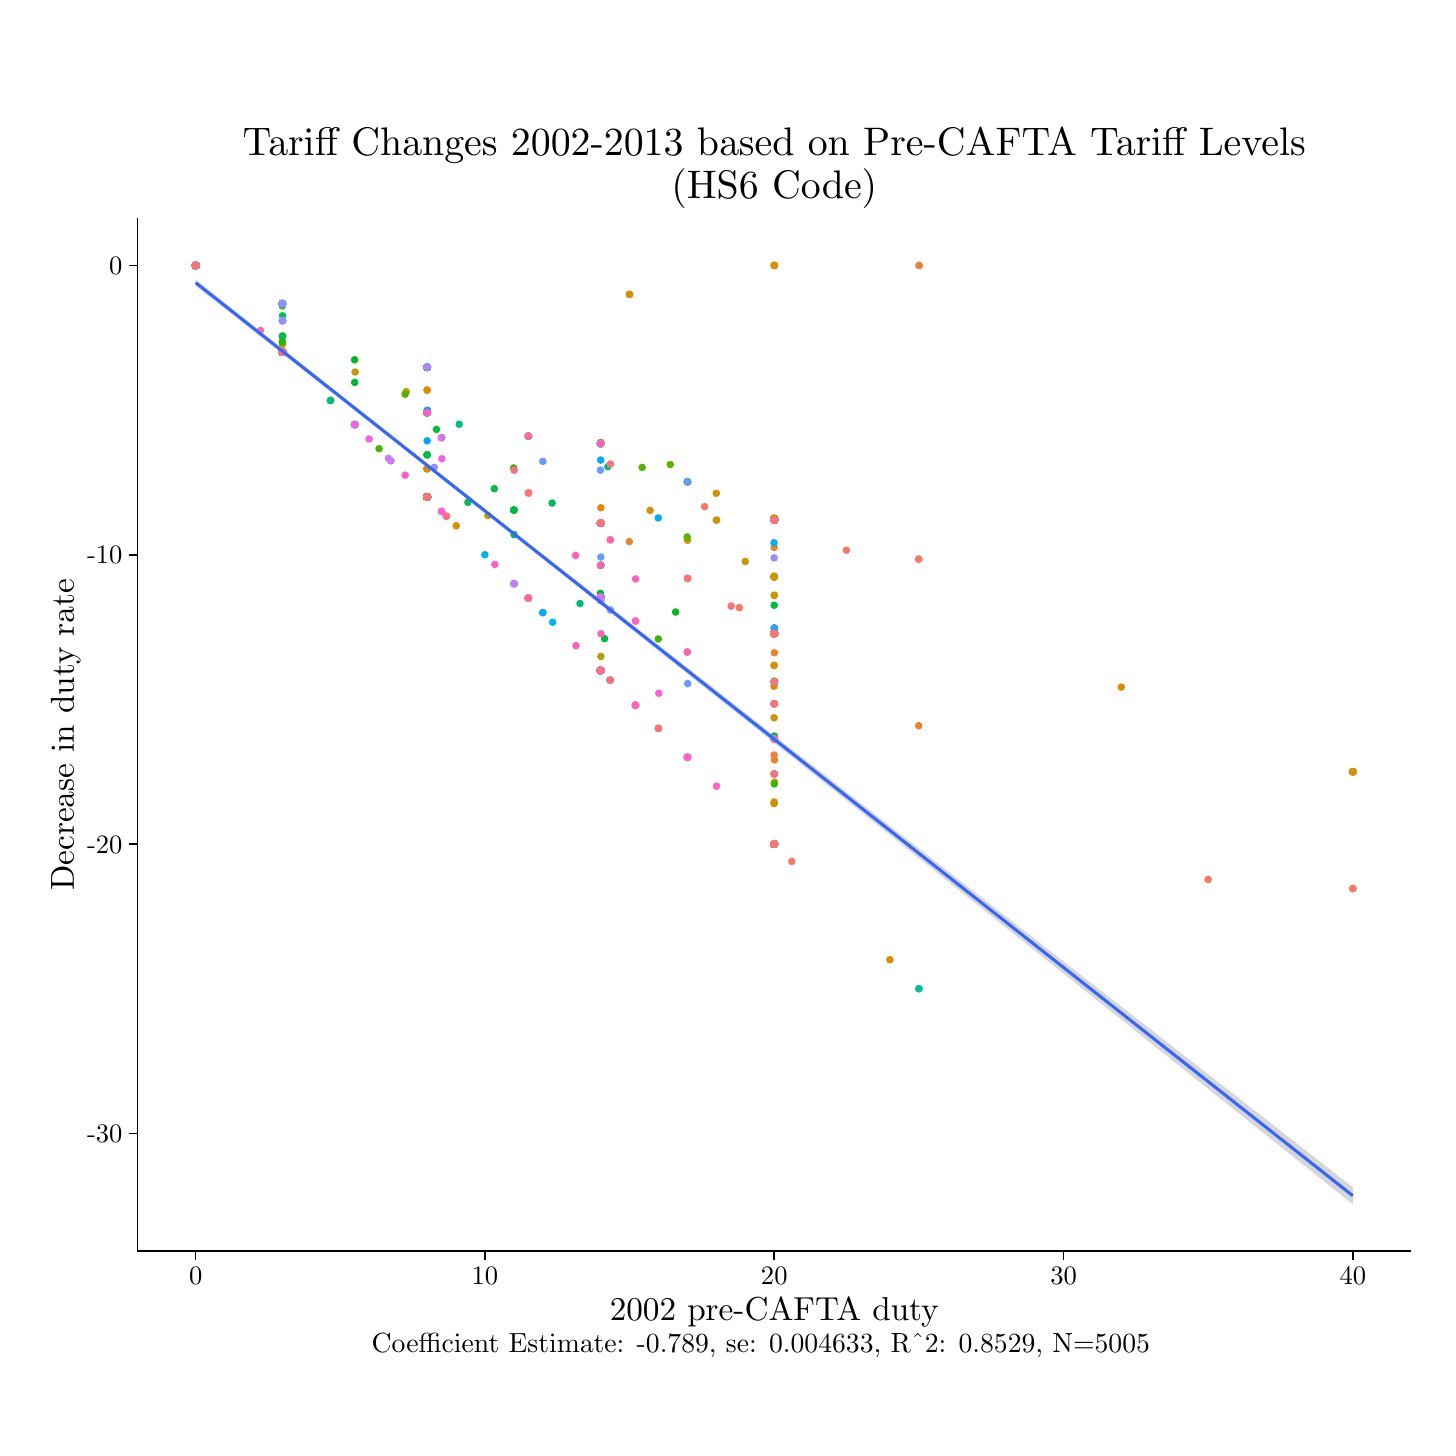
\begin{tikzpicture}[x=1pt,y=1pt]
\definecolor{fillColor}{RGB}{255,255,255}
\path[use as bounding box,fill=fillColor,fill opacity=0.00] (0,0) rectangle (505.89,505.89);
\begin{scope}
\path[clip] (  0.00, 30.28) rectangle (505.89,475.61);
\definecolor{drawColor}{RGB}{255,255,255}
\definecolor{fillColor}{RGB}{255,255,255}

\path[draw=drawColor,line width= 0.6pt,line join=round,line cap=round,fill=fillColor] (  0.00, 30.28) rectangle (505.89,475.61);
\end{scope}
\begin{scope}
\path[clip] ( 39.66, 63.75) rectangle (499.89,436.94);
\definecolor{fillColor}{RGB}{255,255,255}

\path[fill=fillColor] ( 39.66, 63.75) rectangle (499.89,436.94);
\definecolor{drawColor}{RGB}{248,118,109}
\definecolor{fillColor}{RGB}{248,118,109}

\path[draw=drawColor,line width= 0.4pt,line join=round,line cap=round,fill=fillColor] ( 60.77,419.96) circle (  1.16);

\path[draw=drawColor,line width= 0.4pt,line join=round,line cap=round,fill=fillColor] (144.21,336.33) circle (  1.16);

\path[draw=drawColor,line width= 0.4pt,line join=round,line cap=round,fill=fillColor] ( 60.63,419.96) circle (  1.16);
\definecolor{drawColor}{RGB}{248,118,108}
\definecolor{fillColor}{RGB}{248,118,108}

\path[draw=drawColor,line width= 0.4pt,line join=round,line cap=round,fill=fillColor] (144.38,336.33) circle (  1.16);

\path[draw=drawColor,line width= 0.4pt,line join=round,line cap=round,fill=fillColor] ( 60.59,419.96) circle (  1.16);

\path[draw=drawColor,line width= 0.4pt,line join=round,line cap=round,fill=fillColor] (144.22,336.35) circle (  1.16);
\definecolor{drawColor}{RGB}{248,119,108}
\definecolor{fillColor}{RGB}{248,119,108}

\path[draw=drawColor,line width= 0.4pt,line join=round,line cap=round,fill=fillColor] (144.31,336.33) circle (  1.16);

\path[draw=drawColor,line width= 0.4pt,line join=round,line cap=round,fill=fillColor] (144.33,336.33) circle (  1.16);
\definecolor{drawColor}{RGB}{248,119,107}
\definecolor{fillColor}{RGB}{248,119,107}

\path[draw=drawColor,line width= 0.4pt,line join=round,line cap=round,fill=fillColor] (144.33,336.34) circle (  1.16);
\definecolor{drawColor}{RGB}{247,119,107}
\definecolor{fillColor}{RGB}{247,119,107}

\path[draw=drawColor,line width= 0.4pt,line join=round,line cap=round,fill=fillColor] ( 60.73,419.97) circle (  1.16);

\path[draw=drawColor,line width= 0.4pt,line join=round,line cap=round,fill=fillColor] (144.39,336.32) circle (  1.16);

\path[draw=drawColor,line width= 0.4pt,line join=round,line cap=round,fill=fillColor] (144.33,336.34) circle (  1.16);

\path[draw=drawColor,line width= 0.4pt,line join=round,line cap=round,fill=fillColor] (144.36,336.32) circle (  1.16);
\definecolor{drawColor}{RGB}{247,119,106}
\definecolor{fillColor}{RGB}{247,119,106}

\path[draw=drawColor,line width= 0.4pt,line join=round,line cap=round,fill=fillColor] (144.30,336.33) circle (  1.16);

\path[draw=drawColor,line width= 0.4pt,line join=round,line cap=round,fill=fillColor] (144.31,336.34) circle (  1.16);

\path[draw=drawColor,line width= 0.4pt,line join=round,line cap=round,fill=fillColor] (144.43,336.35) circle (  1.16);

\path[draw=drawColor,line width= 0.4pt,line join=round,line cap=round,fill=fillColor] (478.86,237.02) circle (  1.16);

\path[draw=drawColor,line width= 0.4pt,line join=round,line cap=round,fill=fillColor] (478.94,237.03) circle (  1.16);

\path[draw=drawColor,line width= 0.4pt,line join=round,line cap=round,fill=fillColor] (478.88,237.01) circle (  1.16);
\definecolor{drawColor}{RGB}{247,119,105}
\definecolor{fillColor}{RGB}{247,119,105}

\path[draw=drawColor,line width= 0.4pt,line join=round,line cap=round,fill=fillColor] (478.89,237.01) circle (  1.16);

\path[draw=drawColor,line width= 0.4pt,line join=round,line cap=round,fill=fillColor] (478.96,237.01) circle (  1.16);

\path[draw=drawColor,line width= 0.4pt,line join=round,line cap=round,fill=fillColor] (295.86,317.05) circle (  1.16);
\definecolor{drawColor}{RGB}{247,120,104}
\definecolor{fillColor}{RGB}{247,120,104}

\path[draw=drawColor,line width= 0.4pt,line join=round,line cap=round,fill=fillColor] (269.74,286.92) circle (  1.16);
\definecolor{drawColor}{RGB}{247,120,103}
\definecolor{fillColor}{RGB}{247,120,103}

\path[draw=drawColor,line width= 0.4pt,line join=round,line cap=round,fill=fillColor] (269.68,286.92) circle (  1.16);

\path[draw=drawColor,line width= 0.4pt,line join=round,line cap=round,fill=fillColor] (269.89,286.93) circle (  1.16);
\definecolor{drawColor}{RGB}{246,120,103}
\definecolor{fillColor}{RGB}{246,120,103}

\path[draw=drawColor,line width= 0.4pt,line join=round,line cap=round,fill=fillColor] (269.83,286.91) circle (  1.16);

\path[draw=drawColor,line width= 0.4pt,line join=round,line cap=round,fill=fillColor] (269.67,286.93) circle (  1.16);

\path[draw=drawColor,line width= 0.4pt,line join=round,line cap=round,fill=fillColor] (269.78,286.91) circle (  1.16);
\definecolor{drawColor}{RGB}{246,120,102}
\definecolor{fillColor}{RGB}{246,120,102}

\path[draw=drawColor,line width= 0.4pt,line join=round,line cap=round,fill=fillColor] (269.88,286.92) circle (  1.16);

\path[draw=drawColor,line width= 0.4pt,line join=round,line cap=round,fill=fillColor] (269.75,286.91) circle (  1.16);

\path[draw=drawColor,line width= 0.4pt,line join=round,line cap=round,fill=fillColor] (269.81,286.91) circle (  1.16);

\path[draw=drawColor,line width= 0.4pt,line join=round,line cap=round,fill=fillColor] (269.78,286.92) circle (  1.16);

\path[draw=drawColor,line width= 0.4pt,line join=round,line cap=round,fill=fillColor] (478.97,237.01) circle (  1.16);
\definecolor{drawColor}{RGB}{246,120,101}
\definecolor{fillColor}{RGB}{246,120,101}

\path[draw=drawColor,line width= 0.4pt,line join=round,line cap=round,fill=fillColor] (478.85,237.02) circle (  1.16);

\path[draw=drawColor,line width= 0.4pt,line join=round,line cap=round,fill=fillColor] (478.89,237.02) circle (  1.16);

\path[draw=drawColor,line width= 0.4pt,line join=round,line cap=round,fill=fillColor] (478.78,237.02) circle (  1.16);

\path[draw=drawColor,line width= 0.4pt,line join=round,line cap=round,fill=fillColor] (478.75,237.02) circle (  1.16);

\path[draw=drawColor,line width= 0.4pt,line join=round,line cap=round,fill=fillColor] (478.92,237.02) circle (  1.16);
\definecolor{drawColor}{RGB}{246,120,100}
\definecolor{fillColor}{RGB}{246,120,100}

\path[draw=drawColor,line width= 0.4pt,line join=round,line cap=round,fill=fillColor] (478.83,237.01) circle (  1.16);
\definecolor{drawColor}{RGB}{246,121,100}
\definecolor{fillColor}{RGB}{246,121,100}

\path[draw=drawColor,line width= 0.4pt,line join=round,line cap=round,fill=fillColor] (269.86,328.49) circle (  1.16);

\path[draw=drawColor,line width= 0.4pt,line join=round,line cap=round,fill=fillColor] (269.88,328.49) circle (  1.16);

\path[draw=drawColor,line width= 0.4pt,line join=round,line cap=round,fill=fillColor] (321.93,313.86) circle (  1.16);

\path[draw=drawColor,line width= 0.4pt,line join=round,line cap=round,fill=fillColor] (322.01,313.85) circle (  1.16);
\definecolor{drawColor}{RGB}{246,121,99}
\definecolor{fillColor}{RGB}{246,121,99}

\path[draw=drawColor,line width= 0.4pt,line join=round,line cap=round,fill=fillColor] (276.12,204.62) circle (  1.16);

\path[draw=drawColor,line width= 0.4pt,line join=round,line cap=round,fill=fillColor] (269.79,210.88) circle (  1.16);
\definecolor{drawColor}{RGB}{245,121,99}
\definecolor{fillColor}{RGB}{245,121,99}

\path[draw=drawColor,line width= 0.4pt,line join=round,line cap=round,fill=fillColor] (269.74,210.90) circle (  1.16);

\path[draw=drawColor,line width= 0.4pt,line join=round,line cap=round,fill=fillColor] (257.14,296.32) circle (  1.16);
\definecolor{drawColor}{RGB}{245,121,98}
\definecolor{fillColor}{RGB}{245,121,98}

\path[draw=drawColor,line width= 0.4pt,line join=round,line cap=round,fill=fillColor] (244.62,332.80) circle (  1.16);

\path[draw=drawColor,line width= 0.4pt,line join=round,line cap=round,fill=fillColor] (269.85,328.49) circle (  1.16);

\path[draw=drawColor,line width= 0.4pt,line join=round,line cap=round,fill=fillColor] (269.67,328.50) circle (  1.16);

\path[draw=drawColor,line width= 0.4pt,line join=round,line cap=round,fill=fillColor] (206.99,326.84) circle (  1.16);

\path[draw=drawColor,line width= 0.4pt,line join=round,line cap=round,fill=fillColor] (269.77,286.91) circle (  1.16);
\definecolor{drawColor}{RGB}{245,121,97}
\definecolor{fillColor}{RGB}{245,121,97}

\path[draw=drawColor,line width= 0.4pt,line join=round,line cap=round,fill=fillColor] (269.71,286.90) circle (  1.16);

\path[draw=drawColor,line width= 0.4pt,line join=round,line cap=round,fill=fillColor] (269.86,210.90) circle (  1.16);

\path[draw=drawColor,line width= 0.4pt,line join=round,line cap=round,fill=fillColor] (269.70,210.89) circle (  1.16);

\path[draw=drawColor,line width= 0.4pt,line join=round,line cap=round,fill=fillColor] (269.84,210.89) circle (  1.16);

\path[draw=drawColor,line width= 0.4pt,line join=round,line cap=round,fill=fillColor] (426.56,198.08) circle (  1.16);
\definecolor{drawColor}{RGB}{245,122,96}
\definecolor{fillColor}{RGB}{245,122,96}

\path[draw=drawColor,line width= 0.4pt,line join=round,line cap=round,fill=fillColor] (478.85,194.81) circle (  1.16);

\path[draw=drawColor,line width= 0.4pt,line join=round,line cap=round,fill=fillColor] (478.88,194.81) circle (  1.16);

\path[draw=drawColor,line width= 0.4pt,line join=round,line cap=round,fill=fillColor] (478.82,194.80) circle (  1.16);

\path[draw=drawColor,line width= 0.4pt,line join=round,line cap=round,fill=fillColor] (207.07,273.60) circle (  1.16);
\definecolor{drawColor}{RGB}{245,122,95}
\definecolor{fillColor}{RGB}{245,122,95}

\path[draw=drawColor,line width= 0.4pt,line join=round,line cap=round,fill=fillColor] (269.87,210.90) circle (  1.16);

\path[draw=drawColor,line width= 0.4pt,line join=round,line cap=round,fill=fillColor] (269.67,210.90) circle (  1.16);

\path[draw=drawColor,line width= 0.4pt,line join=round,line cap=round,fill=fillColor] (269.71,210.87) circle (  1.16);
\definecolor{drawColor}{RGB}{244,122,95}
\definecolor{fillColor}{RGB}{244,122,95}

\path[draw=drawColor,line width= 0.4pt,line join=round,line cap=round,fill=fillColor] (269.81,210.89) circle (  1.16);

\path[draw=drawColor,line width= 0.4pt,line join=round,line cap=round,fill=fillColor] (269.85,210.88) circle (  1.16);
\definecolor{drawColor}{RGB}{244,122,94}
\definecolor{fillColor}{RGB}{244,122,94}

\path[draw=drawColor,line width= 0.4pt,line join=round,line cap=round,fill=fillColor] (269.89,210.88) circle (  1.16);

\path[draw=drawColor,line width= 0.4pt,line join=round,line cap=round,fill=fillColor] (269.87,210.89) circle (  1.16);

\path[draw=drawColor,line width= 0.4pt,line join=round,line cap=round,fill=fillColor] (269.78,210.90) circle (  1.16);

\path[draw=drawColor,line width= 0.4pt,line join=round,line cap=round,fill=fillColor] (269.81,210.90) circle (  1.16);

\path[draw=drawColor,line width= 0.4pt,line join=round,line cap=round,fill=fillColor] (269.81,210.90) circle (  1.16);
\definecolor{drawColor}{RGB}{244,122,93}
\definecolor{fillColor}{RGB}{244,122,93}

\path[draw=drawColor,line width= 0.4pt,line join=round,line cap=round,fill=fillColor] (269.78,210.88) circle (  1.16);

\path[draw=drawColor,line width= 0.4pt,line join=round,line cap=round,fill=fillColor] (269.84,210.89) circle (  1.16);

\path[draw=drawColor,line width= 0.4pt,line join=round,line cap=round,fill=fillColor] (269.79,210.89) circle (  1.16);

\path[draw=drawColor,line width= 0.4pt,line join=round,line cap=round,fill=fillColor] (269.69,210.89) circle (  1.16);

\path[draw=drawColor,line width= 0.4pt,line join=round,line cap=round,fill=fillColor] (269.82,210.90) circle (  1.16);
\definecolor{drawColor}{RGB}{244,123,92}
\definecolor{fillColor}{RGB}{244,123,92}

\path[draw=drawColor,line width= 0.4pt,line join=round,line cap=round,fill=fillColor] (269.80,210.89) circle (  1.16);

\path[draw=drawColor,line width= 0.4pt,line join=round,line cap=round,fill=fillColor] (269.79,210.89) circle (  1.16);

\path[draw=drawColor,line width= 0.4pt,line join=round,line cap=round,fill=fillColor] (269.88,210.89) circle (  1.16);

\path[draw=drawColor,line width= 0.4pt,line join=round,line cap=round,fill=fillColor] (269.74,210.89) circle (  1.16);
\definecolor{drawColor}{RGB}{244,123,91}
\definecolor{fillColor}{RGB}{244,123,91}

\path[draw=drawColor,line width= 0.4pt,line join=round,line cap=round,fill=fillColor] (269.77,210.89) circle (  1.16);

\path[draw=drawColor,line width= 0.4pt,line join=round,line cap=round,fill=fillColor] (269.84,210.90) circle (  1.16);

\path[draw=drawColor,line width= 0.4pt,line join=round,line cap=round,fill=fillColor] (269.80,210.89) circle (  1.16);

\path[draw=drawColor,line width= 0.4pt,line join=round,line cap=round,fill=fillColor] (269.72,210.87) circle (  1.16);
\definecolor{drawColor}{RGB}{243,123,91}
\definecolor{fillColor}{RGB}{243,123,91}

\path[draw=drawColor,line width= 0.4pt,line join=round,line cap=round,fill=fillColor] (269.89,210.88) circle (  1.16);
\definecolor{drawColor}{RGB}{243,123,90}
\definecolor{fillColor}{RGB}{243,123,90}

\path[draw=drawColor,line width= 0.4pt,line join=round,line cap=round,fill=fillColor] (269.84,210.90) circle (  1.16);

\path[draw=drawColor,line width= 0.4pt,line join=round,line cap=round,fill=fillColor] (269.76,210.88) circle (  1.16);

\path[draw=drawColor,line width= 0.4pt,line join=round,line cap=round,fill=fillColor] (269.76,210.88) circle (  1.16);

\path[draw=drawColor,line width= 0.4pt,line join=round,line cap=round,fill=fillColor] (269.87,210.90) circle (  1.16);

\path[draw=drawColor,line width= 0.4pt,line join=round,line cap=round,fill=fillColor] (269.88,210.89) circle (  1.16);
\definecolor{drawColor}{RGB}{243,123,89}
\definecolor{fillColor}{RGB}{243,123,89}

\path[draw=drawColor,line width= 0.4pt,line join=round,line cap=round,fill=fillColor] (269.73,210.88) circle (  1.16);

\path[draw=drawColor,line width= 0.4pt,line join=round,line cap=round,fill=fillColor] (269.75,210.88) circle (  1.16);

\path[draw=drawColor,line width= 0.4pt,line join=round,line cap=round,fill=fillColor] (269.87,210.89) circle (  1.16);

\path[draw=drawColor,line width= 0.4pt,line join=round,line cap=round,fill=fillColor] (269.74,210.90) circle (  1.16);
\definecolor{drawColor}{RGB}{243,123,88}
\definecolor{fillColor}{RGB}{243,123,88}

\path[draw=drawColor,line width= 0.4pt,line join=round,line cap=round,fill=fillColor] (269.83,210.90) circle (  1.16);
\definecolor{drawColor}{RGB}{243,124,88}
\definecolor{fillColor}{RGB}{243,124,88}

\path[draw=drawColor,line width= 0.4pt,line join=round,line cap=round,fill=fillColor] ( 92.01,388.61) circle (  1.16);

\path[draw=drawColor,line width= 0.4pt,line join=round,line cap=round,fill=fillColor] ( 92.15,388.60) circle (  1.16);

\path[draw=drawColor,line width= 0.4pt,line join=round,line cap=round,fill=fillColor] ( 92.02,388.59) circle (  1.16);

\path[draw=drawColor,line width= 0.4pt,line join=round,line cap=round,fill=fillColor] ( 92.13,388.62) circle (  1.16);
\definecolor{drawColor}{RGB}{243,124,87}
\definecolor{fillColor}{RGB}{243,124,87}

\path[draw=drawColor,line width= 0.4pt,line join=round,line cap=round,fill=fillColor] ( 92.07,388.60) circle (  1.16);

\path[draw=drawColor,line width= 0.4pt,line join=round,line cap=round,fill=fillColor] ( 92.00,388.61) circle (  1.16);

\path[draw=drawColor,line width= 0.4pt,line join=round,line cap=round,fill=fillColor] ( 92.04,388.60) circle (  1.16);

\path[draw=drawColor,line width= 0.4pt,line join=round,line cap=round,fill=fillColor] (269.68,210.89) circle (  1.16);
\definecolor{drawColor}{RGB}{242,124,87}
\definecolor{fillColor}{RGB}{242,124,87}

\path[draw=drawColor,line width= 0.4pt,line join=round,line cap=round,fill=fillColor] (269.75,210.90) circle (  1.16);
\definecolor{drawColor}{RGB}{242,124,86}
\definecolor{fillColor}{RGB}{242,124,86}

\path[draw=drawColor,line width= 0.4pt,line join=round,line cap=round,fill=fillColor] (269.66,210.89) circle (  1.16);

\path[draw=drawColor,line width= 0.4pt,line join=round,line cap=round,fill=fillColor] (269.80,210.89) circle (  1.16);

\path[draw=drawColor,line width= 0.4pt,line join=round,line cap=round,fill=fillColor] (269.85,210.90) circle (  1.16);

\path[draw=drawColor,line width= 0.4pt,line join=round,line cap=round,fill=fillColor] (269.83,210.90) circle (  1.16);
\definecolor{drawColor}{RGB}{242,124,85}
\definecolor{fillColor}{RGB}{242,124,85}

\path[draw=drawColor,line width= 0.4pt,line join=round,line cap=round,fill=fillColor] ( 92.16,388.61) circle (  1.16);

\path[draw=drawColor,line width= 0.4pt,line join=round,line cap=round,fill=fillColor] (269.73,210.90) circle (  1.16);

\path[draw=drawColor,line width= 0.4pt,line join=round,line cap=round,fill=fillColor] (269.77,210.88) circle (  1.16);

\path[draw=drawColor,line width= 0.4pt,line join=round,line cap=round,fill=fillColor] (269.87,210.89) circle (  1.16);

\path[draw=drawColor,line width= 0.4pt,line join=round,line cap=round,fill=fillColor] (269.84,210.88) circle (  1.16);
\definecolor{drawColor}{RGB}{242,124,84}
\definecolor{fillColor}{RGB}{242,124,84}

\path[draw=drawColor,line width= 0.4pt,line join=round,line cap=round,fill=fillColor] (269.85,210.88) circle (  1.16);

\path[draw=drawColor,line width= 0.4pt,line join=round,line cap=round,fill=fillColor] (206.96,273.61) circle (  1.16);
\definecolor{drawColor}{RGB}{242,125,84}
\definecolor{fillColor}{RGB}{242,125,84}

\path[draw=drawColor,line width= 0.4pt,line join=round,line cap=round,fill=fillColor] (207.08,273.61) circle (  1.16);

\path[draw=drawColor,line width= 0.4pt,line join=round,line cap=round,fill=fillColor] (269.88,210.88) circle (  1.16);
\definecolor{drawColor}{RGB}{242,125,83}
\definecolor{fillColor}{RGB}{242,125,83}

\path[draw=drawColor,line width= 0.4pt,line join=round,line cap=round,fill=fillColor] (269.84,210.88) circle (  1.16);

\path[draw=drawColor,line width= 0.4pt,line join=round,line cap=round,fill=fillColor] ( 60.61,419.98) circle (  1.16);

\path[draw=drawColor,line width= 0.4pt,line join=round,line cap=round,fill=fillColor] (269.71,210.90) circle (  1.16);

\path[draw=drawColor,line width= 0.4pt,line join=round,line cap=round,fill=fillColor] (144.39,336.33) circle (  1.16);

\path[draw=drawColor,line width= 0.4pt,line join=round,line cap=round,fill=fillColor] (206.95,273.60) circle (  1.16);
\definecolor{drawColor}{RGB}{241,125,82}
\definecolor{fillColor}{RGB}{241,125,82}

\path[draw=drawColor,line width= 0.4pt,line join=round,line cap=round,fill=fillColor] (144.40,336.33) circle (  1.16);

\path[draw=drawColor,line width= 0.4pt,line join=round,line cap=round,fill=fillColor] ( 60.58,419.97) circle (  1.16);

\path[draw=drawColor,line width= 0.4pt,line join=round,line cap=round,fill=fillColor] (269.71,210.89) circle (  1.16);

\path[draw=drawColor,line width= 0.4pt,line join=round,line cap=round,fill=fillColor] (269.66,210.88) circle (  1.16);
\definecolor{drawColor}{RGB}{241,125,81}
\definecolor{fillColor}{RGB}{241,125,81}

\path[draw=drawColor,line width= 0.4pt,line join=round,line cap=round,fill=fillColor] (269.76,210.90) circle (  1.16);

\path[draw=drawColor,line width= 0.4pt,line join=round,line cap=round,fill=fillColor] (269.71,210.89) circle (  1.16);

\path[draw=drawColor,line width= 0.4pt,line join=round,line cap=round,fill=fillColor] (269.84,327.97) circle (  1.16);

\path[draw=drawColor,line width= 0.4pt,line join=round,line cap=round,fill=fillColor] (269.74,286.92) circle (  1.16);
\definecolor{drawColor}{RGB}{241,125,80}
\definecolor{fillColor}{RGB}{241,125,80}

\path[draw=drawColor,line width= 0.4pt,line join=round,line cap=round,fill=fillColor] (269.78,307.44) circle (  1.16);

\path[draw=drawColor,line width= 0.4pt,line join=round,line cap=round,fill=fillColor] (269.84,210.88) circle (  1.16);

\path[draw=drawColor,line width= 0.4pt,line join=round,line cap=round,fill=fillColor] (269.67,210.90) circle (  1.16);

\path[draw=drawColor,line width= 0.4pt,line join=round,line cap=round,fill=fillColor] (269.71,210.89) circle (  1.16);
\definecolor{drawColor}{RGB}{241,126,80}
\definecolor{fillColor}{RGB}{241,126,80}

\path[draw=drawColor,line width= 0.4pt,line join=round,line cap=round,fill=fillColor] (269.83,210.89) circle (  1.16);
\definecolor{drawColor}{RGB}{241,126,79}
\definecolor{fillColor}{RGB}{241,126,79}

\path[draw=drawColor,line width= 0.4pt,line join=round,line cap=round,fill=fillColor] (227.90,252.71) circle (  1.16);

\path[draw=drawColor,line width= 0.4pt,line join=round,line cap=round,fill=fillColor] (269.85,210.88) circle (  1.16);

\path[draw=drawColor,line width= 0.4pt,line join=round,line cap=round,fill=fillColor] (269.80,210.89) circle (  1.16);

\path[draw=drawColor,line width= 0.4pt,line join=round,line cap=round,fill=fillColor] (269.76,210.90) circle (  1.16);
\definecolor{drawColor}{RGB}{241,126,78}
\definecolor{fillColor}{RGB}{241,126,78}

\path[draw=drawColor,line width= 0.4pt,line join=round,line cap=round,fill=fillColor] (269.86,210.89) circle (  1.16);
\definecolor{drawColor}{RGB}{240,126,78}
\definecolor{fillColor}{RGB}{240,126,78}

\path[draw=drawColor,line width= 0.4pt,line join=round,line cap=round,fill=fillColor] (269.85,286.93) circle (  1.16);

\path[draw=drawColor,line width= 0.4pt,line join=round,line cap=round,fill=fillColor] (269.68,210.89) circle (  1.16);

\path[draw=drawColor,line width= 0.4pt,line join=round,line cap=round,fill=fillColor] (269.78,210.90) circle (  1.16);
\definecolor{drawColor}{RGB}{240,126,77}
\definecolor{fillColor}{RGB}{240,126,77}

\path[draw=drawColor,line width= 0.4pt,line join=round,line cap=round,fill=fillColor] (269.81,210.90) circle (  1.16);

\path[draw=drawColor,line width= 0.4pt,line join=round,line cap=round,fill=fillColor] (269.69,210.89) circle (  1.16);

\path[draw=drawColor,line width= 0.4pt,line join=round,line cap=round,fill=fillColor] (269.78,210.88) circle (  1.16);

\path[draw=drawColor,line width= 0.4pt,line join=round,line cap=round,fill=fillColor] (269.74,210.90) circle (  1.16);
\definecolor{drawColor}{RGB}{240,126,76}
\definecolor{fillColor}{RGB}{240,126,76}

\path[draw=drawColor,line width= 0.4pt,line join=round,line cap=round,fill=fillColor] (144.25,336.34) circle (  1.16);
\definecolor{drawColor}{RGB}{240,127,75}
\definecolor{fillColor}{RGB}{240,127,75}

\path[draw=drawColor,line width= 0.4pt,line join=round,line cap=round,fill=fillColor] (269.86,328.49) circle (  1.16);
\definecolor{drawColor}{RGB}{240,127,74}
\definecolor{fillColor}{RGB}{240,127,74}

\path[draw=drawColor,line width= 0.4pt,line join=round,line cap=round,fill=fillColor] (269.68,286.92) circle (  1.16);

\path[draw=drawColor,line width= 0.4pt,line join=round,line cap=round,fill=fillColor] (269.77,210.87) circle (  1.16);
\definecolor{drawColor}{RGB}{239,127,74}
\definecolor{fillColor}{RGB}{239,127,74}

\path[draw=drawColor,line width= 0.4pt,line join=round,line cap=round,fill=fillColor] ( 92.10,388.61) circle (  1.16);

\path[draw=drawColor,line width= 0.4pt,line join=round,line cap=round,fill=fillColor] (207.12,273.60) circle (  1.16);
\definecolor{drawColor}{RGB}{239,127,73}
\definecolor{fillColor}{RGB}{239,127,73}

\path[draw=drawColor,line width= 0.4pt,line join=round,line cap=round,fill=fillColor] (269.81,286.93) circle (  1.16);

\path[draw=drawColor,line width= 0.4pt,line join=round,line cap=round,fill=fillColor] (238.53,242.25) circle (  1.16);
\definecolor{drawColor}{RGB}{239,127,71}
\definecolor{fillColor}{RGB}{239,127,71}

\path[draw=drawColor,line width= 0.4pt,line join=round,line cap=round,fill=fillColor] (269.74,269.69) circle (  1.16);

\path[draw=drawColor,line width= 0.4pt,line join=round,line cap=round,fill=fillColor] (144.40,336.34) circle (  1.16);

\path[draw=drawColor,line width= 0.4pt,line join=round,line cap=round,fill=fillColor] (144.27,366.74) circle (  1.16);
\definecolor{drawColor}{RGB}{239,127,70}
\definecolor{fillColor}{RGB}{239,127,70}

\path[draw=drawColor,line width= 0.4pt,line join=round,line cap=round,fill=fillColor] (144.32,336.33) circle (  1.16);

\path[draw=drawColor,line width= 0.4pt,line join=round,line cap=round,fill=fillColor] (144.24,366.75) circle (  1.16);
\definecolor{drawColor}{RGB}{239,128,70}
\definecolor{fillColor}{RGB}{239,128,70}

\path[draw=drawColor,line width= 0.4pt,line join=round,line cap=round,fill=fillColor] (269.87,286.90) circle (  1.16);

\path[draw=drawColor,line width= 0.4pt,line join=round,line cap=round,fill=fillColor] (269.75,210.89) circle (  1.16);
\definecolor{drawColor}{RGB}{238,128,69}
\definecolor{fillColor}{RGB}{238,128,69}

\path[draw=drawColor,line width= 0.4pt,line join=round,line cap=round,fill=fillColor] ( 60.81,419.97) circle (  1.16);

\path[draw=drawColor,line width= 0.4pt,line join=round,line cap=round,fill=fillColor] ( 60.65,419.96) circle (  1.16);

\path[draw=drawColor,line width= 0.4pt,line join=round,line cap=round,fill=fillColor] ( 60.77,419.97) circle (  1.16);

\path[draw=drawColor,line width= 0.4pt,line join=round,line cap=round,fill=fillColor] ( 60.61,419.96) circle (  1.16);
\definecolor{drawColor}{RGB}{238,128,68}
\definecolor{fillColor}{RGB}{238,128,68}

\path[draw=drawColor,line width= 0.4pt,line join=round,line cap=round,fill=fillColor] (144.26,366.74) circle (  1.16);

\path[draw=drawColor,line width= 0.4pt,line join=round,line cap=round,fill=fillColor] ( 60.72,419.96) circle (  1.16);

\path[draw=drawColor,line width= 0.4pt,line join=round,line cap=round,fill=fillColor] ( 92.12,388.61) circle (  1.16);

\path[draw=drawColor,line width= 0.4pt,line join=round,line cap=round,fill=fillColor] ( 60.67,419.98) circle (  1.16);
\definecolor{drawColor}{RGB}{238,128,67}
\definecolor{fillColor}{RGB}{238,128,67}

\path[draw=drawColor,line width= 0.4pt,line join=round,line cap=round,fill=fillColor] ( 60.69,419.97) circle (  1.16);

\path[draw=drawColor,line width= 0.4pt,line join=round,line cap=round,fill=fillColor] ( 60.75,419.97) circle (  1.16);

\path[draw=drawColor,line width= 0.4pt,line join=round,line cap=round,fill=fillColor] ( 60.72,419.96) circle (  1.16);

\path[draw=drawColor,line width= 0.4pt,line join=round,line cap=round,fill=fillColor] ( 60.73,419.95) circle (  1.16);
\definecolor{drawColor}{RGB}{238,128,66}
\definecolor{fillColor}{RGB}{238,128,66}

\path[draw=drawColor,line width= 0.4pt,line join=round,line cap=round,fill=fillColor] ( 60.78,419.96) circle (  1.16);

\path[draw=drawColor,line width= 0.4pt,line join=round,line cap=round,fill=fillColor] ( 60.64,419.96) circle (  1.16);

\path[draw=drawColor,line width= 0.4pt,line join=round,line cap=round,fill=fillColor] ( 60.77,419.96) circle (  1.16);
\definecolor{drawColor}{RGB}{238,128,65}
\definecolor{fillColor}{RGB}{238,128,65}

\path[draw=drawColor,line width= 0.4pt,line join=round,line cap=round,fill=fillColor] ( 60.65,419.96) circle (  1.16);

\path[draw=drawColor,line width= 0.4pt,line join=round,line cap=round,fill=fillColor] ( 60.61,419.98) circle (  1.16);
\definecolor{drawColor}{RGB}{237,129,65}
\definecolor{fillColor}{RGB}{237,129,65}

\path[draw=drawColor,line width= 0.4pt,line join=round,line cap=round,fill=fillColor] ( 60.66,419.98) circle (  1.16);

\path[draw=drawColor,line width= 0.4pt,line join=round,line cap=round,fill=fillColor] ( 60.71,419.98) circle (  1.16);
\definecolor{drawColor}{RGB}{237,129,64}
\definecolor{fillColor}{RGB}{237,129,64}

\path[draw=drawColor,line width= 0.4pt,line join=round,line cap=round,fill=fillColor] ( 60.72,419.98) circle (  1.16);

\path[draw=drawColor,line width= 0.4pt,line join=round,line cap=round,fill=fillColor] ( 60.69,419.96) circle (  1.16);

\path[draw=drawColor,line width= 0.4pt,line join=round,line cap=round,fill=fillColor] ( 60.80,419.96) circle (  1.16);

\path[draw=drawColor,line width= 0.4pt,line join=round,line cap=round,fill=fillColor] ( 60.76,419.96) circle (  1.16);
\definecolor{drawColor}{RGB}{237,129,63}
\definecolor{fillColor}{RGB}{237,129,63}

\path[draw=drawColor,line width= 0.4pt,line join=round,line cap=round,fill=fillColor] ( 60.63,419.97) circle (  1.16);

\path[draw=drawColor,line width= 0.4pt,line join=round,line cap=round,fill=fillColor] (269.85,328.49) circle (  1.16);

\path[draw=drawColor,line width= 0.4pt,line join=round,line cap=round,fill=fillColor] (269.74,210.89) circle (  1.16);
\definecolor{drawColor}{RGB}{237,129,62}
\definecolor{fillColor}{RGB}{237,129,62}

\path[draw=drawColor,line width= 0.4pt,line join=round,line cap=round,fill=fillColor] (269.81,210.90) circle (  1.16);

\path[draw=drawColor,line width= 0.4pt,line join=round,line cap=round,fill=fillColor] (269.68,210.89) circle (  1.16);

\path[draw=drawColor,line width= 0.4pt,line join=round,line cap=round,fill=fillColor] (269.71,210.90) circle (  1.16);

\path[draw=drawColor,line width= 0.4pt,line join=round,line cap=round,fill=fillColor] ( 60.63,419.98) circle (  1.16);
\definecolor{drawColor}{RGB}{237,129,61}
\definecolor{fillColor}{RGB}{237,129,61}

\path[draw=drawColor,line width= 0.4pt,line join=round,line cap=round,fill=fillColor] (269.69,307.40) circle (  1.16);

\path[draw=drawColor,line width= 0.4pt,line join=round,line cap=round,fill=fillColor] (269.74,210.89) circle (  1.16);

\path[draw=drawColor,line width= 0.4pt,line join=round,line cap=round,fill=fillColor] (322.13,419.96) circle (  1.16);
\definecolor{drawColor}{RGB}{236,129,60}
\definecolor{fillColor}{RGB}{236,129,60}

\path[draw=drawColor,line width= 0.4pt,line join=round,line cap=round,fill=fillColor] (322.11,419.97) circle (  1.16);

\path[draw=drawColor,line width= 0.4pt,line join=round,line cap=round,fill=fillColor] (269.83,210.89) circle (  1.16);

\path[draw=drawColor,line width= 0.4pt,line join=round,line cap=round,fill=fillColor] (269.68,210.88) circle (  1.16);
\definecolor{drawColor}{RGB}{236,130,60}
\definecolor{fillColor}{RGB}{236,130,60}

\path[draw=drawColor,line width= 0.4pt,line join=round,line cap=round,fill=fillColor] (269.72,210.88) circle (  1.16);
\definecolor{drawColor}{RGB}{236,130,59}
\definecolor{fillColor}{RGB}{236,130,59}

\path[draw=drawColor,line width= 0.4pt,line join=round,line cap=round,fill=fillColor] (269.69,210.90) circle (  1.16);

\path[draw=drawColor,line width= 0.4pt,line join=round,line cap=round,fill=fillColor] (269.72,328.49) circle (  1.16);

\path[draw=drawColor,line width= 0.4pt,line join=round,line cap=round,fill=fillColor] (269.79,210.90) circle (  1.16);
\definecolor{drawColor}{RGB}{236,130,58}
\definecolor{fillColor}{RGB}{236,130,58}

\path[draw=drawColor,line width= 0.4pt,line join=round,line cap=round,fill=fillColor] (269.69,210.89) circle (  1.16);

\path[draw=drawColor,line width= 0.4pt,line join=round,line cap=round,fill=fillColor] (269.84,210.88) circle (  1.16);

\path[draw=drawColor,line width= 0.4pt,line join=round,line cap=round,fill=fillColor] (269.72,243.06) circle (  1.16);
\definecolor{drawColor}{RGB}{236,130,57}
\definecolor{fillColor}{RGB}{236,130,57}

\path[draw=drawColor,line width= 0.4pt,line join=round,line cap=round,fill=fillColor] (269.83,210.89) circle (  1.16);

\path[draw=drawColor,line width= 0.4pt,line join=round,line cap=round,fill=fillColor] (269.87,210.88) circle (  1.16);

\path[draw=drawColor,line width= 0.4pt,line join=round,line cap=round,fill=fillColor] (269.76,210.90) circle (  1.16);

\path[draw=drawColor,line width= 0.4pt,line join=round,line cap=round,fill=fillColor] (269.70,210.89) circle (  1.16);
\definecolor{drawColor}{RGB}{236,130,56}
\definecolor{fillColor}{RGB}{236,130,56}

\path[draw=drawColor,line width= 0.4pt,line join=round,line cap=round,fill=fillColor] (269.89,269.69) circle (  1.16);

\path[draw=drawColor,line width= 0.4pt,line join=round,line cap=round,fill=fillColor] (269.85,210.90) circle (  1.16);

\path[draw=drawColor,line width= 0.4pt,line join=round,line cap=round,fill=fillColor] (269.72,210.90) circle (  1.16);
\definecolor{drawColor}{RGB}{235,130,55}
\definecolor{fillColor}{RGB}{235,130,55}

\path[draw=drawColor,line width= 0.4pt,line join=round,line cap=round,fill=fillColor] (269.75,210.89) circle (  1.16);

\path[draw=drawColor,line width= 0.4pt,line join=round,line cap=round,fill=fillColor] (269.83,210.89) circle (  1.16);

\path[draw=drawColor,line width= 0.4pt,line join=round,line cap=round,fill=fillColor] (269.66,210.89) circle (  1.16);
\definecolor{drawColor}{RGB}{235,130,54}
\definecolor{fillColor}{RGB}{235,130,54}

\path[draw=drawColor,line width= 0.4pt,line join=round,line cap=round,fill=fillColor] (269.77,210.89) circle (  1.16);

\path[draw=drawColor,line width= 0.4pt,line join=round,line cap=round,fill=fillColor] (269.86,286.92) circle (  1.16);

\path[draw=drawColor,line width= 0.4pt,line join=round,line cap=round,fill=fillColor] (269.70,210.87) circle (  1.16);
\definecolor{drawColor}{RGB}{235,131,53}
\definecolor{fillColor}{RGB}{235,131,53}

\path[draw=drawColor,line width= 0.4pt,line join=round,line cap=round,fill=fillColor] (269.72,225.58) circle (  1.16);

\path[draw=drawColor,line width= 0.4pt,line join=round,line cap=round,fill=fillColor] (269.66,286.92) circle (  1.16);

\path[draw=drawColor,line width= 0.4pt,line join=round,line cap=round,fill=fillColor] (269.81,210.90) circle (  1.16);
\definecolor{drawColor}{RGB}{235,131,52}
\definecolor{fillColor}{RGB}{235,131,52}

\path[draw=drawColor,line width= 0.4pt,line join=round,line cap=round,fill=fillColor] (269.84,210.90) circle (  1.16);

\path[draw=drawColor,line width= 0.4pt,line join=round,line cap=round,fill=fillColor] (269.82,286.93) circle (  1.16);

\path[draw=drawColor,line width= 0.4pt,line join=round,line cap=round,fill=fillColor] (269.83,210.88) circle (  1.16);
\definecolor{drawColor}{RGB}{235,131,51}
\definecolor{fillColor}{RGB}{235,131,51}

\path[draw=drawColor,line width= 0.4pt,line join=round,line cap=round,fill=fillColor] (269.69,328.49) circle (  1.16);

\path[draw=drawColor,line width= 0.4pt,line join=round,line cap=round,fill=fillColor] (269.72,286.92) circle (  1.16);

\path[draw=drawColor,line width= 0.4pt,line join=round,line cap=round,fill=fillColor] (269.76,286.92) circle (  1.16);
\definecolor{drawColor}{RGB}{234,131,50}
\definecolor{fillColor}{RGB}{234,131,50}

\path[draw=drawColor,line width= 0.4pt,line join=round,line cap=round,fill=fillColor] (269.83,210.90) circle (  1.16);

\path[draw=drawColor,line width= 0.4pt,line join=round,line cap=round,fill=fillColor] (269.81,210.89) circle (  1.16);

\path[draw=drawColor,line width= 0.4pt,line join=round,line cap=round,fill=fillColor] (269.83,210.90) circle (  1.16);
\definecolor{drawColor}{RGB}{234,131,49}
\definecolor{fillColor}{RGB}{234,131,49}

\path[draw=drawColor,line width= 0.4pt,line join=round,line cap=round,fill=fillColor] (269.83,248.89) circle (  1.16);

\path[draw=drawColor,line width= 0.4pt,line join=round,line cap=round,fill=fillColor] (269.73,286.93) circle (  1.16);

\path[draw=drawColor,line width= 0.4pt,line join=round,line cap=round,fill=fillColor] (269.73,210.88) circle (  1.16);
\definecolor{drawColor}{RGB}{234,131,48}
\definecolor{fillColor}{RGB}{234,131,48}

\path[draw=drawColor,line width= 0.4pt,line join=round,line cap=round,fill=fillColor] (217.40,320.18) circle (  1.16);

\path[draw=drawColor,line width= 0.4pt,line join=round,line cap=round,fill=fillColor] (269.71,210.88) circle (  1.16);

\path[draw=drawColor,line width= 0.4pt,line join=round,line cap=round,fill=fillColor] (269.69,210.88) circle (  1.16);
\definecolor{drawColor}{RGB}{234,132,46}
\definecolor{fillColor}{RGB}{234,132,46}

\path[draw=drawColor,line width= 0.4pt,line join=round,line cap=round,fill=fillColor] (321.98,253.65) circle (  1.16);

\path[draw=drawColor,line width= 0.4pt,line join=round,line cap=round,fill=fillColor] (269.72,210.87) circle (  1.16);
\definecolor{drawColor}{RGB}{234,132,45}
\definecolor{fillColor}{RGB}{234,132,45}

\path[draw=drawColor,line width= 0.4pt,line join=round,line cap=round,fill=fillColor] (269.89,210.89) circle (  1.16);

\path[draw=drawColor,line width= 0.4pt,line join=round,line cap=round,fill=fillColor] (269.81,286.92) circle (  1.16);
\definecolor{drawColor}{RGB}{233,132,45}
\definecolor{fillColor}{RGB}{233,132,45}

\path[draw=drawColor,line width= 0.4pt,line join=round,line cap=round,fill=fillColor] (269.71,328.49) circle (  1.16);
\definecolor{drawColor}{RGB}{233,132,44}
\definecolor{fillColor}{RGB}{233,132,44}

\path[draw=drawColor,line width= 0.4pt,line join=round,line cap=round,fill=fillColor] (269.66,328.50) circle (  1.16);

\path[draw=drawColor,line width= 0.4pt,line join=round,line cap=round,fill=fillColor] (269.87,241.31) circle (  1.16);

\path[draw=drawColor,line width= 0.4pt,line join=round,line cap=round,fill=fillColor] (269.72,286.91) circle (  1.16);
\definecolor{drawColor}{RGB}{233,132,43}
\definecolor{fillColor}{RGB}{233,132,43}

\path[draw=drawColor,line width= 0.4pt,line join=round,line cap=round,fill=fillColor] (269.73,286.91) circle (  1.16);

\path[draw=drawColor,line width= 0.4pt,line join=round,line cap=round,fill=fillColor] (269.80,210.88) circle (  1.16);
\definecolor{drawColor}{RGB}{233,132,42}
\definecolor{fillColor}{RGB}{233,132,42}

\path[draw=drawColor,line width= 0.4pt,line join=round,line cap=round,fill=fillColor] (269.74,210.88) circle (  1.16);

\path[draw=drawColor,line width= 0.4pt,line join=round,line cap=round,fill=fillColor] (269.68,286.93) circle (  1.16);

\path[draw=drawColor,line width= 0.4pt,line join=round,line cap=round,fill=fillColor] (269.69,286.93) circle (  1.16);
\definecolor{drawColor}{RGB}{233,132,41}
\definecolor{fillColor}{RGB}{233,132,41}

\path[draw=drawColor,line width= 0.4pt,line join=round,line cap=round,fill=fillColor] (206.96,273.62) circle (  1.16);

\path[draw=drawColor,line width= 0.4pt,line join=round,line cap=round,fill=fillColor] (206.95,273.61) circle (  1.16);
\definecolor{drawColor}{RGB}{233,132,40}
\definecolor{fillColor}{RGB}{233,132,40}

\path[draw=drawColor,line width= 0.4pt,line join=round,line cap=round,fill=fillColor] (207.12,273.61) circle (  1.16);

\path[draw=drawColor,line width= 0.4pt,line join=round,line cap=round,fill=fillColor] (206.99,273.60) circle (  1.16);

\path[draw=drawColor,line width= 0.4pt,line join=round,line cap=round,fill=fillColor] (269.86,210.88) circle (  1.16);
\definecolor{drawColor}{RGB}{233,133,39}
\definecolor{fillColor}{RGB}{233,133,39}

\path[draw=drawColor,line width= 0.4pt,line join=round,line cap=round,fill=fillColor] (269.66,210.88) circle (  1.16);
\definecolor{drawColor}{RGB}{232,133,39}
\definecolor{fillColor}{RGB}{232,133,39}

\path[draw=drawColor,line width= 0.4pt,line join=round,line cap=round,fill=fillColor] (269.81,210.89) circle (  1.16);
\definecolor{drawColor}{RGB}{232,133,38}
\definecolor{fillColor}{RGB}{232,133,38}

\path[draw=drawColor,line width= 0.4pt,line join=round,line cap=round,fill=fillColor] (269.82,210.89) circle (  1.16);

\path[draw=drawColor,line width= 0.4pt,line join=round,line cap=round,fill=fillColor] (269.75,210.90) circle (  1.16);
\definecolor{drawColor}{RGB}{232,133,37}
\definecolor{fillColor}{RGB}{232,133,37}

\path[draw=drawColor,line width= 0.4pt,line join=round,line cap=round,fill=fillColor] (269.74,318.09) circle (  1.16);

\path[draw=drawColor,line width= 0.4pt,line join=round,line cap=round,fill=fillColor] (269.77,210.90) circle (  1.16);
\definecolor{drawColor}{RGB}{232,133,36}
\definecolor{fillColor}{RGB}{232,133,36}

\path[draw=drawColor,line width= 0.4pt,line join=round,line cap=round,fill=fillColor] (269.84,210.89) circle (  1.16);

\path[draw=drawColor,line width= 0.4pt,line join=round,line cap=round,fill=fillColor] (269.69,328.48) circle (  1.16);

\path[draw=drawColor,line width= 0.4pt,line join=round,line cap=round,fill=fillColor] (269.67,328.51) circle (  1.16);
\definecolor{drawColor}{RGB}{232,133,35}
\definecolor{fillColor}{RGB}{232,133,35}

\path[draw=drawColor,line width= 0.4pt,line join=round,line cap=round,fill=fillColor] (269.81,280.02) circle (  1.16);

\path[draw=drawColor,line width= 0.4pt,line join=round,line cap=round,fill=fillColor] (269.83,300.77) circle (  1.16);
\definecolor{drawColor}{RGB}{232,133,34}
\definecolor{fillColor}{RGB}{232,133,34}

\path[draw=drawColor,line width= 0.4pt,line join=round,line cap=round,fill=fillColor] (269.72,286.92) circle (  1.16);

\path[draw=drawColor,line width= 0.4pt,line join=round,line cap=round,fill=fillColor] (269.86,328.51) circle (  1.16);
\definecolor{drawColor}{RGB}{232,133,33}
\definecolor{fillColor}{RGB}{232,133,33}

\path[draw=drawColor,line width= 0.4pt,line join=round,line cap=round,fill=fillColor] (269.86,286.91) circle (  1.16);

\path[draw=drawColor,line width= 0.4pt,line join=round,line cap=round,fill=fillColor] (269.72,286.91) circle (  1.16);
\definecolor{drawColor}{RGB}{232,133,32}
\definecolor{fillColor}{RGB}{232,133,32}

\path[draw=drawColor,line width= 0.4pt,line join=round,line cap=round,fill=fillColor] (269.70,210.90) circle (  1.16);
\definecolor{drawColor}{RGB}{231,133,32}
\definecolor{fillColor}{RGB}{231,133,32}

\path[draw=drawColor,line width= 0.4pt,line join=round,line cap=round,fill=fillColor] (269.76,210.90) circle (  1.16);
\definecolor{drawColor}{RGB}{231,133,31}
\definecolor{fillColor}{RGB}{231,133,31}

\path[draw=drawColor,line width= 0.4pt,line join=round,line cap=round,fill=fillColor] (269.74,210.88) circle (  1.16);

\path[draw=drawColor,line width= 0.4pt,line join=round,line cap=round,fill=fillColor] (269.66,286.92) circle (  1.16);
\definecolor{drawColor}{RGB}{231,133,30}
\definecolor{fillColor}{RGB}{231,133,30}

\path[draw=drawColor,line width= 0.4pt,line join=round,line cap=round,fill=fillColor] (269.75,328.50) circle (  1.16);
\definecolor{drawColor}{RGB}{231,134,30}
\definecolor{fillColor}{RGB}{231,134,30}

\path[draw=drawColor,line width= 0.4pt,line join=round,line cap=round,fill=fillColor] (269.70,210.89) circle (  1.16);
\definecolor{drawColor}{RGB}{231,134,29}
\definecolor{fillColor}{RGB}{231,134,29}

\path[draw=drawColor,line width= 0.4pt,line join=round,line cap=round,fill=fillColor] (269.83,210.90) circle (  1.16);
\definecolor{drawColor}{RGB}{231,134,28}
\definecolor{fillColor}{RGB}{231,134,28}

\path[draw=drawColor,line width= 0.4pt,line join=round,line cap=round,fill=fillColor] (269.87,210.88) circle (  1.16);

\path[draw=drawColor,line width= 0.4pt,line join=round,line cap=round,fill=fillColor] (269.85,210.90) circle (  1.16);
\definecolor{drawColor}{RGB}{231,134,27}
\definecolor{fillColor}{RGB}{231,134,27}

\path[draw=drawColor,line width= 0.4pt,line join=round,line cap=round,fill=fillColor] (269.80,210.88) circle (  1.16);

\path[draw=drawColor,line width= 0.4pt,line join=round,line cap=round,fill=fillColor] (269.72,210.88) circle (  1.16);
\definecolor{drawColor}{RGB}{231,134,26}
\definecolor{fillColor}{RGB}{231,134,26}

\path[draw=drawColor,line width= 0.4pt,line join=round,line cap=round,fill=fillColor] (269.85,210.90) circle (  1.16);

\path[draw=drawColor,line width= 0.4pt,line join=round,line cap=round,fill=fillColor] (269.89,210.89) circle (  1.16);
\definecolor{drawColor}{RGB}{231,134,25}
\definecolor{fillColor}{RGB}{231,134,25}

\path[draw=drawColor,line width= 0.4pt,line join=round,line cap=round,fill=fillColor] (269.79,210.88) circle (  1.16);
\definecolor{drawColor}{RGB}{231,134,24}
\definecolor{fillColor}{RGB}{231,134,24}

\path[draw=drawColor,line width= 0.4pt,line join=round,line cap=round,fill=fillColor] (269.76,210.87) circle (  1.16);

\path[draw=drawColor,line width= 0.4pt,line join=round,line cap=round,fill=fillColor] (269.77,210.88) circle (  1.16);
\definecolor{drawColor}{RGB}{230,134,23}
\definecolor{fillColor}{RGB}{230,134,23}

\path[draw=drawColor,line width= 0.4pt,line join=round,line cap=round,fill=fillColor] (269.85,261.58) circle (  1.16);
\definecolor{drawColor}{RGB}{230,134,22}
\definecolor{fillColor}{RGB}{230,134,22}

\path[draw=drawColor,line width= 0.4pt,line join=round,line cap=round,fill=fillColor] (269.84,210.89) circle (  1.16);

\path[draw=drawColor,line width= 0.4pt,line join=round,line cap=round,fill=fillColor] (269.77,210.90) circle (  1.16);
\definecolor{drawColor}{RGB}{230,134,21}
\definecolor{fillColor}{RGB}{230,134,21}

\path[draw=drawColor,line width= 0.4pt,line join=round,line cap=round,fill=fillColor] (269.67,210.88) circle (  1.16);
\definecolor{drawColor}{RGB}{230,134,20}
\definecolor{fillColor}{RGB}{230,134,20}

\path[draw=drawColor,line width= 0.4pt,line join=round,line cap=round,fill=fillColor] (269.81,286.91) circle (  1.16);
\definecolor{drawColor}{RGB}{230,134,19}
\definecolor{fillColor}{RGB}{230,134,19}

\path[draw=drawColor,line width= 0.4pt,line join=round,line cap=round,fill=fillColor] (269.72,261.57) circle (  1.16);

\path[draw=drawColor,line width= 0.4pt,line join=round,line cap=round,fill=fillColor] (269.84,210.88) circle (  1.16);
\definecolor{drawColor}{RGB}{230,134,18}
\definecolor{fillColor}{RGB}{230,134,18}

\path[draw=drawColor,line width= 0.4pt,line join=round,line cap=round,fill=fillColor] (269.70,210.90) circle (  1.16);
\definecolor{drawColor}{RGB}{230,135,17}
\definecolor{fillColor}{RGB}{230,135,17}

\path[draw=drawColor,line width= 0.4pt,line join=round,line cap=round,fill=fillColor] (269.85,210.88) circle (  1.16);
\definecolor{drawColor}{RGB}{230,135,16}
\definecolor{fillColor}{RGB}{230,135,16}

\path[draw=drawColor,line width= 0.4pt,line join=round,line cap=round,fill=fillColor] (269.67,267.91) circle (  1.16);
\definecolor{drawColor}{RGB}{230,135,15}
\definecolor{fillColor}{RGB}{230,135,15}

\path[draw=drawColor,line width= 0.4pt,line join=round,line cap=round,fill=fillColor] (269.75,210.89) circle (  1.16);
\definecolor{drawColor}{RGB}{230,135,14}
\definecolor{fillColor}{RGB}{230,135,14}

\path[draw=drawColor,line width= 0.4pt,line join=round,line cap=round,fill=fillColor] (206.98,273.62) circle (  1.16);
\definecolor{drawColor}{RGB}{230,135,13}
\definecolor{fillColor}{RGB}{230,135,13}

\path[draw=drawColor,line width= 0.4pt,line join=round,line cap=round,fill=fillColor] (207.04,273.61) circle (  1.16);
\definecolor{drawColor}{RGB}{230,135,12}
\definecolor{fillColor}{RGB}{230,135,12}

\path[draw=drawColor,line width= 0.4pt,line join=round,line cap=round,fill=fillColor] (206.99,273.62) circle (  1.16);
\definecolor{drawColor}{RGB}{230,135,11}
\definecolor{fillColor}{RGB}{230,135,11}

\path[draw=drawColor,line width= 0.4pt,line join=round,line cap=round,fill=fillColor] (269.84,328.49) circle (  1.16);
\definecolor{drawColor}{RGB}{229,135,10}
\definecolor{fillColor}{RGB}{229,135,10}

\path[draw=drawColor,line width= 0.4pt,line join=round,line cap=round,fill=fillColor] (269.71,328.50) circle (  1.16);
\definecolor{drawColor}{RGB}{229,135,9}
\definecolor{fillColor}{RGB}{229,135,9}

\path[draw=drawColor,line width= 0.4pt,line join=round,line cap=round,fill=fillColor] (207.13,332.41) circle (  1.16);
\definecolor{drawColor}{RGB}{229,135,8}
\definecolor{fillColor}{RGB}{229,135,8}

\path[draw=drawColor,line width= 0.4pt,line join=round,line cap=round,fill=fillColor] (269.74,210.89) circle (  1.16);
\definecolor{drawColor}{RGB}{229,135,6}
\definecolor{fillColor}{RGB}{229,135,6}

\path[draw=drawColor,line width= 0.4pt,line join=round,line cap=round,fill=fillColor] (269.72,210.88) circle (  1.16);
\definecolor{drawColor}{RGB}{229,135,5}
\definecolor{fillColor}{RGB}{229,135,5}

\path[draw=drawColor,line width= 0.4pt,line join=round,line cap=round,fill=fillColor] (269.87,210.89) circle (  1.16);
\definecolor{drawColor}{RGB}{229,135,4}
\definecolor{fillColor}{RGB}{229,135,4}

\path[draw=drawColor,line width= 0.4pt,line join=round,line cap=round,fill=fillColor] (269.67,210.87) circle (  1.16);
\definecolor{drawColor}{RGB}{229,135,3}
\definecolor{fillColor}{RGB}{229,135,3}

\path[draw=drawColor,line width= 0.4pt,line join=round,line cap=round,fill=fillColor] (269.85,210.88) circle (  1.16);
\definecolor{drawColor}{RGB}{229,135,2}
\definecolor{fillColor}{RGB}{229,135,2}

\path[draw=drawColor,line width= 0.4pt,line join=round,line cap=round,fill=fillColor] (207.16,273.61) circle (  1.16);
\definecolor{drawColor}{RGB}{229,135,0}
\definecolor{fillColor}{RGB}{229,135,0}

\path[draw=drawColor,line width= 0.4pt,line join=round,line cap=round,fill=fillColor] (207.03,273.61) circle (  1.16);

\path[draw=drawColor,line width= 0.4pt,line join=round,line cap=round,fill=fillColor] (206.98,273.61) circle (  1.16);

\path[draw=drawColor,line width= 0.4pt,line join=round,line cap=round,fill=fillColor] (207.16,273.61) circle (  1.16);

\path[draw=drawColor,line width= 0.4pt,line join=round,line cap=round,fill=fillColor] (207.00,273.61) circle (  1.16);
\definecolor{drawColor}{RGB}{228,136,0}
\definecolor{fillColor}{RGB}{228,136,0}

\path[draw=drawColor,line width= 0.4pt,line join=round,line cap=round,fill=fillColor] (206.94,273.61) circle (  1.16);

\path[draw=drawColor,line width= 0.4pt,line join=round,line cap=round,fill=fillColor] (206.95,273.62) circle (  1.16);

\path[draw=drawColor,line width= 0.4pt,line join=round,line cap=round,fill=fillColor] (207.04,273.62) circle (  1.16);

\path[draw=drawColor,line width= 0.4pt,line join=round,line cap=round,fill=fillColor] (207.10,273.61) circle (  1.16);

\path[draw=drawColor,line width= 0.4pt,line join=round,line cap=round,fill=fillColor] (207.10,273.62) circle (  1.16);

\path[draw=drawColor,line width= 0.4pt,line join=round,line cap=round,fill=fillColor] (206.99,273.62) circle (  1.16);

\path[draw=drawColor,line width= 0.4pt,line join=round,line cap=round,fill=fillColor] (207.10,273.62) circle (  1.16);

\path[draw=drawColor,line width= 0.4pt,line join=round,line cap=round,fill=fillColor] (207.08,273.61) circle (  1.16);

\path[draw=drawColor,line width= 0.4pt,line join=round,line cap=round,fill=fillColor] (207.03,273.60) circle (  1.16);

\path[draw=drawColor,line width= 0.4pt,line join=round,line cap=round,fill=fillColor] (207.12,273.62) circle (  1.16);

\path[draw=drawColor,line width= 0.4pt,line join=round,line cap=round,fill=fillColor] (207.06,273.61) circle (  1.16);

\path[draw=drawColor,line width= 0.4pt,line join=round,line cap=round,fill=fillColor] (207.11,273.61) circle (  1.16);

\path[draw=drawColor,line width= 0.4pt,line join=round,line cap=round,fill=fillColor] (207.06,273.60) circle (  1.16);

\path[draw=drawColor,line width= 0.4pt,line join=round,line cap=round,fill=fillColor] (207.11,273.60) circle (  1.16);
\definecolor{drawColor}{RGB}{227,136,0}
\definecolor{fillColor}{RGB}{227,136,0}

\path[draw=drawColor,line width= 0.4pt,line join=round,line cap=round,fill=fillColor] (207.02,273.62) circle (  1.16);

\path[draw=drawColor,line width= 0.4pt,line join=round,line cap=round,fill=fillColor] ( 60.59,419.97) circle (  1.16);

\path[draw=drawColor,line width= 0.4pt,line join=round,line cap=round,fill=fillColor] ( 60.67,419.96) circle (  1.16);

\path[draw=drawColor,line width= 0.4pt,line join=round,line cap=round,fill=fillColor] ( 60.77,419.97) circle (  1.16);

\path[draw=drawColor,line width= 0.4pt,line join=round,line cap=round,fill=fillColor] ( 60.81,419.96) circle (  1.16);
\definecolor{drawColor}{RGB}{227,137,0}
\definecolor{fillColor}{RGB}{227,137,0}

\path[draw=drawColor,line width= 0.4pt,line join=round,line cap=round,fill=fillColor] ( 60.58,419.95) circle (  1.16);

\path[draw=drawColor,line width= 0.4pt,line join=round,line cap=round,fill=fillColor] ( 60.59,419.96) circle (  1.16);

\path[draw=drawColor,line width= 0.4pt,line join=round,line cap=round,fill=fillColor] ( 60.75,419.97) circle (  1.16);

\path[draw=drawColor,line width= 0.4pt,line join=round,line cap=round,fill=fillColor] (217.40,409.51) circle (  1.16);

\path[draw=drawColor,line width= 0.4pt,line join=round,line cap=round,fill=fillColor] (269.88,419.98) circle (  1.16);

\path[draw=drawColor,line width= 0.4pt,line join=round,line cap=round,fill=fillColor] (144.39,336.32) circle (  1.16);

\path[draw=drawColor,line width= 0.4pt,line join=round,line cap=round,fill=fillColor] ( 60.75,419.98) circle (  1.16);
\definecolor{drawColor}{RGB}{226,137,0}
\definecolor{fillColor}{RGB}{226,137,0}

\path[draw=drawColor,line width= 0.4pt,line join=round,line cap=round,fill=fillColor] ( 60.61,419.96) circle (  1.16);

\path[draw=drawColor,line width= 0.4pt,line join=round,line cap=round,fill=fillColor] ( 60.66,419.97) circle (  1.16);

\path[draw=drawColor,line width= 0.4pt,line join=round,line cap=round,fill=fillColor] ( 60.76,419.96) circle (  1.16);

\path[draw=drawColor,line width= 0.4pt,line join=round,line cap=round,fill=fillColor] (207.00,355.94) circle (  1.16);

\path[draw=drawColor,line width= 0.4pt,line join=round,line cap=round,fill=fillColor] (144.39,366.74) circle (  1.16);

\path[draw=drawColor,line width= 0.4pt,line join=round,line cap=round,fill=fillColor] (144.33,374.94) circle (  1.16);

\path[draw=drawColor,line width= 0.4pt,line join=round,line cap=round,fill=fillColor] (207.00,326.83) circle (  1.16);

\path[draw=drawColor,line width= 0.4pt,line join=round,line cap=round,fill=fillColor] (144.42,366.75) circle (  1.16);

\path[draw=drawColor,line width= 0.4pt,line join=round,line cap=round,fill=fillColor] (144.32,366.73) circle (  1.16);

\path[draw=drawColor,line width= 0.4pt,line join=round,line cap=round,fill=fillColor] (144.35,374.93) circle (  1.16);

\path[draw=drawColor,line width= 0.4pt,line join=round,line cap=round,fill=fillColor] (144.37,366.75) circle (  1.16);
\definecolor{drawColor}{RGB}{226,138,0}
\definecolor{fillColor}{RGB}{226,138,0}

\path[draw=drawColor,line width= 0.4pt,line join=round,line cap=round,fill=fillColor] (144.42,366.75) circle (  1.16);

\path[draw=drawColor,line width= 0.4pt,line join=round,line cap=round,fill=fillColor] (144.35,366.73) circle (  1.16);

\path[draw=drawColor,line width= 0.4pt,line join=round,line cap=round,fill=fillColor] (144.41,366.74) circle (  1.16);
\definecolor{drawColor}{RGB}{225,138,0}
\definecolor{fillColor}{RGB}{225,138,0}

\path[draw=drawColor,line width= 0.4pt,line join=round,line cap=round,fill=fillColor] (144.28,366.74) circle (  1.16);

\path[draw=drawColor,line width= 0.4pt,line join=round,line cap=round,fill=fillColor] (144.27,336.33) circle (  1.16);

\path[draw=drawColor,line width= 0.4pt,line join=round,line cap=round,fill=fillColor] (144.26,366.73) circle (  1.16);

\path[draw=drawColor,line width= 0.4pt,line join=round,line cap=round,fill=fillColor] (144.27,366.74) circle (  1.16);

\path[draw=drawColor,line width= 0.4pt,line join=round,line cap=round,fill=fillColor] (207.02,273.60) circle (  1.16);

\path[draw=drawColor,line width= 0.4pt,line join=round,line cap=round,fill=fillColor] (207.03,273.62) circle (  1.16);

\path[draw=drawColor,line width= 0.4pt,line join=round,line cap=round,fill=fillColor] (144.39,336.34) circle (  1.16);

\path[draw=drawColor,line width= 0.4pt,line join=round,line cap=round,fill=fillColor] (144.31,336.35) circle (  1.16);

\path[draw=drawColor,line width= 0.4pt,line join=round,line cap=round,fill=fillColor] (144.26,336.34) circle (  1.16);

\path[draw=drawColor,line width= 0.4pt,line join=round,line cap=round,fill=fillColor] ( 60.66,419.98) circle (  1.16);

\path[draw=drawColor,line width= 0.4pt,line join=round,line cap=round,fill=fillColor] ( 60.76,419.97) circle (  1.16);

\path[draw=drawColor,line width= 0.4pt,line join=round,line cap=round,fill=fillColor] (207.08,273.61) circle (  1.16);

\path[draw=drawColor,line width= 0.4pt,line join=round,line cap=round,fill=fillColor] (144.39,336.34) circle (  1.16);
\definecolor{drawColor}{RGB}{224,138,0}
\definecolor{fillColor}{RGB}{224,138,0}

\path[draw=drawColor,line width= 0.4pt,line join=round,line cap=round,fill=fillColor] (207.11,273.60) circle (  1.16);

\path[draw=drawColor,line width= 0.4pt,line join=round,line cap=round,fill=fillColor] (207.09,311.63) circle (  1.16);

\path[draw=drawColor,line width= 0.4pt,line join=round,line cap=round,fill=fillColor] (207.02,311.62) circle (  1.16);

\path[draw=drawColor,line width= 0.4pt,line join=round,line cap=round,fill=fillColor] (144.34,336.33) circle (  1.16);
\definecolor{drawColor}{RGB}{224,139,0}
\definecolor{fillColor}{RGB}{224,139,0}

\path[draw=drawColor,line width= 0.4pt,line join=round,line cap=round,fill=fillColor] (144.24,336.32) circle (  1.16);

\path[draw=drawColor,line width= 0.4pt,line join=round,line cap=round,fill=fillColor] ( 60.78,419.96) circle (  1.16);

\path[draw=drawColor,line width= 0.4pt,line join=round,line cap=round,fill=fillColor] ( 60.81,419.96) circle (  1.16);

\path[draw=drawColor,line width= 0.4pt,line join=round,line cap=round,fill=fillColor] ( 60.65,419.97) circle (  1.16);

\path[draw=drawColor,line width= 0.4pt,line join=round,line cap=round,fill=fillColor] ( 60.67,419.96) circle (  1.16);

\path[draw=drawColor,line width= 0.4pt,line join=round,line cap=round,fill=fillColor] ( 60.70,419.98) circle (  1.16);

\path[draw=drawColor,line width= 0.4pt,line join=round,line cap=round,fill=fillColor] ( 60.64,419.96) circle (  1.16);

\path[draw=drawColor,line width= 0.4pt,line join=round,line cap=round,fill=fillColor] ( 60.80,419.98) circle (  1.16);

\path[draw=drawColor,line width= 0.4pt,line join=round,line cap=round,fill=fillColor] ( 60.81,419.97) circle (  1.16);
\definecolor{drawColor}{RGB}{223,139,0}
\definecolor{fillColor}{RGB}{223,139,0}

\path[draw=drawColor,line width= 0.4pt,line join=round,line cap=round,fill=fillColor] ( 60.64,419.97) circle (  1.16);

\path[draw=drawColor,line width= 0.4pt,line join=round,line cap=round,fill=fillColor] ( 60.73,419.97) circle (  1.16);

\path[draw=drawColor,line width= 0.4pt,line join=round,line cap=round,fill=fillColor] ( 60.77,419.97) circle (  1.16);

\path[draw=drawColor,line width= 0.4pt,line join=round,line cap=round,fill=fillColor] ( 60.75,419.98) circle (  1.16);

\path[draw=drawColor,line width= 0.4pt,line join=round,line cap=round,fill=fillColor] ( 60.60,419.96) circle (  1.16);

\path[draw=drawColor,line width= 0.4pt,line join=round,line cap=round,fill=fillColor] ( 60.71,419.96) circle (  1.16);

\path[draw=drawColor,line width= 0.4pt,line join=round,line cap=round,fill=fillColor] ( 60.66,419.96) circle (  1.16);

\path[draw=drawColor,line width= 0.4pt,line join=round,line cap=round,fill=fillColor] ( 60.69,419.96) circle (  1.16);

\path[draw=drawColor,line width= 0.4pt,line join=round,line cap=round,fill=fillColor] ( 60.66,419.98) circle (  1.16);

\path[draw=drawColor,line width= 0.4pt,line join=round,line cap=round,fill=fillColor] ( 60.66,419.96) circle (  1.16);

\path[draw=drawColor,line width= 0.4pt,line join=round,line cap=round,fill=fillColor] ( 60.66,419.96) circle (  1.16);
\definecolor{drawColor}{RGB}{223,140,0}
\definecolor{fillColor}{RGB}{223,140,0}

\path[draw=drawColor,line width= 0.4pt,line join=round,line cap=round,fill=fillColor] ( 60.77,419.98) circle (  1.16);

\path[draw=drawColor,line width= 0.4pt,line join=round,line cap=round,fill=fillColor] ( 60.76,419.97) circle (  1.16);

\path[draw=drawColor,line width= 0.4pt,line join=round,line cap=round,fill=fillColor] ( 60.61,419.96) circle (  1.16);
\definecolor{drawColor}{RGB}{222,140,0}
\definecolor{fillColor}{RGB}{222,140,0}

\path[draw=drawColor,line width= 0.4pt,line join=round,line cap=round,fill=fillColor] ( 60.80,419.96) circle (  1.16);

\path[draw=drawColor,line width= 0.4pt,line join=round,line cap=round,fill=fillColor] ( 60.72,419.96) circle (  1.16);

\path[draw=drawColor,line width= 0.4pt,line join=round,line cap=round,fill=fillColor] ( 60.80,419.97) circle (  1.16);

\path[draw=drawColor,line width= 0.4pt,line join=round,line cap=round,fill=fillColor] ( 60.73,419.98) circle (  1.16);

\path[draw=drawColor,line width= 0.4pt,line join=round,line cap=round,fill=fillColor] ( 60.58,419.96) circle (  1.16);

\path[draw=drawColor,line width= 0.4pt,line join=round,line cap=round,fill=fillColor] ( 60.66,419.95) circle (  1.16);

\path[draw=drawColor,line width= 0.4pt,line join=round,line cap=round,fill=fillColor] ( 60.67,419.96) circle (  1.16);

\path[draw=drawColor,line width= 0.4pt,line join=round,line cap=round,fill=fillColor] ( 60.63,419.97) circle (  1.16);

\path[draw=drawColor,line width= 0.4pt,line join=round,line cap=round,fill=fillColor] ( 60.79,419.97) circle (  1.16);

\path[draw=drawColor,line width= 0.4pt,line join=round,line cap=round,fill=fillColor] ( 60.65,419.97) circle (  1.16);

\path[draw=drawColor,line width= 0.4pt,line join=round,line cap=round,fill=fillColor] (269.73,225.59) circle (  1.16);

\path[draw=drawColor,line width= 0.4pt,line join=round,line cap=round,fill=fillColor] ( 60.73,419.96) circle (  1.16);

\path[draw=drawColor,line width= 0.4pt,line join=round,line cap=round,fill=fillColor] ( 60.60,419.97) circle (  1.16);
\definecolor{drawColor}{RGB}{221,140,0}
\definecolor{fillColor}{RGB}{221,140,0}

\path[draw=drawColor,line width= 0.4pt,line join=round,line cap=round,fill=fillColor] ( 60.74,419.97) circle (  1.16);

\path[draw=drawColor,line width= 0.4pt,line join=round,line cap=round,fill=fillColor] ( 60.61,419.96) circle (  1.16);

\path[draw=drawColor,line width= 0.4pt,line join=round,line cap=round,fill=fillColor] ( 60.63,419.96) circle (  1.16);

\path[draw=drawColor,line width= 0.4pt,line join=round,line cap=round,fill=fillColor] ( 60.80,419.97) circle (  1.16);
\definecolor{drawColor}{RGB}{221,141,0}
\definecolor{fillColor}{RGB}{221,141,0}

\path[draw=drawColor,line width= 0.4pt,line join=round,line cap=round,fill=fillColor] ( 60.77,419.97) circle (  1.16);

\path[draw=drawColor,line width= 0.4pt,line join=round,line cap=round,fill=fillColor] (144.34,336.33) circle (  1.16);

\path[draw=drawColor,line width= 0.4pt,line join=round,line cap=round,fill=fillColor] (144.22,336.33) circle (  1.16);

\path[draw=drawColor,line width= 0.4pt,line join=round,line cap=round,fill=fillColor] (154.86,325.89) circle (  1.16);

\path[draw=drawColor,line width= 0.4pt,line join=round,line cap=round,fill=fillColor] (144.42,366.74) circle (  1.16);

\path[draw=drawColor,line width= 0.4pt,line join=round,line cap=round,fill=fillColor] (144.37,336.33) circle (  1.16);

\path[draw=drawColor,line width= 0.4pt,line join=round,line cap=round,fill=fillColor] (144.41,336.35) circle (  1.16);
\definecolor{drawColor}{RGB}{220,141,0}
\definecolor{fillColor}{RGB}{220,141,0}

\path[draw=drawColor,line width= 0.4pt,line join=round,line cap=round,fill=fillColor] (144.26,336.34) circle (  1.16);

\path[draw=drawColor,line width= 0.4pt,line join=round,line cap=round,fill=fillColor] (144.33,346.48) circle (  1.16);

\path[draw=drawColor,line width= 0.4pt,line join=round,line cap=round,fill=fillColor] (144.27,336.32) circle (  1.16);

\path[draw=drawColor,line width= 0.4pt,line join=round,line cap=round,fill=fillColor] (144.43,336.34) circle (  1.16);

\path[draw=drawColor,line width= 0.4pt,line join=round,line cap=round,fill=fillColor] (144.34,336.33) circle (  1.16);

\path[draw=drawColor,line width= 0.4pt,line join=round,line cap=round,fill=fillColor] (144.22,336.33) circle (  1.16);

\path[draw=drawColor,line width= 0.4pt,line join=round,line cap=round,fill=fillColor] (144.43,336.34) circle (  1.16);

\path[draw=drawColor,line width= 0.4pt,line join=round,line cap=round,fill=fillColor] ( 92.12,388.61) circle (  1.16);

\path[draw=drawColor,line width= 0.4pt,line join=round,line cap=round,fill=fillColor] (131.19,349.40) circle (  1.16);

\path[draw=drawColor,line width= 0.4pt,line join=round,line cap=round,fill=fillColor] (144.31,336.34) circle (  1.16);

\path[draw=drawColor,line width= 0.4pt,line join=round,line cap=round,fill=fillColor] (144.35,336.34) circle (  1.16);

\path[draw=drawColor,line width= 0.4pt,line join=round,line cap=round,fill=fillColor] (144.22,346.47) circle (  1.16);

\path[draw=drawColor,line width= 0.4pt,line join=round,line cap=round,fill=fillColor] (144.27,336.34) circle (  1.16);
\definecolor{drawColor}{RGB}{219,142,0}
\definecolor{fillColor}{RGB}{219,142,0}

\path[draw=drawColor,line width= 0.4pt,line join=round,line cap=round,fill=fillColor] (144.40,336.34) circle (  1.16);

\path[draw=drawColor,line width= 0.4pt,line join=round,line cap=round,fill=fillColor] (311.57,169.08) circle (  1.16);

\path[draw=drawColor,line width= 0.4pt,line join=round,line cap=round,fill=fillColor] (144.44,346.48) circle (  1.16);

\path[draw=drawColor,line width= 0.4pt,line join=round,line cap=round,fill=fillColor] (144.28,336.33) circle (  1.16);

\path[draw=drawColor,line width= 0.4pt,line join=round,line cap=round,fill=fillColor] ( 92.06,388.60) circle (  1.16);

\path[draw=drawColor,line width= 0.4pt,line join=round,line cap=round,fill=fillColor] ( 92.16,388.60) circle (  1.16);

\path[draw=drawColor,line width= 0.4pt,line join=round,line cap=round,fill=fillColor] ( 92.17,388.62) circle (  1.16);

\path[draw=drawColor,line width= 0.4pt,line join=round,line cap=round,fill=fillColor] ( 91.97,388.61) circle (  1.16);

\path[draw=drawColor,line width= 0.4pt,line join=round,line cap=round,fill=fillColor] ( 92.14,388.59) circle (  1.16);

\path[draw=drawColor,line width= 0.4pt,line join=round,line cap=round,fill=fillColor] ( 91.95,388.60) circle (  1.16);

\path[draw=drawColor,line width= 0.4pt,line join=round,line cap=round,fill=fillColor] (269.87,328.51) circle (  1.16);

\path[draw=drawColor,line width= 0.4pt,line join=round,line cap=round,fill=fillColor] ( 92.16,388.61) circle (  1.16);

\path[draw=drawColor,line width= 0.4pt,line join=round,line cap=round,fill=fillColor] (269.72,328.49) circle (  1.16);
\definecolor{drawColor}{RGB}{218,142,0}
\definecolor{fillColor}{RGB}{218,142,0}

\path[draw=drawColor,line width= 0.4pt,line join=round,line cap=round,fill=fillColor] (269.85,210.90) circle (  1.16);

\path[draw=drawColor,line width= 0.4pt,line join=round,line cap=round,fill=fillColor] (269.80,210.88) circle (  1.16);

\path[draw=drawColor,line width= 0.4pt,line join=round,line cap=round,fill=fillColor] (269.77,210.89) circle (  1.16);

\path[draw=drawColor,line width= 0.4pt,line join=round,line cap=round,fill=fillColor] ( 92.16,388.60) circle (  1.16);

\path[draw=drawColor,line width= 0.4pt,line join=round,line cap=round,fill=fillColor] (269.78,328.51) circle (  1.16);

\path[draw=drawColor,line width= 0.4pt,line join=round,line cap=round,fill=fillColor] ( 92.10,388.61) circle (  1.16);

\path[draw=drawColor,line width= 0.4pt,line join=round,line cap=round,fill=fillColor] (269.82,328.49) circle (  1.16);

\path[draw=drawColor,line width= 0.4pt,line join=round,line cap=round,fill=fillColor] ( 91.99,388.60) circle (  1.16);
\definecolor{drawColor}{RGB}{218,143,0}
\definecolor{fillColor}{RGB}{218,143,0}

\path[draw=drawColor,line width= 0.4pt,line join=round,line cap=round,fill=fillColor] (269.67,328.51) circle (  1.16);

\path[draw=drawColor,line width= 0.4pt,line join=round,line cap=round,fill=fillColor] ( 91.98,388.62) circle (  1.16);

\path[draw=drawColor,line width= 0.4pt,line join=round,line cap=round,fill=fillColor] (269.71,328.49) circle (  1.16);

\path[draw=drawColor,line width= 0.4pt,line join=round,line cap=round,fill=fillColor] ( 92.10,388.60) circle (  1.16);
\definecolor{drawColor}{RGB}{217,143,0}
\definecolor{fillColor}{RGB}{217,143,0}

\path[draw=drawColor,line width= 0.4pt,line join=round,line cap=round,fill=fillColor] (207.10,300.22) circle (  1.16);

\path[draw=drawColor,line width= 0.4pt,line join=round,line cap=round,fill=fillColor] ( 92.02,388.62) circle (  1.16);

\path[draw=drawColor,line width= 0.4pt,line join=round,line cap=round,fill=fillColor] (269.86,286.92) circle (  1.16);

\path[draw=drawColor,line width= 0.4pt,line join=round,line cap=round,fill=fillColor] ( 92.12,388.61) circle (  1.16);

\path[draw=drawColor,line width= 0.4pt,line join=round,line cap=round,fill=fillColor] ( 92.13,388.61) circle (  1.16);

\path[draw=drawColor,line width= 0.4pt,line join=round,line cap=round,fill=fillColor] ( 92.15,388.59) circle (  1.16);

\path[draw=drawColor,line width= 0.4pt,line join=round,line cap=round,fill=fillColor] (269.70,328.51) circle (  1.16);

\path[draw=drawColor,line width= 0.4pt,line join=round,line cap=round,fill=fillColor] ( 92.05,388.60) circle (  1.16);

\path[draw=drawColor,line width= 0.4pt,line join=round,line cap=round,fill=fillColor] ( 92.00,388.61) circle (  1.16);

\path[draw=drawColor,line width= 0.4pt,line join=round,line cap=round,fill=fillColor] ( 92.08,388.61) circle (  1.16);

\path[draw=drawColor,line width= 0.4pt,line join=round,line cap=round,fill=fillColor] ( 91.95,388.60) circle (  1.16);

\path[draw=drawColor,line width= 0.4pt,line join=round,line cap=round,fill=fillColor] (144.33,336.35) circle (  1.16);
\definecolor{drawColor}{RGB}{216,143,0}
\definecolor{fillColor}{RGB}{216,143,0}

\path[draw=drawColor,line width= 0.4pt,line join=round,line cap=round,fill=fillColor] (144.23,366.74) circle (  1.16);

\path[draw=drawColor,line width= 0.4pt,line join=round,line cap=round,fill=fillColor] (269.80,328.49) circle (  1.16);

\path[draw=drawColor,line width= 0.4pt,line join=round,line cap=round,fill=fillColor] (269.73,328.50) circle (  1.16);

\path[draw=drawColor,line width= 0.4pt,line join=round,line cap=round,fill=fillColor] ( 92.03,388.62) circle (  1.16);

\path[draw=drawColor,line width= 0.4pt,line join=round,line cap=round,fill=fillColor] ( 92.17,388.62) circle (  1.16);
\definecolor{drawColor}{RGB}{216,144,0}
\definecolor{fillColor}{RGB}{216,144,0}

\path[draw=drawColor,line width= 0.4pt,line join=round,line cap=round,fill=fillColor] ( 91.97,388.61) circle (  1.16);

\path[draw=drawColor,line width= 0.4pt,line join=round,line cap=round,fill=fillColor] ( 92.07,388.61) circle (  1.16);

\path[draw=drawColor,line width= 0.4pt,line join=round,line cap=round,fill=fillColor] ( 91.95,388.60) circle (  1.16);

\path[draw=drawColor,line width= 0.4pt,line join=round,line cap=round,fill=fillColor] (395.19,267.60) circle (  1.16);

\path[draw=drawColor,line width= 0.4pt,line join=round,line cap=round,fill=fillColor] (269.70,307.71) circle (  1.16);

\path[draw=drawColor,line width= 0.4pt,line join=round,line cap=round,fill=fillColor] (269.85,328.50) circle (  1.16);

\path[draw=drawColor,line width= 0.4pt,line join=round,line cap=round,fill=fillColor] (269.72,210.90) circle (  1.16);
\definecolor{drawColor}{RGB}{215,144,0}
\definecolor{fillColor}{RGB}{215,144,0}

\path[draw=drawColor,line width= 0.4pt,line join=round,line cap=round,fill=fillColor] (269.81,210.88) circle (  1.16);

\path[draw=drawColor,line width= 0.4pt,line join=round,line cap=round,fill=fillColor] (269.73,210.89) circle (  1.16);

\path[draw=drawColor,line width= 0.4pt,line join=round,line cap=round,fill=fillColor] (478.77,237.02) circle (  1.16);

\path[draw=drawColor,line width= 0.4pt,line join=round,line cap=round,fill=fillColor] (478.77,237.01) circle (  1.16);

\path[draw=drawColor,line width= 0.4pt,line join=round,line cap=round,fill=fillColor] (478.96,237.03) circle (  1.16);

\path[draw=drawColor,line width= 0.4pt,line join=round,line cap=round,fill=fillColor] (269.72,328.50) circle (  1.16);

\path[draw=drawColor,line width= 0.4pt,line join=round,line cap=round,fill=fillColor] (269.70,328.50) circle (  1.16);

\path[draw=drawColor,line width= 0.4pt,line join=round,line cap=round,fill=fillColor] (269.69,327.97) circle (  1.16);

\path[draw=drawColor,line width= 0.4pt,line join=round,line cap=round,fill=fillColor] (269.76,210.89) circle (  1.16);

\path[draw=drawColor,line width= 0.4pt,line join=round,line cap=round,fill=fillColor] (269.73,210.88) circle (  1.16);

\path[draw=drawColor,line width= 0.4pt,line join=round,line cap=round,fill=fillColor] (180.98,299.73) circle (  1.16);

\path[draw=drawColor,line width= 0.4pt,line join=round,line cap=round,fill=fillColor] (269.78,210.89) circle (  1.16);
\definecolor{drawColor}{RGB}{214,144,0}
\definecolor{fillColor}{RGB}{214,144,0}

\path[draw=drawColor,line width= 0.4pt,line join=round,line cap=round,fill=fillColor] (269.80,210.88) circle (  1.16);

\path[draw=drawColor,line width= 0.4pt,line join=round,line cap=round,fill=fillColor] (269.76,210.89) circle (  1.16);
\definecolor{drawColor}{RGB}{214,145,0}
\definecolor{fillColor}{RGB}{214,145,0}

\path[draw=drawColor,line width= 0.4pt,line join=round,line cap=round,fill=fillColor] (269.85,210.88) circle (  1.16);

\path[draw=drawColor,line width= 0.4pt,line join=round,line cap=round,fill=fillColor] (269.83,210.88) circle (  1.16);

\path[draw=drawColor,line width= 0.4pt,line join=round,line cap=round,fill=fillColor] (269.68,210.89) circle (  1.16);

\path[draw=drawColor,line width= 0.4pt,line join=round,line cap=round,fill=fillColor] (269.70,210.89) circle (  1.16);

\path[draw=drawColor,line width= 0.4pt,line join=round,line cap=round,fill=fillColor] (269.85,210.90) circle (  1.16);

\path[draw=drawColor,line width= 0.4pt,line join=round,line cap=round,fill=fillColor] (269.85,210.87) circle (  1.16);

\path[draw=drawColor,line width= 0.4pt,line join=round,line cap=round,fill=fillColor] (269.84,210.89) circle (  1.16);

\path[draw=drawColor,line width= 0.4pt,line join=round,line cap=round,fill=fillColor] (269.74,210.88) circle (  1.16);

\path[draw=drawColor,line width= 0.4pt,line join=round,line cap=round,fill=fillColor] (217.55,409.50) circle (  1.16);

\path[draw=drawColor,line width= 0.4pt,line join=round,line cap=round,fill=fillColor] (269.70,419.97) circle (  1.16);
\definecolor{drawColor}{RGB}{213,145,0}
\definecolor{fillColor}{RGB}{213,145,0}

\path[draw=drawColor,line width= 0.4pt,line join=round,line cap=round,fill=fillColor] (269.81,419.97) circle (  1.16);

\path[draw=drawColor,line width= 0.4pt,line join=round,line cap=round,fill=fillColor] (269.76,419.97) circle (  1.16);

\path[draw=drawColor,line width= 0.4pt,line join=round,line cap=round,fill=fillColor] (144.44,336.33) circle (  1.16);

\path[draw=drawColor,line width= 0.4pt,line join=round,line cap=round,fill=fillColor] (144.29,336.33) circle (  1.16);

\path[draw=drawColor,line width= 0.4pt,line join=round,line cap=round,fill=fillColor] (144.41,336.34) circle (  1.16);

\path[draw=drawColor,line width= 0.4pt,line join=round,line cap=round,fill=fillColor] (238.45,320.66) circle (  1.16);

\path[draw=drawColor,line width= 0.4pt,line join=round,line cap=round,fill=fillColor] (207.16,355.94) circle (  1.16);

\path[draw=drawColor,line width= 0.4pt,line join=round,line cap=round,fill=fillColor] (206.99,355.94) circle (  1.16);

\path[draw=drawColor,line width= 0.4pt,line join=round,line cap=round,fill=fillColor] (248.82,337.64) circle (  1.16);

\path[draw=drawColor,line width= 0.4pt,line join=round,line cap=round,fill=fillColor] (224.93,331.46) circle (  1.16);

\path[draw=drawColor,line width= 0.4pt,line join=round,line cap=round,fill=fillColor] (144.33,366.74) circle (  1.16);
\definecolor{drawColor}{RGB}{213,146,0}
\definecolor{fillColor}{RGB}{213,146,0}

\path[draw=drawColor,line width= 0.4pt,line join=round,line cap=round,fill=fillColor] (144.24,366.74) circle (  1.16);
\definecolor{drawColor}{RGB}{212,146,0}
\definecolor{fillColor}{RGB}{212,146,0}

\path[draw=drawColor,line width= 0.4pt,line join=round,line cap=round,fill=fillColor] (269.77,210.88) circle (  1.16);

\path[draw=drawColor,line width= 0.4pt,line join=round,line cap=round,fill=fillColor] (269.76,286.91) circle (  1.16);

\path[draw=drawColor,line width= 0.4pt,line join=round,line cap=round,fill=fillColor] (207.09,326.84) circle (  1.16);

\path[draw=drawColor,line width= 0.4pt,line join=round,line cap=round,fill=fillColor] (144.41,336.34) circle (  1.16);

\path[draw=drawColor,line width= 0.4pt,line join=round,line cap=round,fill=fillColor] (207.07,273.62) circle (  1.16);

\path[draw=drawColor,line width= 0.4pt,line join=round,line cap=round,fill=fillColor] (207.11,273.62) circle (  1.16);

\path[draw=drawColor,line width= 0.4pt,line join=round,line cap=round,fill=fillColor] (207.06,273.62) circle (  1.16);

\path[draw=drawColor,line width= 0.4pt,line join=round,line cap=round,fill=fillColor] (269.68,307.38) circle (  1.16);

\path[draw=drawColor,line width= 0.4pt,line join=round,line cap=round,fill=fillColor] (269.71,328.49) circle (  1.16);

\path[draw=drawColor,line width= 0.4pt,line join=round,line cap=round,fill=fillColor] (269.80,328.49) circle (  1.16);

\path[draw=drawColor,line width= 0.4pt,line join=round,line cap=round,fill=fillColor] (269.89,328.50) circle (  1.16);
\definecolor{drawColor}{RGB}{211,146,0}
\definecolor{fillColor}{RGB}{211,146,0}

\path[draw=drawColor,line width= 0.4pt,line join=round,line cap=round,fill=fillColor] (269.76,328.49) circle (  1.16);

\path[draw=drawColor,line width= 0.4pt,line join=round,line cap=round,fill=fillColor] (269.87,328.49) circle (  1.16);

\path[draw=drawColor,line width= 0.4pt,line join=round,line cap=round,fill=fillColor] (144.24,351.53) circle (  1.16);

\path[draw=drawColor,line width= 0.4pt,line join=round,line cap=round,fill=fillColor] (207.12,300.22) circle (  1.16);

\path[draw=drawColor,line width= 0.4pt,line join=round,line cap=round,fill=fillColor] (144.32,336.33) circle (  1.16);

\path[draw=drawColor,line width= 0.4pt,line join=round,line cap=round,fill=fillColor] (269.86,307.39) circle (  1.16);

\path[draw=drawColor,line width= 0.4pt,line join=round,line cap=round,fill=fillColor] (269.83,328.51) circle (  1.16);

\path[draw=drawColor,line width= 0.4pt,line join=round,line cap=round,fill=fillColor] (269.86,210.89) circle (  1.16);

\path[draw=drawColor,line width= 0.4pt,line join=round,line cap=round,fill=fillColor] (269.73,328.50) circle (  1.16);
\definecolor{drawColor}{RGB}{211,147,0}
\definecolor{fillColor}{RGB}{211,147,0}

\path[draw=drawColor,line width= 0.4pt,line join=round,line cap=round,fill=fillColor] (269.76,210.89) circle (  1.16);

\path[draw=drawColor,line width= 0.4pt,line join=round,line cap=round,fill=fillColor] (269.77,286.90) circle (  1.16);

\path[draw=drawColor,line width= 0.4pt,line join=round,line cap=round,fill=fillColor] (269.68,210.89) circle (  1.16);
\definecolor{drawColor}{RGB}{210,147,0}
\definecolor{fillColor}{RGB}{210,147,0}

\path[draw=drawColor,line width= 0.4pt,line join=round,line cap=round,fill=fillColor] (269.79,210.88) circle (  1.16);

\path[draw=drawColor,line width= 0.4pt,line join=round,line cap=round,fill=fillColor] (269.74,275.44) circle (  1.16);

\path[draw=drawColor,line width= 0.4pt,line join=round,line cap=round,fill=fillColor] (269.88,328.50) circle (  1.16);

\path[draw=drawColor,line width= 0.4pt,line join=round,line cap=round,fill=fillColor] (269.82,328.49) circle (  1.16);

\path[draw=drawColor,line width= 0.4pt,line join=round,line cap=round,fill=fillColor] (269.72,275.43) circle (  1.16);

\path[draw=drawColor,line width= 0.4pt,line join=round,line cap=round,fill=fillColor] (269.78,328.49) circle (  1.16);

\path[draw=drawColor,line width= 0.4pt,line join=round,line cap=round,fill=fillColor] (269.87,328.49) circle (  1.16);

\path[draw=drawColor,line width= 0.4pt,line join=round,line cap=round,fill=fillColor] (269.82,210.88) circle (  1.16);

\path[draw=drawColor,line width= 0.4pt,line join=round,line cap=round,fill=fillColor] (269.86,210.88) circle (  1.16);

\path[draw=drawColor,line width= 0.4pt,line join=round,line cap=round,fill=fillColor] (269.86,286.91) circle (  1.16);

\path[draw=drawColor,line width= 0.4pt,line join=round,line cap=round,fill=fillColor] (248.95,327.95) circle (  1.16);
\definecolor{drawColor}{RGB}{209,147,0}
\definecolor{fillColor}{RGB}{209,147,0}

\path[draw=drawColor,line width= 0.4pt,line join=round,line cap=round,fill=fillColor] (269.87,210.89) circle (  1.16);

\path[draw=drawColor,line width= 0.4pt,line join=round,line cap=round,fill=fillColor] (269.76,210.89) circle (  1.16);

\path[draw=drawColor,line width= 0.4pt,line join=round,line cap=round,fill=fillColor] (269.76,210.88) circle (  1.16);

\path[draw=drawColor,line width= 0.4pt,line join=round,line cap=round,fill=fillColor] (269.88,286.92) circle (  1.16);

\path[draw=drawColor,line width= 0.4pt,line join=round,line cap=round,fill=fillColor] (269.67,286.92) circle (  1.16);

\path[draw=drawColor,line width= 0.4pt,line join=round,line cap=round,fill=fillColor] (269.87,286.92) circle (  1.16);

\path[draw=drawColor,line width= 0.4pt,line join=round,line cap=round,fill=fillColor] (269.78,210.89) circle (  1.16);
\definecolor{drawColor}{RGB}{209,148,0}
\definecolor{fillColor}{RGB}{209,148,0}

\path[draw=drawColor,line width= 0.4pt,line join=round,line cap=round,fill=fillColor] (269.71,210.89) circle (  1.16);

\path[draw=drawColor,line width= 0.4pt,line join=round,line cap=round,fill=fillColor] (269.79,210.90) circle (  1.16);

\path[draw=drawColor,line width= 0.4pt,line join=round,line cap=round,fill=fillColor] (269.84,210.89) circle (  1.16);

\path[draw=drawColor,line width= 0.4pt,line join=round,line cap=round,fill=fillColor] (269.84,210.89) circle (  1.16);
\definecolor{drawColor}{RGB}{208,148,0}
\definecolor{fillColor}{RGB}{208,148,0}

\path[draw=drawColor,line width= 0.4pt,line join=round,line cap=round,fill=fillColor] (269.86,286.92) circle (  1.16);

\path[draw=drawColor,line width= 0.4pt,line join=round,line cap=round,fill=fillColor] (269.85,286.91) circle (  1.16);

\path[draw=drawColor,line width= 0.4pt,line join=round,line cap=round,fill=fillColor] (269.88,210.89) circle (  1.16);

\path[draw=drawColor,line width= 0.4pt,line join=round,line cap=round,fill=fillColor] (269.70,261.57) circle (  1.16);

\path[draw=drawColor,line width= 0.4pt,line join=round,line cap=round,fill=fillColor] (269.84,286.92) circle (  1.16);

\path[draw=drawColor,line width= 0.4pt,line join=round,line cap=round,fill=fillColor] (269.85,233.24) circle (  1.16);

\path[draw=drawColor,line width= 0.4pt,line join=round,line cap=round,fill=fillColor] (269.71,210.87) circle (  1.16);

\path[draw=drawColor,line width= 0.4pt,line join=round,line cap=round,fill=fillColor] (269.84,236.22) circle (  1.16);

\path[draw=drawColor,line width= 0.4pt,line join=round,line cap=round,fill=fillColor] (269.66,286.93) circle (  1.16);

\path[draw=drawColor,line width= 0.4pt,line join=round,line cap=round,fill=fillColor] (269.76,286.91) circle (  1.16);

\path[draw=drawColor,line width= 0.4pt,line join=round,line cap=round,fill=fillColor] (269.68,210.90) circle (  1.16);
\definecolor{drawColor}{RGB}{207,148,0}
\definecolor{fillColor}{RGB}{207,148,0}

\path[draw=drawColor,line width= 0.4pt,line join=round,line cap=round,fill=fillColor] (269.83,210.89) circle (  1.16);

\path[draw=drawColor,line width= 0.4pt,line join=round,line cap=round,fill=fillColor] (269.68,210.88) circle (  1.16);

\path[draw=drawColor,line width= 0.4pt,line join=round,line cap=round,fill=fillColor] (269.87,210.90) circle (  1.16);

\path[draw=drawColor,line width= 0.4pt,line join=round,line cap=round,fill=fillColor] (269.70,210.88) circle (  1.16);

\path[draw=drawColor,line width= 0.4pt,line join=round,line cap=round,fill=fillColor] (269.77,210.89) circle (  1.16);

\path[draw=drawColor,line width= 0.4pt,line join=round,line cap=round,fill=fillColor] (269.85,210.90) circle (  1.16);

\path[draw=drawColor,line width= 0.4pt,line join=round,line cap=round,fill=fillColor] (269.74,226.10) circle (  1.16);
\definecolor{drawColor}{RGB}{207,149,0}
\definecolor{fillColor}{RGB}{207,149,0}

\path[draw=drawColor,line width= 0.4pt,line join=round,line cap=round,fill=fillColor] (269.87,328.50) circle (  1.16);

\path[draw=drawColor,line width= 0.4pt,line join=round,line cap=round,fill=fillColor] (269.72,269.69) circle (  1.16);

\path[draw=drawColor,line width= 0.4pt,line join=round,line cap=round,fill=fillColor] (269.83,210.90) circle (  1.16);

\path[draw=drawColor,line width= 0.4pt,line join=round,line cap=round,fill=fillColor] (269.68,307.39) circle (  1.16);
\definecolor{drawColor}{RGB}{206,149,0}
\definecolor{fillColor}{RGB}{206,149,0}

\path[draw=drawColor,line width= 0.4pt,line join=round,line cap=round,fill=fillColor] (269.72,307.37) circle (  1.16);

\path[draw=drawColor,line width= 0.4pt,line join=round,line cap=round,fill=fillColor] (269.78,286.91) circle (  1.16);

\path[draw=drawColor,line width= 0.4pt,line join=round,line cap=round,fill=fillColor] (269.83,210.89) circle (  1.16);

\path[draw=drawColor,line width= 0.4pt,line join=round,line cap=round,fill=fillColor] (269.87,210.89) circle (  1.16);

\path[draw=drawColor,line width= 0.4pt,line join=round,line cap=round,fill=fillColor] (269.72,256.51) circle (  1.16);

\path[draw=drawColor,line width= 0.4pt,line join=round,line cap=round,fill=fillColor] (269.77,210.88) circle (  1.16);

\path[draw=drawColor,line width= 0.4pt,line join=round,line cap=round,fill=fillColor] (269.83,328.50) circle (  1.16);

\path[draw=drawColor,line width= 0.4pt,line join=round,line cap=round,fill=fillColor] (269.88,328.51) circle (  1.16);

\path[draw=drawColor,line width= 0.4pt,line join=round,line cap=round,fill=fillColor] (269.76,210.87) circle (  1.16);

\path[draw=drawColor,line width= 0.4pt,line join=round,line cap=round,fill=fillColor] (269.76,328.49) circle (  1.16);

\path[draw=drawColor,line width= 0.4pt,line join=round,line cap=round,fill=fillColor] (144.34,336.34) circle (  1.16);
\definecolor{drawColor}{RGB}{205,149,0}
\definecolor{fillColor}{RGB}{205,149,0}

\path[draw=drawColor,line width= 0.4pt,line join=round,line cap=round,fill=fillColor] (144.38,336.32) circle (  1.16);

\path[draw=drawColor,line width= 0.4pt,line join=round,line cap=round,fill=fillColor] (269.70,210.88) circle (  1.16);

\path[draw=drawColor,line width= 0.4pt,line join=round,line cap=round,fill=fillColor] (238.41,242.25) circle (  1.16);

\path[draw=drawColor,line width= 0.4pt,line join=round,line cap=round,fill=fillColor] (269.77,307.38) circle (  1.16);

\path[draw=drawColor,line width= 0.4pt,line join=round,line cap=round,fill=fillColor] (238.36,280.27) circle (  1.16);

\path[draw=drawColor,line width= 0.4pt,line join=round,line cap=round,fill=fillColor] (269.80,300.77) circle (  1.16);

\path[draw=drawColor,line width= 0.4pt,line join=round,line cap=round,fill=fillColor] (269.77,328.49) circle (  1.16);
\definecolor{drawColor}{RGB}{205,150,0}
\definecolor{fillColor}{RGB}{205,150,0}

\path[draw=drawColor,line width= 0.4pt,line join=round,line cap=round,fill=fillColor] (269.75,286.92) circle (  1.16);

\path[draw=drawColor,line width= 0.4pt,line join=round,line cap=round,fill=fillColor] (144.44,336.34) circle (  1.16);

\path[draw=drawColor,line width= 0.4pt,line join=round,line cap=round,fill=fillColor] (166.30,329.58) circle (  1.16);
\definecolor{drawColor}{RGB}{204,150,0}
\definecolor{fillColor}{RGB}{204,150,0}

\path[draw=drawColor,line width= 0.4pt,line join=round,line cap=round,fill=fillColor] (269.84,328.49) circle (  1.16);

\path[draw=drawColor,line width= 0.4pt,line join=round,line cap=round,fill=fillColor] (269.69,328.49) circle (  1.16);

\path[draw=drawColor,line width= 0.4pt,line join=round,line cap=round,fill=fillColor] (269.67,328.49) circle (  1.16);

\path[draw=drawColor,line width= 0.4pt,line join=round,line cap=round,fill=fillColor] (269.82,328.50) circle (  1.16);

\path[draw=drawColor,line width= 0.4pt,line join=round,line cap=round,fill=fillColor] (269.74,328.49) circle (  1.16);

\path[draw=drawColor,line width= 0.4pt,line join=round,line cap=round,fill=fillColor] (269.76,210.90) circle (  1.16);

\path[draw=drawColor,line width= 0.4pt,line join=round,line cap=round,fill=fillColor] (269.67,210.89) circle (  1.16);

\path[draw=drawColor,line width= 0.4pt,line join=round,line cap=round,fill=fillColor] (269.87,210.90) circle (  1.16);

\path[draw=drawColor,line width= 0.4pt,line join=round,line cap=round,fill=fillColor] (207.12,273.60) circle (  1.16);

\path[draw=drawColor,line width= 0.4pt,line join=round,line cap=round,fill=fillColor] (269.85,210.88) circle (  1.16);

\path[draw=drawColor,line width= 0.4pt,line join=round,line cap=round,fill=fillColor] (269.69,210.88) circle (  1.16);
\definecolor{drawColor}{RGB}{203,150,0}
\definecolor{fillColor}{RGB}{203,150,0}

\path[draw=drawColor,line width= 0.4pt,line join=round,line cap=round,fill=fillColor] (269.76,286.90) circle (  1.16);

\path[draw=drawColor,line width= 0.4pt,line join=round,line cap=round,fill=fillColor] (206.94,273.60) circle (  1.16);

\path[draw=drawColor,line width= 0.4pt,line join=round,line cap=round,fill=fillColor] (207.10,326.83) circle (  1.16);

\path[draw=drawColor,line width= 0.4pt,line join=round,line cap=round,fill=fillColor] (248.86,327.95) circle (  1.16);

\path[draw=drawColor,line width= 0.4pt,line join=round,line cap=round,fill=fillColor] (206.95,298.95) circle (  1.16);

\path[draw=drawColor,line width= 0.4pt,line join=round,line cap=round,fill=fillColor] (269.76,328.49) circle (  1.16);

\path[draw=drawColor,line width= 0.4pt,line join=round,line cap=round,fill=fillColor] (269.83,286.92) circle (  1.16);
\definecolor{drawColor}{RGB}{203,151,0}
\definecolor{fillColor}{RGB}{203,151,0}

\path[draw=drawColor,line width= 0.4pt,line join=round,line cap=round,fill=fillColor] (269.67,286.90) circle (  1.16);

\path[draw=drawColor,line width= 0.4pt,line join=round,line cap=round,fill=fillColor] (269.70,286.91) circle (  1.16);

\path[draw=drawColor,line width= 0.4pt,line join=round,line cap=round,fill=fillColor] (259.29,313.00) circle (  1.16);
\definecolor{drawColor}{RGB}{202,151,0}
\definecolor{fillColor}{RGB}{202,151,0}

\path[draw=drawColor,line width= 0.4pt,line join=round,line cap=round,fill=fillColor] (269.78,307.40) circle (  1.16);

\path[draw=drawColor,line width= 0.4pt,line join=round,line cap=round,fill=fillColor] (144.34,336.33) circle (  1.16);

\path[draw=drawColor,line width= 0.4pt,line join=round,line cap=round,fill=fillColor] (144.35,336.34) circle (  1.16);

\path[draw=drawColor,line width= 0.4pt,line join=round,line cap=round,fill=fillColor] (144.22,336.33) circle (  1.16);

\path[draw=drawColor,line width= 0.4pt,line join=round,line cap=round,fill=fillColor] (144.31,366.75) circle (  1.16);

\path[draw=drawColor,line width= 0.4pt,line join=round,line cap=round,fill=fillColor] ( 60.58,419.98) circle (  1.16);

\path[draw=drawColor,line width= 0.4pt,line join=round,line cap=round,fill=fillColor] (144.41,336.34) circle (  1.16);

\path[draw=drawColor,line width= 0.4pt,line join=round,line cap=round,fill=fillColor] (144.24,336.33) circle (  1.16);

\path[draw=drawColor,line width= 0.4pt,line join=round,line cap=round,fill=fillColor] (144.39,336.35) circle (  1.16);

\path[draw=drawColor,line width= 0.4pt,line join=round,line cap=round,fill=fillColor] (207.16,326.83) circle (  1.16);

\path[draw=drawColor,line width= 0.4pt,line join=round,line cap=round,fill=fillColor] (144.33,336.32) circle (  1.16);
\definecolor{drawColor}{RGB}{201,151,0}
\definecolor{fillColor}{RGB}{201,151,0}

\path[draw=drawColor,line width= 0.4pt,line join=round,line cap=round,fill=fillColor] ( 60.66,419.96) circle (  1.16);

\path[draw=drawColor,line width= 0.4pt,line join=round,line cap=round,fill=fillColor] ( 60.81,419.96) circle (  1.16);

\path[draw=drawColor,line width= 0.4pt,line join=round,line cap=round,fill=fillColor] ( 60.69,419.96) circle (  1.16);

\path[draw=drawColor,line width= 0.4pt,line join=round,line cap=round,fill=fillColor] ( 60.80,419.97) circle (  1.16);

\path[draw=drawColor,line width= 0.4pt,line join=round,line cap=round,fill=fillColor] ( 60.60,419.97) circle (  1.16);

\path[draw=drawColor,line width= 0.4pt,line join=round,line cap=round,fill=fillColor] ( 60.79,419.96) circle (  1.16);

\path[draw=drawColor,line width= 0.4pt,line join=round,line cap=round,fill=fillColor] (144.31,366.74) circle (  1.16);

\path[draw=drawColor,line width= 0.4pt,line join=round,line cap=round,fill=fillColor] (144.33,366.74) circle (  1.16);
\definecolor{drawColor}{RGB}{201,152,0}
\definecolor{fillColor}{RGB}{201,152,0}

\path[draw=drawColor,line width= 0.4pt,line join=round,line cap=round,fill=fillColor] (144.22,366.75) circle (  1.16);

\path[draw=drawColor,line width= 0.4pt,line join=round,line cap=round,fill=fillColor] (144.34,366.74) circle (  1.16);
\definecolor{drawColor}{RGB}{200,152,0}
\definecolor{fillColor}{RGB}{200,152,0}

\path[draw=drawColor,line width= 0.4pt,line join=round,line cap=round,fill=fillColor] (144.24,366.75) circle (  1.16);

\path[draw=drawColor,line width= 0.4pt,line join=round,line cap=round,fill=fillColor] ( 91.98,388.60) circle (  1.16);

\path[draw=drawColor,line width= 0.4pt,line join=round,line cap=round,fill=fillColor] (269.88,261.59) circle (  1.16);

\path[draw=drawColor,line width= 0.4pt,line join=round,line cap=round,fill=fillColor] (144.39,336.35) circle (  1.16);

\path[draw=drawColor,line width= 0.4pt,line join=round,line cap=round,fill=fillColor] (207.08,326.82) circle (  1.16);

\path[draw=drawColor,line width= 0.4pt,line join=round,line cap=round,fill=fillColor] (206.99,326.82) circle (  1.16);

\path[draw=drawColor,line width= 0.4pt,line join=round,line cap=round,fill=fillColor] (206.96,326.84) circle (  1.16);

\path[draw=drawColor,line width= 0.4pt,line join=round,line cap=round,fill=fillColor] (269.73,210.88) circle (  1.16);

\path[draw=drawColor,line width= 0.4pt,line join=round,line cap=round,fill=fillColor] (269.86,328.48) circle (  1.16);

\path[draw=drawColor,line width= 0.4pt,line join=round,line cap=round,fill=fillColor] (269.82,328.50) circle (  1.16);
\definecolor{drawColor}{RGB}{199,152,0}
\definecolor{fillColor}{RGB}{199,152,0}

\path[draw=drawColor,line width= 0.4pt,line join=round,line cap=round,fill=fillColor] (269.84,328.48) circle (  1.16);

\path[draw=drawColor,line width= 0.4pt,line join=round,line cap=round,fill=fillColor] (207.13,326.82) circle (  1.16);

\path[draw=drawColor,line width= 0.4pt,line join=round,line cap=round,fill=fillColor] (269.69,286.92) circle (  1.16);

\path[draw=drawColor,line width= 0.4pt,line join=round,line cap=round,fill=fillColor] (118.30,381.47) circle (  1.16);

\path[draw=drawColor,line width= 0.4pt,line join=round,line cap=round,fill=fillColor] ( 92.02,388.60) circle (  1.16);

\path[draw=drawColor,line width= 0.4pt,line join=round,line cap=round,fill=fillColor] ( 60.80,419.96) circle (  1.16);

\path[draw=drawColor,line width= 0.4pt,line join=round,line cap=round,fill=fillColor] ( 91.98,388.61) circle (  1.16);

\path[draw=drawColor,line width= 0.4pt,line join=round,line cap=round,fill=fillColor] ( 92.02,388.60) circle (  1.16);

\path[draw=drawColor,line width= 0.4pt,line join=round,line cap=round,fill=fillColor] ( 91.97,388.59) circle (  1.16);

\path[draw=drawColor,line width= 0.4pt,line join=round,line cap=round,fill=fillColor] ( 92.14,388.61) circle (  1.16);
\definecolor{drawColor}{RGB}{199,153,0}
\definecolor{fillColor}{RGB}{199,153,0}

\path[draw=drawColor,line width= 0.4pt,line join=round,line cap=round,fill=fillColor] ( 92.02,388.60) circle (  1.16);
\definecolor{drawColor}{RGB}{198,153,0}
\definecolor{fillColor}{RGB}{198,153,0}

\path[draw=drawColor,line width= 0.4pt,line join=round,line cap=round,fill=fillColor] ( 92.09,388.61) circle (  1.16);

\path[draw=drawColor,line width= 0.4pt,line join=round,line cap=round,fill=fillColor] ( 92.12,388.62) circle (  1.16);

\path[draw=drawColor,line width= 0.4pt,line join=round,line cap=round,fill=fillColor] ( 60.58,419.97) circle (  1.16);

\path[draw=drawColor,line width= 0.4pt,line join=round,line cap=round,fill=fillColor] ( 92.01,388.60) circle (  1.16);

\path[draw=drawColor,line width= 0.4pt,line join=round,line cap=round,fill=fillColor] ( 92.02,388.60) circle (  1.16);

\path[draw=drawColor,line width= 0.4pt,line join=round,line cap=round,fill=fillColor] ( 92.14,388.61) circle (  1.16);

\path[draw=drawColor,line width= 0.4pt,line join=round,line cap=round,fill=fillColor] ( 92.08,388.59) circle (  1.16);

\path[draw=drawColor,line width= 0.4pt,line join=round,line cap=round,fill=fillColor] ( 91.97,388.62) circle (  1.16);

\path[draw=drawColor,line width= 0.4pt,line join=round,line cap=round,fill=fillColor] ( 92.14,388.61) circle (  1.16);

\path[draw=drawColor,line width= 0.4pt,line join=round,line cap=round,fill=fillColor] ( 92.16,388.60) circle (  1.16);
\definecolor{drawColor}{RGB}{197,153,0}
\definecolor{fillColor}{RGB}{197,153,0}

\path[draw=drawColor,line width= 0.4pt,line join=round,line cap=round,fill=fillColor] ( 92.17,388.61) circle (  1.16);

\path[draw=drawColor,line width= 0.4pt,line join=round,line cap=round,fill=fillColor] ( 91.99,388.62) circle (  1.16);

\path[draw=drawColor,line width= 0.4pt,line join=round,line cap=round,fill=fillColor] ( 92.08,388.62) circle (  1.16);

\path[draw=drawColor,line width= 0.4pt,line join=round,line cap=round,fill=fillColor] ( 92.15,388.59) circle (  1.16);

\path[draw=drawColor,line width= 0.4pt,line join=round,line cap=round,fill=fillColor] ( 92.04,388.60) circle (  1.16);

\path[draw=drawColor,line width= 0.4pt,line join=round,line cap=round,fill=fillColor] ( 92.01,388.60) circle (  1.16);

\path[draw=drawColor,line width= 0.4pt,line join=round,line cap=round,fill=fillColor] ( 92.05,388.61) circle (  1.16);

\path[draw=drawColor,line width= 0.4pt,line join=round,line cap=round,fill=fillColor] ( 92.14,388.61) circle (  1.16);

\path[draw=drawColor,line width= 0.4pt,line join=round,line cap=round,fill=fillColor] ( 92.01,388.60) circle (  1.16);

\path[draw=drawColor,line width= 0.4pt,line join=round,line cap=round,fill=fillColor] ( 91.99,388.61) circle (  1.16);
\definecolor{drawColor}{RGB}{196,153,0}
\definecolor{fillColor}{RGB}{196,153,0}

\path[draw=drawColor,line width= 0.4pt,line join=round,line cap=round,fill=fillColor] (269.88,286.92) circle (  1.16);

\path[draw=drawColor,line width= 0.4pt,line join=round,line cap=round,fill=fillColor] (269.75,286.92) circle (  1.16);
\definecolor{drawColor}{RGB}{196,154,0}
\definecolor{fillColor}{RGB}{196,154,0}

\path[draw=drawColor,line width= 0.4pt,line join=round,line cap=round,fill=fillColor] (269.88,286.91) circle (  1.16);

\path[draw=drawColor,line width= 0.4pt,line join=round,line cap=round,fill=fillColor] ( 92.05,388.61) circle (  1.16);

\path[draw=drawColor,line width= 0.4pt,line join=round,line cap=round,fill=fillColor] ( 92.14,388.60) circle (  1.16);

\path[draw=drawColor,line width= 0.4pt,line join=round,line cap=round,fill=fillColor] ( 92.03,388.59) circle (  1.16);

\path[draw=drawColor,line width= 0.4pt,line join=round,line cap=round,fill=fillColor] ( 92.17,388.61) circle (  1.16);

\path[draw=drawColor,line width= 0.4pt,line join=round,line cap=round,fill=fillColor] ( 92.02,388.61) circle (  1.16);

\path[draw=drawColor,line width= 0.4pt,line join=round,line cap=round,fill=fillColor] ( 92.14,388.59) circle (  1.16);

\path[draw=drawColor,line width= 0.4pt,line join=round,line cap=round,fill=fillColor] ( 92.01,388.61) circle (  1.16);
\definecolor{drawColor}{RGB}{195,154,0}
\definecolor{fillColor}{RGB}{195,154,0}

\path[draw=drawColor,line width= 0.4pt,line join=round,line cap=round,fill=fillColor] ( 92.10,388.60) circle (  1.16);

\path[draw=drawColor,line width= 0.4pt,line join=round,line cap=round,fill=fillColor] ( 92.11,388.61) circle (  1.16);

\path[draw=drawColor,line width= 0.4pt,line join=round,line cap=round,fill=fillColor] ( 92.15,388.60) circle (  1.16);

\path[draw=drawColor,line width= 0.4pt,line join=round,line cap=round,fill=fillColor] ( 60.81,419.97) circle (  1.16);

\path[draw=drawColor,line width= 0.4pt,line join=round,line cap=round,fill=fillColor] ( 92.07,388.60) circle (  1.16);

\path[draw=drawColor,line width= 0.4pt,line join=round,line cap=round,fill=fillColor] ( 92.05,388.60) circle (  1.16);

\path[draw=drawColor,line width= 0.4pt,line join=round,line cap=round,fill=fillColor] ( 92.00,388.60) circle (  1.16);

\path[draw=drawColor,line width= 0.4pt,line join=round,line cap=round,fill=fillColor] ( 92.13,388.60) circle (  1.16);

\path[draw=drawColor,line width= 0.4pt,line join=round,line cap=round,fill=fillColor] (144.37,336.34) circle (  1.16);
\definecolor{drawColor}{RGB}{194,154,0}
\definecolor{fillColor}{RGB}{194,154,0}

\path[draw=drawColor,line width= 0.4pt,line join=round,line cap=round,fill=fillColor] (144.22,336.33) circle (  1.16);

\path[draw=drawColor,line width= 0.4pt,line join=round,line cap=round,fill=fillColor] ( 92.05,388.61) circle (  1.16);

\path[draw=drawColor,line width= 0.4pt,line join=round,line cap=round,fill=fillColor] (144.41,336.32) circle (  1.16);

\path[draw=drawColor,line width= 0.4pt,line join=round,line cap=round,fill=fillColor] (144.35,336.33) circle (  1.16);

\path[draw=drawColor,line width= 0.4pt,line join=round,line cap=round,fill=fillColor] (144.30,336.35) circle (  1.16);

\path[draw=drawColor,line width= 0.4pt,line join=round,line cap=round,fill=fillColor] (144.43,383.18) circle (  1.16);
\definecolor{drawColor}{RGB}{194,155,0}
\definecolor{fillColor}{RGB}{194,155,0}

\path[draw=drawColor,line width= 0.4pt,line join=round,line cap=round,fill=fillColor] (207.02,326.82) circle (  1.16);

\path[draw=drawColor,line width= 0.4pt,line join=round,line cap=round,fill=fillColor] (206.97,355.58) circle (  1.16);

\path[draw=drawColor,line width= 0.4pt,line join=round,line cap=round,fill=fillColor] (206.94,326.82) circle (  1.16);

\path[draw=drawColor,line width= 0.4pt,line join=round,line cap=round,fill=fillColor] (207.16,355.58) circle (  1.16);
\definecolor{drawColor}{RGB}{193,155,0}
\definecolor{fillColor}{RGB}{193,155,0}

\path[draw=drawColor,line width= 0.4pt,line join=round,line cap=round,fill=fillColor] ( 91.97,388.60) circle (  1.16);

\path[draw=drawColor,line width= 0.4pt,line join=round,line cap=round,fill=fillColor] ( 91.95,388.61) circle (  1.16);

\path[draw=drawColor,line width= 0.4pt,line join=round,line cap=round,fill=fillColor] ( 92.03,388.61) circle (  1.16);

\path[draw=drawColor,line width= 0.4pt,line join=round,line cap=round,fill=fillColor] ( 92.05,388.59) circle (  1.16);

\path[draw=drawColor,line width= 0.4pt,line join=round,line cap=round,fill=fillColor] (144.22,336.32) circle (  1.16);

\path[draw=drawColor,line width= 0.4pt,line join=round,line cap=round,fill=fillColor] ( 92.01,388.59) circle (  1.16);

\path[draw=drawColor,line width= 0.4pt,line join=round,line cap=round,fill=fillColor] ( 92.13,388.59) circle (  1.16);

\path[draw=drawColor,line width= 0.4pt,line join=round,line cap=round,fill=fillColor] ( 91.96,388.60) circle (  1.16);

\path[draw=drawColor,line width= 0.4pt,line join=round,line cap=round,fill=fillColor] ( 92.01,388.62) circle (  1.16);

\path[draw=drawColor,line width= 0.4pt,line join=round,line cap=round,fill=fillColor] ( 92.01,388.59) circle (  1.16);
\definecolor{drawColor}{RGB}{192,155,0}
\definecolor{fillColor}{RGB}{192,155,0}

\path[draw=drawColor,line width= 0.4pt,line join=round,line cap=round,fill=fillColor] ( 92.07,388.60) circle (  1.16);

\path[draw=drawColor,line width= 0.4pt,line join=round,line cap=round,fill=fillColor] ( 91.97,388.60) circle (  1.16);

\path[draw=drawColor,line width= 0.4pt,line join=round,line cap=round,fill=fillColor] ( 92.12,388.61) circle (  1.16);

\path[draw=drawColor,line width= 0.4pt,line join=round,line cap=round,fill=fillColor] ( 60.80,419.97) circle (  1.16);

\path[draw=drawColor,line width= 0.4pt,line join=round,line cap=round,fill=fillColor] ( 92.08,391.46) circle (  1.16);

\path[draw=drawColor,line width= 0.4pt,line join=round,line cap=round,fill=fillColor] ( 92.00,388.59) circle (  1.16);

\path[draw=drawColor,line width= 0.4pt,line join=round,line cap=round,fill=fillColor] ( 92.05,388.59) circle (  1.16);

\path[draw=drawColor,line width= 0.4pt,line join=round,line cap=round,fill=fillColor] ( 91.99,388.60) circle (  1.16);

\path[draw=drawColor,line width= 0.4pt,line join=round,line cap=round,fill=fillColor] ( 92.11,388.60) circle (  1.16);
\definecolor{drawColor}{RGB}{191,156,0}
\definecolor{fillColor}{RGB}{191,156,0}

\path[draw=drawColor,line width= 0.4pt,line join=round,line cap=round,fill=fillColor] ( 92.05,388.59) circle (  1.16);

\path[draw=drawColor,line width= 0.4pt,line join=round,line cap=round,fill=fillColor] ( 92.14,388.59) circle (  1.16);

\path[draw=drawColor,line width= 0.4pt,line join=round,line cap=round,fill=fillColor] ( 91.96,388.60) circle (  1.16);

\path[draw=drawColor,line width= 0.4pt,line join=round,line cap=round,fill=fillColor] ( 91.99,388.62) circle (  1.16);

\path[draw=drawColor,line width= 0.4pt,line join=round,line cap=round,fill=fillColor] ( 92.16,388.61) circle (  1.16);

\path[draw=drawColor,line width= 0.4pt,line join=round,line cap=round,fill=fillColor] ( 92.09,388.60) circle (  1.16);

\path[draw=drawColor,line width= 0.4pt,line join=round,line cap=round,fill=fillColor] ( 92.00,388.60) circle (  1.16);

\path[draw=drawColor,line width= 0.4pt,line join=round,line cap=round,fill=fillColor] ( 92.13,388.60) circle (  1.16);

\path[draw=drawColor,line width= 0.4pt,line join=round,line cap=round,fill=fillColor] ( 92.07,388.59) circle (  1.16);

\path[draw=drawColor,line width= 0.4pt,line join=round,line cap=round,fill=fillColor] ( 92.00,388.61) circle (  1.16);
\definecolor{drawColor}{RGB}{190,156,0}
\definecolor{fillColor}{RGB}{190,156,0}

\path[draw=drawColor,line width= 0.4pt,line join=round,line cap=round,fill=fillColor] ( 92.05,388.59) circle (  1.16);

\path[draw=drawColor,line width= 0.4pt,line join=round,line cap=round,fill=fillColor] ( 92.12,388.61) circle (  1.16);

\path[draw=drawColor,line width= 0.4pt,line join=round,line cap=round,fill=fillColor] ( 92.03,388.60) circle (  1.16);

\path[draw=drawColor,line width= 0.4pt,line join=round,line cap=round,fill=fillColor] ( 92.13,388.62) circle (  1.16);

\path[draw=drawColor,line width= 0.4pt,line join=round,line cap=round,fill=fillColor] ( 91.95,388.61) circle (  1.16);

\path[draw=drawColor,line width= 0.4pt,line join=round,line cap=round,fill=fillColor] ( 92.12,388.60) circle (  1.16);

\path[draw=drawColor,line width= 0.4pt,line join=round,line cap=round,fill=fillColor] ( 92.04,388.61) circle (  1.16);

\path[draw=drawColor,line width= 0.4pt,line join=round,line cap=round,fill=fillColor] ( 91.95,388.60) circle (  1.16);

\path[draw=drawColor,line width= 0.4pt,line join=round,line cap=round,fill=fillColor] ( 91.97,388.60) circle (  1.16);
\definecolor{drawColor}{RGB}{189,156,0}
\definecolor{fillColor}{RGB}{189,156,0}

\path[draw=drawColor,line width= 0.4pt,line join=round,line cap=round,fill=fillColor] ( 91.98,388.62) circle (  1.16);

\path[draw=drawColor,line width= 0.4pt,line join=round,line cap=round,fill=fillColor] ( 91.97,388.60) circle (  1.16);

\path[draw=drawColor,line width= 0.4pt,line join=round,line cap=round,fill=fillColor] ( 92.01,388.60) circle (  1.16);

\path[draw=drawColor,line width= 0.4pt,line join=round,line cap=round,fill=fillColor] ( 92.04,406.16) circle (  1.16);
\definecolor{drawColor}{RGB}{189,157,0}
\definecolor{fillColor}{RGB}{189,157,0}

\path[draw=drawColor,line width= 0.4pt,line join=round,line cap=round,fill=fillColor] ( 92.03,406.17) circle (  1.16);

\path[draw=drawColor,line width= 0.4pt,line join=round,line cap=round,fill=fillColor] ( 92.15,406.16) circle (  1.16);

\path[draw=drawColor,line width= 0.4pt,line join=round,line cap=round,fill=fillColor] ( 92.09,406.17) circle (  1.16);

\path[draw=drawColor,line width= 0.4pt,line join=round,line cap=round,fill=fillColor] ( 92.02,406.17) circle (  1.16);

\path[draw=drawColor,line width= 0.4pt,line join=round,line cap=round,fill=fillColor] ( 92.01,406.16) circle (  1.16);

\path[draw=drawColor,line width= 0.4pt,line join=round,line cap=round,fill=fillColor] ( 91.99,406.17) circle (  1.16);
\definecolor{drawColor}{RGB}{188,157,0}
\definecolor{fillColor}{RGB}{188,157,0}

\path[draw=drawColor,line width= 0.4pt,line join=round,line cap=round,fill=fillColor] ( 92.11,388.61) circle (  1.16);

\path[draw=drawColor,line width= 0.4pt,line join=round,line cap=round,fill=fillColor] ( 91.98,388.60) circle (  1.16);

\path[draw=drawColor,line width= 0.4pt,line join=round,line cap=round,fill=fillColor] ( 92.16,388.60) circle (  1.16);

\path[draw=drawColor,line width= 0.4pt,line join=round,line cap=round,fill=fillColor] ( 92.10,388.60) circle (  1.16);

\path[draw=drawColor,line width= 0.4pt,line join=round,line cap=round,fill=fillColor] ( 91.95,388.60) circle (  1.16);

\path[draw=drawColor,line width= 0.4pt,line join=round,line cap=round,fill=fillColor] ( 92.07,388.61) circle (  1.16);

\path[draw=drawColor,line width= 0.4pt,line join=round,line cap=round,fill=fillColor] ( 91.95,388.61) circle (  1.16);

\path[draw=drawColor,line width= 0.4pt,line join=round,line cap=round,fill=fillColor] ( 92.03,388.59) circle (  1.16);

\path[draw=drawColor,line width= 0.4pt,line join=round,line cap=round,fill=fillColor] ( 92.08,388.61) circle (  1.16);
\definecolor{drawColor}{RGB}{187,157,0}
\definecolor{fillColor}{RGB}{187,157,0}

\path[draw=drawColor,line width= 0.4pt,line join=round,line cap=round,fill=fillColor] ( 92.01,388.61) circle (  1.16);

\path[draw=drawColor,line width= 0.4pt,line join=round,line cap=round,fill=fillColor] ( 91.99,388.60) circle (  1.16);

\path[draw=drawColor,line width= 0.4pt,line join=round,line cap=round,fill=fillColor] ( 92.01,388.60) circle (  1.16);

\path[draw=drawColor,line width= 0.4pt,line join=round,line cap=round,fill=fillColor] ( 91.98,388.60) circle (  1.16);

\path[draw=drawColor,line width= 0.4pt,line join=round,line cap=round,fill=fillColor] ( 92.11,388.60) circle (  1.16);

\path[draw=drawColor,line width= 0.4pt,line join=round,line cap=round,fill=fillColor] ( 92.09,388.61) circle (  1.16);

\path[draw=drawColor,line width= 0.4pt,line join=round,line cap=round,fill=fillColor] ( 92.09,388.60) circle (  1.16);

\path[draw=drawColor,line width= 0.4pt,line join=round,line cap=round,fill=fillColor] ( 92.07,388.60) circle (  1.16);

\path[draw=drawColor,line width= 0.4pt,line join=round,line cap=round,fill=fillColor] ( 92.10,388.61) circle (  1.16);
\definecolor{drawColor}{RGB}{186,158,0}
\definecolor{fillColor}{RGB}{186,158,0}

\path[draw=drawColor,line width= 0.4pt,line join=round,line cap=round,fill=fillColor] ( 92.09,388.59) circle (  1.16);

\path[draw=drawColor,line width= 0.4pt,line join=round,line cap=round,fill=fillColor] ( 92.12,388.60) circle (  1.16);

\path[draw=drawColor,line width= 0.4pt,line join=round,line cap=round,fill=fillColor] ( 92.17,388.59) circle (  1.16);

\path[draw=drawColor,line width= 0.4pt,line join=round,line cap=round,fill=fillColor] (136.81,374.32) circle (  1.16);

\path[draw=drawColor,line width= 0.4pt,line join=round,line cap=round,fill=fillColor] ( 92.16,388.60) circle (  1.16);

\path[draw=drawColor,line width= 0.4pt,line join=round,line cap=round,fill=fillColor] ( 92.15,388.61) circle (  1.16);

\path[draw=drawColor,line width= 0.4pt,line join=round,line cap=round,fill=fillColor] ( 92.03,388.62) circle (  1.16);

\path[draw=drawColor,line width= 0.4pt,line join=round,line cap=round,fill=fillColor] ( 92.10,388.60) circle (  1.16);

\path[draw=drawColor,line width= 0.4pt,line join=round,line cap=round,fill=fillColor] ( 91.96,388.61) circle (  1.16);
\definecolor{drawColor}{RGB}{185,158,0}
\definecolor{fillColor}{RGB}{185,158,0}

\path[draw=drawColor,line width= 0.4pt,line join=round,line cap=round,fill=fillColor] ( 92.16,388.59) circle (  1.16);

\path[draw=drawColor,line width= 0.4pt,line join=round,line cap=round,fill=fillColor] ( 91.95,388.60) circle (  1.16);

\path[draw=drawColor,line width= 0.4pt,line join=round,line cap=round,fill=fillColor] ( 92.07,388.60) circle (  1.16);

\path[draw=drawColor,line width= 0.4pt,line join=round,line cap=round,fill=fillColor] ( 91.94,388.59) circle (  1.16);

\path[draw=drawColor,line width= 0.4pt,line join=round,line cap=round,fill=fillColor] ( 92.04,388.61) circle (  1.16);

\path[draw=drawColor,line width= 0.4pt,line join=round,line cap=round,fill=fillColor] ( 92.11,388.61) circle (  1.16);

\path[draw=drawColor,line width= 0.4pt,line join=round,line cap=round,fill=fillColor] ( 92.01,388.61) circle (  1.16);

\path[draw=drawColor,line width= 0.4pt,line join=round,line cap=round,fill=fillColor] ( 92.10,388.59) circle (  1.16);

\path[draw=drawColor,line width= 0.4pt,line join=round,line cap=round,fill=fillColor] ( 92.01,388.61) circle (  1.16);
\definecolor{drawColor}{RGB}{184,158,0}
\definecolor{fillColor}{RGB}{184,158,0}

\path[draw=drawColor,line width= 0.4pt,line join=round,line cap=round,fill=fillColor] ( 91.97,388.60) circle (  1.16);

\path[draw=drawColor,line width= 0.4pt,line join=round,line cap=round,fill=fillColor] ( 92.00,388.61) circle (  1.16);

\path[draw=drawColor,line width= 0.4pt,line join=round,line cap=round,fill=fillColor] ( 92.03,388.61) circle (  1.16);

\path[draw=drawColor,line width= 0.4pt,line join=round,line cap=round,fill=fillColor] ( 92.00,388.60) circle (  1.16);

\path[draw=drawColor,line width= 0.4pt,line join=round,line cap=round,fill=fillColor] ( 92.10,388.59) circle (  1.16);

\path[draw=drawColor,line width= 0.4pt,line join=round,line cap=round,fill=fillColor] ( 60.64,419.96) circle (  1.16);
\definecolor{drawColor}{RGB}{184,159,0}
\definecolor{fillColor}{RGB}{184,159,0}

\path[draw=drawColor,line width= 0.4pt,line join=round,line cap=round,fill=fillColor] ( 91.96,388.59) circle (  1.16);

\path[draw=drawColor,line width= 0.4pt,line join=round,line cap=round,fill=fillColor] ( 91.95,388.60) circle (  1.16);

\path[draw=drawColor,line width= 0.4pt,line join=round,line cap=round,fill=fillColor] ( 92.01,388.60) circle (  1.16);
\definecolor{drawColor}{RGB}{183,159,0}
\definecolor{fillColor}{RGB}{183,159,0}

\path[draw=drawColor,line width= 0.4pt,line join=round,line cap=round,fill=fillColor] ( 91.96,388.59) circle (  1.16);

\path[draw=drawColor,line width= 0.4pt,line join=round,line cap=round,fill=fillColor] (144.22,336.34) circle (  1.16);

\path[draw=drawColor,line width= 0.4pt,line join=round,line cap=round,fill=fillColor] ( 92.01,388.61) circle (  1.16);

\path[draw=drawColor,line width= 0.4pt,line join=round,line cap=round,fill=fillColor] ( 92.01,388.61) circle (  1.16);

\path[draw=drawColor,line width= 0.4pt,line join=round,line cap=round,fill=fillColor] (144.42,336.34) circle (  1.16);

\path[draw=drawColor,line width= 0.4pt,line join=round,line cap=round,fill=fillColor] ( 92.06,388.61) circle (  1.16);

\path[draw=drawColor,line width= 0.4pt,line join=round,line cap=round,fill=fillColor] ( 92.13,388.60) circle (  1.16);

\path[draw=drawColor,line width= 0.4pt,line join=round,line cap=round,fill=fillColor] ( 91.95,388.60) circle (  1.16);

\path[draw=drawColor,line width= 0.4pt,line join=round,line cap=round,fill=fillColor] ( 92.15,388.60) circle (  1.16);
\definecolor{drawColor}{RGB}{182,159,0}
\definecolor{fillColor}{RGB}{182,159,0}

\path[draw=drawColor,line width= 0.4pt,line join=round,line cap=round,fill=fillColor] ( 92.08,388.60) circle (  1.16);

\path[draw=drawColor,line width= 0.4pt,line join=round,line cap=round,fill=fillColor] ( 92.00,388.61) circle (  1.16);

\path[draw=drawColor,line width= 0.4pt,line join=round,line cap=round,fill=fillColor] ( 91.99,388.60) circle (  1.16);

\path[draw=drawColor,line width= 0.4pt,line join=round,line cap=round,fill=fillColor] ( 92.10,388.61) circle (  1.16);

\path[draw=drawColor,line width= 0.4pt,line join=round,line cap=round,fill=fillColor] ( 92.04,388.59) circle (  1.16);

\path[draw=drawColor,line width= 0.4pt,line join=round,line cap=round,fill=fillColor] ( 92.04,388.62) circle (  1.16);

\path[draw=drawColor,line width= 0.4pt,line join=round,line cap=round,fill=fillColor] ( 92.04,388.59) circle (  1.16);

\path[draw=drawColor,line width= 0.4pt,line join=round,line cap=round,fill=fillColor] ( 91.96,388.60) circle (  1.16);

\path[draw=drawColor,line width= 0.4pt,line join=round,line cap=round,fill=fillColor] ( 92.08,388.61) circle (  1.16);
\definecolor{drawColor}{RGB}{181,159,0}
\definecolor{fillColor}{RGB}{181,159,0}

\path[draw=drawColor,line width= 0.4pt,line join=round,line cap=round,fill=fillColor] ( 92.06,388.60) circle (  1.16);

\path[draw=drawColor,line width= 0.4pt,line join=round,line cap=round,fill=fillColor] ( 92.09,388.61) circle (  1.16);

\path[draw=drawColor,line width= 0.4pt,line join=round,line cap=round,fill=fillColor] ( 91.97,388.60) circle (  1.16);
\definecolor{drawColor}{RGB}{181,160,0}
\definecolor{fillColor}{RGB}{181,160,0}

\path[draw=drawColor,line width= 0.4pt,line join=round,line cap=round,fill=fillColor] ( 92.08,388.60) circle (  1.16);

\path[draw=drawColor,line width= 0.4pt,line join=round,line cap=round,fill=fillColor] ( 92.14,388.60) circle (  1.16);

\path[draw=drawColor,line width= 0.4pt,line join=round,line cap=round,fill=fillColor] ( 92.14,388.59) circle (  1.16);

\path[draw=drawColor,line width= 0.4pt,line join=round,line cap=round,fill=fillColor] ( 92.09,388.61) circle (  1.16);

\path[draw=drawColor,line width= 0.4pt,line join=round,line cap=round,fill=fillColor] ( 92.09,388.60) circle (  1.16);

\path[draw=drawColor,line width= 0.4pt,line join=round,line cap=round,fill=fillColor] ( 92.07,388.62) circle (  1.16);
\definecolor{drawColor}{RGB}{180,160,0}
\definecolor{fillColor}{RGB}{180,160,0}

\path[draw=drawColor,line width= 0.4pt,line join=round,line cap=round,fill=fillColor] ( 92.03,388.60) circle (  1.16);

\path[draw=drawColor,line width= 0.4pt,line join=round,line cap=round,fill=fillColor] ( 92.07,388.61) circle (  1.16);

\path[draw=drawColor,line width= 0.4pt,line join=round,line cap=round,fill=fillColor] ( 92.03,388.61) circle (  1.16);

\path[draw=drawColor,line width= 0.4pt,line join=round,line cap=round,fill=fillColor] ( 91.97,388.60) circle (  1.16);

\path[draw=drawColor,line width= 0.4pt,line join=round,line cap=round,fill=fillColor] ( 91.96,388.62) circle (  1.16);

\path[draw=drawColor,line width= 0.4pt,line join=round,line cap=round,fill=fillColor] ( 91.97,388.62) circle (  1.16);

\path[draw=drawColor,line width= 0.4pt,line join=round,line cap=round,fill=fillColor] (144.22,336.34) circle (  1.16);

\path[draw=drawColor,line width= 0.4pt,line join=round,line cap=round,fill=fillColor] (144.35,336.34) circle (  1.16);
\definecolor{drawColor}{RGB}{179,160,0}
\definecolor{fillColor}{RGB}{179,160,0}

\path[draw=drawColor,line width= 0.4pt,line join=round,line cap=round,fill=fillColor] ( 92.15,388.60) circle (  1.16);

\path[draw=drawColor,line width= 0.4pt,line join=round,line cap=round,fill=fillColor] ( 92.04,388.61) circle (  1.16);

\path[draw=drawColor,line width= 0.4pt,line join=round,line cap=round,fill=fillColor] ( 92.11,388.61) circle (  1.16);

\path[draw=drawColor,line width= 0.4pt,line join=round,line cap=round,fill=fillColor] ( 92.12,388.61) circle (  1.16);

\path[draw=drawColor,line width= 0.4pt,line join=round,line cap=round,fill=fillColor] ( 60.75,419.97) circle (  1.16);

\path[draw=drawColor,line width= 0.4pt,line join=round,line cap=round,fill=fillColor] ( 91.96,388.59) circle (  1.16);

\path[draw=drawColor,line width= 0.4pt,line join=round,line cap=round,fill=fillColor] ( 92.03,388.60) circle (  1.16);

\path[draw=drawColor,line width= 0.4pt,line join=round,line cap=round,fill=fillColor] ( 91.96,388.59) circle (  1.16);

\path[draw=drawColor,line width= 0.4pt,line join=round,line cap=round,fill=fillColor] ( 92.09,388.61) circle (  1.16);
\definecolor{drawColor}{RGB}{178,160,0}
\definecolor{fillColor}{RGB}{178,160,0}

\path[draw=drawColor,line width= 0.4pt,line join=round,line cap=round,fill=fillColor] ( 92.04,388.61) circle (  1.16);

\path[draw=drawColor,line width= 0.4pt,line join=round,line cap=round,fill=fillColor] ( 92.09,388.60) circle (  1.16);
\definecolor{drawColor}{RGB}{178,161,0}
\definecolor{fillColor}{RGB}{178,161,0}

\path[draw=drawColor,line width= 0.4pt,line join=round,line cap=round,fill=fillColor] ( 92.03,388.60) circle (  1.16);

\path[draw=drawColor,line width= 0.4pt,line join=round,line cap=round,fill=fillColor] ( 92.02,388.61) circle (  1.16);

\path[draw=drawColor,line width= 0.4pt,line join=round,line cap=round,fill=fillColor] ( 92.04,388.62) circle (  1.16);

\path[draw=drawColor,line width= 0.4pt,line join=round,line cap=round,fill=fillColor] ( 60.80,419.95) circle (  1.16);

\path[draw=drawColor,line width= 0.4pt,line join=round,line cap=round,fill=fillColor] ( 92.07,388.61) circle (  1.16);

\path[draw=drawColor,line width= 0.4pt,line join=round,line cap=round,fill=fillColor] ( 91.96,388.59) circle (  1.16);

\path[draw=drawColor,line width= 0.4pt,line join=round,line cap=round,fill=fillColor] ( 91.97,388.61) circle (  1.16);
\definecolor{drawColor}{RGB}{177,161,0}
\definecolor{fillColor}{RGB}{177,161,0}

\path[draw=drawColor,line width= 0.4pt,line join=round,line cap=round,fill=fillColor] ( 91.97,388.61) circle (  1.16);

\path[draw=drawColor,line width= 0.4pt,line join=round,line cap=round,fill=fillColor] ( 92.06,388.59) circle (  1.16);

\path[draw=drawColor,line width= 0.4pt,line join=round,line cap=round,fill=fillColor] ( 91.98,388.61) circle (  1.16);

\path[draw=drawColor,line width= 0.4pt,line join=round,line cap=round,fill=fillColor] ( 92.09,388.61) circle (  1.16);

\path[draw=drawColor,line width= 0.4pt,line join=round,line cap=round,fill=fillColor] ( 92.16,388.59) circle (  1.16);

\path[draw=drawColor,line width= 0.4pt,line join=round,line cap=round,fill=fillColor] ( 92.10,388.60) circle (  1.16);

\path[draw=drawColor,line width= 0.4pt,line join=round,line cap=round,fill=fillColor] ( 92.16,388.61) circle (  1.16);

\path[draw=drawColor,line width= 0.4pt,line join=round,line cap=round,fill=fillColor] ( 60.76,419.96) circle (  1.16);
\definecolor{drawColor}{RGB}{176,161,0}
\definecolor{fillColor}{RGB}{176,161,0}

\path[draw=drawColor,line width= 0.4pt,line join=round,line cap=round,fill=fillColor] ( 92.16,388.62) circle (  1.16);

\path[draw=drawColor,line width= 0.4pt,line join=round,line cap=round,fill=fillColor] ( 91.96,388.60) circle (  1.16);

\path[draw=drawColor,line width= 0.4pt,line join=round,line cap=round,fill=fillColor] ( 91.99,388.60) circle (  1.16);

\path[draw=drawColor,line width= 0.4pt,line join=round,line cap=round,fill=fillColor] ( 91.96,388.60) circle (  1.16);

\path[draw=drawColor,line width= 0.4pt,line join=round,line cap=round,fill=fillColor] ( 92.03,388.62) circle (  1.16);

\path[draw=drawColor,line width= 0.4pt,line join=round,line cap=round,fill=fillColor] ( 92.07,388.62) circle (  1.16);

\path[draw=drawColor,line width= 0.4pt,line join=round,line cap=round,fill=fillColor] ( 92.15,388.61) circle (  1.16);

\path[draw=drawColor,line width= 0.4pt,line join=round,line cap=round,fill=fillColor] ( 92.08,388.60) circle (  1.16);
\definecolor{drawColor}{RGB}{175,161,0}
\definecolor{fillColor}{RGB}{175,161,0}

\path[draw=drawColor,line width= 0.4pt,line join=round,line cap=round,fill=fillColor] ( 92.12,388.61) circle (  1.16);
\definecolor{drawColor}{RGB}{175,162,0}
\definecolor{fillColor}{RGB}{175,162,0}

\path[draw=drawColor,line width= 0.4pt,line join=round,line cap=round,fill=fillColor] ( 92.11,388.60) circle (  1.16);

\path[draw=drawColor,line width= 0.4pt,line join=round,line cap=round,fill=fillColor] ( 92.07,388.60) circle (  1.16);

\path[draw=drawColor,line width= 0.4pt,line join=round,line cap=round,fill=fillColor] ( 92.12,388.59) circle (  1.16);

\path[draw=drawColor,line width= 0.4pt,line join=round,line cap=round,fill=fillColor] ( 92.09,388.60) circle (  1.16);

\path[draw=drawColor,line width= 0.4pt,line join=round,line cap=round,fill=fillColor] ( 91.99,388.59) circle (  1.16);

\path[draw=drawColor,line width= 0.4pt,line join=round,line cap=round,fill=fillColor] ( 92.13,388.61) circle (  1.16);

\path[draw=drawColor,line width= 0.4pt,line join=round,line cap=round,fill=fillColor] ( 92.03,388.62) circle (  1.16);

\path[draw=drawColor,line width= 0.4pt,line join=round,line cap=round,fill=fillColor] ( 91.95,388.60) circle (  1.16);
\definecolor{drawColor}{RGB}{174,162,0}
\definecolor{fillColor}{RGB}{174,162,0}

\path[draw=drawColor,line width= 0.4pt,line join=round,line cap=round,fill=fillColor] ( 92.04,388.59) circle (  1.16);

\path[draw=drawColor,line width= 0.4pt,line join=round,line cap=round,fill=fillColor] ( 92.11,388.61) circle (  1.16);

\path[draw=drawColor,line width= 0.4pt,line join=round,line cap=round,fill=fillColor] ( 92.01,388.60) circle (  1.16);

\path[draw=drawColor,line width= 0.4pt,line join=round,line cap=round,fill=fillColor] ( 92.02,388.61) circle (  1.16);

\path[draw=drawColor,line width= 0.4pt,line join=round,line cap=round,fill=fillColor] ( 92.13,388.61) circle (  1.16);

\path[draw=drawColor,line width= 0.4pt,line join=round,line cap=round,fill=fillColor] ( 92.17,388.61) circle (  1.16);

\path[draw=drawColor,line width= 0.4pt,line join=round,line cap=round,fill=fillColor] ( 91.99,388.59) circle (  1.16);

\path[draw=drawColor,line width= 0.4pt,line join=round,line cap=round,fill=fillColor] (207.14,273.60) circle (  1.16);
\definecolor{drawColor}{RGB}{173,162,0}
\definecolor{fillColor}{RGB}{173,162,0}

\path[draw=drawColor,line width= 0.4pt,line join=round,line cap=round,fill=fillColor] (207.13,278.68) circle (  1.16);

\path[draw=drawColor,line width= 0.4pt,line join=round,line cap=round,fill=fillColor] ( 91.97,388.61) circle (  1.16);

\path[draw=drawColor,line width= 0.4pt,line join=round,line cap=round,fill=fillColor] ( 92.13,388.59) circle (  1.16);

\path[draw=drawColor,line width= 0.4pt,line join=round,line cap=round,fill=fillColor] ( 92.15,388.61) circle (  1.16);

\path[draw=drawColor,line width= 0.4pt,line join=round,line cap=round,fill=fillColor] ( 92.15,388.60) circle (  1.16);

\path[draw=drawColor,line width= 0.4pt,line join=round,line cap=round,fill=fillColor] ( 92.13,388.61) circle (  1.16);

\path[draw=drawColor,line width= 0.4pt,line join=round,line cap=round,fill=fillColor] ( 92.11,388.61) circle (  1.16);

\path[draw=drawColor,line width= 0.4pt,line join=round,line cap=round,fill=fillColor] ( 92.06,388.61) circle (  1.16);
\definecolor{drawColor}{RGB}{172,162,0}
\definecolor{fillColor}{RGB}{172,162,0}

\path[draw=drawColor,line width= 0.4pt,line join=round,line cap=round,fill=fillColor] ( 92.15,388.60) circle (  1.16);

\path[draw=drawColor,line width= 0.4pt,line join=round,line cap=round,fill=fillColor] ( 92.14,388.61) circle (  1.16);
\definecolor{drawColor}{RGB}{172,163,0}
\definecolor{fillColor}{RGB}{172,163,0}

\path[draw=drawColor,line width= 0.4pt,line join=round,line cap=round,fill=fillColor] ( 92.15,388.60) circle (  1.16);

\path[draw=drawColor,line width= 0.4pt,line join=round,line cap=round,fill=fillColor] ( 92.12,388.59) circle (  1.16);

\path[draw=drawColor,line width= 0.4pt,line join=round,line cap=round,fill=fillColor] ( 92.03,388.60) circle (  1.16);

\path[draw=drawColor,line width= 0.4pt,line join=round,line cap=round,fill=fillColor] ( 91.95,388.60) circle (  1.16);

\path[draw=drawColor,line width= 0.4pt,line join=round,line cap=round,fill=fillColor] ( 60.72,419.97) circle (  1.16);

\path[draw=drawColor,line width= 0.4pt,line join=round,line cap=round,fill=fillColor] ( 60.78,419.96) circle (  1.16);
\definecolor{drawColor}{RGB}{171,163,0}
\definecolor{fillColor}{RGB}{171,163,0}

\path[draw=drawColor,line width= 0.4pt,line join=round,line cap=round,fill=fillColor] ( 60.64,419.97) circle (  1.16);

\path[draw=drawColor,line width= 0.4pt,line join=round,line cap=round,fill=fillColor] ( 60.77,419.95) circle (  1.16);

\path[draw=drawColor,line width= 0.4pt,line join=round,line cap=round,fill=fillColor] ( 60.74,419.96) circle (  1.16);

\path[draw=drawColor,line width= 0.4pt,line join=round,line cap=round,fill=fillColor] ( 60.78,419.95) circle (  1.16);

\path[draw=drawColor,line width= 0.4pt,line join=round,line cap=round,fill=fillColor] ( 60.59,419.96) circle (  1.16);

\path[draw=drawColor,line width= 0.4pt,line join=round,line cap=round,fill=fillColor] ( 92.04,388.61) circle (  1.16);

\path[draw=drawColor,line width= 0.4pt,line join=round,line cap=round,fill=fillColor] ( 60.73,419.97) circle (  1.16);

\path[draw=drawColor,line width= 0.4pt,line join=round,line cap=round,fill=fillColor] ( 92.10,388.61) circle (  1.16);
\definecolor{drawColor}{RGB}{170,163,0}
\definecolor{fillColor}{RGB}{170,163,0}

\path[draw=drawColor,line width= 0.4pt,line join=round,line cap=round,fill=fillColor] ( 92.00,388.59) circle (  1.16);

\path[draw=drawColor,line width= 0.4pt,line join=round,line cap=round,fill=fillColor] ( 91.96,388.61) circle (  1.16);

\path[draw=drawColor,line width= 0.4pt,line join=round,line cap=round,fill=fillColor] ( 60.71,419.97) circle (  1.16);

\path[draw=drawColor,line width= 0.4pt,line join=round,line cap=round,fill=fillColor] ( 60.78,419.97) circle (  1.16);

\path[draw=drawColor,line width= 0.4pt,line join=round,line cap=round,fill=fillColor] ( 91.95,388.61) circle (  1.16);

\path[draw=drawColor,line width= 0.4pt,line join=round,line cap=round,fill=fillColor] ( 92.15,388.60) circle (  1.16);

\path[draw=drawColor,line width= 0.4pt,line join=round,line cap=round,fill=fillColor] ( 91.98,388.60) circle (  1.16);

\path[draw=drawColor,line width= 0.4pt,line join=round,line cap=round,fill=fillColor] ( 92.11,388.60) circle (  1.16);
\definecolor{drawColor}{RGB}{169,163,0}
\definecolor{fillColor}{RGB}{169,163,0}

\path[draw=drawColor,line width= 0.4pt,line join=round,line cap=round,fill=fillColor] ( 60.66,419.97) circle (  1.16);

\path[draw=drawColor,line width= 0.4pt,line join=round,line cap=round,fill=fillColor] ( 60.81,419.96) circle (  1.16);

\path[draw=drawColor,line width= 0.4pt,line join=round,line cap=round,fill=fillColor] ( 60.63,419.98) circle (  1.16);
\definecolor{drawColor}{RGB}{169,164,0}
\definecolor{fillColor}{RGB}{169,164,0}

\path[draw=drawColor,line width= 0.4pt,line join=round,line cap=round,fill=fillColor] ( 92.09,388.60) circle (  1.16);

\path[draw=drawColor,line width= 0.4pt,line join=round,line cap=round,fill=fillColor] ( 92.08,388.62) circle (  1.16);

\path[draw=drawColor,line width= 0.4pt,line join=round,line cap=round,fill=fillColor] ( 92.10,388.60) circle (  1.16);

\path[draw=drawColor,line width= 0.4pt,line join=round,line cap=round,fill=fillColor] ( 92.05,388.60) circle (  1.16);

\path[draw=drawColor,line width= 0.4pt,line join=round,line cap=round,fill=fillColor] ( 92.09,388.59) circle (  1.16);
\definecolor{drawColor}{RGB}{168,164,0}
\definecolor{fillColor}{RGB}{168,164,0}

\path[draw=drawColor,line width= 0.4pt,line join=round,line cap=round,fill=fillColor] ( 92.10,388.61) circle (  1.16);

\path[draw=drawColor,line width= 0.4pt,line join=round,line cap=round,fill=fillColor] (144.36,336.32) circle (  1.16);

\path[draw=drawColor,line width= 0.4pt,line join=round,line cap=round,fill=fillColor] ( 92.11,388.60) circle (  1.16);

\path[draw=drawColor,line width= 0.4pt,line join=round,line cap=round,fill=fillColor] ( 92.16,388.61) circle (  1.16);

\path[draw=drawColor,line width= 0.4pt,line join=round,line cap=round,fill=fillColor] ( 92.09,388.60) circle (  1.16);

\path[draw=drawColor,line width= 0.4pt,line join=round,line cap=round,fill=fillColor] ( 92.06,388.60) circle (  1.16);

\path[draw=drawColor,line width= 0.4pt,line join=round,line cap=round,fill=fillColor] ( 92.02,388.62) circle (  1.16);

\path[draw=drawColor,line width= 0.4pt,line join=round,line cap=round,fill=fillColor] ( 91.95,388.60) circle (  1.16);
\definecolor{drawColor}{RGB}{167,164,0}
\definecolor{fillColor}{RGB}{167,164,0}

\path[draw=drawColor,line width= 0.4pt,line join=round,line cap=round,fill=fillColor] ( 92.06,388.60) circle (  1.16);

\path[draw=drawColor,line width= 0.4pt,line join=round,line cap=round,fill=fillColor] ( 91.97,388.60) circle (  1.16);

\path[draw=drawColor,line width= 0.4pt,line join=round,line cap=round,fill=fillColor] ( 91.99,388.61) circle (  1.16);

\path[draw=drawColor,line width= 0.4pt,line join=round,line cap=round,fill=fillColor] ( 92.01,388.61) circle (  1.16);

\path[draw=drawColor,line width= 0.4pt,line join=round,line cap=round,fill=fillColor] ( 92.09,388.60) circle (  1.16);

\path[draw=drawColor,line width= 0.4pt,line join=round,line cap=round,fill=fillColor] ( 92.09,388.60) circle (  1.16);

\path[draw=drawColor,line width= 0.4pt,line join=round,line cap=round,fill=fillColor] ( 92.12,388.60) circle (  1.16);

\path[draw=drawColor,line width= 0.4pt,line join=round,line cap=round,fill=fillColor] ( 91.96,388.60) circle (  1.16);
\definecolor{drawColor}{RGB}{166,164,0}
\definecolor{fillColor}{RGB}{166,164,0}

\path[draw=drawColor,line width= 0.4pt,line join=round,line cap=round,fill=fillColor] ( 92.01,388.60) circle (  1.16);

\path[draw=drawColor,line width= 0.4pt,line join=round,line cap=round,fill=fillColor] ( 92.02,388.60) circle (  1.16);

\path[draw=drawColor,line width= 0.4pt,line join=round,line cap=round,fill=fillColor] ( 92.11,388.59) circle (  1.16);

\path[draw=drawColor,line width= 0.4pt,line join=round,line cap=round,fill=fillColor] ( 91.97,388.59) circle (  1.16);

\path[draw=drawColor,line width= 0.4pt,line join=round,line cap=round,fill=fillColor] ( 92.07,388.61) circle (  1.16);
\definecolor{drawColor}{RGB}{166,165,0}
\definecolor{fillColor}{RGB}{166,165,0}

\path[draw=drawColor,line width= 0.4pt,line join=round,line cap=round,fill=fillColor] ( 91.97,388.62) circle (  1.16);

\path[draw=drawColor,line width= 0.4pt,line join=round,line cap=round,fill=fillColor] ( 92.12,388.59) circle (  1.16);

\path[draw=drawColor,line width= 0.4pt,line join=round,line cap=round,fill=fillColor] ( 92.13,388.61) circle (  1.16);
\definecolor{drawColor}{RGB}{165,165,0}
\definecolor{fillColor}{RGB}{165,165,0}

\path[draw=drawColor,line width= 0.4pt,line join=round,line cap=round,fill=fillColor] ( 92.07,388.59) circle (  1.16);

\path[draw=drawColor,line width= 0.4pt,line join=round,line cap=round,fill=fillColor] ( 60.72,419.96) circle (  1.16);

\path[draw=drawColor,line width= 0.4pt,line join=round,line cap=round,fill=fillColor] ( 91.94,388.60) circle (  1.16);

\path[draw=drawColor,line width= 0.4pt,line join=round,line cap=round,fill=fillColor] ( 92.05,388.59) circle (  1.16);

\path[draw=drawColor,line width= 0.4pt,line join=round,line cap=round,fill=fillColor] ( 92.03,388.59) circle (  1.16);

\path[draw=drawColor,line width= 0.4pt,line join=round,line cap=round,fill=fillColor] ( 92.15,388.62) circle (  1.16);

\path[draw=drawColor,line width= 0.4pt,line join=round,line cap=round,fill=fillColor] ( 92.07,388.60) circle (  1.16);

\path[draw=drawColor,line width= 0.4pt,line join=round,line cap=round,fill=fillColor] ( 92.11,388.60) circle (  1.16);
\definecolor{drawColor}{RGB}{164,165,0}
\definecolor{fillColor}{RGB}{164,165,0}

\path[draw=drawColor,line width= 0.4pt,line join=round,line cap=round,fill=fillColor] ( 91.98,388.60) circle (  1.16);

\path[draw=drawColor,line width= 0.4pt,line join=round,line cap=round,fill=fillColor] ( 91.95,388.60) circle (  1.16);

\path[draw=drawColor,line width= 0.4pt,line join=round,line cap=round,fill=fillColor] ( 92.06,388.60) circle (  1.16);

\path[draw=drawColor,line width= 0.4pt,line join=round,line cap=round,fill=fillColor] ( 92.14,388.61) circle (  1.16);

\path[draw=drawColor,line width= 0.4pt,line join=round,line cap=round,fill=fillColor] ( 92.02,388.60) circle (  1.16);

\path[draw=drawColor,line width= 0.4pt,line join=round,line cap=round,fill=fillColor] ( 91.96,388.62) circle (  1.16);

\path[draw=drawColor,line width= 0.4pt,line join=round,line cap=round,fill=fillColor] ( 92.02,388.61) circle (  1.16);
\definecolor{drawColor}{RGB}{163,165,0}
\definecolor{fillColor}{RGB}{163,165,0}

\path[draw=drawColor,line width= 0.4pt,line join=round,line cap=round,fill=fillColor] ( 92.17,388.61) circle (  1.16);

\path[draw=drawColor,line width= 0.4pt,line join=round,line cap=round,fill=fillColor] ( 91.95,388.60) circle (  1.16);

\path[draw=drawColor,line width= 0.4pt,line join=round,line cap=round,fill=fillColor] ( 92.00,388.60) circle (  1.16);

\path[draw=drawColor,line width= 0.4pt,line join=round,line cap=round,fill=fillColor] ( 92.16,388.60) circle (  1.16);

\path[draw=drawColor,line width= 0.4pt,line join=round,line cap=round,fill=fillColor] ( 92.05,388.62) circle (  1.16);

\path[draw=drawColor,line width= 0.4pt,line join=round,line cap=round,fill=fillColor] ( 91.98,388.61) circle (  1.16);

\path[draw=drawColor,line width= 0.4pt,line join=round,line cap=round,fill=fillColor] ( 92.01,388.61) circle (  1.16);

\path[draw=drawColor,line width= 0.4pt,line join=round,line cap=round,fill=fillColor] ( 92.16,388.61) circle (  1.16);
\definecolor{drawColor}{RGB}{162,166,0}
\definecolor{fillColor}{RGB}{162,166,0}

\path[draw=drawColor,line width= 0.4pt,line join=round,line cap=round,fill=fillColor] ( 92.11,388.61) circle (  1.16);

\path[draw=drawColor,line width= 0.4pt,line join=round,line cap=round,fill=fillColor] ( 92.13,388.61) circle (  1.16);

\path[draw=drawColor,line width= 0.4pt,line join=round,line cap=round,fill=fillColor] ( 92.02,388.60) circle (  1.16);

\path[draw=drawColor,line width= 0.4pt,line join=round,line cap=round,fill=fillColor] (109.44,371.19) circle (  1.16);

\path[draw=drawColor,line width= 0.4pt,line join=round,line cap=round,fill=fillColor] ( 91.96,388.61) circle (  1.16);

\path[draw=drawColor,line width= 0.4pt,line join=round,line cap=round,fill=fillColor] ( 92.08,388.61) circle (  1.16);

\path[draw=drawColor,line width= 0.4pt,line join=round,line cap=round,fill=fillColor] ( 92.16,388.60) circle (  1.16);
\definecolor{drawColor}{RGB}{161,166,0}
\definecolor{fillColor}{RGB}{161,166,0}

\path[draw=drawColor,line width= 0.4pt,line join=round,line cap=round,fill=fillColor] ( 92.16,388.60) circle (  1.16);

\path[draw=drawColor,line width= 0.4pt,line join=round,line cap=round,fill=fillColor] ( 92.01,388.61) circle (  1.16);

\path[draw=drawColor,line width= 0.4pt,line join=round,line cap=round,fill=fillColor] ( 92.00,388.62) circle (  1.16);

\path[draw=drawColor,line width= 0.4pt,line join=round,line cap=round,fill=fillColor] ( 92.12,388.60) circle (  1.16);

\path[draw=drawColor,line width= 0.4pt,line join=round,line cap=round,fill=fillColor] ( 92.15,388.61) circle (  1.16);

\path[draw=drawColor,line width= 0.4pt,line join=round,line cap=round,fill=fillColor] ( 91.96,388.60) circle (  1.16);

\path[draw=drawColor,line width= 0.4pt,line join=round,line cap=round,fill=fillColor] ( 92.07,388.61) circle (  1.16);

\path[draw=drawColor,line width= 0.4pt,line join=round,line cap=round,fill=fillColor] ( 91.99,388.62) circle (  1.16);
\definecolor{drawColor}{RGB}{160,166,0}
\definecolor{fillColor}{RGB}{160,166,0}

\path[draw=drawColor,line width= 0.4pt,line join=round,line cap=round,fill=fillColor] ( 92.10,388.61) circle (  1.16);

\path[draw=drawColor,line width= 0.4pt,line join=round,line cap=round,fill=fillColor] ( 91.98,388.60) circle (  1.16);

\path[draw=drawColor,line width= 0.4pt,line join=round,line cap=round,fill=fillColor] ( 91.95,388.60) circle (  1.16);

\path[draw=drawColor,line width= 0.4pt,line join=round,line cap=round,fill=fillColor] ( 92.11,388.60) circle (  1.16);

\path[draw=drawColor,line width= 0.4pt,line join=round,line cap=round,fill=fillColor] ( 91.96,388.60) circle (  1.16);

\path[draw=drawColor,line width= 0.4pt,line join=round,line cap=round,fill=fillColor] ( 92.16,388.62) circle (  1.16);

\path[draw=drawColor,line width= 0.4pt,line join=round,line cap=round,fill=fillColor] ( 91.97,388.60) circle (  1.16);
\definecolor{drawColor}{RGB}{159,166,0}
\definecolor{fillColor}{RGB}{159,166,0}

\path[draw=drawColor,line width= 0.4pt,line join=round,line cap=round,fill=fillColor] ( 91.97,388.59) circle (  1.16);

\path[draw=drawColor,line width= 0.4pt,line join=round,line cap=round,fill=fillColor] ( 92.04,388.60) circle (  1.16);

\path[draw=drawColor,line width= 0.4pt,line join=round,line cap=round,fill=fillColor] ( 92.11,388.60) circle (  1.16);

\path[draw=drawColor,line width= 0.4pt,line join=round,line cap=round,fill=fillColor] ( 91.99,388.61) circle (  1.16);

\path[draw=drawColor,line width= 0.4pt,line join=round,line cap=round,fill=fillColor] ( 92.04,388.60) circle (  1.16);
\definecolor{drawColor}{RGB}{159,167,0}
\definecolor{fillColor}{RGB}{159,167,0}

\path[draw=drawColor,line width= 0.4pt,line join=round,line cap=round,fill=fillColor] ( 92.07,388.59) circle (  1.16);

\path[draw=drawColor,line width= 0.4pt,line join=round,line cap=round,fill=fillColor] ( 92.10,388.60) circle (  1.16);
\definecolor{drawColor}{RGB}{158,167,0}
\definecolor{fillColor}{RGB}{158,167,0}

\path[draw=drawColor,line width= 0.4pt,line join=round,line cap=round,fill=fillColor] ( 92.12,388.61) circle (  1.16);

\path[draw=drawColor,line width= 0.4pt,line join=round,line cap=round,fill=fillColor] ( 92.05,388.60) circle (  1.16);

\path[draw=drawColor,line width= 0.4pt,line join=round,line cap=round,fill=fillColor] ( 91.95,388.60) circle (  1.16);

\path[draw=drawColor,line width= 0.4pt,line join=round,line cap=round,fill=fillColor] ( 92.03,388.59) circle (  1.16);

\path[draw=drawColor,line width= 0.4pt,line join=round,line cap=round,fill=fillColor] ( 92.05,388.60) circle (  1.16);

\path[draw=drawColor,line width= 0.4pt,line join=round,line cap=round,fill=fillColor] ( 92.17,388.60) circle (  1.16);

\path[draw=drawColor,line width= 0.4pt,line join=round,line cap=round,fill=fillColor] ( 92.16,388.61) circle (  1.16);

\path[draw=drawColor,line width= 0.4pt,line join=round,line cap=round,fill=fillColor] ( 91.95,388.59) circle (  1.16);
\definecolor{drawColor}{RGB}{157,167,0}
\definecolor{fillColor}{RGB}{157,167,0}

\path[draw=drawColor,line width= 0.4pt,line join=round,line cap=round,fill=fillColor] ( 91.95,388.60) circle (  1.16);

\path[draw=drawColor,line width= 0.4pt,line join=round,line cap=round,fill=fillColor] ( 91.95,388.61) circle (  1.16);

\path[draw=drawColor,line width= 0.4pt,line join=round,line cap=round,fill=fillColor] ( 91.96,388.61) circle (  1.16);

\path[draw=drawColor,line width= 0.4pt,line join=round,line cap=round,fill=fillColor] ( 92.05,388.60) circle (  1.16);

\path[draw=drawColor,line width= 0.4pt,line join=round,line cap=round,fill=fillColor] ( 92.05,388.60) circle (  1.16);

\path[draw=drawColor,line width= 0.4pt,line join=round,line cap=round,fill=fillColor] ( 92.07,388.60) circle (  1.16);

\path[draw=drawColor,line width= 0.4pt,line join=round,line cap=round,fill=fillColor] ( 92.04,388.61) circle (  1.16);
\definecolor{drawColor}{RGB}{156,167,0}
\definecolor{fillColor}{RGB}{156,167,0}

\path[draw=drawColor,line width= 0.4pt,line join=round,line cap=round,fill=fillColor] ( 91.99,388.61) circle (  1.16);

\path[draw=drawColor,line width= 0.4pt,line join=round,line cap=round,fill=fillColor] ( 92.09,388.61) circle (  1.16);

\path[draw=drawColor,line width= 0.4pt,line join=round,line cap=round,fill=fillColor] (144.36,336.34) circle (  1.16);

\path[draw=drawColor,line width= 0.4pt,line join=round,line cap=round,fill=fillColor] (109.50,371.18) circle (  1.16);

\path[draw=drawColor,line width= 0.4pt,line join=round,line cap=round,fill=fillColor] (144.24,336.33) circle (  1.16);

\path[draw=drawColor,line width= 0.4pt,line join=round,line cap=round,fill=fillColor] ( 92.00,388.59) circle (  1.16);

\path[draw=drawColor,line width= 0.4pt,line join=round,line cap=round,fill=fillColor] ( 92.03,388.59) circle (  1.16);
\definecolor{drawColor}{RGB}{155,167,0}
\definecolor{fillColor}{RGB}{155,167,0}

\path[draw=drawColor,line width= 0.4pt,line join=round,line cap=round,fill=fillColor] ( 92.17,388.61) circle (  1.16);

\path[draw=drawColor,line width= 0.4pt,line join=round,line cap=round,fill=fillColor] ( 92.12,388.62) circle (  1.16);

\path[draw=drawColor,line width= 0.4pt,line join=round,line cap=round,fill=fillColor] ( 92.10,388.60) circle (  1.16);
\definecolor{drawColor}{RGB}{155,168,0}
\definecolor{fillColor}{RGB}{155,168,0}

\path[draw=drawColor,line width= 0.4pt,line join=round,line cap=round,fill=fillColor] ( 92.11,388.61) circle (  1.16);

\path[draw=drawColor,line width= 0.4pt,line join=round,line cap=round,fill=fillColor] ( 91.95,388.61) circle (  1.16);

\path[draw=drawColor,line width= 0.4pt,line join=round,line cap=round,fill=fillColor] ( 92.03,388.61) circle (  1.16);

\path[draw=drawColor,line width= 0.4pt,line join=round,line cap=round,fill=fillColor] ( 92.04,388.61) circle (  1.16);
\definecolor{drawColor}{RGB}{154,168,0}
\definecolor{fillColor}{RGB}{154,168,0}

\path[draw=drawColor,line width= 0.4pt,line join=round,line cap=round,fill=fillColor] ( 92.17,388.60) circle (  1.16);

\path[draw=drawColor,line width= 0.4pt,line join=round,line cap=round,fill=fillColor] ( 92.00,388.59) circle (  1.16);

\path[draw=drawColor,line width= 0.4pt,line join=round,line cap=round,fill=fillColor] ( 92.11,388.61) circle (  1.16);

\path[draw=drawColor,line width= 0.4pt,line join=round,line cap=round,fill=fillColor] ( 92.06,388.62) circle (  1.16);

\path[draw=drawColor,line width= 0.4pt,line join=round,line cap=round,fill=fillColor] ( 92.12,388.59) circle (  1.16);

\path[draw=drawColor,line width= 0.4pt,line join=round,line cap=round,fill=fillColor] ( 91.98,388.60) circle (  1.16);

\path[draw=drawColor,line width= 0.4pt,line join=round,line cap=round,fill=fillColor] ( 92.05,388.61) circle (  1.16);
\definecolor{drawColor}{RGB}{153,168,0}
\definecolor{fillColor}{RGB}{153,168,0}

\path[draw=drawColor,line width= 0.4pt,line join=round,line cap=round,fill=fillColor] ( 92.02,388.60) circle (  1.16);

\path[draw=drawColor,line width= 0.4pt,line join=round,line cap=round,fill=fillColor] ( 91.95,388.60) circle (  1.16);

\path[draw=drawColor,line width= 0.4pt,line join=round,line cap=round,fill=fillColor] ( 92.10,388.60) circle (  1.16);

\path[draw=drawColor,line width= 0.4pt,line join=round,line cap=round,fill=fillColor] ( 91.96,388.61) circle (  1.16);

\path[draw=drawColor,line width= 0.4pt,line join=round,line cap=round,fill=fillColor] ( 91.99,388.60) circle (  1.16);

\path[draw=drawColor,line width= 0.4pt,line join=round,line cap=round,fill=fillColor] ( 92.12,388.60) circle (  1.16);

\path[draw=drawColor,line width= 0.4pt,line join=round,line cap=round,fill=fillColor] ( 92.13,388.60) circle (  1.16);
\definecolor{drawColor}{RGB}{152,168,0}
\definecolor{fillColor}{RGB}{152,168,0}

\path[draw=drawColor,line width= 0.4pt,line join=round,line cap=round,fill=fillColor] ( 92.12,388.60) circle (  1.16);

\path[draw=drawColor,line width= 0.4pt,line join=round,line cap=round,fill=fillColor] ( 91.97,388.62) circle (  1.16);

\path[draw=drawColor,line width= 0.4pt,line join=round,line cap=round,fill=fillColor] ( 92.11,388.61) circle (  1.16);

\path[draw=drawColor,line width= 0.4pt,line join=round,line cap=round,fill=fillColor] ( 92.14,388.60) circle (  1.16);

\path[draw=drawColor,line width= 0.4pt,line join=round,line cap=round,fill=fillColor] ( 92.01,388.60) circle (  1.16);

\path[draw=drawColor,line width= 0.4pt,line join=round,line cap=round,fill=fillColor] ( 92.14,388.59) circle (  1.16);

\path[draw=drawColor,line width= 0.4pt,line join=round,line cap=round,fill=fillColor] ( 92.07,388.61) circle (  1.16);
\definecolor{drawColor}{RGB}{151,168,0}
\definecolor{fillColor}{RGB}{151,168,0}

\path[draw=drawColor,line width= 0.4pt,line join=round,line cap=round,fill=fillColor] ( 92.08,388.61) circle (  1.16);

\path[draw=drawColor,line width= 0.4pt,line join=round,line cap=round,fill=fillColor] ( 92.00,388.59) circle (  1.16);
\definecolor{drawColor}{RGB}{151,169,0}
\definecolor{fillColor}{RGB}{151,169,0}

\path[draw=drawColor,line width= 0.4pt,line join=round,line cap=round,fill=fillColor] ( 92.10,388.61) circle (  1.16);

\path[draw=drawColor,line width= 0.4pt,line join=round,line cap=round,fill=fillColor] ( 92.09,388.60) circle (  1.16);

\path[draw=drawColor,line width= 0.4pt,line join=round,line cap=round,fill=fillColor] ( 92.00,388.61) circle (  1.16);

\path[draw=drawColor,line width= 0.4pt,line join=round,line cap=round,fill=fillColor] ( 91.95,388.61) circle (  1.16);

\path[draw=drawColor,line width= 0.4pt,line join=round,line cap=round,fill=fillColor] ( 92.09,388.61) circle (  1.16);
\definecolor{drawColor}{RGB}{150,169,0}
\definecolor{fillColor}{RGB}{150,169,0}

\path[draw=drawColor,line width= 0.4pt,line join=round,line cap=round,fill=fillColor] ( 92.03,388.59) circle (  1.16);

\path[draw=drawColor,line width= 0.4pt,line join=round,line cap=round,fill=fillColor] ( 92.01,388.60) circle (  1.16);

\path[draw=drawColor,line width= 0.4pt,line join=round,line cap=round,fill=fillColor] ( 92.08,388.59) circle (  1.16);

\path[draw=drawColor,line width= 0.4pt,line join=round,line cap=round,fill=fillColor] ( 91.96,388.61) circle (  1.16);

\path[draw=drawColor,line width= 0.4pt,line join=round,line cap=round,fill=fillColor] ( 91.95,388.60) circle (  1.16);

\path[draw=drawColor,line width= 0.4pt,line join=round,line cap=round,fill=fillColor] ( 92.06,388.60) circle (  1.16);

\path[draw=drawColor,line width= 0.4pt,line join=round,line cap=round,fill=fillColor] ( 92.16,388.61) circle (  1.16);
\definecolor{drawColor}{RGB}{149,169,0}
\definecolor{fillColor}{RGB}{149,169,0}

\path[draw=drawColor,line width= 0.4pt,line join=round,line cap=round,fill=fillColor] ( 91.99,388.60) circle (  1.16);

\path[draw=drawColor,line width= 0.4pt,line join=round,line cap=round,fill=fillColor] ( 92.10,388.60) circle (  1.16);

\path[draw=drawColor,line width= 0.4pt,line join=round,line cap=round,fill=fillColor] ( 91.99,388.61) circle (  1.16);

\path[draw=drawColor,line width= 0.4pt,line join=round,line cap=round,fill=fillColor] ( 92.00,388.60) circle (  1.16);

\path[draw=drawColor,line width= 0.4pt,line join=round,line cap=round,fill=fillColor] ( 92.12,388.60) circle (  1.16);

\path[draw=drawColor,line width= 0.4pt,line join=round,line cap=round,fill=fillColor] ( 92.09,388.61) circle (  1.16);
\definecolor{drawColor}{RGB}{148,169,0}
\definecolor{fillColor}{RGB}{148,169,0}

\path[draw=drawColor,line width= 0.4pt,line join=round,line cap=round,fill=fillColor] ( 91.97,388.62) circle (  1.16);

\path[draw=drawColor,line width= 0.4pt,line join=round,line cap=round,fill=fillColor] ( 92.02,388.60) circle (  1.16);

\path[draw=drawColor,line width= 0.4pt,line join=round,line cap=round,fill=fillColor] ( 92.12,388.60) circle (  1.16);

\path[draw=drawColor,line width= 0.4pt,line join=round,line cap=round,fill=fillColor] ( 92.15,388.61) circle (  1.16);

\path[draw=drawColor,line width= 0.4pt,line join=round,line cap=round,fill=fillColor] ( 92.03,388.62) circle (  1.16);

\path[draw=drawColor,line width= 0.4pt,line join=round,line cap=round,fill=fillColor] ( 92.10,388.60) circle (  1.16);

\path[draw=drawColor,line width= 0.4pt,line join=round,line cap=round,fill=fillColor] ( 92.00,388.60) circle (  1.16);
\definecolor{drawColor}{RGB}{147,169,0}
\definecolor{fillColor}{RGB}{147,169,0}

\path[draw=drawColor,line width= 0.4pt,line join=round,line cap=round,fill=fillColor] ( 92.11,388.60) circle (  1.16);

\path[draw=drawColor,line width= 0.4pt,line join=round,line cap=round,fill=fillColor] ( 92.11,388.61) circle (  1.16);

\path[draw=drawColor,line width= 0.4pt,line join=round,line cap=round,fill=fillColor] ( 92.17,388.61) circle (  1.16);
\definecolor{drawColor}{RGB}{147,170,0}
\definecolor{fillColor}{RGB}{147,170,0}

\path[draw=drawColor,line width= 0.4pt,line join=round,line cap=round,fill=fillColor] ( 92.06,388.59) circle (  1.16);

\path[draw=drawColor,line width= 0.4pt,line join=round,line cap=round,fill=fillColor] ( 92.16,388.59) circle (  1.16);

\path[draw=drawColor,line width= 0.4pt,line join=round,line cap=round,fill=fillColor] ( 92.16,388.62) circle (  1.16);

\path[draw=drawColor,line width= 0.4pt,line join=round,line cap=round,fill=fillColor] ( 92.02,388.59) circle (  1.16);
\definecolor{drawColor}{RGB}{146,170,0}
\definecolor{fillColor}{RGB}{146,170,0}

\path[draw=drawColor,line width= 0.4pt,line join=round,line cap=round,fill=fillColor] ( 91.97,388.61) circle (  1.16);

\path[draw=drawColor,line width= 0.4pt,line join=round,line cap=round,fill=fillColor] ( 92.01,388.61) circle (  1.16);

\path[draw=drawColor,line width= 0.4pt,line join=round,line cap=round,fill=fillColor] ( 92.13,388.61) circle (  1.16);

\path[draw=drawColor,line width= 0.4pt,line join=round,line cap=round,fill=fillColor] ( 91.96,388.61) circle (  1.16);

\path[draw=drawColor,line width= 0.4pt,line join=round,line cap=round,fill=fillColor] ( 92.08,388.60) circle (  1.16);

\path[draw=drawColor,line width= 0.4pt,line join=round,line cap=round,fill=fillColor] ( 92.07,388.61) circle (  1.16);
\definecolor{drawColor}{RGB}{145,170,0}
\definecolor{fillColor}{RGB}{145,170,0}

\path[draw=drawColor,line width= 0.4pt,line join=round,line cap=round,fill=fillColor] ( 92.06,388.60) circle (  1.16);

\path[draw=drawColor,line width= 0.4pt,line join=round,line cap=round,fill=fillColor] ( 91.96,388.61) circle (  1.16);

\path[draw=drawColor,line width= 0.4pt,line join=round,line cap=round,fill=fillColor] ( 92.04,388.59) circle (  1.16);

\path[draw=drawColor,line width= 0.4pt,line join=round,line cap=round,fill=fillColor] ( 92.12,388.61) circle (  1.16);

\path[draw=drawColor,line width= 0.4pt,line join=round,line cap=round,fill=fillColor] ( 92.05,388.60) circle (  1.16);

\path[draw=drawColor,line width= 0.4pt,line join=round,line cap=round,fill=fillColor] ( 92.11,388.60) circle (  1.16);

\path[draw=drawColor,line width= 0.4pt,line join=round,line cap=round,fill=fillColor] ( 92.05,388.60) circle (  1.16);
\definecolor{drawColor}{RGB}{144,170,0}
\definecolor{fillColor}{RGB}{144,170,0}

\path[draw=drawColor,line width= 0.4pt,line join=round,line cap=round,fill=fillColor] ( 91.99,388.61) circle (  1.16);

\path[draw=drawColor,line width= 0.4pt,line join=round,line cap=round,fill=fillColor] ( 92.13,388.61) circle (  1.16);

\path[draw=drawColor,line width= 0.4pt,line join=round,line cap=round,fill=fillColor] ( 92.09,388.59) circle (  1.16);

\path[draw=drawColor,line width= 0.4pt,line join=round,line cap=round,fill=fillColor] ( 91.99,388.61) circle (  1.16);

\path[draw=drawColor,line width= 0.4pt,line join=round,line cap=round,fill=fillColor] ( 91.96,388.62) circle (  1.16);

\path[draw=drawColor,line width= 0.4pt,line join=round,line cap=round,fill=fillColor] ( 92.15,388.61) circle (  1.16);
\definecolor{drawColor}{RGB}{143,170,0}
\definecolor{fillColor}{RGB}{143,170,0}

\path[draw=drawColor,line width= 0.4pt,line join=round,line cap=round,fill=fillColor] ( 92.11,388.61) circle (  1.16);

\path[draw=drawColor,line width= 0.4pt,line join=round,line cap=round,fill=fillColor] ( 92.05,388.61) circle (  1.16);

\path[draw=drawColor,line width= 0.4pt,line join=round,line cap=round,fill=fillColor] ( 92.09,388.62) circle (  1.16);

\path[draw=drawColor,line width= 0.4pt,line join=round,line cap=round,fill=fillColor] ( 92.05,388.61) circle (  1.16);

\path[draw=drawColor,line width= 0.4pt,line join=round,line cap=round,fill=fillColor] ( 92.11,388.61) circle (  1.16);

\path[draw=drawColor,line width= 0.4pt,line join=round,line cap=round,fill=fillColor] ( 92.01,388.60) circle (  1.16);
\definecolor{drawColor}{RGB}{143,171,0}
\definecolor{fillColor}{RGB}{143,171,0}

\path[draw=drawColor,line width= 0.4pt,line join=round,line cap=round,fill=fillColor] ( 92.02,388.59) circle (  1.16);
\definecolor{drawColor}{RGB}{142,171,0}
\definecolor{fillColor}{RGB}{142,171,0}

\path[draw=drawColor,line width= 0.4pt,line join=round,line cap=round,fill=fillColor] ( 91.98,388.59) circle (  1.16);

\path[draw=drawColor,line width= 0.4pt,line join=round,line cap=round,fill=fillColor] ( 92.04,388.61) circle (  1.16);

\path[draw=drawColor,line width= 0.4pt,line join=round,line cap=round,fill=fillColor] ( 92.08,388.61) circle (  1.16);

\path[draw=drawColor,line width= 0.4pt,line join=round,line cap=round,fill=fillColor] ( 92.14,388.59) circle (  1.16);

\path[draw=drawColor,line width= 0.4pt,line join=round,line cap=round,fill=fillColor] ( 92.11,388.61) circle (  1.16);

\path[draw=drawColor,line width= 0.4pt,line join=round,line cap=round,fill=fillColor] ( 92.07,388.62) circle (  1.16);
\definecolor{drawColor}{RGB}{141,171,0}
\definecolor{fillColor}{RGB}{141,171,0}

\path[draw=drawColor,line width= 0.4pt,line join=round,line cap=round,fill=fillColor] ( 92.00,388.60) circle (  1.16);

\path[draw=drawColor,line width= 0.4pt,line join=round,line cap=round,fill=fillColor] ( 92.02,388.60) circle (  1.16);

\path[draw=drawColor,line width= 0.4pt,line join=round,line cap=round,fill=fillColor] ( 92.11,388.60) circle (  1.16);

\path[draw=drawColor,line width= 0.4pt,line join=round,line cap=round,fill=fillColor] ( 91.99,388.61) circle (  1.16);

\path[draw=drawColor,line width= 0.4pt,line join=round,line cap=round,fill=fillColor] ( 92.06,388.61) circle (  1.16);

\path[draw=drawColor,line width= 0.4pt,line join=round,line cap=round,fill=fillColor] ( 91.97,388.60) circle (  1.16);
\definecolor{drawColor}{RGB}{140,171,0}
\definecolor{fillColor}{RGB}{140,171,0}

\path[draw=drawColor,line width= 0.4pt,line join=round,line cap=round,fill=fillColor] ( 92.08,388.60) circle (  1.16);

\path[draw=drawColor,line width= 0.4pt,line join=round,line cap=round,fill=fillColor] ( 91.99,388.62) circle (  1.16);

\path[draw=drawColor,line width= 0.4pt,line join=round,line cap=round,fill=fillColor] ( 92.08,388.62) circle (  1.16);

\path[draw=drawColor,line width= 0.4pt,line join=round,line cap=round,fill=fillColor] ( 91.99,388.60) circle (  1.16);

\path[draw=drawColor,line width= 0.4pt,line join=round,line cap=round,fill=fillColor] ( 92.16,388.61) circle (  1.16);

\path[draw=drawColor,line width= 0.4pt,line join=round,line cap=round,fill=fillColor] ( 92.00,388.60) circle (  1.16);

\path[draw=drawColor,line width= 0.4pt,line join=round,line cap=round,fill=fillColor] ( 92.16,388.60) circle (  1.16);
\definecolor{drawColor}{RGB}{139,171,0}
\definecolor{fillColor}{RGB}{139,171,0}

\path[draw=drawColor,line width= 0.4pt,line join=round,line cap=round,fill=fillColor] ( 92.11,388.61) circle (  1.16);

\path[draw=drawColor,line width= 0.4pt,line join=round,line cap=round,fill=fillColor] ( 92.13,388.60) circle (  1.16);

\path[draw=drawColor,line width= 0.4pt,line join=round,line cap=round,fill=fillColor] ( 92.17,388.60) circle (  1.16);

\path[draw=drawColor,line width= 0.4pt,line join=round,line cap=round,fill=fillColor] ( 92.06,388.61) circle (  1.16);

\path[draw=drawColor,line width= 0.4pt,line join=round,line cap=round,fill=fillColor] ( 92.08,388.61) circle (  1.16);

\path[draw=drawColor,line width= 0.4pt,line join=round,line cap=round,fill=fillColor] ( 92.05,388.59) circle (  1.16);
\definecolor{drawColor}{RGB}{138,171,0}
\definecolor{fillColor}{RGB}{138,171,0}

\path[draw=drawColor,line width= 0.4pt,line join=round,line cap=round,fill=fillColor] ( 92.00,388.61) circle (  1.16);

\path[draw=drawColor,line width= 0.4pt,line join=round,line cap=round,fill=fillColor] ( 91.96,388.62) circle (  1.16);

\path[draw=drawColor,line width= 0.4pt,line join=round,line cap=round,fill=fillColor] ( 92.04,388.61) circle (  1.16);
\definecolor{drawColor}{RGB}{138,172,0}
\definecolor{fillColor}{RGB}{138,172,0}

\path[draw=drawColor,line width= 0.4pt,line join=round,line cap=round,fill=fillColor] ( 92.11,388.61) circle (  1.16);

\path[draw=drawColor,line width= 0.4pt,line join=round,line cap=round,fill=fillColor] ( 92.05,388.60) circle (  1.16);

\path[draw=drawColor,line width= 0.4pt,line join=round,line cap=round,fill=fillColor] ( 92.07,388.60) circle (  1.16);
\definecolor{drawColor}{RGB}{137,172,0}
\definecolor{fillColor}{RGB}{137,172,0}

\path[draw=drawColor,line width= 0.4pt,line join=round,line cap=round,fill=fillColor] (144.30,383.17) circle (  1.16);

\path[draw=drawColor,line width= 0.4pt,line join=round,line cap=round,fill=fillColor] (144.32,383.18) circle (  1.16);

\path[draw=drawColor,line width= 0.4pt,line join=round,line cap=round,fill=fillColor] (144.37,383.16) circle (  1.16);

\path[draw=drawColor,line width= 0.4pt,line join=round,line cap=round,fill=fillColor] (144.38,383.17) circle (  1.16);

\path[draw=drawColor,line width= 0.4pt,line join=round,line cap=round,fill=fillColor] ( 92.10,388.61) circle (  1.16);

\path[draw=drawColor,line width= 0.4pt,line join=round,line cap=round,fill=fillColor] ( 92.05,388.60) circle (  1.16);
\definecolor{drawColor}{RGB}{136,172,0}
\definecolor{fillColor}{RGB}{136,172,0}

\path[draw=drawColor,line width= 0.4pt,line join=round,line cap=round,fill=fillColor] ( 92.01,388.59) circle (  1.16);

\path[draw=drawColor,line width= 0.4pt,line join=round,line cap=round,fill=fillColor] ( 91.96,388.60) circle (  1.16);

\path[draw=drawColor,line width= 0.4pt,line join=round,line cap=round,fill=fillColor] ( 92.12,388.61) circle (  1.16);

\path[draw=drawColor,line width= 0.4pt,line join=round,line cap=round,fill=fillColor] ( 92.11,388.61) circle (  1.16);

\path[draw=drawColor,line width= 0.4pt,line join=round,line cap=round,fill=fillColor] ( 92.13,388.59) circle (  1.16);

\path[draw=drawColor,line width= 0.4pt,line join=round,line cap=round,fill=fillColor] ( 60.81,419.96) circle (  1.16);
\definecolor{drawColor}{RGB}{135,172,0}
\definecolor{fillColor}{RGB}{135,172,0}

\path[draw=drawColor,line width= 0.4pt,line join=round,line cap=round,fill=fillColor] ( 91.97,388.61) circle (  1.16);

\path[draw=drawColor,line width= 0.4pt,line join=round,line cap=round,fill=fillColor] ( 92.13,388.60) circle (  1.16);

\path[draw=drawColor,line width= 0.4pt,line join=round,line cap=round,fill=fillColor] ( 92.08,388.60) circle (  1.16);

\path[draw=drawColor,line width= 0.4pt,line join=round,line cap=round,fill=fillColor] ( 92.01,388.60) circle (  1.16);

\path[draw=drawColor,line width= 0.4pt,line join=round,line cap=round,fill=fillColor] ( 92.17,388.59) circle (  1.16);

\path[draw=drawColor,line width= 0.4pt,line join=round,line cap=round,fill=fillColor] ( 92.15,388.60) circle (  1.16);
\definecolor{drawColor}{RGB}{134,172,0}
\definecolor{fillColor}{RGB}{134,172,0}

\path[draw=drawColor,line width= 0.4pt,line join=round,line cap=round,fill=fillColor] ( 92.11,388.61) circle (  1.16);

\path[draw=drawColor,line width= 0.4pt,line join=round,line cap=round,fill=fillColor] ( 91.97,388.61) circle (  1.16);

\path[draw=drawColor,line width= 0.4pt,line join=round,line cap=round,fill=fillColor] ( 92.00,388.61) circle (  1.16);

\path[draw=drawColor,line width= 0.4pt,line join=round,line cap=round,fill=fillColor] ( 91.96,388.60) circle (  1.16);

\path[draw=drawColor,line width= 0.4pt,line join=round,line cap=round,fill=fillColor] ( 92.02,388.60) circle (  1.16);

\path[draw=drawColor,line width= 0.4pt,line join=round,line cap=round,fill=fillColor] ( 92.01,388.60) circle (  1.16);
\definecolor{drawColor}{RGB}{133,172,0}
\definecolor{fillColor}{RGB}{133,172,0}

\path[draw=drawColor,line width= 0.4pt,line join=round,line cap=round,fill=fillColor] ( 92.13,388.60) circle (  1.16);

\path[draw=drawColor,line width= 0.4pt,line join=round,line cap=round,fill=fillColor] ( 92.04,388.60) circle (  1.16);
\definecolor{drawColor}{RGB}{133,173,0}
\definecolor{fillColor}{RGB}{133,173,0}

\path[draw=drawColor,line width= 0.4pt,line join=round,line cap=round,fill=fillColor] ( 92.05,388.60) circle (  1.16);

\path[draw=drawColor,line width= 0.4pt,line join=round,line cap=round,fill=fillColor] ( 92.13,388.61) circle (  1.16);

\path[draw=drawColor,line width= 0.4pt,line join=round,line cap=round,fill=fillColor] ( 91.95,388.62) circle (  1.16);

\path[draw=drawColor,line width= 0.4pt,line join=round,line cap=round,fill=fillColor] ( 92.17,388.61) circle (  1.16);
\definecolor{drawColor}{RGB}{132,173,0}
\definecolor{fillColor}{RGB}{132,173,0}

\path[draw=drawColor,line width= 0.4pt,line join=round,line cap=round,fill=fillColor] ( 92.08,388.59) circle (  1.16);

\path[draw=drawColor,line width= 0.4pt,line join=round,line cap=round,fill=fillColor] ( 92.05,388.61) circle (  1.16);

\path[draw=drawColor,line width= 0.4pt,line join=round,line cap=round,fill=fillColor] ( 92.05,388.59) circle (  1.16);

\path[draw=drawColor,line width= 0.4pt,line join=round,line cap=round,fill=fillColor] ( 92.17,388.60) circle (  1.16);

\path[draw=drawColor,line width= 0.4pt,line join=round,line cap=round,fill=fillColor] ( 92.15,388.61) circle (  1.16);

\path[draw=drawColor,line width= 0.4pt,line join=round,line cap=round,fill=fillColor] ( 92.15,388.60) circle (  1.16);
\definecolor{drawColor}{RGB}{131,173,0}
\definecolor{fillColor}{RGB}{131,173,0}

\path[draw=drawColor,line width= 0.4pt,line join=round,line cap=round,fill=fillColor] ( 91.99,388.61) circle (  1.16);

\path[draw=drawColor,line width= 0.4pt,line join=round,line cap=round,fill=fillColor] ( 92.05,388.61) circle (  1.16);

\path[draw=drawColor,line width= 0.4pt,line join=round,line cap=round,fill=fillColor] ( 92.15,388.61) circle (  1.16);

\path[draw=drawColor,line width= 0.4pt,line join=round,line cap=round,fill=fillColor] ( 92.04,388.60) circle (  1.16);

\path[draw=drawColor,line width= 0.4pt,line join=round,line cap=round,fill=fillColor] ( 92.12,388.59) circle (  1.16);

\path[draw=drawColor,line width= 0.4pt,line join=round,line cap=round,fill=fillColor] ( 92.16,388.60) circle (  1.16);
\definecolor{drawColor}{RGB}{130,173,0}
\definecolor{fillColor}{RGB}{130,173,0}

\path[draw=drawColor,line width= 0.4pt,line join=round,line cap=round,fill=fillColor] ( 92.11,388.59) circle (  1.16);

\path[draw=drawColor,line width= 0.4pt,line join=round,line cap=round,fill=fillColor] ( 92.10,388.61) circle (  1.16);

\path[draw=drawColor,line width= 0.4pt,line join=round,line cap=round,fill=fillColor] ( 92.17,388.61) circle (  1.16);

\path[draw=drawColor,line width= 0.4pt,line join=round,line cap=round,fill=fillColor] ( 91.97,388.60) circle (  1.16);

\path[draw=drawColor,line width= 0.4pt,line join=round,line cap=round,fill=fillColor] ( 92.11,388.60) circle (  1.16);
\definecolor{drawColor}{RGB}{129,173,0}
\definecolor{fillColor}{RGB}{129,173,0}

\path[draw=drawColor,line width= 0.4pt,line join=round,line cap=round,fill=fillColor] ( 92.13,388.60) circle (  1.16);

\path[draw=drawColor,line width= 0.4pt,line join=round,line cap=round,fill=fillColor] ( 92.15,388.60) circle (  1.16);

\path[draw=drawColor,line width= 0.4pt,line join=round,line cap=round,fill=fillColor] ( 92.13,388.61) circle (  1.16);

\path[draw=drawColor,line width= 0.4pt,line join=round,line cap=round,fill=fillColor] ( 92.01,388.60) circle (  1.16);

\path[draw=drawColor,line width= 0.4pt,line join=round,line cap=round,fill=fillColor] ( 92.11,388.60) circle (  1.16);

\path[draw=drawColor,line width= 0.4pt,line join=round,line cap=round,fill=fillColor] ( 60.62,419.96) circle (  1.16);
\definecolor{drawColor}{RGB}{128,173,0}
\definecolor{fillColor}{RGB}{128,173,0}

\path[draw=drawColor,line width= 0.4pt,line join=round,line cap=round,fill=fillColor] ( 91.96,388.61) circle (  1.16);

\path[draw=drawColor,line width= 0.4pt,line join=round,line cap=round,fill=fillColor] ( 60.78,419.96) circle (  1.16);

\path[draw=drawColor,line width= 0.4pt,line join=round,line cap=round,fill=fillColor] ( 92.05,388.61) circle (  1.16);
\definecolor{drawColor}{RGB}{128,174,0}
\definecolor{fillColor}{RGB}{128,174,0}

\path[draw=drawColor,line width= 0.4pt,line join=round,line cap=round,fill=fillColor] ( 92.08,388.60) circle (  1.16);

\path[draw=drawColor,line width= 0.4pt,line join=round,line cap=round,fill=fillColor] ( 91.98,388.61) circle (  1.16);

\path[draw=drawColor,line width= 0.4pt,line join=round,line cap=round,fill=fillColor] ( 92.11,388.59) circle (  1.16);
\definecolor{drawColor}{RGB}{127,174,0}
\definecolor{fillColor}{RGB}{127,174,0}

\path[draw=drawColor,line width= 0.4pt,line join=round,line cap=round,fill=fillColor] ( 92.08,388.59) circle (  1.16);

\path[draw=drawColor,line width= 0.4pt,line join=round,line cap=round,fill=fillColor] ( 92.05,388.60) circle (  1.16);

\path[draw=drawColor,line width= 0.4pt,line join=round,line cap=round,fill=fillColor] ( 91.96,388.61) circle (  1.16);

\path[draw=drawColor,line width= 0.4pt,line join=round,line cap=round,fill=fillColor] ( 92.00,388.60) circle (  1.16);

\path[draw=drawColor,line width= 0.4pt,line join=round,line cap=round,fill=fillColor] ( 92.09,388.61) circle (  1.16);
\definecolor{drawColor}{RGB}{126,174,0}
\definecolor{fillColor}{RGB}{126,174,0}

\path[draw=drawColor,line width= 0.4pt,line join=round,line cap=round,fill=fillColor] ( 92.08,388.60) circle (  1.16);

\path[draw=drawColor,line width= 0.4pt,line join=round,line cap=round,fill=fillColor] ( 92.14,388.59) circle (  1.16);

\path[draw=drawColor,line width= 0.4pt,line join=round,line cap=round,fill=fillColor] ( 91.98,388.61) circle (  1.16);

\path[draw=drawColor,line width= 0.4pt,line join=round,line cap=round,fill=fillColor] ( 92.12,388.61) circle (  1.16);

\path[draw=drawColor,line width= 0.4pt,line join=round,line cap=round,fill=fillColor] ( 92.16,388.60) circle (  1.16);

\path[draw=drawColor,line width= 0.4pt,line join=round,line cap=round,fill=fillColor] ( 92.09,388.61) circle (  1.16);
\definecolor{drawColor}{RGB}{125,174,0}
\definecolor{fillColor}{RGB}{125,174,0}

\path[draw=drawColor,line width= 0.4pt,line join=round,line cap=round,fill=fillColor] ( 91.98,388.61) circle (  1.16);

\path[draw=drawColor,line width= 0.4pt,line join=round,line cap=round,fill=fillColor] ( 92.13,388.61) circle (  1.16);

\path[draw=drawColor,line width= 0.4pt,line join=round,line cap=round,fill=fillColor] ( 60.81,419.97) circle (  1.16);

\path[draw=drawColor,line width= 0.4pt,line join=round,line cap=round,fill=fillColor] ( 92.00,388.60) circle (  1.16);

\path[draw=drawColor,line width= 0.4pt,line join=round,line cap=round,fill=fillColor] ( 91.99,388.62) circle (  1.16);
\definecolor{drawColor}{RGB}{124,174,0}
\definecolor{fillColor}{RGB}{124,174,0}

\path[draw=drawColor,line width= 0.4pt,line join=round,line cap=round,fill=fillColor] ( 92.11,388.60) circle (  1.16);

\path[draw=drawColor,line width= 0.4pt,line join=round,line cap=round,fill=fillColor] ( 91.96,388.60) circle (  1.16);

\path[draw=drawColor,line width= 0.4pt,line join=round,line cap=round,fill=fillColor] ( 91.99,388.59) circle (  1.16);

\path[draw=drawColor,line width= 0.4pt,line join=round,line cap=round,fill=fillColor] ( 92.09,388.61) circle (  1.16);

\path[draw=drawColor,line width= 0.4pt,line join=round,line cap=round,fill=fillColor] ( 92.17,388.59) circle (  1.16);

\path[draw=drawColor,line width= 0.4pt,line join=round,line cap=round,fill=fillColor] ( 91.96,388.61) circle (  1.16);
\definecolor{drawColor}{RGB}{123,174,0}
\definecolor{fillColor}{RGB}{123,174,0}

\path[draw=drawColor,line width= 0.4pt,line join=round,line cap=round,fill=fillColor] ( 92.08,388.61) circle (  1.16);

\path[draw=drawColor,line width= 0.4pt,line join=round,line cap=round,fill=fillColor] ( 91.99,388.61) circle (  1.16);

\path[draw=drawColor,line width= 0.4pt,line join=round,line cap=round,fill=fillColor] ( 91.96,388.60) circle (  1.16);

\path[draw=drawColor,line width= 0.4pt,line join=round,line cap=round,fill=fillColor] ( 92.01,388.61) circle (  1.16);

\path[draw=drawColor,line width= 0.4pt,line join=round,line cap=round,fill=fillColor] ( 92.16,388.61) circle (  1.16);
\definecolor{drawColor}{RGB}{122,174,0}
\definecolor{fillColor}{RGB}{122,174,0}

\path[draw=drawColor,line width= 0.4pt,line join=round,line cap=round,fill=fillColor] ( 92.03,388.60) circle (  1.16);
\definecolor{drawColor}{RGB}{122,175,0}
\definecolor{fillColor}{RGB}{122,175,0}

\path[draw=drawColor,line width= 0.4pt,line join=round,line cap=round,fill=fillColor] ( 91.96,388.61) circle (  1.16);

\path[draw=drawColor,line width= 0.4pt,line join=round,line cap=round,fill=fillColor] ( 91.95,388.61) circle (  1.16);

\path[draw=drawColor,line width= 0.4pt,line join=round,line cap=round,fill=fillColor] ( 92.01,388.60) circle (  1.16);

\path[draw=drawColor,line width= 0.4pt,line join=round,line cap=round,fill=fillColor] ( 92.06,388.60) circle (  1.16);
\definecolor{drawColor}{RGB}{121,175,0}
\definecolor{fillColor}{RGB}{121,175,0}

\path[draw=drawColor,line width= 0.4pt,line join=round,line cap=round,fill=fillColor] ( 91.95,388.61) circle (  1.16);

\path[draw=drawColor,line width= 0.4pt,line join=round,line cap=round,fill=fillColor] ( 91.97,388.60) circle (  1.16);

\path[draw=drawColor,line width= 0.4pt,line join=round,line cap=round,fill=fillColor] ( 92.10,388.61) circle (  1.16);

\path[draw=drawColor,line width= 0.4pt,line join=round,line cap=round,fill=fillColor] ( 92.10,388.61) circle (  1.16);

\path[draw=drawColor,line width= 0.4pt,line join=round,line cap=round,fill=fillColor] ( 92.06,388.61) circle (  1.16);
\definecolor{drawColor}{RGB}{120,175,0}
\definecolor{fillColor}{RGB}{120,175,0}

\path[draw=drawColor,line width= 0.4pt,line join=round,line cap=round,fill=fillColor] ( 92.06,388.61) circle (  1.16);

\path[draw=drawColor,line width= 0.4pt,line join=round,line cap=round,fill=fillColor] ( 92.09,388.60) circle (  1.16);

\path[draw=drawColor,line width= 0.4pt,line join=round,line cap=round,fill=fillColor] ( 92.14,388.61) circle (  1.16);

\path[draw=drawColor,line width= 0.4pt,line join=round,line cap=round,fill=fillColor] ( 92.02,388.61) circle (  1.16);

\path[draw=drawColor,line width= 0.4pt,line join=round,line cap=round,fill=fillColor] ( 92.06,388.60) circle (  1.16);

\path[draw=drawColor,line width= 0.4pt,line join=round,line cap=round,fill=fillColor] ( 92.02,388.61) circle (  1.16);
\definecolor{drawColor}{RGB}{119,175,0}
\definecolor{fillColor}{RGB}{119,175,0}

\path[draw=drawColor,line width= 0.4pt,line join=round,line cap=round,fill=fillColor] ( 92.16,388.60) circle (  1.16);

\path[draw=drawColor,line width= 0.4pt,line join=round,line cap=round,fill=fillColor] ( 92.07,388.61) circle (  1.16);

\path[draw=drawColor,line width= 0.4pt,line join=round,line cap=round,fill=fillColor] ( 92.05,388.59) circle (  1.16);

\path[draw=drawColor,line width= 0.4pt,line join=round,line cap=round,fill=fillColor] ( 60.75,419.96) circle (  1.16);

\path[draw=drawColor,line width= 0.4pt,line join=round,line cap=round,fill=fillColor] ( 60.80,419.98) circle (  1.16);
\definecolor{drawColor}{RGB}{118,175,0}
\definecolor{fillColor}{RGB}{118,175,0}

\path[draw=drawColor,line width= 0.4pt,line join=round,line cap=round,fill=fillColor] ( 60.70,419.96) circle (  1.16);

\path[draw=drawColor,line width= 0.4pt,line join=round,line cap=round,fill=fillColor] ( 60.62,419.97) circle (  1.16);

\path[draw=drawColor,line width= 0.4pt,line join=round,line cap=round,fill=fillColor] ( 60.63,419.98) circle (  1.16);

\path[draw=drawColor,line width= 0.4pt,line join=round,line cap=round,fill=fillColor] ( 60.77,419.98) circle (  1.16);

\path[draw=drawColor,line width= 0.4pt,line join=round,line cap=round,fill=fillColor] ( 60.78,419.97) circle (  1.16);
\definecolor{drawColor}{RGB}{117,175,0}
\definecolor{fillColor}{RGB}{117,175,0}

\path[draw=drawColor,line width= 0.4pt,line join=round,line cap=round,fill=fillColor] ( 60.69,419.95) circle (  1.16);

\path[draw=drawColor,line width= 0.4pt,line join=round,line cap=round,fill=fillColor] ( 60.79,419.96) circle (  1.16);

\path[draw=drawColor,line width= 0.4pt,line join=round,line cap=round,fill=fillColor] ( 60.71,419.96) circle (  1.16);

\path[draw=drawColor,line width= 0.4pt,line join=round,line cap=round,fill=fillColor] ( 92.05,388.60) circle (  1.16);

\path[draw=drawColor,line width= 0.4pt,line join=round,line cap=round,fill=fillColor] ( 60.59,419.96) circle (  1.16);
\definecolor{drawColor}{RGB}{116,175,0}
\definecolor{fillColor}{RGB}{116,175,0}

\path[draw=drawColor,line width= 0.4pt,line join=round,line cap=round,fill=fillColor] ( 91.97,388.61) circle (  1.16);

\path[draw=drawColor,line width= 0.4pt,line join=round,line cap=round,fill=fillColor] ( 92.14,388.61) circle (  1.16);
\definecolor{drawColor}{RGB}{116,176,0}
\definecolor{fillColor}{RGB}{116,176,0}

\path[draw=drawColor,line width= 0.4pt,line join=round,line cap=round,fill=fillColor] ( 92.13,388.61) circle (  1.16);

\path[draw=drawColor,line width= 0.4pt,line join=round,line cap=round,fill=fillColor] ( 60.63,419.98) circle (  1.16);

\path[draw=drawColor,line width= 0.4pt,line join=round,line cap=round,fill=fillColor] ( 91.97,388.62) circle (  1.16);
\definecolor{drawColor}{RGB}{115,176,0}
\definecolor{fillColor}{RGB}{115,176,0}

\path[draw=drawColor,line width= 0.4pt,line join=round,line cap=round,fill=fillColor] ( 91.96,388.60) circle (  1.16);

\path[draw=drawColor,line width= 0.4pt,line join=round,line cap=round,fill=fillColor] ( 92.17,388.61) circle (  1.16);

\path[draw=drawColor,line width= 0.4pt,line join=round,line cap=round,fill=fillColor] ( 92.05,388.61) circle (  1.16);

\path[draw=drawColor,line width= 0.4pt,line join=round,line cap=round,fill=fillColor] ( 92.06,388.61) circle (  1.16);

\path[draw=drawColor,line width= 0.4pt,line join=round,line cap=round,fill=fillColor] ( 91.96,388.60) circle (  1.16);
\definecolor{drawColor}{RGB}{114,176,0}
\definecolor{fillColor}{RGB}{114,176,0}

\path[draw=drawColor,line width= 0.4pt,line join=round,line cap=round,fill=fillColor] ( 92.04,388.60) circle (  1.16);

\path[draw=drawColor,line width= 0.4pt,line join=round,line cap=round,fill=fillColor] ( 91.98,388.59) circle (  1.16);

\path[draw=drawColor,line width= 0.4pt,line join=round,line cap=round,fill=fillColor] ( 91.98,388.59) circle (  1.16);

\path[draw=drawColor,line width= 0.4pt,line join=round,line cap=round,fill=fillColor] ( 92.00,388.61) circle (  1.16);

\path[draw=drawColor,line width= 0.4pt,line join=round,line cap=round,fill=fillColor] ( 92.04,388.62) circle (  1.16);
\definecolor{drawColor}{RGB}{113,176,0}
\definecolor{fillColor}{RGB}{113,176,0}

\path[draw=drawColor,line width= 0.4pt,line join=round,line cap=round,fill=fillColor] ( 92.07,388.61) circle (  1.16);

\path[draw=drawColor,line width= 0.4pt,line join=round,line cap=round,fill=fillColor] ( 92.09,388.60) circle (  1.16);

\path[draw=drawColor,line width= 0.4pt,line join=round,line cap=round,fill=fillColor] ( 92.07,388.62) circle (  1.16);

\path[draw=drawColor,line width= 0.4pt,line join=round,line cap=round,fill=fillColor] ( 92.11,388.61) circle (  1.16);

\path[draw=drawColor,line width= 0.4pt,line join=round,line cap=round,fill=fillColor] ( 92.05,388.60) circle (  1.16);
\definecolor{drawColor}{RGB}{112,176,0}
\definecolor{fillColor}{RGB}{112,176,0}

\path[draw=drawColor,line width= 0.4pt,line join=round,line cap=round,fill=fillColor] ( 92.10,388.60) circle (  1.16);

\path[draw=drawColor,line width= 0.4pt,line join=round,line cap=round,fill=fillColor] ( 92.15,388.62) circle (  1.16);

\path[draw=drawColor,line width= 0.4pt,line join=round,line cap=round,fill=fillColor] ( 60.76,419.96) circle (  1.16);

\path[draw=drawColor,line width= 0.4pt,line join=round,line cap=round,fill=fillColor] ( 60.73,419.96) circle (  1.16);

\path[draw=drawColor,line width= 0.4pt,line join=round,line cap=round,fill=fillColor] ( 60.73,419.96) circle (  1.16);
\definecolor{drawColor}{RGB}{111,176,0}
\definecolor{fillColor}{RGB}{111,176,0}

\path[draw=drawColor,line width= 0.4pt,line join=round,line cap=round,fill=fillColor] ( 92.00,388.61) circle (  1.16);

\path[draw=drawColor,line width= 0.4pt,line join=round,line cap=round,fill=fillColor] ( 60.79,419.97) circle (  1.16);

\path[draw=drawColor,line width= 0.4pt,line join=round,line cap=round,fill=fillColor] ( 92.07,388.60) circle (  1.16);

\path[draw=drawColor,line width= 0.4pt,line join=round,line cap=round,fill=fillColor] ( 91.96,388.59) circle (  1.16);
\definecolor{drawColor}{RGB}{110,176,0}
\definecolor{fillColor}{RGB}{110,176,0}

\path[draw=drawColor,line width= 0.4pt,line join=round,line cap=round,fill=fillColor] ( 92.05,388.60) circle (  1.16);

\path[draw=drawColor,line width= 0.4pt,line join=round,line cap=round,fill=fillColor] ( 92.01,388.60) circle (  1.16);

\path[draw=drawColor,line width= 0.4pt,line join=round,line cap=round,fill=fillColor] ( 92.01,388.60) circle (  1.16);

\path[draw=drawColor,line width= 0.4pt,line join=round,line cap=round,fill=fillColor] ( 92.02,388.59) circle (  1.16);

\path[draw=drawColor,line width= 0.4pt,line join=round,line cap=round,fill=fillColor] ( 60.66,419.97) circle (  1.16);
\definecolor{drawColor}{RGB}{109,177,0}
\definecolor{fillColor}{RGB}{109,177,0}

\path[draw=drawColor,line width= 0.4pt,line join=round,line cap=round,fill=fillColor] ( 60.61,419.96) circle (  1.16);

\path[draw=drawColor,line width= 0.4pt,line join=round,line cap=round,fill=fillColor] ( 91.95,388.60) circle (  1.16);

\path[draw=drawColor,line width= 0.4pt,line join=round,line cap=round,fill=fillColor] ( 92.07,388.60) circle (  1.16);

\path[draw=drawColor,line width= 0.4pt,line join=round,line cap=round,fill=fillColor] ( 92.03,388.60) circle (  1.16);

\path[draw=drawColor,line width= 0.4pt,line join=round,line cap=round,fill=fillColor] ( 91.95,388.61) circle (  1.16);
\definecolor{drawColor}{RGB}{108,177,0}
\definecolor{fillColor}{RGB}{108,177,0}

\path[draw=drawColor,line width= 0.4pt,line join=round,line cap=round,fill=fillColor] ( 92.12,388.61) circle (  1.16);

\path[draw=drawColor,line width= 0.4pt,line join=round,line cap=round,fill=fillColor] ( 92.06,388.62) circle (  1.16);

\path[draw=drawColor,line width= 0.4pt,line join=round,line cap=round,fill=fillColor] ( 91.98,388.62) circle (  1.16);

\path[draw=drawColor,line width= 0.4pt,line join=round,line cap=round,fill=fillColor] ( 92.00,388.61) circle (  1.16);
\definecolor{drawColor}{RGB}{107,177,0}
\definecolor{fillColor}{RGB}{107,177,0}

\path[draw=drawColor,line width= 0.4pt,line join=round,line cap=round,fill=fillColor] ( 92.11,388.62) circle (  1.16);

\path[draw=drawColor,line width= 0.4pt,line join=round,line cap=round,fill=fillColor] ( 92.00,388.61) circle (  1.16);

\path[draw=drawColor,line width= 0.4pt,line join=round,line cap=round,fill=fillColor] ( 92.02,388.60) circle (  1.16);

\path[draw=drawColor,line width= 0.4pt,line join=round,line cap=round,fill=fillColor] ( 92.07,388.61) circle (  1.16);

\path[draw=drawColor,line width= 0.4pt,line join=round,line cap=round,fill=fillColor] ( 92.02,388.60) circle (  1.16);
\definecolor{drawColor}{RGB}{106,177,0}
\definecolor{fillColor}{RGB}{106,177,0}

\path[draw=drawColor,line width= 0.4pt,line join=round,line cap=round,fill=fillColor] ( 92.05,388.60) circle (  1.16);

\path[draw=drawColor,line width= 0.4pt,line join=round,line cap=round,fill=fillColor] ( 92.02,405.32) circle (  1.16);

\path[draw=drawColor,line width= 0.4pt,line join=round,line cap=round,fill=fillColor] ( 92.02,388.61) circle (  1.16);

\path[draw=drawColor,line width= 0.4pt,line join=round,line cap=round,fill=fillColor] ( 92.11,388.59) circle (  1.16);
\definecolor{drawColor}{RGB}{105,177,0}
\definecolor{fillColor}{RGB}{105,177,0}

\path[draw=drawColor,line width= 0.4pt,line join=round,line cap=round,fill=fillColor] ( 91.97,388.61) circle (  1.16);

\path[draw=drawColor,line width= 0.4pt,line join=round,line cap=round,fill=fillColor] ( 92.05,388.61) circle (  1.16);

\path[draw=drawColor,line width= 0.4pt,line join=round,line cap=round,fill=fillColor] ( 92.14,388.60) circle (  1.16);

\path[draw=drawColor,line width= 0.4pt,line join=round,line cap=round,fill=fillColor] ( 92.16,388.59) circle (  1.16);

\path[draw=drawColor,line width= 0.4pt,line join=round,line cap=round,fill=fillColor] ( 92.12,388.61) circle (  1.16);
\definecolor{drawColor}{RGB}{104,177,0}
\definecolor{fillColor}{RGB}{104,177,0}

\path[draw=drawColor,line width= 0.4pt,line join=round,line cap=round,fill=fillColor] ( 92.06,388.60) circle (  1.16);

\path[draw=drawColor,line width= 0.4pt,line join=round,line cap=round,fill=fillColor] ( 60.67,419.96) circle (  1.16);

\path[draw=drawColor,line width= 0.4pt,line join=round,line cap=round,fill=fillColor] ( 60.61,419.96) circle (  1.16);

\path[draw=drawColor,line width= 0.4pt,line join=round,line cap=round,fill=fillColor] ( 60.65,419.96) circle (  1.16);
\definecolor{drawColor}{RGB}{103,177,0}
\definecolor{fillColor}{RGB}{103,177,0}

\path[draw=drawColor,line width= 0.4pt,line join=round,line cap=round,fill=fillColor] ( 60.64,419.98) circle (  1.16);

\path[draw=drawColor,line width= 0.4pt,line join=round,line cap=round,fill=fillColor] ( 60.74,419.97) circle (  1.16);

\path[draw=drawColor,line width= 0.4pt,line join=round,line cap=round,fill=fillColor] ( 60.67,419.95) circle (  1.16);

\path[draw=drawColor,line width= 0.4pt,line join=round,line cap=round,fill=fillColor] ( 60.65,419.97) circle (  1.16);

\path[draw=drawColor,line width= 0.4pt,line join=round,line cap=round,fill=fillColor] ( 60.60,419.96) circle (  1.16);
\definecolor{drawColor}{RGB}{102,177,0}
\definecolor{fillColor}{RGB}{102,177,0}

\path[draw=drawColor,line width= 0.4pt,line join=round,line cap=round,fill=fillColor] ( 60.64,419.98) circle (  1.16);
\definecolor{drawColor}{RGB}{102,178,0}
\definecolor{fillColor}{RGB}{102,178,0}

\path[draw=drawColor,line width= 0.4pt,line join=round,line cap=round,fill=fillColor] ( 60.66,419.96) circle (  1.16);

\path[draw=drawColor,line width= 0.4pt,line join=round,line cap=round,fill=fillColor] ( 60.71,419.97) circle (  1.16);

\path[draw=drawColor,line width= 0.4pt,line join=round,line cap=round,fill=fillColor] ( 60.80,419.97) circle (  1.16);
\definecolor{drawColor}{RGB}{101,178,0}
\definecolor{fillColor}{RGB}{101,178,0}

\path[draw=drawColor,line width= 0.4pt,line join=round,line cap=round,fill=fillColor] ( 60.75,419.96) circle (  1.16);

\path[draw=drawColor,line width= 0.4pt,line join=round,line cap=round,fill=fillColor] ( 60.75,419.96) circle (  1.16);

\path[draw=drawColor,line width= 0.4pt,line join=round,line cap=round,fill=fillColor] ( 60.61,419.98) circle (  1.16);

\path[draw=drawColor,line width= 0.4pt,line join=round,line cap=round,fill=fillColor] ( 60.71,419.96) circle (  1.16);
\definecolor{drawColor}{RGB}{100,178,0}
\definecolor{fillColor}{RGB}{100,178,0}

\path[draw=drawColor,line width= 0.4pt,line join=round,line cap=round,fill=fillColor] ( 60.81,419.96) circle (  1.16);

\path[draw=drawColor,line width= 0.4pt,line join=round,line cap=round,fill=fillColor] ( 60.79,419.96) circle (  1.16);

\path[draw=drawColor,line width= 0.4pt,line join=round,line cap=round,fill=fillColor] ( 60.74,419.97) circle (  1.16);

\path[draw=drawColor,line width= 0.4pt,line join=round,line cap=round,fill=fillColor] ( 60.76,419.96) circle (  1.16);

\path[draw=drawColor,line width= 0.4pt,line join=round,line cap=round,fill=fillColor] ( 60.74,419.97) circle (  1.16);
\definecolor{drawColor}{RGB}{99,178,0}
\definecolor{fillColor}{RGB}{99,178,0}

\path[draw=drawColor,line width= 0.4pt,line join=round,line cap=round,fill=fillColor] ( 60.71,419.97) circle (  1.16);

\path[draw=drawColor,line width= 0.4pt,line join=round,line cap=round,fill=fillColor] ( 60.61,419.98) circle (  1.16);

\path[draw=drawColor,line width= 0.4pt,line join=round,line cap=round,fill=fillColor] ( 60.60,419.97) circle (  1.16);

\path[draw=drawColor,line width= 0.4pt,line join=round,line cap=round,fill=fillColor] ( 60.73,419.97) circle (  1.16);
\definecolor{drawColor}{RGB}{98,178,0}
\definecolor{fillColor}{RGB}{98,178,0}

\path[draw=drawColor,line width= 0.4pt,line join=round,line cap=round,fill=fillColor] ( 60.62,419.96) circle (  1.16);

\path[draw=drawColor,line width= 0.4pt,line join=round,line cap=round,fill=fillColor] ( 92.03,388.60) circle (  1.16);

\path[draw=drawColor,line width= 0.4pt,line join=round,line cap=round,fill=fillColor] ( 91.99,388.60) circle (  1.16);

\path[draw=drawColor,line width= 0.4pt,line join=round,line cap=round,fill=fillColor] ( 92.06,388.60) circle (  1.16);
\definecolor{drawColor}{RGB}{97,178,0}
\definecolor{fillColor}{RGB}{97,178,0}

\path[draw=drawColor,line width= 0.4pt,line join=round,line cap=round,fill=fillColor] ( 92.04,388.60) circle (  1.16);

\path[draw=drawColor,line width= 0.4pt,line join=round,line cap=round,fill=fillColor] ( 92.01,388.60) circle (  1.16);

\path[draw=drawColor,line width= 0.4pt,line join=round,line cap=round,fill=fillColor] ( 91.98,388.60) circle (  1.16);

\path[draw=drawColor,line width= 0.4pt,line join=round,line cap=round,fill=fillColor] ( 91.99,388.61) circle (  1.16);
\definecolor{drawColor}{RGB}{96,178,0}
\definecolor{fillColor}{RGB}{96,178,0}

\path[draw=drawColor,line width= 0.4pt,line join=round,line cap=round,fill=fillColor] ( 92.04,388.61) circle (  1.16);

\path[draw=drawColor,line width= 0.4pt,line join=round,line cap=round,fill=fillColor] ( 91.99,388.61) circle (  1.16);

\path[draw=drawColor,line width= 0.4pt,line join=round,line cap=round,fill=fillColor] ( 92.07,388.61) circle (  1.16);

\path[draw=drawColor,line width= 0.4pt,line join=round,line cap=round,fill=fillColor] ( 92.07,388.60) circle (  1.16);
\definecolor{drawColor}{RGB}{95,178,0}
\definecolor{fillColor}{RGB}{95,178,0}

\path[draw=drawColor,line width= 0.4pt,line join=round,line cap=round,fill=fillColor] ( 92.06,388.60) circle (  1.16);

\path[draw=drawColor,line width= 0.4pt,line join=round,line cap=round,fill=fillColor] ( 91.99,388.62) circle (  1.16);

\path[draw=drawColor,line width= 0.4pt,line join=round,line cap=round,fill=fillColor] ( 92.17,388.60) circle (  1.16);

\path[draw=drawColor,line width= 0.4pt,line join=round,line cap=round,fill=fillColor] ( 92.03,388.60) circle (  1.16);
\definecolor{drawColor}{RGB}{94,178,0}
\definecolor{fillColor}{RGB}{94,178,0}

\path[draw=drawColor,line width= 0.4pt,line join=round,line cap=round,fill=fillColor] ( 92.10,388.61) circle (  1.16);

\path[draw=drawColor,line width= 0.4pt,line join=round,line cap=round,fill=fillColor] ( 92.00,388.60) circle (  1.16);
\definecolor{drawColor}{RGB}{94,179,0}
\definecolor{fillColor}{RGB}{94,179,0}

\path[draw=drawColor,line width= 0.4pt,line join=round,line cap=round,fill=fillColor] ( 91.96,388.61) circle (  1.16);

\path[draw=drawColor,line width= 0.4pt,line join=round,line cap=round,fill=fillColor] ( 92.15,388.62) circle (  1.16);
\definecolor{drawColor}{RGB}{93,179,0}
\definecolor{fillColor}{RGB}{93,179,0}

\path[draw=drawColor,line width= 0.4pt,line join=round,line cap=round,fill=fillColor] ( 92.14,388.61) circle (  1.16);

\path[draw=drawColor,line width= 0.4pt,line join=round,line cap=round,fill=fillColor] ( 92.02,388.59) circle (  1.16);

\path[draw=drawColor,line width= 0.4pt,line join=round,line cap=round,fill=fillColor] ( 91.98,388.60) circle (  1.16);

\path[draw=drawColor,line width= 0.4pt,line join=round,line cap=round,fill=fillColor] ( 92.07,388.60) circle (  1.16);
\definecolor{drawColor}{RGB}{92,179,0}
\definecolor{fillColor}{RGB}{92,179,0}

\path[draw=drawColor,line width= 0.4pt,line join=round,line cap=round,fill=fillColor] ( 92.15,388.61) circle (  1.16);

\path[draw=drawColor,line width= 0.4pt,line join=round,line cap=round,fill=fillColor] (144.32,383.17) circle (  1.16);

\path[draw=drawColor,line width= 0.4pt,line join=round,line cap=round,fill=fillColor] ( 92.11,388.60) circle (  1.16);

\path[draw=drawColor,line width= 0.4pt,line join=round,line cap=round,fill=fillColor] ( 92.08,388.61) circle (  1.16);
\definecolor{drawColor}{RGB}{91,179,0}
\definecolor{fillColor}{RGB}{91,179,0}

\path[draw=drawColor,line width= 0.4pt,line join=round,line cap=round,fill=fillColor] ( 92.07,388.61) circle (  1.16);

\path[draw=drawColor,line width= 0.4pt,line join=round,line cap=round,fill=fillColor] ( 91.99,388.61) circle (  1.16);

\path[draw=drawColor,line width= 0.4pt,line join=round,line cap=round,fill=fillColor] ( 92.00,388.60) circle (  1.16);

\path[draw=drawColor,line width= 0.4pt,line join=round,line cap=round,fill=fillColor] (232.20,348.04) circle (  1.16);
\definecolor{drawColor}{RGB}{90,179,0}
\definecolor{fillColor}{RGB}{90,179,0}

\path[draw=drawColor,line width= 0.4pt,line join=round,line cap=round,fill=fillColor] (238.53,341.76) circle (  1.16);

\path[draw=drawColor,line width= 0.4pt,line join=round,line cap=round,fill=fillColor] (238.30,341.77) circle (  1.16);

\path[draw=drawColor,line width= 0.4pt,line join=round,line cap=round,fill=fillColor] (238.31,321.86) circle (  1.16);
\definecolor{drawColor}{RGB}{89,179,0}
\definecolor{fillColor}{RGB}{89,179,0}

\path[draw=drawColor,line width= 0.4pt,line join=round,line cap=round,fill=fillColor] (238.43,341.77) circle (  1.16);

\path[draw=drawColor,line width= 0.4pt,line join=round,line cap=round,fill=fillColor] (222.05,346.99) circle (  1.16);

\path[draw=drawColor,line width= 0.4pt,line join=round,line cap=round,fill=fillColor] ( 60.62,419.96) circle (  1.16);

\path[draw=drawColor,line width= 0.4pt,line join=round,line cap=round,fill=fillColor] ( 92.12,388.59) circle (  1.16);
\definecolor{drawColor}{RGB}{88,179,0}
\definecolor{fillColor}{RGB}{88,179,0}

\path[draw=drawColor,line width= 0.4pt,line join=round,line cap=round,fill=fillColor] (180.90,358.28) circle (  1.16);

\path[draw=drawColor,line width= 0.4pt,line join=round,line cap=round,fill=fillColor] (269.72,327.97) circle (  1.16);

\path[draw=drawColor,line width= 0.4pt,line join=round,line cap=round,fill=fillColor] (269.75,327.96) circle (  1.16);

\path[draw=drawColor,line width= 0.4pt,line join=round,line cap=round,fill=fillColor] (206.98,355.56) circle (  1.16);
\definecolor{drawColor}{RGB}{87,179,0}
\definecolor{fillColor}{RGB}{87,179,0}

\path[draw=drawColor,line width= 0.4pt,line join=round,line cap=round,fill=fillColor] (207.01,355.57) circle (  1.16);

\path[draw=drawColor,line width= 0.4pt,line join=round,line cap=round,fill=fillColor] ( 60.58,419.96) circle (  1.16);

\path[draw=drawColor,line width= 0.4pt,line join=round,line cap=round,fill=fillColor] ( 60.77,419.96) circle (  1.16);
\definecolor{drawColor}{RGB}{86,179,0}
\definecolor{fillColor}{RGB}{86,179,0}

\path[draw=drawColor,line width= 0.4pt,line join=round,line cap=round,fill=fillColor] (136.38,373.45) circle (  1.16);

\path[draw=drawColor,line width= 0.4pt,line join=round,line cap=round,fill=fillColor] ( 92.10,388.61) circle (  1.16);

\path[draw=drawColor,line width= 0.4pt,line join=round,line cap=round,fill=fillColor] ( 92.04,388.60) circle (  1.16);

\path[draw=drawColor,line width= 0.4pt,line join=round,line cap=round,fill=fillColor] ( 92.15,388.60) circle (  1.16);
\definecolor{drawColor}{RGB}{85,179,0}
\definecolor{fillColor}{RGB}{85,179,0}

\path[draw=drawColor,line width= 0.4pt,line join=round,line cap=round,fill=fillColor] ( 92.01,388.60) circle (  1.16);

\path[draw=drawColor,line width= 0.4pt,line join=round,line cap=round,fill=fillColor] ( 92.13,388.62) circle (  1.16);

\path[draw=drawColor,line width= 0.4pt,line join=round,line cap=round,fill=fillColor] ( 92.09,388.61) circle (  1.16);
\definecolor{drawColor}{RGB}{84,180,0}
\definecolor{fillColor}{RGB}{84,180,0}

\path[draw=drawColor,line width= 0.4pt,line join=round,line cap=round,fill=fillColor] ( 91.96,388.60) circle (  1.16);

\path[draw=drawColor,line width= 0.4pt,line join=round,line cap=round,fill=fillColor] ( 91.95,388.61) circle (  1.16);

\path[draw=drawColor,line width= 0.4pt,line join=round,line cap=round,fill=fillColor] ( 91.97,388.62) circle (  1.16);

\path[draw=drawColor,line width= 0.4pt,line join=round,line cap=round,fill=fillColor] ( 91.95,388.61) circle (  1.16);
\definecolor{drawColor}{RGB}{83,180,0}
\definecolor{fillColor}{RGB}{83,180,0}

\path[draw=drawColor,line width= 0.4pt,line join=round,line cap=round,fill=fillColor] ( 92.12,388.61) circle (  1.16);

\path[draw=drawColor,line width= 0.4pt,line join=round,line cap=round,fill=fillColor] ( 91.95,388.61) circle (  1.16);

\path[draw=drawColor,line width= 0.4pt,line join=round,line cap=round,fill=fillColor] ( 91.99,388.60) circle (  1.16);
\definecolor{drawColor}{RGB}{82,180,0}
\definecolor{fillColor}{RGB}{82,180,0}

\path[draw=drawColor,line width= 0.4pt,line join=round,line cap=round,fill=fillColor] ( 92.03,388.61) circle (  1.16);

\path[draw=drawColor,line width= 0.4pt,line join=round,line cap=round,fill=fillColor] ( 92.10,388.61) circle (  1.16);

\path[draw=drawColor,line width= 0.4pt,line join=round,line cap=round,fill=fillColor] ( 91.96,388.60) circle (  1.16);

\path[draw=drawColor,line width= 0.4pt,line join=round,line cap=round,fill=fillColor] (269.77,286.91) circle (  1.16);
\definecolor{drawColor}{RGB}{81,180,0}
\definecolor{fillColor}{RGB}{81,180,0}

\path[draw=drawColor,line width= 0.4pt,line join=round,line cap=round,fill=fillColor] (269.72,210.89) circle (  1.16);

\path[draw=drawColor,line width= 0.4pt,line join=round,line cap=round,fill=fillColor] (269.84,210.88) circle (  1.16);

\path[draw=drawColor,line width= 0.4pt,line join=round,line cap=round,fill=fillColor] (269.85,286.91) circle (  1.16);
\definecolor{drawColor}{RGB}{80,180,0}
\definecolor{fillColor}{RGB}{80,180,0}

\path[draw=drawColor,line width= 0.4pt,line join=round,line cap=round,fill=fillColor] (269.89,210.88) circle (  1.16);

\path[draw=drawColor,line width= 0.4pt,line join=round,line cap=round,fill=fillColor] (269.81,286.91) circle (  1.16);

\path[draw=drawColor,line width= 0.4pt,line join=round,line cap=round,fill=fillColor] (269.83,327.98) circle (  1.16);
\definecolor{drawColor}{RGB}{79,180,0}
\definecolor{fillColor}{RGB}{79,180,0}

\path[draw=drawColor,line width= 0.4pt,line join=round,line cap=round,fill=fillColor] (269.71,327.96) circle (  1.16);

\path[draw=drawColor,line width= 0.4pt,line join=round,line cap=round,fill=fillColor] (269.71,286.91) circle (  1.16);

\path[draw=drawColor,line width= 0.4pt,line join=round,line cap=round,fill=fillColor] (269.72,327.98) circle (  1.16);

\path[draw=drawColor,line width= 0.4pt,line join=round,line cap=round,fill=fillColor] (269.73,286.91) circle (  1.16);
\definecolor{drawColor}{RGB}{78,180,0}
\definecolor{fillColor}{RGB}{78,180,0}

\path[draw=drawColor,line width= 0.4pt,line join=round,line cap=round,fill=fillColor] (269.71,210.89) circle (  1.16);

\path[draw=drawColor,line width= 0.4pt,line join=round,line cap=round,fill=fillColor] (269.89,286.92) circle (  1.16);

\path[draw=drawColor,line width= 0.4pt,line join=round,line cap=round,fill=fillColor] (269.67,286.92) circle (  1.16);
\definecolor{drawColor}{RGB}{77,180,0}
\definecolor{fillColor}{RGB}{77,180,0}

\path[draw=drawColor,line width= 0.4pt,line join=round,line cap=round,fill=fillColor] (269.85,286.92) circle (  1.16);

\path[draw=drawColor,line width= 0.4pt,line join=round,line cap=round,fill=fillColor] (269.82,286.91) circle (  1.16);

\path[draw=drawColor,line width= 0.4pt,line join=round,line cap=round,fill=fillColor] (269.89,210.89) circle (  1.16);
\definecolor{drawColor}{RGB}{76,180,0}
\definecolor{fillColor}{RGB}{76,180,0}

\path[draw=drawColor,line width= 0.4pt,line join=round,line cap=round,fill=fillColor] (269.82,286.91) circle (  1.16);

\path[draw=drawColor,line width= 0.4pt,line join=round,line cap=round,fill=fillColor] (269.72,286.91) circle (  1.16);

\path[draw=drawColor,line width= 0.4pt,line join=round,line cap=round,fill=fillColor] (269.81,210.89) circle (  1.16);
\definecolor{drawColor}{RGB}{75,180,0}
\definecolor{fillColor}{RGB}{75,180,0}

\path[draw=drawColor,line width= 0.4pt,line join=round,line cap=round,fill=fillColor] (269.68,210.88) circle (  1.16);

\path[draw=drawColor,line width= 0.4pt,line join=round,line cap=round,fill=fillColor] (269.82,210.88) circle (  1.16);

\path[draw=drawColor,line width= 0.4pt,line join=round,line cap=round,fill=fillColor] ( 60.74,419.96) circle (  1.16);
\definecolor{drawColor}{RGB}{74,180,0}
\definecolor{fillColor}{RGB}{74,180,0}

\path[draw=drawColor,line width= 0.4pt,line join=round,line cap=round,fill=fillColor] (144.42,336.34) circle (  1.16);

\path[draw=drawColor,line width= 0.4pt,line join=round,line cap=round,fill=fillColor] (144.42,336.33) circle (  1.16);

\path[draw=drawColor,line width= 0.4pt,line join=round,line cap=round,fill=fillColor] (144.39,336.32) circle (  1.16);
\definecolor{drawColor}{RGB}{73,181,0}
\definecolor{fillColor}{RGB}{73,181,0}

\path[draw=drawColor,line width= 0.4pt,line join=round,line cap=round,fill=fillColor] (269.77,236.23) circle (  1.16);

\path[draw=drawColor,line width= 0.4pt,line join=round,line cap=round,fill=fillColor] (126.97,353.76) circle (  1.16);

\path[draw=drawColor,line width= 0.4pt,line join=round,line cap=round,fill=fillColor] ( 92.06,388.61) circle (  1.16);
\definecolor{drawColor}{RGB}{72,181,0}
\definecolor{fillColor}{RGB}{72,181,0}

\path[draw=drawColor,line width= 0.4pt,line join=round,line cap=round,fill=fillColor] (144.31,336.32) circle (  1.16);

\path[draw=drawColor,line width= 0.4pt,line join=round,line cap=round,fill=fillColor] ( 91.95,388.61) circle (  1.16);

\path[draw=drawColor,line width= 0.4pt,line join=round,line cap=round,fill=fillColor] (144.39,336.34) circle (  1.16);
\definecolor{drawColor}{RGB}{71,181,0}
\definecolor{fillColor}{RGB}{71,181,0}

\path[draw=drawColor,line width= 0.4pt,line join=round,line cap=round,fill=fillColor] (144.24,366.76) circle (  1.16);

\path[draw=drawColor,line width= 0.4pt,line join=round,line cap=round,fill=fillColor] (144.23,366.74) circle (  1.16);

\path[draw=drawColor,line width= 0.4pt,line join=round,line cap=round,fill=fillColor] (144.23,366.74) circle (  1.16);
\definecolor{drawColor}{RGB}{70,181,0}
\definecolor{fillColor}{RGB}{70,181,0}

\path[draw=drawColor,line width= 0.4pt,line join=round,line cap=round,fill=fillColor] (269.86,286.92) circle (  1.16);

\path[draw=drawColor,line width= 0.4pt,line join=round,line cap=round,fill=fillColor] (269.70,286.93) circle (  1.16);

\path[draw=drawColor,line width= 0.4pt,line join=round,line cap=round,fill=fillColor] (269.69,286.92) circle (  1.16);
\definecolor{drawColor}{RGB}{69,181,0}
\definecolor{fillColor}{RGB}{69,181,0}

\path[draw=drawColor,line width= 0.4pt,line join=round,line cap=round,fill=fillColor] (269.73,286.91) circle (  1.16);

\path[draw=drawColor,line width= 0.4pt,line join=round,line cap=round,fill=fillColor] (269.86,286.91) circle (  1.16);

\path[draw=drawColor,line width= 0.4pt,line join=round,line cap=round,fill=fillColor] (269.71,286.92) circle (  1.16);
\definecolor{drawColor}{RGB}{68,181,0}
\definecolor{fillColor}{RGB}{68,181,0}

\path[draw=drawColor,line width= 0.4pt,line join=round,line cap=round,fill=fillColor] (186.20,294.51) circle (  1.16);

\path[draw=drawColor,line width= 0.4pt,line join=round,line cap=round,fill=fillColor] ( 92.02,388.60) circle (  1.16);
\definecolor{drawColor}{RGB}{67,181,0}
\definecolor{fillColor}{RGB}{67,181,0}

\path[draw=drawColor,line width= 0.4pt,line join=round,line cap=round,fill=fillColor] (175.61,346.79) circle (  1.16);

\path[draw=drawColor,line width= 0.4pt,line join=round,line cap=round,fill=fillColor] ( 92.11,388.60) circle (  1.16);

\path[draw=drawColor,line width= 0.4pt,line join=round,line cap=round,fill=fillColor] ( 91.95,388.60) circle (  1.16);
\definecolor{drawColor}{RGB}{66,181,0}
\definecolor{fillColor}{RGB}{66,181,0}

\path[draw=drawColor,line width= 0.4pt,line join=round,line cap=round,fill=fillColor] ( 91.96,388.61) circle (  1.16);

\path[draw=drawColor,line width= 0.4pt,line join=round,line cap=round,fill=fillColor] ( 92.16,388.60) circle (  1.16);

\path[draw=drawColor,line width= 0.4pt,line join=round,line cap=round,fill=fillColor] ( 92.12,400.02) circle (  1.16);
\definecolor{drawColor}{RGB}{65,181,0}
\definecolor{fillColor}{RGB}{65,181,0}

\path[draw=drawColor,line width= 0.4pt,line join=round,line cap=round,fill=fillColor] ( 92.10,388.60) circle (  1.16);

\path[draw=drawColor,line width= 0.4pt,line join=round,line cap=round,fill=fillColor] ( 92.10,388.61) circle (  1.16);
\definecolor{drawColor}{RGB}{64,181,0}
\definecolor{fillColor}{RGB}{64,181,0}

\path[draw=drawColor,line width= 0.4pt,line join=round,line cap=round,fill=fillColor] (207.02,326.83) circle (  1.16);

\path[draw=drawColor,line width= 0.4pt,line join=round,line cap=round,fill=fillColor] (269.68,286.92) circle (  1.16);

\path[draw=drawColor,line width= 0.4pt,line join=round,line cap=round,fill=fillColor] (227.87,285.01) circle (  1.16);
\definecolor{drawColor}{RGB}{63,181,0}
\definecolor{fillColor}{RGB}{63,181,0}

\path[draw=drawColor,line width= 0.4pt,line join=round,line cap=round,fill=fillColor] (238.51,341.78) circle (  1.16);

\path[draw=drawColor,line width= 0.4pt,line join=round,line cap=round,fill=fillColor] ( 60.59,419.95) circle (  1.16);
\definecolor{drawColor}{RGB}{62,181,0}
\definecolor{fillColor}{RGB}{62,181,0}

\path[draw=drawColor,line width= 0.4pt,line join=round,line cap=round,fill=fillColor] (269.77,232.60) circle (  1.16);

\path[draw=drawColor,line width= 0.4pt,line join=round,line cap=round,fill=fillColor] ( 92.08,388.60) circle (  1.16);

\path[draw=drawColor,line width= 0.4pt,line join=round,line cap=round,fill=fillColor] ( 91.97,388.61) circle (  1.16);
\definecolor{drawColor}{RGB}{61,181,0}
\definecolor{fillColor}{RGB}{61,181,0}

\path[draw=drawColor,line width= 0.4pt,line join=round,line cap=round,fill=fillColor] ( 91.97,388.62) circle (  1.16);

\path[draw=drawColor,line width= 0.4pt,line join=round,line cap=round,fill=fillColor] (269.86,210.89) circle (  1.16);
\definecolor{drawColor}{RGB}{60,181,0}
\definecolor{fillColor}{RGB}{60,181,0}

\path[draw=drawColor,line width= 0.4pt,line join=round,line cap=round,fill=fillColor] (269.80,210.88) circle (  1.16);

\path[draw=drawColor,line width= 0.4pt,line join=round,line cap=round,fill=fillColor] (269.74,327.97) circle (  1.16);
\definecolor{drawColor}{RGB}{60,182,0}
\definecolor{fillColor}{RGB}{60,182,0}

\path[draw=drawColor,line width= 0.4pt,line join=round,line cap=round,fill=fillColor] (269.82,210.88) circle (  1.16);
\definecolor{drawColor}{RGB}{59,182,0}
\definecolor{fillColor}{RGB}{59,182,0}

\path[draw=drawColor,line width= 0.4pt,line join=round,line cap=round,fill=fillColor] (269.85,286.91) circle (  1.16);

\path[draw=drawColor,line width= 0.4pt,line join=round,line cap=round,fill=fillColor] ( 92.16,388.60) circle (  1.16);
\definecolor{drawColor}{RGB}{58,182,0}
\definecolor{fillColor}{RGB}{58,182,0}

\path[draw=drawColor,line width= 0.4pt,line join=round,line cap=round,fill=fillColor] (269.68,286.91) circle (  1.16);

\path[draw=drawColor,line width= 0.4pt,line join=round,line cap=round,fill=fillColor] ( 60.69,419.96) circle (  1.16);
\definecolor{drawColor}{RGB}{57,182,0}
\definecolor{fillColor}{RGB}{57,182,0}

\path[draw=drawColor,line width= 0.4pt,line join=round,line cap=round,fill=fillColor] ( 60.66,419.97) circle (  1.16);

\path[draw=drawColor,line width= 0.4pt,line join=round,line cap=round,fill=fillColor] (269.69,286.92) circle (  1.16);

\path[draw=drawColor,line width= 0.4pt,line join=round,line cap=round,fill=fillColor] ( 92.16,388.61) circle (  1.16);
\definecolor{drawColor}{RGB}{56,182,0}
\definecolor{fillColor}{RGB}{56,182,0}

\path[draw=drawColor,line width= 0.4pt,line join=round,line cap=round,fill=fillColor] (269.70,286.91) circle (  1.16);

\path[draw=drawColor,line width= 0.4pt,line join=round,line cap=round,fill=fillColor] (144.40,336.35) circle (  1.16);
\definecolor{drawColor}{RGB}{55,182,0}
\definecolor{fillColor}{RGB}{55,182,0}

\path[draw=drawColor,line width= 0.4pt,line join=round,line cap=round,fill=fillColor] (144.22,336.33) circle (  1.16);

\path[draw=drawColor,line width= 0.4pt,line join=round,line cap=round,fill=fillColor] (144.39,336.35) circle (  1.16);
\definecolor{drawColor}{RGB}{54,182,0}
\definecolor{fillColor}{RGB}{54,182,0}

\path[draw=drawColor,line width= 0.4pt,line join=round,line cap=round,fill=fillColor] (144.42,336.33) circle (  1.16);

\path[draw=drawColor,line width= 0.4pt,line join=round,line cap=round,fill=fillColor] (144.41,336.34) circle (  1.16);
\definecolor{drawColor}{RGB}{53,182,0}
\definecolor{fillColor}{RGB}{53,182,0}

\path[draw=drawColor,line width= 0.4pt,line join=round,line cap=round,fill=fillColor] (144.44,336.34) circle (  1.16);

\path[draw=drawColor,line width= 0.4pt,line join=round,line cap=round,fill=fillColor] (144.33,336.34) circle (  1.16);
\definecolor{drawColor}{RGB}{52,182,0}
\definecolor{fillColor}{RGB}{52,182,0}

\path[draw=drawColor,line width= 0.4pt,line join=round,line cap=round,fill=fillColor] (144.38,336.33) circle (  1.16);

\path[draw=drawColor,line width= 0.4pt,line join=round,line cap=round,fill=fillColor] (144.30,336.33) circle (  1.16);
\definecolor{drawColor}{RGB}{51,182,0}
\definecolor{fillColor}{RGB}{51,182,0}

\path[draw=drawColor,line width= 0.4pt,line join=round,line cap=round,fill=fillColor] (207.06,273.62) circle (  1.16);

\path[draw=drawColor,line width= 0.4pt,line join=round,line cap=round,fill=fillColor] (206.94,273.61) circle (  1.16);
\definecolor{drawColor}{RGB}{50,182,0}
\definecolor{fillColor}{RGB}{50,182,0}

\path[draw=drawColor,line width= 0.4pt,line join=round,line cap=round,fill=fillColor] (207.15,273.60) circle (  1.16);

\path[draw=drawColor,line width= 0.4pt,line join=round,line cap=round,fill=fillColor] (144.26,336.33) circle (  1.16);
\definecolor{drawColor}{RGB}{49,182,0}
\definecolor{fillColor}{RGB}{49,182,0}

\path[draw=drawColor,line width= 0.4pt,line join=round,line cap=round,fill=fillColor] (144.29,336.33) circle (  1.16);

\path[draw=drawColor,line width= 0.4pt,line join=round,line cap=round,fill=fillColor] (144.27,336.34) circle (  1.16);
\definecolor{drawColor}{RGB}{48,182,0}
\definecolor{fillColor}{RGB}{48,182,0}

\path[draw=drawColor,line width= 0.4pt,line join=round,line cap=round,fill=fillColor] (144.36,336.32) circle (  1.16);

\path[draw=drawColor,line width= 0.4pt,line join=round,line cap=round,fill=fillColor] (144.44,336.34) circle (  1.16);
\definecolor{drawColor}{RGB}{47,182,0}
\definecolor{fillColor}{RGB}{47,182,0}

\path[draw=drawColor,line width= 0.4pt,line join=round,line cap=round,fill=fillColor] ( 60.78,419.96) circle (  1.16);

\path[draw=drawColor,line width= 0.4pt,line join=round,line cap=round,fill=fillColor] ( 60.64,419.97) circle (  1.16);
\definecolor{drawColor}{RGB}{46,182,0}
\definecolor{fillColor}{RGB}{46,182,0}

\path[draw=drawColor,line width= 0.4pt,line join=round,line cap=round,fill=fillColor] ( 60.58,419.96) circle (  1.16);

\path[draw=drawColor,line width= 0.4pt,line join=round,line cap=round,fill=fillColor] ( 91.99,388.61) circle (  1.16);
\definecolor{drawColor}{RGB}{45,182,0}
\definecolor{fillColor}{RGB}{45,182,0}

\path[draw=drawColor,line width= 0.4pt,line join=round,line cap=round,fill=fillColor] ( 92.02,388.62) circle (  1.16);

\path[draw=drawColor,line width= 0.4pt,line join=round,line cap=round,fill=fillColor] ( 91.98,388.60) circle (  1.16);
\definecolor{drawColor}{RGB}{44,182,0}
\definecolor{fillColor}{RGB}{44,182,0}

\path[draw=drawColor,line width= 0.4pt,line join=round,line cap=round,fill=fillColor] ( 91.99,388.61) circle (  1.16);
\definecolor{drawColor}{RGB}{43,182,0}
\definecolor{fillColor}{RGB}{43,182,0}

\path[draw=drawColor,line width= 0.4pt,line join=round,line cap=round,fill=fillColor] (269.81,210.89) circle (  1.16);

\path[draw=drawColor,line width= 0.4pt,line join=round,line cap=round,fill=fillColor] (269.70,210.90) circle (  1.16);
\definecolor{drawColor}{RGB}{42,182,0}
\definecolor{fillColor}{RGB}{42,182,0}

\path[draw=drawColor,line width= 0.4pt,line join=round,line cap=round,fill=fillColor] ( 60.61,419.98) circle (  1.16);

\path[draw=drawColor,line width= 0.4pt,line join=round,line cap=round,fill=fillColor] ( 60.67,419.97) circle (  1.16);
\definecolor{drawColor}{RGB}{41,182,0}
\definecolor{fillColor}{RGB}{41,182,0}

\path[draw=drawColor,line width= 0.4pt,line join=round,line cap=round,fill=fillColor] ( 92.16,388.61) circle (  1.16);
\definecolor{drawColor}{RGB}{40,182,0}
\definecolor{fillColor}{RGB}{40,182,0}

\path[draw=drawColor,line width= 0.4pt,line join=round,line cap=round,fill=fillColor] ( 92.03,388.60) circle (  1.16);
\definecolor{drawColor}{RGB}{40,183,0}
\definecolor{fillColor}{RGB}{40,183,0}

\path[draw=drawColor,line width= 0.4pt,line join=round,line cap=round,fill=fillColor] ( 92.15,388.59) circle (  1.16);
\definecolor{drawColor}{RGB}{39,183,0}
\definecolor{fillColor}{RGB}{39,183,0}

\path[draw=drawColor,line width= 0.4pt,line join=round,line cap=round,fill=fillColor] ( 91.99,388.61) circle (  1.16);
\definecolor{drawColor}{RGB}{38,183,0}
\definecolor{fillColor}{RGB}{38,183,0}

\path[draw=drawColor,line width= 0.4pt,line join=round,line cap=round,fill=fillColor] ( 91.98,388.60) circle (  1.16);

\path[draw=drawColor,line width= 0.4pt,line join=round,line cap=round,fill=fillColor] ( 92.10,394.47) circle (  1.16);
\definecolor{drawColor}{RGB}{37,183,0}
\definecolor{fillColor}{RGB}{37,183,0}

\path[draw=drawColor,line width= 0.4pt,line join=round,line cap=round,fill=fillColor] ( 92.09,388.60) circle (  1.16);
\definecolor{drawColor}{RGB}{36,183,0}
\definecolor{fillColor}{RGB}{36,183,0}

\path[draw=drawColor,line width= 0.4pt,line join=round,line cap=round,fill=fillColor] ( 92.15,388.60) circle (  1.16);

\path[draw=drawColor,line width= 0.4pt,line join=round,line cap=round,fill=fillColor] ( 92.08,388.59) circle (  1.16);
\definecolor{drawColor}{RGB}{35,183,0}
\definecolor{fillColor}{RGB}{35,183,0}

\path[draw=drawColor,line width= 0.4pt,line join=round,line cap=round,fill=fillColor] ( 92.09,388.60) circle (  1.16);
\definecolor{drawColor}{RGB}{34,183,0}
\definecolor{fillColor}{RGB}{34,183,0}

\path[draw=drawColor,line width= 0.4pt,line join=round,line cap=round,fill=fillColor] ( 92.10,388.60) circle (  1.16);
\definecolor{drawColor}{RGB}{33,183,0}
\definecolor{fillColor}{RGB}{33,183,0}

\path[draw=drawColor,line width= 0.4pt,line join=round,line cap=round,fill=fillColor] ( 91.97,406.17) circle (  1.16);

\path[draw=drawColor,line width= 0.4pt,line join=round,line cap=round,fill=fillColor] ( 92.03,388.60) circle (  1.16);
\definecolor{drawColor}{RGB}{32,183,0}
\definecolor{fillColor}{RGB}{32,183,0}

\path[draw=drawColor,line width= 0.4pt,line join=round,line cap=round,fill=fillColor] ( 92.09,388.61) circle (  1.16);
\definecolor{drawColor}{RGB}{31,183,0}
\definecolor{fillColor}{RGB}{31,183,0}

\path[draw=drawColor,line width= 0.4pt,line join=round,line cap=round,fill=fillColor] ( 92.01,392.41) circle (  1.16);
\definecolor{drawColor}{RGB}{30,183,0}
\definecolor{fillColor}{RGB}{30,183,0}

\path[draw=drawColor,line width= 0.4pt,line join=round,line cap=round,fill=fillColor] ( 92.07,394.47) circle (  1.16);
\definecolor{drawColor}{RGB}{29,183,0}
\definecolor{fillColor}{RGB}{29,183,0}

\path[draw=drawColor,line width= 0.4pt,line join=round,line cap=round,fill=fillColor] ( 60.79,419.98) circle (  1.16);
\definecolor{drawColor}{RGB}{28,183,0}
\definecolor{fillColor}{RGB}{28,183,0}

\path[draw=drawColor,line width= 0.4pt,line join=round,line cap=round,fill=fillColor] ( 60.75,419.97) circle (  1.16);

\path[draw=drawColor,line width= 0.4pt,line join=round,line cap=round,fill=fillColor] ( 60.59,419.97) circle (  1.16);
\definecolor{drawColor}{RGB}{27,183,0}
\definecolor{fillColor}{RGB}{27,183,0}

\path[draw=drawColor,line width= 0.4pt,line join=round,line cap=round,fill=fillColor] ( 60.63,419.96) circle (  1.16);
\definecolor{drawColor}{RGB}{26,183,0}
\definecolor{fillColor}{RGB}{26,183,0}

\path[draw=drawColor,line width= 0.4pt,line join=round,line cap=round,fill=fillColor] ( 60.68,419.97) circle (  1.16);
\definecolor{drawColor}{RGB}{25,183,0}
\definecolor{fillColor}{RGB}{25,183,0}

\path[draw=drawColor,line width= 0.4pt,line join=round,line cap=round,fill=fillColor] ( 91.99,388.60) circle (  1.16);
\definecolor{drawColor}{RGB}{24,183,0}
\definecolor{fillColor}{RGB}{24,183,0}

\path[draw=drawColor,line width= 0.4pt,line join=round,line cap=round,fill=fillColor] ( 91.96,388.61) circle (  1.16);
\definecolor{drawColor}{RGB}{23,183,0}
\definecolor{fillColor}{RGB}{23,183,0}

\path[draw=drawColor,line width= 0.4pt,line join=round,line cap=round,fill=fillColor] ( 92.10,388.61) circle (  1.16);
\definecolor{drawColor}{RGB}{21,183,0}
\definecolor{fillColor}{RGB}{21,183,0}

\path[draw=drawColor,line width= 0.4pt,line join=round,line cap=round,fill=fillColor] ( 92.05,388.62) circle (  1.16);
\definecolor{drawColor}{RGB}{20,183,0}
\definecolor{fillColor}{RGB}{20,183,0}

\path[draw=drawColor,line width= 0.4pt,line join=round,line cap=round,fill=fillColor] ( 91.99,388.60) circle (  1.16);
\definecolor{drawColor}{RGB}{19,183,0}
\definecolor{fillColor}{RGB}{19,183,0}

\path[draw=drawColor,line width= 0.4pt,line join=round,line cap=round,fill=fillColor] ( 92.08,388.59) circle (  1.16);
\definecolor{drawColor}{RGB}{18,183,0}
\definecolor{fillColor}{RGB}{18,183,0}

\path[draw=drawColor,line width= 0.4pt,line join=round,line cap=round,fill=fillColor] ( 92.10,388.61) circle (  1.16);
\definecolor{drawColor}{RGB}{16,183,0}
\definecolor{fillColor}{RGB}{16,183,0}

\path[draw=drawColor,line width= 0.4pt,line join=round,line cap=round,fill=fillColor] ( 92.11,388.61) circle (  1.16);
\definecolor{drawColor}{RGB}{15,183,0}
\definecolor{fillColor}{RGB}{15,183,0}

\path[draw=drawColor,line width= 0.4pt,line join=round,line cap=round,fill=fillColor] ( 92.08,388.62) circle (  1.16);
\definecolor{drawColor}{RGB}{13,183,1}
\definecolor{fillColor}{RGB}{13,183,1}

\path[draw=drawColor,line width= 0.4pt,line join=round,line cap=round,fill=fillColor] ( 60.61,419.97) circle (  1.16);
\definecolor{drawColor}{RGB}{12,183,2}
\definecolor{fillColor}{RGB}{12,183,2}

\path[draw=drawColor,line width= 0.4pt,line join=round,line cap=round,fill=fillColor] ( 91.94,388.61) circle (  1.16);
\definecolor{drawColor}{RGB}{10,183,3}
\definecolor{fillColor}{RGB}{10,183,3}

\path[draw=drawColor,line width= 0.4pt,line join=round,line cap=round,fill=fillColor] ( 92.14,388.60) circle (  1.16);
\definecolor{drawColor}{RGB}{8,183,4}
\definecolor{fillColor}{RGB}{8,183,4}

\path[draw=drawColor,line width= 0.4pt,line join=round,line cap=round,fill=fillColor] ( 91.98,406.16) circle (  1.16);
\definecolor{drawColor}{RGB}{6,183,5}
\definecolor{fillColor}{RGB}{6,183,5}

\path[draw=drawColor,line width= 0.4pt,line join=round,line cap=round,fill=fillColor] ( 91.95,388.60) circle (  1.16);
\definecolor{drawColor}{RGB}{4,183,6}
\definecolor{fillColor}{RGB}{4,183,6}

\path[draw=drawColor,line width= 0.4pt,line join=round,line cap=round,fill=fillColor] ( 92.07,388.61) circle (  1.16);
\definecolor{drawColor}{RGB}{2,183,8}
\definecolor{fillColor}{RGB}{2,183,8}

\path[draw=drawColor,line width= 0.4pt,line join=round,line cap=round,fill=fillColor] (144.33,383.18) circle (  1.16);
\definecolor{drawColor}{RGB}{0,183,9}
\definecolor{fillColor}{RGB}{0,183,9}

\path[draw=drawColor,line width= 0.4pt,line join=round,line cap=round,fill=fillColor] ( 92.15,388.59) circle (  1.16);
\definecolor{drawColor}{RGB}{0,183,10}
\definecolor{fillColor}{RGB}{0,183,10}

\path[draw=drawColor,line width= 0.4pt,line join=round,line cap=round,fill=fillColor] ( 92.13,388.60) circle (  1.16);
\definecolor{drawColor}{RGB}{0,183,11}
\definecolor{fillColor}{RGB}{0,183,11}

\path[draw=drawColor,line width= 0.4pt,line join=round,line cap=round,fill=fillColor] ( 91.98,388.61) circle (  1.16);
\definecolor{drawColor}{RGB}{0,183,12}
\definecolor{fillColor}{RGB}{0,183,12}

\path[draw=drawColor,line width= 0.4pt,line join=round,line cap=round,fill=fillColor] ( 92.07,388.61) circle (  1.16);
\definecolor{drawColor}{RGB}{0,183,13}
\definecolor{fillColor}{RGB}{0,183,13}

\path[draw=drawColor,line width= 0.4pt,line join=round,line cap=round,fill=fillColor] ( 92.17,388.62) circle (  1.16);
\definecolor{drawColor}{RGB}{0,184,14}
\definecolor{fillColor}{RGB}{0,184,14}

\path[draw=drawColor,line width= 0.4pt,line join=round,line cap=round,fill=fillColor] ( 92.10,388.60) circle (  1.16);
\definecolor{drawColor}{RGB}{0,184,15}
\definecolor{fillColor}{RGB}{0,184,15}

\path[draw=drawColor,line width= 0.4pt,line join=round,line cap=round,fill=fillColor] ( 91.95,388.62) circle (  1.16);
\definecolor{drawColor}{RGB}{0,184,16}
\definecolor{fillColor}{RGB}{0,184,16}

\path[draw=drawColor,line width= 0.4pt,line join=round,line cap=round,fill=fillColor] (207.04,355.58) circle (  1.16);
\definecolor{drawColor}{RGB}{0,184,17}
\definecolor{fillColor}{RGB}{0,184,17}

\path[draw=drawColor,line width= 0.4pt,line join=round,line cap=round,fill=fillColor] (207.00,355.58) circle (  1.16);
\definecolor{drawColor}{RGB}{0,184,18}
\definecolor{fillColor}{RGB}{0,184,18}

\path[draw=drawColor,line width= 0.4pt,line join=round,line cap=round,fill=fillColor] ( 92.06,388.61) circle (  1.16);

\path[draw=drawColor,line width= 0.4pt,line join=round,line cap=round,fill=fillColor] ( 91.97,388.60) circle (  1.16);
\definecolor{drawColor}{RGB}{0,184,19}
\definecolor{fillColor}{RGB}{0,184,19}

\path[draw=drawColor,line width= 0.4pt,line join=round,line cap=round,fill=fillColor] ( 92.07,388.62) circle (  1.16);
\definecolor{drawColor}{RGB}{0,184,20}
\definecolor{fillColor}{RGB}{0,184,20}

\path[draw=drawColor,line width= 0.4pt,line join=round,line cap=round,fill=fillColor] ( 92.10,388.60) circle (  1.16);
\definecolor{drawColor}{RGB}{0,184,21}
\definecolor{fillColor}{RGB}{0,184,21}

\path[draw=drawColor,line width= 0.4pt,line join=round,line cap=round,fill=fillColor] ( 92.15,388.60) circle (  1.16);

\path[draw=drawColor,line width= 0.4pt,line join=round,line cap=round,fill=fillColor] ( 92.07,388.60) circle (  1.16);
\definecolor{drawColor}{RGB}{0,184,22}
\definecolor{fillColor}{RGB}{0,184,22}

\path[draw=drawColor,line width= 0.4pt,line join=round,line cap=round,fill=fillColor] ( 92.07,388.60) circle (  1.16);
\definecolor{drawColor}{RGB}{0,184,23}
\definecolor{fillColor}{RGB}{0,184,23}

\path[draw=drawColor,line width= 0.4pt,line join=round,line cap=round,fill=fillColor] ( 92.17,388.61) circle (  1.16);

\path[draw=drawColor,line width= 0.4pt,line join=round,line cap=round,fill=fillColor] ( 92.16,388.59) circle (  1.16);
\definecolor{drawColor}{RGB}{0,184,24}
\definecolor{fillColor}{RGB}{0,184,24}

\path[draw=drawColor,line width= 0.4pt,line join=round,line cap=round,fill=fillColor] ( 92.15,388.62) circle (  1.16);

\path[draw=drawColor,line width= 0.4pt,line join=round,line cap=round,fill=fillColor] ( 92.01,388.60) circle (  1.16);
\definecolor{drawColor}{RGB}{0,184,25}
\definecolor{fillColor}{RGB}{0,184,25}

\path[draw=drawColor,line width= 0.4pt,line join=round,line cap=round,fill=fillColor] ( 91.95,388.60) circle (  1.16);
\definecolor{drawColor}{RGB}{0,184,26}
\definecolor{fillColor}{RGB}{0,184,26}

\path[draw=drawColor,line width= 0.4pt,line join=round,line cap=round,fill=fillColor] ( 92.13,388.60) circle (  1.16);

\path[draw=drawColor,line width= 0.4pt,line join=round,line cap=round,fill=fillColor] ( 92.05,388.60) circle (  1.16);
\definecolor{drawColor}{RGB}{0,184,27}
\definecolor{fillColor}{RGB}{0,184,27}

\path[draw=drawColor,line width= 0.4pt,line join=round,line cap=round,fill=fillColor] ( 92.05,388.60) circle (  1.16);

\path[draw=drawColor,line width= 0.4pt,line join=round,line cap=round,fill=fillColor] (234.12,294.72) circle (  1.16);
\definecolor{drawColor}{RGB}{0,184,28}
\definecolor{fillColor}{RGB}{0,184,28}

\path[draw=drawColor,line width= 0.4pt,line join=round,line cap=round,fill=fillColor] ( 91.95,388.61) circle (  1.16);

\path[draw=drawColor,line width= 0.4pt,line join=round,line cap=round,fill=fillColor] ( 92.08,388.62) circle (  1.16);
\definecolor{drawColor}{RGB}{0,184,29}
\definecolor{fillColor}{RGB}{0,184,29}

\path[draw=drawColor,line width= 0.4pt,line join=round,line cap=round,fill=fillColor] ( 92.10,388.61) circle (  1.16);
\definecolor{drawColor}{RGB}{0,184,30}
\definecolor{fillColor}{RGB}{0,184,30}

\path[draw=drawColor,line width= 0.4pt,line join=round,line cap=round,fill=fillColor] ( 92.04,388.60) circle (  1.16);

\path[draw=drawColor,line width= 0.4pt,line join=round,line cap=round,fill=fillColor] ( 92.04,388.60) circle (  1.16);
\definecolor{drawColor}{RGB}{0,184,31}
\definecolor{fillColor}{RGB}{0,184,31}

\path[draw=drawColor,line width= 0.4pt,line join=round,line cap=round,fill=fillColor] ( 92.01,388.61) circle (  1.16);

\path[draw=drawColor,line width= 0.4pt,line join=round,line cap=round,fill=fillColor] ( 91.96,388.60) circle (  1.16);
\definecolor{drawColor}{RGB}{0,184,32}
\definecolor{fillColor}{RGB}{0,184,32}

\path[draw=drawColor,line width= 0.4pt,line join=round,line cap=round,fill=fillColor] ( 92.14,388.59) circle (  1.16);

\path[draw=drawColor,line width= 0.4pt,line join=round,line cap=round,fill=fillColor] ( 91.97,388.60) circle (  1.16);
\definecolor{drawColor}{RGB}{0,184,33}
\definecolor{fillColor}{RGB}{0,184,33}

\path[draw=drawColor,line width= 0.4pt,line join=round,line cap=round,fill=fillColor] (144.36,383.16) circle (  1.16);

\path[draw=drawColor,line width= 0.4pt,line join=round,line cap=round,fill=fillColor] (144.41,383.16) circle (  1.16);
\definecolor{drawColor}{RGB}{0,184,34}
\definecolor{fillColor}{RGB}{0,184,34}

\path[draw=drawColor,line width= 0.4pt,line join=round,line cap=round,fill=fillColor] (144.33,336.34) circle (  1.16);

\path[draw=drawColor,line width= 0.4pt,line join=round,line cap=round,fill=fillColor] (118.14,385.87) circle (  1.16);

\path[draw=drawColor,line width= 0.4pt,line join=round,line cap=round,fill=fillColor] ( 92.16,388.60) circle (  1.16);
\definecolor{drawColor}{RGB}{0,184,35}
\definecolor{fillColor}{RGB}{0,184,35}

\path[draw=drawColor,line width= 0.4pt,line join=round,line cap=round,fill=fillColor] (144.30,383.18) circle (  1.16);

\path[draw=drawColor,line width= 0.4pt,line join=round,line cap=round,fill=fillColor] (144.31,383.16) circle (  1.16);
\definecolor{drawColor}{RGB}{0,184,36}
\definecolor{fillColor}{RGB}{0,184,36}

\path[draw=drawColor,line width= 0.4pt,line join=round,line cap=round,fill=fillColor] (144.44,383.18) circle (  1.16);

\path[draw=drawColor,line width= 0.4pt,line join=round,line cap=round,fill=fillColor] (144.33,383.17) circle (  1.16);
\definecolor{drawColor}{RGB}{0,184,37}
\definecolor{fillColor}{RGB}{0,184,37}

\path[draw=drawColor,line width= 0.4pt,line join=round,line cap=round,fill=fillColor] (144.23,383.17) circle (  1.16);

\path[draw=drawColor,line width= 0.4pt,line join=round,line cap=round,fill=fillColor] ( 92.12,388.59) circle (  1.16);
\definecolor{drawColor}{RGB}{0,184,38}
\definecolor{fillColor}{RGB}{0,184,38}

\path[draw=drawColor,line width= 0.4pt,line join=round,line cap=round,fill=fillColor] ( 92.01,388.61) circle (  1.16);

\path[draw=drawColor,line width= 0.4pt,line join=round,line cap=round,fill=fillColor] ( 91.99,388.61) circle (  1.16);
\definecolor{drawColor}{RGB}{0,185,38}
\definecolor{fillColor}{RGB}{0,185,38}

\path[draw=drawColor,line width= 0.4pt,line join=round,line cap=round,fill=fillColor] (144.34,383.16) circle (  1.16);
\definecolor{drawColor}{RGB}{0,185,39}
\definecolor{fillColor}{RGB}{0,185,39}

\path[draw=drawColor,line width= 0.4pt,line join=round,line cap=round,fill=fillColor] (144.29,383.17) circle (  1.16);

\path[draw=drawColor,line width= 0.4pt,line join=round,line cap=round,fill=fillColor] (144.33,383.17) circle (  1.16);
\definecolor{drawColor}{RGB}{0,185,40}
\definecolor{fillColor}{RGB}{0,185,40}

\path[draw=drawColor,line width= 0.4pt,line join=round,line cap=round,fill=fillColor] (144.27,383.17) circle (  1.16);

\path[draw=drawColor,line width= 0.4pt,line join=round,line cap=round,fill=fillColor] ( 92.08,388.61) circle (  1.16);

\path[draw=drawColor,line width= 0.4pt,line join=round,line cap=round,fill=fillColor] (144.30,383.16) circle (  1.16);
\definecolor{drawColor}{RGB}{0,185,41}
\definecolor{fillColor}{RGB}{0,185,41}

\path[draw=drawColor,line width= 0.4pt,line join=round,line cap=round,fill=fillColor] (144.44,383.16) circle (  1.16);

\path[draw=drawColor,line width= 0.4pt,line join=round,line cap=round,fill=fillColor] ( 92.06,388.61) circle (  1.16);
\definecolor{drawColor}{RGB}{0,185,42}
\definecolor{fillColor}{RGB}{0,185,42}

\path[draw=drawColor,line width= 0.4pt,line join=round,line cap=round,fill=fillColor] (118.18,377.68) circle (  1.16);

\path[draw=drawColor,line width= 0.4pt,line join=round,line cap=round,fill=fillColor] ( 92.02,388.62) circle (  1.16);

\path[draw=drawColor,line width= 0.4pt,line join=round,line cap=round,fill=fillColor] ( 92.16,388.60) circle (  1.16);
\definecolor{drawColor}{RGB}{0,185,43}
\definecolor{fillColor}{RGB}{0,185,43}

\path[draw=drawColor,line width= 0.4pt,line join=round,line cap=round,fill=fillColor] ( 91.99,388.61) circle (  1.16);

\path[draw=drawColor,line width= 0.4pt,line join=round,line cap=round,fill=fillColor] ( 92.01,388.61) circle (  1.16);

\path[draw=drawColor,line width= 0.4pt,line join=round,line cap=round,fill=fillColor] (144.35,383.17) circle (  1.16);
\definecolor{drawColor}{RGB}{0,185,44}
\definecolor{fillColor}{RGB}{0,185,44}

\path[draw=drawColor,line width= 0.4pt,line join=round,line cap=round,fill=fillColor] ( 92.14,388.60) circle (  1.16);

\path[draw=drawColor,line width= 0.4pt,line join=round,line cap=round,fill=fillColor] (144.21,383.17) circle (  1.16);
\definecolor{drawColor}{RGB}{0,185,45}
\definecolor{fillColor}{RGB}{0,185,45}

\path[draw=drawColor,line width= 0.4pt,line join=round,line cap=round,fill=fillColor] (144.31,383.18) circle (  1.16);

\path[draw=drawColor,line width= 0.4pt,line join=round,line cap=round,fill=fillColor] ( 91.95,388.61) circle (  1.16);

\path[draw=drawColor,line width= 0.4pt,line join=round,line cap=round,fill=fillColor] ( 91.98,388.61) circle (  1.16);
\definecolor{drawColor}{RGB}{0,185,46}
\definecolor{fillColor}{RGB}{0,185,46}

\path[draw=drawColor,line width= 0.4pt,line join=round,line cap=round,fill=fillColor] ( 92.10,388.60) circle (  1.16);

\path[draw=drawColor,line width= 0.4pt,line join=round,line cap=round,fill=fillColor] ( 92.02,388.61) circle (  1.16);

\path[draw=drawColor,line width= 0.4pt,line join=round,line cap=round,fill=fillColor] (144.23,336.34) circle (  1.16);
\definecolor{drawColor}{RGB}{0,185,47}
\definecolor{fillColor}{RGB}{0,185,47}

\path[draw=drawColor,line width= 0.4pt,line join=round,line cap=round,fill=fillColor] (144.44,336.34) circle (  1.16);

\path[draw=drawColor,line width= 0.4pt,line join=round,line cap=round,fill=fillColor] (144.25,336.34) circle (  1.16);

\path[draw=drawColor,line width= 0.4pt,line join=round,line cap=round,fill=fillColor] ( 92.01,388.60) circle (  1.16);
\definecolor{drawColor}{RGB}{0,185,48}
\definecolor{fillColor}{RGB}{0,185,48}

\path[draw=drawColor,line width= 0.4pt,line join=round,line cap=round,fill=fillColor] (118.27,362.46) circle (  1.16);

\path[draw=drawColor,line width= 0.4pt,line join=round,line cap=round,fill=fillColor] (144.29,336.34) circle (  1.16);

\path[draw=drawColor,line width= 0.4pt,line join=round,line cap=round,fill=fillColor] ( 92.04,388.60) circle (  1.16);
\definecolor{drawColor}{RGB}{0,185,49}
\definecolor{fillColor}{RGB}{0,185,49}

\path[draw=drawColor,line width= 0.4pt,line join=round,line cap=round,fill=fillColor] ( 92.15,388.59) circle (  1.16);

\path[draw=drawColor,line width= 0.4pt,line join=round,line cap=round,fill=fillColor] ( 92.03,388.59) circle (  1.16);

\path[draw=drawColor,line width= 0.4pt,line join=round,line cap=round,fill=fillColor] ( 92.03,388.60) circle (  1.16);
\definecolor{drawColor}{RGB}{0,185,50}
\definecolor{fillColor}{RGB}{0,185,50}

\path[draw=drawColor,line width= 0.4pt,line join=round,line cap=round,fill=fillColor] ( 92.03,388.60) circle (  1.16);

\path[draw=drawColor,line width= 0.4pt,line join=round,line cap=round,fill=fillColor] ( 92.09,388.60) circle (  1.16);

\path[draw=drawColor,line width= 0.4pt,line join=round,line cap=round,fill=fillColor] ( 92.07,388.60) circle (  1.16);
\definecolor{drawColor}{RGB}{0,185,51}
\definecolor{fillColor}{RGB}{0,185,51}

\path[draw=drawColor,line width= 0.4pt,line join=round,line cap=round,fill=fillColor] ( 92.01,388.61) circle (  1.16);

\path[draw=drawColor,line width= 0.4pt,line join=round,line cap=round,fill=fillColor] ( 92.11,388.60) circle (  1.16);

\path[draw=drawColor,line width= 0.4pt,line join=round,line cap=round,fill=fillColor] (207.06,326.82) circle (  1.16);
\definecolor{drawColor}{RGB}{0,185,52}
\definecolor{fillColor}{RGB}{0,185,52}

\path[draw=drawColor,line width= 0.4pt,line join=round,line cap=round,fill=fillColor] (207.03,326.83) circle (  1.16);

\path[draw=drawColor,line width= 0.4pt,line join=round,line cap=round,fill=fillColor] (206.94,326.82) circle (  1.16);

\path[draw=drawColor,line width= 0.4pt,line join=round,line cap=round,fill=fillColor] (207.08,326.83) circle (  1.16);
\definecolor{drawColor}{RGB}{0,185,53}
\definecolor{fillColor}{RGB}{0,185,53}

\path[draw=drawColor,line width= 0.4pt,line join=round,line cap=round,fill=fillColor] (144.28,336.34) circle (  1.16);

\path[draw=drawColor,line width= 0.4pt,line join=round,line cap=round,fill=fillColor] (144.31,336.32) circle (  1.16);

\path[draw=drawColor,line width= 0.4pt,line join=round,line cap=round,fill=fillColor] (144.26,336.33) circle (  1.16);
\definecolor{drawColor}{RGB}{0,185,54}
\definecolor{fillColor}{RGB}{0,185,54}

\path[draw=drawColor,line width= 0.4pt,line join=round,line cap=round,fill=fillColor] (144.41,336.35) circle (  1.16);
\definecolor{drawColor}{RGB}{0,186,54}
\definecolor{fillColor}{RGB}{0,186,54}

\path[draw=drawColor,line width= 0.4pt,line join=round,line cap=round,fill=fillColor] (207.00,326.84) circle (  1.16);

\path[draw=drawColor,line width= 0.4pt,line join=round,line cap=round,fill=fillColor] (207.05,326.83) circle (  1.16);
\definecolor{drawColor}{RGB}{0,186,55}
\definecolor{fillColor}{RGB}{0,186,55}

\path[draw=drawColor,line width= 0.4pt,line join=round,line cap=round,fill=fillColor] (207.10,355.58) circle (  1.16);

\path[draw=drawColor,line width= 0.4pt,line join=round,line cap=round,fill=fillColor] (207.03,300.21) circle (  1.16);

\path[draw=drawColor,line width= 0.4pt,line join=round,line cap=round,fill=fillColor] (144.24,366.74) circle (  1.16);

\path[draw=drawColor,line width= 0.4pt,line join=round,line cap=round,fill=fillColor] (207.03,326.83) circle (  1.16);
\definecolor{drawColor}{RGB}{0,186,56}
\definecolor{fillColor}{RGB}{0,186,56}

\path[draw=drawColor,line width= 0.4pt,line join=round,line cap=round,fill=fillColor] (206.94,326.84) circle (  1.16);

\path[draw=drawColor,line width= 0.4pt,line join=round,line cap=round,fill=fillColor] (207.06,326.84) circle (  1.16);

\path[draw=drawColor,line width= 0.4pt,line join=round,line cap=round,fill=fillColor] (207.00,326.84) circle (  1.16);
\definecolor{drawColor}{RGB}{0,186,57}
\definecolor{fillColor}{RGB}{0,186,57}

\path[draw=drawColor,line width= 0.4pt,line join=round,line cap=round,fill=fillColor] (269.78,286.91) circle (  1.16);

\path[draw=drawColor,line width= 0.4pt,line join=round,line cap=round,fill=fillColor] (269.74,248.91) circle (  1.16);

\path[draw=drawColor,line width= 0.4pt,line join=round,line cap=round,fill=fillColor] (206.96,273.61) circle (  1.16);

\path[draw=drawColor,line width= 0.4pt,line join=round,line cap=round,fill=fillColor] (206.97,273.61) circle (  1.16);
\definecolor{drawColor}{RGB}{0,186,58}
\definecolor{fillColor}{RGB}{0,186,58}

\path[draw=drawColor,line width= 0.4pt,line join=round,line cap=round,fill=fillColor] (206.97,326.83) circle (  1.16);

\path[draw=drawColor,line width= 0.4pt,line join=round,line cap=round,fill=fillColor] (149.64,357.73) circle (  1.16);

\path[draw=drawColor,line width= 0.4pt,line join=round,line cap=round,fill=fillColor] (144.38,336.32) circle (  1.16);
\definecolor{drawColor}{RGB}{0,186,59}
\definecolor{fillColor}{RGB}{0,186,59}

\path[draw=drawColor,line width= 0.4pt,line join=round,line cap=round,fill=fillColor] (206.97,301.49) circle (  1.16);

\path[draw=drawColor,line width= 0.4pt,line join=round,line cap=round,fill=fillColor] (207.13,273.60) circle (  1.16);

\path[draw=drawColor,line width= 0.4pt,line join=round,line cap=round,fill=fillColor] (206.95,273.60) circle (  1.16);

\path[draw=drawColor,line width= 0.4pt,line join=round,line cap=round,fill=fillColor] (207.15,273.60) circle (  1.16);
\definecolor{drawColor}{RGB}{0,186,60}
\definecolor{fillColor}{RGB}{0,186,60}

\path[draw=drawColor,line width= 0.4pt,line join=round,line cap=round,fill=fillColor] (144.33,336.35) circle (  1.16);

\path[draw=drawColor,line width= 0.4pt,line join=round,line cap=round,fill=fillColor] (144.36,336.33) circle (  1.16);

\path[draw=drawColor,line width= 0.4pt,line join=round,line cap=round,fill=fillColor] (144.36,336.33) circle (  1.16);
\definecolor{drawColor}{RGB}{0,186,61}
\definecolor{fillColor}{RGB}{0,186,61}

\path[draw=drawColor,line width= 0.4pt,line join=round,line cap=round,fill=fillColor] (175.78,331.58) circle (  1.16);

\path[draw=drawColor,line width= 0.4pt,line join=round,line cap=round,fill=fillColor] (206.94,273.62) circle (  1.16);

\path[draw=drawColor,line width= 0.4pt,line join=round,line cap=round,fill=fillColor] (175.64,331.58) circle (  1.16);

\path[draw=drawColor,line width= 0.4pt,line join=round,line cap=round,fill=fillColor] (175.66,331.57) circle (  1.16);
\definecolor{drawColor}{RGB}{0,186,62}
\definecolor{fillColor}{RGB}{0,186,62}

\path[draw=drawColor,line width= 0.4pt,line join=round,line cap=round,fill=fillColor] (207.16,273.62) circle (  1.16);

\path[draw=drawColor,line width= 0.4pt,line join=round,line cap=round,fill=fillColor] (207.05,326.82) circle (  1.16);

\path[draw=drawColor,line width= 0.4pt,line join=round,line cap=round,fill=fillColor] (207.13,273.60) circle (  1.16);
\definecolor{drawColor}{RGB}{0,186,63}
\definecolor{fillColor}{RGB}{0,186,63}

\path[draw=drawColor,line width= 0.4pt,line join=round,line cap=round,fill=fillColor] (207.09,273.60) circle (  1.16);

\path[draw=drawColor,line width= 0.4pt,line join=round,line cap=round,fill=fillColor] (207.08,273.61) circle (  1.16);

\path[draw=drawColor,line width= 0.4pt,line join=round,line cap=round,fill=fillColor] (207.12,326.82) circle (  1.16);

\path[draw=drawColor,line width= 0.4pt,line join=round,line cap=round,fill=fillColor] (207.16,326.83) circle (  1.16);
\definecolor{drawColor}{RGB}{0,186,64}
\definecolor{fillColor}{RGB}{0,186,64}

\path[draw=drawColor,line width= 0.4pt,line join=round,line cap=round,fill=fillColor] (207.12,273.61) circle (  1.16);

\path[draw=drawColor,line width= 0.4pt,line join=round,line cap=round,fill=fillColor] (175.70,331.58) circle (  1.16);

\path[draw=drawColor,line width= 0.4pt,line join=round,line cap=round,fill=fillColor] (207.10,326.84) circle (  1.16);

\path[draw=drawColor,line width= 0.4pt,line join=round,line cap=round,fill=fillColor] (207.15,300.21) circle (  1.16);
\definecolor{drawColor}{RGB}{0,186,65}
\definecolor{fillColor}{RGB}{0,186,65}

\path[draw=drawColor,line width= 0.4pt,line join=round,line cap=round,fill=fillColor] (269.74,297.18) circle (  1.16);

\path[draw=drawColor,line width= 0.4pt,line join=round,line cap=round,fill=fillColor] (269.81,327.98) circle (  1.16);

\path[draw=drawColor,line width= 0.4pt,line join=round,line cap=round,fill=fillColor] (207.01,311.63) circle (  1.16);

\path[draw=drawColor,line width= 0.4pt,line join=round,line cap=round,fill=fillColor] (207.07,273.61) circle (  1.16);
\definecolor{drawColor}{RGB}{0,186,66}
\definecolor{fillColor}{RGB}{0,186,66}

\path[draw=drawColor,line width= 0.4pt,line join=round,line cap=round,fill=fillColor] (269.89,269.44) circle (  1.16);

\path[draw=drawColor,line width= 0.4pt,line join=round,line cap=round,fill=fillColor] (269.82,249.92) circle (  1.16);

\path[draw=drawColor,line width= 0.4pt,line join=round,line cap=round,fill=fillColor] (168.61,339.27) circle (  1.16);

\path[draw=drawColor,line width= 0.4pt,line join=round,line cap=round,fill=fillColor] ( 92.16,388.60) circle (  1.16);
\definecolor{drawColor}{RGB}{0,186,67}
\definecolor{fillColor}{RGB}{0,186,67}

\path[draw=drawColor,line width= 0.4pt,line join=round,line cap=round,fill=fillColor] (147.71,360.73) circle (  1.16);
\definecolor{drawColor}{RGB}{0,187,67}
\definecolor{fillColor}{RGB}{0,187,67}

\path[draw=drawColor,line width= 0.4pt,line join=round,line cap=round,fill=fillColor] (207.02,326.83) circle (  1.16);

\path[draw=drawColor,line width= 0.4pt,line join=round,line cap=round,fill=fillColor] (269.66,210.90) circle (  1.16);
\definecolor{drawColor}{RGB}{0,187,68}
\definecolor{fillColor}{RGB}{0,187,68}

\path[draw=drawColor,line width= 0.4pt,line join=round,line cap=round,fill=fillColor] (269.77,286.91) circle (  1.16);

\path[draw=drawColor,line width= 0.4pt,line join=round,line cap=round,fill=fillColor] (206.98,355.57) circle (  1.16);

\path[draw=drawColor,line width= 0.4pt,line join=round,line cap=round,fill=fillColor] (207.06,326.82) circle (  1.16);

\path[draw=drawColor,line width= 0.4pt,line join=round,line cap=round,fill=fillColor] (207.03,326.83) circle (  1.16);
\definecolor{drawColor}{RGB}{0,187,69}
\definecolor{fillColor}{RGB}{0,187,69}

\path[draw=drawColor,line width= 0.4pt,line join=round,line cap=round,fill=fillColor] (207.01,326.83) circle (  1.16);

\path[draw=drawColor,line width= 0.4pt,line join=round,line cap=round,fill=fillColor] (269.87,210.88) circle (  1.16);

\path[draw=drawColor,line width= 0.4pt,line join=round,line cap=round,fill=fillColor] (269.88,210.90) circle (  1.16);

\path[draw=drawColor,line width= 0.4pt,line join=round,line cap=round,fill=fillColor] (144.23,336.33) circle (  1.16);
\definecolor{drawColor}{RGB}{0,187,70}
\definecolor{fillColor}{RGB}{0,187,70}

\path[draw=drawColor,line width= 0.4pt,line join=round,line cap=round,fill=fillColor] (269.68,210.88) circle (  1.16);

\path[draw=drawColor,line width= 0.4pt,line join=round,line cap=round,fill=fillColor] (208.45,285.13) circle (  1.16);

\path[draw=drawColor,line width= 0.4pt,line join=round,line cap=round,fill=fillColor] (144.35,336.34) circle (  1.16);

\path[draw=drawColor,line width= 0.4pt,line join=round,line cap=round,fill=fillColor] (144.23,336.32) circle (  1.16);
\definecolor{drawColor}{RGB}{0,187,71}
\definecolor{fillColor}{RGB}{0,187,71}

\path[draw=drawColor,line width= 0.4pt,line join=round,line cap=round,fill=fillColor] (144.34,336.34) circle (  1.16);

\path[draw=drawColor,line width= 0.4pt,line join=round,line cap=round,fill=fillColor] (144.33,336.34) circle (  1.16);

\path[draw=drawColor,line width= 0.4pt,line join=round,line cap=round,fill=fillColor] (144.27,336.33) circle (  1.16);

\path[draw=drawColor,line width= 0.4pt,line join=round,line cap=round,fill=fillColor] ( 92.02,388.60) circle (  1.16);

\path[draw=drawColor,line width= 0.4pt,line join=round,line cap=round,fill=fillColor] ( 92.06,394.29) circle (  1.16);
\definecolor{drawColor}{RGB}{0,187,72}
\definecolor{fillColor}{RGB}{0,187,72}

\path[draw=drawColor,line width= 0.4pt,line join=round,line cap=round,fill=fillColor] ( 91.97,388.61) circle (  1.16);

\path[draw=drawColor,line width= 0.4pt,line join=round,line cap=round,fill=fillColor] (144.44,366.73) circle (  1.16);

\path[draw=drawColor,line width= 0.4pt,line join=round,line cap=round,fill=fillColor] (144.28,366.75) circle (  1.16);

\path[draw=drawColor,line width= 0.4pt,line join=round,line cap=round,fill=fillColor] ( 92.05,388.61) circle (  1.16);
\definecolor{drawColor}{RGB}{0,187,73}
\definecolor{fillColor}{RGB}{0,187,73}

\path[draw=drawColor,line width= 0.4pt,line join=round,line cap=round,fill=fillColor] (144.33,336.32) circle (  1.16);

\path[draw=drawColor,line width= 0.4pt,line join=round,line cap=round,fill=fillColor] ( 92.10,388.60) circle (  1.16);

\path[draw=drawColor,line width= 0.4pt,line join=round,line cap=round,fill=fillColor] (144.37,336.33) circle (  1.16);

\path[draw=drawColor,line width= 0.4pt,line join=round,line cap=round,fill=fillColor] (144.35,336.33) circle (  1.16);
\definecolor{drawColor}{RGB}{0,187,74}
\definecolor{fillColor}{RGB}{0,187,74}

\path[draw=drawColor,line width= 0.4pt,line join=round,line cap=round,fill=fillColor] ( 92.10,388.61) circle (  1.16);

\path[draw=drawColor,line width= 0.4pt,line join=round,line cap=round,fill=fillColor] ( 92.06,388.60) circle (  1.16);

\path[draw=drawColor,line width= 0.4pt,line join=round,line cap=round,fill=fillColor] ( 92.16,388.59) circle (  1.16);

\path[draw=drawColor,line width= 0.4pt,line join=round,line cap=round,fill=fillColor] (144.39,336.34) circle (  1.16);
\definecolor{drawColor}{RGB}{0,187,75}
\definecolor{fillColor}{RGB}{0,187,75}

\path[draw=drawColor,line width= 0.4pt,line join=round,line cap=round,fill=fillColor] ( 92.03,388.61) circle (  1.16);

\path[draw=drawColor,line width= 0.4pt,line join=round,line cap=round,fill=fillColor] (144.42,336.34) circle (  1.16);

\path[draw=drawColor,line width= 0.4pt,line join=round,line cap=round,fill=fillColor] ( 92.10,388.61) circle (  1.16);

\path[draw=drawColor,line width= 0.4pt,line join=round,line cap=round,fill=fillColor] ( 92.00,388.61) circle (  1.16);
\definecolor{drawColor}{RGB}{0,187,76}
\definecolor{fillColor}{RGB}{0,187,76}

\path[draw=drawColor,line width= 0.4pt,line join=round,line cap=round,fill=fillColor] (144.23,336.35) circle (  1.16);

\path[draw=drawColor,line width= 0.4pt,line join=round,line cap=round,fill=fillColor] (144.31,336.34) circle (  1.16);

\path[draw=drawColor,line width= 0.4pt,line join=round,line cap=round,fill=fillColor] (144.30,336.34) circle (  1.16);

\path[draw=drawColor,line width= 0.4pt,line join=round,line cap=round,fill=fillColor] (144.43,336.34) circle (  1.16);

\path[draw=drawColor,line width= 0.4pt,line join=round,line cap=round,fill=fillColor] (144.21,336.33) circle (  1.16);
\definecolor{drawColor}{RGB}{0,187,77}
\definecolor{fillColor}{RGB}{0,187,77}

\path[draw=drawColor,line width= 0.4pt,line join=round,line cap=round,fill=fillColor] (144.44,351.54) circle (  1.16);

\path[draw=drawColor,line width= 0.4pt,line join=round,line cap=round,fill=fillColor] (144.26,336.32) circle (  1.16);

\path[draw=drawColor,line width= 0.4pt,line join=round,line cap=round,fill=fillColor] (144.32,351.54) circle (  1.16);

\path[draw=drawColor,line width= 0.4pt,line join=round,line cap=round,fill=fillColor] (144.35,366.74) circle (  1.16);
\definecolor{drawColor}{RGB}{0,187,78}
\definecolor{fillColor}{RGB}{0,187,78}

\path[draw=drawColor,line width= 0.4pt,line join=round,line cap=round,fill=fillColor] (175.74,322.70) circle (  1.16);

\path[draw=drawColor,line width= 0.4pt,line join=round,line cap=round,fill=fillColor] (207.14,326.83) circle (  1.16);

\path[draw=drawColor,line width= 0.4pt,line join=round,line cap=round,fill=fillColor] (207.15,326.82) circle (  1.16);

\path[draw=drawColor,line width= 0.4pt,line join=round,line cap=round,fill=fillColor] (206.99,326.84) circle (  1.16);
\definecolor{drawColor}{RGB}{0,187,79}
\definecolor{fillColor}{RGB}{0,187,79}

\path[draw=drawColor,line width= 0.4pt,line join=round,line cap=round,fill=fillColor] (206.95,300.23) circle (  1.16);

\path[draw=drawColor,line width= 0.4pt,line join=round,line cap=round,fill=fillColor] ( 92.02,388.61) circle (  1.16);

\path[draw=drawColor,line width= 0.4pt,line join=round,line cap=round,fill=fillColor] ( 92.15,388.60) circle (  1.16);
\definecolor{drawColor}{RGB}{0,188,79}
\definecolor{fillColor}{RGB}{0,188,79}

\path[draw=drawColor,line width= 0.4pt,line join=round,line cap=round,fill=fillColor] ( 92.00,388.60) circle (  1.16);

\path[draw=drawColor,line width= 0.4pt,line join=round,line cap=round,fill=fillColor] ( 92.09,388.61) circle (  1.16);
\definecolor{drawColor}{RGB}{0,188,80}
\definecolor{fillColor}{RGB}{0,188,80}

\path[draw=drawColor,line width= 0.4pt,line join=round,line cap=round,fill=fillColor] ( 92.10,388.60) circle (  1.16);

\path[draw=drawColor,line width= 0.4pt,line join=round,line cap=round,fill=fillColor] ( 92.11,388.60) circle (  1.16);

\path[draw=drawColor,line width= 0.4pt,line join=round,line cap=round,fill=fillColor] ( 92.08,388.59) circle (  1.16);

\path[draw=drawColor,line width= 0.4pt,line join=round,line cap=round,fill=fillColor] ( 92.16,388.62) circle (  1.16);
\definecolor{drawColor}{RGB}{0,188,81}
\definecolor{fillColor}{RGB}{0,188,81}

\path[draw=drawColor,line width= 0.4pt,line join=round,line cap=round,fill=fillColor] ( 92.01,388.61) circle (  1.16);

\path[draw=drawColor,line width= 0.4pt,line join=round,line cap=round,fill=fillColor] (269.72,286.91) circle (  1.16);

\path[draw=drawColor,line width= 0.4pt,line join=round,line cap=round,fill=fillColor] (206.94,326.83) circle (  1.16);

\path[draw=drawColor,line width= 0.4pt,line join=round,line cap=round,fill=fillColor] ( 92.02,388.61) circle (  1.16);

\path[draw=drawColor,line width= 0.4pt,line join=round,line cap=round,fill=fillColor] (206.99,273.61) circle (  1.16);
\definecolor{drawColor}{RGB}{0,188,82}
\definecolor{fillColor}{RGB}{0,188,82}

\path[draw=drawColor,line width= 0.4pt,line join=round,line cap=round,fill=fillColor] (207.04,273.61) circle (  1.16);

\path[draw=drawColor,line width= 0.4pt,line join=round,line cap=round,fill=fillColor] ( 91.96,388.61) circle (  1.16);

\path[draw=drawColor,line width= 0.4pt,line join=round,line cap=round,fill=fillColor] (269.74,210.89) circle (  1.16);

\path[draw=drawColor,line width= 0.4pt,line join=round,line cap=round,fill=fillColor] (269.78,210.88) circle (  1.16);

\path[draw=drawColor,line width= 0.4pt,line join=round,line cap=round,fill=fillColor] (269.68,210.89) circle (  1.16);
\definecolor{drawColor}{RGB}{0,188,83}
\definecolor{fillColor}{RGB}{0,188,83}

\path[draw=drawColor,line width= 0.4pt,line join=round,line cap=round,fill=fillColor] (269.82,210.89) circle (  1.16);

\path[draw=drawColor,line width= 0.4pt,line join=round,line cap=round,fill=fillColor] (206.97,273.60) circle (  1.16);

\path[draw=drawColor,line width= 0.4pt,line join=round,line cap=round,fill=fillColor] (207.08,273.61) circle (  1.16);

\path[draw=drawColor,line width= 0.4pt,line join=round,line cap=round,fill=fillColor] (206.94,273.61) circle (  1.16);
\definecolor{drawColor}{RGB}{0,188,84}
\definecolor{fillColor}{RGB}{0,188,84}

\path[draw=drawColor,line width= 0.4pt,line join=round,line cap=round,fill=fillColor] ( 92.15,388.61) circle (  1.16);

\path[draw=drawColor,line width= 0.4pt,line join=round,line cap=round,fill=fillColor] (144.38,336.34) circle (  1.16);

\path[draw=drawColor,line width= 0.4pt,line join=round,line cap=round,fill=fillColor] ( 91.96,388.60) circle (  1.16);

\path[draw=drawColor,line width= 0.4pt,line join=round,line cap=round,fill=fillColor] (207.08,273.61) circle (  1.16);

\path[draw=drawColor,line width= 0.4pt,line join=round,line cap=round,fill=fillColor] (210.49,270.12) circle (  1.16);
\definecolor{drawColor}{RGB}{0,188,85}
\definecolor{fillColor}{RGB}{0,188,85}

\path[draw=drawColor,line width= 0.4pt,line join=round,line cap=round,fill=fillColor] (207.08,273.62) circle (  1.16);

\path[draw=drawColor,line width= 0.4pt,line join=round,line cap=round,fill=fillColor] (269.87,286.92) circle (  1.16);

\path[draw=drawColor,line width= 0.4pt,line join=round,line cap=round,fill=fillColor] (269.85,210.88) circle (  1.16);

\path[draw=drawColor,line width= 0.4pt,line join=round,line cap=round,fill=fillColor] (144.39,336.35) circle (  1.16);

\path[draw=drawColor,line width= 0.4pt,line join=round,line cap=round,fill=fillColor] (207.14,326.84) circle (  1.16);
\definecolor{drawColor}{RGB}{0,188,86}
\definecolor{fillColor}{RGB}{0,188,86}

\path[draw=drawColor,line width= 0.4pt,line join=round,line cap=round,fill=fillColor] (189.51,334.11) circle (  1.16);

\path[draw=drawColor,line width= 0.4pt,line join=round,line cap=round,fill=fillColor] (159.08,334.37) circle (  1.16);

\path[draw=drawColor,line width= 0.4pt,line join=round,line cap=round,fill=fillColor] (144.43,336.33) circle (  1.16);

\path[draw=drawColor,line width= 0.4pt,line join=round,line cap=round,fill=fillColor] ( 91.96,388.60) circle (  1.16);
\definecolor{drawColor}{RGB}{0,188,87}
\definecolor{fillColor}{RGB}{0,188,87}

\path[draw=drawColor,line width= 0.4pt,line join=round,line cap=round,fill=fillColor] ( 92.03,388.60) circle (  1.16);

\path[draw=drawColor,line width= 0.4pt,line join=round,line cap=round,fill=fillColor] ( 91.95,388.61) circle (  1.16);

\path[draw=drawColor,line width= 0.4pt,line join=round,line cap=round,fill=fillColor] ( 92.02,388.60) circle (  1.16);

\path[draw=drawColor,line width= 0.4pt,line join=round,line cap=round,fill=fillColor] ( 92.09,388.60) circle (  1.16);

\path[draw=drawColor,line width= 0.4pt,line join=round,line cap=round,fill=fillColor] ( 92.04,388.60) circle (  1.16);
\definecolor{drawColor}{RGB}{0,188,88}
\definecolor{fillColor}{RGB}{0,188,88}

\path[draw=drawColor,line width= 0.4pt,line join=round,line cap=round,fill=fillColor] ( 92.14,388.59) circle (  1.16);

\path[draw=drawColor,line width= 0.4pt,line join=round,line cap=round,fill=fillColor] ( 91.97,388.60) circle (  1.16);

\path[draw=drawColor,line width= 0.4pt,line join=round,line cap=round,fill=fillColor] ( 92.10,388.60) circle (  1.16);

\path[draw=drawColor,line width= 0.4pt,line join=round,line cap=round,fill=fillColor] (144.25,336.33) circle (  1.16);

\path[draw=drawColor,line width= 0.4pt,line join=round,line cap=round,fill=fillColor] (144.43,336.32) circle (  1.16);
\definecolor{drawColor}{RGB}{0,188,89}
\definecolor{fillColor}{RGB}{0,188,89}

\path[draw=drawColor,line width= 0.4pt,line join=round,line cap=round,fill=fillColor] (144.28,336.34) circle (  1.16);

\path[draw=drawColor,line width= 0.4pt,line join=round,line cap=round,fill=fillColor] (144.44,336.33) circle (  1.16);

\path[draw=drawColor,line width= 0.4pt,line join=round,line cap=round,fill=fillColor] (118.19,362.47) circle (  1.16);

\path[draw=drawColor,line width= 0.4pt,line join=round,line cap=round,fill=fillColor] (144.32,336.34) circle (  1.16);

\path[draw=drawColor,line width= 0.4pt,line join=round,line cap=round,fill=fillColor] (118.08,362.47) circle (  1.16);
\definecolor{drawColor}{RGB}{0,188,90}
\definecolor{fillColor}{RGB}{0,188,90}

\path[draw=drawColor,line width= 0.4pt,line join=round,line cap=round,fill=fillColor] (144.25,336.34) circle (  1.16);

\path[draw=drawColor,line width= 0.4pt,line join=round,line cap=round,fill=fillColor] (118.17,362.48) circle (  1.16);

\path[draw=drawColor,line width= 0.4pt,line join=round,line cap=round,fill=fillColor] (144.30,336.33) circle (  1.16);

\path[draw=drawColor,line width= 0.4pt,line join=round,line cap=round,fill=fillColor] (144.26,336.32) circle (  1.16);

\path[draw=drawColor,line width= 0.4pt,line join=round,line cap=round,fill=fillColor] (144.35,336.34) circle (  1.16);
\definecolor{drawColor}{RGB}{0,188,91}
\definecolor{fillColor}{RGB}{0,188,91}

\path[draw=drawColor,line width= 0.4pt,line join=round,line cap=round,fill=fillColor] (144.41,336.33) circle (  1.16);
\definecolor{drawColor}{RGB}{0,189,91}
\definecolor{fillColor}{RGB}{0,189,91}

\path[draw=drawColor,line width= 0.4pt,line join=round,line cap=round,fill=fillColor] (144.44,336.33) circle (  1.16);

\path[draw=drawColor,line width= 0.4pt,line join=round,line cap=round,fill=fillColor] (144.42,336.33) circle (  1.16);

\path[draw=drawColor,line width= 0.4pt,line join=round,line cap=round,fill=fillColor] (269.85,269.43) circle (  1.16);

\path[draw=drawColor,line width= 0.4pt,line join=round,line cap=round,fill=fillColor] (269.83,210.89) circle (  1.16);
\definecolor{drawColor}{RGB}{0,189,92}
\definecolor{fillColor}{RGB}{0,189,92}

\path[draw=drawColor,line width= 0.4pt,line join=round,line cap=round,fill=fillColor] (269.73,210.88) circle (  1.16);

\path[draw=drawColor,line width= 0.4pt,line join=round,line cap=round,fill=fillColor] (269.79,210.89) circle (  1.16);

\path[draw=drawColor,line width= 0.4pt,line join=round,line cap=round,fill=fillColor] (269.68,210.89) circle (  1.16);

\path[draw=drawColor,line width= 0.4pt,line join=round,line cap=round,fill=fillColor] (269.72,210.89) circle (  1.16);

\path[draw=drawColor,line width= 0.4pt,line join=round,line cap=round,fill=fillColor] (269.79,210.88) circle (  1.16);
\definecolor{drawColor}{RGB}{0,189,93}
\definecolor{fillColor}{RGB}{0,189,93}

\path[draw=drawColor,line width= 0.4pt,line join=round,line cap=round,fill=fillColor] (269.72,210.88) circle (  1.16);

\path[draw=drawColor,line width= 0.4pt,line join=round,line cap=round,fill=fillColor] (269.67,210.88) circle (  1.16);

\path[draw=drawColor,line width= 0.4pt,line join=round,line cap=round,fill=fillColor] (269.77,210.90) circle (  1.16);

\path[draw=drawColor,line width= 0.4pt,line join=round,line cap=round,fill=fillColor] (269.78,210.88) circle (  1.16);

\path[draw=drawColor,line width= 0.4pt,line join=round,line cap=round,fill=fillColor] (269.87,210.88) circle (  1.16);
\definecolor{drawColor}{RGB}{0,189,94}
\definecolor{fillColor}{RGB}{0,189,94}

\path[draw=drawColor,line width= 0.4pt,line join=round,line cap=round,fill=fillColor] (269.88,210.88) circle (  1.16);

\path[draw=drawColor,line width= 0.4pt,line join=round,line cap=round,fill=fillColor] (206.96,273.62) circle (  1.16);

\path[draw=drawColor,line width= 0.4pt,line join=round,line cap=round,fill=fillColor] (269.74,210.89) circle (  1.16);

\path[draw=drawColor,line width= 0.4pt,line join=round,line cap=round,fill=fillColor] (207.01,273.60) circle (  1.16);

\path[draw=drawColor,line width= 0.4pt,line join=round,line cap=round,fill=fillColor] (269.68,269.43) circle (  1.16);
\definecolor{drawColor}{RGB}{0,189,95}
\definecolor{fillColor}{RGB}{0,189,95}

\path[draw=drawColor,line width= 0.4pt,line join=round,line cap=round,fill=fillColor] (269.70,210.89) circle (  1.16);

\path[draw=drawColor,line width= 0.4pt,line join=round,line cap=round,fill=fillColor] ( 92.10,401.78) circle (  1.16);

\path[draw=drawColor,line width= 0.4pt,line join=round,line cap=round,fill=fillColor] (269.82,210.90) circle (  1.16);

\path[draw=drawColor,line width= 0.4pt,line join=round,line cap=round,fill=fillColor] ( 91.97,406.16) circle (  1.16);

\path[draw=drawColor,line width= 0.4pt,line join=round,line cap=round,fill=fillColor] ( 92.11,406.16) circle (  1.16);
\definecolor{drawColor}{RGB}{0,189,96}
\definecolor{fillColor}{RGB}{0,189,96}

\path[draw=drawColor,line width= 0.4pt,line join=round,line cap=round,fill=fillColor] ( 91.95,388.60) circle (  1.16);

\path[draw=drawColor,line width= 0.4pt,line join=round,line cap=round,fill=fillColor] ( 92.14,388.60) circle (  1.16);

\path[draw=drawColor,line width= 0.4pt,line join=round,line cap=round,fill=fillColor] ( 92.17,388.60) circle (  1.16);

\path[draw=drawColor,line width= 0.4pt,line join=round,line cap=round,fill=fillColor] ( 92.12,388.59) circle (  1.16);

\path[draw=drawColor,line width= 0.4pt,line join=round,line cap=round,fill=fillColor] ( 92.13,388.61) circle (  1.16);
\definecolor{drawColor}{RGB}{0,189,97}
\definecolor{fillColor}{RGB}{0,189,97}

\path[draw=drawColor,line width= 0.4pt,line join=round,line cap=round,fill=fillColor] ( 91.98,388.60) circle (  1.16);

\path[draw=drawColor,line width= 0.4pt,line join=round,line cap=round,fill=fillColor] ( 91.95,388.60) circle (  1.16);

\path[draw=drawColor,line width= 0.4pt,line join=round,line cap=round,fill=fillColor] ( 92.16,388.62) circle (  1.16);

\path[draw=drawColor,line width= 0.4pt,line join=round,line cap=round,fill=fillColor] ( 92.01,388.61) circle (  1.16);

\path[draw=drawColor,line width= 0.4pt,line join=round,line cap=round,fill=fillColor] ( 92.06,388.61) circle (  1.16);
\definecolor{drawColor}{RGB}{0,189,98}
\definecolor{fillColor}{RGB}{0,189,98}

\path[draw=drawColor,line width= 0.4pt,line join=round,line cap=round,fill=fillColor] ( 91.99,388.60) circle (  1.16);

\path[draw=drawColor,line width= 0.4pt,line join=round,line cap=round,fill=fillColor] (269.82,288.94) circle (  1.16);

\path[draw=drawColor,line width= 0.4pt,line join=round,line cap=round,fill=fillColor] (269.83,210.89) circle (  1.16);

\path[draw=drawColor,line width= 0.4pt,line join=round,line cap=round,fill=fillColor] (269.68,327.98) circle (  1.16);

\path[draw=drawColor,line width= 0.4pt,line join=round,line cap=round,fill=fillColor] ( 92.04,388.61) circle (  1.16);
\definecolor{drawColor}{RGB}{0,189,99}
\definecolor{fillColor}{RGB}{0,189,99}

\path[draw=drawColor,line width= 0.4pt,line join=round,line cap=round,fill=fillColor] ( 92.11,388.61) circle (  1.16);

\path[draw=drawColor,line width= 0.4pt,line join=round,line cap=round,fill=fillColor] ( 91.95,388.61) circle (  1.16);

\path[draw=drawColor,line width= 0.4pt,line join=round,line cap=round,fill=fillColor] ( 92.11,388.61) circle (  1.16);

\path[draw=drawColor,line width= 0.4pt,line join=round,line cap=round,fill=fillColor] ( 92.11,388.60) circle (  1.16);

\path[draw=drawColor,line width= 0.4pt,line join=round,line cap=round,fill=fillColor] ( 92.16,388.62) circle (  1.16);

\path[draw=drawColor,line width= 0.4pt,line join=round,line cap=round,fill=fillColor] ( 91.98,388.61) circle (  1.16);
\definecolor{drawColor}{RGB}{0,189,100}
\definecolor{fillColor}{RGB}{0,189,100}

\path[draw=drawColor,line width= 0.4pt,line join=round,line cap=round,fill=fillColor] ( 92.01,388.60) circle (  1.16);

\path[draw=drawColor,line width= 0.4pt,line join=round,line cap=round,fill=fillColor] ( 92.10,388.61) circle (  1.16);

\path[draw=drawColor,line width= 0.4pt,line join=round,line cap=round,fill=fillColor] ( 91.95,388.61) circle (  1.16);

\path[draw=drawColor,line width= 0.4pt,line join=round,line cap=round,fill=fillColor] ( 92.07,388.59) circle (  1.16);

\path[draw=drawColor,line width= 0.4pt,line join=round,line cap=round,fill=fillColor] ( 92.17,388.61) circle (  1.16);
\definecolor{drawColor}{RGB}{0,189,101}
\definecolor{fillColor}{RGB}{0,189,101}

\path[draw=drawColor,line width= 0.4pt,line join=round,line cap=round,fill=fillColor] ( 92.06,388.59) circle (  1.16);

\path[draw=drawColor,line width= 0.4pt,line join=round,line cap=round,fill=fillColor] ( 92.01,388.61) circle (  1.16);

\path[draw=drawColor,line width= 0.4pt,line join=round,line cap=round,fill=fillColor] ( 91.95,388.60) circle (  1.16);

\path[draw=drawColor,line width= 0.4pt,line join=round,line cap=round,fill=fillColor] ( 92.15,388.61) circle (  1.16);

\path[draw=drawColor,line width= 0.4pt,line join=round,line cap=round,fill=fillColor] ( 92.16,388.60) circle (  1.16);
\definecolor{drawColor}{RGB}{0,189,102}
\definecolor{fillColor}{RGB}{0,189,102}

\path[draw=drawColor,line width= 0.4pt,line join=round,line cap=round,fill=fillColor] ( 92.17,388.60) circle (  1.16);

\path[draw=drawColor,line width= 0.4pt,line join=round,line cap=round,fill=fillColor] ( 92.06,388.60) circle (  1.16);

\path[draw=drawColor,line width= 0.4pt,line join=round,line cap=round,fill=fillColor] ( 92.02,388.61) circle (  1.16);

\path[draw=drawColor,line width= 0.4pt,line join=round,line cap=round,fill=fillColor] ( 92.12,388.61) circle (  1.16);

\path[draw=drawColor,line width= 0.4pt,line join=round,line cap=round,fill=fillColor] ( 92.14,388.59) circle (  1.16);
\definecolor{drawColor}{RGB}{0,189,103}
\definecolor{fillColor}{RGB}{0,189,103}

\path[draw=drawColor,line width= 0.4pt,line join=round,line cap=round,fill=fillColor] ( 92.04,388.62) circle (  1.16);
\definecolor{drawColor}{RGB}{0,190,103}
\definecolor{fillColor}{RGB}{0,190,103}

\path[draw=drawColor,line width= 0.4pt,line join=round,line cap=round,fill=fillColor] ( 92.03,388.60) circle (  1.16);

\path[draw=drawColor,line width= 0.4pt,line join=round,line cap=round,fill=fillColor] ( 91.98,388.61) circle (  1.16);

\path[draw=drawColor,line width= 0.4pt,line join=round,line cap=round,fill=fillColor] ( 91.95,388.60) circle (  1.16);

\path[draw=drawColor,line width= 0.4pt,line join=round,line cap=round,fill=fillColor] ( 92.10,388.59) circle (  1.16);

\path[draw=drawColor,line width= 0.4pt,line join=round,line cap=round,fill=fillColor] ( 92.03,388.61) circle (  1.16);
\definecolor{drawColor}{RGB}{0,190,104}
\definecolor{fillColor}{RGB}{0,190,104}

\path[draw=drawColor,line width= 0.4pt,line join=round,line cap=round,fill=fillColor] ( 92.08,388.60) circle (  1.16);

\path[draw=drawColor,line width= 0.4pt,line join=round,line cap=round,fill=fillColor] (175.81,304.97) circle (  1.16);

\path[draw=drawColor,line width= 0.4pt,line join=round,line cap=round,fill=fillColor] (175.79,304.98) circle (  1.16);

\path[draw=drawColor,line width= 0.4pt,line join=round,line cap=round,fill=fillColor] (144.22,336.34) circle (  1.16);

\path[draw=drawColor,line width= 0.4pt,line join=round,line cap=round,fill=fillColor] (144.37,336.34) circle (  1.16);
\definecolor{drawColor}{RGB}{0,190,105}
\definecolor{fillColor}{RGB}{0,190,105}

\path[draw=drawColor,line width= 0.4pt,line join=round,line cap=round,fill=fillColor] (144.34,336.34) circle (  1.16);

\path[draw=drawColor,line width= 0.4pt,line join=round,line cap=round,fill=fillColor] ( 92.13,388.60) circle (  1.16);

\path[draw=drawColor,line width= 0.4pt,line join=round,line cap=round,fill=fillColor] ( 92.11,388.61) circle (  1.16);

\path[draw=drawColor,line width= 0.4pt,line join=round,line cap=round,fill=fillColor] ( 92.04,388.61) circle (  1.16);

\path[draw=drawColor,line width= 0.4pt,line join=round,line cap=round,fill=fillColor] ( 92.11,388.60) circle (  1.16);

\path[draw=drawColor,line width= 0.4pt,line join=round,line cap=round,fill=fillColor] ( 92.05,388.60) circle (  1.16);
\definecolor{drawColor}{RGB}{0,190,106}
\definecolor{fillColor}{RGB}{0,190,106}

\path[draw=drawColor,line width= 0.4pt,line join=round,line cap=round,fill=fillColor] ( 92.15,388.61) circle (  1.16);

\path[draw=drawColor,line width= 0.4pt,line join=round,line cap=round,fill=fillColor] ( 92.17,388.60) circle (  1.16);

\path[draw=drawColor,line width= 0.4pt,line join=round,line cap=round,fill=fillColor] ( 92.09,388.62) circle (  1.16);

\path[draw=drawColor,line width= 0.4pt,line join=round,line cap=round,fill=fillColor] ( 92.06,388.60) circle (  1.16);

\path[draw=drawColor,line width= 0.4pt,line join=round,line cap=round,fill=fillColor] ( 92.09,388.60) circle (  1.16);
\definecolor{drawColor}{RGB}{0,190,107}
\definecolor{fillColor}{RGB}{0,190,107}

\path[draw=drawColor,line width= 0.4pt,line join=round,line cap=round,fill=fillColor] ( 91.98,388.61) circle (  1.16);

\path[draw=drawColor,line width= 0.4pt,line join=round,line cap=round,fill=fillColor] ( 92.01,388.61) circle (  1.16);

\path[draw=drawColor,line width= 0.4pt,line join=round,line cap=round,fill=fillColor] ( 92.02,388.60) circle (  1.16);

\path[draw=drawColor,line width= 0.4pt,line join=round,line cap=round,fill=fillColor] ( 91.96,388.59) circle (  1.16);

\path[draw=drawColor,line width= 0.4pt,line join=round,line cap=round,fill=fillColor] ( 92.09,388.60) circle (  1.16);

\path[draw=drawColor,line width= 0.4pt,line join=round,line cap=round,fill=fillColor] ( 92.09,388.60) circle (  1.16);
\definecolor{drawColor}{RGB}{0,190,108}
\definecolor{fillColor}{RGB}{0,190,108}

\path[draw=drawColor,line width= 0.4pt,line join=round,line cap=round,fill=fillColor] ( 92.08,388.59) circle (  1.16);

\path[draw=drawColor,line width= 0.4pt,line join=round,line cap=round,fill=fillColor] ( 92.13,388.61) circle (  1.16);

\path[draw=drawColor,line width= 0.4pt,line join=round,line cap=round,fill=fillColor] (206.99,326.83) circle (  1.16);

\path[draw=drawColor,line width= 0.4pt,line join=round,line cap=round,fill=fillColor] (207.15,273.60) circle (  1.16);

\path[draw=drawColor,line width= 0.4pt,line join=round,line cap=round,fill=fillColor] (207.07,273.62) circle (  1.16);
\definecolor{drawColor}{RGB}{0,190,109}
\definecolor{fillColor}{RGB}{0,190,109}

\path[draw=drawColor,line width= 0.4pt,line join=round,line cap=round,fill=fillColor] ( 91.95,388.60) circle (  1.16);

\path[draw=drawColor,line width= 0.4pt,line join=round,line cap=round,fill=fillColor] (118.10,362.47) circle (  1.16);

\path[draw=drawColor,line width= 0.4pt,line join=round,line cap=round,fill=fillColor] (207.07,355.58) circle (  1.16);

\path[draw=drawColor,line width= 0.4pt,line join=round,line cap=round,fill=fillColor] (206.94,355.57) circle (  1.16);

\path[draw=drawColor,line width= 0.4pt,line join=round,line cap=round,fill=fillColor] (269.88,286.90) circle (  1.16);

\path[draw=drawColor,line width= 0.4pt,line join=round,line cap=round,fill=fillColor] (144.42,336.34) circle (  1.16);
\definecolor{drawColor}{RGB}{0,190,110}
\definecolor{fillColor}{RGB}{0,190,110}

\path[draw=drawColor,line width= 0.4pt,line join=round,line cap=round,fill=fillColor] (144.44,336.33) circle (  1.16);

\path[draw=drawColor,line width= 0.4pt,line join=round,line cap=round,fill=fillColor] (269.77,248.91) circle (  1.16);

\path[draw=drawColor,line width= 0.4pt,line join=round,line cap=round,fill=fillColor] (269.70,327.96) circle (  1.16);

\path[draw=drawColor,line width= 0.4pt,line join=round,line cap=round,fill=fillColor] (269.84,327.96) circle (  1.16);

\path[draw=drawColor,line width= 0.4pt,line join=round,line cap=round,fill=fillColor] (269.70,327.97) circle (  1.16);
\definecolor{drawColor}{RGB}{0,190,111}
\definecolor{fillColor}{RGB}{0,190,111}

\path[draw=drawColor,line width= 0.4pt,line join=round,line cap=round,fill=fillColor] (269.68,210.88) circle (  1.16);

\path[draw=drawColor,line width= 0.4pt,line join=round,line cap=round,fill=fillColor] (199.57,297.80) circle (  1.16);

\path[draw=drawColor,line width= 0.4pt,line join=round,line cap=round,fill=fillColor] ( 91.94,388.62) circle (  1.16);

\path[draw=drawColor,line width= 0.4pt,line join=round,line cap=round,fill=fillColor] ( 92.05,388.60) circle (  1.16);

\path[draw=drawColor,line width= 0.4pt,line join=round,line cap=round,fill=fillColor] ( 92.17,388.59) circle (  1.16);

\path[draw=drawColor,line width= 0.4pt,line join=round,line cap=round,fill=fillColor] (144.26,336.33) circle (  1.16);
\definecolor{drawColor}{RGB}{0,190,112}
\definecolor{fillColor}{RGB}{0,190,112}

\path[draw=drawColor,line width= 0.4pt,line join=round,line cap=round,fill=fillColor] (144.23,336.34) circle (  1.16);

\path[draw=drawColor,line width= 0.4pt,line join=round,line cap=round,fill=fillColor] (269.68,210.89) circle (  1.16);

\path[draw=drawColor,line width= 0.4pt,line join=round,line cap=round,fill=fillColor] (144.30,336.33) circle (  1.16);

\path[draw=drawColor,line width= 0.4pt,line join=round,line cap=round,fill=fillColor] (144.34,336.33) circle (  1.16);

\path[draw=drawColor,line width= 0.4pt,line join=round,line cap=round,fill=fillColor] (144.28,336.34) circle (  1.16);

\path[draw=drawColor,line width= 0.4pt,line join=round,line cap=round,fill=fillColor] (144.44,336.35) circle (  1.16);
\definecolor{drawColor}{RGB}{0,190,113}
\definecolor{fillColor}{RGB}{0,190,113}

\path[draw=drawColor,line width= 0.4pt,line join=round,line cap=round,fill=fillColor] (269.75,327.98) circle (  1.16);

\path[draw=drawColor,line width= 0.4pt,line join=round,line cap=round,fill=fillColor] (269.76,210.90) circle (  1.16);

\path[draw=drawColor,line width= 0.4pt,line join=round,line cap=round,fill=fillColor] ( 92.14,388.61) circle (  1.16);

\path[draw=drawColor,line width= 0.4pt,line join=round,line cap=round,fill=fillColor] ( 92.14,388.60) circle (  1.16);

\path[draw=drawColor,line width= 0.4pt,line join=round,line cap=round,fill=fillColor] ( 92.12,388.60) circle (  1.16);

\path[draw=drawColor,line width= 0.4pt,line join=round,line cap=round,fill=fillColor] ( 92.15,388.61) circle (  1.16);
\definecolor{drawColor}{RGB}{0,190,114}
\definecolor{fillColor}{RGB}{0,190,114}

\path[draw=drawColor,line width= 0.4pt,line join=round,line cap=round,fill=fillColor] ( 91.95,388.60) circle (  1.16);

\path[draw=drawColor,line width= 0.4pt,line join=round,line cap=round,fill=fillColor] ( 91.98,388.59) circle (  1.16);

\path[draw=drawColor,line width= 0.4pt,line join=round,line cap=round,fill=fillColor] ( 91.94,388.59) circle (  1.16);

\path[draw=drawColor,line width= 0.4pt,line join=round,line cap=round,fill=fillColor] ( 92.00,388.61) circle (  1.16);

\path[draw=drawColor,line width= 0.4pt,line join=round,line cap=round,fill=fillColor] ( 92.15,388.60) circle (  1.16);
\definecolor{drawColor}{RGB}{0,190,115}
\definecolor{fillColor}{RGB}{0,190,115}

\path[draw=drawColor,line width= 0.4pt,line join=round,line cap=round,fill=fillColor] ( 92.16,388.61) circle (  1.16);

\path[draw=drawColor,line width= 0.4pt,line join=round,line cap=round,fill=fillColor] ( 92.01,388.60) circle (  1.16);

\path[draw=drawColor,line width= 0.4pt,line join=round,line cap=round,fill=fillColor] ( 92.00,388.59) circle (  1.16);

\path[draw=drawColor,line width= 0.4pt,line join=round,line cap=round,fill=fillColor] ( 92.13,388.61) circle (  1.16);
\definecolor{drawColor}{RGB}{0,191,115}
\definecolor{fillColor}{RGB}{0,191,115}

\path[draw=drawColor,line width= 0.4pt,line join=round,line cap=round,fill=fillColor] ( 92.16,388.61) circle (  1.16);

\path[draw=drawColor,line width= 0.4pt,line join=round,line cap=round,fill=fillColor] ( 91.98,388.61) circle (  1.16);
\definecolor{drawColor}{RGB}{0,191,116}
\definecolor{fillColor}{RGB}{0,191,116}

\path[draw=drawColor,line width= 0.4pt,line join=round,line cap=round,fill=fillColor] ( 92.00,388.61) circle (  1.16);

\path[draw=drawColor,line width= 0.4pt,line join=round,line cap=round,fill=fillColor] ( 92.00,388.62) circle (  1.16);

\path[draw=drawColor,line width= 0.4pt,line join=round,line cap=round,fill=fillColor] ( 91.99,388.60) circle (  1.16);

\path[draw=drawColor,line width= 0.4pt,line join=round,line cap=round,fill=fillColor] ( 92.10,388.60) circle (  1.16);

\path[draw=drawColor,line width= 0.4pt,line join=round,line cap=round,fill=fillColor] ( 91.99,388.61) circle (  1.16);

\path[draw=drawColor,line width= 0.4pt,line join=round,line cap=round,fill=fillColor] ( 60.61,419.97) circle (  1.16);
\definecolor{drawColor}{RGB}{0,191,117}
\definecolor{fillColor}{RGB}{0,191,117}

\path[draw=drawColor,line width= 0.4pt,line join=round,line cap=round,fill=fillColor] ( 60.59,419.97) circle (  1.16);

\path[draw=drawColor,line width= 0.4pt,line join=round,line cap=round,fill=fillColor] ( 60.63,419.95) circle (  1.16);

\path[draw=drawColor,line width= 0.4pt,line join=round,line cap=round,fill=fillColor] ( 60.65,419.96) circle (  1.16);

\path[draw=drawColor,line width= 0.4pt,line join=round,line cap=round,fill=fillColor] ( 92.12,388.60) circle (  1.16);

\path[draw=drawColor,line width= 0.4pt,line join=round,line cap=round,fill=fillColor] ( 60.64,419.96) circle (  1.16);

\path[draw=drawColor,line width= 0.4pt,line join=round,line cap=round,fill=fillColor] ( 60.63,419.97) circle (  1.16);
\definecolor{drawColor}{RGB}{0,191,118}
\definecolor{fillColor}{RGB}{0,191,118}

\path[draw=drawColor,line width= 0.4pt,line join=round,line cap=round,fill=fillColor] ( 91.96,388.60) circle (  1.16);

\path[draw=drawColor,line width= 0.4pt,line join=round,line cap=round,fill=fillColor] ( 60.80,419.97) circle (  1.16);

\path[draw=drawColor,line width= 0.4pt,line join=round,line cap=round,fill=fillColor] (144.33,336.34) circle (  1.16);

\path[draw=drawColor,line width= 0.4pt,line join=round,line cap=round,fill=fillColor] ( 92.00,388.61) circle (  1.16);

\path[draw=drawColor,line width= 0.4pt,line join=round,line cap=round,fill=fillColor] ( 60.72,419.97) circle (  1.16);

\path[draw=drawColor,line width= 0.4pt,line join=round,line cap=round,fill=fillColor] ( 92.02,388.60) circle (  1.16);
\definecolor{drawColor}{RGB}{0,191,119}
\definecolor{fillColor}{RGB}{0,191,119}

\path[draw=drawColor,line width= 0.4pt,line join=round,line cap=round,fill=fillColor] ( 92.02,388.62) circle (  1.16);

\path[draw=drawColor,line width= 0.4pt,line join=round,line cap=round,fill=fillColor] ( 91.98,388.61) circle (  1.16);

\path[draw=drawColor,line width= 0.4pt,line join=round,line cap=round,fill=fillColor] ( 92.04,388.61) circle (  1.16);

\path[draw=drawColor,line width= 0.4pt,line join=round,line cap=round,fill=fillColor] ( 92.15,388.61) circle (  1.16);

\path[draw=drawColor,line width= 0.4pt,line join=round,line cap=round,fill=fillColor] ( 92.16,388.61) circle (  1.16);
\definecolor{drawColor}{RGB}{0,191,120}
\definecolor{fillColor}{RGB}{0,191,120}

\path[draw=drawColor,line width= 0.4pt,line join=round,line cap=round,fill=fillColor] ( 92.00,388.61) circle (  1.16);

\path[draw=drawColor,line width= 0.4pt,line join=round,line cap=round,fill=fillColor] ( 91.96,388.61) circle (  1.16);

\path[draw=drawColor,line width= 0.4pt,line join=round,line cap=round,fill=fillColor] ( 91.97,388.60) circle (  1.16);

\path[draw=drawColor,line width= 0.4pt,line join=round,line cap=round,fill=fillColor] ( 92.13,388.60) circle (  1.16);

\path[draw=drawColor,line width= 0.4pt,line join=round,line cap=round,fill=fillColor] ( 92.06,388.61) circle (  1.16);

\path[draw=drawColor,line width= 0.4pt,line join=round,line cap=round,fill=fillColor] ( 92.16,388.59) circle (  1.16);
\definecolor{drawColor}{RGB}{0,191,121}
\definecolor{fillColor}{RGB}{0,191,121}

\path[draw=drawColor,line width= 0.4pt,line join=round,line cap=round,fill=fillColor] (144.44,336.33) circle (  1.16);

\path[draw=drawColor,line width= 0.4pt,line join=round,line cap=round,fill=fillColor] ( 92.15,388.61) circle (  1.16);

\path[draw=drawColor,line width= 0.4pt,line join=round,line cap=round,fill=fillColor] ( 91.97,388.61) circle (  1.16);

\path[draw=drawColor,line width= 0.4pt,line join=round,line cap=round,fill=fillColor] ( 91.94,388.61) circle (  1.16);

\path[draw=drawColor,line width= 0.4pt,line join=round,line cap=round,fill=fillColor] ( 92.14,388.61) circle (  1.16);

\path[draw=drawColor,line width= 0.4pt,line join=round,line cap=round,fill=fillColor] ( 92.14,388.61) circle (  1.16);
\definecolor{drawColor}{RGB}{0,191,122}
\definecolor{fillColor}{RGB}{0,191,122}

\path[draw=drawColor,line width= 0.4pt,line join=round,line cap=round,fill=fillColor] ( 92.16,388.61) circle (  1.16);

\path[draw=drawColor,line width= 0.4pt,line join=round,line cap=round,fill=fillColor] ( 92.06,388.60) circle (  1.16);

\path[draw=drawColor,line width= 0.4pt,line join=round,line cap=round,fill=fillColor] ( 92.01,388.61) circle (  1.16);

\path[draw=drawColor,line width= 0.4pt,line join=round,line cap=round,fill=fillColor] ( 92.01,388.59) circle (  1.16);

\path[draw=drawColor,line width= 0.4pt,line join=round,line cap=round,fill=fillColor] ( 92.10,388.60) circle (  1.16);

\path[draw=drawColor,line width= 0.4pt,line join=round,line cap=round,fill=fillColor] (207.00,326.82) circle (  1.16);
\definecolor{drawColor}{RGB}{0,191,123}
\definecolor{fillColor}{RGB}{0,191,123}

\path[draw=drawColor,line width= 0.4pt,line join=round,line cap=round,fill=fillColor] ( 92.14,388.61) circle (  1.16);

\path[draw=drawColor,line width= 0.4pt,line join=round,line cap=round,fill=fillColor] ( 92.02,388.60) circle (  1.16);

\path[draw=drawColor,line width= 0.4pt,line join=round,line cap=round,fill=fillColor] ( 92.14,388.60) circle (  1.16);

\path[draw=drawColor,line width= 0.4pt,line join=round,line cap=round,fill=fillColor] (144.34,336.34) circle (  1.16);

\path[draw=drawColor,line width= 0.4pt,line join=round,line cap=round,fill=fillColor] ( 91.98,388.61) circle (  1.16);

\path[draw=drawColor,line width= 0.4pt,line join=round,line cap=round,fill=fillColor] ( 92.00,388.60) circle (  1.16);
\definecolor{drawColor}{RGB}{0,191,124}
\definecolor{fillColor}{RGB}{0,191,124}

\path[draw=drawColor,line width= 0.4pt,line join=round,line cap=round,fill=fillColor] (207.14,273.60) circle (  1.16);

\path[draw=drawColor,line width= 0.4pt,line join=round,line cap=round,fill=fillColor] ( 60.66,419.97) circle (  1.16);

\path[draw=drawColor,line width= 0.4pt,line join=round,line cap=round,fill=fillColor] (144.21,336.34) circle (  1.16);

\path[draw=drawColor,line width= 0.4pt,line join=round,line cap=round,fill=fillColor] ( 91.98,388.61) circle (  1.16);

\path[draw=drawColor,line width= 0.4pt,line join=round,line cap=round,fill=fillColor] ( 92.16,388.59) circle (  1.16);

\path[draw=drawColor,line width= 0.4pt,line join=round,line cap=round,fill=fillColor] (144.22,336.34) circle (  1.16);
\definecolor{drawColor}{RGB}{0,191,125}
\definecolor{fillColor}{RGB}{0,191,125}

\path[draw=drawColor,line width= 0.4pt,line join=round,line cap=round,fill=fillColor] ( 92.16,388.60) circle (  1.16);

\path[draw=drawColor,line width= 0.4pt,line join=round,line cap=round,fill=fillColor] (144.39,336.34) circle (  1.16);

\path[draw=drawColor,line width= 0.4pt,line join=round,line cap=round,fill=fillColor] ( 92.17,388.59) circle (  1.16);

\path[draw=drawColor,line width= 0.4pt,line join=round,line cap=round,fill=fillColor] (207.14,273.60) circle (  1.16);

\path[draw=drawColor,line width= 0.4pt,line join=round,line cap=round,fill=fillColor] ( 60.81,419.98) circle (  1.16);

\path[draw=drawColor,line width= 0.4pt,line join=round,line cap=round,fill=fillColor] ( 60.81,419.96) circle (  1.16);
\definecolor{drawColor}{RGB}{0,191,126}
\definecolor{fillColor}{RGB}{0,191,126}

\path[draw=drawColor,line width= 0.4pt,line join=round,line cap=round,fill=fillColor] ( 92.15,388.61) circle (  1.16);

\path[draw=drawColor,line width= 0.4pt,line join=round,line cap=round,fill=fillColor] ( 92.01,388.61) circle (  1.16);

\path[draw=drawColor,line width= 0.4pt,line join=round,line cap=round,fill=fillColor] (109.39,371.18) circle (  1.16);

\path[draw=drawColor,line width= 0.4pt,line join=round,line cap=round,fill=fillColor] ( 91.95,388.60) circle (  1.16);

\path[draw=drawColor,line width= 0.4pt,line join=round,line cap=round,fill=fillColor] (269.74,210.90) circle (  1.16);

\path[draw=drawColor,line width= 0.4pt,line join=round,line cap=round,fill=fillColor] ( 92.05,388.61) circle (  1.16);

\path[draw=drawColor,line width= 0.4pt,line join=round,line cap=round,fill=fillColor] ( 91.98,388.61) circle (  1.16);
\definecolor{drawColor}{RGB}{0,191,127}
\definecolor{fillColor}{RGB}{0,191,127}

\path[draw=drawColor,line width= 0.4pt,line join=round,line cap=round,fill=fillColor] (269.68,210.90) circle (  1.16);

\path[draw=drawColor,line width= 0.4pt,line join=round,line cap=round,fill=fillColor] (269.81,210.89) circle (  1.16);

\path[draw=drawColor,line width= 0.4pt,line join=round,line cap=round,fill=fillColor] (269.69,210.88) circle (  1.16);

\path[draw=drawColor,line width= 0.4pt,line join=round,line cap=round,fill=fillColor] (269.89,210.90) circle (  1.16);

\path[draw=drawColor,line width= 0.4pt,line join=round,line cap=round,fill=fillColor] (269.69,210.89) circle (  1.16);

\path[draw=drawColor,line width= 0.4pt,line join=round,line cap=round,fill=fillColor] (269.75,210.88) circle (  1.16);
\definecolor{drawColor}{RGB}{0,191,128}
\definecolor{fillColor}{RGB}{0,191,128}

\path[draw=drawColor,line width= 0.4pt,line join=round,line cap=round,fill=fillColor] (207.04,273.61) circle (  1.16);

\path[draw=drawColor,line width= 0.4pt,line join=round,line cap=round,fill=fillColor] (206.99,273.61) circle (  1.16);

\path[draw=drawColor,line width= 0.4pt,line join=round,line cap=round,fill=fillColor] (269.82,210.89) circle (  1.16);

\path[draw=drawColor,line width= 0.4pt,line join=round,line cap=round,fill=fillColor] (269.73,327.97) circle (  1.16);

\path[draw=drawColor,line width= 0.4pt,line join=round,line cap=round,fill=fillColor] (269.83,327.98) circle (  1.16);

\path[draw=drawColor,line width= 0.4pt,line join=round,line cap=round,fill=fillColor] (269.78,327.96) circle (  1.16);
\definecolor{drawColor}{RGB}{0,191,129}
\definecolor{fillColor}{RGB}{0,191,129}

\path[draw=drawColor,line width= 0.4pt,line join=round,line cap=round,fill=fillColor] (269.67,327.97) circle (  1.16);

\path[draw=drawColor,line width= 0.4pt,line join=round,line cap=round,fill=fillColor] (269.84,286.93) circle (  1.16);

\path[draw=drawColor,line width= 0.4pt,line join=round,line cap=round,fill=fillColor] (180.89,358.29) circle (  1.16);

\path[draw=drawColor,line width= 0.4pt,line join=round,line cap=round,fill=fillColor] (207.15,298.96) circle (  1.16);

\path[draw=drawColor,line width= 0.4pt,line join=round,line cap=round,fill=fillColor] (269.68,210.87) circle (  1.16);

\path[draw=drawColor,line width= 0.4pt,line join=round,line cap=round,fill=fillColor] (269.83,210.90) circle (  1.16);
\definecolor{drawColor}{RGB}{0,191,130}
\definecolor{fillColor}{RGB}{0,191,130}

\path[draw=drawColor,line width= 0.4pt,line join=round,line cap=round,fill=fillColor] (207.07,326.84) circle (  1.16);

\path[draw=drawColor,line width= 0.4pt,line join=round,line cap=round,fill=fillColor] (207.17,300.23) circle (  1.16);

\path[draw=drawColor,line width= 0.4pt,line join=round,line cap=round,fill=fillColor] (206.99,355.56) circle (  1.16);
\definecolor{drawColor}{RGB}{0,192,130}
\definecolor{fillColor}{RGB}{0,192,130}

\path[draw=drawColor,line width= 0.4pt,line join=round,line cap=round,fill=fillColor] (207.12,273.60) circle (  1.16);

\path[draw=drawColor,line width= 0.4pt,line join=round,line cap=round,fill=fillColor] (206.98,326.83) circle (  1.16);

\path[draw=drawColor,line width= 0.4pt,line join=round,line cap=round,fill=fillColor] (207.13,326.84) circle (  1.16);
\definecolor{drawColor}{RGB}{0,192,131}
\definecolor{fillColor}{RGB}{0,192,131}

\path[draw=drawColor,line width= 0.4pt,line join=round,line cap=round,fill=fillColor] (269.84,286.91) circle (  1.16);

\path[draw=drawColor,line width= 0.4pt,line join=round,line cap=round,fill=fillColor] (269.85,327.97) circle (  1.16);

\path[draw=drawColor,line width= 0.4pt,line join=round,line cap=round,fill=fillColor] (269.89,286.91) circle (  1.16);

\path[draw=drawColor,line width= 0.4pt,line join=round,line cap=round,fill=fillColor] (269.74,286.91) circle (  1.16);

\path[draw=drawColor,line width= 0.4pt,line join=round,line cap=round,fill=fillColor] (269.79,210.89) circle (  1.16);

\path[draw=drawColor,line width= 0.4pt,line join=round,line cap=round,fill=fillColor] (269.69,286.91) circle (  1.16);

\path[draw=drawColor,line width= 0.4pt,line join=round,line cap=round,fill=fillColor] (206.94,326.82) circle (  1.16);
\definecolor{drawColor}{RGB}{0,192,132}
\definecolor{fillColor}{RGB}{0,192,132}

\path[draw=drawColor,line width= 0.4pt,line join=round,line cap=round,fill=fillColor] (206.94,326.82) circle (  1.16);

\path[draw=drawColor,line width= 0.4pt,line join=round,line cap=round,fill=fillColor] ( 91.98,388.59) circle (  1.16);

\path[draw=drawColor,line width= 0.4pt,line join=round,line cap=round,fill=fillColor] ( 92.01,388.60) circle (  1.16);

\path[draw=drawColor,line width= 0.4pt,line join=round,line cap=round,fill=fillColor] (207.08,273.61) circle (  1.16);

\path[draw=drawColor,line width= 0.4pt,line join=round,line cap=round,fill=fillColor] (206.97,273.62) circle (  1.16);

\path[draw=drawColor,line width= 0.4pt,line join=round,line cap=round,fill=fillColor] ( 92.17,388.60) circle (  1.16);
\definecolor{drawColor}{RGB}{0,192,133}
\definecolor{fillColor}{RGB}{0,192,133}

\path[draw=drawColor,line width= 0.4pt,line join=round,line cap=round,fill=fillColor] ( 92.03,388.61) circle (  1.16);

\path[draw=drawColor,line width= 0.4pt,line join=round,line cap=round,fill=fillColor] (269.81,327.96) circle (  1.16);

\path[draw=drawColor,line width= 0.4pt,line join=round,line cap=round,fill=fillColor] (144.27,336.33) circle (  1.16);

\path[draw=drawColor,line width= 0.4pt,line join=round,line cap=round,fill=fillColor] (155.93,362.60) circle (  1.16);

\path[draw=drawColor,line width= 0.4pt,line join=round,line cap=round,fill=fillColor] ( 92.01,400.01) circle (  1.16);

\path[draw=drawColor,line width= 0.4pt,line join=round,line cap=round,fill=fillColor] ( 91.94,388.60) circle (  1.16);
\definecolor{drawColor}{RGB}{0,192,134}
\definecolor{fillColor}{RGB}{0,192,134}

\path[draw=drawColor,line width= 0.4pt,line join=round,line cap=round,fill=fillColor] ( 92.02,406.17) circle (  1.16);

\path[draw=drawColor,line width= 0.4pt,line join=round,line cap=round,fill=fillColor] ( 92.05,406.17) circle (  1.16);

\path[draw=drawColor,line width= 0.4pt,line join=round,line cap=round,fill=fillColor] ( 92.06,388.61) circle (  1.16);

\path[draw=drawColor,line width= 0.4pt,line join=round,line cap=round,fill=fillColor] ( 92.13,388.60) circle (  1.16);

\path[draw=drawColor,line width= 0.4pt,line join=round,line cap=round,fill=fillColor] ( 60.80,419.98) circle (  1.16);

\path[draw=drawColor,line width= 0.4pt,line join=round,line cap=round,fill=fillColor] ( 60.59,419.96) circle (  1.16);
\definecolor{drawColor}{RGB}{0,192,135}
\definecolor{fillColor}{RGB}{0,192,135}

\path[draw=drawColor,line width= 0.4pt,line join=round,line cap=round,fill=fillColor] ( 60.64,419.97) circle (  1.16);

\path[draw=drawColor,line width= 0.4pt,line join=round,line cap=round,fill=fillColor] ( 60.68,419.96) circle (  1.16);

\path[draw=drawColor,line width= 0.4pt,line join=round,line cap=round,fill=fillColor] ( 92.12,406.16) circle (  1.16);

\path[draw=drawColor,line width= 0.4pt,line join=round,line cap=round,fill=fillColor] (209.64,347.24) circle (  1.16);

\path[draw=drawColor,line width= 0.4pt,line join=round,line cap=round,fill=fillColor] ( 92.01,406.17) circle (  1.16);

\path[draw=drawColor,line width= 0.4pt,line join=round,line cap=round,fill=fillColor] (207.03,355.56) circle (  1.16);

\path[draw=drawColor,line width= 0.4pt,line join=round,line cap=round,fill=fillColor] (269.72,327.96) circle (  1.16);
\definecolor{drawColor}{RGB}{0,192,136}
\definecolor{fillColor}{RGB}{0,192,136}

\path[draw=drawColor,line width= 0.4pt,line join=round,line cap=round,fill=fillColor] (269.84,327.96) circle (  1.16);

\path[draw=drawColor,line width= 0.4pt,line join=round,line cap=round,fill=fillColor] (269.87,327.97) circle (  1.16);

\path[draw=drawColor,line width= 0.4pt,line join=round,line cap=round,fill=fillColor] (269.83,269.42) circle (  1.16);

\path[draw=drawColor,line width= 0.4pt,line join=round,line cap=round,fill=fillColor] (269.80,327.98) circle (  1.16);

\path[draw=drawColor,line width= 0.4pt,line join=round,line cap=round,fill=fillColor] ( 60.72,419.98) circle (  1.16);

\path[draw=drawColor,line width= 0.4pt,line join=round,line cap=round,fill=fillColor] ( 60.73,419.96) circle (  1.16);
\definecolor{drawColor}{RGB}{0,192,137}
\definecolor{fillColor}{RGB}{0,192,137}

\path[draw=drawColor,line width= 0.4pt,line join=round,line cap=round,fill=fillColor] ( 60.74,419.95) circle (  1.16);

\path[draw=drawColor,line width= 0.4pt,line join=round,line cap=round,fill=fillColor] ( 60.62,419.97) circle (  1.16);

\path[draw=drawColor,line width= 0.4pt,line join=round,line cap=round,fill=fillColor] ( 60.66,419.98) circle (  1.16);

\path[draw=drawColor,line width= 0.4pt,line join=round,line cap=round,fill=fillColor] ( 60.81,419.97) circle (  1.16);

\path[draw=drawColor,line width= 0.4pt,line join=round,line cap=round,fill=fillColor] ( 60.78,419.96) circle (  1.16);

\path[draw=drawColor,line width= 0.4pt,line join=round,line cap=round,fill=fillColor] ( 60.75,419.97) circle (  1.16);

\path[draw=drawColor,line width= 0.4pt,line join=round,line cap=round,fill=fillColor] ( 60.60,419.97) circle (  1.16);
\definecolor{drawColor}{RGB}{0,192,138}
\definecolor{fillColor}{RGB}{0,192,138}

\path[draw=drawColor,line width= 0.4pt,line join=round,line cap=round,fill=fillColor] ( 60.79,419.97) circle (  1.16);

\path[draw=drawColor,line width= 0.4pt,line join=round,line cap=round,fill=fillColor] ( 60.64,419.97) circle (  1.16);

\path[draw=drawColor,line width= 0.4pt,line join=round,line cap=round,fill=fillColor] ( 60.62,419.96) circle (  1.16);

\path[draw=drawColor,line width= 0.4pt,line join=round,line cap=round,fill=fillColor] ( 60.67,419.97) circle (  1.16);

\path[draw=drawColor,line width= 0.4pt,line join=round,line cap=round,fill=fillColor] ( 60.65,419.96) circle (  1.16);

\path[draw=drawColor,line width= 0.4pt,line join=round,line cap=round,fill=fillColor] ( 60.75,419.96) circle (  1.16);
\definecolor{drawColor}{RGB}{0,192,139}
\definecolor{fillColor}{RGB}{0,192,139}

\path[draw=drawColor,line width= 0.4pt,line join=round,line cap=round,fill=fillColor] ( 60.75,419.96) circle (  1.16);

\path[draw=drawColor,line width= 0.4pt,line join=round,line cap=round,fill=fillColor] ( 60.65,419.97) circle (  1.16);

\path[draw=drawColor,line width= 0.4pt,line join=round,line cap=round,fill=fillColor] ( 60.59,419.97) circle (  1.16);

\path[draw=drawColor,line width= 0.4pt,line join=round,line cap=round,fill=fillColor] ( 60.70,419.97) circle (  1.16);

\path[draw=drawColor,line width= 0.4pt,line join=round,line cap=round,fill=fillColor] ( 60.72,419.97) circle (  1.16);

\path[draw=drawColor,line width= 0.4pt,line join=round,line cap=round,fill=fillColor] ( 60.64,419.97) circle (  1.16);
\definecolor{drawColor}{RGB}{0,192,140}
\definecolor{fillColor}{RGB}{0,192,140}

\path[draw=drawColor,line width= 0.4pt,line join=round,line cap=round,fill=fillColor] ( 60.69,419.96) circle (  1.16);

\path[draw=drawColor,line width= 0.4pt,line join=round,line cap=round,fill=fillColor] ( 60.75,419.96) circle (  1.16);

\path[draw=drawColor,line width= 0.4pt,line join=round,line cap=round,fill=fillColor] ( 60.77,419.96) circle (  1.16);

\path[draw=drawColor,line width= 0.4pt,line join=round,line cap=round,fill=fillColor] ( 60.67,419.97) circle (  1.16);

\path[draw=drawColor,line width= 0.4pt,line join=round,line cap=round,fill=fillColor] ( 60.68,419.96) circle (  1.16);

\path[draw=drawColor,line width= 0.4pt,line join=round,line cap=round,fill=fillColor] ( 60.69,419.97) circle (  1.16);

\path[draw=drawColor,line width= 0.4pt,line join=round,line cap=round,fill=fillColor] ( 60.73,419.97) circle (  1.16);
\definecolor{drawColor}{RGB}{0,192,141}
\definecolor{fillColor}{RGB}{0,192,141}

\path[draw=drawColor,line width= 0.4pt,line join=round,line cap=round,fill=fillColor] ( 60.81,419.97) circle (  1.16);

\path[draw=drawColor,line width= 0.4pt,line join=round,line cap=round,fill=fillColor] ( 60.74,419.98) circle (  1.16);

\path[draw=drawColor,line width= 0.4pt,line join=round,line cap=round,fill=fillColor] ( 60.68,419.98) circle (  1.16);

\path[draw=drawColor,line width= 0.4pt,line join=round,line cap=round,fill=fillColor] ( 60.68,419.97) circle (  1.16);

\path[draw=drawColor,line width= 0.4pt,line join=round,line cap=round,fill=fillColor] ( 60.59,419.96) circle (  1.16);

\path[draw=drawColor,line width= 0.4pt,line join=round,line cap=round,fill=fillColor] ( 60.72,419.96) circle (  1.16);

\path[draw=drawColor,line width= 0.4pt,line join=round,line cap=round,fill=fillColor] ( 60.63,419.96) circle (  1.16);
\definecolor{drawColor}{RGB}{0,192,142}
\definecolor{fillColor}{RGB}{0,192,142}

\path[draw=drawColor,line width= 0.4pt,line join=round,line cap=round,fill=fillColor] ( 60.62,419.97) circle (  1.16);

\path[draw=drawColor,line width= 0.4pt,line join=round,line cap=round,fill=fillColor] ( 60.76,419.96) circle (  1.16);

\path[draw=drawColor,line width= 0.4pt,line join=round,line cap=round,fill=fillColor] ( 60.64,419.96) circle (  1.16);

\path[draw=drawColor,line width= 0.4pt,line join=round,line cap=round,fill=fillColor] ( 60.64,419.95) circle (  1.16);

\path[draw=drawColor,line width= 0.4pt,line join=round,line cap=round,fill=fillColor] ( 60.58,419.96) circle (  1.16);

\path[draw=drawColor,line width= 0.4pt,line join=round,line cap=round,fill=fillColor] ( 60.64,419.96) circle (  1.16);
\definecolor{drawColor}{RGB}{0,192,143}
\definecolor{fillColor}{RGB}{0,192,143}

\path[draw=drawColor,line width= 0.4pt,line join=round,line cap=round,fill=fillColor] ( 60.60,419.97) circle (  1.16);

\path[draw=drawColor,line width= 0.4pt,line join=round,line cap=round,fill=fillColor] ( 60.70,419.96) circle (  1.16);

\path[draw=drawColor,line width= 0.4pt,line join=round,line cap=round,fill=fillColor] ( 60.81,419.97) circle (  1.16);

\path[draw=drawColor,line width= 0.4pt,line join=round,line cap=round,fill=fillColor] ( 60.74,419.96) circle (  1.16);

\path[draw=drawColor,line width= 0.4pt,line join=round,line cap=round,fill=fillColor] ( 60.80,419.97) circle (  1.16);

\path[draw=drawColor,line width= 0.4pt,line join=round,line cap=round,fill=fillColor] ( 60.72,419.98) circle (  1.16);

\path[draw=drawColor,line width= 0.4pt,line join=round,line cap=round,fill=fillColor] ( 60.80,419.97) circle (  1.16);
\definecolor{drawColor}{RGB}{0,192,144}
\definecolor{fillColor}{RGB}{0,192,144}

\path[draw=drawColor,line width= 0.4pt,line join=round,line cap=round,fill=fillColor] ( 60.66,419.96) circle (  1.16);

\path[draw=drawColor,line width= 0.4pt,line join=round,line cap=round,fill=fillColor] ( 60.78,419.96) circle (  1.16);

\path[draw=drawColor,line width= 0.4pt,line join=round,line cap=round,fill=fillColor] ( 60.60,419.96) circle (  1.16);

\path[draw=drawColor,line width= 0.4pt,line join=round,line cap=round,fill=fillColor] ( 60.76,419.96) circle (  1.16);

\path[draw=drawColor,line width= 0.4pt,line join=round,line cap=round,fill=fillColor] ( 60.62,419.97) circle (  1.16);

\path[draw=drawColor,line width= 0.4pt,line join=round,line cap=round,fill=fillColor] ( 60.62,419.96) circle (  1.16);
\definecolor{drawColor}{RGB}{0,192,145}
\definecolor{fillColor}{RGB}{0,192,145}

\path[draw=drawColor,line width= 0.4pt,line join=round,line cap=round,fill=fillColor] ( 60.71,419.96) circle (  1.16);

\path[draw=drawColor,line width= 0.4pt,line join=round,line cap=round,fill=fillColor] ( 60.64,419.97) circle (  1.16);

\path[draw=drawColor,line width= 0.4pt,line join=round,line cap=round,fill=fillColor] ( 60.68,419.97) circle (  1.16);

\path[draw=drawColor,line width= 0.4pt,line join=round,line cap=round,fill=fillColor] ( 60.77,419.96) circle (  1.16);

\path[draw=drawColor,line width= 0.4pt,line join=round,line cap=round,fill=fillColor] ( 60.79,419.98) circle (  1.16);

\path[draw=drawColor,line width= 0.4pt,line join=round,line cap=round,fill=fillColor] ( 60.71,419.96) circle (  1.16);

\path[draw=drawColor,line width= 0.4pt,line join=round,line cap=round,fill=fillColor] ( 60.73,419.97) circle (  1.16);
\definecolor{drawColor}{RGB}{0,192,146}
\definecolor{fillColor}{RGB}{0,192,146}

\path[draw=drawColor,line width= 0.4pt,line join=round,line cap=round,fill=fillColor] ( 60.64,419.96) circle (  1.16);

\path[draw=drawColor,line width= 0.4pt,line join=round,line cap=round,fill=fillColor] ( 60.78,419.96) circle (  1.16);

\path[draw=drawColor,line width= 0.4pt,line join=round,line cap=round,fill=fillColor] ( 60.69,419.96) circle (  1.16);

\path[draw=drawColor,line width= 0.4pt,line join=round,line cap=round,fill=fillColor] ( 60.66,419.97) circle (  1.16);

\path[draw=drawColor,line width= 0.4pt,line join=round,line cap=round,fill=fillColor] ( 60.80,419.97) circle (  1.16);

\path[draw=drawColor,line width= 0.4pt,line join=round,line cap=round,fill=fillColor] ( 60.68,419.97) circle (  1.16);

\path[draw=drawColor,line width= 0.4pt,line join=round,line cap=round,fill=fillColor] ( 60.70,419.97) circle (  1.16);
\definecolor{drawColor}{RGB}{0,192,147}
\definecolor{fillColor}{RGB}{0,192,147}

\path[draw=drawColor,line width= 0.4pt,line join=round,line cap=round,fill=fillColor] ( 60.61,419.97) circle (  1.16);

\path[draw=drawColor,line width= 0.4pt,line join=round,line cap=round,fill=fillColor] ( 60.60,419.98) circle (  1.16);

\path[draw=drawColor,line width= 0.4pt,line join=round,line cap=round,fill=fillColor] ( 60.69,419.97) circle (  1.16);

\path[draw=drawColor,line width= 0.4pt,line join=round,line cap=round,fill=fillColor] ( 60.77,419.97) circle (  1.16);

\path[draw=drawColor,line width= 0.4pt,line join=round,line cap=round,fill=fillColor] ( 60.65,419.98) circle (  1.16);

\path[draw=drawColor,line width= 0.4pt,line join=round,line cap=round,fill=fillColor] ( 60.71,419.96) circle (  1.16);
\definecolor{drawColor}{RGB}{0,192,148}
\definecolor{fillColor}{RGB}{0,192,148}

\path[draw=drawColor,line width= 0.4pt,line join=round,line cap=round,fill=fillColor] (322.12,158.61) circle (  1.16);

\path[draw=drawColor,line width= 0.4pt,line join=round,line cap=round,fill=fillColor] ( 60.81,419.97) circle (  1.16);

\path[draw=drawColor,line width= 0.4pt,line join=round,line cap=round,fill=fillColor] ( 60.66,419.96) circle (  1.16);

\path[draw=drawColor,line width= 0.4pt,line join=round,line cap=round,fill=fillColor] ( 60.73,419.96) circle (  1.16);

\path[draw=drawColor,line width= 0.4pt,line join=round,line cap=round,fill=fillColor] ( 60.67,419.97) circle (  1.16);

\path[draw=drawColor,line width= 0.4pt,line join=round,line cap=round,fill=fillColor] ( 60.72,419.96) circle (  1.16);

\path[draw=drawColor,line width= 0.4pt,line join=round,line cap=round,fill=fillColor] ( 60.76,419.96) circle (  1.16);
\definecolor{drawColor}{RGB}{0,192,149}
\definecolor{fillColor}{RGB}{0,192,149}

\path[draw=drawColor,line width= 0.4pt,line join=round,line cap=round,fill=fillColor] ( 60.68,419.96) circle (  1.16);

\path[draw=drawColor,line width= 0.4pt,line join=round,line cap=round,fill=fillColor] ( 60.71,419.97) circle (  1.16);

\path[draw=drawColor,line width= 0.4pt,line join=round,line cap=round,fill=fillColor] ( 60.62,419.98) circle (  1.16);

\path[draw=drawColor,line width= 0.4pt,line join=round,line cap=round,fill=fillColor] ( 60.60,419.97) circle (  1.16);

\path[draw=drawColor,line width= 0.4pt,line join=round,line cap=round,fill=fillColor] ( 60.79,419.97) circle (  1.16);

\path[draw=drawColor,line width= 0.4pt,line join=round,line cap=round,fill=fillColor] ( 60.65,419.96) circle (  1.16);

\path[draw=drawColor,line width= 0.4pt,line join=round,line cap=round,fill=fillColor] ( 60.74,419.95) circle (  1.16);
\definecolor{drawColor}{RGB}{0,192,150}
\definecolor{fillColor}{RGB}{0,192,150}

\path[draw=drawColor,line width= 0.4pt,line join=round,line cap=round,fill=fillColor] ( 60.67,419.95) circle (  1.16);

\path[draw=drawColor,line width= 0.4pt,line join=round,line cap=round,fill=fillColor] ( 60.77,419.96) circle (  1.16);

\path[draw=drawColor,line width= 0.4pt,line join=round,line cap=round,fill=fillColor] ( 60.79,419.96) circle (  1.16);

\path[draw=drawColor,line width= 0.4pt,line join=round,line cap=round,fill=fillColor] (321.98,158.61) circle (  1.16);

\path[draw=drawColor,line width= 0.4pt,line join=round,line cap=round,fill=fillColor] ( 60.73,419.96) circle (  1.16);

\path[draw=drawColor,line width= 0.4pt,line join=round,line cap=round,fill=fillColor] ( 60.75,419.97) circle (  1.16);
\definecolor{drawColor}{RGB}{0,192,151}
\definecolor{fillColor}{RGB}{0,192,151}

\path[draw=drawColor,line width= 0.4pt,line join=round,line cap=round,fill=fillColor] ( 60.73,419.95) circle (  1.16);

\path[draw=drawColor,line width= 0.4pt,line join=round,line cap=round,fill=fillColor] ( 60.76,419.98) circle (  1.16);

\path[draw=drawColor,line width= 0.4pt,line join=round,line cap=round,fill=fillColor] ( 60.79,419.96) circle (  1.16);

\path[draw=drawColor,line width= 0.4pt,line join=round,line cap=round,fill=fillColor] ( 60.70,419.97) circle (  1.16);

\path[draw=drawColor,line width= 0.4pt,line join=round,line cap=round,fill=fillColor] ( 60.72,419.96) circle (  1.16);

\path[draw=drawColor,line width= 0.4pt,line join=round,line cap=round,fill=fillColor] ( 60.60,419.97) circle (  1.16);

\path[draw=drawColor,line width= 0.4pt,line join=round,line cap=round,fill=fillColor] (144.24,336.33) circle (  1.16);
\definecolor{drawColor}{RGB}{0,192,152}
\definecolor{fillColor}{RGB}{0,192,152}

\path[draw=drawColor,line width= 0.4pt,line join=round,line cap=round,fill=fillColor] (144.33,336.32) circle (  1.16);

\path[draw=drawColor,line width= 0.4pt,line join=round,line cap=round,fill=fillColor] (144.30,336.33) circle (  1.16);

\path[draw=drawColor,line width= 0.4pt,line join=round,line cap=round,fill=fillColor] (144.22,336.33) circle (  1.16);

\path[draw=drawColor,line width= 0.4pt,line join=round,line cap=round,fill=fillColor] (144.43,336.33) circle (  1.16);

\path[draw=drawColor,line width= 0.4pt,line join=round,line cap=round,fill=fillColor] (144.44,336.33) circle (  1.16);

\path[draw=drawColor,line width= 0.4pt,line join=round,line cap=round,fill=fillColor] (144.24,336.35) circle (  1.16);

\path[draw=drawColor,line width= 0.4pt,line join=round,line cap=round,fill=fillColor] (144.33,336.34) circle (  1.16);
\definecolor{drawColor}{RGB}{0,192,153}
\definecolor{fillColor}{RGB}{0,192,153}

\path[draw=drawColor,line width= 0.4pt,line join=round,line cap=round,fill=fillColor] (144.29,336.33) circle (  1.16);

\path[draw=drawColor,line width= 0.4pt,line join=round,line cap=round,fill=fillColor] (144.38,336.33) circle (  1.16);

\path[draw=drawColor,line width= 0.4pt,line join=round,line cap=round,fill=fillColor] (144.39,336.34) circle (  1.16);
\definecolor{drawColor}{RGB}{0,193,153}
\definecolor{fillColor}{RGB}{0,193,153}

\path[draw=drawColor,line width= 0.4pt,line join=round,line cap=round,fill=fillColor] (144.24,336.34) circle (  1.16);

\path[draw=drawColor,line width= 0.4pt,line join=round,line cap=round,fill=fillColor] (144.41,336.34) circle (  1.16);

\path[draw=drawColor,line width= 0.4pt,line join=round,line cap=round,fill=fillColor] (144.29,336.34) circle (  1.16);

\path[draw=drawColor,line width= 0.4pt,line join=round,line cap=round,fill=fillColor] (144.29,336.32) circle (  1.16);
\definecolor{drawColor}{RGB}{0,193,154}
\definecolor{fillColor}{RGB}{0,193,154}

\path[draw=drawColor,line width= 0.4pt,line join=round,line cap=round,fill=fillColor] (144.41,336.33) circle (  1.16);

\path[draw=drawColor,line width= 0.4pt,line join=round,line cap=round,fill=fillColor] (144.42,336.32) circle (  1.16);

\path[draw=drawColor,line width= 0.4pt,line join=round,line cap=round,fill=fillColor] (144.36,336.32) circle (  1.16);

\path[draw=drawColor,line width= 0.4pt,line join=round,line cap=round,fill=fillColor] (144.22,336.34) circle (  1.16);

\path[draw=drawColor,line width= 0.4pt,line join=round,line cap=round,fill=fillColor] (144.28,336.35) circle (  1.16);

\path[draw=drawColor,line width= 0.4pt,line join=round,line cap=round,fill=fillColor] ( 60.79,419.97) circle (  1.16);

\path[draw=drawColor,line width= 0.4pt,line join=round,line cap=round,fill=fillColor] ( 60.61,419.96) circle (  1.16);
\definecolor{drawColor}{RGB}{0,193,155}
\definecolor{fillColor}{RGB}{0,193,155}

\path[draw=drawColor,line width= 0.4pt,line join=round,line cap=round,fill=fillColor] ( 60.65,419.98) circle (  1.16);

\path[draw=drawColor,line width= 0.4pt,line join=round,line cap=round,fill=fillColor] ( 60.75,419.96) circle (  1.16);

\path[draw=drawColor,line width= 0.4pt,line join=round,line cap=round,fill=fillColor] ( 60.77,419.97) circle (  1.16);

\path[draw=drawColor,line width= 0.4pt,line join=round,line cap=round,fill=fillColor] ( 60.77,419.96) circle (  1.16);

\path[draw=drawColor,line width= 0.4pt,line join=round,line cap=round,fill=fillColor] ( 60.66,419.96) circle (  1.16);

\path[draw=drawColor,line width= 0.4pt,line join=round,line cap=round,fill=fillColor] ( 60.78,419.97) circle (  1.16);

\path[draw=drawColor,line width= 0.4pt,line join=round,line cap=round,fill=fillColor] ( 60.74,419.97) circle (  1.16);
\definecolor{drawColor}{RGB}{0,193,156}
\definecolor{fillColor}{RGB}{0,193,156}

\path[draw=drawColor,line width= 0.4pt,line join=round,line cap=round,fill=fillColor] ( 60.78,419.96) circle (  1.16);

\path[draw=drawColor,line width= 0.4pt,line join=round,line cap=round,fill=fillColor] ( 60.66,419.96) circle (  1.16);

\path[draw=drawColor,line width= 0.4pt,line join=round,line cap=round,fill=fillColor] ( 60.65,419.97) circle (  1.16);

\path[draw=drawColor,line width= 0.4pt,line join=round,line cap=round,fill=fillColor] ( 60.69,419.96) circle (  1.16);

\path[draw=drawColor,line width= 0.4pt,line join=round,line cap=round,fill=fillColor] ( 60.77,419.96) circle (  1.16);

\path[draw=drawColor,line width= 0.4pt,line join=round,line cap=round,fill=fillColor] ( 60.72,419.97) circle (  1.16);

\path[draw=drawColor,line width= 0.4pt,line join=round,line cap=round,fill=fillColor] ( 60.59,419.97) circle (  1.16);
\definecolor{drawColor}{RGB}{0,193,157}
\definecolor{fillColor}{RGB}{0,193,157}

\path[draw=drawColor,line width= 0.4pt,line join=round,line cap=round,fill=fillColor] (144.41,336.32) circle (  1.16);

\path[draw=drawColor,line width= 0.4pt,line join=round,line cap=round,fill=fillColor] (144.40,336.33) circle (  1.16);

\path[draw=drawColor,line width= 0.4pt,line join=round,line cap=round,fill=fillColor] (144.34,336.33) circle (  1.16);

\path[draw=drawColor,line width= 0.4pt,line join=round,line cap=round,fill=fillColor] (144.39,336.33) circle (  1.16);

\path[draw=drawColor,line width= 0.4pt,line join=round,line cap=round,fill=fillColor] (144.22,336.34) circle (  1.16);

\path[draw=drawColor,line width= 0.4pt,line join=round,line cap=round,fill=fillColor] (144.31,336.34) circle (  1.16);

\path[draw=drawColor,line width= 0.4pt,line join=round,line cap=round,fill=fillColor] (144.40,336.32) circle (  1.16);
\definecolor{drawColor}{RGB}{0,193,158}
\definecolor{fillColor}{RGB}{0,193,158}

\path[draw=drawColor,line width= 0.4pt,line join=round,line cap=round,fill=fillColor] (144.36,336.32) circle (  1.16);

\path[draw=drawColor,line width= 0.4pt,line join=round,line cap=round,fill=fillColor] (144.29,336.35) circle (  1.16);

\path[draw=drawColor,line width= 0.4pt,line join=round,line cap=round,fill=fillColor] (144.38,336.33) circle (  1.16);

\path[draw=drawColor,line width= 0.4pt,line join=round,line cap=round,fill=fillColor] (144.24,336.34) circle (  1.16);

\path[draw=drawColor,line width= 0.4pt,line join=round,line cap=round,fill=fillColor] (144.43,336.33) circle (  1.16);

\path[draw=drawColor,line width= 0.4pt,line join=round,line cap=round,fill=fillColor] (144.37,336.35) circle (  1.16);

\path[draw=drawColor,line width= 0.4pt,line join=round,line cap=round,fill=fillColor] (144.22,336.33) circle (  1.16);
\definecolor{drawColor}{RGB}{0,193,159}
\definecolor{fillColor}{RGB}{0,193,159}

\path[draw=drawColor,line width= 0.4pt,line join=round,line cap=round,fill=fillColor] (144.40,336.33) circle (  1.16);

\path[draw=drawColor,line width= 0.4pt,line join=round,line cap=round,fill=fillColor] ( 60.76,419.96) circle (  1.16);

\path[draw=drawColor,line width= 0.4pt,line join=round,line cap=round,fill=fillColor] ( 60.70,419.96) circle (  1.16);

\path[draw=drawColor,line width= 0.4pt,line join=round,line cap=round,fill=fillColor] ( 60.71,419.96) circle (  1.16);

\path[draw=drawColor,line width= 0.4pt,line join=round,line cap=round,fill=fillColor] ( 60.77,419.97) circle (  1.16);

\path[draw=drawColor,line width= 0.4pt,line join=round,line cap=round,fill=fillColor] ( 60.76,419.96) circle (  1.16);

\path[draw=drawColor,line width= 0.4pt,line join=round,line cap=round,fill=fillColor] ( 60.68,419.97) circle (  1.16);
\definecolor{drawColor}{RGB}{0,193,160}
\definecolor{fillColor}{RGB}{0,193,160}

\path[draw=drawColor,line width= 0.4pt,line join=round,line cap=round,fill=fillColor] ( 60.78,419.96) circle (  1.16);

\path[draw=drawColor,line width= 0.4pt,line join=round,line cap=round,fill=fillColor] ( 60.69,419.95) circle (  1.16);

\path[draw=drawColor,line width= 0.4pt,line join=round,line cap=round,fill=fillColor] ( 60.81,419.96) circle (  1.16);

\path[draw=drawColor,line width= 0.4pt,line join=round,line cap=round,fill=fillColor] ( 60.77,419.96) circle (  1.16);

\path[draw=drawColor,line width= 0.4pt,line join=round,line cap=round,fill=fillColor] ( 60.68,419.98) circle (  1.16);

\path[draw=drawColor,line width= 0.4pt,line join=round,line cap=round,fill=fillColor] ( 60.68,419.97) circle (  1.16);

\path[draw=drawColor,line width= 0.4pt,line join=round,line cap=round,fill=fillColor] ( 60.81,419.98) circle (  1.16);
\definecolor{drawColor}{RGB}{0,193,161}
\definecolor{fillColor}{RGB}{0,193,161}

\path[draw=drawColor,line width= 0.4pt,line join=round,line cap=round,fill=fillColor] ( 60.62,419.97) circle (  1.16);

\path[draw=drawColor,line width= 0.4pt,line join=round,line cap=round,fill=fillColor] ( 60.79,419.97) circle (  1.16);

\path[draw=drawColor,line width= 0.4pt,line join=round,line cap=round,fill=fillColor] ( 60.75,419.98) circle (  1.16);

\path[draw=drawColor,line width= 0.4pt,line join=round,line cap=round,fill=fillColor] ( 60.59,419.97) circle (  1.16);

\path[draw=drawColor,line width= 0.4pt,line join=round,line cap=round,fill=fillColor] ( 60.71,419.97) circle (  1.16);

\path[draw=drawColor,line width= 0.4pt,line join=round,line cap=round,fill=fillColor] ( 60.74,419.97) circle (  1.16);

\path[draw=drawColor,line width= 0.4pt,line join=round,line cap=round,fill=fillColor] ( 60.61,419.96) circle (  1.16);
\definecolor{drawColor}{RGB}{0,193,162}
\definecolor{fillColor}{RGB}{0,193,162}

\path[draw=drawColor,line width= 0.4pt,line join=round,line cap=round,fill=fillColor] ( 60.63,419.96) circle (  1.16);

\path[draw=drawColor,line width= 0.4pt,line join=round,line cap=round,fill=fillColor] ( 60.70,419.96) circle (  1.16);

\path[draw=drawColor,line width= 0.4pt,line join=round,line cap=round,fill=fillColor] ( 60.60,419.96) circle (  1.16);

\path[draw=drawColor,line width= 0.4pt,line join=round,line cap=round,fill=fillColor] ( 60.79,419.96) circle (  1.16);

\path[draw=drawColor,line width= 0.4pt,line join=round,line cap=round,fill=fillColor] ( 60.58,419.96) circle (  1.16);

\path[draw=drawColor,line width= 0.4pt,line join=round,line cap=round,fill=fillColor] ( 60.70,419.96) circle (  1.16);

\path[draw=drawColor,line width= 0.4pt,line join=round,line cap=round,fill=fillColor] ( 60.74,419.98) circle (  1.16);
\definecolor{drawColor}{RGB}{0,193,163}
\definecolor{fillColor}{RGB}{0,193,163}

\path[draw=drawColor,line width= 0.4pt,line join=round,line cap=round,fill=fillColor] ( 60.80,419.96) circle (  1.16);

\path[draw=drawColor,line width= 0.4pt,line join=round,line cap=round,fill=fillColor] ( 60.68,419.97) circle (  1.16);

\path[draw=drawColor,line width= 0.4pt,line join=round,line cap=round,fill=fillColor] ( 60.73,419.96) circle (  1.16);

\path[draw=drawColor,line width= 0.4pt,line join=round,line cap=round,fill=fillColor] ( 60.79,419.97) circle (  1.16);

\path[draw=drawColor,line width= 0.4pt,line join=round,line cap=round,fill=fillColor] ( 60.75,419.97) circle (  1.16);

\path[draw=drawColor,line width= 0.4pt,line join=round,line cap=round,fill=fillColor] ( 60.75,419.96) circle (  1.16);

\path[draw=drawColor,line width= 0.4pt,line join=round,line cap=round,fill=fillColor] ( 60.70,419.96) circle (  1.16);
\definecolor{drawColor}{RGB}{0,193,164}
\definecolor{fillColor}{RGB}{0,193,164}

\path[draw=drawColor,line width= 0.4pt,line join=round,line cap=round,fill=fillColor] ( 60.72,419.96) circle (  1.16);

\path[draw=drawColor,line width= 0.4pt,line join=round,line cap=round,fill=fillColor] ( 60.68,419.95) circle (  1.16);

\path[draw=drawColor,line width= 0.4pt,line join=round,line cap=round,fill=fillColor] ( 60.76,419.98) circle (  1.16);

\path[draw=drawColor,line width= 0.4pt,line join=round,line cap=round,fill=fillColor] ( 60.65,419.98) circle (  1.16);

\path[draw=drawColor,line width= 0.4pt,line join=round,line cap=round,fill=fillColor] ( 60.66,419.97) circle (  1.16);

\path[draw=drawColor,line width= 0.4pt,line join=round,line cap=round,fill=fillColor] ( 60.60,419.96) circle (  1.16);

\path[draw=drawColor,line width= 0.4pt,line join=round,line cap=round,fill=fillColor] ( 60.78,419.97) circle (  1.16);
\definecolor{drawColor}{RGB}{0,193,165}
\definecolor{fillColor}{RGB}{0,193,165}

\path[draw=drawColor,line width= 0.4pt,line join=round,line cap=round,fill=fillColor] ( 60.65,419.95) circle (  1.16);

\path[draw=drawColor,line width= 0.4pt,line join=round,line cap=round,fill=fillColor] ( 60.63,419.96) circle (  1.16);

\path[draw=drawColor,line width= 0.4pt,line join=round,line cap=round,fill=fillColor] ( 60.73,419.96) circle (  1.16);

\path[draw=drawColor,line width= 0.4pt,line join=round,line cap=round,fill=fillColor] ( 60.65,419.97) circle (  1.16);

\path[draw=drawColor,line width= 0.4pt,line join=round,line cap=round,fill=fillColor] ( 60.67,419.97) circle (  1.16);

\path[draw=drawColor,line width= 0.4pt,line join=round,line cap=round,fill=fillColor] ( 60.68,419.96) circle (  1.16);

\path[draw=drawColor,line width= 0.4pt,line join=round,line cap=round,fill=fillColor] ( 60.75,419.95) circle (  1.16);
\definecolor{drawColor}{RGB}{0,193,166}
\definecolor{fillColor}{RGB}{0,193,166}

\path[draw=drawColor,line width= 0.4pt,line join=round,line cap=round,fill=fillColor] ( 60.66,419.96) circle (  1.16);

\path[draw=drawColor,line width= 0.4pt,line join=round,line cap=round,fill=fillColor] ( 60.63,419.96) circle (  1.16);

\path[draw=drawColor,line width= 0.4pt,line join=round,line cap=round,fill=fillColor] ( 60.62,419.96) circle (  1.16);

\path[draw=drawColor,line width= 0.4pt,line join=round,line cap=round,fill=fillColor] ( 60.80,419.96) circle (  1.16);

\path[draw=drawColor,line width= 0.4pt,line join=round,line cap=round,fill=fillColor] ( 60.73,419.96) circle (  1.16);

\path[draw=drawColor,line width= 0.4pt,line join=round,line cap=round,fill=fillColor] ( 60.81,419.97) circle (  1.16);

\path[draw=drawColor,line width= 0.4pt,line join=round,line cap=round,fill=fillColor] ( 60.63,419.98) circle (  1.16);
\definecolor{drawColor}{RGB}{0,193,167}
\definecolor{fillColor}{RGB}{0,193,167}

\path[draw=drawColor,line width= 0.4pt,line join=round,line cap=round,fill=fillColor] ( 60.71,419.97) circle (  1.16);

\path[draw=drawColor,line width= 0.4pt,line join=round,line cap=round,fill=fillColor] ( 60.74,419.98) circle (  1.16);

\path[draw=drawColor,line width= 0.4pt,line join=round,line cap=round,fill=fillColor] ( 60.76,419.98) circle (  1.16);

\path[draw=drawColor,line width= 0.4pt,line join=round,line cap=round,fill=fillColor] ( 60.66,419.97) circle (  1.16);

\path[draw=drawColor,line width= 0.4pt,line join=round,line cap=round,fill=fillColor] ( 60.67,419.97) circle (  1.16);

\path[draw=drawColor,line width= 0.4pt,line join=round,line cap=round,fill=fillColor] ( 60.59,419.97) circle (  1.16);

\path[draw=drawColor,line width= 0.4pt,line join=round,line cap=round,fill=fillColor] ( 60.80,419.98) circle (  1.16);

\path[draw=drawColor,line width= 0.4pt,line join=round,line cap=round,fill=fillColor] ( 60.77,419.97) circle (  1.16);
\definecolor{drawColor}{RGB}{0,193,168}
\definecolor{fillColor}{RGB}{0,193,168}

\path[draw=drawColor,line width= 0.4pt,line join=round,line cap=round,fill=fillColor] ( 60.59,419.96) circle (  1.16);

\path[draw=drawColor,line width= 0.4pt,line join=round,line cap=round,fill=fillColor] ( 60.61,419.95) circle (  1.16);

\path[draw=drawColor,line width= 0.4pt,line join=round,line cap=round,fill=fillColor] ( 60.78,419.98) circle (  1.16);

\path[draw=drawColor,line width= 0.4pt,line join=round,line cap=round,fill=fillColor] ( 60.66,419.96) circle (  1.16);

\path[draw=drawColor,line width= 0.4pt,line join=round,line cap=round,fill=fillColor] ( 60.78,419.97) circle (  1.16);

\path[draw=drawColor,line width= 0.4pt,line join=round,line cap=round,fill=fillColor] ( 60.59,419.96) circle (  1.16);

\path[draw=drawColor,line width= 0.4pt,line join=round,line cap=round,fill=fillColor] ( 60.66,419.96) circle (  1.16);
\definecolor{drawColor}{RGB}{0,193,169}
\definecolor{fillColor}{RGB}{0,193,169}

\path[draw=drawColor,line width= 0.4pt,line join=round,line cap=round,fill=fillColor] ( 60.77,419.97) circle (  1.16);

\path[draw=drawColor,line width= 0.4pt,line join=round,line cap=round,fill=fillColor] ( 60.72,419.96) circle (  1.16);

\path[draw=drawColor,line width= 0.4pt,line join=round,line cap=round,fill=fillColor] ( 60.59,419.97) circle (  1.16);

\path[draw=drawColor,line width= 0.4pt,line join=round,line cap=round,fill=fillColor] ( 60.59,419.98) circle (  1.16);

\path[draw=drawColor,line width= 0.4pt,line join=round,line cap=round,fill=fillColor] ( 60.75,419.97) circle (  1.16);

\path[draw=drawColor,line width= 0.4pt,line join=round,line cap=round,fill=fillColor] (269.72,210.87) circle (  1.16);

\path[draw=drawColor,line width= 0.4pt,line join=round,line cap=round,fill=fillColor] ( 60.67,419.95) circle (  1.16);
\definecolor{drawColor}{RGB}{0,193,170}
\definecolor{fillColor}{RGB}{0,193,170}

\path[draw=drawColor,line width= 0.4pt,line join=round,line cap=round,fill=fillColor] ( 60.66,419.97) circle (  1.16);

\path[draw=drawColor,line width= 0.4pt,line join=round,line cap=round,fill=fillColor] ( 60.66,419.96) circle (  1.16);

\path[draw=drawColor,line width= 0.4pt,line join=round,line cap=round,fill=fillColor] ( 60.70,419.96) circle (  1.16);

\path[draw=drawColor,line width= 0.4pt,line join=round,line cap=round,fill=fillColor] ( 60.77,419.97) circle (  1.16);

\path[draw=drawColor,line width= 0.4pt,line join=round,line cap=round,fill=fillColor] ( 60.60,419.97) circle (  1.16);

\path[draw=drawColor,line width= 0.4pt,line join=round,line cap=round,fill=fillColor] ( 60.80,419.96) circle (  1.16);

\path[draw=drawColor,line width= 0.4pt,line join=round,line cap=round,fill=fillColor] (144.35,336.33) circle (  1.16);
\definecolor{drawColor}{RGB}{0,193,171}
\definecolor{fillColor}{RGB}{0,193,171}

\path[draw=drawColor,line width= 0.4pt,line join=round,line cap=round,fill=fillColor] ( 92.03,388.61) circle (  1.16);

\path[draw=drawColor,line width= 0.4pt,line join=round,line cap=round,fill=fillColor] ( 60.66,419.96) circle (  1.16);

\path[draw=drawColor,line width= 0.4pt,line join=round,line cap=round,fill=fillColor] ( 60.73,419.97) circle (  1.16);

\path[draw=drawColor,line width= 0.4pt,line join=round,line cap=round,fill=fillColor] ( 60.74,419.98) circle (  1.16);

\path[draw=drawColor,line width= 0.4pt,line join=round,line cap=round,fill=fillColor] (207.02,273.62) circle (  1.16);

\path[draw=drawColor,line width= 0.4pt,line join=round,line cap=round,fill=fillColor] ( 60.60,419.96) circle (  1.16);

\path[draw=drawColor,line width= 0.4pt,line join=round,line cap=round,fill=fillColor] ( 60.72,419.97) circle (  1.16);

\path[draw=drawColor,line width= 0.4pt,line join=round,line cap=round,fill=fillColor] ( 60.64,419.96) circle (  1.16);
\definecolor{drawColor}{RGB}{0,193,172}
\definecolor{fillColor}{RGB}{0,193,172}

\path[draw=drawColor,line width= 0.4pt,line join=round,line cap=round,fill=fillColor] ( 60.59,419.96) circle (  1.16);

\path[draw=drawColor,line width= 0.4pt,line join=round,line cap=round,fill=fillColor] ( 60.72,419.97) circle (  1.16);

\path[draw=drawColor,line width= 0.4pt,line join=round,line cap=round,fill=fillColor] ( 60.72,419.97) circle (  1.16);

\path[draw=drawColor,line width= 0.4pt,line join=round,line cap=round,fill=fillColor] ( 60.81,419.97) circle (  1.16);

\path[draw=drawColor,line width= 0.4pt,line join=round,line cap=round,fill=fillColor] ( 60.67,419.97) circle (  1.16);

\path[draw=drawColor,line width= 0.4pt,line join=round,line cap=round,fill=fillColor] ( 60.68,419.96) circle (  1.16);

\path[draw=drawColor,line width= 0.4pt,line join=round,line cap=round,fill=fillColor] ( 60.74,419.98) circle (  1.16);
\definecolor{drawColor}{RGB}{0,193,173}
\definecolor{fillColor}{RGB}{0,193,173}

\path[draw=drawColor,line width= 0.4pt,line join=round,line cap=round,fill=fillColor] ( 60.68,419.97) circle (  1.16);

\path[draw=drawColor,line width= 0.4pt,line join=round,line cap=round,fill=fillColor] ( 60.78,419.96) circle (  1.16);

\path[draw=drawColor,line width= 0.4pt,line join=round,line cap=round,fill=fillColor] ( 60.59,419.97) circle (  1.16);

\path[draw=drawColor,line width= 0.4pt,line join=round,line cap=round,fill=fillColor] ( 60.68,419.97) circle (  1.16);

\path[draw=drawColor,line width= 0.4pt,line join=round,line cap=round,fill=fillColor] ( 60.60,419.96) circle (  1.16);

\path[draw=drawColor,line width= 0.4pt,line join=round,line cap=round,fill=fillColor] ( 60.76,419.98) circle (  1.16);

\path[draw=drawColor,line width= 0.4pt,line join=round,line cap=round,fill=fillColor] ( 60.64,419.96) circle (  1.16);

\path[draw=drawColor,line width= 0.4pt,line join=round,line cap=round,fill=fillColor] ( 60.64,419.96) circle (  1.16);
\definecolor{drawColor}{RGB}{0,193,174}
\definecolor{fillColor}{RGB}{0,193,174}

\path[draw=drawColor,line width= 0.4pt,line join=round,line cap=round,fill=fillColor] ( 60.80,419.96) circle (  1.16);

\path[draw=drawColor,line width= 0.4pt,line join=round,line cap=round,fill=fillColor] ( 60.70,419.97) circle (  1.16);
\definecolor{drawColor}{RGB}{0,192,174}
\definecolor{fillColor}{RGB}{0,192,174}

\path[draw=drawColor,line width= 0.4pt,line join=round,line cap=round,fill=fillColor] ( 60.63,419.97) circle (  1.16);

\path[draw=drawColor,line width= 0.4pt,line join=round,line cap=round,fill=fillColor] ( 60.62,419.97) circle (  1.16);

\path[draw=drawColor,line width= 0.4pt,line join=round,line cap=round,fill=fillColor] ( 60.67,419.98) circle (  1.16);

\path[draw=drawColor,line width= 0.4pt,line join=round,line cap=round,fill=fillColor] ( 60.71,419.96) circle (  1.16);

\path[draw=drawColor,line width= 0.4pt,line join=round,line cap=round,fill=fillColor] ( 60.80,419.97) circle (  1.16);
\definecolor{drawColor}{RGB}{0,192,175}
\definecolor{fillColor}{RGB}{0,192,175}

\path[draw=drawColor,line width= 0.4pt,line join=round,line cap=round,fill=fillColor] ( 60.73,419.96) circle (  1.16);

\path[draw=drawColor,line width= 0.4pt,line join=round,line cap=round,fill=fillColor] ( 60.69,419.97) circle (  1.16);

\path[draw=drawColor,line width= 0.4pt,line join=round,line cap=round,fill=fillColor] ( 60.70,419.96) circle (  1.16);

\path[draw=drawColor,line width= 0.4pt,line join=round,line cap=round,fill=fillColor] ( 60.61,419.96) circle (  1.16);

\path[draw=drawColor,line width= 0.4pt,line join=round,line cap=round,fill=fillColor] ( 60.69,419.95) circle (  1.16);

\path[draw=drawColor,line width= 0.4pt,line join=round,line cap=round,fill=fillColor] ( 60.73,419.97) circle (  1.16);

\path[draw=drawColor,line width= 0.4pt,line join=round,line cap=round,fill=fillColor] ( 60.68,419.97) circle (  1.16);
\definecolor{drawColor}{RGB}{0,192,176}
\definecolor{fillColor}{RGB}{0,192,176}

\path[draw=drawColor,line width= 0.4pt,line join=round,line cap=round,fill=fillColor] ( 60.58,419.96) circle (  1.16);

\path[draw=drawColor,line width= 0.4pt,line join=round,line cap=round,fill=fillColor] ( 60.63,419.96) circle (  1.16);

\path[draw=drawColor,line width= 0.4pt,line join=round,line cap=round,fill=fillColor] ( 60.73,419.96) circle (  1.16);

\path[draw=drawColor,line width= 0.4pt,line join=round,line cap=round,fill=fillColor] ( 60.67,419.95) circle (  1.16);

\path[draw=drawColor,line width= 0.4pt,line join=round,line cap=round,fill=fillColor] ( 60.76,419.96) circle (  1.16);

\path[draw=drawColor,line width= 0.4pt,line join=round,line cap=round,fill=fillColor] ( 60.78,419.98) circle (  1.16);

\path[draw=drawColor,line width= 0.4pt,line join=round,line cap=round,fill=fillColor] ( 60.61,419.96) circle (  1.16);

\path[draw=drawColor,line width= 0.4pt,line join=round,line cap=round,fill=fillColor] ( 60.74,419.96) circle (  1.16);
\definecolor{drawColor}{RGB}{0,192,177}
\definecolor{fillColor}{RGB}{0,192,177}

\path[draw=drawColor,line width= 0.4pt,line join=round,line cap=round,fill=fillColor] ( 60.61,419.97) circle (  1.16);

\path[draw=drawColor,line width= 0.4pt,line join=round,line cap=round,fill=fillColor] ( 60.61,419.98) circle (  1.16);

\path[draw=drawColor,line width= 0.4pt,line join=round,line cap=round,fill=fillColor] ( 60.79,419.97) circle (  1.16);

\path[draw=drawColor,line width= 0.4pt,line join=round,line cap=round,fill=fillColor] ( 60.60,419.96) circle (  1.16);

\path[draw=drawColor,line width= 0.4pt,line join=round,line cap=round,fill=fillColor] ( 60.78,419.96) circle (  1.16);

\path[draw=drawColor,line width= 0.4pt,line join=round,line cap=round,fill=fillColor] ( 60.80,419.96) circle (  1.16);

\path[draw=drawColor,line width= 0.4pt,line join=round,line cap=round,fill=fillColor] ( 60.80,419.97) circle (  1.16);
\definecolor{drawColor}{RGB}{0,192,178}
\definecolor{fillColor}{RGB}{0,192,178}

\path[draw=drawColor,line width= 0.4pt,line join=round,line cap=round,fill=fillColor] ( 60.59,419.97) circle (  1.16);

\path[draw=drawColor,line width= 0.4pt,line join=round,line cap=round,fill=fillColor] ( 60.60,419.96) circle (  1.16);

\path[draw=drawColor,line width= 0.4pt,line join=round,line cap=round,fill=fillColor] ( 60.68,419.97) circle (  1.16);

\path[draw=drawColor,line width= 0.4pt,line join=round,line cap=round,fill=fillColor] ( 60.66,419.96) circle (  1.16);

\path[draw=drawColor,line width= 0.4pt,line join=round,line cap=round,fill=fillColor] ( 60.73,419.96) circle (  1.16);

\path[draw=drawColor,line width= 0.4pt,line join=round,line cap=round,fill=fillColor] ( 60.77,419.98) circle (  1.16);

\path[draw=drawColor,line width= 0.4pt,line join=round,line cap=round,fill=fillColor] ( 60.62,419.95) circle (  1.16);

\path[draw=drawColor,line width= 0.4pt,line join=round,line cap=round,fill=fillColor] ( 60.74,419.98) circle (  1.16);
\definecolor{drawColor}{RGB}{0,192,179}
\definecolor{fillColor}{RGB}{0,192,179}

\path[draw=drawColor,line width= 0.4pt,line join=round,line cap=round,fill=fillColor] ( 60.80,419.96) circle (  1.16);

\path[draw=drawColor,line width= 0.4pt,line join=round,line cap=round,fill=fillColor] ( 60.75,419.96) circle (  1.16);

\path[draw=drawColor,line width= 0.4pt,line join=round,line cap=round,fill=fillColor] ( 60.78,419.95) circle (  1.16);

\path[draw=drawColor,line width= 0.4pt,line join=round,line cap=round,fill=fillColor] ( 60.66,419.97) circle (  1.16);

\path[draw=drawColor,line width= 0.4pt,line join=round,line cap=round,fill=fillColor] ( 60.77,419.96) circle (  1.16);

\path[draw=drawColor,line width= 0.4pt,line join=round,line cap=round,fill=fillColor] ( 60.76,419.98) circle (  1.16);

\path[draw=drawColor,line width= 0.4pt,line join=round,line cap=round,fill=fillColor] ( 60.74,419.97) circle (  1.16);

\path[draw=drawColor,line width= 0.4pt,line join=round,line cap=round,fill=fillColor] ( 60.73,419.97) circle (  1.16);
\definecolor{drawColor}{RGB}{0,192,180}
\definecolor{fillColor}{RGB}{0,192,180}

\path[draw=drawColor,line width= 0.4pt,line join=round,line cap=round,fill=fillColor] ( 60.62,419.97) circle (  1.16);

\path[draw=drawColor,line width= 0.4pt,line join=round,line cap=round,fill=fillColor] ( 60.72,419.96) circle (  1.16);

\path[draw=drawColor,line width= 0.4pt,line join=round,line cap=round,fill=fillColor] ( 60.65,419.96) circle (  1.16);

\path[draw=drawColor,line width= 0.4pt,line join=round,line cap=round,fill=fillColor] ( 60.65,419.96) circle (  1.16);

\path[draw=drawColor,line width= 0.4pt,line join=round,line cap=round,fill=fillColor] ( 60.64,419.96) circle (  1.16);

\path[draw=drawColor,line width= 0.4pt,line join=round,line cap=round,fill=fillColor] ( 60.63,419.96) circle (  1.16);

\path[draw=drawColor,line width= 0.4pt,line join=round,line cap=round,fill=fillColor] ( 60.61,419.95) circle (  1.16);
\definecolor{drawColor}{RGB}{0,192,181}
\definecolor{fillColor}{RGB}{0,192,181}

\path[draw=drawColor,line width= 0.4pt,line join=round,line cap=round,fill=fillColor] ( 60.69,419.96) circle (  1.16);

\path[draw=drawColor,line width= 0.4pt,line join=round,line cap=round,fill=fillColor] ( 60.75,419.97) circle (  1.16);

\path[draw=drawColor,line width= 0.4pt,line join=round,line cap=round,fill=fillColor] ( 60.66,419.97) circle (  1.16);

\path[draw=drawColor,line width= 0.4pt,line join=round,line cap=round,fill=fillColor] ( 60.72,419.98) circle (  1.16);

\path[draw=drawColor,line width= 0.4pt,line join=round,line cap=round,fill=fillColor] ( 60.67,419.97) circle (  1.16);

\path[draw=drawColor,line width= 0.4pt,line join=round,line cap=round,fill=fillColor] ( 60.77,419.95) circle (  1.16);

\path[draw=drawColor,line width= 0.4pt,line join=round,line cap=round,fill=fillColor] ( 60.69,419.96) circle (  1.16);

\path[draw=drawColor,line width= 0.4pt,line join=round,line cap=round,fill=fillColor] ( 60.77,419.96) circle (  1.16);
\definecolor{drawColor}{RGB}{0,192,182}
\definecolor{fillColor}{RGB}{0,192,182}

\path[draw=drawColor,line width= 0.4pt,line join=round,line cap=round,fill=fillColor] ( 60.60,419.96) circle (  1.16);

\path[draw=drawColor,line width= 0.4pt,line join=round,line cap=round,fill=fillColor] ( 60.59,419.96) circle (  1.16);

\path[draw=drawColor,line width= 0.4pt,line join=round,line cap=round,fill=fillColor] ( 60.64,419.96) circle (  1.16);

\path[draw=drawColor,line width= 0.4pt,line join=round,line cap=round,fill=fillColor] ( 60.60,419.98) circle (  1.16);

\path[draw=drawColor,line width= 0.4pt,line join=round,line cap=round,fill=fillColor] ( 60.73,419.97) circle (  1.16);

\path[draw=drawColor,line width= 0.4pt,line join=round,line cap=round,fill=fillColor] ( 60.71,419.97) circle (  1.16);

\path[draw=drawColor,line width= 0.4pt,line join=round,line cap=round,fill=fillColor] ( 60.63,419.96) circle (  1.16);

\path[draw=drawColor,line width= 0.4pt,line join=round,line cap=round,fill=fillColor] ( 60.66,419.97) circle (  1.16);
\definecolor{drawColor}{RGB}{0,192,183}
\definecolor{fillColor}{RGB}{0,192,183}

\path[draw=drawColor,line width= 0.4pt,line join=round,line cap=round,fill=fillColor] ( 60.80,419.98) circle (  1.16);

\path[draw=drawColor,line width= 0.4pt,line join=round,line cap=round,fill=fillColor] ( 60.70,419.96) circle (  1.16);

\path[draw=drawColor,line width= 0.4pt,line join=round,line cap=round,fill=fillColor] ( 60.71,419.96) circle (  1.16);

\path[draw=drawColor,line width= 0.4pt,line join=round,line cap=round,fill=fillColor] ( 60.66,419.97) circle (  1.16);

\path[draw=drawColor,line width= 0.4pt,line join=round,line cap=round,fill=fillColor] ( 60.67,419.96) circle (  1.16);

\path[draw=drawColor,line width= 0.4pt,line join=round,line cap=round,fill=fillColor] ( 60.65,419.97) circle (  1.16);

\path[draw=drawColor,line width= 0.4pt,line join=round,line cap=round,fill=fillColor] ( 60.60,419.97) circle (  1.16);
\definecolor{drawColor}{RGB}{0,192,184}
\definecolor{fillColor}{RGB}{0,192,184}

\path[draw=drawColor,line width= 0.4pt,line join=round,line cap=round,fill=fillColor] ( 60.62,419.98) circle (  1.16);

\path[draw=drawColor,line width= 0.4pt,line join=round,line cap=round,fill=fillColor] ( 60.71,419.97) circle (  1.16);

\path[draw=drawColor,line width= 0.4pt,line join=round,line cap=round,fill=fillColor] ( 60.73,419.97) circle (  1.16);

\path[draw=drawColor,line width= 0.4pt,line join=round,line cap=round,fill=fillColor] ( 60.68,419.96) circle (  1.16);

\path[draw=drawColor,line width= 0.4pt,line join=round,line cap=round,fill=fillColor] ( 60.81,419.98) circle (  1.16);

\path[draw=drawColor,line width= 0.4pt,line join=round,line cap=round,fill=fillColor] ( 60.71,419.97) circle (  1.16);

\path[draw=drawColor,line width= 0.4pt,line join=round,line cap=round,fill=fillColor] ( 60.74,419.97) circle (  1.16);

\path[draw=drawColor,line width= 0.4pt,line join=round,line cap=round,fill=fillColor] ( 60.65,419.95) circle (  1.16);
\definecolor{drawColor}{RGB}{0,192,185}
\definecolor{fillColor}{RGB}{0,192,185}

\path[draw=drawColor,line width= 0.4pt,line join=round,line cap=round,fill=fillColor] ( 60.72,419.96) circle (  1.16);

\path[draw=drawColor,line width= 0.4pt,line join=round,line cap=round,fill=fillColor] ( 60.68,419.97) circle (  1.16);

\path[draw=drawColor,line width= 0.4pt,line join=round,line cap=round,fill=fillColor] ( 60.63,419.96) circle (  1.16);

\path[draw=drawColor,line width= 0.4pt,line join=round,line cap=round,fill=fillColor] ( 60.76,419.97) circle (  1.16);

\path[draw=drawColor,line width= 0.4pt,line join=round,line cap=round,fill=fillColor] ( 60.63,419.97) circle (  1.16);

\path[draw=drawColor,line width= 0.4pt,line join=round,line cap=round,fill=fillColor] ( 60.71,419.97) circle (  1.16);

\path[draw=drawColor,line width= 0.4pt,line join=round,line cap=round,fill=fillColor] ( 60.73,419.96) circle (  1.16);

\path[draw=drawColor,line width= 0.4pt,line join=round,line cap=round,fill=fillColor] ( 60.67,419.97) circle (  1.16);
\definecolor{drawColor}{RGB}{0,192,186}
\definecolor{fillColor}{RGB}{0,192,186}

\path[draw=drawColor,line width= 0.4pt,line join=round,line cap=round,fill=fillColor] ( 60.62,419.96) circle (  1.16);

\path[draw=drawColor,line width= 0.4pt,line join=round,line cap=round,fill=fillColor] ( 60.61,419.97) circle (  1.16);

\path[draw=drawColor,line width= 0.4pt,line join=round,line cap=round,fill=fillColor] ( 60.76,419.97) circle (  1.16);

\path[draw=drawColor,line width= 0.4pt,line join=round,line cap=round,fill=fillColor] ( 60.73,419.97) circle (  1.16);

\path[draw=drawColor,line width= 0.4pt,line join=round,line cap=round,fill=fillColor] ( 60.70,419.96) circle (  1.16);

\path[draw=drawColor,line width= 0.4pt,line join=round,line cap=round,fill=fillColor] ( 60.61,419.97) circle (  1.16);

\path[draw=drawColor,line width= 0.4pt,line join=round,line cap=round,fill=fillColor] ( 60.81,419.97) circle (  1.16);

\path[draw=drawColor,line width= 0.4pt,line join=round,line cap=round,fill=fillColor] ( 60.69,419.98) circle (  1.16);
\definecolor{drawColor}{RGB}{0,192,187}
\definecolor{fillColor}{RGB}{0,192,187}

\path[draw=drawColor,line width= 0.4pt,line join=round,line cap=round,fill=fillColor] ( 60.80,419.96) circle (  1.16);

\path[draw=drawColor,line width= 0.4pt,line join=round,line cap=round,fill=fillColor] ( 60.64,419.98) circle (  1.16);

\path[draw=drawColor,line width= 0.4pt,line join=round,line cap=round,fill=fillColor] ( 60.67,419.96) circle (  1.16);

\path[draw=drawColor,line width= 0.4pt,line join=round,line cap=round,fill=fillColor] ( 60.78,419.95) circle (  1.16);

\path[draw=drawColor,line width= 0.4pt,line join=round,line cap=round,fill=fillColor] ( 60.80,419.96) circle (  1.16);

\path[draw=drawColor,line width= 0.4pt,line join=round,line cap=round,fill=fillColor] ( 60.73,419.97) circle (  1.16);

\path[draw=drawColor,line width= 0.4pt,line join=round,line cap=round,fill=fillColor] ( 60.75,419.97) circle (  1.16);
\definecolor{drawColor}{RGB}{0,192,188}
\definecolor{fillColor}{RGB}{0,192,188}

\path[draw=drawColor,line width= 0.4pt,line join=round,line cap=round,fill=fillColor] ( 60.69,419.97) circle (  1.16);

\path[draw=drawColor,line width= 0.4pt,line join=round,line cap=round,fill=fillColor] ( 60.70,419.96) circle (  1.16);

\path[draw=drawColor,line width= 0.4pt,line join=round,line cap=round,fill=fillColor] ( 60.70,419.96) circle (  1.16);

\path[draw=drawColor,line width= 0.4pt,line join=round,line cap=round,fill=fillColor] ( 60.67,419.97) circle (  1.16);

\path[draw=drawColor,line width= 0.4pt,line join=round,line cap=round,fill=fillColor] ( 60.59,419.97) circle (  1.16);

\path[draw=drawColor,line width= 0.4pt,line join=round,line cap=round,fill=fillColor] ( 60.79,419.96) circle (  1.16);

\path[draw=drawColor,line width= 0.4pt,line join=round,line cap=round,fill=fillColor] ( 60.60,419.98) circle (  1.16);

\path[draw=drawColor,line width= 0.4pt,line join=round,line cap=round,fill=fillColor] ( 60.70,419.96) circle (  1.16);
\definecolor{drawColor}{RGB}{0,192,189}
\definecolor{fillColor}{RGB}{0,192,189}

\path[draw=drawColor,line width= 0.4pt,line join=round,line cap=round,fill=fillColor] ( 60.70,419.96) circle (  1.16);

\path[draw=drawColor,line width= 0.4pt,line join=round,line cap=round,fill=fillColor] ( 60.64,419.97) circle (  1.16);

\path[draw=drawColor,line width= 0.4pt,line join=round,line cap=round,fill=fillColor] ( 60.74,419.97) circle (  1.16);

\path[draw=drawColor,line width= 0.4pt,line join=round,line cap=round,fill=fillColor] ( 60.80,419.96) circle (  1.16);

\path[draw=drawColor,line width= 0.4pt,line join=round,line cap=round,fill=fillColor] ( 60.79,419.96) circle (  1.16);

\path[draw=drawColor,line width= 0.4pt,line join=round,line cap=round,fill=fillColor] ( 60.71,419.96) circle (  1.16);

\path[draw=drawColor,line width= 0.4pt,line join=round,line cap=round,fill=fillColor] ( 60.74,419.96) circle (  1.16);

\path[draw=drawColor,line width= 0.4pt,line join=round,line cap=round,fill=fillColor] ( 60.70,419.97) circle (  1.16);
\definecolor{drawColor}{RGB}{0,192,190}
\definecolor{fillColor}{RGB}{0,192,190}

\path[draw=drawColor,line width= 0.4pt,line join=round,line cap=round,fill=fillColor] ( 60.78,419.97) circle (  1.16);

\path[draw=drawColor,line width= 0.4pt,line join=round,line cap=round,fill=fillColor] ( 60.65,419.97) circle (  1.16);

\path[draw=drawColor,line width= 0.4pt,line join=round,line cap=round,fill=fillColor] ( 60.66,419.97) circle (  1.16);

\path[draw=drawColor,line width= 0.4pt,line join=round,line cap=round,fill=fillColor] ( 60.74,419.96) circle (  1.16);

\path[draw=drawColor,line width= 0.4pt,line join=round,line cap=round,fill=fillColor] ( 60.69,419.97) circle (  1.16);

\path[draw=drawColor,line width= 0.4pt,line join=round,line cap=round,fill=fillColor] ( 60.63,419.97) circle (  1.16);

\path[draw=drawColor,line width= 0.4pt,line join=round,line cap=round,fill=fillColor] ( 60.64,419.97) circle (  1.16);

\path[draw=drawColor,line width= 0.4pt,line join=round,line cap=round,fill=fillColor] (269.77,210.88) circle (  1.16);
\definecolor{drawColor}{RGB}{0,192,191}
\definecolor{fillColor}{RGB}{0,192,191}

\path[draw=drawColor,line width= 0.4pt,line join=round,line cap=round,fill=fillColor] (269.76,327.96) circle (  1.16);

\path[draw=drawColor,line width= 0.4pt,line join=round,line cap=round,fill=fillColor] (269.69,286.91) circle (  1.16);

\path[draw=drawColor,line width= 0.4pt,line join=round,line cap=round,fill=fillColor] (269.71,286.93) circle (  1.16);

\path[draw=drawColor,line width= 0.4pt,line join=round,line cap=round,fill=fillColor] (269.66,210.90) circle (  1.16);

\path[draw=drawColor,line width= 0.4pt,line join=round,line cap=round,fill=fillColor] ( 60.64,419.96) circle (  1.16);

\path[draw=drawColor,line width= 0.4pt,line join=round,line cap=round,fill=fillColor] ( 60.63,419.97) circle (  1.16);

\path[draw=drawColor,line width= 0.4pt,line join=round,line cap=round,fill=fillColor] ( 60.60,419.97) circle (  1.16);

\path[draw=drawColor,line width= 0.4pt,line join=round,line cap=round,fill=fillColor] ( 60.71,419.97) circle (  1.16);
\definecolor{drawColor}{RGB}{0,192,192}
\definecolor{fillColor}{RGB}{0,192,192}

\path[draw=drawColor,line width= 0.4pt,line join=round,line cap=round,fill=fillColor] ( 91.99,388.61) circle (  1.16);

\path[draw=drawColor,line width= 0.4pt,line join=round,line cap=round,fill=fillColor] ( 92.01,388.60) circle (  1.16);
\definecolor{drawColor}{RGB}{0,191,192}
\definecolor{fillColor}{RGB}{0,191,192}

\path[draw=drawColor,line width= 0.4pt,line join=round,line cap=round,fill=fillColor] ( 92.09,388.62) circle (  1.16);

\path[draw=drawColor,line width= 0.4pt,line join=round,line cap=round,fill=fillColor] ( 92.15,388.60) circle (  1.16);

\path[draw=drawColor,line width= 0.4pt,line join=round,line cap=round,fill=fillColor] ( 92.11,388.60) circle (  1.16);

\path[draw=drawColor,line width= 0.4pt,line join=round,line cap=round,fill=fillColor] ( 91.96,388.62) circle (  1.16);

\path[draw=drawColor,line width= 0.4pt,line join=round,line cap=round,fill=fillColor] ( 92.05,388.60) circle (  1.16);

\path[draw=drawColor,line width= 0.4pt,line join=round,line cap=round,fill=fillColor] ( 91.98,388.61) circle (  1.16);
\definecolor{drawColor}{RGB}{0,191,193}
\definecolor{fillColor}{RGB}{0,191,193}

\path[draw=drawColor,line width= 0.4pt,line join=round,line cap=round,fill=fillColor] ( 60.61,419.97) circle (  1.16);

\path[draw=drawColor,line width= 0.4pt,line join=round,line cap=round,fill=fillColor] ( 60.61,419.97) circle (  1.16);

\path[draw=drawColor,line width= 0.4pt,line join=round,line cap=round,fill=fillColor] ( 60.81,419.96) circle (  1.16);

\path[draw=drawColor,line width= 0.4pt,line join=round,line cap=round,fill=fillColor] ( 60.60,419.97) circle (  1.16);

\path[draw=drawColor,line width= 0.4pt,line join=round,line cap=round,fill=fillColor] ( 60.69,419.95) circle (  1.16);

\path[draw=drawColor,line width= 0.4pt,line join=round,line cap=round,fill=fillColor] (206.97,273.61) circle (  1.16);

\path[draw=drawColor,line width= 0.4pt,line join=round,line cap=round,fill=fillColor] (207.06,273.61) circle (  1.16);

\path[draw=drawColor,line width= 0.4pt,line join=round,line cap=round,fill=fillColor] (206.99,273.61) circle (  1.16);
\definecolor{drawColor}{RGB}{0,191,194}
\definecolor{fillColor}{RGB}{0,191,194}

\path[draw=drawColor,line width= 0.4pt,line join=round,line cap=round,fill=fillColor] (207.01,273.61) circle (  1.16);

\path[draw=drawColor,line width= 0.4pt,line join=round,line cap=round,fill=fillColor] (207.15,273.60) circle (  1.16);

\path[draw=drawColor,line width= 0.4pt,line join=round,line cap=round,fill=fillColor] (207.06,273.61) circle (  1.16);

\path[draw=drawColor,line width= 0.4pt,line join=round,line cap=round,fill=fillColor] ( 60.61,419.98) circle (  1.16);

\path[draw=drawColor,line width= 0.4pt,line join=round,line cap=round,fill=fillColor] ( 60.72,419.96) circle (  1.16);

\path[draw=drawColor,line width= 0.4pt,line join=round,line cap=round,fill=fillColor] (207.01,273.60) circle (  1.16);

\path[draw=drawColor,line width= 0.4pt,line join=round,line cap=round,fill=fillColor] (207.08,273.61) circle (  1.16);

\path[draw=drawColor,line width= 0.4pt,line join=round,line cap=round,fill=fillColor] ( 60.65,419.97) circle (  1.16);
\definecolor{drawColor}{RGB}{0,191,195}
\definecolor{fillColor}{RGB}{0,191,195}

\path[draw=drawColor,line width= 0.4pt,line join=round,line cap=round,fill=fillColor] (269.69,210.90) circle (  1.16);

\path[draw=drawColor,line width= 0.4pt,line join=round,line cap=round,fill=fillColor] (269.66,210.88) circle (  1.16);

\path[draw=drawColor,line width= 0.4pt,line join=round,line cap=round,fill=fillColor] (269.82,210.89) circle (  1.16);

\path[draw=drawColor,line width= 0.4pt,line join=round,line cap=round,fill=fillColor] (269.72,210.89) circle (  1.16);

\path[draw=drawColor,line width= 0.4pt,line join=round,line cap=round,fill=fillColor] (269.79,210.89) circle (  1.16);

\path[draw=drawColor,line width= 0.4pt,line join=round,line cap=round,fill=fillColor] (269.68,210.88) circle (  1.16);

\path[draw=drawColor,line width= 0.4pt,line join=round,line cap=round,fill=fillColor] (269.84,210.88) circle (  1.16);

\path[draw=drawColor,line width= 0.4pt,line join=round,line cap=round,fill=fillColor] (269.70,210.90) circle (  1.16);

\path[draw=drawColor,line width= 0.4pt,line join=round,line cap=round,fill=fillColor] (269.71,210.89) circle (  1.16);
\definecolor{drawColor}{RGB}{0,191,196}
\definecolor{fillColor}{RGB}{0,191,196}

\path[draw=drawColor,line width= 0.4pt,line join=round,line cap=round,fill=fillColor] (269.69,210.90) circle (  1.16);

\path[draw=drawColor,line width= 0.4pt,line join=round,line cap=round,fill=fillColor] (269.67,210.87) circle (  1.16);

\path[draw=drawColor,line width= 0.4pt,line join=round,line cap=round,fill=fillColor] (269.69,210.90) circle (  1.16);

\path[draw=drawColor,line width= 0.4pt,line join=round,line cap=round,fill=fillColor] (269.80,210.88) circle (  1.16);

\path[draw=drawColor,line width= 0.4pt,line join=round,line cap=round,fill=fillColor] (269.76,210.89) circle (  1.16);

\path[draw=drawColor,line width= 0.4pt,line join=round,line cap=round,fill=fillColor] (269.83,210.88) circle (  1.16);

\path[draw=drawColor,line width= 0.4pt,line join=round,line cap=round,fill=fillColor] (269.70,210.89) circle (  1.16);

\path[draw=drawColor,line width= 0.4pt,line join=round,line cap=round,fill=fillColor] (269.71,210.89) circle (  1.16);
\definecolor{drawColor}{RGB}{0,191,197}
\definecolor{fillColor}{RGB}{0,191,197}

\path[draw=drawColor,line width= 0.4pt,line join=round,line cap=round,fill=fillColor] (269.77,210.88) circle (  1.16);

\path[draw=drawColor,line width= 0.4pt,line join=round,line cap=round,fill=fillColor] (269.78,210.88) circle (  1.16);

\path[draw=drawColor,line width= 0.4pt,line join=round,line cap=round,fill=fillColor] (269.77,210.87) circle (  1.16);

\path[draw=drawColor,line width= 0.4pt,line join=round,line cap=round,fill=fillColor] (269.87,210.90) circle (  1.16);

\path[draw=drawColor,line width= 0.4pt,line join=round,line cap=round,fill=fillColor] (269.73,210.90) circle (  1.16);

\path[draw=drawColor,line width= 0.4pt,line join=round,line cap=round,fill=fillColor] (269.72,210.90) circle (  1.16);

\path[draw=drawColor,line width= 0.4pt,line join=round,line cap=round,fill=fillColor] ( 91.96,388.60) circle (  1.16);

\path[draw=drawColor,line width= 0.4pt,line join=round,line cap=round,fill=fillColor] ( 91.98,388.60) circle (  1.16);
\definecolor{drawColor}{RGB}{0,191,198}
\definecolor{fillColor}{RGB}{0,191,198}

\path[draw=drawColor,line width= 0.4pt,line join=round,line cap=round,fill=fillColor] ( 92.15,388.60) circle (  1.16);

\path[draw=drawColor,line width= 0.4pt,line join=round,line cap=round,fill=fillColor] ( 91.97,388.62) circle (  1.16);

\path[draw=drawColor,line width= 0.4pt,line join=round,line cap=round,fill=fillColor] ( 92.05,388.62) circle (  1.16);

\path[draw=drawColor,line width= 0.4pt,line join=round,line cap=round,fill=fillColor] ( 92.00,388.61) circle (  1.16);

\path[draw=drawColor,line width= 0.4pt,line join=round,line cap=round,fill=fillColor] ( 92.07,388.60) circle (  1.16);

\path[draw=drawColor,line width= 0.4pt,line join=round,line cap=round,fill=fillColor] ( 92.01,388.61) circle (  1.16);

\path[draw=drawColor,line width= 0.4pt,line join=round,line cap=round,fill=fillColor] ( 91.97,388.61) circle (  1.16);

\path[draw=drawColor,line width= 0.4pt,line join=round,line cap=round,fill=fillColor] ( 92.09,388.60) circle (  1.16);
\definecolor{drawColor}{RGB}{0,191,199}
\definecolor{fillColor}{RGB}{0,191,199}

\path[draw=drawColor,line width= 0.4pt,line join=round,line cap=round,fill=fillColor] ( 92.12,388.61) circle (  1.16);

\path[draw=drawColor,line width= 0.4pt,line join=round,line cap=round,fill=fillColor] ( 92.02,388.59) circle (  1.16);

\path[draw=drawColor,line width= 0.4pt,line join=round,line cap=round,fill=fillColor] ( 92.01,388.62) circle (  1.16);

\path[draw=drawColor,line width= 0.4pt,line join=round,line cap=round,fill=fillColor] ( 92.13,388.61) circle (  1.16);

\path[draw=drawColor,line width= 0.4pt,line join=round,line cap=round,fill=fillColor] ( 92.10,388.62) circle (  1.16);

\path[draw=drawColor,line width= 0.4pt,line join=round,line cap=round,fill=fillColor] ( 92.15,388.60) circle (  1.16);

\path[draw=drawColor,line width= 0.4pt,line join=round,line cap=round,fill=fillColor] ( 92.13,388.61) circle (  1.16);

\path[draw=drawColor,line width= 0.4pt,line join=round,line cap=round,fill=fillColor] ( 92.11,388.61) circle (  1.16);

\path[draw=drawColor,line width= 0.4pt,line join=round,line cap=round,fill=fillColor] ( 92.03,388.60) circle (  1.16);
\definecolor{drawColor}{RGB}{0,191,200}
\definecolor{fillColor}{RGB}{0,191,200}

\path[draw=drawColor,line width= 0.4pt,line join=round,line cap=round,fill=fillColor] ( 91.94,388.61) circle (  1.16);

\path[draw=drawColor,line width= 0.4pt,line join=round,line cap=round,fill=fillColor] ( 92.04,388.61) circle (  1.16);

\path[draw=drawColor,line width= 0.4pt,line join=round,line cap=round,fill=fillColor] ( 91.95,388.60) circle (  1.16);

\path[draw=drawColor,line width= 0.4pt,line join=round,line cap=round,fill=fillColor] ( 92.14,388.60) circle (  1.16);

\path[draw=drawColor,line width= 0.4pt,line join=round,line cap=round,fill=fillColor] ( 92.12,388.61) circle (  1.16);

\path[draw=drawColor,line width= 0.4pt,line join=round,line cap=round,fill=fillColor] (269.83,210.89) circle (  1.16);

\path[draw=drawColor,line width= 0.4pt,line join=round,line cap=round,fill=fillColor] ( 60.58,419.96) circle (  1.16);

\path[draw=drawColor,line width= 0.4pt,line join=round,line cap=round,fill=fillColor] ( 60.65,419.96) circle (  1.16);
\definecolor{drawColor}{RGB}{0,191,201}
\definecolor{fillColor}{RGB}{0,191,201}

\path[draw=drawColor,line width= 0.4pt,line join=round,line cap=round,fill=fillColor] ( 60.68,419.97) circle (  1.16);

\path[draw=drawColor,line width= 0.4pt,line join=round,line cap=round,fill=fillColor] ( 60.59,419.97) circle (  1.16);

\path[draw=drawColor,line width= 0.4pt,line join=round,line cap=round,fill=fillColor] ( 60.70,419.97) circle (  1.16);
\definecolor{drawColor}{RGB}{0,190,201}
\definecolor{fillColor}{RGB}{0,190,201}

\path[draw=drawColor,line width= 0.4pt,line join=round,line cap=round,fill=fillColor] ( 60.63,419.96) circle (  1.16);

\path[draw=drawColor,line width= 0.4pt,line join=round,line cap=round,fill=fillColor] (207.10,273.61) circle (  1.16);

\path[draw=drawColor,line width= 0.4pt,line join=round,line cap=round,fill=fillColor] (207.04,273.61) circle (  1.16);

\path[draw=drawColor,line width= 0.4pt,line join=round,line cap=round,fill=fillColor] ( 60.61,419.96) circle (  1.16);

\path[draw=drawColor,line width= 0.4pt,line join=round,line cap=round,fill=fillColor] ( 60.64,419.97) circle (  1.16);
\definecolor{drawColor}{RGB}{0,190,202}
\definecolor{fillColor}{RGB}{0,190,202}

\path[draw=drawColor,line width= 0.4pt,line join=round,line cap=round,fill=fillColor] ( 92.01,388.60) circle (  1.16);

\path[draw=drawColor,line width= 0.4pt,line join=round,line cap=round,fill=fillColor] ( 60.77,419.97) circle (  1.16);

\path[draw=drawColor,line width= 0.4pt,line join=round,line cap=round,fill=fillColor] (207.03,273.60) circle (  1.16);

\path[draw=drawColor,line width= 0.4pt,line join=round,line cap=round,fill=fillColor] ( 60.74,419.98) circle (  1.16);

\path[draw=drawColor,line width= 0.4pt,line join=round,line cap=round,fill=fillColor] ( 60.78,419.98) circle (  1.16);

\path[draw=drawColor,line width= 0.4pt,line join=round,line cap=round,fill=fillColor] ( 60.59,419.97) circle (  1.16);

\path[draw=drawColor,line width= 0.4pt,line join=round,line cap=round,fill=fillColor] ( 92.18,388.59) circle (  1.16);

\path[draw=drawColor,line width= 0.4pt,line join=round,line cap=round,fill=fillColor] ( 92.03,388.60) circle (  1.16);

\path[draw=drawColor,line width= 0.4pt,line join=round,line cap=round,fill=fillColor] ( 92.07,388.60) circle (  1.16);
\definecolor{drawColor}{RGB}{0,190,203}
\definecolor{fillColor}{RGB}{0,190,203}

\path[draw=drawColor,line width= 0.4pt,line join=round,line cap=round,fill=fillColor] ( 92.07,388.61) circle (  1.16);

\path[draw=drawColor,line width= 0.4pt,line join=round,line cap=round,fill=fillColor] ( 92.11,388.61) circle (  1.16);

\path[draw=drawColor,line width= 0.4pt,line join=round,line cap=round,fill=fillColor] (144.25,336.33) circle (  1.16);

\path[draw=drawColor,line width= 0.4pt,line join=round,line cap=round,fill=fillColor] (144.36,336.34) circle (  1.16);

\path[draw=drawColor,line width= 0.4pt,line join=round,line cap=round,fill=fillColor] (144.28,336.33) circle (  1.16);

\path[draw=drawColor,line width= 0.4pt,line join=round,line cap=round,fill=fillColor] (269.80,210.89) circle (  1.16);

\path[draw=drawColor,line width= 0.4pt,line join=round,line cap=round,fill=fillColor] (269.74,210.88) circle (  1.16);

\path[draw=drawColor,line width= 0.4pt,line join=round,line cap=round,fill=fillColor] (269.75,210.89) circle (  1.16);
\definecolor{drawColor}{RGB}{0,190,204}
\definecolor{fillColor}{RGB}{0,190,204}

\path[draw=drawColor,line width= 0.4pt,line join=round,line cap=round,fill=fillColor] (144.35,336.33) circle (  1.16);

\path[draw=drawColor,line width= 0.4pt,line join=round,line cap=round,fill=fillColor] (144.26,336.35) circle (  1.16);

\path[draw=drawColor,line width= 0.4pt,line join=round,line cap=round,fill=fillColor] (144.27,336.34) circle (  1.16);

\path[draw=drawColor,line width= 0.4pt,line join=round,line cap=round,fill=fillColor] (144.23,336.34) circle (  1.16);

\path[draw=drawColor,line width= 0.4pt,line join=round,line cap=round,fill=fillColor] (144.42,336.34) circle (  1.16);

\path[draw=drawColor,line width= 0.4pt,line join=round,line cap=round,fill=fillColor] (144.43,336.34) circle (  1.16);

\path[draw=drawColor,line width= 0.4pt,line join=round,line cap=round,fill=fillColor] ( 92.01,388.61) circle (  1.16);

\path[draw=drawColor,line width= 0.4pt,line join=round,line cap=round,fill=fillColor] ( 91.97,388.61) circle (  1.16);

\path[draw=drawColor,line width= 0.4pt,line join=round,line cap=round,fill=fillColor] ( 92.05,388.61) circle (  1.16);
\definecolor{drawColor}{RGB}{0,190,205}
\definecolor{fillColor}{RGB}{0,190,205}

\path[draw=drawColor,line width= 0.4pt,line join=round,line cap=round,fill=fillColor] ( 92.09,388.62) circle (  1.16);

\path[draw=drawColor,line width= 0.4pt,line join=round,line cap=round,fill=fillColor] ( 92.01,388.59) circle (  1.16);

\path[draw=drawColor,line width= 0.4pt,line join=round,line cap=round,fill=fillColor] ( 92.03,388.61) circle (  1.16);

\path[draw=drawColor,line width= 0.4pt,line join=round,line cap=round,fill=fillColor] ( 91.99,388.61) circle (  1.16);

\path[draw=drawColor,line width= 0.4pt,line join=round,line cap=round,fill=fillColor] (144.33,336.34) circle (  1.16);

\path[draw=drawColor,line width= 0.4pt,line join=round,line cap=round,fill=fillColor] (144.26,336.33) circle (  1.16);

\path[draw=drawColor,line width= 0.4pt,line join=round,line cap=round,fill=fillColor] (144.35,336.32) circle (  1.16);

\path[draw=drawColor,line width= 0.4pt,line join=round,line cap=round,fill=fillColor] (144.22,336.34) circle (  1.16);

\path[draw=drawColor,line width= 0.4pt,line join=round,line cap=round,fill=fillColor] (144.28,336.34) circle (  1.16);
\definecolor{drawColor}{RGB}{0,190,206}
\definecolor{fillColor}{RGB}{0,190,206}

\path[draw=drawColor,line width= 0.4pt,line join=round,line cap=round,fill=fillColor] (144.39,336.32) circle (  1.16);

\path[draw=drawColor,line width= 0.4pt,line join=round,line cap=round,fill=fillColor] (144.26,336.34) circle (  1.16);

\path[draw=drawColor,line width= 0.4pt,line join=round,line cap=round,fill=fillColor] (144.34,336.33) circle (  1.16);

\path[draw=drawColor,line width= 0.4pt,line join=round,line cap=round,fill=fillColor] (144.38,336.33) circle (  1.16);

\path[draw=drawColor,line width= 0.4pt,line join=round,line cap=round,fill=fillColor] (144.31,336.33) circle (  1.16);

\path[draw=drawColor,line width= 0.4pt,line join=round,line cap=round,fill=fillColor] (144.37,336.33) circle (  1.16);

\path[draw=drawColor,line width= 0.4pt,line join=round,line cap=round,fill=fillColor] (144.27,336.32) circle (  1.16);

\path[draw=drawColor,line width= 0.4pt,line join=round,line cap=round,fill=fillColor] (144.35,336.32) circle (  1.16);
\definecolor{drawColor}{RGB}{0,190,207}
\definecolor{fillColor}{RGB}{0,190,207}

\path[draw=drawColor,line width= 0.4pt,line join=round,line cap=round,fill=fillColor] (144.44,336.33) circle (  1.16);

\path[draw=drawColor,line width= 0.4pt,line join=round,line cap=round,fill=fillColor] (144.40,336.34) circle (  1.16);

\path[draw=drawColor,line width= 0.4pt,line join=round,line cap=round,fill=fillColor] (144.38,336.33) circle (  1.16);

\path[draw=drawColor,line width= 0.4pt,line join=round,line cap=round,fill=fillColor] (144.32,336.34) circle (  1.16);

\path[draw=drawColor,line width= 0.4pt,line join=round,line cap=round,fill=fillColor] (144.28,336.33) circle (  1.16);

\path[draw=drawColor,line width= 0.4pt,line join=round,line cap=round,fill=fillColor] (269.70,210.90) circle (  1.16);

\path[draw=drawColor,line width= 0.4pt,line join=round,line cap=round,fill=fillColor] (269.68,210.88) circle (  1.16);

\path[draw=drawColor,line width= 0.4pt,line join=round,line cap=round,fill=fillColor] (269.77,210.88) circle (  1.16);

\path[draw=drawColor,line width= 0.4pt,line join=round,line cap=round,fill=fillColor] (269.82,210.89) circle (  1.16);
\definecolor{drawColor}{RGB}{0,190,208}
\definecolor{fillColor}{RGB}{0,190,208}

\path[draw=drawColor,line width= 0.4pt,line join=round,line cap=round,fill=fillColor] (269.89,210.89) circle (  1.16);
\definecolor{drawColor}{RGB}{0,189,208}
\definecolor{fillColor}{RGB}{0,189,208}

\path[draw=drawColor,line width= 0.4pt,line join=round,line cap=round,fill=fillColor] (269.75,210.88) circle (  1.16);

\path[draw=drawColor,line width= 0.4pt,line join=round,line cap=round,fill=fillColor] (269.85,210.88) circle (  1.16);

\path[draw=drawColor,line width= 0.4pt,line join=round,line cap=round,fill=fillColor] (269.83,210.89) circle (  1.16);

\path[draw=drawColor,line width= 0.4pt,line join=round,line cap=round,fill=fillColor] (269.77,210.89) circle (  1.16);

\path[draw=drawColor,line width= 0.4pt,line join=round,line cap=round,fill=fillColor] (269.68,210.89) circle (  1.16);

\path[draw=drawColor,line width= 0.4pt,line join=round,line cap=round,fill=fillColor] (269.77,210.89) circle (  1.16);

\path[draw=drawColor,line width= 0.4pt,line join=round,line cap=round,fill=fillColor] (269.84,210.89) circle (  1.16);

\path[draw=drawColor,line width= 0.4pt,line join=round,line cap=round,fill=fillColor] (269.76,210.89) circle (  1.16);
\definecolor{drawColor}{RGB}{0,189,209}
\definecolor{fillColor}{RGB}{0,189,209}

\path[draw=drawColor,line width= 0.4pt,line join=round,line cap=round,fill=fillColor] (269.71,210.88) circle (  1.16);

\path[draw=drawColor,line width= 0.4pt,line join=round,line cap=round,fill=fillColor] (269.72,210.88) circle (  1.16);

\path[draw=drawColor,line width= 0.4pt,line join=round,line cap=round,fill=fillColor] (269.84,210.89) circle (  1.16);

\path[draw=drawColor,line width= 0.4pt,line join=round,line cap=round,fill=fillColor] (269.79,210.89) circle (  1.16);

\path[draw=drawColor,line width= 0.4pt,line join=round,line cap=round,fill=fillColor] (269.70,210.88) circle (  1.16);

\path[draw=drawColor,line width= 0.4pt,line join=round,line cap=round,fill=fillColor] (269.79,210.90) circle (  1.16);

\path[draw=drawColor,line width= 0.4pt,line join=round,line cap=round,fill=fillColor] (269.88,210.88) circle (  1.16);

\path[draw=drawColor,line width= 0.4pt,line join=round,line cap=round,fill=fillColor] (269.84,210.88) circle (  1.16);

\path[draw=drawColor,line width= 0.4pt,line join=round,line cap=round,fill=fillColor] (269.75,210.89) circle (  1.16);
\definecolor{drawColor}{RGB}{0,189,210}
\definecolor{fillColor}{RGB}{0,189,210}

\path[draw=drawColor,line width= 0.4pt,line join=round,line cap=round,fill=fillColor] (269.79,210.89) circle (  1.16);

\path[draw=drawColor,line width= 0.4pt,line join=round,line cap=round,fill=fillColor] (269.74,210.88) circle (  1.16);

\path[draw=drawColor,line width= 0.4pt,line join=round,line cap=round,fill=fillColor] (269.69,210.88) circle (  1.16);

\path[draw=drawColor,line width= 0.4pt,line join=round,line cap=round,fill=fillColor] (269.76,210.89) circle (  1.16);

\path[draw=drawColor,line width= 0.4pt,line join=round,line cap=round,fill=fillColor] (269.71,210.88) circle (  1.16);

\path[draw=drawColor,line width= 0.4pt,line join=round,line cap=round,fill=fillColor] (269.74,210.88) circle (  1.16);

\path[draw=drawColor,line width= 0.4pt,line join=round,line cap=round,fill=fillColor] (269.68,210.90) circle (  1.16);

\path[draw=drawColor,line width= 0.4pt,line join=round,line cap=round,fill=fillColor] (269.83,210.87) circle (  1.16);

\path[draw=drawColor,line width= 0.4pt,line join=round,line cap=round,fill=fillColor] (269.75,210.90) circle (  1.16);
\definecolor{drawColor}{RGB}{0,189,211}
\definecolor{fillColor}{RGB}{0,189,211}

\path[draw=drawColor,line width= 0.4pt,line join=round,line cap=round,fill=fillColor] (269.85,210.88) circle (  1.16);

\path[draw=drawColor,line width= 0.4pt,line join=round,line cap=round,fill=fillColor] (269.79,210.88) circle (  1.16);

\path[draw=drawColor,line width= 0.4pt,line join=round,line cap=round,fill=fillColor] (269.71,210.89) circle (  1.16);

\path[draw=drawColor,line width= 0.4pt,line join=round,line cap=round,fill=fillColor] (269.83,210.88) circle (  1.16);

\path[draw=drawColor,line width= 0.4pt,line join=round,line cap=round,fill=fillColor] (269.77,210.88) circle (  1.16);

\path[draw=drawColor,line width= 0.4pt,line join=round,line cap=round,fill=fillColor] (269.89,210.90) circle (  1.16);

\path[draw=drawColor,line width= 0.4pt,line join=round,line cap=round,fill=fillColor] (269.68,210.90) circle (  1.16);

\path[draw=drawColor,line width= 0.4pt,line join=round,line cap=round,fill=fillColor] (269.72,210.88) circle (  1.16);
\definecolor{drawColor}{RGB}{0,189,212}
\definecolor{fillColor}{RGB}{0,189,212}

\path[draw=drawColor,line width= 0.4pt,line join=round,line cap=round,fill=fillColor] (269.85,210.88) circle (  1.16);

\path[draw=drawColor,line width= 0.4pt,line join=round,line cap=round,fill=fillColor] (269.74,210.89) circle (  1.16);

\path[draw=drawColor,line width= 0.4pt,line join=round,line cap=round,fill=fillColor] (269.83,210.87) circle (  1.16);

\path[draw=drawColor,line width= 0.4pt,line join=round,line cap=round,fill=fillColor] (269.68,210.89) circle (  1.16);

\path[draw=drawColor,line width= 0.4pt,line join=round,line cap=round,fill=fillColor] (269.80,210.88) circle (  1.16);

\path[draw=drawColor,line width= 0.4pt,line join=round,line cap=round,fill=fillColor] (269.72,210.89) circle (  1.16);

\path[draw=drawColor,line width= 0.4pt,line join=round,line cap=round,fill=fillColor] (269.80,210.88) circle (  1.16);

\path[draw=drawColor,line width= 0.4pt,line join=round,line cap=round,fill=fillColor] (269.83,210.90) circle (  1.16);

\path[draw=drawColor,line width= 0.4pt,line join=round,line cap=round,fill=fillColor] (269.83,210.88) circle (  1.16);
\definecolor{drawColor}{RGB}{0,189,213}
\definecolor{fillColor}{RGB}{0,189,213}

\path[draw=drawColor,line width= 0.4pt,line join=round,line cap=round,fill=fillColor] (269.87,210.88) circle (  1.16);

\path[draw=drawColor,line width= 0.4pt,line join=round,line cap=round,fill=fillColor] (269.76,210.89) circle (  1.16);

\path[draw=drawColor,line width= 0.4pt,line join=round,line cap=round,fill=fillColor] (269.72,210.89) circle (  1.16);

\path[draw=drawColor,line width= 0.4pt,line join=round,line cap=round,fill=fillColor] (269.87,210.90) circle (  1.16);

\path[draw=drawColor,line width= 0.4pt,line join=round,line cap=round,fill=fillColor] (269.85,210.90) circle (  1.16);

\path[draw=drawColor,line width= 0.4pt,line join=round,line cap=round,fill=fillColor] (269.81,210.88) circle (  1.16);
\definecolor{drawColor}{RGB}{0,188,213}
\definecolor{fillColor}{RGB}{0,188,213}

\path[draw=drawColor,line width= 0.4pt,line join=round,line cap=round,fill=fillColor] (269.70,210.89) circle (  1.16);

\path[draw=drawColor,line width= 0.4pt,line join=round,line cap=round,fill=fillColor] (269.75,210.89) circle (  1.16);

\path[draw=drawColor,line width= 0.4pt,line join=round,line cap=round,fill=fillColor] (269.81,210.88) circle (  1.16);

\path[draw=drawColor,line width= 0.4pt,line join=round,line cap=round,fill=fillColor] (269.88,210.89) circle (  1.16);
\definecolor{drawColor}{RGB}{0,188,214}
\definecolor{fillColor}{RGB}{0,188,214}

\path[draw=drawColor,line width= 0.4pt,line join=round,line cap=round,fill=fillColor] (269.77,210.88) circle (  1.16);

\path[draw=drawColor,line width= 0.4pt,line join=round,line cap=round,fill=fillColor] (269.68,210.90) circle (  1.16);

\path[draw=drawColor,line width= 0.4pt,line join=round,line cap=round,fill=fillColor] (269.68,210.88) circle (  1.16);

\path[draw=drawColor,line width= 0.4pt,line join=round,line cap=round,fill=fillColor] (269.77,210.90) circle (  1.16);

\path[draw=drawColor,line width= 0.4pt,line join=round,line cap=round,fill=fillColor] (269.75,210.88) circle (  1.16);

\path[draw=drawColor,line width= 0.4pt,line join=round,line cap=round,fill=fillColor] (269.82,210.89) circle (  1.16);

\path[draw=drawColor,line width= 0.4pt,line join=round,line cap=round,fill=fillColor] (269.67,210.88) circle (  1.16);

\path[draw=drawColor,line width= 0.4pt,line join=round,line cap=round,fill=fillColor] (269.69,210.89) circle (  1.16);

\path[draw=drawColor,line width= 0.4pt,line join=round,line cap=round,fill=fillColor] (269.76,210.89) circle (  1.16);
\definecolor{drawColor}{RGB}{0,188,215}
\definecolor{fillColor}{RGB}{0,188,215}

\path[draw=drawColor,line width= 0.4pt,line join=round,line cap=round,fill=fillColor] (269.75,210.89) circle (  1.16);

\path[draw=drawColor,line width= 0.4pt,line join=round,line cap=round,fill=fillColor] (269.78,210.90) circle (  1.16);

\path[draw=drawColor,line width= 0.4pt,line join=round,line cap=round,fill=fillColor] (269.79,210.88) circle (  1.16);

\path[draw=drawColor,line width= 0.4pt,line join=round,line cap=round,fill=fillColor] (269.66,210.88) circle (  1.16);

\path[draw=drawColor,line width= 0.4pt,line join=round,line cap=round,fill=fillColor] (269.85,210.90) circle (  1.16);

\path[draw=drawColor,line width= 0.4pt,line join=round,line cap=round,fill=fillColor] (269.71,210.88) circle (  1.16);

\path[draw=drawColor,line width= 0.4pt,line join=round,line cap=round,fill=fillColor] (269.68,210.89) circle (  1.16);

\path[draw=drawColor,line width= 0.4pt,line join=round,line cap=round,fill=fillColor] (269.71,210.90) circle (  1.16);

\path[draw=drawColor,line width= 0.4pt,line join=round,line cap=round,fill=fillColor] (269.83,210.88) circle (  1.16);
\definecolor{drawColor}{RGB}{0,188,216}
\definecolor{fillColor}{RGB}{0,188,216}

\path[draw=drawColor,line width= 0.4pt,line join=round,line cap=round,fill=fillColor] (269.81,210.89) circle (  1.16);

\path[draw=drawColor,line width= 0.4pt,line join=round,line cap=round,fill=fillColor] (269.69,210.88) circle (  1.16);

\path[draw=drawColor,line width= 0.4pt,line join=round,line cap=round,fill=fillColor] (269.74,210.88) circle (  1.16);

\path[draw=drawColor,line width= 0.4pt,line join=round,line cap=round,fill=fillColor] (269.85,210.89) circle (  1.16);

\path[draw=drawColor,line width= 0.4pt,line join=round,line cap=round,fill=fillColor] (269.74,210.90) circle (  1.16);

\path[draw=drawColor,line width= 0.4pt,line join=round,line cap=round,fill=fillColor] (269.69,210.89) circle (  1.16);

\path[draw=drawColor,line width= 0.4pt,line join=round,line cap=round,fill=fillColor] (269.82,210.89) circle (  1.16);

\path[draw=drawColor,line width= 0.4pt,line join=round,line cap=round,fill=fillColor] (269.75,210.88) circle (  1.16);

\path[draw=drawColor,line width= 0.4pt,line join=round,line cap=round,fill=fillColor] (269.78,210.90) circle (  1.16);
\definecolor{drawColor}{RGB}{0,188,217}
\definecolor{fillColor}{RGB}{0,188,217}

\path[draw=drawColor,line width= 0.4pt,line join=round,line cap=round,fill=fillColor] (269.73,210.90) circle (  1.16);

\path[draw=drawColor,line width= 0.4pt,line join=round,line cap=round,fill=fillColor] (269.80,210.88) circle (  1.16);

\path[draw=drawColor,line width= 0.4pt,line join=round,line cap=round,fill=fillColor] (269.71,210.89) circle (  1.16);

\path[draw=drawColor,line width= 0.4pt,line join=round,line cap=round,fill=fillColor] (269.84,210.89) circle (  1.16);

\path[draw=drawColor,line width= 0.4pt,line join=round,line cap=round,fill=fillColor] (269.72,210.89) circle (  1.16);

\path[draw=drawColor,line width= 0.4pt,line join=round,line cap=round,fill=fillColor] (269.80,210.90) circle (  1.16);

\path[draw=drawColor,line width= 0.4pt,line join=round,line cap=round,fill=fillColor] (269.67,210.89) circle (  1.16);

\path[draw=drawColor,line width= 0.4pt,line join=round,line cap=round,fill=fillColor] (269.75,210.88) circle (  1.16);

\path[draw=drawColor,line width= 0.4pt,line join=round,line cap=round,fill=fillColor] (269.74,210.90) circle (  1.16);
\definecolor{drawColor}{RGB}{0,188,218}
\definecolor{fillColor}{RGB}{0,188,218}

\path[draw=drawColor,line width= 0.4pt,line join=round,line cap=round,fill=fillColor] (269.78,210.88) circle (  1.16);

\path[draw=drawColor,line width= 0.4pt,line join=round,line cap=round,fill=fillColor] (269.79,210.90) circle (  1.16);
\definecolor{drawColor}{RGB}{0,187,218}
\definecolor{fillColor}{RGB}{0,187,218}

\path[draw=drawColor,line width= 0.4pt,line join=round,line cap=round,fill=fillColor] (269.71,210.90) circle (  1.16);

\path[draw=drawColor,line width= 0.4pt,line join=round,line cap=round,fill=fillColor] (269.74,210.88) circle (  1.16);

\path[draw=drawColor,line width= 0.4pt,line join=round,line cap=round,fill=fillColor] (269.75,210.89) circle (  1.16);

\path[draw=drawColor,line width= 0.4pt,line join=round,line cap=round,fill=fillColor] (269.83,210.88) circle (  1.16);

\path[draw=drawColor,line width= 0.4pt,line join=round,line cap=round,fill=fillColor] (269.83,210.88) circle (  1.16);

\path[draw=drawColor,line width= 0.4pt,line join=round,line cap=round,fill=fillColor] (269.86,210.88) circle (  1.16);

\path[draw=drawColor,line width= 0.4pt,line join=round,line cap=round,fill=fillColor] (269.75,210.88) circle (  1.16);

\path[draw=drawColor,line width= 0.4pt,line join=round,line cap=round,fill=fillColor] (210.43,270.13) circle (  1.16);
\definecolor{drawColor}{RGB}{0,187,219}
\definecolor{fillColor}{RGB}{0,187,219}

\path[draw=drawColor,line width= 0.4pt,line join=round,line cap=round,fill=fillColor] (269.83,210.88) circle (  1.16);

\path[draw=drawColor,line width= 0.4pt,line join=round,line cap=round,fill=fillColor] (269.82,210.88) circle (  1.16);

\path[draw=drawColor,line width= 0.4pt,line join=round,line cap=round,fill=fillColor] (269.80,210.89) circle (  1.16);

\path[draw=drawColor,line width= 0.4pt,line join=round,line cap=round,fill=fillColor] (269.77,210.89) circle (  1.16);

\path[draw=drawColor,line width= 0.4pt,line join=round,line cap=round,fill=fillColor] (269.67,210.89) circle (  1.16);

\path[draw=drawColor,line width= 0.4pt,line join=round,line cap=round,fill=fillColor] (269.74,210.88) circle (  1.16);

\path[draw=drawColor,line width= 0.4pt,line join=round,line cap=round,fill=fillColor] (269.86,210.88) circle (  1.16);

\path[draw=drawColor,line width= 0.4pt,line join=round,line cap=round,fill=fillColor] (269.69,210.88) circle (  1.16);

\path[draw=drawColor,line width= 0.4pt,line join=round,line cap=round,fill=fillColor] (180.88,299.74) circle (  1.16);
\definecolor{drawColor}{RGB}{0,187,220}
\definecolor{fillColor}{RGB}{0,187,220}

\path[draw=drawColor,line width= 0.4pt,line join=round,line cap=round,fill=fillColor] (269.74,210.89) circle (  1.16);

\path[draw=drawColor,line width= 0.4pt,line join=round,line cap=round,fill=fillColor] (269.84,210.88) circle (  1.16);

\path[draw=drawColor,line width= 0.4pt,line join=round,line cap=round,fill=fillColor] (269.87,210.89) circle (  1.16);

\path[draw=drawColor,line width= 0.4pt,line join=round,line cap=round,fill=fillColor] (269.80,210.89) circle (  1.16);

\path[draw=drawColor,line width= 0.4pt,line join=round,line cap=round,fill=fillColor] (269.73,210.89) circle (  1.16);

\path[draw=drawColor,line width= 0.4pt,line join=round,line cap=round,fill=fillColor] (269.77,210.90) circle (  1.16);

\path[draw=drawColor,line width= 0.4pt,line join=round,line cap=round,fill=fillColor] (269.68,210.88) circle (  1.16);

\path[draw=drawColor,line width= 0.4pt,line join=round,line cap=round,fill=fillColor] (269.71,210.90) circle (  1.16);

\path[draw=drawColor,line width= 0.4pt,line join=round,line cap=round,fill=fillColor] (269.83,210.89) circle (  1.16);

\path[draw=drawColor,line width= 0.4pt,line join=round,line cap=round,fill=fillColor] (269.70,210.90) circle (  1.16);
\definecolor{drawColor}{RGB}{0,187,221}
\definecolor{fillColor}{RGB}{0,187,221}

\path[draw=drawColor,line width= 0.4pt,line join=round,line cap=round,fill=fillColor] (269.78,210.88) circle (  1.16);

\path[draw=drawColor,line width= 0.4pt,line join=round,line cap=round,fill=fillColor] (269.74,210.88) circle (  1.16);

\path[draw=drawColor,line width= 0.4pt,line join=round,line cap=round,fill=fillColor] (269.77,210.89) circle (  1.16);

\path[draw=drawColor,line width= 0.4pt,line join=round,line cap=round,fill=fillColor] (269.84,210.90) circle (  1.16);

\path[draw=drawColor,line width= 0.4pt,line join=round,line cap=round,fill=fillColor] (269.67,210.88) circle (  1.16);

\path[draw=drawColor,line width= 0.4pt,line join=round,line cap=round,fill=fillColor] (269.76,210.89) circle (  1.16);

\path[draw=drawColor,line width= 0.4pt,line join=round,line cap=round,fill=fillColor] (269.87,210.89) circle (  1.16);

\path[draw=drawColor,line width= 0.4pt,line join=round,line cap=round,fill=fillColor] (269.89,210.89) circle (  1.16);

\path[draw=drawColor,line width= 0.4pt,line join=round,line cap=round,fill=fillColor] (269.81,210.88) circle (  1.16);

\path[draw=drawColor,line width= 0.4pt,line join=round,line cap=round,fill=fillColor] (269.70,210.90) circle (  1.16);
\definecolor{drawColor}{RGB}{0,187,222}
\definecolor{fillColor}{RGB}{0,187,222}

\path[draw=drawColor,line width= 0.4pt,line join=round,line cap=round,fill=fillColor] (269.71,210.90) circle (  1.16);
\definecolor{drawColor}{RGB}{0,186,222}
\definecolor{fillColor}{RGB}{0,186,222}

\path[draw=drawColor,line width= 0.4pt,line join=round,line cap=round,fill=fillColor] (269.67,210.89) circle (  1.16);

\path[draw=drawColor,line width= 0.4pt,line join=round,line cap=round,fill=fillColor] (269.71,210.89) circle (  1.16);

\path[draw=drawColor,line width= 0.4pt,line join=round,line cap=round,fill=fillColor] (269.78,210.90) circle (  1.16);

\path[draw=drawColor,line width= 0.4pt,line join=round,line cap=round,fill=fillColor] (269.79,210.89) circle (  1.16);

\path[draw=drawColor,line width= 0.4pt,line join=round,line cap=round,fill=fillColor] (269.81,210.88) circle (  1.16);

\path[draw=drawColor,line width= 0.4pt,line join=round,line cap=round,fill=fillColor] (269.76,210.90) circle (  1.16);

\path[draw=drawColor,line width= 0.4pt,line join=round,line cap=round,fill=fillColor] (269.71,210.90) circle (  1.16);

\path[draw=drawColor,line width= 0.4pt,line join=round,line cap=round,fill=fillColor] (269.72,210.89) circle (  1.16);
\definecolor{drawColor}{RGB}{0,186,223}
\definecolor{fillColor}{RGB}{0,186,223}

\path[draw=drawColor,line width= 0.4pt,line join=round,line cap=round,fill=fillColor] (269.88,210.89) circle (  1.16);

\path[draw=drawColor,line width= 0.4pt,line join=round,line cap=round,fill=fillColor] (269.77,210.89) circle (  1.16);

\path[draw=drawColor,line width= 0.4pt,line join=round,line cap=round,fill=fillColor] (269.71,210.88) circle (  1.16);

\path[draw=drawColor,line width= 0.4pt,line join=round,line cap=round,fill=fillColor] (269.71,210.90) circle (  1.16);

\path[draw=drawColor,line width= 0.4pt,line join=round,line cap=round,fill=fillColor] (269.86,210.88) circle (  1.16);

\path[draw=drawColor,line width= 0.4pt,line join=round,line cap=round,fill=fillColor] (269.77,210.89) circle (  1.16);

\path[draw=drawColor,line width= 0.4pt,line join=round,line cap=round,fill=fillColor] (269.72,210.90) circle (  1.16);

\path[draw=drawColor,line width= 0.4pt,line join=round,line cap=round,fill=fillColor] (269.70,210.89) circle (  1.16);

\path[draw=drawColor,line width= 0.4pt,line join=round,line cap=round,fill=fillColor] (269.88,210.90) circle (  1.16);

\path[draw=drawColor,line width= 0.4pt,line join=round,line cap=round,fill=fillColor] (269.68,210.89) circle (  1.16);
\definecolor{drawColor}{RGB}{0,186,224}
\definecolor{fillColor}{RGB}{0,186,224}

\path[draw=drawColor,line width= 0.4pt,line join=round,line cap=round,fill=fillColor] (269.86,210.89) circle (  1.16);

\path[draw=drawColor,line width= 0.4pt,line join=round,line cap=round,fill=fillColor] (269.82,210.90) circle (  1.16);

\path[draw=drawColor,line width= 0.4pt,line join=round,line cap=round,fill=fillColor] (269.72,210.89) circle (  1.16);

\path[draw=drawColor,line width= 0.4pt,line join=round,line cap=round,fill=fillColor] (269.86,210.89) circle (  1.16);

\path[draw=drawColor,line width= 0.4pt,line join=round,line cap=round,fill=fillColor] (269.68,210.90) circle (  1.16);

\path[draw=drawColor,line width= 0.4pt,line join=round,line cap=round,fill=fillColor] (269.75,210.90) circle (  1.16);

\path[draw=drawColor,line width= 0.4pt,line join=round,line cap=round,fill=fillColor] (269.68,210.89) circle (  1.16);

\path[draw=drawColor,line width= 0.4pt,line join=round,line cap=round,fill=fillColor] (269.85,210.88) circle (  1.16);

\path[draw=drawColor,line width= 0.4pt,line join=round,line cap=round,fill=fillColor] (269.87,210.89) circle (  1.16);

\path[draw=drawColor,line width= 0.4pt,line join=round,line cap=round,fill=fillColor] (269.81,210.88) circle (  1.16);
\definecolor{drawColor}{RGB}{0,186,225}
\definecolor{fillColor}{RGB}{0,186,225}

\path[draw=drawColor,line width= 0.4pt,line join=round,line cap=round,fill=fillColor] (269.67,210.88) circle (  1.16);

\path[draw=drawColor,line width= 0.4pt,line join=round,line cap=round,fill=fillColor] (269.88,210.88) circle (  1.16);

\path[draw=drawColor,line width= 0.4pt,line join=round,line cap=round,fill=fillColor] (269.79,210.89) circle (  1.16);

\path[draw=drawColor,line width= 0.4pt,line join=round,line cap=round,fill=fillColor] (269.68,210.88) circle (  1.16);

\path[draw=drawColor,line width= 0.4pt,line join=round,line cap=round,fill=fillColor] (269.67,210.89) circle (  1.16);

\path[draw=drawColor,line width= 0.4pt,line join=round,line cap=round,fill=fillColor] (269.74,210.89) circle (  1.16);
\definecolor{drawColor}{RGB}{0,185,225}
\definecolor{fillColor}{RGB}{0,185,225}

\path[draw=drawColor,line width= 0.4pt,line join=round,line cap=round,fill=fillColor] (269.71,210.89) circle (  1.16);

\path[draw=drawColor,line width= 0.4pt,line join=round,line cap=round,fill=fillColor] (269.74,210.89) circle (  1.16);

\path[draw=drawColor,line width= 0.4pt,line join=round,line cap=round,fill=fillColor] (269.71,210.87) circle (  1.16);

\path[draw=drawColor,line width= 0.4pt,line join=round,line cap=round,fill=fillColor] (269.81,210.89) circle (  1.16);
\definecolor{drawColor}{RGB}{0,185,226}
\definecolor{fillColor}{RGB}{0,185,226}

\path[draw=drawColor,line width= 0.4pt,line join=round,line cap=round,fill=fillColor] (269.77,210.90) circle (  1.16);

\path[draw=drawColor,line width= 0.4pt,line join=round,line cap=round,fill=fillColor] (269.72,210.90) circle (  1.16);

\path[draw=drawColor,line width= 0.4pt,line join=round,line cap=round,fill=fillColor] (269.71,210.88) circle (  1.16);

\path[draw=drawColor,line width= 0.4pt,line join=round,line cap=round,fill=fillColor] (269.89,210.89) circle (  1.16);

\path[draw=drawColor,line width= 0.4pt,line join=round,line cap=round,fill=fillColor] (269.86,210.89) circle (  1.16);

\path[draw=drawColor,line width= 0.4pt,line join=round,line cap=round,fill=fillColor] (269.74,210.89) circle (  1.16);

\path[draw=drawColor,line width= 0.4pt,line join=round,line cap=round,fill=fillColor] (269.67,210.90) circle (  1.16);

\path[draw=drawColor,line width= 0.4pt,line join=round,line cap=round,fill=fillColor] (269.84,210.88) circle (  1.16);

\path[draw=drawColor,line width= 0.4pt,line join=round,line cap=round,fill=fillColor] (269.71,210.89) circle (  1.16);

\path[draw=drawColor,line width= 0.4pt,line join=round,line cap=round,fill=fillColor] (269.76,210.89) circle (  1.16);
\definecolor{drawColor}{RGB}{0,185,227}
\definecolor{fillColor}{RGB}{0,185,227}

\path[draw=drawColor,line width= 0.4pt,line join=round,line cap=round,fill=fillColor] (269.82,210.88) circle (  1.16);

\path[draw=drawColor,line width= 0.4pt,line join=round,line cap=round,fill=fillColor] (269.78,210.88) circle (  1.16);

\path[draw=drawColor,line width= 0.4pt,line join=round,line cap=round,fill=fillColor] (269.66,210.88) circle (  1.16);

\path[draw=drawColor,line width= 0.4pt,line join=round,line cap=round,fill=fillColor] (269.75,210.88) circle (  1.16);

\path[draw=drawColor,line width= 0.4pt,line join=round,line cap=round,fill=fillColor] (269.77,210.90) circle (  1.16);

\path[draw=drawColor,line width= 0.4pt,line join=round,line cap=round,fill=fillColor] (269.84,210.89) circle (  1.16);

\path[draw=drawColor,line width= 0.4pt,line join=round,line cap=round,fill=fillColor] (269.85,210.89) circle (  1.16);

\path[draw=drawColor,line width= 0.4pt,line join=round,line cap=round,fill=fillColor] (269.83,210.89) circle (  1.16);

\path[draw=drawColor,line width= 0.4pt,line join=round,line cap=round,fill=fillColor] (269.67,210.89) circle (  1.16);

\path[draw=drawColor,line width= 0.4pt,line join=round,line cap=round,fill=fillColor] (269.70,210.89) circle (  1.16);
\definecolor{drawColor}{RGB}{0,185,228}
\definecolor{fillColor}{RGB}{0,185,228}

\path[draw=drawColor,line width= 0.4pt,line join=round,line cap=round,fill=fillColor] (269.68,210.88) circle (  1.16);

\path[draw=drawColor,line width= 0.4pt,line join=round,line cap=round,fill=fillColor] (269.89,210.88) circle (  1.16);

\path[draw=drawColor,line width= 0.4pt,line join=round,line cap=round,fill=fillColor] (269.88,210.88) circle (  1.16);

\path[draw=drawColor,line width= 0.4pt,line join=round,line cap=round,fill=fillColor] (269.70,210.89) circle (  1.16);

\path[draw=drawColor,line width= 0.4pt,line join=round,line cap=round,fill=fillColor] (269.74,210.88) circle (  1.16);

\path[draw=drawColor,line width= 0.4pt,line join=round,line cap=round,fill=fillColor] (269.71,210.90) circle (  1.16);

\path[draw=drawColor,line width= 0.4pt,line join=round,line cap=round,fill=fillColor] (269.79,210.88) circle (  1.16);

\path[draw=drawColor,line width= 0.4pt,line join=round,line cap=round,fill=fillColor] (269.83,210.88) circle (  1.16);
\definecolor{drawColor}{RGB}{0,184,228}
\definecolor{fillColor}{RGB}{0,184,228}

\path[draw=drawColor,line width= 0.4pt,line join=round,line cap=round,fill=fillColor] (269.74,210.88) circle (  1.16);

\path[draw=drawColor,line width= 0.4pt,line join=round,line cap=round,fill=fillColor] (269.74,210.88) circle (  1.16);

\path[draw=drawColor,line width= 0.4pt,line join=round,line cap=round,fill=fillColor] (269.83,210.90) circle (  1.16);
\definecolor{drawColor}{RGB}{0,184,229}
\definecolor{fillColor}{RGB}{0,184,229}

\path[draw=drawColor,line width= 0.4pt,line join=round,line cap=round,fill=fillColor] (269.83,210.88) circle (  1.16);

\path[draw=drawColor,line width= 0.4pt,line join=round,line cap=round,fill=fillColor] (269.79,210.90) circle (  1.16);

\path[draw=drawColor,line width= 0.4pt,line join=round,line cap=round,fill=fillColor] (269.75,210.90) circle (  1.16);

\path[draw=drawColor,line width= 0.4pt,line join=round,line cap=round,fill=fillColor] (269.69,210.89) circle (  1.16);

\path[draw=drawColor,line width= 0.4pt,line join=round,line cap=round,fill=fillColor] (269.79,210.88) circle (  1.16);

\path[draw=drawColor,line width= 0.4pt,line join=round,line cap=round,fill=fillColor] (269.71,210.89) circle (  1.16);

\path[draw=drawColor,line width= 0.4pt,line join=round,line cap=round,fill=fillColor] (269.75,210.88) circle (  1.16);

\path[draw=drawColor,line width= 0.4pt,line join=round,line cap=round,fill=fillColor] (269.79,210.88) circle (  1.16);

\path[draw=drawColor,line width= 0.4pt,line join=round,line cap=round,fill=fillColor] (269.83,210.90) circle (  1.16);

\path[draw=drawColor,line width= 0.4pt,line join=round,line cap=round,fill=fillColor] (269.75,210.88) circle (  1.16);
\definecolor{drawColor}{RGB}{0,184,230}
\definecolor{fillColor}{RGB}{0,184,230}

\path[draw=drawColor,line width= 0.4pt,line join=round,line cap=round,fill=fillColor] (269.69,210.88) circle (  1.16);

\path[draw=drawColor,line width= 0.4pt,line join=round,line cap=round,fill=fillColor] (269.86,210.88) circle (  1.16);

\path[draw=drawColor,line width= 0.4pt,line join=round,line cap=round,fill=fillColor] (269.85,210.89) circle (  1.16);

\path[draw=drawColor,line width= 0.4pt,line join=round,line cap=round,fill=fillColor] (269.84,210.90) circle (  1.16);

\path[draw=drawColor,line width= 0.4pt,line join=round,line cap=round,fill=fillColor] (269.72,210.89) circle (  1.16);

\path[draw=drawColor,line width= 0.4pt,line join=round,line cap=round,fill=fillColor] (269.80,210.89) circle (  1.16);

\path[draw=drawColor,line width= 0.4pt,line join=round,line cap=round,fill=fillColor] (269.81,210.90) circle (  1.16);

\path[draw=drawColor,line width= 0.4pt,line join=round,line cap=round,fill=fillColor] (269.80,210.88) circle (  1.16);

\path[draw=drawColor,line width= 0.4pt,line join=round,line cap=round,fill=fillColor] (269.81,210.90) circle (  1.16);

\path[draw=drawColor,line width= 0.4pt,line join=round,line cap=round,fill=fillColor] (269.88,210.88) circle (  1.16);

\path[draw=drawColor,line width= 0.4pt,line join=round,line cap=round,fill=fillColor] (269.88,210.88) circle (  1.16);
\definecolor{drawColor}{RGB}{0,184,231}
\definecolor{fillColor}{RGB}{0,184,231}

\path[draw=drawColor,line width= 0.4pt,line join=round,line cap=round,fill=fillColor] (269.69,210.89) circle (  1.16);

\path[draw=drawColor,line width= 0.4pt,line join=round,line cap=round,fill=fillColor] (269.89,210.88) circle (  1.16);

\path[draw=drawColor,line width= 0.4pt,line join=round,line cap=round,fill=fillColor] (269.75,210.90) circle (  1.16);

\path[draw=drawColor,line width= 0.4pt,line join=round,line cap=round,fill=fillColor] (269.85,210.88) circle (  1.16);

\path[draw=drawColor,line width= 0.4pt,line join=round,line cap=round,fill=fillColor] (269.71,210.89) circle (  1.16);

\path[draw=drawColor,line width= 0.4pt,line join=round,line cap=round,fill=fillColor] (269.79,210.90) circle (  1.16);
\definecolor{drawColor}{RGB}{0,183,231}
\definecolor{fillColor}{RGB}{0,183,231}

\path[draw=drawColor,line width= 0.4pt,line join=round,line cap=round,fill=fillColor] (269.76,210.89) circle (  1.16);

\path[draw=drawColor,line width= 0.4pt,line join=round,line cap=round,fill=fillColor] (269.78,210.90) circle (  1.16);

\path[draw=drawColor,line width= 0.4pt,line join=round,line cap=round,fill=fillColor] (269.85,210.89) circle (  1.16);

\path[draw=drawColor,line width= 0.4pt,line join=round,line cap=round,fill=fillColor] (269.82,210.90) circle (  1.16);
\definecolor{drawColor}{RGB}{0,183,232}
\definecolor{fillColor}{RGB}{0,183,232}

\path[draw=drawColor,line width= 0.4pt,line join=round,line cap=round,fill=fillColor] (269.80,210.90) circle (  1.16);

\path[draw=drawColor,line width= 0.4pt,line join=round,line cap=round,fill=fillColor] (269.78,210.89) circle (  1.16);

\path[draw=drawColor,line width= 0.4pt,line join=round,line cap=round,fill=fillColor] (269.69,210.88) circle (  1.16);

\path[draw=drawColor,line width= 0.4pt,line join=round,line cap=round,fill=fillColor] (269.78,210.88) circle (  1.16);

\path[draw=drawColor,line width= 0.4pt,line join=round,line cap=round,fill=fillColor] (269.69,210.88) circle (  1.16);

\path[draw=drawColor,line width= 0.4pt,line join=round,line cap=round,fill=fillColor] (269.70,210.89) circle (  1.16);

\path[draw=drawColor,line width= 0.4pt,line join=round,line cap=round,fill=fillColor] (269.70,210.90) circle (  1.16);

\path[draw=drawColor,line width= 0.4pt,line join=round,line cap=round,fill=fillColor] (269.87,210.90) circle (  1.16);

\path[draw=drawColor,line width= 0.4pt,line join=round,line cap=round,fill=fillColor] (269.80,210.88) circle (  1.16);

\path[draw=drawColor,line width= 0.4pt,line join=round,line cap=round,fill=fillColor] (269.67,210.89) circle (  1.16);

\path[draw=drawColor,line width= 0.4pt,line join=round,line cap=round,fill=fillColor] (269.69,210.88) circle (  1.16);
\definecolor{drawColor}{RGB}{0,183,233}
\definecolor{fillColor}{RGB}{0,183,233}

\path[draw=drawColor,line width= 0.4pt,line join=round,line cap=round,fill=fillColor] (269.86,210.89) circle (  1.16);

\path[draw=drawColor,line width= 0.4pt,line join=round,line cap=round,fill=fillColor] (269.74,210.90) circle (  1.16);

\path[draw=drawColor,line width= 0.4pt,line join=round,line cap=round,fill=fillColor] (269.67,210.89) circle (  1.16);

\path[draw=drawColor,line width= 0.4pt,line join=round,line cap=round,fill=fillColor] (269.79,210.89) circle (  1.16);

\path[draw=drawColor,line width= 0.4pt,line join=round,line cap=round,fill=fillColor] (269.78,210.89) circle (  1.16);

\path[draw=drawColor,line width= 0.4pt,line join=round,line cap=round,fill=fillColor] (269.71,210.88) circle (  1.16);

\path[draw=drawColor,line width= 0.4pt,line join=round,line cap=round,fill=fillColor] (269.76,210.90) circle (  1.16);

\path[draw=drawColor,line width= 0.4pt,line join=round,line cap=round,fill=fillColor] (269.79,210.89) circle (  1.16);

\path[draw=drawColor,line width= 0.4pt,line join=round,line cap=round,fill=fillColor] (269.85,210.88) circle (  1.16);

\path[draw=drawColor,line width= 0.4pt,line join=round,line cap=round,fill=fillColor] (269.73,210.89) circle (  1.16);

\path[draw=drawColor,line width= 0.4pt,line join=round,line cap=round,fill=fillColor] (269.82,210.88) circle (  1.16);
\definecolor{drawColor}{RGB}{0,183,234}
\definecolor{fillColor}{RGB}{0,183,234}

\path[draw=drawColor,line width= 0.4pt,line join=round,line cap=round,fill=fillColor] (269.74,210.90) circle (  1.16);

\path[draw=drawColor,line width= 0.4pt,line join=round,line cap=round,fill=fillColor] (269.69,210.89) circle (  1.16);

\path[draw=drawColor,line width= 0.4pt,line join=round,line cap=round,fill=fillColor] (269.79,210.88) circle (  1.16);
\definecolor{drawColor}{RGB}{0,182,234}
\definecolor{fillColor}{RGB}{0,182,234}

\path[draw=drawColor,line width= 0.4pt,line join=round,line cap=round,fill=fillColor] (269.88,210.89) circle (  1.16);

\path[draw=drawColor,line width= 0.4pt,line join=round,line cap=round,fill=fillColor] (269.85,210.89) circle (  1.16);

\path[draw=drawColor,line width= 0.4pt,line join=round,line cap=round,fill=fillColor] (269.70,210.89) circle (  1.16);

\path[draw=drawColor,line width= 0.4pt,line join=round,line cap=round,fill=fillColor] (269.71,210.89) circle (  1.16);

\path[draw=drawColor,line width= 0.4pt,line join=round,line cap=round,fill=fillColor] (269.80,210.90) circle (  1.16);

\path[draw=drawColor,line width= 0.4pt,line join=round,line cap=round,fill=fillColor] (269.78,210.90) circle (  1.16);

\path[draw=drawColor,line width= 0.4pt,line join=round,line cap=round,fill=fillColor] (269.75,210.89) circle (  1.16);

\path[draw=drawColor,line width= 0.4pt,line join=round,line cap=round,fill=fillColor] (269.89,210.88) circle (  1.16);
\definecolor{drawColor}{RGB}{0,182,235}
\definecolor{fillColor}{RGB}{0,182,235}

\path[draw=drawColor,line width= 0.4pt,line join=round,line cap=round,fill=fillColor] (207.00,273.61) circle (  1.16);

\path[draw=drawColor,line width= 0.4pt,line join=round,line cap=round,fill=fillColor] (207.08,273.62) circle (  1.16);

\path[draw=drawColor,line width= 0.4pt,line join=round,line cap=round,fill=fillColor] (207.01,273.61) circle (  1.16);

\path[draw=drawColor,line width= 0.4pt,line join=round,line cap=round,fill=fillColor] (269.69,248.90) circle (  1.16);

\path[draw=drawColor,line width= 0.4pt,line join=round,line cap=round,fill=fillColor] (207.11,273.62) circle (  1.16);

\path[draw=drawColor,line width= 0.4pt,line join=round,line cap=round,fill=fillColor] (207.06,273.60) circle (  1.16);

\path[draw=drawColor,line width= 0.4pt,line join=round,line cap=round,fill=fillColor] (269.87,210.88) circle (  1.16);

\path[draw=drawColor,line width= 0.4pt,line join=round,line cap=round,fill=fillColor] (269.82,210.89) circle (  1.16);

\path[draw=drawColor,line width= 0.4pt,line join=round,line cap=round,fill=fillColor] (269.82,210.90) circle (  1.16);

\path[draw=drawColor,line width= 0.4pt,line join=round,line cap=round,fill=fillColor] (269.77,210.88) circle (  1.16);

\path[draw=drawColor,line width= 0.4pt,line join=round,line cap=round,fill=fillColor] (269.68,210.89) circle (  1.16);
\definecolor{drawColor}{RGB}{0,182,236}
\definecolor{fillColor}{RGB}{0,182,236}

\path[draw=drawColor,line width= 0.4pt,line join=round,line cap=round,fill=fillColor] (269.74,210.88) circle (  1.16);

\path[draw=drawColor,line width= 0.4pt,line join=round,line cap=round,fill=fillColor] (269.72,210.89) circle (  1.16);

\path[draw=drawColor,line width= 0.4pt,line join=round,line cap=round,fill=fillColor] (269.71,210.89) circle (  1.16);

\path[draw=drawColor,line width= 0.4pt,line join=round,line cap=round,fill=fillColor] (269.76,210.90) circle (  1.16);

\path[draw=drawColor,line width= 0.4pt,line join=round,line cap=round,fill=fillColor] (269.72,210.88) circle (  1.16);

\path[draw=drawColor,line width= 0.4pt,line join=round,line cap=round,fill=fillColor] (269.79,210.88) circle (  1.16);

\path[draw=drawColor,line width= 0.4pt,line join=round,line cap=round,fill=fillColor] (269.68,210.88) circle (  1.16);
\definecolor{drawColor}{RGB}{0,181,236}
\definecolor{fillColor}{RGB}{0,181,236}

\path[draw=drawColor,line width= 0.4pt,line join=round,line cap=round,fill=fillColor] (269.71,210.87) circle (  1.16);

\path[draw=drawColor,line width= 0.4pt,line join=round,line cap=round,fill=fillColor] ( 92.12,388.59) circle (  1.16);

\path[draw=drawColor,line width= 0.4pt,line join=round,line cap=round,fill=fillColor] (189.72,291.03) circle (  1.16);

\path[draw=drawColor,line width= 0.4pt,line join=round,line cap=round,fill=fillColor] (269.87,210.88) circle (  1.16);

\path[draw=drawColor,line width= 0.4pt,line join=round,line cap=round,fill=fillColor] (269.83,210.90) circle (  1.16);
\definecolor{drawColor}{RGB}{0,181,237}
\definecolor{fillColor}{RGB}{0,181,237}

\path[draw=drawColor,line width= 0.4pt,line join=round,line cap=round,fill=fillColor] (269.67,210.89) circle (  1.16);

\path[draw=drawColor,line width= 0.4pt,line join=round,line cap=round,fill=fillColor] (269.77,210.89) circle (  1.16);

\path[draw=drawColor,line width= 0.4pt,line join=round,line cap=round,fill=fillColor] (269.74,327.98) circle (  1.16);

\path[draw=drawColor,line width= 0.4pt,line join=round,line cap=round,fill=fillColor] (269.79,327.97) circle (  1.16);

\path[draw=drawColor,line width= 0.4pt,line join=round,line cap=round,fill=fillColor] (269.76,210.88) circle (  1.16);

\path[draw=drawColor,line width= 0.4pt,line join=round,line cap=round,fill=fillColor] (269.83,210.88) circle (  1.16);

\path[draw=drawColor,line width= 0.4pt,line join=round,line cap=round,fill=fillColor] (269.84,210.90) circle (  1.16);

\path[draw=drawColor,line width= 0.4pt,line join=round,line cap=round,fill=fillColor] (269.68,210.90) circle (  1.16);

\path[draw=drawColor,line width= 0.4pt,line join=round,line cap=round,fill=fillColor] (269.85,210.88) circle (  1.16);

\path[draw=drawColor,line width= 0.4pt,line join=round,line cap=round,fill=fillColor] (269.89,210.90) circle (  1.16);

\path[draw=drawColor,line width= 0.4pt,line join=round,line cap=round,fill=fillColor] (269.77,210.89) circle (  1.16);
\definecolor{drawColor}{RGB}{0,181,238}
\definecolor{fillColor}{RGB}{0,181,238}

\path[draw=drawColor,line width= 0.4pt,line join=round,line cap=round,fill=fillColor] (269.76,210.89) circle (  1.16);

\path[draw=drawColor,line width= 0.4pt,line join=round,line cap=round,fill=fillColor] (269.88,210.88) circle (  1.16);

\path[draw=drawColor,line width= 0.4pt,line join=round,line cap=round,fill=fillColor] (269.74,210.89) circle (  1.16);

\path[draw=drawColor,line width= 0.4pt,line join=round,line cap=round,fill=fillColor] (269.68,210.88) circle (  1.16);

\path[draw=drawColor,line width= 0.4pt,line join=round,line cap=round,fill=fillColor] (269.80,210.89) circle (  1.16);

\path[draw=drawColor,line width= 0.4pt,line join=round,line cap=round,fill=fillColor] (269.83,210.89) circle (  1.16);

\path[draw=drawColor,line width= 0.4pt,line join=round,line cap=round,fill=fillColor] (269.72,210.89) circle (  1.16);

\path[draw=drawColor,line width= 0.4pt,line join=round,line cap=round,fill=fillColor] (269.74,210.90) circle (  1.16);

\path[draw=drawColor,line width= 0.4pt,line join=round,line cap=round,fill=fillColor] (269.89,210.88) circle (  1.16);

\path[draw=drawColor,line width= 0.4pt,line join=round,line cap=round,fill=fillColor] (269.66,210.89) circle (  1.16);
\definecolor{drawColor}{RGB}{0,180,238}
\definecolor{fillColor}{RGB}{0,180,238}

\path[draw=drawColor,line width= 0.4pt,line join=round,line cap=round,fill=fillColor] (269.73,210.90) circle (  1.16);

\path[draw=drawColor,line width= 0.4pt,line join=round,line cap=round,fill=fillColor] (269.89,210.89) circle (  1.16);
\definecolor{drawColor}{RGB}{0,180,239}
\definecolor{fillColor}{RGB}{0,180,239}

\path[draw=drawColor,line width= 0.4pt,line join=round,line cap=round,fill=fillColor] (269.68,210.90) circle (  1.16);

\path[draw=drawColor,line width= 0.4pt,line join=round,line cap=round,fill=fillColor] (269.72,210.89) circle (  1.16);

\path[draw=drawColor,line width= 0.4pt,line join=round,line cap=round,fill=fillColor] (269.89,210.89) circle (  1.16);

\path[draw=drawColor,line width= 0.4pt,line join=round,line cap=round,fill=fillColor] (269.76,210.88) circle (  1.16);

\path[draw=drawColor,line width= 0.4pt,line join=round,line cap=round,fill=fillColor] (207.15,273.62) circle (  1.16);

\path[draw=drawColor,line width= 0.4pt,line join=round,line cap=round,fill=fillColor] (144.24,336.34) circle (  1.16);

\path[draw=drawColor,line width= 0.4pt,line join=round,line cap=round,fill=fillColor] (144.35,336.32) circle (  1.16);

\path[draw=drawColor,line width= 0.4pt,line join=round,line cap=round,fill=fillColor] (165.21,315.43) circle (  1.16);

\path[draw=drawColor,line width= 0.4pt,line join=round,line cap=round,fill=fillColor] (144.26,336.34) circle (  1.16);

\path[draw=drawColor,line width= 0.4pt,line join=round,line cap=round,fill=fillColor] (144.23,336.35) circle (  1.16);

\path[draw=drawColor,line width= 0.4pt,line join=round,line cap=round,fill=fillColor] (269.81,210.89) circle (  1.16);

\path[draw=drawColor,line width= 0.4pt,line join=round,line cap=round,fill=fillColor] (269.67,210.88) circle (  1.16);
\definecolor{drawColor}{RGB}{0,180,240}
\definecolor{fillColor}{RGB}{0,180,240}

\path[draw=drawColor,line width= 0.4pt,line join=round,line cap=round,fill=fillColor] (269.79,210.90) circle (  1.16);

\path[draw=drawColor,line width= 0.4pt,line join=round,line cap=round,fill=fillColor] (269.86,288.93) circle (  1.16);

\path[draw=drawColor,line width= 0.4pt,line join=round,line cap=round,fill=fillColor] ( 92.06,388.60) circle (  1.16);

\path[draw=drawColor,line width= 0.4pt,line join=round,line cap=round,fill=fillColor] (269.79,210.88) circle (  1.16);

\path[draw=drawColor,line width= 0.4pt,line join=round,line cap=round,fill=fillColor] (269.84,210.90) circle (  1.16);

\path[draw=drawColor,line width= 0.4pt,line join=round,line cap=round,fill=fillColor] (269.87,327.98) circle (  1.16);

\path[draw=drawColor,line width= 0.4pt,line join=round,line cap=round,fill=fillColor] (144.26,336.33) circle (  1.16);

\path[draw=drawColor,line width= 0.4pt,line join=round,line cap=round,fill=fillColor] (269.78,286.91) circle (  1.16);

\path[draw=drawColor,line width= 0.4pt,line join=round,line cap=round,fill=fillColor] (269.77,286.91) circle (  1.16);

\path[draw=drawColor,line width= 0.4pt,line join=round,line cap=round,fill=fillColor] (269.83,286.92) circle (  1.16);
\definecolor{drawColor}{RGB}{0,179,240}
\definecolor{fillColor}{RGB}{0,179,240}

\path[draw=drawColor,line width= 0.4pt,line join=round,line cap=round,fill=fillColor] (269.68,286.93) circle (  1.16);

\path[draw=drawColor,line width= 0.4pt,line join=round,line cap=round,fill=fillColor] (144.31,336.33) circle (  1.16);
\definecolor{drawColor}{RGB}{0,179,241}
\definecolor{fillColor}{RGB}{0,179,241}

\path[draw=drawColor,line width= 0.4pt,line join=round,line cap=round,fill=fillColor] (144.34,336.32) circle (  1.16);

\path[draw=drawColor,line width= 0.4pt,line join=round,line cap=round,fill=fillColor] (144.42,336.32) circle (  1.16);

\path[draw=drawColor,line width= 0.4pt,line join=round,line cap=round,fill=fillColor] (144.39,336.34) circle (  1.16);

\path[draw=drawColor,line width= 0.4pt,line join=round,line cap=round,fill=fillColor] (269.87,286.92) circle (  1.16);

\path[draw=drawColor,line width= 0.4pt,line join=round,line cap=round,fill=fillColor] (269.68,286.92) circle (  1.16);

\path[draw=drawColor,line width= 0.4pt,line join=round,line cap=round,fill=fillColor] (144.27,336.33) circle (  1.16);

\path[draw=drawColor,line width= 0.4pt,line join=round,line cap=round,fill=fillColor] (269.77,286.93) circle (  1.16);

\path[draw=drawColor,line width= 0.4pt,line join=round,line cap=round,fill=fillColor] (269.69,286.93) circle (  1.16);

\path[draw=drawColor,line width= 0.4pt,line join=round,line cap=round,fill=fillColor] (269.78,286.93) circle (  1.16);

\path[draw=drawColor,line width= 0.4pt,line join=round,line cap=round,fill=fillColor] (269.75,286.91) circle (  1.16);

\path[draw=drawColor,line width= 0.4pt,line join=round,line cap=round,fill=fillColor] (269.68,286.90) circle (  1.16);

\path[draw=drawColor,line width= 0.4pt,line join=round,line cap=round,fill=fillColor] (269.74,286.92) circle (  1.16);
\definecolor{drawColor}{RGB}{0,179,242}
\definecolor{fillColor}{RGB}{0,179,242}

\path[draw=drawColor,line width= 0.4pt,line join=round,line cap=round,fill=fillColor] (269.80,286.91) circle (  1.16);

\path[draw=drawColor,line width= 0.4pt,line join=round,line cap=round,fill=fillColor] (269.88,286.91) circle (  1.16);

\path[draw=drawColor,line width= 0.4pt,line join=round,line cap=round,fill=fillColor] (269.70,286.92) circle (  1.16);

\path[draw=drawColor,line width= 0.4pt,line join=round,line cap=round,fill=fillColor] (269.73,286.92) circle (  1.16);

\path[draw=drawColor,line width= 0.4pt,line join=round,line cap=round,fill=fillColor] (269.81,286.91) circle (  1.16);

\path[draw=drawColor,line width= 0.4pt,line join=round,line cap=round,fill=fillColor] (269.79,286.92) circle (  1.16);

\path[draw=drawColor,line width= 0.4pt,line join=round,line cap=round,fill=fillColor] (269.77,286.91) circle (  1.16);

\path[draw=drawColor,line width= 0.4pt,line join=round,line cap=round,fill=fillColor] (269.82,286.92) circle (  1.16);

\path[draw=drawColor,line width= 0.4pt,line join=round,line cap=round,fill=fillColor] (269.67,286.92) circle (  1.16);
\definecolor{drawColor}{RGB}{0,178,242}
\definecolor{fillColor}{RGB}{0,178,242}

\path[draw=drawColor,line width= 0.4pt,line join=round,line cap=round,fill=fillColor] (144.31,336.34) circle (  1.16);

\path[draw=drawColor,line width= 0.4pt,line join=round,line cap=round,fill=fillColor] ( 92.08,388.61) circle (  1.16);

\path[draw=drawColor,line width= 0.4pt,line join=round,line cap=round,fill=fillColor] (144.28,336.34) circle (  1.16);

\path[draw=drawColor,line width= 0.4pt,line join=round,line cap=round,fill=fillColor] (144.37,336.33) circle (  1.16);
\definecolor{drawColor}{RGB}{0,178,243}
\definecolor{fillColor}{RGB}{0,178,243}

\path[draw=drawColor,line width= 0.4pt,line join=round,line cap=round,fill=fillColor] (144.41,336.33) circle (  1.16);

\path[draw=drawColor,line width= 0.4pt,line join=round,line cap=round,fill=fillColor] (206.96,273.62) circle (  1.16);

\path[draw=drawColor,line width= 0.4pt,line join=round,line cap=round,fill=fillColor] (206.94,273.61) circle (  1.16);

\path[draw=drawColor,line width= 0.4pt,line join=round,line cap=round,fill=fillColor] (207.01,326.83) circle (  1.16);

\path[draw=drawColor,line width= 0.4pt,line join=round,line cap=round,fill=fillColor] ( 92.11,388.60) circle (  1.16);

\path[draw=drawColor,line width= 0.4pt,line join=round,line cap=round,fill=fillColor] ( 92.03,388.61) circle (  1.16);

\path[draw=drawColor,line width= 0.4pt,line join=round,line cap=round,fill=fillColor] ( 92.08,388.61) circle (  1.16);

\path[draw=drawColor,line width= 0.4pt,line join=round,line cap=round,fill=fillColor] (206.97,326.83) circle (  1.16);

\path[draw=drawColor,line width= 0.4pt,line join=round,line cap=round,fill=fillColor] (207.01,326.82) circle (  1.16);

\path[draw=drawColor,line width= 0.4pt,line join=round,line cap=round,fill=fillColor] (269.85,286.90) circle (  1.16);

\path[draw=drawColor,line width= 0.4pt,line join=round,line cap=round,fill=fillColor] (269.78,286.92) circle (  1.16);

\path[draw=drawColor,line width= 0.4pt,line join=round,line cap=round,fill=fillColor] (269.74,286.91) circle (  1.16);
\definecolor{drawColor}{RGB}{0,178,244}
\definecolor{fillColor}{RGB}{0,178,244}

\path[draw=drawColor,line width= 0.4pt,line join=round,line cap=round,fill=fillColor] (269.71,286.93) circle (  1.16);

\path[draw=drawColor,line width= 0.4pt,line join=round,line cap=round,fill=fillColor] (206.94,326.82) circle (  1.16);

\path[draw=drawColor,line width= 0.4pt,line join=round,line cap=round,fill=fillColor] (207.01,326.82) circle (  1.16);

\path[draw=drawColor,line width= 0.4pt,line join=round,line cap=round,fill=fillColor] (207.08,326.83) circle (  1.16);

\path[draw=drawColor,line width= 0.4pt,line join=round,line cap=round,fill=fillColor] (206.98,326.84) circle (  1.16);

\path[draw=drawColor,line width= 0.4pt,line join=round,line cap=round,fill=fillColor] (207.13,326.83) circle (  1.16);

\path[draw=drawColor,line width= 0.4pt,line join=round,line cap=round,fill=fillColor] (207.03,326.84) circle (  1.16);
\definecolor{drawColor}{RGB}{0,177,244}
\definecolor{fillColor}{RGB}{0,177,244}

\path[draw=drawColor,line width= 0.4pt,line join=round,line cap=round,fill=fillColor] (207.15,326.83) circle (  1.16);

\path[draw=drawColor,line width= 0.4pt,line join=round,line cap=round,fill=fillColor] (207.07,326.83) circle (  1.16);

\path[draw=drawColor,line width= 0.4pt,line join=round,line cap=round,fill=fillColor] ( 92.09,388.60) circle (  1.16);

\path[draw=drawColor,line width= 0.4pt,line join=round,line cap=round,fill=fillColor] ( 91.95,388.60) circle (  1.16);

\path[draw=drawColor,line width= 0.4pt,line join=round,line cap=round,fill=fillColor] ( 92.12,388.61) circle (  1.16);

\path[draw=drawColor,line width= 0.4pt,line join=round,line cap=round,fill=fillColor] ( 91.97,388.62) circle (  1.16);
\definecolor{drawColor}{RGB}{0,177,245}
\definecolor{fillColor}{RGB}{0,177,245}

\path[draw=drawColor,line width= 0.4pt,line join=round,line cap=round,fill=fillColor] ( 92.06,388.59) circle (  1.16);

\path[draw=drawColor,line width= 0.4pt,line join=round,line cap=round,fill=fillColor] ( 92.03,388.60) circle (  1.16);

\path[draw=drawColor,line width= 0.4pt,line join=round,line cap=round,fill=fillColor] ( 92.02,388.59) circle (  1.16);

\path[draw=drawColor,line width= 0.4pt,line join=round,line cap=round,fill=fillColor] ( 91.98,388.60) circle (  1.16);

\path[draw=drawColor,line width= 0.4pt,line join=round,line cap=round,fill=fillColor] ( 91.99,388.59) circle (  1.16);

\path[draw=drawColor,line width= 0.4pt,line join=round,line cap=round,fill=fillColor] ( 92.05,388.61) circle (  1.16);

\path[draw=drawColor,line width= 0.4pt,line join=round,line cap=round,fill=fillColor] ( 92.14,388.59) circle (  1.16);

\path[draw=drawColor,line width= 0.4pt,line join=round,line cap=round,fill=fillColor] ( 92.02,388.61) circle (  1.16);

\path[draw=drawColor,line width= 0.4pt,line join=round,line cap=round,fill=fillColor] ( 92.07,388.60) circle (  1.16);

\path[draw=drawColor,line width= 0.4pt,line join=round,line cap=round,fill=fillColor] ( 92.12,388.61) circle (  1.16);

\path[draw=drawColor,line width= 0.4pt,line join=round,line cap=round,fill=fillColor] ( 92.15,388.62) circle (  1.16);

\path[draw=drawColor,line width= 0.4pt,line join=round,line cap=round,fill=fillColor] ( 92.08,388.60) circle (  1.16);

\path[draw=drawColor,line width= 0.4pt,line join=round,line cap=round,fill=fillColor] ( 91.99,388.61) circle (  1.16);

\path[draw=drawColor,line width= 0.4pt,line join=round,line cap=round,fill=fillColor] ( 92.03,388.61) circle (  1.16);
\definecolor{drawColor}{RGB}{0,177,246}
\definecolor{fillColor}{RGB}{0,177,246}

\path[draw=drawColor,line width= 0.4pt,line join=round,line cap=round,fill=fillColor] ( 92.07,388.61) circle (  1.16);
\definecolor{drawColor}{RGB}{0,176,246}
\definecolor{fillColor}{RGB}{0,176,246}

\path[draw=drawColor,line width= 0.4pt,line join=round,line cap=round,fill=fillColor] (206.94,326.84) circle (  1.16);

\path[draw=drawColor,line width= 0.4pt,line join=round,line cap=round,fill=fillColor] (206.95,326.83) circle (  1.16);

\path[draw=drawColor,line width= 0.4pt,line join=round,line cap=round,fill=fillColor] (207.14,326.84) circle (  1.16);

\path[draw=drawColor,line width= 0.4pt,line join=round,line cap=round,fill=fillColor] (206.98,326.84) circle (  1.16);

\path[draw=drawColor,line width= 0.4pt,line join=round,line cap=round,fill=fillColor] (207.08,326.82) circle (  1.16);

\path[draw=drawColor,line width= 0.4pt,line join=round,line cap=round,fill=fillColor] (269.80,286.92) circle (  1.16);

\path[draw=drawColor,line width= 0.4pt,line join=round,line cap=round,fill=fillColor] (269.67,286.92) circle (  1.16);

\path[draw=drawColor,line width= 0.4pt,line join=round,line cap=round,fill=fillColor] (269.70,327.97) circle (  1.16);

\path[draw=drawColor,line width= 0.4pt,line join=round,line cap=round,fill=fillColor] (269.66,286.91) circle (  1.16);

\path[draw=drawColor,line width= 0.4pt,line join=round,line cap=round,fill=fillColor] ( 92.08,388.61) circle (  1.16);

\path[draw=drawColor,line width= 0.4pt,line join=round,line cap=round,fill=fillColor] ( 92.12,388.62) circle (  1.16);

\path[draw=drawColor,line width= 0.4pt,line join=round,line cap=round,fill=fillColor] ( 92.17,388.59) circle (  1.16);
\definecolor{drawColor}{RGB}{0,176,247}
\definecolor{fillColor}{RGB}{0,176,247}

\path[draw=drawColor,line width= 0.4pt,line join=round,line cap=round,fill=fillColor] ( 92.17,388.60) circle (  1.16);

\path[draw=drawColor,line width= 0.4pt,line join=round,line cap=round,fill=fillColor] (269.69,319.76) circle (  1.16);

\path[draw=drawColor,line width= 0.4pt,line join=round,line cap=round,fill=fillColor] (269.79,327.97) circle (  1.16);

\path[draw=drawColor,line width= 0.4pt,line join=round,line cap=round,fill=fillColor] (269.72,286.92) circle (  1.16);

\path[draw=drawColor,line width= 0.4pt,line join=round,line cap=round,fill=fillColor] (269.68,286.92) circle (  1.16);

\path[draw=drawColor,line width= 0.4pt,line join=round,line cap=round,fill=fillColor] (269.84,286.92) circle (  1.16);

\path[draw=drawColor,line width= 0.4pt,line join=round,line cap=round,fill=fillColor] (269.76,286.92) circle (  1.16);

\path[draw=drawColor,line width= 0.4pt,line join=round,line cap=round,fill=fillColor] (269.89,286.93) circle (  1.16);

\path[draw=drawColor,line width= 0.4pt,line join=round,line cap=round,fill=fillColor] (269.75,286.92) circle (  1.16);
\definecolor{drawColor}{RGB}{0,175,247}
\definecolor{fillColor}{RGB}{0,175,247}

\path[draw=drawColor,line width= 0.4pt,line join=round,line cap=round,fill=fillColor] (269.74,286.91) circle (  1.16);

\path[draw=drawColor,line width= 0.4pt,line join=round,line cap=round,fill=fillColor] ( 92.10,388.61) circle (  1.16);

\path[draw=drawColor,line width= 0.4pt,line join=round,line cap=round,fill=fillColor] ( 91.98,388.60) circle (  1.16);

\path[draw=drawColor,line width= 0.4pt,line join=round,line cap=round,fill=fillColor] ( 92.15,388.61) circle (  1.16);

\path[draw=drawColor,line width= 0.4pt,line join=round,line cap=round,fill=fillColor] ( 92.17,388.60) circle (  1.16);
\definecolor{drawColor}{RGB}{0,175,248}
\definecolor{fillColor}{RGB}{0,175,248}

\path[draw=drawColor,line width= 0.4pt,line join=round,line cap=round,fill=fillColor] ( 92.00,388.61) circle (  1.16);

\path[draw=drawColor,line width= 0.4pt,line join=round,line cap=round,fill=fillColor] ( 92.12,388.61) circle (  1.16);

\path[draw=drawColor,line width= 0.4pt,line join=round,line cap=round,fill=fillColor] ( 92.14,388.60) circle (  1.16);

\path[draw=drawColor,line width= 0.4pt,line join=round,line cap=round,fill=fillColor] ( 92.04,388.60) circle (  1.16);

\path[draw=drawColor,line width= 0.4pt,line join=round,line cap=round,fill=fillColor] ( 92.05,388.61) circle (  1.16);

\path[draw=drawColor,line width= 0.4pt,line join=round,line cap=round,fill=fillColor] ( 92.01,388.60) circle (  1.16);

\path[draw=drawColor,line width= 0.4pt,line join=round,line cap=round,fill=fillColor] ( 91.97,388.59) circle (  1.16);

\path[draw=drawColor,line width= 0.4pt,line join=round,line cap=round,fill=fillColor] ( 92.02,388.61) circle (  1.16);

\path[draw=drawColor,line width= 0.4pt,line join=round,line cap=round,fill=fillColor] ( 91.98,388.62) circle (  1.16);

\path[draw=drawColor,line width= 0.4pt,line join=round,line cap=round,fill=fillColor] ( 92.16,388.61) circle (  1.16);

\path[draw=drawColor,line width= 0.4pt,line join=round,line cap=round,fill=fillColor] ( 92.08,388.61) circle (  1.16);

\path[draw=drawColor,line width= 0.4pt,line join=round,line cap=round,fill=fillColor] ( 92.13,388.62) circle (  1.16);

\path[draw=drawColor,line width= 0.4pt,line join=round,line cap=round,fill=fillColor] (144.28,336.33) circle (  1.16);

\path[draw=drawColor,line width= 0.4pt,line join=round,line cap=round,fill=fillColor] (207.02,326.82) circle (  1.16);
\definecolor{drawColor}{RGB}{0,175,249}
\definecolor{fillColor}{RGB}{0,175,249}

\path[draw=drawColor,line width= 0.4pt,line join=round,line cap=round,fill=fillColor] (144.30,336.32) circle (  1.16);
\definecolor{drawColor}{RGB}{0,174,249}
\definecolor{fillColor}{RGB}{0,174,249}

\path[draw=drawColor,line width= 0.4pt,line join=round,line cap=round,fill=fillColor] (207.10,273.60) circle (  1.16);

\path[draw=drawColor,line width= 0.4pt,line join=round,line cap=round,fill=fillColor] (144.44,336.35) circle (  1.16);

\path[draw=drawColor,line width= 0.4pt,line join=round,line cap=round,fill=fillColor] (144.37,336.34) circle (  1.16);

\path[draw=drawColor,line width= 0.4pt,line join=round,line cap=round,fill=fillColor] (207.00,273.60) circle (  1.16);

\path[draw=drawColor,line width= 0.4pt,line join=round,line cap=round,fill=fillColor] (207.13,326.84) circle (  1.16);

\path[draw=drawColor,line width= 0.4pt,line join=round,line cap=round,fill=fillColor] (207.07,326.83) circle (  1.16);

\path[draw=drawColor,line width= 0.4pt,line join=round,line cap=round,fill=fillColor] ( 92.16,388.60) circle (  1.16);

\path[draw=drawColor,line width= 0.4pt,line join=round,line cap=round,fill=fillColor] (144.25,336.33) circle (  1.16);

\path[draw=drawColor,line width= 0.4pt,line join=round,line cap=round,fill=fillColor] (206.98,273.61) circle (  1.16);

\path[draw=drawColor,line width= 0.4pt,line join=round,line cap=round,fill=fillColor] ( 92.00,388.61) circle (  1.16);

\path[draw=drawColor,line width= 0.4pt,line join=round,line cap=round,fill=fillColor] ( 91.98,388.59) circle (  1.16);

\path[draw=drawColor,line width= 0.4pt,line join=round,line cap=round,fill=fillColor] ( 92.04,388.60) circle (  1.16);

\path[draw=drawColor,line width= 0.4pt,line join=round,line cap=round,fill=fillColor] (207.13,273.61) circle (  1.16);

\path[draw=drawColor,line width= 0.4pt,line join=round,line cap=round,fill=fillColor] (269.85,286.90) circle (  1.16);
\definecolor{drawColor}{RGB}{0,174,250}
\definecolor{fillColor}{RGB}{0,174,250}

\path[draw=drawColor,line width= 0.4pt,line join=round,line cap=round,fill=fillColor] (269.74,286.91) circle (  1.16);

\path[draw=drawColor,line width= 0.4pt,line join=round,line cap=round,fill=fillColor] (269.78,286.93) circle (  1.16);

\path[draw=drawColor,line width= 0.4pt,line join=round,line cap=round,fill=fillColor] (269.76,210.88) circle (  1.16);

\path[draw=drawColor,line width= 0.4pt,line join=round,line cap=round,fill=fillColor] (269.80,236.23) circle (  1.16);

\path[draw=drawColor,line width= 0.4pt,line join=round,line cap=round,fill=fillColor] (269.74,210.88) circle (  1.16);

\path[draw=drawColor,line width= 0.4pt,line join=round,line cap=round,fill=fillColor] (269.86,210.89) circle (  1.16);
\definecolor{drawColor}{RGB}{0,173,250}
\definecolor{fillColor}{RGB}{0,173,250}

\path[draw=drawColor,line width= 0.4pt,line join=round,line cap=round,fill=fillColor] (269.67,210.88) circle (  1.16);

\path[draw=drawColor,line width= 0.4pt,line join=round,line cap=round,fill=fillColor] (144.36,336.34) circle (  1.16);

\path[draw=drawColor,line width= 0.4pt,line join=round,line cap=round,fill=fillColor] ( 92.07,388.61) circle (  1.16);

\path[draw=drawColor,line width= 0.4pt,line join=round,line cap=round,fill=fillColor] ( 92.17,388.59) circle (  1.16);

\path[draw=drawColor,line width= 0.4pt,line join=round,line cap=round,fill=fillColor] (269.71,210.88) circle (  1.16);

\path[draw=drawColor,line width= 0.4pt,line join=round,line cap=round,fill=fillColor] (269.69,210.88) circle (  1.16);

\path[draw=drawColor,line width= 0.4pt,line join=round,line cap=round,fill=fillColor] ( 92.12,388.60) circle (  1.16);

\path[draw=drawColor,line width= 0.4pt,line join=round,line cap=round,fill=fillColor] ( 92.00,388.61) circle (  1.16);

\path[draw=drawColor,line width= 0.4pt,line join=round,line cap=round,fill=fillColor] ( 92.02,388.60) circle (  1.16);
\definecolor{drawColor}{RGB}{0,173,251}
\definecolor{fillColor}{RGB}{0,173,251}

\path[draw=drawColor,line width= 0.4pt,line join=round,line cap=round,fill=fillColor] (269.82,210.88) circle (  1.16);

\path[draw=drawColor,line width= 0.4pt,line join=round,line cap=round,fill=fillColor] ( 92.08,388.60) circle (  1.16);

\path[draw=drawColor,line width= 0.4pt,line join=round,line cap=round,fill=fillColor] (238.47,242.26) circle (  1.16);

\path[draw=drawColor,line width= 0.4pt,line join=round,line cap=round,fill=fillColor] ( 92.08,388.62) circle (  1.16);

\path[draw=drawColor,line width= 0.4pt,line join=round,line cap=round,fill=fillColor] ( 91.98,388.61) circle (  1.16);

\path[draw=drawColor,line width= 0.4pt,line join=round,line cap=round,fill=fillColor] ( 92.11,388.59) circle (  1.16);

\path[draw=drawColor,line width= 0.4pt,line join=round,line cap=round,fill=fillColor] ( 92.04,388.59) circle (  1.16);

\path[draw=drawColor,line width= 0.4pt,line join=round,line cap=round,fill=fillColor] ( 92.09,388.60) circle (  1.16);

\path[draw=drawColor,line width= 0.4pt,line join=round,line cap=round,fill=fillColor] ( 91.99,388.61) circle (  1.16);

\path[draw=drawColor,line width= 0.4pt,line join=round,line cap=round,fill=fillColor] ( 91.99,388.60) circle (  1.16);
\definecolor{drawColor}{RGB}{0,172,251}
\definecolor{fillColor}{RGB}{0,172,251}

\path[draw=drawColor,line width= 0.4pt,line join=round,line cap=round,fill=fillColor] ( 92.09,388.60) circle (  1.16);

\path[draw=drawColor,line width= 0.4pt,line join=round,line cap=round,fill=fillColor] ( 92.00,388.62) circle (  1.16);

\path[draw=drawColor,line width= 0.4pt,line join=round,line cap=round,fill=fillColor] ( 92.10,388.59) circle (  1.16);

\path[draw=drawColor,line width= 0.4pt,line join=round,line cap=round,fill=fillColor] ( 92.11,388.59) circle (  1.16);

\path[draw=drawColor,line width= 0.4pt,line join=round,line cap=round,fill=fillColor] (186.07,294.52) circle (  1.16);

\path[draw=drawColor,line width= 0.4pt,line join=round,line cap=round,fill=fillColor] (269.86,210.89) circle (  1.16);
\definecolor{drawColor}{RGB}{0,172,252}
\definecolor{fillColor}{RGB}{0,172,252}

\path[draw=drawColor,line width= 0.4pt,line join=round,line cap=round,fill=fillColor] (269.86,210.89) circle (  1.16);

\path[draw=drawColor,line width= 0.4pt,line join=round,line cap=round,fill=fillColor] (269.87,210.88) circle (  1.16);

\path[draw=drawColor,line width= 0.4pt,line join=round,line cap=round,fill=fillColor] (269.87,210.88) circle (  1.16);

\path[draw=drawColor,line width= 0.4pt,line join=round,line cap=round,fill=fillColor] (269.88,210.88) circle (  1.16);

\path[draw=drawColor,line width= 0.4pt,line join=round,line cap=round,fill=fillColor] (269.74,210.90) circle (  1.16);

\path[draw=drawColor,line width= 0.4pt,line join=round,line cap=round,fill=fillColor] (269.79,210.89) circle (  1.16);

\path[draw=drawColor,line width= 0.4pt,line join=round,line cap=round,fill=fillColor] (269.84,210.88) circle (  1.16);

\path[draw=drawColor,line width= 0.4pt,line join=round,line cap=round,fill=fillColor] (269.79,210.89) circle (  1.16);

\path[draw=drawColor,line width= 0.4pt,line join=round,line cap=round,fill=fillColor] (269.84,210.89) circle (  1.16);

\path[draw=drawColor,line width= 0.4pt,line join=round,line cap=round,fill=fillColor] (269.72,210.88) circle (  1.16);

\path[draw=drawColor,line width= 0.4pt,line join=round,line cap=round,fill=fillColor] (269.68,210.88) circle (  1.16);

\path[draw=drawColor,line width= 0.4pt,line join=round,line cap=round,fill=fillColor] (269.83,210.89) circle (  1.16);

\path[draw=drawColor,line width= 0.4pt,line join=round,line cap=round,fill=fillColor] (269.83,210.87) circle (  1.16);
\definecolor{drawColor}{RGB}{0,171,252}
\definecolor{fillColor}{RGB}{0,171,252}

\path[draw=drawColor,line width= 0.4pt,line join=round,line cap=round,fill=fillColor] (269.68,210.90) circle (  1.16);

\path[draw=drawColor,line width= 0.4pt,line join=round,line cap=round,fill=fillColor] (269.82,210.89) circle (  1.16);

\path[draw=drawColor,line width= 0.4pt,line join=round,line cap=round,fill=fillColor] (144.29,336.33) circle (  1.16);
\definecolor{drawColor}{RGB}{0,171,253}
\definecolor{fillColor}{RGB}{0,171,253}

\path[draw=drawColor,line width= 0.4pt,line join=round,line cap=round,fill=fillColor] (207.08,326.83) circle (  1.16);

\path[draw=drawColor,line width= 0.4pt,line join=round,line cap=round,fill=fillColor] (269.66,248.89) circle (  1.16);

\path[draw=drawColor,line width= 0.4pt,line join=round,line cap=round,fill=fillColor] (269.69,286.92) circle (  1.16);

\path[draw=drawColor,line width= 0.4pt,line join=round,line cap=round,fill=fillColor] (144.26,336.32) circle (  1.16);

\path[draw=drawColor,line width= 0.4pt,line join=round,line cap=round,fill=fillColor] (207.10,273.61) circle (  1.16);

\path[draw=drawColor,line width= 0.4pt,line join=round,line cap=round,fill=fillColor] (269.79,210.88) circle (  1.16);

\path[draw=drawColor,line width= 0.4pt,line join=round,line cap=round,fill=fillColor] (269.70,286.92) circle (  1.16);

\path[draw=drawColor,line width= 0.4pt,line join=round,line cap=round,fill=fillColor] (269.76,210.88) circle (  1.16);

\path[draw=drawColor,line width= 0.4pt,line join=round,line cap=round,fill=fillColor] (144.22,336.32) circle (  1.16);

\path[draw=drawColor,line width= 0.4pt,line join=round,line cap=round,fill=fillColor] (269.86,286.91) circle (  1.16);

\path[draw=drawColor,line width= 0.4pt,line join=round,line cap=round,fill=fillColor] (144.28,336.35) circle (  1.16);

\path[draw=drawColor,line width= 0.4pt,line join=round,line cap=round,fill=fillColor] (269.69,286.91) circle (  1.16);

\path[draw=drawColor,line width= 0.4pt,line join=round,line cap=round,fill=fillColor] (144.36,336.34) circle (  1.16);

\path[draw=drawColor,line width= 0.4pt,line join=round,line cap=round,fill=fillColor] (269.75,286.92) circle (  1.16);

\path[draw=drawColor,line width= 0.4pt,line join=round,line cap=round,fill=fillColor] (144.44,336.34) circle (  1.16);
\definecolor{drawColor}{RGB}{0,170,253}
\definecolor{fillColor}{RGB}{0,170,253}

\path[draw=drawColor,line width= 0.4pt,line join=round,line cap=round,fill=fillColor] (269.85,286.92) circle (  1.16);

\path[draw=drawColor,line width= 0.4pt,line join=round,line cap=round,fill=fillColor] (269.76,210.88) circle (  1.16);
\definecolor{drawColor}{RGB}{0,170,254}
\definecolor{fillColor}{RGB}{0,170,254}

\path[draw=drawColor,line width= 0.4pt,line join=round,line cap=round,fill=fillColor] (207.10,311.62) circle (  1.16);

\path[draw=drawColor,line width= 0.4pt,line join=round,line cap=round,fill=fillColor] (207.06,349.65) circle (  1.16);

\path[draw=drawColor,line width= 0.4pt,line join=round,line cap=round,fill=fillColor] (227.86,328.73) circle (  1.16);

\path[draw=drawColor,line width= 0.4pt,line join=round,line cap=round,fill=fillColor] (269.86,210.88) circle (  1.16);

\path[draw=drawColor,line width= 0.4pt,line join=round,line cap=round,fill=fillColor] (269.66,210.90) circle (  1.16);

\path[draw=drawColor,line width= 0.4pt,line join=round,line cap=round,fill=fillColor] (269.88,210.88) circle (  1.16);

\path[draw=drawColor,line width= 0.4pt,line join=round,line cap=round,fill=fillColor] (269.82,210.89) circle (  1.16);

\path[draw=drawColor,line width= 0.4pt,line join=round,line cap=round,fill=fillColor] (269.71,210.89) circle (  1.16);

\path[draw=drawColor,line width= 0.4pt,line join=round,line cap=round,fill=fillColor] (269.78,286.91) circle (  1.16);

\path[draw=drawColor,line width= 0.4pt,line join=round,line cap=round,fill=fillColor] (144.22,336.34) circle (  1.16);

\path[draw=drawColor,line width= 0.4pt,line join=round,line cap=round,fill=fillColor] (207.15,273.62) circle (  1.16);

\path[draw=drawColor,line width= 0.4pt,line join=round,line cap=round,fill=fillColor] (269.71,210.89) circle (  1.16);

\path[draw=drawColor,line width= 0.4pt,line join=round,line cap=round,fill=fillColor] (269.73,210.89) circle (  1.16);

\path[draw=drawColor,line width= 0.4pt,line join=round,line cap=round,fill=fillColor] (269.83,210.90) circle (  1.16);

\path[draw=drawColor,line width= 0.4pt,line join=round,line cap=round,fill=fillColor] (269.81,210.89) circle (  1.16);

\path[draw=drawColor,line width= 0.4pt,line join=round,line cap=round,fill=fillColor] (269.83,210.88) circle (  1.16);
\definecolor{drawColor}{RGB}{0,169,254}
\definecolor{fillColor}{RGB}{0,169,254}

\path[draw=drawColor,line width= 0.4pt,line join=round,line cap=round,fill=fillColor] (269.81,286.92) circle (  1.16);
\definecolor{drawColor}{RGB}{0,169,255}
\definecolor{fillColor}{RGB}{0,169,255}

\path[draw=drawColor,line width= 0.4pt,line join=round,line cap=round,fill=fillColor] (269.71,210.89) circle (  1.16);

\path[draw=drawColor,line width= 0.4pt,line join=round,line cap=round,fill=fillColor] ( 92.08,388.61) circle (  1.16);

\path[draw=drawColor,line width= 0.4pt,line join=round,line cap=round,fill=fillColor] ( 92.02,388.62) circle (  1.16);

\path[draw=drawColor,line width= 0.4pt,line join=round,line cap=round,fill=fillColor] ( 92.01,388.60) circle (  1.16);

\path[draw=drawColor,line width= 0.4pt,line join=round,line cap=round,fill=fillColor] ( 92.09,388.60) circle (  1.16);

\path[draw=drawColor,line width= 0.4pt,line join=round,line cap=round,fill=fillColor] ( 92.13,388.61) circle (  1.16);

\path[draw=drawColor,line width= 0.4pt,line join=round,line cap=round,fill=fillColor] ( 91.99,388.61) circle (  1.16);

\path[draw=drawColor,line width= 0.4pt,line join=round,line cap=round,fill=fillColor] ( 92.02,388.61) circle (  1.16);

\path[draw=drawColor,line width= 0.4pt,line join=round,line cap=round,fill=fillColor] ( 92.01,388.62) circle (  1.16);

\path[draw=drawColor,line width= 0.4pt,line join=round,line cap=round,fill=fillColor] ( 92.09,388.61) circle (  1.16);

\path[draw=drawColor,line width= 0.4pt,line join=round,line cap=round,fill=fillColor] ( 91.99,388.60) circle (  1.16);

\path[draw=drawColor,line width= 0.4pt,line join=round,line cap=round,fill=fillColor] ( 92.07,388.61) circle (  1.16);

\path[draw=drawColor,line width= 0.4pt,line join=round,line cap=round,fill=fillColor] ( 92.12,388.59) circle (  1.16);

\path[draw=drawColor,line width= 0.4pt,line join=round,line cap=round,fill=fillColor] ( 91.98,388.61) circle (  1.16);

\path[draw=drawColor,line width= 0.4pt,line join=round,line cap=round,fill=fillColor] ( 92.11,388.59) circle (  1.16);

\path[draw=drawColor,line width= 0.4pt,line join=round,line cap=round,fill=fillColor] ( 92.05,388.60) circle (  1.16);
\definecolor{drawColor}{RGB}{0,168,255}
\definecolor{fillColor}{RGB}{0,168,255}

\path[draw=drawColor,line width= 0.4pt,line join=round,line cap=round,fill=fillColor] ( 91.97,388.60) circle (  1.16);

\path[draw=drawColor,line width= 0.4pt,line join=round,line cap=round,fill=fillColor] ( 92.11,388.61) circle (  1.16);

\path[draw=drawColor,line width= 0.4pt,line join=round,line cap=round,fill=fillColor] ( 92.04,388.62) circle (  1.16);

\path[draw=drawColor,line width= 0.4pt,line join=round,line cap=round,fill=fillColor] ( 91.99,388.60) circle (  1.16);

\path[draw=drawColor,line width= 0.4pt,line join=round,line cap=round,fill=fillColor] ( 92.12,388.60) circle (  1.16);

\path[draw=drawColor,line width= 0.4pt,line join=round,line cap=round,fill=fillColor] ( 92.02,388.60) circle (  1.16);

\path[draw=drawColor,line width= 0.4pt,line join=round,line cap=round,fill=fillColor] ( 92.01,388.61) circle (  1.16);

\path[draw=drawColor,line width= 0.4pt,line join=round,line cap=round,fill=fillColor] ( 91.99,388.61) circle (  1.16);

\path[draw=drawColor,line width= 0.4pt,line join=round,line cap=round,fill=fillColor] ( 92.02,388.59) circle (  1.16);

\path[draw=drawColor,line width= 0.4pt,line join=round,line cap=round,fill=fillColor] ( 91.97,388.59) circle (  1.16);

\path[draw=drawColor,line width= 0.4pt,line join=round,line cap=round,fill=fillColor] ( 91.98,388.61) circle (  1.16);

\path[draw=drawColor,line width= 0.4pt,line join=round,line cap=round,fill=fillColor] ( 92.15,388.60) circle (  1.16);

\path[draw=drawColor,line width= 0.4pt,line join=round,line cap=round,fill=fillColor] ( 92.02,388.60) circle (  1.16);

\path[draw=drawColor,line width= 0.4pt,line join=round,line cap=round,fill=fillColor] ( 92.09,388.60) circle (  1.16);

\path[draw=drawColor,line width= 0.4pt,line join=round,line cap=round,fill=fillColor] ( 91.98,388.61) circle (  1.16);

\path[draw=drawColor,line width= 0.4pt,line join=round,line cap=round,fill=fillColor] ( 91.98,388.61) circle (  1.16);

\path[draw=drawColor,line width= 0.4pt,line join=round,line cap=round,fill=fillColor] ( 91.98,388.60) circle (  1.16);
\definecolor{drawColor}{RGB}{0,167,255}
\definecolor{fillColor}{RGB}{0,167,255}

\path[draw=drawColor,line width= 0.4pt,line join=round,line cap=round,fill=fillColor] (118.21,362.48) circle (  1.16);

\path[draw=drawColor,line width= 0.4pt,line join=round,line cap=round,fill=fillColor] (118.10,362.47) circle (  1.16);

\path[draw=drawColor,line width= 0.4pt,line join=round,line cap=round,fill=fillColor] (118.12,362.48) circle (  1.16);

\path[draw=drawColor,line width= 0.4pt,line join=round,line cap=round,fill=fillColor] (118.29,362.48) circle (  1.16);

\path[draw=drawColor,line width= 0.4pt,line join=round,line cap=round,fill=fillColor] ( 92.04,388.61) circle (  1.16);

\path[draw=drawColor,line width= 0.4pt,line join=round,line cap=round,fill=fillColor] ( 91.95,388.60) circle (  1.16);

\path[draw=drawColor,line width= 0.4pt,line join=round,line cap=round,fill=fillColor] ( 91.94,388.61) circle (  1.16);

\path[draw=drawColor,line width= 0.4pt,line join=round,line cap=round,fill=fillColor] ( 92.01,388.62) circle (  1.16);

\path[draw=drawColor,line width= 0.4pt,line join=round,line cap=round,fill=fillColor] ( 92.00,388.60) circle (  1.16);

\path[draw=drawColor,line width= 0.4pt,line join=round,line cap=round,fill=fillColor] ( 92.15,388.61) circle (  1.16);

\path[draw=drawColor,line width= 0.4pt,line join=round,line cap=round,fill=fillColor] ( 91.98,388.61) circle (  1.16);

\path[draw=drawColor,line width= 0.4pt,line join=round,line cap=round,fill=fillColor] ( 92.07,388.60) circle (  1.16);

\path[draw=drawColor,line width= 0.4pt,line join=round,line cap=round,fill=fillColor] ( 92.08,388.60) circle (  1.16);

\path[draw=drawColor,line width= 0.4pt,line join=round,line cap=round,fill=fillColor] ( 92.05,406.17) circle (  1.16);

\path[draw=drawColor,line width= 0.4pt,line join=round,line cap=round,fill=fillColor] ( 91.97,406.17) circle (  1.16);

\path[draw=drawColor,line width= 0.4pt,line join=round,line cap=round,fill=fillColor] ( 92.06,406.17) circle (  1.16);

\path[draw=drawColor,line width= 0.4pt,line join=round,line cap=round,fill=fillColor] ( 92.15,406.16) circle (  1.16);
\definecolor{drawColor}{RGB}{0,166,255}
\definecolor{fillColor}{RGB}{0,166,255}

\path[draw=drawColor,line width= 0.4pt,line join=round,line cap=round,fill=fillColor] ( 92.11,406.16) circle (  1.16);

\path[draw=drawColor,line width= 0.4pt,line join=round,line cap=round,fill=fillColor] ( 92.17,388.60) circle (  1.16);

\path[draw=drawColor,line width= 0.4pt,line join=round,line cap=round,fill=fillColor] ( 92.14,388.60) circle (  1.16);

\path[draw=drawColor,line width= 0.4pt,line join=round,line cap=round,fill=fillColor] ( 92.06,388.59) circle (  1.16);

\path[draw=drawColor,line width= 0.4pt,line join=round,line cap=round,fill=fillColor] ( 92.00,388.59) circle (  1.16);

\path[draw=drawColor,line width= 0.4pt,line join=round,line cap=round,fill=fillColor] ( 92.05,406.17) circle (  1.16);

\path[draw=drawColor,line width= 0.4pt,line join=round,line cap=round,fill=fillColor] ( 91.99,406.16) circle (  1.16);

\path[draw=drawColor,line width= 0.4pt,line join=round,line cap=round,fill=fillColor] ( 91.95,406.16) circle (  1.16);

\path[draw=drawColor,line width= 0.4pt,line join=round,line cap=round,fill=fillColor] ( 92.09,406.17) circle (  1.16);

\path[draw=drawColor,line width= 0.4pt,line join=round,line cap=round,fill=fillColor] ( 91.99,406.18) circle (  1.16);

\path[draw=drawColor,line width= 0.4pt,line join=round,line cap=round,fill=fillColor] ( 92.12,388.59) circle (  1.16);

\path[draw=drawColor,line width= 0.4pt,line join=round,line cap=round,fill=fillColor] ( 91.99,388.60) circle (  1.16);

\path[draw=drawColor,line width= 0.4pt,line join=round,line cap=round,fill=fillColor] ( 91.96,406.17) circle (  1.16);

\path[draw=drawColor,line width= 0.4pt,line join=round,line cap=round,fill=fillColor] ( 91.97,406.16) circle (  1.16);

\path[draw=drawColor,line width= 0.4pt,line join=round,line cap=round,fill=fillColor] (269.87,327.96) circle (  1.16);

\path[draw=drawColor,line width= 0.4pt,line join=round,line cap=round,fill=fillColor] (144.36,356.60) circle (  1.16);
\definecolor{drawColor}{RGB}{0,165,255}
\definecolor{fillColor}{RGB}{0,165,255}

\path[draw=drawColor,line width= 0.4pt,line join=round,line cap=round,fill=fillColor] (144.42,367.55) circle (  1.16);

\path[draw=drawColor,line width= 0.4pt,line join=round,line cap=round,fill=fillColor] (144.44,367.56) circle (  1.16);

\path[draw=drawColor,line width= 0.4pt,line join=round,line cap=round,fill=fillColor] (144.44,367.56) circle (  1.16);

\path[draw=drawColor,line width= 0.4pt,line join=round,line cap=round,fill=fillColor] (144.39,367.56) circle (  1.16);

\path[draw=drawColor,line width= 0.4pt,line join=round,line cap=round,fill=fillColor] (144.30,383.16) circle (  1.16);

\path[draw=drawColor,line width= 0.4pt,line join=round,line cap=round,fill=fillColor] ( 92.11,388.61) circle (  1.16);

\path[draw=drawColor,line width= 0.4pt,line join=round,line cap=round,fill=fillColor] ( 92.13,388.60) circle (  1.16);

\path[draw=drawColor,line width= 0.4pt,line join=round,line cap=round,fill=fillColor] (144.31,383.16) circle (  1.16);

\path[draw=drawColor,line width= 0.4pt,line join=round,line cap=round,fill=fillColor] ( 92.07,406.16) circle (  1.16);

\path[draw=drawColor,line width= 0.4pt,line join=round,line cap=round,fill=fillColor] ( 92.09,388.60) circle (  1.16);

\path[draw=drawColor,line width= 0.4pt,line join=round,line cap=round,fill=fillColor] (144.35,336.34) circle (  1.16);

\path[draw=drawColor,line width= 0.4pt,line join=round,line cap=round,fill=fillColor] ( 91.94,388.61) circle (  1.16);

\path[draw=drawColor,line width= 0.4pt,line join=round,line cap=round,fill=fillColor] ( 91.95,388.61) circle (  1.16);

\path[draw=drawColor,line width= 0.4pt,line join=round,line cap=round,fill=fillColor] (144.25,336.34) circle (  1.16);

\path[draw=drawColor,line width= 0.4pt,line join=round,line cap=round,fill=fillColor] (144.22,336.34) circle (  1.16);

\path[draw=drawColor,line width= 0.4pt,line join=round,line cap=round,fill=fillColor] (144.34,383.18) circle (  1.16);

\path[draw=drawColor,line width= 0.4pt,line join=round,line cap=round,fill=fillColor] (144.30,383.16) circle (  1.16);
\definecolor{drawColor}{RGB}{0,164,255}
\definecolor{fillColor}{RGB}{0,164,255}

\path[draw=drawColor,line width= 0.4pt,line join=round,line cap=round,fill=fillColor] (269.88,327.97) circle (  1.16);

\path[draw=drawColor,line width= 0.4pt,line join=round,line cap=round,fill=fillColor] (180.84,358.29) circle (  1.16);

\path[draw=drawColor,line width= 0.4pt,line join=round,line cap=round,fill=fillColor] (180.94,358.29) circle (  1.16);

\path[draw=drawColor,line width= 0.4pt,line join=round,line cap=round,fill=fillColor] (269.77,327.98) circle (  1.16);

\path[draw=drawColor,line width= 0.4pt,line join=round,line cap=round,fill=fillColor] (269.87,327.97) circle (  1.16);

\path[draw=drawColor,line width= 0.4pt,line join=round,line cap=round,fill=fillColor] (269.74,327.97) circle (  1.16);

\path[draw=drawColor,line width= 0.4pt,line join=round,line cap=round,fill=fillColor] (269.82,327.98) circle (  1.16);
\definecolor{drawColor}{RGB}{3,164,255}
\definecolor{fillColor}{RGB}{3,164,255}

\path[draw=drawColor,line width= 0.4pt,line join=round,line cap=round,fill=fillColor] (269.67,327.98) circle (  1.16);
\definecolor{drawColor}{RGB}{6,164,255}
\definecolor{fillColor}{RGB}{6,164,255}

\path[draw=drawColor,line width= 0.4pt,line join=round,line cap=round,fill=fillColor] (269.71,327.98) circle (  1.16);
\definecolor{drawColor}{RGB}{9,164,255}
\definecolor{fillColor}{RGB}{9,164,255}

\path[draw=drawColor,line width= 0.4pt,line join=round,line cap=round,fill=fillColor] (269.72,327.96) circle (  1.16);
\definecolor{drawColor}{RGB}{12,164,255}
\definecolor{fillColor}{RGB}{12,164,255}

\path[draw=drawColor,line width= 0.4pt,line join=round,line cap=round,fill=fillColor] (269.68,327.97) circle (  1.16);
\definecolor{drawColor}{RGB}{14,164,255}
\definecolor{fillColor}{RGB}{14,164,255}

\path[draw=drawColor,line width= 0.4pt,line join=round,line cap=round,fill=fillColor] (269.66,327.98) circle (  1.16);
\definecolor{drawColor}{RGB}{17,164,255}
\definecolor{fillColor}{RGB}{17,164,255}

\path[draw=drawColor,line width= 0.4pt,line join=round,line cap=round,fill=fillColor] (269.79,327.96) circle (  1.16);
\definecolor{drawColor}{RGB}{19,164,255}
\definecolor{fillColor}{RGB}{19,164,255}

\path[draw=drawColor,line width= 0.4pt,line join=round,line cap=round,fill=fillColor] (269.89,327.97) circle (  1.16);
\definecolor{drawColor}{RGB}{21,164,255}
\definecolor{fillColor}{RGB}{21,164,255}

\path[draw=drawColor,line width= 0.4pt,line join=round,line cap=round,fill=fillColor] (269.86,327.97) circle (  1.16);
\definecolor{drawColor}{RGB}{23,164,255}
\definecolor{fillColor}{RGB}{23,164,255}

\path[draw=drawColor,line width= 0.4pt,line join=round,line cap=round,fill=fillColor] (207.02,326.82) circle (  1.16);
\definecolor{drawColor}{RGB}{24,163,255}
\definecolor{fillColor}{RGB}{24,163,255}

\path[draw=drawColor,line width= 0.4pt,line join=round,line cap=round,fill=fillColor] (207.14,273.61) circle (  1.16);
\definecolor{drawColor}{RGB}{26,163,255}
\definecolor{fillColor}{RGB}{26,163,255}

\path[draw=drawColor,line width= 0.4pt,line join=round,line cap=round,fill=fillColor] (207.07,326.84) circle (  1.16);
\definecolor{drawColor}{RGB}{27,163,255}
\definecolor{fillColor}{RGB}{27,163,255}

\path[draw=drawColor,line width= 0.4pt,line join=round,line cap=round,fill=fillColor] (206.98,273.61) circle (  1.16);
\definecolor{drawColor}{RGB}{29,163,255}
\definecolor{fillColor}{RGB}{29,163,255}

\path[draw=drawColor,line width= 0.4pt,line join=round,line cap=round,fill=fillColor] (269.67,210.89) circle (  1.16);
\definecolor{drawColor}{RGB}{30,163,255}
\definecolor{fillColor}{RGB}{30,163,255}

\path[draw=drawColor,line width= 0.4pt,line join=round,line cap=round,fill=fillColor] (269.76,327.97) circle (  1.16);
\definecolor{drawColor}{RGB}{31,163,255}
\definecolor{fillColor}{RGB}{31,163,255}

\path[draw=drawColor,line width= 0.4pt,line join=round,line cap=round,fill=fillColor] (269.78,327.96) circle (  1.16);
\definecolor{drawColor}{RGB}{33,163,255}
\definecolor{fillColor}{RGB}{33,163,255}

\path[draw=drawColor,line width= 0.4pt,line join=round,line cap=round,fill=fillColor] (269.84,327.96) circle (  1.16);
\definecolor{drawColor}{RGB}{34,163,255}
\definecolor{fillColor}{RGB}{34,163,255}

\path[draw=drawColor,line width= 0.4pt,line join=round,line cap=round,fill=fillColor] (269.76,327.97) circle (  1.16);
\definecolor{drawColor}{RGB}{35,163,255}
\definecolor{fillColor}{RGB}{35,163,255}

\path[draw=drawColor,line width= 0.4pt,line join=round,line cap=round,fill=fillColor] (269.70,327.97) circle (  1.16);
\definecolor{drawColor}{RGB}{36,163,255}
\definecolor{fillColor}{RGB}{36,163,255}

\path[draw=drawColor,line width= 0.4pt,line join=round,line cap=round,fill=fillColor] (269.75,327.96) circle (  1.16);
\definecolor{drawColor}{RGB}{37,163,255}
\definecolor{fillColor}{RGB}{37,163,255}

\path[draw=drawColor,line width= 0.4pt,line join=round,line cap=round,fill=fillColor] (269.81,327.97) circle (  1.16);
\definecolor{drawColor}{RGB}{38,163,255}
\definecolor{fillColor}{RGB}{38,163,255}

\path[draw=drawColor,line width= 0.4pt,line join=round,line cap=round,fill=fillColor] (269.74,288.95) circle (  1.16);
\definecolor{drawColor}{RGB}{39,163,255}
\definecolor{fillColor}{RGB}{39,163,255}

\path[draw=drawColor,line width= 0.4pt,line join=round,line cap=round,fill=fillColor] ( 92.17,388.59) circle (  1.16);
\definecolor{drawColor}{RGB}{40,163,255}
\definecolor{fillColor}{RGB}{40,163,255}

\path[draw=drawColor,line width= 0.4pt,line join=round,line cap=round,fill=fillColor] ( 92.14,388.61) circle (  1.16);
\definecolor{drawColor}{RGB}{41,163,255}
\definecolor{fillColor}{RGB}{41,163,255}

\path[draw=drawColor,line width= 0.4pt,line join=round,line cap=round,fill=fillColor] ( 92.07,388.60) circle (  1.16);
\definecolor{drawColor}{RGB}{42,162,255}
\definecolor{fillColor}{RGB}{42,162,255}

\path[draw=drawColor,line width= 0.4pt,line join=round,line cap=round,fill=fillColor] ( 92.11,388.59) circle (  1.16);
\definecolor{drawColor}{RGB}{43,162,255}
\definecolor{fillColor}{RGB}{43,162,255}

\path[draw=drawColor,line width= 0.4pt,line join=round,line cap=round,fill=fillColor] ( 91.98,388.60) circle (  1.16);
\definecolor{drawColor}{RGB}{44,162,255}
\definecolor{fillColor}{RGB}{44,162,255}

\path[draw=drawColor,line width= 0.4pt,line join=round,line cap=round,fill=fillColor] ( 92.06,388.61) circle (  1.16);
\definecolor{drawColor}{RGB}{45,162,255}
\definecolor{fillColor}{RGB}{45,162,255}

\path[draw=drawColor,line width= 0.4pt,line join=round,line cap=round,fill=fillColor] ( 92.03,388.59) circle (  1.16);
\definecolor{drawColor}{RGB}{46,162,255}
\definecolor{fillColor}{RGB}{46,162,255}

\path[draw=drawColor,line width= 0.4pt,line join=round,line cap=round,fill=fillColor] ( 92.14,406.17) circle (  1.16);
\definecolor{drawColor}{RGB}{47,162,255}
\definecolor{fillColor}{RGB}{47,162,255}

\path[draw=drawColor,line width= 0.4pt,line join=round,line cap=round,fill=fillColor] ( 92.02,406.18) circle (  1.16);
\definecolor{drawColor}{RGB}{48,162,255}
\definecolor{fillColor}{RGB}{48,162,255}

\path[draw=drawColor,line width= 0.4pt,line join=round,line cap=round,fill=fillColor] ( 92.08,406.17) circle (  1.16);

\path[draw=drawColor,line width= 0.4pt,line join=round,line cap=round,fill=fillColor] ( 92.10,388.61) circle (  1.16);
\definecolor{drawColor}{RGB}{49,162,255}
\definecolor{fillColor}{RGB}{49,162,255}

\path[draw=drawColor,line width= 0.4pt,line join=round,line cap=round,fill=fillColor] ( 92.14,388.62) circle (  1.16);
\definecolor{drawColor}{RGB}{50,162,255}
\definecolor{fillColor}{RGB}{50,162,255}

\path[draw=drawColor,line width= 0.4pt,line join=round,line cap=round,fill=fillColor] ( 91.99,388.59) circle (  1.16);
\definecolor{drawColor}{RGB}{51,162,255}
\definecolor{fillColor}{RGB}{51,162,255}

\path[draw=drawColor,line width= 0.4pt,line join=round,line cap=round,fill=fillColor] ( 92.06,388.60) circle (  1.16);
\definecolor{drawColor}{RGB}{52,162,255}
\definecolor{fillColor}{RGB}{52,162,255}

\path[draw=drawColor,line width= 0.4pt,line join=round,line cap=round,fill=fillColor] ( 92.08,388.61) circle (  1.16);

\path[draw=drawColor,line width= 0.4pt,line join=round,line cap=round,fill=fillColor] ( 92.08,388.61) circle (  1.16);
\definecolor{drawColor}{RGB}{53,162,255}
\definecolor{fillColor}{RGB}{53,162,255}

\path[draw=drawColor,line width= 0.4pt,line join=round,line cap=round,fill=fillColor] ( 92.03,388.60) circle (  1.16);
\definecolor{drawColor}{RGB}{54,162,255}
\definecolor{fillColor}{RGB}{54,162,255}

\path[draw=drawColor,line width= 0.4pt,line join=round,line cap=round,fill=fillColor] ( 91.97,388.60) circle (  1.16);
\definecolor{drawColor}{RGB}{55,162,255}
\definecolor{fillColor}{RGB}{55,162,255}

\path[draw=drawColor,line width= 0.4pt,line join=round,line cap=round,fill=fillColor] ( 92.02,388.61) circle (  1.16);
\definecolor{drawColor}{RGB}{55,161,255}
\definecolor{fillColor}{RGB}{55,161,255}

\path[draw=drawColor,line width= 0.4pt,line join=round,line cap=round,fill=fillColor] ( 91.94,388.61) circle (  1.16);
\definecolor{drawColor}{RGB}{56,161,255}
\definecolor{fillColor}{RGB}{56,161,255}

\path[draw=drawColor,line width= 0.4pt,line join=round,line cap=round,fill=fillColor] ( 92.13,388.60) circle (  1.16);
\definecolor{drawColor}{RGB}{57,161,255}
\definecolor{fillColor}{RGB}{57,161,255}

\path[draw=drawColor,line width= 0.4pt,line join=round,line cap=round,fill=fillColor] ( 92.02,388.60) circle (  1.16);

\path[draw=drawColor,line width= 0.4pt,line join=round,line cap=round,fill=fillColor] ( 91.99,388.60) circle (  1.16);
\definecolor{drawColor}{RGB}{58,161,255}
\definecolor{fillColor}{RGB}{58,161,255}

\path[draw=drawColor,line width= 0.4pt,line join=round,line cap=round,fill=fillColor] ( 92.13,388.59) circle (  1.16);
\definecolor{drawColor}{RGB}{59,161,255}
\definecolor{fillColor}{RGB}{59,161,255}

\path[draw=drawColor,line width= 0.4pt,line join=round,line cap=round,fill=fillColor] ( 91.95,388.61) circle (  1.16);
\definecolor{drawColor}{RGB}{60,161,255}
\definecolor{fillColor}{RGB}{60,161,255}

\path[draw=drawColor,line width= 0.4pt,line join=round,line cap=round,fill=fillColor] ( 92.03,388.60) circle (  1.16);

\path[draw=drawColor,line width= 0.4pt,line join=round,line cap=round,fill=fillColor] ( 92.10,388.61) circle (  1.16);
\definecolor{drawColor}{RGB}{61,161,255}
\definecolor{fillColor}{RGB}{61,161,255}

\path[draw=drawColor,line width= 0.4pt,line join=round,line cap=round,fill=fillColor] ( 92.16,388.60) circle (  1.16);
\definecolor{drawColor}{RGB}{62,161,255}
\definecolor{fillColor}{RGB}{62,161,255}

\path[draw=drawColor,line width= 0.4pt,line join=round,line cap=round,fill=fillColor] ( 92.01,388.60) circle (  1.16);

\path[draw=drawColor,line width= 0.4pt,line join=round,line cap=round,fill=fillColor] ( 92.07,388.61) circle (  1.16);
\definecolor{drawColor}{RGB}{63,161,255}
\definecolor{fillColor}{RGB}{63,161,255}

\path[draw=drawColor,line width= 0.4pt,line join=round,line cap=round,fill=fillColor] ( 92.15,388.61) circle (  1.16);

\path[draw=drawColor,line width= 0.4pt,line join=round,line cap=round,fill=fillColor] ( 92.06,388.61) circle (  1.16);
\definecolor{drawColor}{RGB}{64,161,255}
\definecolor{fillColor}{RGB}{64,161,255}

\path[draw=drawColor,line width= 0.4pt,line join=round,line cap=round,fill=fillColor] ( 92.10,388.60) circle (  1.16);
\definecolor{drawColor}{RGB}{65,161,255}
\definecolor{fillColor}{RGB}{65,161,255}

\path[draw=drawColor,line width= 0.4pt,line join=round,line cap=round,fill=fillColor] ( 92.08,388.60) circle (  1.16);
\definecolor{drawColor}{RGB}{65,160,255}
\definecolor{fillColor}{RGB}{65,160,255}

\path[draw=drawColor,line width= 0.4pt,line join=round,line cap=round,fill=fillColor] ( 92.17,388.61) circle (  1.16);
\definecolor{drawColor}{RGB}{66,160,255}
\definecolor{fillColor}{RGB}{66,160,255}

\path[draw=drawColor,line width= 0.4pt,line join=round,line cap=round,fill=fillColor] ( 91.95,388.59) circle (  1.16);

\path[draw=drawColor,line width= 0.4pt,line join=round,line cap=round,fill=fillColor] ( 92.15,388.61) circle (  1.16);
\definecolor{drawColor}{RGB}{67,160,255}
\definecolor{fillColor}{RGB}{67,160,255}

\path[draw=drawColor,line width= 0.4pt,line join=round,line cap=round,fill=fillColor] ( 92.05,388.61) circle (  1.16);
\definecolor{drawColor}{RGB}{68,160,255}
\definecolor{fillColor}{RGB}{68,160,255}

\path[draw=drawColor,line width= 0.4pt,line join=round,line cap=round,fill=fillColor] ( 91.97,388.62) circle (  1.16);

\path[draw=drawColor,line width= 0.4pt,line join=round,line cap=round,fill=fillColor] ( 92.04,388.61) circle (  1.16);
\definecolor{drawColor}{RGB}{69,160,255}
\definecolor{fillColor}{RGB}{69,160,255}

\path[draw=drawColor,line width= 0.4pt,line join=round,line cap=round,fill=fillColor] ( 91.99,388.61) circle (  1.16);

\path[draw=drawColor,line width= 0.4pt,line join=round,line cap=round,fill=fillColor] ( 92.09,388.61) circle (  1.16);
\definecolor{drawColor}{RGB}{70,160,255}
\definecolor{fillColor}{RGB}{70,160,255}

\path[draw=drawColor,line width= 0.4pt,line join=round,line cap=round,fill=fillColor] ( 91.94,388.60) circle (  1.16);

\path[draw=drawColor,line width= 0.4pt,line join=round,line cap=round,fill=fillColor] ( 92.08,388.60) circle (  1.16);
\definecolor{drawColor}{RGB}{71,160,255}
\definecolor{fillColor}{RGB}{71,160,255}

\path[draw=drawColor,line width= 0.4pt,line join=round,line cap=round,fill=fillColor] ( 91.95,388.60) circle (  1.16);
\definecolor{drawColor}{RGB}{72,160,255}
\definecolor{fillColor}{RGB}{72,160,255}

\path[draw=drawColor,line width= 0.4pt,line join=round,line cap=round,fill=fillColor] ( 92.02,388.61) circle (  1.16);

\path[draw=drawColor,line width= 0.4pt,line join=round,line cap=round,fill=fillColor] ( 92.06,388.60) circle (  1.16);
\definecolor{drawColor}{RGB}{73,160,255}
\definecolor{fillColor}{RGB}{73,160,255}

\path[draw=drawColor,line width= 0.4pt,line join=round,line cap=round,fill=fillColor] (180.90,358.29) circle (  1.16);

\path[draw=drawColor,line width= 0.4pt,line join=round,line cap=round,fill=fillColor] (181.01,358.29) circle (  1.16);
\definecolor{drawColor}{RGB}{74,159,255}
\definecolor{fillColor}{RGB}{74,159,255}

\path[draw=drawColor,line width= 0.4pt,line join=round,line cap=round,fill=fillColor] (180.88,358.28) circle (  1.16);

\path[draw=drawColor,line width= 0.4pt,line join=round,line cap=round,fill=fillColor] ( 92.14,388.60) circle (  1.16);
\definecolor{drawColor}{RGB}{75,159,255}
\definecolor{fillColor}{RGB}{75,159,255}

\path[draw=drawColor,line width= 0.4pt,line join=round,line cap=round,fill=fillColor] ( 92.07,388.60) circle (  1.16);

\path[draw=drawColor,line width= 0.4pt,line join=round,line cap=round,fill=fillColor] ( 92.09,388.61) circle (  1.16);
\definecolor{drawColor}{RGB}{76,159,255}
\definecolor{fillColor}{RGB}{76,159,255}

\path[draw=drawColor,line width= 0.4pt,line join=round,line cap=round,fill=fillColor] ( 92.00,388.60) circle (  1.16);

\path[draw=drawColor,line width= 0.4pt,line join=round,line cap=round,fill=fillColor] ( 92.17,388.59) circle (  1.16);
\definecolor{drawColor}{RGB}{77,159,255}
\definecolor{fillColor}{RGB}{77,159,255}

\path[draw=drawColor,line width= 0.4pt,line join=round,line cap=round,fill=fillColor] ( 92.10,388.61) circle (  1.16);

\path[draw=drawColor,line width= 0.4pt,line join=round,line cap=round,fill=fillColor] ( 92.17,388.61) circle (  1.16);
\definecolor{drawColor}{RGB}{78,159,255}
\definecolor{fillColor}{RGB}{78,159,255}

\path[draw=drawColor,line width= 0.4pt,line join=round,line cap=round,fill=fillColor] ( 92.05,388.60) circle (  1.16);

\path[draw=drawColor,line width= 0.4pt,line join=round,line cap=round,fill=fillColor] ( 92.08,406.16) circle (  1.16);
\definecolor{drawColor}{RGB}{79,159,255}
\definecolor{fillColor}{RGB}{79,159,255}

\path[draw=drawColor,line width= 0.4pt,line join=round,line cap=round,fill=fillColor] ( 91.97,406.18) circle (  1.16);

\path[draw=drawColor,line width= 0.4pt,line join=round,line cap=round,fill=fillColor] ( 92.13,406.18) circle (  1.16);
\definecolor{drawColor}{RGB}{80,159,255}
\definecolor{fillColor}{RGB}{80,159,255}

\path[draw=drawColor,line width= 0.4pt,line join=round,line cap=round,fill=fillColor] ( 92.11,388.61) circle (  1.16);

\path[draw=drawColor,line width= 0.4pt,line join=round,line cap=round,fill=fillColor] (207.08,355.58) circle (  1.16);
\definecolor{drawColor}{RGB}{81,158,255}
\definecolor{fillColor}{RGB}{81,158,255}

\path[draw=drawColor,line width= 0.4pt,line join=round,line cap=round,fill=fillColor] ( 92.00,388.62) circle (  1.16);

\path[draw=drawColor,line width= 0.4pt,line join=round,line cap=round,fill=fillColor] ( 92.17,388.61) circle (  1.16);
\definecolor{drawColor}{RGB}{82,158,255}
\definecolor{fillColor}{RGB}{82,158,255}

\path[draw=drawColor,line width= 0.4pt,line join=round,line cap=round,fill=fillColor] ( 91.98,388.61) circle (  1.16);

\path[draw=drawColor,line width= 0.4pt,line join=round,line cap=round,fill=fillColor] ( 92.13,388.60) circle (  1.16);
\definecolor{drawColor}{RGB}{83,158,255}
\definecolor{fillColor}{RGB}{83,158,255}

\path[draw=drawColor,line width= 0.4pt,line join=round,line cap=round,fill=fillColor] (144.41,336.32) circle (  1.16);

\path[draw=drawColor,line width= 0.4pt,line join=round,line cap=round,fill=fillColor] (144.23,336.33) circle (  1.16);
\definecolor{drawColor}{RGB}{84,158,255}
\definecolor{fillColor}{RGB}{84,158,255}

\path[draw=drawColor,line width= 0.4pt,line join=round,line cap=round,fill=fillColor] (144.36,336.33) circle (  1.16);

\path[draw=drawColor,line width= 0.4pt,line join=round,line cap=round,fill=fillColor] (144.22,336.35) circle (  1.16);
\definecolor{drawColor}{RGB}{85,158,255}
\definecolor{fillColor}{RGB}{85,158,255}

\path[draw=drawColor,line width= 0.4pt,line join=round,line cap=round,fill=fillColor] (144.42,336.34) circle (  1.16);

\path[draw=drawColor,line width= 0.4pt,line join=round,line cap=round,fill=fillColor] (144.26,336.33) circle (  1.16);
\definecolor{drawColor}{RGB}{86,158,255}
\definecolor{fillColor}{RGB}{86,158,255}

\path[draw=drawColor,line width= 0.4pt,line join=round,line cap=round,fill=fillColor] (144.31,336.34) circle (  1.16);

\path[draw=drawColor,line width= 0.4pt,line join=round,line cap=round,fill=fillColor] (144.29,336.34) circle (  1.16);

\path[draw=drawColor,line width= 0.4pt,line join=round,line cap=round,fill=fillColor] (144.22,336.32) circle (  1.16);
\definecolor{drawColor}{RGB}{87,158,255}
\definecolor{fillColor}{RGB}{87,158,255}

\path[draw=drawColor,line width= 0.4pt,line join=round,line cap=round,fill=fillColor] (144.36,336.33) circle (  1.16);

\path[draw=drawColor,line width= 0.4pt,line join=round,line cap=round,fill=fillColor] (144.38,336.34) circle (  1.16);
\definecolor{drawColor}{RGB}{88,157,255}
\definecolor{fillColor}{RGB}{88,157,255}

\path[draw=drawColor,line width= 0.4pt,line join=round,line cap=round,fill=fillColor] (144.28,336.33) circle (  1.16);

\path[draw=drawColor,line width= 0.4pt,line join=round,line cap=round,fill=fillColor] (144.34,336.35) circle (  1.16);
\definecolor{drawColor}{RGB}{89,157,255}
\definecolor{fillColor}{RGB}{89,157,255}

\path[draw=drawColor,line width= 0.4pt,line join=round,line cap=round,fill=fillColor] (144.33,383.18) circle (  1.16);

\path[draw=drawColor,line width= 0.4pt,line join=round,line cap=round,fill=fillColor] (144.31,336.35) circle (  1.16);
\definecolor{drawColor}{RGB}{90,157,255}
\definecolor{fillColor}{RGB}{90,157,255}

\path[draw=drawColor,line width= 0.4pt,line join=round,line cap=round,fill=fillColor] (144.44,336.32) circle (  1.16);

\path[draw=drawColor,line width= 0.4pt,line join=round,line cap=round,fill=fillColor] (144.27,336.33) circle (  1.16);

\path[draw=drawColor,line width= 0.4pt,line join=round,line cap=round,fill=fillColor] (144.40,336.34) circle (  1.16);
\definecolor{drawColor}{RGB}{91,157,255}
\definecolor{fillColor}{RGB}{91,157,255}

\path[draw=drawColor,line width= 0.4pt,line join=round,line cap=round,fill=fillColor] (144.34,336.33) circle (  1.16);

\path[draw=drawColor,line width= 0.4pt,line join=round,line cap=round,fill=fillColor] (144.37,336.34) circle (  1.16);
\definecolor{drawColor}{RGB}{92,157,255}
\definecolor{fillColor}{RGB}{92,157,255}

\path[draw=drawColor,line width= 0.4pt,line join=round,line cap=round,fill=fillColor] (269.74,327.98) circle (  1.16);

\path[draw=drawColor,line width= 0.4pt,line join=round,line cap=round,fill=fillColor] (144.34,336.33) circle (  1.16);
\definecolor{drawColor}{RGB}{93,157,255}
\definecolor{fillColor}{RGB}{93,157,255}

\path[draw=drawColor,line width= 0.4pt,line join=round,line cap=round,fill=fillColor] (269.66,327.98) circle (  1.16);

\path[draw=drawColor,line width= 0.4pt,line join=round,line cap=round,fill=fillColor] (269.82,327.98) circle (  1.16);

\path[draw=drawColor,line width= 0.4pt,line join=round,line cap=round,fill=fillColor] (269.80,286.92) circle (  1.16);
\definecolor{drawColor}{RGB}{94,156,255}
\definecolor{fillColor}{RGB}{94,156,255}

\path[draw=drawColor,line width= 0.4pt,line join=round,line cap=round,fill=fillColor] (144.36,336.33) circle (  1.16);

\path[draw=drawColor,line width= 0.4pt,line join=round,line cap=round,fill=fillColor] (144.24,336.33) circle (  1.16);
\definecolor{drawColor}{RGB}{95,156,255}
\definecolor{fillColor}{RGB}{95,156,255}

\path[draw=drawColor,line width= 0.4pt,line join=round,line cap=round,fill=fillColor] (144.36,336.34) circle (  1.16);

\path[draw=drawColor,line width= 0.4pt,line join=round,line cap=round,fill=fillColor] (144.42,336.34) circle (  1.16);

\path[draw=drawColor,line width= 0.4pt,line join=round,line cap=round,fill=fillColor] (144.42,336.35) circle (  1.16);
\definecolor{drawColor}{RGB}{96,156,255}
\definecolor{fillColor}{RGB}{96,156,255}

\path[draw=drawColor,line width= 0.4pt,line join=round,line cap=round,fill=fillColor] (144.28,336.33) circle (  1.16);

\path[draw=drawColor,line width= 0.4pt,line join=round,line cap=round,fill=fillColor] (144.41,336.34) circle (  1.16);
\definecolor{drawColor}{RGB}{97,156,255}
\definecolor{fillColor}{RGB}{97,156,255}

\path[draw=drawColor,line width= 0.4pt,line join=round,line cap=round,fill=fillColor] (144.32,336.32) circle (  1.16);

\path[draw=drawColor,line width= 0.4pt,line join=round,line cap=round,fill=fillColor] (144.33,336.33) circle (  1.16);

\path[draw=drawColor,line width= 0.4pt,line join=round,line cap=round,fill=fillColor] (144.43,336.33) circle (  1.16);
\definecolor{drawColor}{RGB}{98,156,255}
\definecolor{fillColor}{RGB}{98,156,255}

\path[draw=drawColor,line width= 0.4pt,line join=round,line cap=round,fill=fillColor] ( 91.97,388.61) circle (  1.16);

\path[draw=drawColor,line width= 0.4pt,line join=round,line cap=round,fill=fillColor] ( 92.04,388.62) circle (  1.16);
\definecolor{drawColor}{RGB}{99,156,255}
\definecolor{fillColor}{RGB}{99,156,255}

\path[draw=drawColor,line width= 0.4pt,line join=round,line cap=round,fill=fillColor] (207.13,326.84) circle (  1.16);

\path[draw=drawColor,line width= 0.4pt,line join=round,line cap=round,fill=fillColor] (207.05,326.84) circle (  1.16);

\path[draw=drawColor,line width= 0.4pt,line join=round,line cap=round,fill=fillColor] (238.51,268.87) circle (  1.16);
\definecolor{drawColor}{RGB}{100,155,255}
\definecolor{fillColor}{RGB}{100,155,255}

\path[draw=drawColor,line width= 0.4pt,line join=round,line cap=round,fill=fillColor] (206.98,355.56) circle (  1.16);

\path[draw=drawColor,line width= 0.4pt,line join=round,line cap=round,fill=fillColor] (207.04,355.58) circle (  1.16);
\definecolor{drawColor}{RGB}{101,155,255}
\definecolor{fillColor}{RGB}{101,155,255}

\path[draw=drawColor,line width= 0.4pt,line join=round,line cap=round,fill=fillColor] (207.10,326.83) circle (  1.16);

\path[draw=drawColor,line width= 0.4pt,line join=round,line cap=round,fill=fillColor] (207.10,314.60) circle (  1.16);

\path[draw=drawColor,line width= 0.4pt,line join=round,line cap=round,fill=fillColor] (186.15,349.16) circle (  1.16);
\definecolor{drawColor}{RGB}{102,155,255}
\definecolor{fillColor}{RGB}{102,155,255}

\path[draw=drawColor,line width= 0.4pt,line join=round,line cap=round,fill=fillColor] (206.98,326.82) circle (  1.16);

\path[draw=drawColor,line width= 0.4pt,line join=round,line cap=round,fill=fillColor] (207.04,326.82) circle (  1.16);

\path[draw=drawColor,line width= 0.4pt,line join=round,line cap=round,fill=fillColor] (238.36,341.76) circle (  1.16);
\definecolor{drawColor}{RGB}{103,155,255}
\definecolor{fillColor}{RGB}{103,155,255}

\path[draw=drawColor,line width= 0.4pt,line join=round,line cap=round,fill=fillColor] (207.12,326.82) circle (  1.16);

\path[draw=drawColor,line width= 0.4pt,line join=round,line cap=round,fill=fillColor] (206.95,326.83) circle (  1.16);
\definecolor{drawColor}{RGB}{104,155,255}
\definecolor{fillColor}{RGB}{104,155,255}

\path[draw=drawColor,line width= 0.4pt,line join=round,line cap=round,fill=fillColor] (207.11,326.83) circle (  1.16);

\path[draw=drawColor,line width= 0.4pt,line join=round,line cap=round,fill=fillColor] (269.79,286.91) circle (  1.16);

\path[draw=drawColor,line width= 0.4pt,line join=round,line cap=round,fill=fillColor] (269.75,327.96) circle (  1.16);
\definecolor{drawColor}{RGB}{105,155,255}
\definecolor{fillColor}{RGB}{105,155,255}

\path[draw=drawColor,line width= 0.4pt,line join=round,line cap=round,fill=fillColor] (207.11,355.56) circle (  1.16);
\definecolor{drawColor}{RGB}{105,154,255}
\definecolor{fillColor}{RGB}{105,154,255}

\path[draw=drawColor,line width= 0.4pt,line join=round,line cap=round,fill=fillColor] (269.84,327.97) circle (  1.16);

\path[draw=drawColor,line width= 0.4pt,line join=round,line cap=round,fill=fillColor] (269.88,327.96) circle (  1.16);
\definecolor{drawColor}{RGB}{106,154,255}
\definecolor{fillColor}{RGB}{106,154,255}

\path[draw=drawColor,line width= 0.4pt,line join=round,line cap=round,fill=fillColor] (269.70,327.98) circle (  1.16);

\path[draw=drawColor,line width= 0.4pt,line join=round,line cap=round,fill=fillColor] (269.71,327.98) circle (  1.16);

\path[draw=drawColor,line width= 0.4pt,line join=round,line cap=round,fill=fillColor] (269.69,327.96) circle (  1.16);
\definecolor{drawColor}{RGB}{107,154,255}
\definecolor{fillColor}{RGB}{107,154,255}

\path[draw=drawColor,line width= 0.4pt,line join=round,line cap=round,fill=fillColor] (149.55,331.10) circle (  1.16);

\path[draw=drawColor,line width= 0.4pt,line join=round,line cap=round,fill=fillColor] (207.12,326.82) circle (  1.16);
\definecolor{drawColor}{RGB}{108,154,255}
\definecolor{fillColor}{RGB}{108,154,255}

\path[draw=drawColor,line width= 0.4pt,line join=round,line cap=round,fill=fillColor] (207.12,273.60) circle (  1.16);

\path[draw=drawColor,line width= 0.4pt,line join=round,line cap=round,fill=fillColor] (207.12,273.61) circle (  1.16);

\path[draw=drawColor,line width= 0.4pt,line join=round,line cap=round,fill=fillColor] (207.13,273.61) circle (  1.16);
\definecolor{drawColor}{RGB}{109,154,255}
\definecolor{fillColor}{RGB}{109,154,255}

\path[draw=drawColor,line width= 0.4pt,line join=round,line cap=round,fill=fillColor] (207.02,273.62) circle (  1.16);

\path[draw=drawColor,line width= 0.4pt,line join=round,line cap=round,fill=fillColor] (206.97,273.61) circle (  1.16);

\path[draw=drawColor,line width= 0.4pt,line join=round,line cap=round,fill=fillColor] (207.14,273.62) circle (  1.16);
\definecolor{drawColor}{RGB}{110,154,255}
\definecolor{fillColor}{RGB}{110,154,255}

\path[draw=drawColor,line width= 0.4pt,line join=round,line cap=round,fill=fillColor] (207.01,273.61) circle (  1.16);
\definecolor{drawColor}{RGB}{110,153,255}
\definecolor{fillColor}{RGB}{110,153,255}

\path[draw=drawColor,line width= 0.4pt,line join=round,line cap=round,fill=fillColor] (206.97,346.00) circle (  1.16);

\path[draw=drawColor,line width= 0.4pt,line join=round,line cap=round,fill=fillColor] (144.26,336.34) circle (  1.16);
\definecolor{drawColor}{RGB}{111,153,255}
\definecolor{fillColor}{RGB}{111,153,255}

\path[draw=drawColor,line width= 0.4pt,line join=round,line cap=round,fill=fillColor] (144.24,336.33) circle (  1.16);

\path[draw=drawColor,line width= 0.4pt,line join=round,line cap=round,fill=fillColor] (144.34,336.34) circle (  1.16);

\path[draw=drawColor,line width= 0.4pt,line join=round,line cap=round,fill=fillColor] (144.31,336.32) circle (  1.16);
\definecolor{drawColor}{RGB}{112,153,255}
\definecolor{fillColor}{RGB}{112,153,255}

\path[draw=drawColor,line width= 0.4pt,line join=round,line cap=round,fill=fillColor] (144.40,336.33) circle (  1.16);

\path[draw=drawColor,line width= 0.4pt,line join=round,line cap=round,fill=fillColor] (144.34,336.33) circle (  1.16);

\path[draw=drawColor,line width= 0.4pt,line join=round,line cap=round,fill=fillColor] (144.44,336.34) circle (  1.16);
\definecolor{drawColor}{RGB}{113,153,255}
\definecolor{fillColor}{RGB}{113,153,255}

\path[draw=drawColor,line width= 0.4pt,line join=round,line cap=round,fill=fillColor] (144.28,336.34) circle (  1.16);

\path[draw=drawColor,line width= 0.4pt,line join=round,line cap=round,fill=fillColor] (144.31,336.34) circle (  1.16);

\path[draw=drawColor,line width= 0.4pt,line join=round,line cap=round,fill=fillColor] (144.39,336.32) circle (  1.16);
\definecolor{drawColor}{RGB}{114,153,255}
\definecolor{fillColor}{RGB}{114,153,255}

\path[draw=drawColor,line width= 0.4pt,line join=round,line cap=round,fill=fillColor] (144.24,336.34) circle (  1.16);

\path[draw=drawColor,line width= 0.4pt,line join=round,line cap=round,fill=fillColor] (144.28,336.33) circle (  1.16);

\path[draw=drawColor,line width= 0.4pt,line join=round,line cap=round,fill=fillColor] ( 60.73,419.96) circle (  1.16);
\definecolor{drawColor}{RGB}{115,152,255}
\definecolor{fillColor}{RGB}{115,152,255}

\path[draw=drawColor,line width= 0.4pt,line join=round,line cap=round,fill=fillColor] ( 60.66,419.97) circle (  1.16);

\path[draw=drawColor,line width= 0.4pt,line join=round,line cap=round,fill=fillColor] ( 60.70,419.98) circle (  1.16);

\path[draw=drawColor,line width= 0.4pt,line join=round,line cap=round,fill=fillColor] ( 60.67,419.97) circle (  1.16);
\definecolor{drawColor}{RGB}{116,152,255}
\definecolor{fillColor}{RGB}{116,152,255}

\path[draw=drawColor,line width= 0.4pt,line join=round,line cap=round,fill=fillColor] (269.89,210.88) circle (  1.16);

\path[draw=drawColor,line width= 0.4pt,line join=round,line cap=round,fill=fillColor] (269.87,327.97) circle (  1.16);

\path[draw=drawColor,line width= 0.4pt,line join=round,line cap=round,fill=fillColor] (269.76,327.98) circle (  1.16);
\definecolor{drawColor}{RGB}{117,152,255}
\definecolor{fillColor}{RGB}{117,152,255}

\path[draw=drawColor,line width= 0.4pt,line join=round,line cap=round,fill=fillColor] (269.79,248.91) circle (  1.16);

\path[draw=drawColor,line width= 0.4pt,line join=round,line cap=round,fill=fillColor] (269.69,286.92) circle (  1.16);

\path[draw=drawColor,line width= 0.4pt,line join=round,line cap=round,fill=fillColor] (269.74,286.92) circle (  1.16);
\definecolor{drawColor}{RGB}{118,152,255}
\definecolor{fillColor}{RGB}{118,152,255}

\path[draw=drawColor,line width= 0.4pt,line join=round,line cap=round,fill=fillColor] (269.78,286.93) circle (  1.16);

\path[draw=drawColor,line width= 0.4pt,line join=round,line cap=round,fill=fillColor] (269.73,286.91) circle (  1.16);

\path[draw=drawColor,line width= 0.4pt,line join=round,line cap=round,fill=fillColor] (269.84,286.91) circle (  1.16);
\definecolor{drawColor}{RGB}{119,152,255}
\definecolor{fillColor}{RGB}{119,152,255}

\path[draw=drawColor,line width= 0.4pt,line join=round,line cap=round,fill=fillColor] (269.83,286.91) circle (  1.16);
\definecolor{drawColor}{RGB}{119,151,255}
\definecolor{fillColor}{RGB}{119,151,255}

\path[draw=drawColor,line width= 0.4pt,line join=round,line cap=round,fill=fillColor] (206.99,326.84) circle (  1.16);

\path[draw=drawColor,line width= 0.4pt,line join=round,line cap=round,fill=fillColor] (207.08,326.83) circle (  1.16);
\definecolor{drawColor}{RGB}{120,151,255}
\definecolor{fillColor}{RGB}{120,151,255}

\path[draw=drawColor,line width= 0.4pt,line join=round,line cap=round,fill=fillColor] (207.02,326.84) circle (  1.16);

\path[draw=drawColor,line width= 0.4pt,line join=round,line cap=round,fill=fillColor] (269.76,286.91) circle (  1.16);

\path[draw=drawColor,line width= 0.4pt,line join=round,line cap=round,fill=fillColor] (269.73,286.92) circle (  1.16);
\definecolor{drawColor}{RGB}{121,151,255}
\definecolor{fillColor}{RGB}{121,151,255}

\path[draw=drawColor,line width= 0.4pt,line join=round,line cap=round,fill=fillColor] (269.89,286.91) circle (  1.16);

\path[draw=drawColor,line width= 0.4pt,line join=round,line cap=round,fill=fillColor] (269.77,286.91) circle (  1.16);

\path[draw=drawColor,line width= 0.4pt,line join=round,line cap=round,fill=fillColor] (269.84,286.91) circle (  1.16);
\definecolor{drawColor}{RGB}{122,151,255}
\definecolor{fillColor}{RGB}{122,151,255}

\path[draw=drawColor,line width= 0.4pt,line join=round,line cap=round,fill=fillColor] (269.87,286.91) circle (  1.16);

\path[draw=drawColor,line width= 0.4pt,line join=round,line cap=round,fill=fillColor] (269.87,286.92) circle (  1.16);

\path[draw=drawColor,line width= 0.4pt,line join=round,line cap=round,fill=fillColor] (269.73,286.92) circle (  1.16);

\path[draw=drawColor,line width= 0.4pt,line join=round,line cap=round,fill=fillColor] (269.83,286.93) circle (  1.16);
\definecolor{drawColor}{RGB}{123,151,255}
\definecolor{fillColor}{RGB}{123,151,255}

\path[draw=drawColor,line width= 0.4pt,line join=round,line cap=round,fill=fillColor] (269.66,286.91) circle (  1.16);

\path[draw=drawColor,line width= 0.4pt,line join=round,line cap=round,fill=fillColor] (207.04,326.82) circle (  1.16);
\definecolor{drawColor}{RGB}{123,150,255}
\definecolor{fillColor}{RGB}{123,150,255}

\path[draw=drawColor,line width= 0.4pt,line join=round,line cap=round,fill=fillColor] ( 92.11,388.60) circle (  1.16);
\definecolor{drawColor}{RGB}{124,150,255}
\definecolor{fillColor}{RGB}{124,150,255}

\path[draw=drawColor,line width= 0.4pt,line join=round,line cap=round,fill=fillColor] (207.13,326.84) circle (  1.16);

\path[draw=drawColor,line width= 0.4pt,line join=round,line cap=round,fill=fillColor] (269.75,210.89) circle (  1.16);

\path[draw=drawColor,line width= 0.4pt,line join=round,line cap=round,fill=fillColor] (269.71,327.98) circle (  1.16);
\definecolor{drawColor}{RGB}{125,150,255}
\definecolor{fillColor}{RGB}{125,150,255}

\path[draw=drawColor,line width= 0.4pt,line join=round,line cap=round,fill=fillColor] (269.72,269.44) circle (  1.16);

\path[draw=drawColor,line width= 0.4pt,line join=round,line cap=round,fill=fillColor] (210.56,295.48) circle (  1.16);

\path[draw=drawColor,line width= 0.4pt,line join=round,line cap=round,fill=fillColor] ( 91.95,388.60) circle (  1.16);
\definecolor{drawColor}{RGB}{126,150,255}
\definecolor{fillColor}{RGB}{126,150,255}

\path[draw=drawColor,line width= 0.4pt,line join=round,line cap=round,fill=fillColor] ( 92.01,388.60) circle (  1.16);

\path[draw=drawColor,line width= 0.4pt,line join=round,line cap=round,fill=fillColor] ( 92.17,388.60) circle (  1.16);

\path[draw=drawColor,line width= 0.4pt,line join=round,line cap=round,fill=fillColor] ( 92.03,388.61) circle (  1.16);

\path[draw=drawColor,line width= 0.4pt,line join=round,line cap=round,fill=fillColor] ( 91.98,388.59) circle (  1.16);
\definecolor{drawColor}{RGB}{127,150,255}
\definecolor{fillColor}{RGB}{127,150,255}

\path[draw=drawColor,line width= 0.4pt,line join=round,line cap=round,fill=fillColor] ( 91.95,388.61) circle (  1.16);

\path[draw=drawColor,line width= 0.4pt,line join=round,line cap=round,fill=fillColor] ( 92.01,388.60) circle (  1.16);

\path[draw=drawColor,line width= 0.4pt,line join=round,line cap=round,fill=fillColor] ( 92.05,388.60) circle (  1.16);
\definecolor{drawColor}{RGB}{128,149,255}
\definecolor{fillColor}{RGB}{128,149,255}

\path[draw=drawColor,line width= 0.4pt,line join=round,line cap=round,fill=fillColor] ( 92.01,388.61) circle (  1.16);

\path[draw=drawColor,line width= 0.4pt,line join=round,line cap=round,fill=fillColor] ( 91.97,388.61) circle (  1.16);

\path[draw=drawColor,line width= 0.4pt,line join=round,line cap=round,fill=fillColor] ( 91.98,388.60) circle (  1.16);
\definecolor{drawColor}{RGB}{129,149,255}
\definecolor{fillColor}{RGB}{129,149,255}

\path[draw=drawColor,line width= 0.4pt,line join=round,line cap=round,fill=fillColor] ( 92.12,388.60) circle (  1.16);

\path[draw=drawColor,line width= 0.4pt,line join=round,line cap=round,fill=fillColor] ( 92.05,388.61) circle (  1.16);

\path[draw=drawColor,line width= 0.4pt,line join=round,line cap=round,fill=fillColor] ( 92.06,388.59) circle (  1.16);

\path[draw=drawColor,line width= 0.4pt,line join=round,line cap=round,fill=fillColor] ( 92.13,388.60) circle (  1.16);
\definecolor{drawColor}{RGB}{130,149,255}
\definecolor{fillColor}{RGB}{130,149,255}

\path[draw=drawColor,line width= 0.4pt,line join=round,line cap=round,fill=fillColor] ( 92.05,388.61) circle (  1.16);

\path[draw=drawColor,line width= 0.4pt,line join=round,line cap=round,fill=fillColor] ( 91.97,388.61) circle (  1.16);

\path[draw=drawColor,line width= 0.4pt,line join=round,line cap=round,fill=fillColor] ( 92.11,388.60) circle (  1.16);
\definecolor{drawColor}{RGB}{131,149,255}
\definecolor{fillColor}{RGB}{131,149,255}

\path[draw=drawColor,line width= 0.4pt,line join=round,line cap=round,fill=fillColor] ( 92.10,388.60) circle (  1.16);

\path[draw=drawColor,line width= 0.4pt,line join=round,line cap=round,fill=fillColor] (144.37,366.75) circle (  1.16);

\path[draw=drawColor,line width= 0.4pt,line join=round,line cap=round,fill=fillColor] (144.23,366.76) circle (  1.16);
\definecolor{drawColor}{RGB}{131,148,255}
\definecolor{fillColor}{RGB}{131,148,255}

\path[draw=drawColor,line width= 0.4pt,line join=round,line cap=round,fill=fillColor] ( 91.96,388.59) circle (  1.16);
\definecolor{drawColor}{RGB}{132,148,255}
\definecolor{fillColor}{RGB}{132,148,255}

\path[draw=drawColor,line width= 0.4pt,line join=round,line cap=round,fill=fillColor] ( 91.96,388.61) circle (  1.16);

\path[draw=drawColor,line width= 0.4pt,line join=round,line cap=round,fill=fillColor] ( 92.00,388.61) circle (  1.16);

\path[draw=drawColor,line width= 0.4pt,line join=round,line cap=round,fill=fillColor] ( 92.14,388.61) circle (  1.16);
\definecolor{drawColor}{RGB}{133,148,255}
\definecolor{fillColor}{RGB}{133,148,255}

\path[draw=drawColor,line width= 0.4pt,line join=round,line cap=round,fill=fillColor] ( 91.99,388.61) circle (  1.16);

\path[draw=drawColor,line width= 0.4pt,line join=round,line cap=round,fill=fillColor] ( 91.95,388.62) circle (  1.16);

\path[draw=drawColor,line width= 0.4pt,line join=round,line cap=round,fill=fillColor] ( 91.98,388.60) circle (  1.16);

\path[draw=drawColor,line width= 0.4pt,line join=round,line cap=round,fill=fillColor] ( 92.02,388.60) circle (  1.16);
\definecolor{drawColor}{RGB}{134,148,255}
\definecolor{fillColor}{RGB}{134,148,255}

\path[draw=drawColor,line width= 0.4pt,line join=round,line cap=round,fill=fillColor] ( 91.97,388.61) circle (  1.16);

\path[draw=drawColor,line width= 0.4pt,line join=round,line cap=round,fill=fillColor] ( 91.99,388.60) circle (  1.16);

\path[draw=drawColor,line width= 0.4pt,line join=round,line cap=round,fill=fillColor] ( 92.00,388.60) circle (  1.16);
\definecolor{drawColor}{RGB}{135,148,255}
\definecolor{fillColor}{RGB}{135,148,255}

\path[draw=drawColor,line width= 0.4pt,line join=round,line cap=round,fill=fillColor] ( 92.00,388.59) circle (  1.16);

\path[draw=drawColor,line width= 0.4pt,line join=round,line cap=round,fill=fillColor] ( 92.10,388.59) circle (  1.16);
\definecolor{drawColor}{RGB}{135,147,255}
\definecolor{fillColor}{RGB}{135,147,255}

\path[draw=drawColor,line width= 0.4pt,line join=round,line cap=round,fill=fillColor] ( 91.95,388.61) circle (  1.16);

\path[draw=drawColor,line width= 0.4pt,line join=round,line cap=round,fill=fillColor] ( 92.07,388.60) circle (  1.16);
\definecolor{drawColor}{RGB}{136,147,255}
\definecolor{fillColor}{RGB}{136,147,255}

\path[draw=drawColor,line width= 0.4pt,line join=round,line cap=round,fill=fillColor] (144.31,336.34) circle (  1.16);

\path[draw=drawColor,line width= 0.4pt,line join=round,line cap=round,fill=fillColor] (144.30,336.33) circle (  1.16);

\path[draw=drawColor,line width= 0.4pt,line join=round,line cap=round,fill=fillColor] (144.41,336.34) circle (  1.16);

\path[draw=drawColor,line width= 0.4pt,line join=round,line cap=round,fill=fillColor] (144.24,336.34) circle (  1.16);
\definecolor{drawColor}{RGB}{137,147,255}
\definecolor{fillColor}{RGB}{137,147,255}

\path[draw=drawColor,line width= 0.4pt,line join=round,line cap=round,fill=fillColor] (144.30,336.34) circle (  1.16);

\path[draw=drawColor,line width= 0.4pt,line join=round,line cap=round,fill=fillColor] (144.36,336.32) circle (  1.16);

\path[draw=drawColor,line width= 0.4pt,line join=round,line cap=round,fill=fillColor] (144.41,366.74) circle (  1.16);
\definecolor{drawColor}{RGB}{138,147,255}
\definecolor{fillColor}{RGB}{138,147,255}

\path[draw=drawColor,line width= 0.4pt,line join=round,line cap=round,fill=fillColor] (144.41,336.34) circle (  1.16);

\path[draw=drawColor,line width= 0.4pt,line join=round,line cap=round,fill=fillColor] (144.29,336.33) circle (  1.16);

\path[draw=drawColor,line width= 0.4pt,line join=round,line cap=round,fill=fillColor] (144.25,336.34) circle (  1.16);

\path[draw=drawColor,line width= 0.4pt,line join=round,line cap=round,fill=fillColor] (144.25,336.34) circle (  1.16);
\definecolor{drawColor}{RGB}{139,147,255}
\definecolor{fillColor}{RGB}{139,147,255}

\path[draw=drawColor,line width= 0.4pt,line join=round,line cap=round,fill=fillColor] (144.43,336.34) circle (  1.16);
\definecolor{drawColor}{RGB}{139,146,255}
\definecolor{fillColor}{RGB}{139,146,255}

\path[draw=drawColor,line width= 0.4pt,line join=round,line cap=round,fill=fillColor] (144.27,336.33) circle (  1.16);

\path[draw=drawColor,line width= 0.4pt,line join=round,line cap=round,fill=fillColor] (144.37,336.34) circle (  1.16);

\path[draw=drawColor,line width= 0.4pt,line join=round,line cap=round,fill=fillColor] (144.26,336.34) circle (  1.16);
\definecolor{drawColor}{RGB}{140,146,255}
\definecolor{fillColor}{RGB}{140,146,255}

\path[draw=drawColor,line width= 0.4pt,line join=round,line cap=round,fill=fillColor] (269.70,261.57) circle (  1.16);

\path[draw=drawColor,line width= 0.4pt,line join=round,line cap=round,fill=fillColor] (269.71,210.90) circle (  1.16);

\path[draw=drawColor,line width= 0.4pt,line join=round,line cap=round,fill=fillColor] (269.87,210.89) circle (  1.16);
\definecolor{drawColor}{RGB}{141,146,255}
\definecolor{fillColor}{RGB}{141,146,255}

\path[draw=drawColor,line width= 0.4pt,line join=round,line cap=round,fill=fillColor] (269.76,210.90) circle (  1.16);

\path[draw=drawColor,line width= 0.4pt,line join=round,line cap=round,fill=fillColor] (207.15,273.62) circle (  1.16);

\path[draw=drawColor,line width= 0.4pt,line join=round,line cap=round,fill=fillColor] (207.01,273.61) circle (  1.16);

\path[draw=drawColor,line width= 0.4pt,line join=round,line cap=round,fill=fillColor] (269.67,286.91) circle (  1.16);
\definecolor{drawColor}{RGB}{142,146,255}
\definecolor{fillColor}{RGB}{142,146,255}

\path[draw=drawColor,line width= 0.4pt,line join=round,line cap=round,fill=fillColor] ( 92.16,388.61) circle (  1.16);

\path[draw=drawColor,line width= 0.4pt,line join=round,line cap=round,fill=fillColor] ( 92.04,388.60) circle (  1.16);

\path[draw=drawColor,line width= 0.4pt,line join=round,line cap=round,fill=fillColor] ( 91.96,388.62) circle (  1.16);
\definecolor{drawColor}{RGB}{142,145,255}
\definecolor{fillColor}{RGB}{142,145,255}

\path[draw=drawColor,line width= 0.4pt,line join=round,line cap=round,fill=fillColor] ( 92.07,388.61) circle (  1.16);
\definecolor{drawColor}{RGB}{143,145,255}
\definecolor{fillColor}{RGB}{143,145,255}

\path[draw=drawColor,line width= 0.4pt,line join=round,line cap=round,fill=fillColor] ( 92.07,388.61) circle (  1.16);

\path[draw=drawColor,line width= 0.4pt,line join=round,line cap=round,fill=fillColor] ( 91.96,388.62) circle (  1.16);

\path[draw=drawColor,line width= 0.4pt,line join=round,line cap=round,fill=fillColor] ( 92.07,388.61) circle (  1.16);

\path[draw=drawColor,line width= 0.4pt,line join=round,line cap=round,fill=fillColor] ( 92.05,388.60) circle (  1.16);
\definecolor{drawColor}{RGB}{144,145,255}
\definecolor{fillColor}{RGB}{144,145,255}

\path[draw=drawColor,line width= 0.4pt,line join=round,line cap=round,fill=fillColor] ( 92.00,388.60) circle (  1.16);

\path[draw=drawColor,line width= 0.4pt,line join=round,line cap=round,fill=fillColor] ( 92.12,388.62) circle (  1.16);

\path[draw=drawColor,line width= 0.4pt,line join=round,line cap=round,fill=fillColor] ( 92.15,388.61) circle (  1.16);

\path[draw=drawColor,line width= 0.4pt,line join=round,line cap=round,fill=fillColor] ( 92.02,388.59) circle (  1.16);
\definecolor{drawColor}{RGB}{145,145,255}
\definecolor{fillColor}{RGB}{145,145,255}

\path[draw=drawColor,line width= 0.4pt,line join=round,line cap=round,fill=fillColor] (144.32,336.33) circle (  1.16);

\path[draw=drawColor,line width= 0.4pt,line join=round,line cap=round,fill=fillColor] (144.36,336.34) circle (  1.16);

\path[draw=drawColor,line width= 0.4pt,line join=round,line cap=round,fill=fillColor] (144.30,336.34) circle (  1.16);

\path[draw=drawColor,line width= 0.4pt,line join=round,line cap=round,fill=fillColor] (144.35,336.33) circle (  1.16);
\definecolor{drawColor}{RGB}{146,144,255}
\definecolor{fillColor}{RGB}{146,144,255}

\path[draw=drawColor,line width= 0.4pt,line join=round,line cap=round,fill=fillColor] (144.22,336.35) circle (  1.16);

\path[draw=drawColor,line width= 0.4pt,line join=round,line cap=round,fill=fillColor] ( 92.00,388.60) circle (  1.16);

\path[draw=drawColor,line width= 0.4pt,line join=round,line cap=round,fill=fillColor] ( 92.14,388.61) circle (  1.16);
\definecolor{drawColor}{RGB}{147,144,255}
\definecolor{fillColor}{RGB}{147,144,255}

\path[draw=drawColor,line width= 0.4pt,line join=round,line cap=round,fill=fillColor] ( 91.97,388.60) circle (  1.16);

\path[draw=drawColor,line width= 0.4pt,line join=round,line cap=round,fill=fillColor] ( 92.06,388.61) circle (  1.16);

\path[draw=drawColor,line width= 0.4pt,line join=round,line cap=round,fill=fillColor] ( 92.12,388.60) circle (  1.16);

\path[draw=drawColor,line width= 0.4pt,line join=round,line cap=round,fill=fillColor] ( 92.04,388.60) circle (  1.16);
\definecolor{drawColor}{RGB}{148,144,255}
\definecolor{fillColor}{RGB}{148,144,255}

\path[draw=drawColor,line width= 0.4pt,line join=round,line cap=round,fill=fillColor] ( 92.01,406.18) circle (  1.16);

\path[draw=drawColor,line width= 0.4pt,line join=round,line cap=round,fill=fillColor] ( 92.04,406.17) circle (  1.16);

\path[draw=drawColor,line width= 0.4pt,line join=round,line cap=round,fill=fillColor] ( 92.16,400.02) circle (  1.16);

\path[draw=drawColor,line width= 0.4pt,line join=round,line cap=round,fill=fillColor] ( 92.06,400.02) circle (  1.16);
\definecolor{drawColor}{RGB}{149,144,255}
\definecolor{fillColor}{RGB}{149,144,255}

\path[draw=drawColor,line width= 0.4pt,line join=round,line cap=round,fill=fillColor] ( 92.12,400.02) circle (  1.16);

\path[draw=drawColor,line width= 0.4pt,line join=round,line cap=round,fill=fillColor] ( 92.09,400.01) circle (  1.16);
\definecolor{drawColor}{RGB}{149,143,255}
\definecolor{fillColor}{RGB}{149,143,255}

\path[draw=drawColor,line width= 0.4pt,line join=round,line cap=round,fill=fillColor] ( 92.05,388.61) circle (  1.16);

\path[draw=drawColor,line width= 0.4pt,line join=round,line cap=round,fill=fillColor] ( 91.99,388.61) circle (  1.16);
\definecolor{drawColor}{RGB}{150,143,255}
\definecolor{fillColor}{RGB}{150,143,255}

\path[draw=drawColor,line width= 0.4pt,line join=round,line cap=round,fill=fillColor] ( 92.10,388.60) circle (  1.16);

\path[draw=drawColor,line width= 0.4pt,line join=round,line cap=round,fill=fillColor] ( 92.10,388.59) circle (  1.16);

\path[draw=drawColor,line width= 0.4pt,line join=round,line cap=round,fill=fillColor] ( 92.13,388.62) circle (  1.16);

\path[draw=drawColor,line width= 0.4pt,line join=round,line cap=round,fill=fillColor] ( 91.96,388.61) circle (  1.16);
\definecolor{drawColor}{RGB}{151,143,255}
\definecolor{fillColor}{RGB}{151,143,255}

\path[draw=drawColor,line width= 0.4pt,line join=round,line cap=round,fill=fillColor] (206.97,273.62) circle (  1.16);

\path[draw=drawColor,line width= 0.4pt,line join=round,line cap=round,fill=fillColor] (144.33,336.33) circle (  1.16);

\path[draw=drawColor,line width= 0.4pt,line join=round,line cap=round,fill=fillColor] (144.41,336.35) circle (  1.16);

\path[draw=drawColor,line width= 0.4pt,line join=round,line cap=round,fill=fillColor] (144.37,336.33) circle (  1.16);

\path[draw=drawColor,line width= 0.4pt,line join=round,line cap=round,fill=fillColor] (206.98,326.84) circle (  1.16);
\definecolor{drawColor}{RGB}{152,143,255}
\definecolor{fillColor}{RGB}{152,143,255}

\path[draw=drawColor,line width= 0.4pt,line join=round,line cap=round,fill=fillColor] (206.94,326.84) circle (  1.16);

\path[draw=drawColor,line width= 0.4pt,line join=round,line cap=round,fill=fillColor] (207.00,326.83) circle (  1.16);
\definecolor{drawColor}{RGB}{152,142,255}
\definecolor{fillColor}{RGB}{152,142,255}

\path[draw=drawColor,line width= 0.4pt,line join=round,line cap=round,fill=fillColor] (144.40,336.34) circle (  1.16);

\path[draw=drawColor,line width= 0.4pt,line join=round,line cap=round,fill=fillColor] (144.23,336.33) circle (  1.16);
\definecolor{drawColor}{RGB}{153,142,255}
\definecolor{fillColor}{RGB}{153,142,255}

\path[draw=drawColor,line width= 0.4pt,line join=round,line cap=round,fill=fillColor] (206.95,355.57) circle (  1.16);

\path[draw=drawColor,line width= 0.4pt,line join=round,line cap=round,fill=fillColor] (144.41,366.75) circle (  1.16);

\path[draw=drawColor,line width= 0.4pt,line join=round,line cap=round,fill=fillColor] (144.39,366.74) circle (  1.16);

\path[draw=drawColor,line width= 0.4pt,line join=round,line cap=round,fill=fillColor] (269.87,210.88) circle (  1.16);
\definecolor{drawColor}{RGB}{154,142,255}
\definecolor{fillColor}{RGB}{154,142,255}

\path[draw=drawColor,line width= 0.4pt,line join=round,line cap=round,fill=fillColor] (269.73,314.28) circle (  1.16);

\path[draw=drawColor,line width= 0.4pt,line join=round,line cap=round,fill=fillColor] (269.68,210.90) circle (  1.16);

\path[draw=drawColor,line width= 0.4pt,line join=round,line cap=round,fill=fillColor] (144.32,336.33) circle (  1.16);

\path[draw=drawColor,line width= 0.4pt,line join=round,line cap=round,fill=fillColor] (207.04,273.62) circle (  1.16);
\definecolor{drawColor}{RGB}{155,142,255}
\definecolor{fillColor}{RGB}{155,142,255}

\path[draw=drawColor,line width= 0.4pt,line join=round,line cap=round,fill=fillColor] (146.91,347.02) circle (  1.16);

\path[draw=drawColor,line width= 0.4pt,line join=round,line cap=round,fill=fillColor] ( 92.03,388.61) circle (  1.16);

\path[draw=drawColor,line width= 0.4pt,line join=round,line cap=round,fill=fillColor] ( 92.02,388.61) circle (  1.16);
\definecolor{drawColor}{RGB}{155,141,255}
\definecolor{fillColor}{RGB}{155,141,255}

\path[draw=drawColor,line width= 0.4pt,line join=round,line cap=round,fill=fillColor] ( 92.11,388.60) circle (  1.16);
\definecolor{drawColor}{RGB}{156,141,255}
\definecolor{fillColor}{RGB}{156,141,255}

\path[draw=drawColor,line width= 0.4pt,line join=round,line cap=round,fill=fillColor] ( 92.05,388.59) circle (  1.16);

\path[draw=drawColor,line width= 0.4pt,line join=round,line cap=round,fill=fillColor] ( 92.04,388.61) circle (  1.16);

\path[draw=drawColor,line width= 0.4pt,line join=round,line cap=round,fill=fillColor] ( 91.98,388.61) circle (  1.16);

\path[draw=drawColor,line width= 0.4pt,line join=round,line cap=round,fill=fillColor] ( 91.99,388.61) circle (  1.16);

\path[draw=drawColor,line width= 0.4pt,line join=round,line cap=round,fill=fillColor] ( 92.05,388.59) circle (  1.16);
\definecolor{drawColor}{RGB}{157,141,255}
\definecolor{fillColor}{RGB}{157,141,255}

\path[draw=drawColor,line width= 0.4pt,line join=round,line cap=round,fill=fillColor] (144.38,336.33) circle (  1.16);

\path[draw=drawColor,line width= 0.4pt,line join=round,line cap=round,fill=fillColor] (144.36,336.32) circle (  1.16);

\path[draw=drawColor,line width= 0.4pt,line join=round,line cap=round,fill=fillColor] ( 92.07,388.60) circle (  1.16);

\path[draw=drawColor,line width= 0.4pt,line join=round,line cap=round,fill=fillColor] ( 92.12,388.59) circle (  1.16);
\definecolor{drawColor}{RGB}{158,141,255}
\definecolor{fillColor}{RGB}{158,141,255}

\path[draw=drawColor,line width= 0.4pt,line join=round,line cap=round,fill=fillColor] ( 91.99,388.59) circle (  1.16);

\path[draw=drawColor,line width= 0.4pt,line join=round,line cap=round,fill=fillColor] ( 91.97,388.60) circle (  1.16);

\path[draw=drawColor,line width= 0.4pt,line join=round,line cap=round,fill=fillColor] ( 92.16,388.61) circle (  1.16);
\definecolor{drawColor}{RGB}{158,140,255}
\definecolor{fillColor}{RGB}{158,140,255}

\path[draw=drawColor,line width= 0.4pt,line join=round,line cap=round,fill=fillColor] ( 92.00,388.60) circle (  1.16);
\definecolor{drawColor}{RGB}{159,140,255}
\definecolor{fillColor}{RGB}{159,140,255}

\path[draw=drawColor,line width= 0.4pt,line join=round,line cap=round,fill=fillColor] ( 92.17,388.62) circle (  1.16);

\path[draw=drawColor,line width= 0.4pt,line join=round,line cap=round,fill=fillColor] ( 92.08,388.60) circle (  1.16);

\path[draw=drawColor,line width= 0.4pt,line join=round,line cap=round,fill=fillColor] (144.30,336.33) circle (  1.16);

\path[draw=drawColor,line width= 0.4pt,line join=round,line cap=round,fill=fillColor] (144.32,336.35) circle (  1.16);

\path[draw=drawColor,line width= 0.4pt,line join=round,line cap=round,fill=fillColor] ( 92.00,388.60) circle (  1.16);
\definecolor{drawColor}{RGB}{160,140,255}
\definecolor{fillColor}{RGB}{160,140,255}

\path[draw=drawColor,line width= 0.4pt,line join=round,line cap=round,fill=fillColor] ( 92.16,388.61) circle (  1.16);

\path[draw=drawColor,line width= 0.4pt,line join=round,line cap=round,fill=fillColor] ( 92.03,388.59) circle (  1.16);

\path[draw=drawColor,line width= 0.4pt,line join=round,line cap=round,fill=fillColor] ( 91.94,388.60) circle (  1.16);

\path[draw=drawColor,line width= 0.4pt,line join=round,line cap=round,fill=fillColor] ( 92.03,388.60) circle (  1.16);
\definecolor{drawColor}{RGB}{161,140,255}
\definecolor{fillColor}{RGB}{161,140,255}

\path[draw=drawColor,line width= 0.4pt,line join=round,line cap=round,fill=fillColor] ( 92.14,388.60) circle (  1.16);

\path[draw=drawColor,line width= 0.4pt,line join=round,line cap=round,fill=fillColor] (144.36,336.34) circle (  1.16);

\path[draw=drawColor,line width= 0.4pt,line join=round,line cap=round,fill=fillColor] (207.06,298.95) circle (  1.16);
\definecolor{drawColor}{RGB}{161,139,255}
\definecolor{fillColor}{RGB}{161,139,255}

\path[draw=drawColor,line width= 0.4pt,line join=round,line cap=round,fill=fillColor] ( 92.04,388.61) circle (  1.16);
\definecolor{drawColor}{RGB}{162,139,255}
\definecolor{fillColor}{RGB}{162,139,255}

\path[draw=drawColor,line width= 0.4pt,line join=round,line cap=round,fill=fillColor] ( 92.07,388.61) circle (  1.16);

\path[draw=drawColor,line width= 0.4pt,line join=round,line cap=round,fill=fillColor] ( 91.96,388.61) circle (  1.16);

\path[draw=drawColor,line width= 0.4pt,line join=round,line cap=round,fill=fillColor] ( 92.08,388.60) circle (  1.16);

\path[draw=drawColor,line width= 0.4pt,line join=round,line cap=round,fill=fillColor] ( 92.05,388.59) circle (  1.16);

\path[draw=drawColor,line width= 0.4pt,line join=round,line cap=round,fill=fillColor] ( 92.11,388.61) circle (  1.16);
\definecolor{drawColor}{RGB}{163,139,255}
\definecolor{fillColor}{RGB}{163,139,255}

\path[draw=drawColor,line width= 0.4pt,line join=round,line cap=round,fill=fillColor] ( 91.96,388.62) circle (  1.16);

\path[draw=drawColor,line width= 0.4pt,line join=round,line cap=round,fill=fillColor] ( 92.16,388.61) circle (  1.16);

\path[draw=drawColor,line width= 0.4pt,line join=round,line cap=round,fill=fillColor] ( 92.03,388.61) circle (  1.16);

\path[draw=drawColor,line width= 0.4pt,line join=round,line cap=round,fill=fillColor] ( 92.09,388.61) circle (  1.16);
\definecolor{drawColor}{RGB}{164,139,255}
\definecolor{fillColor}{RGB}{164,139,255}

\path[draw=drawColor,line width= 0.4pt,line join=round,line cap=round,fill=fillColor] ( 92.08,388.59) circle (  1.16);

\path[draw=drawColor,line width= 0.4pt,line join=round,line cap=round,fill=fillColor] ( 92.08,388.59) circle (  1.16);

\path[draw=drawColor,line width= 0.4pt,line join=round,line cap=round,fill=fillColor] ( 92.06,388.60) circle (  1.16);
\definecolor{drawColor}{RGB}{164,138,255}
\definecolor{fillColor}{RGB}{164,138,255}

\path[draw=drawColor,line width= 0.4pt,line join=round,line cap=round,fill=fillColor] ( 91.95,388.60) circle (  1.16);

\path[draw=drawColor,line width= 0.4pt,line join=round,line cap=round,fill=fillColor] ( 91.99,388.60) circle (  1.16);
\definecolor{drawColor}{RGB}{165,138,255}
\definecolor{fillColor}{RGB}{165,138,255}

\path[draw=drawColor,line width= 0.4pt,line join=round,line cap=round,fill=fillColor] ( 92.10,388.59) circle (  1.16);

\path[draw=drawColor,line width= 0.4pt,line join=round,line cap=round,fill=fillColor] ( 92.16,388.61) circle (  1.16);

\path[draw=drawColor,line width= 0.4pt,line join=round,line cap=round,fill=fillColor] ( 92.14,388.60) circle (  1.16);

\path[draw=drawColor,line width= 0.4pt,line join=round,line cap=round,fill=fillColor] ( 92.17,388.61) circle (  1.16);

\path[draw=drawColor,line width= 0.4pt,line join=round,line cap=round,fill=fillColor] ( 91.96,388.60) circle (  1.16);
\definecolor{drawColor}{RGB}{166,138,255}
\definecolor{fillColor}{RGB}{166,138,255}

\path[draw=drawColor,line width= 0.4pt,line join=round,line cap=round,fill=fillColor] ( 92.08,388.60) circle (  1.16);

\path[draw=drawColor,line width= 0.4pt,line join=round,line cap=round,fill=fillColor] ( 91.96,388.59) circle (  1.16);

\path[draw=drawColor,line width= 0.4pt,line join=round,line cap=round,fill=fillColor] ( 92.15,388.62) circle (  1.16);

\path[draw=drawColor,line width= 0.4pt,line join=round,line cap=round,fill=fillColor] ( 92.05,388.60) circle (  1.16);
\definecolor{drawColor}{RGB}{167,138,255}
\definecolor{fillColor}{RGB}{167,138,255}

\path[draw=drawColor,line width= 0.4pt,line join=round,line cap=round,fill=fillColor] ( 92.05,388.60) circle (  1.16);

\path[draw=drawColor,line width= 0.4pt,line join=round,line cap=round,fill=fillColor] ( 91.99,388.61) circle (  1.16);
\definecolor{drawColor}{RGB}{167,137,255}
\definecolor{fillColor}{RGB}{167,137,255}

\path[draw=drawColor,line width= 0.4pt,line join=round,line cap=round,fill=fillColor] ( 92.01,388.61) circle (  1.16);

\path[draw=drawColor,line width= 0.4pt,line join=round,line cap=round,fill=fillColor] ( 92.08,388.62) circle (  1.16);

\path[draw=drawColor,line width= 0.4pt,line join=round,line cap=round,fill=fillColor] ( 92.13,388.60) circle (  1.16);
\definecolor{drawColor}{RGB}{168,137,255}
\definecolor{fillColor}{RGB}{168,137,255}

\path[draw=drawColor,line width= 0.4pt,line join=round,line cap=round,fill=fillColor] ( 92.00,388.61) circle (  1.16);

\path[draw=drawColor,line width= 0.4pt,line join=round,line cap=round,fill=fillColor] ( 92.00,388.60) circle (  1.16);

\path[draw=drawColor,line width= 0.4pt,line join=round,line cap=round,fill=fillColor] ( 91.96,388.60) circle (  1.16);

\path[draw=drawColor,line width= 0.4pt,line join=round,line cap=round,fill=fillColor] ( 92.17,388.61) circle (  1.16);

\path[draw=drawColor,line width= 0.4pt,line join=round,line cap=round,fill=fillColor] ( 91.99,388.59) circle (  1.16);
\definecolor{drawColor}{RGB}{169,137,255}
\definecolor{fillColor}{RGB}{169,137,255}

\path[draw=drawColor,line width= 0.4pt,line join=round,line cap=round,fill=fillColor] ( 92.15,388.60) circle (  1.16);

\path[draw=drawColor,line width= 0.4pt,line join=round,line cap=round,fill=fillColor] ( 92.09,388.60) circle (  1.16);

\path[draw=drawColor,line width= 0.4pt,line join=round,line cap=round,fill=fillColor] ( 92.03,388.62) circle (  1.16);

\path[draw=drawColor,line width= 0.4pt,line join=round,line cap=round,fill=fillColor] ( 92.16,388.61) circle (  1.16);
\definecolor{drawColor}{RGB}{170,136,255}
\definecolor{fillColor}{RGB}{170,136,255}

\path[draw=drawColor,line width= 0.4pt,line join=round,line cap=round,fill=fillColor] ( 92.12,388.59) circle (  1.16);

\path[draw=drawColor,line width= 0.4pt,line join=round,line cap=round,fill=fillColor] (180.82,358.28) circle (  1.16);

\path[draw=drawColor,line width= 0.4pt,line join=round,line cap=round,fill=fillColor] ( 91.97,388.61) circle (  1.16);

\path[draw=drawColor,line width= 0.4pt,line join=round,line cap=round,fill=fillColor] ( 92.01,388.61) circle (  1.16);

\path[draw=drawColor,line width= 0.4pt,line join=round,line cap=round,fill=fillColor] ( 92.09,388.61) circle (  1.16);
\definecolor{drawColor}{RGB}{171,136,255}
\definecolor{fillColor}{RGB}{171,136,255}

\path[draw=drawColor,line width= 0.4pt,line join=round,line cap=round,fill=fillColor] ( 91.97,388.60) circle (  1.16);

\path[draw=drawColor,line width= 0.4pt,line join=round,line cap=round,fill=fillColor] ( 92.16,388.59) circle (  1.16);

\path[draw=drawColor,line width= 0.4pt,line join=round,line cap=round,fill=fillColor] ( 91.99,388.60) circle (  1.16);

\path[draw=drawColor,line width= 0.4pt,line join=round,line cap=round,fill=fillColor] ( 92.08,388.61) circle (  1.16);

\path[draw=drawColor,line width= 0.4pt,line join=round,line cap=round,fill=fillColor] ( 92.17,388.61) circle (  1.16);
\definecolor{drawColor}{RGB}{172,136,255}
\definecolor{fillColor}{RGB}{172,136,255}

\path[draw=drawColor,line width= 0.4pt,line join=round,line cap=round,fill=fillColor] ( 92.07,388.61) circle (  1.16);

\path[draw=drawColor,line width= 0.4pt,line join=round,line cap=round,fill=fillColor] ( 92.04,388.61) circle (  1.16);

\path[draw=drawColor,line width= 0.4pt,line join=round,line cap=round,fill=fillColor] ( 92.13,388.60) circle (  1.16);
\definecolor{drawColor}{RGB}{172,135,255}
\definecolor{fillColor}{RGB}{172,135,255}

\path[draw=drawColor,line width= 0.4pt,line join=round,line cap=round,fill=fillColor] ( 92.14,388.61) circle (  1.16);

\path[draw=drawColor,line width= 0.4pt,line join=round,line cap=round,fill=fillColor] ( 92.05,388.59) circle (  1.16);
\definecolor{drawColor}{RGB}{173,135,255}
\definecolor{fillColor}{RGB}{173,135,255}

\path[draw=drawColor,line width= 0.4pt,line join=round,line cap=round,fill=fillColor] ( 92.15,388.60) circle (  1.16);

\path[draw=drawColor,line width= 0.4pt,line join=round,line cap=round,fill=fillColor] ( 92.08,388.60) circle (  1.16);

\path[draw=drawColor,line width= 0.4pt,line join=round,line cap=round,fill=fillColor] ( 92.02,388.60) circle (  1.16);

\path[draw=drawColor,line width= 0.4pt,line join=round,line cap=round,fill=fillColor] ( 92.07,388.62) circle (  1.16);

\path[draw=drawColor,line width= 0.4pt,line join=round,line cap=round,fill=fillColor] ( 92.13,388.59) circle (  1.16);
\definecolor{drawColor}{RGB}{174,135,255}
\definecolor{fillColor}{RGB}{174,135,255}

\path[draw=drawColor,line width= 0.4pt,line join=round,line cap=round,fill=fillColor] ( 91.98,388.60) circle (  1.16);

\path[draw=drawColor,line width= 0.4pt,line join=round,line cap=round,fill=fillColor] ( 92.17,388.59) circle (  1.16);

\path[draw=drawColor,line width= 0.4pt,line join=round,line cap=round,fill=fillColor] ( 92.16,388.59) circle (  1.16);

\path[draw=drawColor,line width= 0.4pt,line join=round,line cap=round,fill=fillColor] (269.85,210.88) circle (  1.16);

\path[draw=drawColor,line width= 0.4pt,line join=round,line cap=round,fill=fillColor] ( 92.01,388.61) circle (  1.16);
\definecolor{drawColor}{RGB}{175,135,255}
\definecolor{fillColor}{RGB}{175,135,255}

\path[draw=drawColor,line width= 0.4pt,line join=round,line cap=round,fill=fillColor] ( 92.15,388.61) circle (  1.16);
\definecolor{drawColor}{RGB}{175,134,255}
\definecolor{fillColor}{RGB}{175,134,255}

\path[draw=drawColor,line width= 0.4pt,line join=round,line cap=round,fill=fillColor] ( 92.04,388.61) circle (  1.16);

\path[draw=drawColor,line width= 0.4pt,line join=round,line cap=round,fill=fillColor] ( 92.01,388.61) circle (  1.16);

\path[draw=drawColor,line width= 0.4pt,line join=round,line cap=round,fill=fillColor] ( 92.14,388.59) circle (  1.16);

\path[draw=drawColor,line width= 0.4pt,line join=round,line cap=round,fill=fillColor] ( 91.98,388.61) circle (  1.16);
\definecolor{drawColor}{RGB}{176,134,255}
\definecolor{fillColor}{RGB}{176,134,255}

\path[draw=drawColor,line width= 0.4pt,line join=round,line cap=round,fill=fillColor] ( 92.13,388.61) circle (  1.16);

\path[draw=drawColor,line width= 0.4pt,line join=round,line cap=round,fill=fillColor] ( 92.04,388.61) circle (  1.16);

\path[draw=drawColor,line width= 0.4pt,line join=round,line cap=round,fill=fillColor] ( 92.11,388.61) circle (  1.16);

\path[draw=drawColor,line width= 0.4pt,line join=round,line cap=round,fill=fillColor] ( 92.08,388.61) circle (  1.16);

\path[draw=drawColor,line width= 0.4pt,line join=round,line cap=round,fill=fillColor] ( 92.14,388.61) circle (  1.16);
\definecolor{drawColor}{RGB}{177,134,255}
\definecolor{fillColor}{RGB}{177,134,255}

\path[draw=drawColor,line width= 0.4pt,line join=round,line cap=round,fill=fillColor] ( 92.03,388.60) circle (  1.16);

\path[draw=drawColor,line width= 0.4pt,line join=round,line cap=round,fill=fillColor] ( 92.15,388.61) circle (  1.16);

\path[draw=drawColor,line width= 0.4pt,line join=round,line cap=round,fill=fillColor] ( 92.01,388.61) circle (  1.16);

\path[draw=drawColor,line width= 0.4pt,line join=round,line cap=round,fill=fillColor] ( 92.15,388.61) circle (  1.16);
\definecolor{drawColor}{RGB}{177,133,255}
\definecolor{fillColor}{RGB}{177,133,255}

\path[draw=drawColor,line width= 0.4pt,line join=round,line cap=round,fill=fillColor] ( 92.16,388.61) circle (  1.16);
\definecolor{drawColor}{RGB}{178,133,255}
\definecolor{fillColor}{RGB}{178,133,255}

\path[draw=drawColor,line width= 0.4pt,line join=round,line cap=round,fill=fillColor] ( 91.97,388.60) circle (  1.16);

\path[draw=drawColor,line width= 0.4pt,line join=round,line cap=round,fill=fillColor] ( 92.02,388.60) circle (  1.16);

\path[draw=drawColor,line width= 0.4pt,line join=round,line cap=round,fill=fillColor] ( 91.97,388.59) circle (  1.16);

\path[draw=drawColor,line width= 0.4pt,line join=round,line cap=round,fill=fillColor] ( 92.04,388.61) circle (  1.16);

\path[draw=drawColor,line width= 0.4pt,line join=round,line cap=round,fill=fillColor] ( 91.97,388.60) circle (  1.16);
\definecolor{drawColor}{RGB}{179,133,255}
\definecolor{fillColor}{RGB}{179,133,255}

\path[draw=drawColor,line width= 0.4pt,line join=round,line cap=round,fill=fillColor] ( 92.06,388.60) circle (  1.16);

\path[draw=drawColor,line width= 0.4pt,line join=round,line cap=round,fill=fillColor] (269.88,210.88) circle (  1.16);

\path[draw=drawColor,line width= 0.4pt,line join=round,line cap=round,fill=fillColor] (269.79,210.89) circle (  1.16);

\path[draw=drawColor,line width= 0.4pt,line join=round,line cap=round,fill=fillColor] (269.80,210.89) circle (  1.16);

\path[draw=drawColor,line width= 0.4pt,line join=round,line cap=round,fill=fillColor] (207.06,273.62) circle (  1.16);
\definecolor{drawColor}{RGB}{180,133,255}
\definecolor{fillColor}{RGB}{180,133,255}

\path[draw=drawColor,line width= 0.4pt,line join=round,line cap=round,fill=fillColor] (181.00,299.74) circle (  1.16);

\path[draw=drawColor,line width= 0.4pt,line join=round,line cap=round,fill=fillColor] (207.08,273.62) circle (  1.16);
\definecolor{drawColor}{RGB}{180,132,255}
\definecolor{fillColor}{RGB}{180,132,255}

\path[draw=drawColor,line width= 0.4pt,line join=round,line cap=round,fill=fillColor] (180.84,299.74) circle (  1.16);

\path[draw=drawColor,line width= 0.4pt,line join=round,line cap=round,fill=fillColor] (269.83,236.23) circle (  1.16);

\path[draw=drawColor,line width= 0.4pt,line join=round,line cap=round,fill=fillColor] (269.75,210.88) circle (  1.16);
\definecolor{drawColor}{RGB}{181,132,255}
\definecolor{fillColor}{RGB}{181,132,255}

\path[draw=drawColor,line width= 0.4pt,line join=round,line cap=round,fill=fillColor] (269.83,210.90) circle (  1.16);

\path[draw=drawColor,line width= 0.4pt,line join=round,line cap=round,fill=fillColor] (207.13,273.60) circle (  1.16);

\path[draw=drawColor,line width= 0.4pt,line join=round,line cap=round,fill=fillColor] (269.74,210.89) circle (  1.16);

\path[draw=drawColor,line width= 0.4pt,line join=round,line cap=round,fill=fillColor] (207.03,273.60) circle (  1.16);

\path[draw=drawColor,line width= 0.4pt,line join=round,line cap=round,fill=fillColor] (238.44,242.25) circle (  1.16);

\path[draw=drawColor,line width= 0.4pt,line join=round,line cap=round,fill=fillColor] (269.77,210.88) circle (  1.16);
\definecolor{drawColor}{RGB}{182,132,255}
\definecolor{fillColor}{RGB}{182,132,255}

\path[draw=drawColor,line width= 0.4pt,line join=round,line cap=round,fill=fillColor] (269.67,210.89) circle (  1.16);

\path[draw=drawColor,line width= 0.4pt,line join=round,line cap=round,fill=fillColor] (269.76,210.88) circle (  1.16);

\path[draw=drawColor,line width= 0.4pt,line join=round,line cap=round,fill=fillColor] (269.89,210.88) circle (  1.16);

\path[draw=drawColor,line width= 0.4pt,line join=round,line cap=round,fill=fillColor] (206.98,273.61) circle (  1.16);
\definecolor{drawColor}{RGB}{182,131,255}
\definecolor{fillColor}{RGB}{182,131,255}

\path[draw=drawColor,line width= 0.4pt,line join=round,line cap=round,fill=fillColor] (207.11,273.61) circle (  1.16);
\definecolor{drawColor}{RGB}{183,131,255}
\definecolor{fillColor}{RGB}{183,131,255}

\path[draw=drawColor,line width= 0.4pt,line join=round,line cap=round,fill=fillColor] (144.31,336.33) circle (  1.16);

\path[draw=drawColor,line width= 0.4pt,line join=round,line cap=round,fill=fillColor] (207.01,273.61) circle (  1.16);

\path[draw=drawColor,line width= 0.4pt,line join=round,line cap=round,fill=fillColor] (207.16,273.61) circle (  1.16);

\path[draw=drawColor,line width= 0.4pt,line join=round,line cap=round,fill=fillColor] (207.02,273.62) circle (  1.16);

\path[draw=drawColor,line width= 0.4pt,line join=round,line cap=round,fill=fillColor] (207.15,273.61) circle (  1.16);
\definecolor{drawColor}{RGB}{184,131,255}
\definecolor{fillColor}{RGB}{184,131,255}

\path[draw=drawColor,line width= 0.4pt,line join=round,line cap=round,fill=fillColor] (175.77,304.97) circle (  1.16);

\path[draw=drawColor,line width= 0.4pt,line join=round,line cap=round,fill=fillColor] (144.25,336.34) circle (  1.16);

\path[draw=drawColor,line width= 0.4pt,line join=round,line cap=round,fill=fillColor] (206.96,273.61) circle (  1.16);

\path[draw=drawColor,line width= 0.4pt,line join=round,line cap=round,fill=fillColor] (207.13,273.61) circle (  1.16);

\path[draw=drawColor,line width= 0.4pt,line join=round,line cap=round,fill=fillColor] (144.40,383.16) circle (  1.16);

\path[draw=drawColor,line width= 0.4pt,line join=round,line cap=round,fill=fillColor] (207.06,355.57) circle (  1.16);
\definecolor{drawColor}{RGB}{185,130,255}
\definecolor{fillColor}{RGB}{185,130,255}

\path[draw=drawColor,line width= 0.4pt,line join=round,line cap=round,fill=fillColor] (269.69,286.91) circle (  1.16);

\path[draw=drawColor,line width= 0.4pt,line join=round,line cap=round,fill=fillColor] (269.87,210.88) circle (  1.16);

\path[draw=drawColor,line width= 0.4pt,line join=round,line cap=round,fill=fillColor] (269.81,286.92) circle (  1.16);

\path[draw=drawColor,line width= 0.4pt,line join=round,line cap=round,fill=fillColor] (269.69,210.90) circle (  1.16);

\path[draw=drawColor,line width= 0.4pt,line join=round,line cap=round,fill=fillColor] (269.85,210.88) circle (  1.16);
\definecolor{drawColor}{RGB}{186,130,255}
\definecolor{fillColor}{RGB}{186,130,255}

\path[draw=drawColor,line width= 0.4pt,line join=round,line cap=round,fill=fillColor] (269.79,210.88) circle (  1.16);

\path[draw=drawColor,line width= 0.4pt,line join=round,line cap=round,fill=fillColor] (269.80,210.88) circle (  1.16);

\path[draw=drawColor,line width= 0.4pt,line join=round,line cap=round,fill=fillColor] (269.76,210.89) circle (  1.16);

\path[draw=drawColor,line width= 0.4pt,line join=round,line cap=round,fill=fillColor] (269.77,210.88) circle (  1.16);

\path[draw=drawColor,line width= 0.4pt,line join=round,line cap=round,fill=fillColor] (269.72,210.88) circle (  1.16);

\path[draw=drawColor,line width= 0.4pt,line join=round,line cap=round,fill=fillColor] (269.68,210.88) circle (  1.16);
\definecolor{drawColor}{RGB}{187,130,255}
\definecolor{fillColor}{RGB}{187,130,255}

\path[draw=drawColor,line width= 0.4pt,line join=round,line cap=round,fill=fillColor] (144.33,336.32) circle (  1.16);

\path[draw=drawColor,line width= 0.4pt,line join=round,line cap=round,fill=fillColor] (144.25,336.33) circle (  1.16);
\definecolor{drawColor}{RGB}{187,129,255}
\definecolor{fillColor}{RGB}{187,129,255}

\path[draw=drawColor,line width= 0.4pt,line join=round,line cap=round,fill=fillColor] ( 92.10,388.59) circle (  1.16);

\path[draw=drawColor,line width= 0.4pt,line join=round,line cap=round,fill=fillColor] ( 92.14,388.62) circle (  1.16);

\path[draw=drawColor,line width= 0.4pt,line join=round,line cap=round,fill=fillColor] ( 91.96,388.61) circle (  1.16);
\definecolor{drawColor}{RGB}{188,129,255}
\definecolor{fillColor}{RGB}{188,129,255}

\path[draw=drawColor,line width= 0.4pt,line join=round,line cap=round,fill=fillColor] (149.58,331.10) circle (  1.16);

\path[draw=drawColor,line width= 0.4pt,line join=round,line cap=round,fill=fillColor] (207.14,273.61) circle (  1.16);

\path[draw=drawColor,line width= 0.4pt,line join=round,line cap=round,fill=fillColor] (207.11,273.62) circle (  1.16);

\path[draw=drawColor,line width= 0.4pt,line join=round,line cap=round,fill=fillColor] (206.94,355.57) circle (  1.16);

\path[draw=drawColor,line width= 0.4pt,line join=round,line cap=round,fill=fillColor] (207.08,326.84) circle (  1.16);

\path[draw=drawColor,line width= 0.4pt,line join=round,line cap=round,fill=fillColor] (207.04,326.83) circle (  1.16);
\definecolor{drawColor}{RGB}{189,129,255}
\definecolor{fillColor}{RGB}{189,129,255}

\path[draw=drawColor,line width= 0.4pt,line join=round,line cap=round,fill=fillColor] (206.98,326.83) circle (  1.16);

\path[draw=drawColor,line width= 0.4pt,line join=round,line cap=round,fill=fillColor] ( 92.14,388.61) circle (  1.16);

\path[draw=drawColor,line width= 0.4pt,line join=round,line cap=round,fill=fillColor] ( 92.15,388.61) circle (  1.16);

\path[draw=drawColor,line width= 0.4pt,line join=round,line cap=round,fill=fillColor] ( 91.96,388.61) circle (  1.16);
\definecolor{drawColor}{RGB}{189,128,255}
\definecolor{fillColor}{RGB}{189,128,255}

\path[draw=drawColor,line width= 0.4pt,line join=round,line cap=round,fill=fillColor] ( 91.97,388.62) circle (  1.16);
\definecolor{drawColor}{RGB}{190,128,255}
\definecolor{fillColor}{RGB}{190,128,255}

\path[draw=drawColor,line width= 0.4pt,line join=round,line cap=round,fill=fillColor] ( 92.03,388.59) circle (  1.16);

\path[draw=drawColor,line width= 0.4pt,line join=round,line cap=round,fill=fillColor] ( 92.03,388.62) circle (  1.16);

\path[draw=drawColor,line width= 0.4pt,line join=round,line cap=round,fill=fillColor] ( 92.12,388.59) circle (  1.16);

\path[draw=drawColor,line width= 0.4pt,line join=round,line cap=round,fill=fillColor] ( 91.95,388.61) circle (  1.16);

\path[draw=drawColor,line width= 0.4pt,line join=round,line cap=round,fill=fillColor] ( 92.00,388.62) circle (  1.16);

\path[draw=drawColor,line width= 0.4pt,line join=round,line cap=round,fill=fillColor] ( 91.96,388.60) circle (  1.16);
\definecolor{drawColor}{RGB}{191,128,255}
\definecolor{fillColor}{RGB}{191,128,255}

\path[draw=drawColor,line width= 0.4pt,line join=round,line cap=round,fill=fillColor] ( 91.96,388.61) circle (  1.16);

\path[draw=drawColor,line width= 0.4pt,line join=round,line cap=round,fill=fillColor] ( 92.04,388.60) circle (  1.16);

\path[draw=drawColor,line width= 0.4pt,line join=round,line cap=round,fill=fillColor] ( 91.98,388.62) circle (  1.16);

\path[draw=drawColor,line width= 0.4pt,line join=round,line cap=round,fill=fillColor] ( 92.07,388.60) circle (  1.16);

\path[draw=drawColor,line width= 0.4pt,line join=round,line cap=round,fill=fillColor] ( 92.03,388.59) circle (  1.16);

\path[draw=drawColor,line width= 0.4pt,line join=round,line cap=round,fill=fillColor] ( 92.17,388.60) circle (  1.16);
\definecolor{drawColor}{RGB}{192,127,255}
\definecolor{fillColor}{RGB}{192,127,255}

\path[draw=drawColor,line width= 0.4pt,line join=round,line cap=round,fill=fillColor] ( 92.07,388.60) circle (  1.16);

\path[draw=drawColor,line width= 0.4pt,line join=round,line cap=round,fill=fillColor] ( 91.95,388.60) circle (  1.16);

\path[draw=drawColor,line width= 0.4pt,line join=round,line cap=round,fill=fillColor] ( 92.07,388.61) circle (  1.16);

\path[draw=drawColor,line width= 0.4pt,line join=round,line cap=round,fill=fillColor] ( 92.06,388.61) circle (  1.16);

\path[draw=drawColor,line width= 0.4pt,line join=round,line cap=round,fill=fillColor] ( 92.06,388.62) circle (  1.16);

\path[draw=drawColor,line width= 0.4pt,line join=round,line cap=round,fill=fillColor] ( 92.07,388.61) circle (  1.16);
\definecolor{drawColor}{RGB}{193,127,255}
\definecolor{fillColor}{RGB}{193,127,255}

\path[draw=drawColor,line width= 0.4pt,line join=round,line cap=round,fill=fillColor] ( 92.17,388.61) circle (  1.16);

\path[draw=drawColor,line width= 0.4pt,line join=round,line cap=round,fill=fillColor] ( 92.06,388.60) circle (  1.16);

\path[draw=drawColor,line width= 0.4pt,line join=round,line cap=round,fill=fillColor] ( 92.17,388.61) circle (  1.16);

\path[draw=drawColor,line width= 0.4pt,line join=round,line cap=round,fill=fillColor] ( 92.14,388.60) circle (  1.16);

\path[draw=drawColor,line width= 0.4pt,line join=round,line cap=round,fill=fillColor] ( 91.98,388.59) circle (  1.16);

\path[draw=drawColor,line width= 0.4pt,line join=round,line cap=round,fill=fillColor] ( 92.04,388.62) circle (  1.16);
\definecolor{drawColor}{RGB}{194,127,255}
\definecolor{fillColor}{RGB}{194,127,255}

\path[draw=drawColor,line width= 0.4pt,line join=round,line cap=round,fill=fillColor] ( 92.00,388.61) circle (  1.16);
\definecolor{drawColor}{RGB}{194,126,255}
\definecolor{fillColor}{RGB}{194,126,255}

\path[draw=drawColor,line width= 0.4pt,line join=round,line cap=round,fill=fillColor] ( 92.16,388.61) circle (  1.16);

\path[draw=drawColor,line width= 0.4pt,line join=round,line cap=round,fill=fillColor] ( 60.69,419.96) circle (  1.16);

\path[draw=drawColor,line width= 0.4pt,line join=round,line cap=round,fill=fillColor] ( 92.04,388.62) circle (  1.16);

\path[draw=drawColor,line width= 0.4pt,line join=round,line cap=round,fill=fillColor] ( 92.10,388.61) circle (  1.16);

\path[draw=drawColor,line width= 0.4pt,line join=round,line cap=round,fill=fillColor] ( 92.01,388.60) circle (  1.16);
\definecolor{drawColor}{RGB}{195,126,255}
\definecolor{fillColor}{RGB}{195,126,255}

\path[draw=drawColor,line width= 0.4pt,line join=round,line cap=round,fill=fillColor] ( 92.01,388.62) circle (  1.16);

\path[draw=drawColor,line width= 0.4pt,line join=round,line cap=round,fill=fillColor] ( 91.97,388.60) circle (  1.16);

\path[draw=drawColor,line width= 0.4pt,line join=round,line cap=round,fill=fillColor] ( 91.97,388.59) circle (  1.16);

\path[draw=drawColor,line width= 0.4pt,line join=round,line cap=round,fill=fillColor] ( 92.00,388.59) circle (  1.16);

\path[draw=drawColor,line width= 0.4pt,line join=round,line cap=round,fill=fillColor] ( 91.98,388.59) circle (  1.16);

\path[draw=drawColor,line width= 0.4pt,line join=round,line cap=round,fill=fillColor] ( 92.06,388.61) circle (  1.16);
\definecolor{drawColor}{RGB}{196,126,255}
\definecolor{fillColor}{RGB}{196,126,255}

\path[draw=drawColor,line width= 0.4pt,line join=round,line cap=round,fill=fillColor] ( 92.13,388.60) circle (  1.16);

\path[draw=drawColor,line width= 0.4pt,line join=round,line cap=round,fill=fillColor] ( 92.13,388.60) circle (  1.16);

\path[draw=drawColor,line width= 0.4pt,line join=round,line cap=round,fill=fillColor] ( 92.15,388.60) circle (  1.16);
\definecolor{drawColor}{RGB}{196,125,255}
\definecolor{fillColor}{RGB}{196,125,255}

\path[draw=drawColor,line width= 0.4pt,line join=round,line cap=round,fill=fillColor] ( 92.13,388.61) circle (  1.16);

\path[draw=drawColor,line width= 0.4pt,line join=round,line cap=round,fill=fillColor] ( 92.15,388.60) circle (  1.16);

\path[draw=drawColor,line width= 0.4pt,line join=round,line cap=round,fill=fillColor] ( 91.97,388.61) circle (  1.16);
\definecolor{drawColor}{RGB}{197,125,255}
\definecolor{fillColor}{RGB}{197,125,255}

\path[draw=drawColor,line width= 0.4pt,line join=round,line cap=round,fill=fillColor] ( 92.07,388.59) circle (  1.16);

\path[draw=drawColor,line width= 0.4pt,line join=round,line cap=round,fill=fillColor] ( 92.12,388.59) circle (  1.16);

\path[draw=drawColor,line width= 0.4pt,line join=round,line cap=round,fill=fillColor] ( 92.15,388.60) circle (  1.16);

\path[draw=drawColor,line width= 0.4pt,line join=round,line cap=round,fill=fillColor] ( 91.99,388.59) circle (  1.16);

\path[draw=drawColor,line width= 0.4pt,line join=round,line cap=round,fill=fillColor] ( 91.96,388.61) circle (  1.16);

\path[draw=drawColor,line width= 0.4pt,line join=round,line cap=round,fill=fillColor] ( 92.05,388.61) circle (  1.16);
\definecolor{drawColor}{RGB}{198,125,255}
\definecolor{fillColor}{RGB}{198,125,255}

\path[draw=drawColor,line width= 0.4pt,line join=round,line cap=round,fill=fillColor] ( 92.14,388.61) circle (  1.16);

\path[draw=drawColor,line width= 0.4pt,line join=round,line cap=round,fill=fillColor] ( 92.08,388.61) circle (  1.16);

\path[draw=drawColor,line width= 0.4pt,line join=round,line cap=round,fill=fillColor] ( 92.06,388.61) circle (  1.16);

\path[draw=drawColor,line width= 0.4pt,line join=round,line cap=round,fill=fillColor] ( 60.73,419.98) circle (  1.16);
\definecolor{drawColor}{RGB}{198,124,255}
\definecolor{fillColor}{RGB}{198,124,255}

\path[draw=drawColor,line width= 0.4pt,line join=round,line cap=round,fill=fillColor] ( 91.96,388.61) circle (  1.16);

\path[draw=drawColor,line width= 0.4pt,line join=round,line cap=round,fill=fillColor] ( 92.03,388.62) circle (  1.16);
\definecolor{drawColor}{RGB}{199,124,255}
\definecolor{fillColor}{RGB}{199,124,255}

\path[draw=drawColor,line width= 0.4pt,line join=round,line cap=round,fill=fillColor] ( 92.10,388.60) circle (  1.16);

\path[draw=drawColor,line width= 0.4pt,line join=round,line cap=round,fill=fillColor] ( 91.95,388.60) circle (  1.16);

\path[draw=drawColor,line width= 0.4pt,line join=round,line cap=round,fill=fillColor] ( 91.95,388.59) circle (  1.16);

\path[draw=drawColor,line width= 0.4pt,line join=round,line cap=round,fill=fillColor] ( 92.01,388.60) circle (  1.16);

\path[draw=drawColor,line width= 0.4pt,line join=round,line cap=round,fill=fillColor] ( 92.00,388.61) circle (  1.16);

\path[draw=drawColor,line width= 0.4pt,line join=round,line cap=round,fill=fillColor] ( 92.04,388.61) circle (  1.16);
\definecolor{drawColor}{RGB}{200,124,255}
\definecolor{fillColor}{RGB}{200,124,255}

\path[draw=drawColor,line width= 0.4pt,line join=round,line cap=round,fill=fillColor] ( 92.08,388.60) circle (  1.16);

\path[draw=drawColor,line width= 0.4pt,line join=round,line cap=round,fill=fillColor] ( 92.01,388.60) circle (  1.16);

\path[draw=drawColor,line width= 0.4pt,line join=round,line cap=round,fill=fillColor] ( 60.70,419.98) circle (  1.16);

\path[draw=drawColor,line width= 0.4pt,line join=round,line cap=round,fill=fillColor] ( 92.03,388.61) circle (  1.16);

\path[draw=drawColor,line width= 0.4pt,line join=round,line cap=round,fill=fillColor] ( 92.13,388.61) circle (  1.16);
\definecolor{drawColor}{RGB}{200,123,255}
\definecolor{fillColor}{RGB}{200,123,255}

\path[draw=drawColor,line width= 0.4pt,line join=round,line cap=round,fill=fillColor] (269.77,210.90) circle (  1.16);

\path[draw=drawColor,line width= 0.4pt,line join=round,line cap=round,fill=fillColor] (144.31,336.33) circle (  1.16);
\definecolor{drawColor}{RGB}{201,123,255}
\definecolor{fillColor}{RGB}{201,123,255}

\path[draw=drawColor,line width= 0.4pt,line join=round,line cap=round,fill=fillColor] (269.68,286.92) circle (  1.16);

\path[draw=drawColor,line width= 0.4pt,line join=round,line cap=round,fill=fillColor] (144.34,336.33) circle (  1.16);

\path[draw=drawColor,line width= 0.4pt,line join=round,line cap=round,fill=fillColor] (175.61,304.98) circle (  1.16);

\path[draw=drawColor,line width= 0.4pt,line join=round,line cap=round,fill=fillColor] (269.72,210.90) circle (  1.16);

\path[draw=drawColor,line width= 0.4pt,line join=round,line cap=round,fill=fillColor] (269.87,210.88) circle (  1.16);

\path[draw=drawColor,line width= 0.4pt,line join=round,line cap=round,fill=fillColor] (269.80,210.89) circle (  1.16);
\definecolor{drawColor}{RGB}{202,123,255}
\definecolor{fillColor}{RGB}{202,123,255}

\path[draw=drawColor,line width= 0.4pt,line join=round,line cap=round,fill=fillColor] (269.79,210.90) circle (  1.16);

\path[draw=drawColor,line width= 0.4pt,line join=round,line cap=round,fill=fillColor] (269.67,210.89) circle (  1.16);

\path[draw=drawColor,line width= 0.4pt,line join=round,line cap=round,fill=fillColor] (207.03,326.82) circle (  1.16);

\path[draw=drawColor,line width= 0.4pt,line join=round,line cap=round,fill=fillColor] (144.44,336.33) circle (  1.16);

\path[draw=drawColor,line width= 0.4pt,line join=round,line cap=round,fill=fillColor] (131.29,349.41) circle (  1.16);
\definecolor{drawColor}{RGB}{202,122,255}
\definecolor{fillColor}{RGB}{202,122,255}

\path[draw=drawColor,line width= 0.4pt,line join=round,line cap=round,fill=fillColor] (144.27,336.34) circle (  1.16);

\path[draw=drawColor,line width= 0.4pt,line join=round,line cap=round,fill=fillColor] ( 92.02,388.59) circle (  1.16);
\definecolor{drawColor}{RGB}{203,122,255}
\definecolor{fillColor}{RGB}{203,122,255}

\path[draw=drawColor,line width= 0.4pt,line join=round,line cap=round,fill=fillColor] ( 91.99,388.61) circle (  1.16);

\path[draw=drawColor,line width= 0.4pt,line join=round,line cap=round,fill=fillColor] ( 91.95,388.61) circle (  1.16);

\path[draw=drawColor,line width= 0.4pt,line join=round,line cap=round,fill=fillColor] ( 92.17,388.61) circle (  1.16);

\path[draw=drawColor,line width= 0.4pt,line join=round,line cap=round,fill=fillColor] ( 92.03,388.61) circle (  1.16);

\path[draw=drawColor,line width= 0.4pt,line join=round,line cap=round,fill=fillColor] (269.84,210.89) circle (  1.16);

\path[draw=drawColor,line width= 0.4pt,line join=round,line cap=round,fill=fillColor] (269.70,210.89) circle (  1.16);
\definecolor{drawColor}{RGB}{204,122,255}
\definecolor{fillColor}{RGB}{204,122,255}

\path[draw=drawColor,line width= 0.4pt,line join=round,line cap=round,fill=fillColor] (269.87,210.88) circle (  1.16);

\path[draw=drawColor,line width= 0.4pt,line join=round,line cap=round,fill=fillColor] (269.77,210.89) circle (  1.16);

\path[draw=drawColor,line width= 0.4pt,line join=round,line cap=round,fill=fillColor] (269.77,327.96) circle (  1.16);

\path[draw=drawColor,line width= 0.4pt,line join=round,line cap=round,fill=fillColor] (269.73,327.96) circle (  1.16);

\path[draw=drawColor,line width= 0.4pt,line join=round,line cap=round,fill=fillColor] (269.80,327.96) circle (  1.16);

\path[draw=drawColor,line width= 0.4pt,line join=round,line cap=round,fill=fillColor] ( 92.09,388.60) circle (  1.16);
\definecolor{drawColor}{RGB}{204,121,255}
\definecolor{fillColor}{RGB}{204,121,255}

\path[draw=drawColor,line width= 0.4pt,line join=round,line cap=round,fill=fillColor] ( 92.09,388.61) circle (  1.16);
\definecolor{drawColor}{RGB}{205,121,255}
\definecolor{fillColor}{RGB}{205,121,255}

\path[draw=drawColor,line width= 0.4pt,line join=round,line cap=round,fill=fillColor] (269.75,327.96) circle (  1.16);

\path[draw=drawColor,line width= 0.4pt,line join=round,line cap=round,fill=fillColor] (130.36,350.27) circle (  1.16);

\path[draw=drawColor,line width= 0.4pt,line join=round,line cap=round,fill=fillColor] (269.66,286.92) circle (  1.16);

\path[draw=drawColor,line width= 0.4pt,line join=round,line cap=round,fill=fillColor] ( 92.07,388.62) circle (  1.16);

\path[draw=drawColor,line width= 0.4pt,line join=round,line cap=round,fill=fillColor] ( 92.14,388.61) circle (  1.16);

\path[draw=drawColor,line width= 0.4pt,line join=round,line cap=round,fill=fillColor] ( 60.72,419.97) circle (  1.16);

\path[draw=drawColor,line width= 0.4pt,line join=round,line cap=round,fill=fillColor] ( 92.08,388.60) circle (  1.16);
\definecolor{drawColor}{RGB}{206,121,255}
\definecolor{fillColor}{RGB}{206,121,255}

\path[draw=drawColor,line width= 0.4pt,line join=round,line cap=round,fill=fillColor] ( 92.16,388.60) circle (  1.16);

\path[draw=drawColor,line width= 0.4pt,line join=round,line cap=round,fill=fillColor] ( 91.95,388.60) circle (  1.16);

\path[draw=drawColor,line width= 0.4pt,line join=round,line cap=round,fill=fillColor] ( 92.05,388.61) circle (  1.16);

\path[draw=drawColor,line width= 0.4pt,line join=round,line cap=round,fill=fillColor] ( 91.95,388.60) circle (  1.16);

\path[draw=drawColor,line width= 0.4pt,line join=round,line cap=round,fill=fillColor] ( 92.06,388.59) circle (  1.16);

\path[draw=drawColor,line width= 0.4pt,line join=round,line cap=round,fill=fillColor] ( 92.06,388.61) circle (  1.16);
\definecolor{drawColor}{RGB}{207,120,255}
\definecolor{fillColor}{RGB}{207,120,255}

\path[draw=drawColor,line width= 0.4pt,line join=round,line cap=round,fill=fillColor] ( 91.95,388.59) circle (  1.16);

\path[draw=drawColor,line width= 0.4pt,line join=round,line cap=round,fill=fillColor] ( 91.98,388.60) circle (  1.16);

\path[draw=drawColor,line width= 0.4pt,line join=round,line cap=round,fill=fillColor] ( 92.12,388.61) circle (  1.16);

\path[draw=drawColor,line width= 0.4pt,line join=round,line cap=round,fill=fillColor] ( 92.04,388.61) circle (  1.16);

\path[draw=drawColor,line width= 0.4pt,line join=round,line cap=round,fill=fillColor] ( 60.63,419.98) circle (  1.16);

\path[draw=drawColor,line width= 0.4pt,line join=round,line cap=round,fill=fillColor] (180.98,299.75) circle (  1.16);

\path[draw=drawColor,line width= 0.4pt,line join=round,line cap=round,fill=fillColor] ( 92.08,388.60) circle (  1.16);
\definecolor{drawColor}{RGB}{208,120,255}
\definecolor{fillColor}{RGB}{208,120,255}

\path[draw=drawColor,line width= 0.4pt,line join=round,line cap=round,fill=fillColor] ( 92.16,388.61) circle (  1.16);

\path[draw=drawColor,line width= 0.4pt,line join=round,line cap=round,fill=fillColor] ( 92.14,388.59) circle (  1.16);

\path[draw=drawColor,line width= 0.4pt,line join=round,line cap=round,fill=fillColor] ( 92.03,388.61) circle (  1.16);

\path[draw=drawColor,line width= 0.4pt,line join=round,line cap=round,fill=fillColor] ( 92.10,388.60) circle (  1.16);

\path[draw=drawColor,line width= 0.4pt,line join=round,line cap=round,fill=fillColor] ( 92.05,388.59) circle (  1.16);

\path[draw=drawColor,line width= 0.4pt,line join=round,line cap=round,fill=fillColor] ( 92.12,388.60) circle (  1.16);
\definecolor{drawColor}{RGB}{208,119,255}
\definecolor{fillColor}{RGB}{208,119,255}

\path[draw=drawColor,line width= 0.4pt,line join=round,line cap=round,fill=fillColor] (180.85,299.74) circle (  1.16);
\definecolor{drawColor}{RGB}{209,119,255}
\definecolor{fillColor}{RGB}{209,119,255}

\path[draw=drawColor,line width= 0.4pt,line join=round,line cap=round,fill=fillColor] ( 92.11,388.59) circle (  1.16);

\path[draw=drawColor,line width= 0.4pt,line join=round,line cap=round,fill=fillColor] (269.88,210.88) circle (  1.16);

\path[draw=drawColor,line width= 0.4pt,line join=round,line cap=round,fill=fillColor] ( 92.12,388.61) circle (  1.16);

\path[draw=drawColor,line width= 0.4pt,line join=round,line cap=round,fill=fillColor] ( 91.96,388.61) circle (  1.16);

\path[draw=drawColor,line width= 0.4pt,line join=round,line cap=round,fill=fillColor] ( 91.98,388.60) circle (  1.16);

\path[draw=drawColor,line width= 0.4pt,line join=round,line cap=round,fill=fillColor] ( 91.96,388.61) circle (  1.16);

\path[draw=drawColor,line width= 0.4pt,line join=round,line cap=round,fill=fillColor] (207.07,273.61) circle (  1.16);
\definecolor{drawColor}{RGB}{210,119,255}
\definecolor{fillColor}{RGB}{210,119,255}

\path[draw=drawColor,line width= 0.4pt,line join=round,line cap=round,fill=fillColor] (269.78,286.90) circle (  1.16);

\path[draw=drawColor,line width= 0.4pt,line join=round,line cap=round,fill=fillColor] ( 92.11,388.61) circle (  1.16);

\path[draw=drawColor,line width= 0.4pt,line join=round,line cap=round,fill=fillColor] ( 60.59,419.96) circle (  1.16);

\path[draw=drawColor,line width= 0.4pt,line join=round,line cap=round,fill=fillColor] ( 92.06,388.60) circle (  1.16);

\path[draw=drawColor,line width= 0.4pt,line join=round,line cap=round,fill=fillColor] ( 92.05,388.62) circle (  1.16);

\path[draw=drawColor,line width= 0.4pt,line join=round,line cap=round,fill=fillColor] ( 92.04,388.61) circle (  1.16);
\definecolor{drawColor}{RGB}{210,118,255}
\definecolor{fillColor}{RGB}{210,118,255}

\path[draw=drawColor,line width= 0.4pt,line join=round,line cap=round,fill=fillColor] ( 92.10,388.60) circle (  1.16);
\definecolor{drawColor}{RGB}{211,118,255}
\definecolor{fillColor}{RGB}{211,118,255}

\path[draw=drawColor,line width= 0.4pt,line join=round,line cap=round,fill=fillColor] ( 92.08,388.61) circle (  1.16);

\path[draw=drawColor,line width= 0.4pt,line join=round,line cap=round,fill=fillColor] ( 92.08,388.62) circle (  1.16);

\path[draw=drawColor,line width= 0.4pt,line join=round,line cap=round,fill=fillColor] ( 92.10,388.62) circle (  1.16);

\path[draw=drawColor,line width= 0.4pt,line join=round,line cap=round,fill=fillColor] ( 92.17,388.60) circle (  1.16);

\path[draw=drawColor,line width= 0.4pt,line join=round,line cap=round,fill=fillColor] ( 60.74,419.98) circle (  1.16);

\path[draw=drawColor,line width= 0.4pt,line join=round,line cap=round,fill=fillColor] ( 60.79,419.96) circle (  1.16);

\path[draw=drawColor,line width= 0.4pt,line join=round,line cap=round,fill=fillColor] ( 92.03,388.60) circle (  1.16);

\path[draw=drawColor,line width= 0.4pt,line join=round,line cap=round,fill=fillColor] ( 91.98,388.61) circle (  1.16);
\definecolor{drawColor}{RGB}{212,118,254}
\definecolor{fillColor}{RGB}{212,118,254}

\path[draw=drawColor,line width= 0.4pt,line join=round,line cap=round,fill=fillColor] ( 92.05,388.59) circle (  1.16);

\path[draw=drawColor,line width= 0.4pt,line join=round,line cap=round,fill=fillColor] ( 92.00,388.61) circle (  1.16);

\path[draw=drawColor,line width= 0.4pt,line join=round,line cap=round,fill=fillColor] ( 92.04,388.59) circle (  1.16);

\path[draw=drawColor,line width= 0.4pt,line join=round,line cap=round,fill=fillColor] ( 91.97,388.60) circle (  1.16);

\path[draw=drawColor,line width= 0.4pt,line join=round,line cap=round,fill=fillColor] (118.21,362.47) circle (  1.16);
\definecolor{drawColor}{RGB}{212,117,254}
\definecolor{fillColor}{RGB}{212,117,254}

\path[draw=drawColor,line width= 0.4pt,line join=round,line cap=round,fill=fillColor] (118.30,362.46) circle (  1.16);

\path[draw=drawColor,line width= 0.4pt,line join=round,line cap=round,fill=fillColor] ( 92.06,388.61) circle (  1.16);
\definecolor{drawColor}{RGB}{213,117,254}
\definecolor{fillColor}{RGB}{213,117,254}

\path[draw=drawColor,line width= 0.4pt,line join=round,line cap=round,fill=fillColor] ( 92.06,388.60) circle (  1.16);

\path[draw=drawColor,line width= 0.4pt,line join=round,line cap=round,fill=fillColor] ( 91.97,388.61) circle (  1.16);

\path[draw=drawColor,line width= 0.4pt,line join=round,line cap=round,fill=fillColor] ( 92.00,388.61) circle (  1.16);

\path[draw=drawColor,line width= 0.4pt,line join=round,line cap=round,fill=fillColor] ( 92.06,388.60) circle (  1.16);

\path[draw=drawColor,line width= 0.4pt,line join=round,line cap=round,fill=fillColor] ( 92.00,388.61) circle (  1.16);

\path[draw=drawColor,line width= 0.4pt,line join=round,line cap=round,fill=fillColor] ( 92.00,388.60) circle (  1.16);

\path[draw=drawColor,line width= 0.4pt,line join=round,line cap=round,fill=fillColor] ( 92.06,388.59) circle (  1.16);
\definecolor{drawColor}{RGB}{214,117,254}
\definecolor{fillColor}{RGB}{214,117,254}

\path[draw=drawColor,line width= 0.4pt,line join=round,line cap=round,fill=fillColor] ( 92.07,388.61) circle (  1.16);

\path[draw=drawColor,line width= 0.4pt,line join=round,line cap=round,fill=fillColor] ( 92.05,388.59) circle (  1.16);

\path[draw=drawColor,line width= 0.4pt,line join=round,line cap=round,fill=fillColor] ( 91.99,388.61) circle (  1.16);
\definecolor{drawColor}{RGB}{214,117,253}
\definecolor{fillColor}{RGB}{214,117,253}

\path[draw=drawColor,line width= 0.4pt,line join=round,line cap=round,fill=fillColor] ( 92.09,388.60) circle (  1.16);

\path[draw=drawColor,line width= 0.4pt,line join=round,line cap=round,fill=fillColor] ( 92.13,388.60) circle (  1.16);

\path[draw=drawColor,line width= 0.4pt,line join=round,line cap=round,fill=fillColor] ( 92.06,388.60) circle (  1.16);
\definecolor{drawColor}{RGB}{214,116,253}
\definecolor{fillColor}{RGB}{214,116,253}

\path[draw=drawColor,line width= 0.4pt,line join=round,line cap=round,fill=fillColor] ( 92.03,388.60) circle (  1.16);

\path[draw=drawColor,line width= 0.4pt,line join=round,line cap=round,fill=fillColor] ( 92.01,388.62) circle (  1.16);
\definecolor{drawColor}{RGB}{215,116,253}
\definecolor{fillColor}{RGB}{215,116,253}

\path[draw=drawColor,line width= 0.4pt,line join=round,line cap=round,fill=fillColor] ( 92.03,388.61) circle (  1.16);

\path[draw=drawColor,line width= 0.4pt,line join=round,line cap=round,fill=fillColor] ( 92.08,388.60) circle (  1.16);

\path[draw=drawColor,line width= 0.4pt,line join=round,line cap=round,fill=fillColor] ( 92.01,388.62) circle (  1.16);

\path[draw=drawColor,line width= 0.4pt,line join=round,line cap=round,fill=fillColor] ( 92.09,388.61) circle (  1.16);

\path[draw=drawColor,line width= 0.4pt,line join=round,line cap=round,fill=fillColor] ( 92.11,388.61) circle (  1.16);

\path[draw=drawColor,line width= 0.4pt,line join=round,line cap=round,fill=fillColor] ( 92.08,388.61) circle (  1.16);

\path[draw=drawColor,line width= 0.4pt,line join=round,line cap=round,fill=fillColor] ( 91.96,388.62) circle (  1.16);

\path[draw=drawColor,line width= 0.4pt,line join=round,line cap=round,fill=fillColor] ( 92.09,388.60) circle (  1.16);
\definecolor{drawColor}{RGB}{216,116,253}
\definecolor{fillColor}{RGB}{216,116,253}

\path[draw=drawColor,line width= 0.4pt,line join=round,line cap=round,fill=fillColor] ( 92.06,388.60) circle (  1.16);

\path[draw=drawColor,line width= 0.4pt,line join=round,line cap=round,fill=fillColor] ( 92.08,388.62) circle (  1.16);

\path[draw=drawColor,line width= 0.4pt,line join=round,line cap=round,fill=fillColor] ( 91.99,388.60) circle (  1.16);
\definecolor{drawColor}{RGB}{216,116,252}
\definecolor{fillColor}{RGB}{216,116,252}

\path[draw=drawColor,line width= 0.4pt,line join=round,line cap=round,fill=fillColor] ( 91.95,388.61) circle (  1.16);
\definecolor{drawColor}{RGB}{216,115,252}
\definecolor{fillColor}{RGB}{216,115,252}

\path[draw=drawColor,line width= 0.4pt,line join=round,line cap=round,fill=fillColor] ( 92.17,388.61) circle (  1.16);

\path[draw=drawColor,line width= 0.4pt,line join=round,line cap=round,fill=fillColor] ( 92.12,388.61) circle (  1.16);

\path[draw=drawColor,line width= 0.4pt,line join=round,line cap=round,fill=fillColor] ( 92.08,388.61) circle (  1.16);
\definecolor{drawColor}{RGB}{217,115,252}
\definecolor{fillColor}{RGB}{217,115,252}

\path[draw=drawColor,line width= 0.4pt,line join=round,line cap=round,fill=fillColor] ( 92.07,388.61) circle (  1.16);

\path[draw=drawColor,line width= 0.4pt,line join=round,line cap=round,fill=fillColor] ( 92.13,388.60) circle (  1.16);

\path[draw=drawColor,line width= 0.4pt,line join=round,line cap=round,fill=fillColor] ( 92.01,388.61) circle (  1.16);

\path[draw=drawColor,line width= 0.4pt,line join=round,line cap=round,fill=fillColor] ( 92.11,388.60) circle (  1.16);

\path[draw=drawColor,line width= 0.4pt,line join=round,line cap=round,fill=fillColor] ( 92.05,388.59) circle (  1.16);

\path[draw=drawColor,line width= 0.4pt,line join=round,line cap=round,fill=fillColor] ( 92.15,388.61) circle (  1.16);

\path[draw=drawColor,line width= 0.4pt,line join=round,line cap=round,fill=fillColor] ( 92.08,388.61) circle (  1.16);

\path[draw=drawColor,line width= 0.4pt,line join=round,line cap=round,fill=fillColor] ( 92.11,388.60) circle (  1.16);
\definecolor{drawColor}{RGB}{218,115,252}
\definecolor{fillColor}{RGB}{218,115,252}

\path[draw=drawColor,line width= 0.4pt,line join=round,line cap=round,fill=fillColor] ( 92.03,388.61) circle (  1.16);

\path[draw=drawColor,line width= 0.4pt,line join=round,line cap=round,fill=fillColor] ( 91.98,388.60) circle (  1.16);

\path[draw=drawColor,line width= 0.4pt,line join=round,line cap=round,fill=fillColor] ( 92.08,388.60) circle (  1.16);

\path[draw=drawColor,line width= 0.4pt,line join=round,line cap=round,fill=fillColor] ( 91.99,388.60) circle (  1.16);
\definecolor{drawColor}{RGB}{218,114,251}
\definecolor{fillColor}{RGB}{218,114,251}

\path[draw=drawColor,line width= 0.4pt,line join=round,line cap=round,fill=fillColor] ( 91.95,388.61) circle (  1.16);

\path[draw=drawColor,line width= 0.4pt,line join=round,line cap=round,fill=fillColor] ( 91.95,388.61) circle (  1.16);

\path[draw=drawColor,line width= 0.4pt,line join=round,line cap=round,fill=fillColor] ( 92.12,388.60) circle (  1.16);

\path[draw=drawColor,line width= 0.4pt,line join=round,line cap=round,fill=fillColor] ( 92.01,388.61) circle (  1.16);
\definecolor{drawColor}{RGB}{219,114,251}
\definecolor{fillColor}{RGB}{219,114,251}

\path[draw=drawColor,line width= 0.4pt,line join=round,line cap=round,fill=fillColor] ( 60.64,419.96) circle (  1.16);

\path[draw=drawColor,line width= 0.4pt,line join=round,line cap=round,fill=fillColor] ( 60.61,419.97) circle (  1.16);

\path[draw=drawColor,line width= 0.4pt,line join=round,line cap=round,fill=fillColor] ( 60.77,419.96) circle (  1.16);

\path[draw=drawColor,line width= 0.4pt,line join=round,line cap=round,fill=fillColor] ( 60.63,419.98) circle (  1.16);

\path[draw=drawColor,line width= 0.4pt,line join=round,line cap=round,fill=fillColor] ( 60.63,419.98) circle (  1.16);

\path[draw=drawColor,line width= 0.4pt,line join=round,line cap=round,fill=fillColor] ( 91.95,388.59) circle (  1.16);

\path[draw=drawColor,line width= 0.4pt,line join=round,line cap=round,fill=fillColor] ( 92.14,388.61) circle (  1.16);

\path[draw=drawColor,line width= 0.4pt,line join=round,line cap=round,fill=fillColor] ( 91.95,388.60) circle (  1.16);
\definecolor{drawColor}{RGB}{220,114,251}
\definecolor{fillColor}{RGB}{220,114,251}

\path[draw=drawColor,line width= 0.4pt,line join=round,line cap=round,fill=fillColor] ( 92.06,388.60) circle (  1.16);

\path[draw=drawColor,line width= 0.4pt,line join=round,line cap=round,fill=fillColor] ( 60.79,419.98) circle (  1.16);

\path[draw=drawColor,line width= 0.4pt,line join=round,line cap=round,fill=fillColor] ( 92.11,388.60) circle (  1.16);
\definecolor{drawColor}{RGB}{220,113,250}
\definecolor{fillColor}{RGB}{220,113,250}

\path[draw=drawColor,line width= 0.4pt,line join=round,line cap=round,fill=fillColor] ( 60.80,419.97) circle (  1.16);

\path[draw=drawColor,line width= 0.4pt,line join=round,line cap=round,fill=fillColor] ( 60.63,419.96) circle (  1.16);

\path[draw=drawColor,line width= 0.4pt,line join=round,line cap=round,fill=fillColor] ( 60.76,419.97) circle (  1.16);

\path[draw=drawColor,line width= 0.4pt,line join=round,line cap=round,fill=fillColor] ( 60.65,419.97) circle (  1.16);

\path[draw=drawColor,line width= 0.4pt,line join=round,line cap=round,fill=fillColor] ( 60.80,419.96) circle (  1.16);

\path[draw=drawColor,line width= 0.4pt,line join=round,line cap=round,fill=fillColor] ( 60.76,419.97) circle (  1.16);
\definecolor{drawColor}{RGB}{221,113,250}
\definecolor{fillColor}{RGB}{221,113,250}

\path[draw=drawColor,line width= 0.4pt,line join=round,line cap=round,fill=fillColor] ( 60.79,419.97) circle (  1.16);

\path[draw=drawColor,line width= 0.4pt,line join=round,line cap=round,fill=fillColor] ( 60.59,419.95) circle (  1.16);

\path[draw=drawColor,line width= 0.4pt,line join=round,line cap=round,fill=fillColor] ( 60.62,419.97) circle (  1.16);

\path[draw=drawColor,line width= 0.4pt,line join=round,line cap=round,fill=fillColor] ( 60.63,419.97) circle (  1.16);

\path[draw=drawColor,line width= 0.4pt,line join=round,line cap=round,fill=fillColor] ( 60.77,419.96) circle (  1.16);

\path[draw=drawColor,line width= 0.4pt,line join=round,line cap=round,fill=fillColor] ( 60.63,419.95) circle (  1.16);

\path[draw=drawColor,line width= 0.4pt,line join=round,line cap=round,fill=fillColor] ( 60.61,419.96) circle (  1.16);

\path[draw=drawColor,line width= 0.4pt,line join=round,line cap=round,fill=fillColor] ( 60.58,419.96) circle (  1.16);
\definecolor{drawColor}{RGB}{222,113,250}
\definecolor{fillColor}{RGB}{222,113,250}

\path[draw=drawColor,line width= 0.4pt,line join=round,line cap=round,fill=fillColor] ( 60.77,419.96) circle (  1.16);
\definecolor{drawColor}{RGB}{222,113,249}
\definecolor{fillColor}{RGB}{222,113,249}

\path[draw=drawColor,line width= 0.4pt,line join=round,line cap=round,fill=fillColor] ( 60.71,419.96) circle (  1.16);
\definecolor{drawColor}{RGB}{222,112,249}
\definecolor{fillColor}{RGB}{222,112,249}

\path[draw=drawColor,line width= 0.4pt,line join=round,line cap=round,fill=fillColor] ( 60.76,419.97) circle (  1.16);

\path[draw=drawColor,line width= 0.4pt,line join=round,line cap=round,fill=fillColor] ( 60.75,419.96) circle (  1.16);

\path[draw=drawColor,line width= 0.4pt,line join=round,line cap=round,fill=fillColor] ( 60.76,419.96) circle (  1.16);

\path[draw=drawColor,line width= 0.4pt,line join=round,line cap=round,fill=fillColor] ( 60.69,419.97) circle (  1.16);

\path[draw=drawColor,line width= 0.4pt,line join=round,line cap=round,fill=fillColor] ( 60.70,419.95) circle (  1.16);

\path[draw=drawColor,line width= 0.4pt,line join=round,line cap=round,fill=fillColor] ( 92.02,388.60) circle (  1.16);

\path[draw=drawColor,line width= 0.4pt,line join=round,line cap=round,fill=fillColor] ( 92.16,388.60) circle (  1.16);
\definecolor{drawColor}{RGB}{223,112,249}
\definecolor{fillColor}{RGB}{223,112,249}

\path[draw=drawColor,line width= 0.4pt,line join=round,line cap=round,fill=fillColor] ( 60.74,419.96) circle (  1.16);

\path[draw=drawColor,line width= 0.4pt,line join=round,line cap=round,fill=fillColor] ( 92.11,388.60) circle (  1.16);

\path[draw=drawColor,line width= 0.4pt,line join=round,line cap=round,fill=fillColor] ( 60.62,419.96) circle (  1.16);

\path[draw=drawColor,line width= 0.4pt,line join=round,line cap=round,fill=fillColor] ( 60.70,419.96) circle (  1.16);

\path[draw=drawColor,line width= 0.4pt,line join=round,line cap=round,fill=fillColor] ( 60.69,419.96) circle (  1.16);

\path[draw=drawColor,line width= 0.4pt,line join=round,line cap=round,fill=fillColor] ( 60.63,419.98) circle (  1.16);
\definecolor{drawColor}{RGB}{223,112,248}
\definecolor{fillColor}{RGB}{223,112,248}

\path[draw=drawColor,line width= 0.4pt,line join=round,line cap=round,fill=fillColor] ( 91.99,388.62) circle (  1.16);

\path[draw=drawColor,line width= 0.4pt,line join=round,line cap=round,fill=fillColor] ( 92.04,388.59) circle (  1.16);
\definecolor{drawColor}{RGB}{224,111,248}
\definecolor{fillColor}{RGB}{224,111,248}

\path[draw=drawColor,line width= 0.4pt,line join=round,line cap=round,fill=fillColor] ( 91.98,388.59) circle (  1.16);

\path[draw=drawColor,line width= 0.4pt,line join=round,line cap=round,fill=fillColor] ( 92.06,388.59) circle (  1.16);

\path[draw=drawColor,line width= 0.4pt,line join=round,line cap=round,fill=fillColor] ( 92.16,388.60) circle (  1.16);

\path[draw=drawColor,line width= 0.4pt,line join=round,line cap=round,fill=fillColor] ( 60.61,419.97) circle (  1.16);

\path[draw=drawColor,line width= 0.4pt,line join=round,line cap=round,fill=fillColor] ( 60.65,419.96) circle (  1.16);

\path[draw=drawColor,line width= 0.4pt,line join=round,line cap=round,fill=fillColor] ( 60.71,419.97) circle (  1.16);

\path[draw=drawColor,line width= 0.4pt,line join=round,line cap=round,fill=fillColor] ( 60.76,419.97) circle (  1.16);

\path[draw=drawColor,line width= 0.4pt,line join=round,line cap=round,fill=fillColor] ( 92.03,388.60) circle (  1.16);

\path[draw=drawColor,line width= 0.4pt,line join=round,line cap=round,fill=fillColor] ( 60.66,419.98) circle (  1.16);
\definecolor{drawColor}{RGB}{225,111,248}
\definecolor{fillColor}{RGB}{225,111,248}

\path[draw=drawColor,line width= 0.4pt,line join=round,line cap=round,fill=fillColor] ( 92.09,388.60) circle (  1.16);

\path[draw=drawColor,line width= 0.4pt,line join=round,line cap=round,fill=fillColor] ( 60.64,419.95) circle (  1.16);

\path[draw=drawColor,line width= 0.4pt,line join=round,line cap=round,fill=fillColor] ( 60.58,419.97) circle (  1.16);
\definecolor{drawColor}{RGB}{225,111,247}
\definecolor{fillColor}{RGB}{225,111,247}

\path[draw=drawColor,line width= 0.4pt,line join=round,line cap=round,fill=fillColor] ( 60.62,419.97) circle (  1.16);

\path[draw=drawColor,line width= 0.4pt,line join=round,line cap=round,fill=fillColor] ( 60.75,419.97) circle (  1.16);

\path[draw=drawColor,line width= 0.4pt,line join=round,line cap=round,fill=fillColor] ( 60.65,419.97) circle (  1.16);

\path[draw=drawColor,line width= 0.4pt,line join=round,line cap=round,fill=fillColor] ( 60.76,419.97) circle (  1.16);
\definecolor{drawColor}{RGB}{225,110,247}
\definecolor{fillColor}{RGB}{225,110,247}

\path[draw=drawColor,line width= 0.4pt,line join=round,line cap=round,fill=fillColor] ( 60.69,419.97) circle (  1.16);

\path[draw=drawColor,line width= 0.4pt,line join=round,line cap=round,fill=fillColor] ( 60.77,419.97) circle (  1.16);
\definecolor{drawColor}{RGB}{226,110,247}
\definecolor{fillColor}{RGB}{226,110,247}

\path[draw=drawColor,line width= 0.4pt,line join=round,line cap=round,fill=fillColor] ( 60.59,419.97) circle (  1.16);

\path[draw=drawColor,line width= 0.4pt,line join=round,line cap=round,fill=fillColor] ( 60.72,419.97) circle (  1.16);

\path[draw=drawColor,line width= 0.4pt,line join=round,line cap=round,fill=fillColor] ( 60.77,419.96) circle (  1.16);

\path[draw=drawColor,line width= 0.4pt,line join=round,line cap=round,fill=fillColor] ( 60.68,419.97) circle (  1.16);

\path[draw=drawColor,line width= 0.4pt,line join=round,line cap=round,fill=fillColor] ( 60.75,419.98) circle (  1.16);

\path[draw=drawColor,line width= 0.4pt,line join=round,line cap=round,fill=fillColor] ( 60.74,419.96) circle (  1.16);

\path[draw=drawColor,line width= 0.4pt,line join=round,line cap=round,fill=fillColor] ( 60.69,419.97) circle (  1.16);
\definecolor{drawColor}{RGB}{226,110,246}
\definecolor{fillColor}{RGB}{226,110,246}

\path[draw=drawColor,line width= 0.4pt,line join=round,line cap=round,fill=fillColor] ( 60.68,419.97) circle (  1.16);

\path[draw=drawColor,line width= 0.4pt,line join=round,line cap=round,fill=fillColor] ( 60.76,419.97) circle (  1.16);
\definecolor{drawColor}{RGB}{227,110,246}
\definecolor{fillColor}{RGB}{227,110,246}

\path[draw=drawColor,line width= 0.4pt,line join=round,line cap=round,fill=fillColor] ( 60.67,419.96) circle (  1.16);

\path[draw=drawColor,line width= 0.4pt,line join=round,line cap=round,fill=fillColor] ( 60.61,419.96) circle (  1.16);

\path[draw=drawColor,line width= 0.4pt,line join=round,line cap=round,fill=fillColor] ( 60.64,419.96) circle (  1.16);

\path[draw=drawColor,line width= 0.4pt,line join=round,line cap=round,fill=fillColor] ( 60.78,419.98) circle (  1.16);

\path[draw=drawColor,line width= 0.4pt,line join=round,line cap=round,fill=fillColor] ( 60.64,419.97) circle (  1.16);

\path[draw=drawColor,line width= 0.4pt,line join=round,line cap=round,fill=fillColor] ( 60.80,419.97) circle (  1.16);
\definecolor{drawColor}{RGB}{227,109,246}
\definecolor{fillColor}{RGB}{227,109,246}

\path[draw=drawColor,line width= 0.4pt,line join=round,line cap=round,fill=fillColor] ( 60.69,419.97) circle (  1.16);

\path[draw=drawColor,line width= 0.4pt,line join=round,line cap=round,fill=fillColor] ( 60.66,419.96) circle (  1.16);

\path[draw=drawColor,line width= 0.4pt,line join=round,line cap=round,fill=fillColor] ( 60.65,419.96) circle (  1.16);
\definecolor{drawColor}{RGB}{228,109,246}
\definecolor{fillColor}{RGB}{228,109,246}

\path[draw=drawColor,line width= 0.4pt,line join=round,line cap=round,fill=fillColor] ( 60.80,419.96) circle (  1.16);

\path[draw=drawColor,line width= 0.4pt,line join=round,line cap=round,fill=fillColor] ( 60.68,419.95) circle (  1.16);

\path[draw=drawColor,line width= 0.4pt,line join=round,line cap=round,fill=fillColor] ( 60.77,419.97) circle (  1.16);
\definecolor{drawColor}{RGB}{228,109,245}
\definecolor{fillColor}{RGB}{228,109,245}

\path[draw=drawColor,line width= 0.4pt,line join=round,line cap=round,fill=fillColor] ( 60.70,419.97) circle (  1.16);

\path[draw=drawColor,line width= 0.4pt,line join=round,line cap=round,fill=fillColor] ( 60.77,419.96) circle (  1.16);

\path[draw=drawColor,line width= 0.4pt,line join=round,line cap=round,fill=fillColor] ( 60.70,419.97) circle (  1.16);

\path[draw=drawColor,line width= 0.4pt,line join=round,line cap=round,fill=fillColor] ( 60.60,419.96) circle (  1.16);

\path[draw=drawColor,line width= 0.4pt,line join=round,line cap=round,fill=fillColor] ( 60.66,419.96) circle (  1.16);

\path[draw=drawColor,line width= 0.4pt,line join=round,line cap=round,fill=fillColor] ( 91.94,388.61) circle (  1.16);

\path[draw=drawColor,line width= 0.4pt,line join=round,line cap=round,fill=fillColor] ( 92.12,388.60) circle (  1.16);
\definecolor{drawColor}{RGB}{229,109,245}
\definecolor{fillColor}{RGB}{229,109,245}

\path[draw=drawColor,line width= 0.4pt,line join=round,line cap=round,fill=fillColor] ( 92.15,388.61) circle (  1.16);

\path[draw=drawColor,line width= 0.4pt,line join=round,line cap=round,fill=fillColor] ( 92.09,388.61) circle (  1.16);

\path[draw=drawColor,line width= 0.4pt,line join=round,line cap=round,fill=fillColor] ( 91.95,388.60) circle (  1.16);

\path[draw=drawColor,line width= 0.4pt,line join=round,line cap=round,fill=fillColor] ( 92.15,388.60) circle (  1.16);
\definecolor{drawColor}{RGB}{229,108,245}
\definecolor{fillColor}{RGB}{229,108,245}

\path[draw=drawColor,line width= 0.4pt,line join=round,line cap=round,fill=fillColor] ( 92.12,388.61) circle (  1.16);
\definecolor{drawColor}{RGB}{229,108,244}
\definecolor{fillColor}{RGB}{229,108,244}

\path[draw=drawColor,line width= 0.4pt,line join=round,line cap=round,fill=fillColor] ( 92.06,388.62) circle (  1.16);

\path[draw=drawColor,line width= 0.4pt,line join=round,line cap=round,fill=fillColor] ( 92.15,388.62) circle (  1.16);

\path[draw=drawColor,line width= 0.4pt,line join=round,line cap=round,fill=fillColor] ( 92.14,388.60) circle (  1.16);

\path[draw=drawColor,line width= 0.4pt,line join=round,line cap=round,fill=fillColor] ( 91.98,388.60) circle (  1.16);

\path[draw=drawColor,line width= 0.4pt,line join=round,line cap=round,fill=fillColor] ( 92.01,388.60) circle (  1.16);
\definecolor{drawColor}{RGB}{230,108,244}
\definecolor{fillColor}{RGB}{230,108,244}

\path[draw=drawColor,line width= 0.4pt,line join=round,line cap=round,fill=fillColor] ( 92.11,388.60) circle (  1.16);

\path[draw=drawColor,line width= 0.4pt,line join=round,line cap=round,fill=fillColor] (269.70,210.89) circle (  1.16);

\path[draw=drawColor,line width= 0.4pt,line join=round,line cap=round,fill=fillColor] (269.82,210.89) circle (  1.16);

\path[draw=drawColor,line width= 0.4pt,line join=round,line cap=round,fill=fillColor] (269.85,210.88) circle (  1.16);

\path[draw=drawColor,line width= 0.4pt,line join=round,line cap=round,fill=fillColor] ( 92.01,388.60) circle (  1.16);

\path[draw=drawColor,line width= 0.4pt,line join=round,line cap=round,fill=fillColor] (149.47,357.71) circle (  1.16);

\path[draw=drawColor,line width= 0.4pt,line join=round,line cap=round,fill=fillColor] ( 60.72,419.97) circle (  1.16);

\path[draw=drawColor,line width= 0.4pt,line join=round,line cap=round,fill=fillColor] (269.74,210.88) circle (  1.16);
\definecolor{drawColor}{RGB}{230,108,243}
\definecolor{fillColor}{RGB}{230,108,243}

\path[draw=drawColor,line width= 0.4pt,line join=round,line cap=round,fill=fillColor] ( 60.80,419.96) circle (  1.16);

\path[draw=drawColor,line width= 0.4pt,line join=round,line cap=round,fill=fillColor] ( 60.71,419.97) circle (  1.16);
\definecolor{drawColor}{RGB}{231,108,243}
\definecolor{fillColor}{RGB}{231,108,243}

\path[draw=drawColor,line width= 0.4pt,line join=round,line cap=round,fill=fillColor] ( 60.78,419.96) circle (  1.16);

\path[draw=drawColor,line width= 0.4pt,line join=round,line cap=round,fill=fillColor] ( 60.74,419.97) circle (  1.16);
\definecolor{drawColor}{RGB}{231,107,243}
\definecolor{fillColor}{RGB}{231,107,243}

\path[draw=drawColor,line width= 0.4pt,line join=round,line cap=round,fill=fillColor] ( 60.69,419.97) circle (  1.16);

\path[draw=drawColor,line width= 0.4pt,line join=round,line cap=round,fill=fillColor] (206.94,300.21) circle (  1.16);

\path[draw=drawColor,line width= 0.4pt,line join=round,line cap=round,fill=fillColor] ( 60.75,419.97) circle (  1.16);

\path[draw=drawColor,line width= 0.4pt,line join=round,line cap=round,fill=fillColor] ( 60.78,419.96) circle (  1.16);

\path[draw=drawColor,line width= 0.4pt,line join=round,line cap=round,fill=fillColor] ( 60.64,419.97) circle (  1.16);

\path[draw=drawColor,line width= 0.4pt,line join=round,line cap=round,fill=fillColor] ( 60.64,419.96) circle (  1.16);

\path[draw=drawColor,line width= 0.4pt,line join=round,line cap=round,fill=fillColor] ( 60.79,419.96) circle (  1.16);

\path[draw=drawColor,line width= 0.4pt,line join=round,line cap=round,fill=fillColor] ( 60.65,419.96) circle (  1.16);
\definecolor{drawColor}{RGB}{232,107,242}
\definecolor{fillColor}{RGB}{232,107,242}

\path[draw=drawColor,line width= 0.4pt,line join=round,line cap=round,fill=fillColor] ( 92.06,388.61) circle (  1.16);

\path[draw=drawColor,line width= 0.4pt,line join=round,line cap=round,fill=fillColor] ( 91.99,388.61) circle (  1.16);

\path[draw=drawColor,line width= 0.4pt,line join=round,line cap=round,fill=fillColor] ( 91.95,388.62) circle (  1.16);

\path[draw=drawColor,line width= 0.4pt,line join=round,line cap=round,fill=fillColor] ( 92.07,388.60) circle (  1.16);

\path[draw=drawColor,line width= 0.4pt,line join=round,line cap=round,fill=fillColor] ( 91.98,388.62) circle (  1.16);

\path[draw=drawColor,line width= 0.4pt,line join=round,line cap=round,fill=fillColor] ( 92.02,388.61) circle (  1.16);

\path[draw=drawColor,line width= 0.4pt,line join=round,line cap=round,fill=fillColor] ( 92.01,388.60) circle (  1.16);

\path[draw=drawColor,line width= 0.4pt,line join=round,line cap=round,fill=fillColor] ( 92.04,388.61) circle (  1.16);

\path[draw=drawColor,line width= 0.4pt,line join=round,line cap=round,fill=fillColor] ( 92.00,388.62) circle (  1.16);

\path[draw=drawColor,line width= 0.4pt,line join=round,line cap=round,fill=fillColor] ( 92.01,388.61) circle (  1.16);
\definecolor{drawColor}{RGB}{233,106,242}
\definecolor{fillColor}{RGB}{233,106,242}

\path[draw=drawColor,line width= 0.4pt,line join=round,line cap=round,fill=fillColor] ( 92.11,388.61) circle (  1.16);

\path[draw=drawColor,line width= 0.4pt,line join=round,line cap=round,fill=fillColor] ( 91.96,388.61) circle (  1.16);

\path[draw=drawColor,line width= 0.4pt,line join=round,line cap=round,fill=fillColor] ( 92.11,388.62) circle (  1.16);
\definecolor{drawColor}{RGB}{233,106,241}
\definecolor{fillColor}{RGB}{233,106,241}

\path[draw=drawColor,line width= 0.4pt,line join=round,line cap=round,fill=fillColor] ( 91.95,388.59) circle (  1.16);

\path[draw=drawColor,line width= 0.4pt,line join=round,line cap=round,fill=fillColor] ( 91.99,388.61) circle (  1.16);

\path[draw=drawColor,line width= 0.4pt,line join=round,line cap=round,fill=fillColor] ( 92.08,388.60) circle (  1.16);

\path[draw=drawColor,line width= 0.4pt,line join=round,line cap=round,fill=fillColor] ( 92.08,388.59) circle (  1.16);

\path[draw=drawColor,line width= 0.4pt,line join=round,line cap=round,fill=fillColor] ( 92.02,388.60) circle (  1.16);

\path[draw=drawColor,line width= 0.4pt,line join=round,line cap=round,fill=fillColor] ( 92.03,388.60) circle (  1.16);

\path[draw=drawColor,line width= 0.4pt,line join=round,line cap=round,fill=fillColor] ( 92.05,388.61) circle (  1.16);

\path[draw=drawColor,line width= 0.4pt,line join=round,line cap=round,fill=fillColor] ( 92.02,388.61) circle (  1.16);
\definecolor{drawColor}{RGB}{234,106,241}
\definecolor{fillColor}{RGB}{234,106,241}

\path[draw=drawColor,line width= 0.4pt,line join=round,line cap=round,fill=fillColor] ( 92.13,388.60) circle (  1.16);

\path[draw=drawColor,line width= 0.4pt,line join=round,line cap=round,fill=fillColor] ( 92.09,388.61) circle (  1.16);

\path[draw=drawColor,line width= 0.4pt,line join=round,line cap=round,fill=fillColor] ( 92.10,388.60) circle (  1.16);
\definecolor{drawColor}{RGB}{234,106,240}
\definecolor{fillColor}{RGB}{234,106,240}

\path[draw=drawColor,line width= 0.4pt,line join=round,line cap=round,fill=fillColor] ( 92.05,388.60) circle (  1.16);

\path[draw=drawColor,line width= 0.4pt,line join=round,line cap=round,fill=fillColor] ( 92.05,388.59) circle (  1.16);

\path[draw=drawColor,line width= 0.4pt,line join=round,line cap=round,fill=fillColor] ( 92.01,388.60) circle (  1.16);

\path[draw=drawColor,line width= 0.4pt,line join=round,line cap=round,fill=fillColor] ( 92.07,388.61) circle (  1.16);

\path[draw=drawColor,line width= 0.4pt,line join=round,line cap=round,fill=fillColor] ( 92.14,388.60) circle (  1.16);
\definecolor{drawColor}{RGB}{234,105,240}
\definecolor{fillColor}{RGB}{234,105,240}

\path[draw=drawColor,line width= 0.4pt,line join=round,line cap=round,fill=fillColor] ( 92.15,388.60) circle (  1.16);

\path[draw=drawColor,line width= 0.4pt,line join=round,line cap=round,fill=fillColor] ( 92.16,388.61) circle (  1.16);
\definecolor{drawColor}{RGB}{235,105,240}
\definecolor{fillColor}{RGB}{235,105,240}

\path[draw=drawColor,line width= 0.4pt,line join=round,line cap=round,fill=fillColor] ( 92.02,388.59) circle (  1.16);

\path[draw=drawColor,line width= 0.4pt,line join=round,line cap=round,fill=fillColor] ( 92.03,388.61) circle (  1.16);

\path[draw=drawColor,line width= 0.4pt,line join=round,line cap=round,fill=fillColor] ( 92.11,388.60) circle (  1.16);

\path[draw=drawColor,line width= 0.4pt,line join=round,line cap=round,fill=fillColor] ( 92.13,388.61) circle (  1.16);

\path[draw=drawColor,line width= 0.4pt,line join=round,line cap=round,fill=fillColor] ( 92.13,388.62) circle (  1.16);
\definecolor{drawColor}{RGB}{235,105,239}
\definecolor{fillColor}{RGB}{235,105,239}

\path[draw=drawColor,line width= 0.4pt,line join=round,line cap=round,fill=fillColor] ( 91.96,388.61) circle (  1.16);

\path[draw=drawColor,line width= 0.4pt,line join=round,line cap=round,fill=fillColor] ( 92.14,388.61) circle (  1.16);

\path[draw=drawColor,line width= 0.4pt,line join=round,line cap=round,fill=fillColor] ( 92.14,388.60) circle (  1.16);

\path[draw=drawColor,line width= 0.4pt,line join=round,line cap=round,fill=fillColor] ( 92.07,388.60) circle (  1.16);

\path[draw=drawColor,line width= 0.4pt,line join=round,line cap=round,fill=fillColor] ( 92.10,388.61) circle (  1.16);

\path[draw=drawColor,line width= 0.4pt,line join=round,line cap=round,fill=fillColor] ( 92.11,388.60) circle (  1.16);

\path[draw=drawColor,line width= 0.4pt,line join=round,line cap=round,fill=fillColor] ( 92.02,388.62) circle (  1.16);
\definecolor{drawColor}{RGB}{236,105,239}
\definecolor{fillColor}{RGB}{236,105,239}

\path[draw=drawColor,line width= 0.4pt,line join=round,line cap=round,fill=fillColor] ( 91.95,388.60) circle (  1.16);

\path[draw=drawColor,line width= 0.4pt,line join=round,line cap=round,fill=fillColor] ( 92.11,388.59) circle (  1.16);

\path[draw=drawColor,line width= 0.4pt,line join=round,line cap=round,fill=fillColor] ( 91.95,388.61) circle (  1.16);

\path[draw=drawColor,line width= 0.4pt,line join=round,line cap=round,fill=fillColor] ( 92.00,388.59) circle (  1.16);

\path[draw=drawColor,line width= 0.4pt,line join=round,line cap=round,fill=fillColor] ( 92.08,388.59) circle (  1.16);
\definecolor{drawColor}{RGB}{236,105,238}
\definecolor{fillColor}{RGB}{236,105,238}

\path[draw=drawColor,line width= 0.4pt,line join=round,line cap=round,fill=fillColor] ( 92.02,388.60) circle (  1.16);
\definecolor{drawColor}{RGB}{236,104,238}
\definecolor{fillColor}{RGB}{236,104,238}

\path[draw=drawColor,line width= 0.4pt,line join=round,line cap=round,fill=fillColor] ( 91.99,388.60) circle (  1.16);

\path[draw=drawColor,line width= 0.4pt,line join=round,line cap=round,fill=fillColor] ( 92.12,388.59) circle (  1.16);

\path[draw=drawColor,line width= 0.4pt,line join=round,line cap=round,fill=fillColor] ( 92.11,388.61) circle (  1.16);

\path[draw=drawColor,line width= 0.4pt,line join=round,line cap=round,fill=fillColor] ( 92.05,388.60) circle (  1.16);

\path[draw=drawColor,line width= 0.4pt,line join=round,line cap=round,fill=fillColor] ( 92.09,388.61) circle (  1.16);
\definecolor{drawColor}{RGB}{237,104,238}
\definecolor{fillColor}{RGB}{237,104,238}

\path[draw=drawColor,line width= 0.4pt,line join=round,line cap=round,fill=fillColor] ( 92.06,388.61) circle (  1.16);

\path[draw=drawColor,line width= 0.4pt,line join=round,line cap=round,fill=fillColor] ( 91.96,388.59) circle (  1.16);

\path[draw=drawColor,line width= 0.4pt,line join=round,line cap=round,fill=fillColor] ( 91.98,388.60) circle (  1.16);

\path[draw=drawColor,line width= 0.4pt,line join=round,line cap=round,fill=fillColor] ( 92.02,388.60) circle (  1.16);

\path[draw=drawColor,line width= 0.4pt,line join=round,line cap=round,fill=fillColor] ( 92.02,388.61) circle (  1.16);
\definecolor{drawColor}{RGB}{237,104,237}
\definecolor{fillColor}{RGB}{237,104,237}

\path[draw=drawColor,line width= 0.4pt,line join=round,line cap=round,fill=fillColor] ( 91.98,388.59) circle (  1.16);

\path[draw=drawColor,line width= 0.4pt,line join=round,line cap=round,fill=fillColor] ( 92.11,388.60) circle (  1.16);

\path[draw=drawColor,line width= 0.4pt,line join=round,line cap=round,fill=fillColor] ( 91.98,388.60) circle (  1.16);

\path[draw=drawColor,line width= 0.4pt,line join=round,line cap=round,fill=fillColor] ( 92.17,388.60) circle (  1.16);

\path[draw=drawColor,line width= 0.4pt,line join=round,line cap=round,fill=fillColor] ( 92.03,388.61) circle (  1.16);

\path[draw=drawColor,line width= 0.4pt,line join=round,line cap=round,fill=fillColor] ( 92.15,388.60) circle (  1.16);

\path[draw=drawColor,line width= 0.4pt,line join=round,line cap=round,fill=fillColor] ( 92.08,388.61) circle (  1.16);
\definecolor{drawColor}{RGB}{238,104,237}
\definecolor{fillColor}{RGB}{238,104,237}

\path[draw=drawColor,line width= 0.4pt,line join=round,line cap=round,fill=fillColor] ( 92.11,388.60) circle (  1.16);

\path[draw=drawColor,line width= 0.4pt,line join=round,line cap=round,fill=fillColor] ( 92.06,388.59) circle (  1.16);

\path[draw=drawColor,line width= 0.4pt,line join=round,line cap=round,fill=fillColor] ( 91.95,388.60) circle (  1.16);

\path[draw=drawColor,line width= 0.4pt,line join=round,line cap=round,fill=fillColor] ( 92.17,388.60) circle (  1.16);
\definecolor{drawColor}{RGB}{238,104,236}
\definecolor{fillColor}{RGB}{238,104,236}

\path[draw=drawColor,line width= 0.4pt,line join=round,line cap=round,fill=fillColor] ( 92.12,388.59) circle (  1.16);
\definecolor{drawColor}{RGB}{238,103,236}
\definecolor{fillColor}{RGB}{238,103,236}

\path[draw=drawColor,line width= 0.4pt,line join=round,line cap=round,fill=fillColor] ( 92.02,388.61) circle (  1.16);

\path[draw=drawColor,line width= 0.4pt,line join=round,line cap=round,fill=fillColor] ( 92.15,388.61) circle (  1.16);

\path[draw=drawColor,line width= 0.4pt,line join=round,line cap=round,fill=fillColor] ( 92.01,388.61) circle (  1.16);

\path[draw=drawColor,line width= 0.4pt,line join=round,line cap=round,fill=fillColor] ( 92.10,388.60) circle (  1.16);

\path[draw=drawColor,line width= 0.4pt,line join=round,line cap=round,fill=fillColor] ( 92.09,388.59) circle (  1.16);

\path[draw=drawColor,line width= 0.4pt,line join=round,line cap=round,fill=fillColor] ( 92.03,388.61) circle (  1.16);

\path[draw=drawColor,line width= 0.4pt,line join=round,line cap=round,fill=fillColor] ( 92.02,388.60) circle (  1.16);
\definecolor{drawColor}{RGB}{239,103,236}
\definecolor{fillColor}{RGB}{239,103,236}

\path[draw=drawColor,line width= 0.4pt,line join=round,line cap=round,fill=fillColor] ( 91.96,388.60) circle (  1.16);

\path[draw=drawColor,line width= 0.4pt,line join=round,line cap=round,fill=fillColor] ( 91.99,388.61) circle (  1.16);

\path[draw=drawColor,line width= 0.4pt,line join=round,line cap=round,fill=fillColor] ( 91.98,388.61) circle (  1.16);
\definecolor{drawColor}{RGB}{239,103,235}
\definecolor{fillColor}{RGB}{239,103,235}

\path[draw=drawColor,line width= 0.4pt,line join=round,line cap=round,fill=fillColor] ( 92.10,388.60) circle (  1.16);

\path[draw=drawColor,line width= 0.4pt,line join=round,line cap=round,fill=fillColor] ( 92.09,388.60) circle (  1.16);

\path[draw=drawColor,line width= 0.4pt,line join=round,line cap=round,fill=fillColor] ( 92.05,388.62) circle (  1.16);

\path[draw=drawColor,line width= 0.4pt,line join=round,line cap=round,fill=fillColor] ( 92.08,388.61) circle (  1.16);

\path[draw=drawColor,line width= 0.4pt,line join=round,line cap=round,fill=fillColor] ( 92.05,388.62) circle (  1.16);

\path[draw=drawColor,line width= 0.4pt,line join=round,line cap=round,fill=fillColor] ( 92.10,388.61) circle (  1.16);

\path[draw=drawColor,line width= 0.4pt,line join=round,line cap=round,fill=fillColor] ( 92.15,388.60) circle (  1.16);

\path[draw=drawColor,line width= 0.4pt,line join=round,line cap=round,fill=fillColor] ( 92.18,388.59) circle (  1.16);

\path[draw=drawColor,line width= 0.4pt,line join=round,line cap=round,fill=fillColor] ( 92.06,388.61) circle (  1.16);
\definecolor{drawColor}{RGB}{240,103,235}
\definecolor{fillColor}{RGB}{240,103,235}

\path[draw=drawColor,line width= 0.4pt,line join=round,line cap=round,fill=fillColor] ( 92.13,388.62) circle (  1.16);

\path[draw=drawColor,line width= 0.4pt,line join=round,line cap=round,fill=fillColor] ( 91.97,388.61) circle (  1.16);
\definecolor{drawColor}{RGB}{240,103,234}
\definecolor{fillColor}{RGB}{240,103,234}

\path[draw=drawColor,line width= 0.4pt,line join=round,line cap=round,fill=fillColor] ( 91.96,388.60) circle (  1.16);
\definecolor{drawColor}{RGB}{240,102,234}
\definecolor{fillColor}{RGB}{240,102,234}

\path[draw=drawColor,line width= 0.4pt,line join=round,line cap=round,fill=fillColor] ( 92.03,388.61) circle (  1.16);

\path[draw=drawColor,line width= 0.4pt,line join=round,line cap=round,fill=fillColor] ( 92.14,388.61) circle (  1.16);

\path[draw=drawColor,line width= 0.4pt,line join=round,line cap=round,fill=fillColor] (206.95,273.62) circle (  1.16);

\path[draw=drawColor,line width= 0.4pt,line join=round,line cap=round,fill=fillColor] ( 92.11,388.60) circle (  1.16);

\path[draw=drawColor,line width= 0.4pt,line join=round,line cap=round,fill=fillColor] ( 92.14,388.60) circle (  1.16);

\path[draw=drawColor,line width= 0.4pt,line join=round,line cap=round,fill=fillColor] ( 92.09,388.61) circle (  1.16);

\path[draw=drawColor,line width= 0.4pt,line join=round,line cap=round,fill=fillColor] ( 92.02,388.60) circle (  1.16);

\path[draw=drawColor,line width= 0.4pt,line join=round,line cap=round,fill=fillColor] ( 92.13,388.60) circle (  1.16);

\path[draw=drawColor,line width= 0.4pt,line join=round,line cap=round,fill=fillColor] ( 92.13,388.61) circle (  1.16);

\path[draw=drawColor,line width= 0.4pt,line join=round,line cap=round,fill=fillColor] ( 60.72,419.96) circle (  1.16);
\definecolor{drawColor}{RGB}{241,102,233}
\definecolor{fillColor}{RGB}{241,102,233}

\path[draw=drawColor,line width= 0.4pt,line join=round,line cap=round,fill=fillColor] ( 60.74,419.96) circle (  1.16);

\path[draw=drawColor,line width= 0.4pt,line join=round,line cap=round,fill=fillColor] ( 60.73,419.97) circle (  1.16);

\path[draw=drawColor,line width= 0.4pt,line join=round,line cap=round,fill=fillColor] ( 60.64,419.96) circle (  1.16);

\path[draw=drawColor,line width= 0.4pt,line join=round,line cap=round,fill=fillColor] ( 60.69,419.95) circle (  1.16);

\path[draw=drawColor,line width= 0.4pt,line join=round,line cap=round,fill=fillColor] ( 60.59,419.97) circle (  1.16);

\path[draw=drawColor,line width= 0.4pt,line join=round,line cap=round,fill=fillColor] ( 60.71,419.96) circle (  1.16);

\path[draw=drawColor,line width= 0.4pt,line join=round,line cap=round,fill=fillColor] ( 60.74,419.97) circle (  1.16);

\path[draw=drawColor,line width= 0.4pt,line join=round,line cap=round,fill=fillColor] ( 60.78,419.95) circle (  1.16);

\path[draw=drawColor,line width= 0.4pt,line join=round,line cap=round,fill=fillColor] ( 92.02,388.62) circle (  1.16);

\path[draw=drawColor,line width= 0.4pt,line join=round,line cap=round,fill=fillColor] ( 92.14,388.60) circle (  1.16);
\definecolor{drawColor}{RGB}{241,102,232}
\definecolor{fillColor}{RGB}{241,102,232}

\path[draw=drawColor,line width= 0.4pt,line join=round,line cap=round,fill=fillColor] ( 92.05,388.60) circle (  1.16);

\path[draw=drawColor,line width= 0.4pt,line join=round,line cap=round,fill=fillColor] (123.36,357.25) circle (  1.16);

\path[draw=drawColor,line width= 0.4pt,line join=round,line cap=round,fill=fillColor] ( 92.10,388.61) circle (  1.16);
\definecolor{drawColor}{RGB}{242,102,232}
\definecolor{fillColor}{RGB}{242,102,232}

\path[draw=drawColor,line width= 0.4pt,line join=round,line cap=round,fill=fillColor] ( 60.63,419.96) circle (  1.16);

\path[draw=drawColor,line width= 0.4pt,line join=round,line cap=round,fill=fillColor] ( 92.10,388.61) circle (  1.16);
\definecolor{drawColor}{RGB}{242,101,232}
\definecolor{fillColor}{RGB}{242,101,232}

\path[draw=drawColor,line width= 0.4pt,line join=round,line cap=round,fill=fillColor] ( 60.69,419.95) circle (  1.16);

\path[draw=drawColor,line width= 0.4pt,line join=round,line cap=round,fill=fillColor] ( 92.13,388.60) circle (  1.16);

\path[draw=drawColor,line width= 0.4pt,line join=round,line cap=round,fill=fillColor] ( 92.00,388.61) circle (  1.16);

\path[draw=drawColor,line width= 0.4pt,line join=round,line cap=round,fill=fillColor] ( 91.94,388.59) circle (  1.16);

\path[draw=drawColor,line width= 0.4pt,line join=round,line cap=round,fill=fillColor] ( 92.04,388.61) circle (  1.16);
\definecolor{drawColor}{RGB}{242,101,231}
\definecolor{fillColor}{RGB}{242,101,231}

\path[draw=drawColor,line width= 0.4pt,line join=round,line cap=round,fill=fillColor] ( 92.14,388.61) circle (  1.16);

\path[draw=drawColor,line width= 0.4pt,line join=round,line cap=round,fill=fillColor] ( 92.07,388.59) circle (  1.16);

\path[draw=drawColor,line width= 0.4pt,line join=round,line cap=round,fill=fillColor] ( 92.04,388.62) circle (  1.16);

\path[draw=drawColor,line width= 0.4pt,line join=round,line cap=round,fill=fillColor] ( 92.12,388.60) circle (  1.16);

\path[draw=drawColor,line width= 0.4pt,line join=round,line cap=round,fill=fillColor] ( 92.04,388.59) circle (  1.16);

\path[draw=drawColor,line width= 0.4pt,line join=round,line cap=round,fill=fillColor] ( 92.07,388.61) circle (  1.16);

\path[draw=drawColor,line width= 0.4pt,line join=round,line cap=round,fill=fillColor] ( 92.00,388.61) circle (  1.16);
\definecolor{drawColor}{RGB}{243,101,231}
\definecolor{fillColor}{RGB}{243,101,231}

\path[draw=drawColor,line width= 0.4pt,line join=round,line cap=round,fill=fillColor] ( 92.11,388.61) circle (  1.16);

\path[draw=drawColor,line width= 0.4pt,line join=round,line cap=round,fill=fillColor] ( 92.11,388.59) circle (  1.16);

\path[draw=drawColor,line width= 0.4pt,line join=round,line cap=round,fill=fillColor] ( 92.11,388.62) circle (  1.16);

\path[draw=drawColor,line width= 0.4pt,line join=round,line cap=round,fill=fillColor] ( 92.11,388.60) circle (  1.16);
\definecolor{drawColor}{RGB}{243,101,230}
\definecolor{fillColor}{RGB}{243,101,230}

\path[draw=drawColor,line width= 0.4pt,line join=round,line cap=round,fill=fillColor] ( 92.08,388.60) circle (  1.16);

\path[draw=drawColor,line width= 0.4pt,line join=round,line cap=round,fill=fillColor] ( 92.10,388.61) circle (  1.16);

\path[draw=drawColor,line width= 0.4pt,line join=round,line cap=round,fill=fillColor] ( 92.03,388.61) circle (  1.16);

\path[draw=drawColor,line width= 0.4pt,line join=round,line cap=round,fill=fillColor] ( 92.12,388.60) circle (  1.16);

\path[draw=drawColor,line width= 0.4pt,line join=round,line cap=round,fill=fillColor] ( 92.06,388.59) circle (  1.16);

\path[draw=drawColor,line width= 0.4pt,line join=round,line cap=round,fill=fillColor] ( 92.10,388.60) circle (  1.16);

\path[draw=drawColor,line width= 0.4pt,line join=round,line cap=round,fill=fillColor] ( 91.97,388.60) circle (  1.16);

\path[draw=drawColor,line width= 0.4pt,line join=round,line cap=round,fill=fillColor] ( 92.17,388.61) circle (  1.16);

\path[draw=drawColor,line width= 0.4pt,line join=round,line cap=round,fill=fillColor] ( 92.11,388.61) circle (  1.16);

\path[draw=drawColor,line width= 0.4pt,line join=round,line cap=round,fill=fillColor] ( 92.08,388.59) circle (  1.16);
\definecolor{drawColor}{RGB}{244,101,229}
\definecolor{fillColor}{RGB}{244,101,229}

\path[draw=drawColor,line width= 0.4pt,line join=round,line cap=round,fill=fillColor] ( 91.95,388.59) circle (  1.16);
\definecolor{drawColor}{RGB}{244,100,229}
\definecolor{fillColor}{RGB}{244,100,229}

\path[draw=drawColor,line width= 0.4pt,line join=round,line cap=round,fill=fillColor] ( 92.14,388.62) circle (  1.16);

\path[draw=drawColor,line width= 0.4pt,line join=round,line cap=round,fill=fillColor] ( 91.95,388.60) circle (  1.16);

\path[draw=drawColor,line width= 0.4pt,line join=round,line cap=round,fill=fillColor] ( 91.96,388.61) circle (  1.16);

\path[draw=drawColor,line width= 0.4pt,line join=round,line cap=round,fill=fillColor] ( 91.97,388.62) circle (  1.16);

\path[draw=drawColor,line width= 0.4pt,line join=round,line cap=round,fill=fillColor] ( 92.17,388.60) circle (  1.16);

\path[draw=drawColor,line width= 0.4pt,line join=round,line cap=round,fill=fillColor] ( 92.17,388.61) circle (  1.16);

\path[draw=drawColor,line width= 0.4pt,line join=round,line cap=round,fill=fillColor] ( 92.08,388.61) circle (  1.16);

\path[draw=drawColor,line width= 0.4pt,line join=round,line cap=round,fill=fillColor] (269.83,286.92) circle (  1.16);

\path[draw=drawColor,line width= 0.4pt,line join=round,line cap=round,fill=fillColor] ( 92.16,388.61) circle (  1.16);
\definecolor{drawColor}{RGB}{244,100,228}
\definecolor{fillColor}{RGB}{244,100,228}

\path[draw=drawColor,line width= 0.4pt,line join=round,line cap=round,fill=fillColor] ( 92.06,388.61) circle (  1.16);

\path[draw=drawColor,line width= 0.4pt,line join=round,line cap=round,fill=fillColor] ( 92.08,388.60) circle (  1.16);

\path[draw=drawColor,line width= 0.4pt,line join=round,line cap=round,fill=fillColor] ( 92.11,388.60) circle (  1.16);

\path[draw=drawColor,line width= 0.4pt,line join=round,line cap=round,fill=fillColor] ( 91.98,388.60) circle (  1.16);

\path[draw=drawColor,line width= 0.4pt,line join=round,line cap=round,fill=fillColor] ( 92.07,388.61) circle (  1.16);
\definecolor{drawColor}{RGB}{245,100,228}
\definecolor{fillColor}{RGB}{245,100,228}

\path[draw=drawColor,line width= 0.4pt,line join=round,line cap=round,fill=fillColor] ( 91.94,388.59) circle (  1.16);

\path[draw=drawColor,line width= 0.4pt,line join=round,line cap=round,fill=fillColor] ( 92.01,388.60) circle (  1.16);

\path[draw=drawColor,line width= 0.4pt,line join=round,line cap=round,fill=fillColor] ( 92.16,388.60) circle (  1.16);

\path[draw=drawColor,line width= 0.4pt,line join=round,line cap=round,fill=fillColor] ( 92.13,388.60) circle (  1.16);

\path[draw=drawColor,line width= 0.4pt,line join=round,line cap=round,fill=fillColor] ( 92.04,388.60) circle (  1.16);
\definecolor{drawColor}{RGB}{245,100,227}
\definecolor{fillColor}{RGB}{245,100,227}

\path[draw=drawColor,line width= 0.4pt,line join=round,line cap=round,fill=fillColor] ( 92.00,388.60) circle (  1.16);

\path[draw=drawColor,line width= 0.4pt,line join=round,line cap=round,fill=fillColor] ( 92.00,388.60) circle (  1.16);

\path[draw=drawColor,line width= 0.4pt,line join=round,line cap=round,fill=fillColor] ( 91.95,388.60) circle (  1.16);

\path[draw=drawColor,line width= 0.4pt,line join=round,line cap=round,fill=fillColor] ( 92.07,388.60) circle (  1.16);

\path[draw=drawColor,line width= 0.4pt,line join=round,line cap=round,fill=fillColor] ( 92.03,388.61) circle (  1.16);

\path[draw=drawColor,line width= 0.4pt,line join=round,line cap=round,fill=fillColor] ( 92.10,388.62) circle (  1.16);

\path[draw=drawColor,line width= 0.4pt,line join=round,line cap=round,fill=fillColor] (149.67,350.11) circle (  1.16);

\path[draw=drawColor,line width= 0.4pt,line join=round,line cap=round,fill=fillColor] ( 92.08,388.61) circle (  1.16);

\path[draw=drawColor,line width= 0.4pt,line join=round,line cap=round,fill=fillColor] ( 92.00,388.60) circle (  1.16);

\path[draw=drawColor,line width= 0.4pt,line join=round,line cap=round,fill=fillColor] ( 92.11,388.60) circle (  1.16);
\definecolor{drawColor}{RGB}{245,100,226}
\definecolor{fillColor}{RGB}{245,100,226}

\path[draw=drawColor,line width= 0.4pt,line join=round,line cap=round,fill=fillColor] ( 92.03,388.60) circle (  1.16);
\definecolor{drawColor}{RGB}{246,100,226}
\definecolor{fillColor}{RGB}{246,100,226}

\path[draw=drawColor,line width= 0.4pt,line join=round,line cap=round,fill=fillColor] ( 92.15,388.60) circle (  1.16);

\path[draw=drawColor,line width= 0.4pt,line join=round,line cap=round,fill=fillColor] ( 92.08,388.60) circle (  1.16);
\definecolor{drawColor}{RGB}{246,99,226}
\definecolor{fillColor}{RGB}{246,99,226}

\path[draw=drawColor,line width= 0.4pt,line join=round,line cap=round,fill=fillColor] ( 60.71,419.96) circle (  1.16);

\path[draw=drawColor,line width= 0.4pt,line join=round,line cap=round,fill=fillColor] ( 92.10,388.61) circle (  1.16);

\path[draw=drawColor,line width= 0.4pt,line join=round,line cap=round,fill=fillColor] ( 91.98,388.61) circle (  1.16);

\path[draw=drawColor,line width= 0.4pt,line join=round,line cap=round,fill=fillColor] ( 92.13,388.60) circle (  1.16);

\path[draw=drawColor,line width= 0.4pt,line join=round,line cap=round,fill=fillColor] ( 92.16,388.60) circle (  1.16);

\path[draw=drawColor,line width= 0.4pt,line join=round,line cap=round,fill=fillColor] ( 92.02,388.62) circle (  1.16);
\definecolor{drawColor}{RGB}{246,99,225}
\definecolor{fillColor}{RGB}{246,99,225}

\path[draw=drawColor,line width= 0.4pt,line join=round,line cap=round,fill=fillColor] ( 92.00,388.61) circle (  1.16);

\path[draw=drawColor,line width= 0.4pt,line join=round,line cap=round,fill=fillColor] ( 91.95,388.61) circle (  1.16);

\path[draw=drawColor,line width= 0.4pt,line join=round,line cap=round,fill=fillColor] ( 92.11,388.61) circle (  1.16);

\path[draw=drawColor,line width= 0.4pt,line join=round,line cap=round,fill=fillColor] ( 92.09,388.61) circle (  1.16);

\path[draw=drawColor,line width= 0.4pt,line join=round,line cap=round,fill=fillColor] ( 92.01,388.61) circle (  1.16);

\path[draw=drawColor,line width= 0.4pt,line join=round,line cap=round,fill=fillColor] ( 92.02,388.60) circle (  1.16);

\path[draw=drawColor,line width= 0.4pt,line join=round,line cap=round,fill=fillColor] ( 92.03,388.61) circle (  1.16);

\path[draw=drawColor,line width= 0.4pt,line join=round,line cap=round,fill=fillColor] ( 92.16,388.60) circle (  1.16);
\definecolor{drawColor}{RGB}{247,99,225}
\definecolor{fillColor}{RGB}{247,99,225}

\path[draw=drawColor,line width= 0.4pt,line join=round,line cap=round,fill=fillColor] ( 91.98,388.61) circle (  1.16);

\path[draw=drawColor,line width= 0.4pt,line join=round,line cap=round,fill=fillColor] ( 91.98,388.61) circle (  1.16);
\definecolor{drawColor}{RGB}{247,99,224}
\definecolor{fillColor}{RGB}{247,99,224}

\path[draw=drawColor,line width= 0.4pt,line join=round,line cap=round,fill=fillColor] ( 92.00,388.60) circle (  1.16);

\path[draw=drawColor,line width= 0.4pt,line join=round,line cap=round,fill=fillColor] ( 92.12,388.61) circle (  1.16);

\path[draw=drawColor,line width= 0.4pt,line join=round,line cap=round,fill=fillColor] ( 92.00,388.62) circle (  1.16);

\path[draw=drawColor,line width= 0.4pt,line join=round,line cap=round,fill=fillColor] ( 92.17,388.61) circle (  1.16);

\path[draw=drawColor,line width= 0.4pt,line join=round,line cap=round,fill=fillColor] ( 92.09,388.61) circle (  1.16);

\path[draw=drawColor,line width= 0.4pt,line join=round,line cap=round,fill=fillColor] ( 91.95,388.59) circle (  1.16);

\path[draw=drawColor,line width= 0.4pt,line join=round,line cap=round,fill=fillColor] ( 91.96,388.60) circle (  1.16);

\path[draw=drawColor,line width= 0.4pt,line join=round,line cap=round,fill=fillColor] ( 92.05,388.61) circle (  1.16);

\path[draw=drawColor,line width= 0.4pt,line join=round,line cap=round,fill=fillColor] ( 91.96,388.60) circle (  1.16);
\definecolor{drawColor}{RGB}{247,99,223}
\definecolor{fillColor}{RGB}{247,99,223}

\path[draw=drawColor,line width= 0.4pt,line join=round,line cap=round,fill=fillColor] ( 92.09,388.59) circle (  1.16);

\path[draw=drawColor,line width= 0.4pt,line join=round,line cap=round,fill=fillColor] ( 92.06,388.60) circle (  1.16);

\path[draw=drawColor,line width= 0.4pt,line join=round,line cap=round,fill=fillColor] ( 91.95,388.59) circle (  1.16);

\path[draw=drawColor,line width= 0.4pt,line join=round,line cap=round,fill=fillColor] ( 91.94,388.62) circle (  1.16);

\path[draw=drawColor,line width= 0.4pt,line join=round,line cap=round,fill=fillColor] ( 92.05,388.61) circle (  1.16);

\path[draw=drawColor,line width= 0.4pt,line join=round,line cap=round,fill=fillColor] ( 92.05,388.60) circle (  1.16);
\definecolor{drawColor}{RGB}{248,99,223}
\definecolor{fillColor}{RGB}{248,99,223}

\path[draw=drawColor,line width= 0.4pt,line join=round,line cap=round,fill=fillColor] ( 92.03,388.61) circle (  1.16);

\path[draw=drawColor,line width= 0.4pt,line join=round,line cap=round,fill=fillColor] ( 92.04,388.62) circle (  1.16);

\path[draw=drawColor,line width= 0.4pt,line join=round,line cap=round,fill=fillColor] ( 92.07,388.60) circle (  1.16);

\path[draw=drawColor,line width= 0.4pt,line join=round,line cap=round,fill=fillColor] ( 91.95,388.60) circle (  1.16);
\definecolor{drawColor}{RGB}{248,99,222}
\definecolor{fillColor}{RGB}{248,99,222}

\path[draw=drawColor,line width= 0.4pt,line join=round,line cap=round,fill=fillColor] ( 92.07,388.62) circle (  1.16);

\path[draw=drawColor,line width= 0.4pt,line join=round,line cap=round,fill=fillColor] ( 92.10,388.60) circle (  1.16);
\definecolor{drawColor}{RGB}{248,98,222}
\definecolor{fillColor}{RGB}{248,98,222}

\path[draw=drawColor,line width= 0.4pt,line join=round,line cap=round,fill=fillColor] (144.41,336.33) circle (  1.16);

\path[draw=drawColor,line width= 0.4pt,line join=round,line cap=round,fill=fillColor] (118.09,362.48) circle (  1.16);

\path[draw=drawColor,line width= 0.4pt,line join=round,line cap=round,fill=fillColor] ( 91.95,388.61) circle (  1.16);

\path[draw=drawColor,line width= 0.4pt,line join=round,line cap=round,fill=fillColor] ( 92.03,388.61) circle (  1.16);

\path[draw=drawColor,line width= 0.4pt,line join=round,line cap=round,fill=fillColor] ( 92.14,388.59) circle (  1.16);

\path[draw=drawColor,line width= 0.4pt,line join=round,line cap=round,fill=fillColor] ( 92.02,388.60) circle (  1.16);

\path[draw=drawColor,line width= 0.4pt,line join=round,line cap=round,fill=fillColor] ( 92.01,388.62) circle (  1.16);
\definecolor{drawColor}{RGB}{248,98,221}
\definecolor{fillColor}{RGB}{248,98,221}

\path[draw=drawColor,line width= 0.4pt,line join=round,line cap=round,fill=fillColor] ( 92.04,388.61) circle (  1.16);

\path[draw=drawColor,line width= 0.4pt,line join=round,line cap=round,fill=fillColor] ( 92.09,388.60) circle (  1.16);

\path[draw=drawColor,line width= 0.4pt,line join=round,line cap=round,fill=fillColor] ( 92.10,388.61) circle (  1.16);

\path[draw=drawColor,line width= 0.4pt,line join=round,line cap=round,fill=fillColor] ( 92.04,388.59) circle (  1.16);

\path[draw=drawColor,line width= 0.4pt,line join=round,line cap=round,fill=fillColor] ( 91.95,388.60) circle (  1.16);
\definecolor{drawColor}{RGB}{249,98,221}
\definecolor{fillColor}{RGB}{249,98,221}

\path[draw=drawColor,line width= 0.4pt,line join=round,line cap=round,fill=fillColor] ( 91.95,388.61) circle (  1.16);

\path[draw=drawColor,line width= 0.4pt,line join=round,line cap=round,fill=fillColor] ( 92.17,388.61) circle (  1.16);

\path[draw=drawColor,line width= 0.4pt,line join=round,line cap=round,fill=fillColor] ( 92.14,388.59) circle (  1.16);

\path[draw=drawColor,line width= 0.4pt,line join=round,line cap=round,fill=fillColor] ( 92.11,388.60) circle (  1.16);
\definecolor{drawColor}{RGB}{249,98,220}
\definecolor{fillColor}{RGB}{249,98,220}

\path[draw=drawColor,line width= 0.4pt,line join=round,line cap=round,fill=fillColor] (228.05,265.38) circle (  1.16);

\path[draw=drawColor,line width= 0.4pt,line join=round,line cap=round,fill=fillColor] (227.93,252.70) circle (  1.16);

\path[draw=drawColor,line width= 0.4pt,line join=round,line cap=round,fill=fillColor] (207.14,273.62) circle (  1.16);

\path[draw=drawColor,line width= 0.4pt,line join=round,line cap=round,fill=fillColor] (207.11,273.60) circle (  1.16);

\path[draw=drawColor,line width= 0.4pt,line join=round,line cap=round,fill=fillColor] (207.00,273.61) circle (  1.16);

\path[draw=drawColor,line width= 0.4pt,line join=round,line cap=round,fill=fillColor] (206.97,273.61) circle (  1.16);

\path[draw=drawColor,line width= 0.4pt,line join=round,line cap=round,fill=fillColor] (206.97,273.60) circle (  1.16);

\path[draw=drawColor,line width= 0.4pt,line join=round,line cap=round,fill=fillColor] (207.10,273.60) circle (  1.16);

\path[draw=drawColor,line width= 0.4pt,line join=round,line cap=round,fill=fillColor] (207.06,273.61) circle (  1.16);

\path[draw=drawColor,line width= 0.4pt,line join=round,line cap=round,fill=fillColor] ( 91.99,388.61) circle (  1.16);
\definecolor{drawColor}{RGB}{249,98,219}
\definecolor{fillColor}{RGB}{249,98,219}

\path[draw=drawColor,line width= 0.4pt,line join=round,line cap=round,fill=fillColor] ( 92.11,388.62) circle (  1.16);

\path[draw=drawColor,line width= 0.4pt,line join=round,line cap=round,fill=fillColor] ( 92.03,388.60) circle (  1.16);

\path[draw=drawColor,line width= 0.4pt,line join=round,line cap=round,fill=fillColor] (144.37,336.34) circle (  1.16);

\path[draw=drawColor,line width= 0.4pt,line join=round,line cap=round,fill=fillColor] ( 92.01,388.61) circle (  1.16);

\path[draw=drawColor,line width= 0.4pt,line join=round,line cap=round,fill=fillColor] ( 92.12,388.61) circle (  1.16);
\definecolor{drawColor}{RGB}{250,98,219}
\definecolor{fillColor}{RGB}{250,98,219}

\path[draw=drawColor,line width= 0.4pt,line join=round,line cap=round,fill=fillColor] ( 92.00,388.60) circle (  1.16);

\path[draw=drawColor,line width= 0.4pt,line join=round,line cap=round,fill=fillColor] (269.83,286.91) circle (  1.16);

\path[draw=drawColor,line width= 0.4pt,line join=round,line cap=round,fill=fillColor] (269.87,286.91) circle (  1.16);

\path[draw=drawColor,line width= 0.4pt,line join=round,line cap=round,fill=fillColor] (269.83,286.91) circle (  1.16);
\definecolor{drawColor}{RGB}{250,98,218}
\definecolor{fillColor}{RGB}{250,98,218}

\path[draw=drawColor,line width= 0.4pt,line join=round,line cap=round,fill=fillColor] (269.81,286.91) circle (  1.16);

\path[draw=drawColor,line width= 0.4pt,line join=round,line cap=round,fill=fillColor] (269.67,286.93) circle (  1.16);

\path[draw=drawColor,line width= 0.4pt,line join=round,line cap=round,fill=fillColor] (207.07,326.82) circle (  1.16);

\path[draw=drawColor,line width= 0.4pt,line join=round,line cap=round,fill=fillColor] (269.85,286.92) circle (  1.16);

\path[draw=drawColor,line width= 0.4pt,line join=round,line cap=round,fill=fillColor] (269.71,286.91) circle (  1.16);

\path[draw=drawColor,line width= 0.4pt,line join=round,line cap=round,fill=fillColor] (269.84,286.93) circle (  1.16);

\path[draw=drawColor,line width= 0.4pt,line join=round,line cap=round,fill=fillColor] (207.12,326.84) circle (  1.16);

\path[draw=drawColor,line width= 0.4pt,line join=round,line cap=round,fill=fillColor] ( 92.15,388.60) circle (  1.16);

\path[draw=drawColor,line width= 0.4pt,line join=round,line cap=round,fill=fillColor] ( 92.11,388.60) circle (  1.16);
\definecolor{drawColor}{RGB}{250,98,217}
\definecolor{fillColor}{RGB}{250,98,217}

\path[draw=drawColor,line width= 0.4pt,line join=round,line cap=round,fill=fillColor] ( 91.98,388.61) circle (  1.16);

\path[draw=drawColor,line width= 0.4pt,line join=round,line cap=round,fill=fillColor] ( 92.00,388.61) circle (  1.16);

\path[draw=drawColor,line width= 0.4pt,line join=round,line cap=round,fill=fillColor] ( 92.09,388.59) circle (  1.16);

\path[draw=drawColor,line width= 0.4pt,line join=round,line cap=round,fill=fillColor] ( 92.08,388.60) circle (  1.16);

\path[draw=drawColor,line width= 0.4pt,line join=round,line cap=round,fill=fillColor] ( 92.17,388.60) circle (  1.16);

\path[draw=drawColor,line width= 0.4pt,line join=round,line cap=round,fill=fillColor] (207.00,326.84) circle (  1.16);

\path[draw=drawColor,line width= 0.4pt,line join=round,line cap=round,fill=fillColor] (207.06,273.61) circle (  1.16);
\definecolor{drawColor}{RGB}{250,97,217}
\definecolor{fillColor}{RGB}{250,97,217}

\path[draw=drawColor,line width= 0.4pt,line join=round,line cap=round,fill=fillColor] (206.97,273.62) circle (  1.16);
\definecolor{drawColor}{RGB}{251,97,217}
\definecolor{fillColor}{RGB}{251,97,217}

\path[draw=drawColor,line width= 0.4pt,line join=round,line cap=round,fill=fillColor] (207.01,273.61) circle (  1.16);
\definecolor{drawColor}{RGB}{251,97,216}
\definecolor{fillColor}{RGB}{251,97,216}

\path[draw=drawColor,line width= 0.4pt,line join=round,line cap=round,fill=fillColor] (144.37,336.35) circle (  1.16);

\path[draw=drawColor,line width= 0.4pt,line join=round,line cap=round,fill=fillColor] (269.84,210.90) circle (  1.16);

\path[draw=drawColor,line width= 0.4pt,line join=round,line cap=round,fill=fillColor] (269.85,210.88) circle (  1.16);

\path[draw=drawColor,line width= 0.4pt,line join=round,line cap=round,fill=fillColor] ( 92.09,388.62) circle (  1.16);

\path[draw=drawColor,line width= 0.4pt,line join=round,line cap=round,fill=fillColor] ( 92.08,388.61) circle (  1.16);

\path[draw=drawColor,line width= 0.4pt,line join=round,line cap=round,fill=fillColor] ( 92.17,388.61) circle (  1.16);

\path[draw=drawColor,line width= 0.4pt,line join=round,line cap=round,fill=fillColor] ( 92.11,388.62) circle (  1.16);

\path[draw=drawColor,line width= 0.4pt,line join=round,line cap=round,fill=fillColor] ( 92.08,388.61) circle (  1.16);
\definecolor{drawColor}{RGB}{251,97,215}
\definecolor{fillColor}{RGB}{251,97,215}

\path[draw=drawColor,line width= 0.4pt,line join=round,line cap=round,fill=fillColor] ( 92.02,388.59) circle (  1.16);

\path[draw=drawColor,line width= 0.4pt,line join=round,line cap=round,fill=fillColor] ( 91.98,388.60) circle (  1.16);

\path[draw=drawColor,line width= 0.4pt,line join=round,line cap=round,fill=fillColor] ( 91.99,388.61) circle (  1.16);

\path[draw=drawColor,line width= 0.4pt,line join=round,line cap=round,fill=fillColor] ( 92.07,388.59) circle (  1.16);

\path[draw=drawColor,line width= 0.4pt,line join=round,line cap=round,fill=fillColor] ( 92.12,388.60) circle (  1.16);

\path[draw=drawColor,line width= 0.4pt,line join=round,line cap=round,fill=fillColor] ( 92.09,388.60) circle (  1.16);

\path[draw=drawColor,line width= 0.4pt,line join=round,line cap=round,fill=fillColor] ( 92.15,388.62) circle (  1.16);

\path[draw=drawColor,line width= 0.4pt,line join=round,line cap=round,fill=fillColor] ( 92.15,388.61) circle (  1.16);

\path[draw=drawColor,line width= 0.4pt,line join=round,line cap=round,fill=fillColor] (269.77,286.91) circle (  1.16);
\definecolor{drawColor}{RGB}{251,97,214}
\definecolor{fillColor}{RGB}{251,97,214}

\path[draw=drawColor,line width= 0.4pt,line join=round,line cap=round,fill=fillColor] (269.87,286.93) circle (  1.16);

\path[draw=drawColor,line width= 0.4pt,line join=round,line cap=round,fill=fillColor] (269.79,286.91) circle (  1.16);

\path[draw=drawColor,line width= 0.4pt,line join=round,line cap=round,fill=fillColor] (269.86,286.90) circle (  1.16);

\path[draw=drawColor,line width= 0.4pt,line join=round,line cap=round,fill=fillColor] (269.82,286.92) circle (  1.16);
\definecolor{drawColor}{RGB}{252,97,214}
\definecolor{fillColor}{RGB}{252,97,214}

\path[draw=drawColor,line width= 0.4pt,line join=round,line cap=round,fill=fillColor] (269.84,286.91) circle (  1.16);

\path[draw=drawColor,line width= 0.4pt,line join=round,line cap=round,fill=fillColor] (269.70,286.91) circle (  1.16);

\path[draw=drawColor,line width= 0.4pt,line join=round,line cap=round,fill=fillColor] (269.74,210.90) circle (  1.16);

\path[draw=drawColor,line width= 0.4pt,line join=round,line cap=round,fill=fillColor] (269.85,210.88) circle (  1.16);

\path[draw=drawColor,line width= 0.4pt,line join=round,line cap=round,fill=fillColor] (269.85,210.89) circle (  1.16);
\definecolor{drawColor}{RGB}{252,97,213}
\definecolor{fillColor}{RGB}{252,97,213}

\path[draw=drawColor,line width= 0.4pt,line join=round,line cap=round,fill=fillColor] (269.72,210.88) circle (  1.16);

\path[draw=drawColor,line width= 0.4pt,line join=round,line cap=round,fill=fillColor] (269.81,210.89) circle (  1.16);

\path[draw=drawColor,line width= 0.4pt,line join=round,line cap=round,fill=fillColor] (206.94,326.84) circle (  1.16);

\path[draw=drawColor,line width= 0.4pt,line join=round,line cap=round,fill=fillColor] (207.07,326.83) circle (  1.16);

\path[draw=drawColor,line width= 0.4pt,line join=round,line cap=round,fill=fillColor] (144.44,336.32) circle (  1.16);

\path[draw=drawColor,line width= 0.4pt,line join=round,line cap=round,fill=fillColor] (207.12,273.62) circle (  1.16);

\path[draw=drawColor,line width= 0.4pt,line join=round,line cap=round,fill=fillColor] ( 92.03,388.62) circle (  1.16);

\path[draw=drawColor,line width= 0.4pt,line join=round,line cap=round,fill=fillColor] ( 91.99,388.60) circle (  1.16);

\path[draw=drawColor,line width= 0.4pt,line join=round,line cap=round,fill=fillColor] ( 92.16,388.62) circle (  1.16);
\definecolor{drawColor}{RGB}{252,97,212}
\definecolor{fillColor}{RGB}{252,97,212}

\path[draw=drawColor,line width= 0.4pt,line join=round,line cap=round,fill=fillColor] ( 92.13,388.61) circle (  1.16);

\path[draw=drawColor,line width= 0.4pt,line join=round,line cap=round,fill=fillColor] ( 92.12,388.60) circle (  1.16);

\path[draw=drawColor,line width= 0.4pt,line join=round,line cap=round,fill=fillColor] ( 92.02,388.61) circle (  1.16);

\path[draw=drawColor,line width= 0.4pt,line join=round,line cap=round,fill=fillColor] (207.06,273.62) circle (  1.16);

\path[draw=drawColor,line width= 0.4pt,line join=round,line cap=round,fill=fillColor] (207.01,326.83) circle (  1.16);

\path[draw=drawColor,line width= 0.4pt,line join=round,line cap=round,fill=fillColor] (207.13,273.60) circle (  1.16);

\path[draw=drawColor,line width= 0.4pt,line join=round,line cap=round,fill=fillColor] (207.12,273.62) circle (  1.16);

\path[draw=drawColor,line width= 0.4pt,line join=round,line cap=round,fill=fillColor] (207.15,273.62) circle (  1.16);
\definecolor{drawColor}{RGB}{252,97,211}
\definecolor{fillColor}{RGB}{252,97,211}

\path[draw=drawColor,line width= 0.4pt,line join=round,line cap=round,fill=fillColor] (207.00,273.62) circle (  1.16);

\path[draw=drawColor,line width= 0.4pt,line join=round,line cap=round,fill=fillColor] (207.02,273.62) circle (  1.16);

\path[draw=drawColor,line width= 0.4pt,line join=round,line cap=round,fill=fillColor] (144.21,336.32) circle (  1.16);
\definecolor{drawColor}{RGB}{253,97,211}
\definecolor{fillColor}{RGB}{253,97,211}

\path[draw=drawColor,line width= 0.4pt,line join=round,line cap=round,fill=fillColor] (269.84,286.91) circle (  1.16);

\path[draw=drawColor,line width= 0.4pt,line join=round,line cap=round,fill=fillColor] (269.82,286.91) circle (  1.16);

\path[draw=drawColor,line width= 0.4pt,line join=round,line cap=round,fill=fillColor] (269.79,210.90) circle (  1.16);

\path[draw=drawColor,line width= 0.4pt,line join=round,line cap=round,fill=fillColor] (269.83,286.91) circle (  1.16);

\path[draw=drawColor,line width= 0.4pt,line join=round,line cap=round,fill=fillColor] (269.68,210.88) circle (  1.16);

\path[draw=drawColor,line width= 0.4pt,line join=round,line cap=round,fill=fillColor] (269.70,286.93) circle (  1.16);
\definecolor{drawColor}{RGB}{253,97,210}
\definecolor{fillColor}{RGB}{253,97,210}

\path[draw=drawColor,line width= 0.4pt,line join=round,line cap=round,fill=fillColor] (269.68,210.88) circle (  1.16);

\path[draw=drawColor,line width= 0.4pt,line join=round,line cap=round,fill=fillColor] (269.89,210.88) circle (  1.16);

\path[draw=drawColor,line width= 0.4pt,line join=round,line cap=round,fill=fillColor] (269.85,210.89) circle (  1.16);

\path[draw=drawColor,line width= 0.4pt,line join=round,line cap=round,fill=fillColor] (269.74,286.92) circle (  1.16);

\path[draw=drawColor,line width= 0.4pt,line join=round,line cap=round,fill=fillColor] (269.77,210.88) circle (  1.16);

\path[draw=drawColor,line width= 0.4pt,line join=round,line cap=round,fill=fillColor] (269.79,210.88) circle (  1.16);

\path[draw=drawColor,line width= 0.4pt,line join=round,line cap=round,fill=fillColor] (269.72,210.89) circle (  1.16);

\path[draw=drawColor,line width= 0.4pt,line join=round,line cap=round,fill=fillColor] (269.87,210.88) circle (  1.16);
\definecolor{drawColor}{RGB}{253,97,209}
\definecolor{fillColor}{RGB}{253,97,209}

\path[draw=drawColor,line width= 0.4pt,line join=round,line cap=round,fill=fillColor] (269.81,210.88) circle (  1.16);

\path[draw=drawColor,line width= 0.4pt,line join=round,line cap=round,fill=fillColor] (269.85,210.89) circle (  1.16);

\path[draw=drawColor,line width= 0.4pt,line join=round,line cap=round,fill=fillColor] (269.83,210.88) circle (  1.16);

\path[draw=drawColor,line width= 0.4pt,line join=round,line cap=round,fill=fillColor] ( 91.95,388.60) circle (  1.16);

\path[draw=drawColor,line width= 0.4pt,line join=round,line cap=round,fill=fillColor] (207.04,273.61) circle (  1.16);

\path[draw=drawColor,line width= 0.4pt,line join=round,line cap=round,fill=fillColor] (269.76,210.89) circle (  1.16);

\path[draw=drawColor,line width= 0.4pt,line join=round,line cap=round,fill=fillColor] (269.77,210.88) circle (  1.16);

\path[draw=drawColor,line width= 0.4pt,line join=round,line cap=round,fill=fillColor] (269.76,210.89) circle (  1.16);

\path[draw=drawColor,line width= 0.4pt,line join=round,line cap=round,fill=fillColor] ( 92.17,388.61) circle (  1.16);
\definecolor{drawColor}{RGB}{253,97,208}
\definecolor{fillColor}{RGB}{253,97,208}

\path[draw=drawColor,line width= 0.4pt,line join=round,line cap=round,fill=fillColor] ( 92.14,388.61) circle (  1.16);

\path[draw=drawColor,line width= 0.4pt,line join=round,line cap=round,fill=fillColor] (149.58,331.10) circle (  1.16);

\path[draw=drawColor,line width= 0.4pt,line join=round,line cap=round,fill=fillColor] (269.81,248.91) circle (  1.16);

\path[draw=drawColor,line width= 0.4pt,line join=round,line cap=round,fill=fillColor] (269.67,210.88) circle (  1.16);
\definecolor{drawColor}{RGB}{254,97,208}
\definecolor{fillColor}{RGB}{254,97,208}

\path[draw=drawColor,line width= 0.4pt,line join=round,line cap=round,fill=fillColor] (269.86,210.89) circle (  1.16);

\path[draw=drawColor,line width= 0.4pt,line join=round,line cap=round,fill=fillColor] (269.79,210.88) circle (  1.16);

\path[draw=drawColor,line width= 0.4pt,line join=round,line cap=round,fill=fillColor] (269.73,210.88) circle (  1.16);

\path[draw=drawColor,line width= 0.4pt,line join=round,line cap=round,fill=fillColor] (269.71,248.90) circle (  1.16);
\definecolor{drawColor}{RGB}{254,97,207}
\definecolor{fillColor}{RGB}{254,97,207}

\path[draw=drawColor,line width= 0.4pt,line join=round,line cap=round,fill=fillColor] (269.80,248.90) circle (  1.16);

\path[draw=drawColor,line width= 0.4pt,line join=round,line cap=round,fill=fillColor] (269.84,248.90) circle (  1.16);

\path[draw=drawColor,line width= 0.4pt,line join=round,line cap=round,fill=fillColor] (269.80,210.88) circle (  1.16);

\path[draw=drawColor,line width= 0.4pt,line join=round,line cap=round,fill=fillColor] (269.68,210.88) circle (  1.16);

\path[draw=drawColor,line width= 0.4pt,line join=round,line cap=round,fill=fillColor] (180.85,299.75) circle (  1.16);

\path[draw=drawColor,line width= 0.4pt,line join=round,line cap=round,fill=fillColor] ( 91.98,388.59) circle (  1.16);

\path[draw=drawColor,line width= 0.4pt,line join=round,line cap=round,fill=fillColor] (136.42,344.18) circle (  1.16);

\path[draw=drawColor,line width= 0.4pt,line join=round,line cap=round,fill=fillColor] ( 92.12,388.59) circle (  1.16);
\definecolor{drawColor}{RGB}{254,97,206}
\definecolor{fillColor}{RGB}{254,97,206}

\path[draw=drawColor,line width= 0.4pt,line join=round,line cap=round,fill=fillColor] (269.83,210.90) circle (  1.16);

\path[draw=drawColor,line width= 0.4pt,line join=round,line cap=round,fill=fillColor] ( 92.05,388.60) circle (  1.16);

\path[draw=drawColor,line width= 0.4pt,line join=round,line cap=round,fill=fillColor] ( 92.16,388.60) circle (  1.16);

\path[draw=drawColor,line width= 0.4pt,line join=round,line cap=round,fill=fillColor] ( 92.06,388.61) circle (  1.16);

\path[draw=drawColor,line width= 0.4pt,line join=round,line cap=round,fill=fillColor] (269.77,210.89) circle (  1.16);

\path[draw=drawColor,line width= 0.4pt,line join=round,line cap=round,fill=fillColor] (269.88,210.89) circle (  1.16);

\path[draw=drawColor,line width= 0.4pt,line join=round,line cap=round,fill=fillColor] (269.77,210.88) circle (  1.16);

\path[draw=drawColor,line width= 0.4pt,line join=round,line cap=round,fill=fillColor] (269.80,210.89) circle (  1.16);

\path[draw=drawColor,line width= 0.4pt,line join=round,line cap=round,fill=fillColor] (269.88,210.90) circle (  1.16);
\definecolor{drawColor}{RGB}{254,97,205}
\definecolor{fillColor}{RGB}{254,97,205}

\path[draw=drawColor,line width= 0.4pt,line join=round,line cap=round,fill=fillColor] (269.85,210.88) circle (  1.16);

\path[draw=drawColor,line width= 0.4pt,line join=round,line cap=round,fill=fillColor] (269.69,210.90) circle (  1.16);

\path[draw=drawColor,line width= 0.4pt,line join=round,line cap=round,fill=fillColor] (269.67,210.89) circle (  1.16);

\path[draw=drawColor,line width= 0.4pt,line join=round,line cap=round,fill=fillColor] (168.80,311.94) circle (  1.16);

\path[draw=drawColor,line width= 0.4pt,line join=round,line cap=round,fill=fillColor] (269.68,210.89) circle (  1.16);

\path[draw=drawColor,line width= 0.4pt,line join=round,line cap=round,fill=fillColor] (269.74,210.90) circle (  1.16);

\path[draw=drawColor,line width= 0.4pt,line join=round,line cap=round,fill=fillColor] (269.75,210.90) circle (  1.16);

\path[draw=drawColor,line width= 0.4pt,line join=round,line cap=round,fill=fillColor] (269.87,210.88) circle (  1.16);
\definecolor{drawColor}{RGB}{254,97,204}
\definecolor{fillColor}{RGB}{254,97,204}

\path[draw=drawColor,line width= 0.4pt,line join=round,line cap=round,fill=fillColor] (269.83,210.88) circle (  1.16);

\path[draw=drawColor,line width= 0.4pt,line join=round,line cap=round,fill=fillColor] (210.60,270.12) circle (  1.16);
\definecolor{drawColor}{RGB}{255,97,204}
\definecolor{fillColor}{RGB}{255,97,204}

\path[draw=drawColor,line width= 0.4pt,line join=round,line cap=round,fill=fillColor] (238.38,242.25) circle (  1.16);

\path[draw=drawColor,line width= 0.4pt,line join=round,line cap=round,fill=fillColor] ( 91.95,388.60) circle (  1.16);

\path[draw=drawColor,line width= 0.4pt,line join=round,line cap=round,fill=fillColor] ( 92.10,388.61) circle (  1.16);

\path[draw=drawColor,line width= 0.4pt,line join=round,line cap=round,fill=fillColor] ( 91.98,388.62) circle (  1.16);

\path[draw=drawColor,line width= 0.4pt,line join=round,line cap=round,fill=fillColor] ( 91.96,388.60) circle (  1.16);

\path[draw=drawColor,line width= 0.4pt,line join=round,line cap=round,fill=fillColor] ( 92.01,388.59) circle (  1.16);
\definecolor{drawColor}{RGB}{255,97,203}
\definecolor{fillColor}{RGB}{255,97,203}

\path[draw=drawColor,line width= 0.4pt,line join=round,line cap=round,fill=fillColor] ( 91.97,388.61) circle (  1.16);

\path[draw=drawColor,line width= 0.4pt,line join=round,line cap=round,fill=fillColor] ( 92.08,388.59) circle (  1.16);

\path[draw=drawColor,line width= 0.4pt,line join=round,line cap=round,fill=fillColor] ( 92.03,388.61) circle (  1.16);

\path[draw=drawColor,line width= 0.4pt,line join=round,line cap=round,fill=fillColor] ( 91.96,388.61) circle (  1.16);

\path[draw=drawColor,line width= 0.4pt,line join=round,line cap=round,fill=fillColor] ( 92.03,388.61) circle (  1.16);

\path[draw=drawColor,line width= 0.4pt,line join=round,line cap=round,fill=fillColor] ( 92.14,388.60) circle (  1.16);

\path[draw=drawColor,line width= 0.4pt,line join=round,line cap=round,fill=fillColor] ( 91.99,388.59) circle (  1.16);

\path[draw=drawColor,line width= 0.4pt,line join=round,line cap=round,fill=fillColor] ( 92.01,388.61) circle (  1.16);
\definecolor{drawColor}{RGB}{255,97,202}
\definecolor{fillColor}{RGB}{255,97,202}

\path[draw=drawColor,line width= 0.4pt,line join=round,line cap=round,fill=fillColor] ( 92.13,388.61) circle (  1.16);

\path[draw=drawColor,line width= 0.4pt,line join=round,line cap=round,fill=fillColor] ( 92.01,388.59) circle (  1.16);

\path[draw=drawColor,line width= 0.4pt,line join=round,line cap=round,fill=fillColor] ( 92.03,388.60) circle (  1.16);

\path[draw=drawColor,line width= 0.4pt,line join=round,line cap=round,fill=fillColor] ( 92.05,388.61) circle (  1.16);

\path[draw=drawColor,line width= 0.4pt,line join=round,line cap=round,fill=fillColor] ( 92.14,388.59) circle (  1.16);

\path[draw=drawColor,line width= 0.4pt,line join=round,line cap=round,fill=fillColor] ( 92.12,388.61) circle (  1.16);

\path[draw=drawColor,line width= 0.4pt,line join=round,line cap=round,fill=fillColor] ( 92.11,388.60) circle (  1.16);

\path[draw=drawColor,line width= 0.4pt,line join=round,line cap=round,fill=fillColor] ( 92.15,388.59) circle (  1.16);
\definecolor{drawColor}{RGB}{255,97,201}
\definecolor{fillColor}{RGB}{255,97,201}

\path[draw=drawColor,line width= 0.4pt,line join=round,line cap=round,fill=fillColor] ( 92.05,388.59) circle (  1.16);

\path[draw=drawColor,line width= 0.4pt,line join=round,line cap=round,fill=fillColor] ( 92.01,388.59) circle (  1.16);

\path[draw=drawColor,line width= 0.4pt,line join=round,line cap=round,fill=fillColor] ( 92.08,388.61) circle (  1.16);

\path[draw=drawColor,line width= 0.4pt,line join=round,line cap=round,fill=fillColor] ( 92.17,388.61) circle (  1.16);

\path[draw=drawColor,line width= 0.4pt,line join=round,line cap=round,fill=fillColor] ( 92.02,388.59) circle (  1.16);

\path[draw=drawColor,line width= 0.4pt,line join=round,line cap=round,fill=fillColor] ( 92.14,388.61) circle (  1.16);

\path[draw=drawColor,line width= 0.4pt,line join=round,line cap=round,fill=fillColor] ( 92.05,388.61) circle (  1.16);

\path[draw=drawColor,line width= 0.4pt,line join=round,line cap=round,fill=fillColor] ( 92.08,388.60) circle (  1.16);
\definecolor{drawColor}{RGB}{255,97,200}
\definecolor{fillColor}{RGB}{255,97,200}

\path[draw=drawColor,line width= 0.4pt,line join=round,line cap=round,fill=fillColor] ( 91.97,388.61) circle (  1.16);

\path[draw=drawColor,line width= 0.4pt,line join=round,line cap=round,fill=fillColor] ( 92.17,388.60) circle (  1.16);

\path[draw=drawColor,line width= 0.4pt,line join=round,line cap=round,fill=fillColor] ( 92.13,388.60) circle (  1.16);

\path[draw=drawColor,line width= 0.4pt,line join=round,line cap=round,fill=fillColor] ( 92.02,388.60) circle (  1.16);

\path[draw=drawColor,line width= 0.4pt,line join=round,line cap=round,fill=fillColor] ( 91.95,388.60) circle (  1.16);

\path[draw=drawColor,line width= 0.4pt,line join=round,line cap=round,fill=fillColor] ( 91.96,388.60) circle (  1.16);

\path[draw=drawColor,line width= 0.4pt,line join=round,line cap=round,fill=fillColor] ( 92.10,388.61) circle (  1.16);

\path[draw=drawColor,line width= 0.4pt,line join=round,line cap=round,fill=fillColor] (207.05,273.61) circle (  1.16);
\definecolor{drawColor}{RGB}{255,97,199}
\definecolor{fillColor}{RGB}{255,97,199}

\path[draw=drawColor,line width= 0.4pt,line join=round,line cap=round,fill=fillColor] (206.96,273.60) circle (  1.16);

\path[draw=drawColor,line width= 0.4pt,line join=round,line cap=round,fill=fillColor] (207.03,273.61) circle (  1.16);

\path[draw=drawColor,line width= 0.4pt,line join=round,line cap=round,fill=fillColor] ( 92.16,388.60) circle (  1.16);

\path[draw=drawColor,line width= 0.4pt,line join=round,line cap=round,fill=fillColor] ( 91.97,388.60) circle (  1.16);

\path[draw=drawColor,line width= 0.4pt,line join=round,line cap=round,fill=fillColor] ( 92.15,388.61) circle (  1.16);

\path[draw=drawColor,line width= 0.4pt,line join=round,line cap=round,fill=fillColor] ( 92.02,388.62) circle (  1.16);

\path[draw=drawColor,line width= 0.4pt,line join=round,line cap=round,fill=fillColor] (269.73,210.88) circle (  1.16);

\path[draw=drawColor,line width= 0.4pt,line join=round,line cap=round,fill=fillColor] (238.31,242.24) circle (  1.16);
\definecolor{drawColor}{RGB}{255,97,198}
\definecolor{fillColor}{RGB}{255,97,198}

\path[draw=drawColor,line width= 0.4pt,line join=round,line cap=round,fill=fillColor] (269.83,210.90) circle (  1.16);

\path[draw=drawColor,line width= 0.4pt,line join=round,line cap=round,fill=fillColor] (248.93,231.80) circle (  1.16);

\path[draw=drawColor,line width= 0.4pt,line join=round,line cap=round,fill=fillColor] (269.81,210.89) circle (  1.16);

\path[draw=drawColor,line width= 0.4pt,line join=round,line cap=round,fill=fillColor] ( 60.69,419.98) circle (  1.16);

\path[draw=drawColor,line width= 0.4pt,line join=round,line cap=round,fill=fillColor] ( 60.78,419.97) circle (  1.16);

\path[draw=drawColor,line width= 0.4pt,line join=round,line cap=round,fill=fillColor] ( 60.61,419.96) circle (  1.16);

\path[draw=drawColor,line width= 0.4pt,line join=round,line cap=round,fill=fillColor] ( 60.71,419.97) circle (  1.16);

\path[draw=drawColor,line width= 0.4pt,line join=round,line cap=round,fill=fillColor] ( 60.74,419.95) circle (  1.16);
\definecolor{drawColor}{RGB}{255,97,197}
\definecolor{fillColor}{RGB}{255,97,197}

\path[draw=drawColor,line width= 0.4pt,line join=round,line cap=round,fill=fillColor] ( 92.00,388.60) circle (  1.16);

\path[draw=drawColor,line width= 0.4pt,line join=round,line cap=round,fill=fillColor] ( 91.96,388.61) circle (  1.16);

\path[draw=drawColor,line width= 0.4pt,line join=round,line cap=round,fill=fillColor] ( 92.05,388.60) circle (  1.16);

\path[draw=drawColor,line width= 0.4pt,line join=round,line cap=round,fill=fillColor] ( 92.11,388.60) circle (  1.16);

\path[draw=drawColor,line width= 0.4pt,line join=round,line cap=round,fill=fillColor] ( 92.00,388.59) circle (  1.16);

\path[draw=drawColor,line width= 0.4pt,line join=round,line cap=round,fill=fillColor] ( 92.01,388.60) circle (  1.16);

\path[draw=drawColor,line width= 0.4pt,line join=round,line cap=round,fill=fillColor] ( 92.10,388.60) circle (  1.16);

\path[draw=drawColor,line width= 0.4pt,line join=round,line cap=round,fill=fillColor] ( 91.96,388.60) circle (  1.16);
\definecolor{drawColor}{RGB}{255,97,196}
\definecolor{fillColor}{RGB}{255,97,196}

\path[draw=drawColor,line width= 0.4pt,line join=round,line cap=round,fill=fillColor] ( 92.17,388.61) circle (  1.16);

\path[draw=drawColor,line width= 0.4pt,line join=round,line cap=round,fill=fillColor] ( 91.96,388.61) circle (  1.16);

\path[draw=drawColor,line width= 0.4pt,line join=round,line cap=round,fill=fillColor] ( 92.17,388.60) circle (  1.16);

\path[draw=drawColor,line width= 0.4pt,line join=round,line cap=round,fill=fillColor] ( 92.06,388.61) circle (  1.16);

\path[draw=drawColor,line width= 0.4pt,line join=round,line cap=round,fill=fillColor] ( 92.03,388.59) circle (  1.16);

\path[draw=drawColor,line width= 0.4pt,line join=round,line cap=round,fill=fillColor] ( 91.99,388.61) circle (  1.16);

\path[draw=drawColor,line width= 0.4pt,line join=round,line cap=round,fill=fillColor] ( 92.12,388.61) circle (  1.16);

\path[draw=drawColor,line width= 0.4pt,line join=round,line cap=round,fill=fillColor] ( 91.98,388.60) circle (  1.16);
\definecolor{drawColor}{RGB}{255,97,195}
\definecolor{fillColor}{RGB}{255,97,195}

\path[draw=drawColor,line width= 0.4pt,line join=round,line cap=round,fill=fillColor] ( 92.09,388.60) circle (  1.16);

\path[draw=drawColor,line width= 0.4pt,line join=round,line cap=round,fill=fillColor] ( 92.17,388.60) circle (  1.16);

\path[draw=drawColor,line width= 0.4pt,line join=round,line cap=round,fill=fillColor] ( 92.01,388.61) circle (  1.16);

\path[draw=drawColor,line width= 0.4pt,line join=round,line cap=round,fill=fillColor] ( 92.11,388.60) circle (  1.16);

\path[draw=drawColor,line width= 0.4pt,line join=round,line cap=round,fill=fillColor] ( 92.08,388.61) circle (  1.16);

\path[draw=drawColor,line width= 0.4pt,line join=round,line cap=round,fill=fillColor] ( 92.13,388.59) circle (  1.16);

\path[draw=drawColor,line width= 0.4pt,line join=round,line cap=round,fill=fillColor] ( 92.00,388.59) circle (  1.16);

\path[draw=drawColor,line width= 0.4pt,line join=round,line cap=round,fill=fillColor] ( 92.12,388.60) circle (  1.16);
\definecolor{drawColor}{RGB}{255,97,194}
\definecolor{fillColor}{RGB}{255,97,194}

\path[draw=drawColor,line width= 0.4pt,line join=round,line cap=round,fill=fillColor] ( 92.09,388.60) circle (  1.16);

\path[draw=drawColor,line width= 0.4pt,line join=round,line cap=round,fill=fillColor] ( 92.16,388.61) circle (  1.16);

\path[draw=drawColor,line width= 0.4pt,line join=round,line cap=round,fill=fillColor] ( 92.12,388.61) circle (  1.16);

\path[draw=drawColor,line width= 0.4pt,line join=round,line cap=round,fill=fillColor] ( 92.07,388.62) circle (  1.16);

\path[draw=drawColor,line width= 0.4pt,line join=round,line cap=round,fill=fillColor] ( 92.05,388.60) circle (  1.16);

\path[draw=drawColor,line width= 0.4pt,line join=round,line cap=round,fill=fillColor] ( 92.08,388.60) circle (  1.16);

\path[draw=drawColor,line width= 0.4pt,line join=round,line cap=round,fill=fillColor] ( 92.15,388.60) circle (  1.16);
\definecolor{drawColor}{RGB}{255,97,193}
\definecolor{fillColor}{RGB}{255,97,193}

\path[draw=drawColor,line width= 0.4pt,line join=round,line cap=round,fill=fillColor] ( 92.04,388.59) circle (  1.16);

\path[draw=drawColor,line width= 0.4pt,line join=round,line cap=round,fill=fillColor] ( 92.15,388.61) circle (  1.16);

\path[draw=drawColor,line width= 0.4pt,line join=round,line cap=round,fill=fillColor] ( 92.00,388.60) circle (  1.16);

\path[draw=drawColor,line width= 0.4pt,line join=round,line cap=round,fill=fillColor] ( 91.95,388.61) circle (  1.16);

\path[draw=drawColor,line width= 0.4pt,line join=round,line cap=round,fill=fillColor] (144.24,366.75) circle (  1.16);

\path[draw=drawColor,line width= 0.4pt,line join=round,line cap=round,fill=fillColor] (144.44,366.76) circle (  1.16);

\path[draw=drawColor,line width= 0.4pt,line join=round,line cap=round,fill=fillColor] ( 92.05,388.61) circle (  1.16);
\definecolor{drawColor}{RGB}{255,98,193}
\definecolor{fillColor}{RGB}{255,98,193}

\path[draw=drawColor,line width= 0.4pt,line join=round,line cap=round,fill=fillColor] (207.06,273.60) circle (  1.16);
\definecolor{drawColor}{RGB}{255,98,192}
\definecolor{fillColor}{RGB}{255,98,192}

\path[draw=drawColor,line width= 0.4pt,line join=round,line cap=round,fill=fillColor] (206.97,273.62) circle (  1.16);

\path[draw=drawColor,line width= 0.4pt,line join=round,line cap=round,fill=fillColor] (207.10,273.62) circle (  1.16);

\path[draw=drawColor,line width= 0.4pt,line join=round,line cap=round,fill=fillColor] (207.14,273.62) circle (  1.16);

\path[draw=drawColor,line width= 0.4pt,line join=round,line cap=round,fill=fillColor] (206.99,326.84) circle (  1.16);

\path[draw=drawColor,line width= 0.4pt,line join=round,line cap=round,fill=fillColor] (207.14,326.84) circle (  1.16);

\path[draw=drawColor,line width= 0.4pt,line join=round,line cap=round,fill=fillColor] ( 92.10,388.60) circle (  1.16);

\path[draw=drawColor,line width= 0.4pt,line join=round,line cap=round,fill=fillColor] ( 92.09,388.61) circle (  1.16);

\path[draw=drawColor,line width= 0.4pt,line join=round,line cap=round,fill=fillColor] ( 92.06,388.61) circle (  1.16);
\definecolor{drawColor}{RGB}{255,98,191}
\definecolor{fillColor}{RGB}{255,98,191}

\path[draw=drawColor,line width= 0.4pt,line join=round,line cap=round,fill=fillColor] ( 92.17,388.61) circle (  1.16);

\path[draw=drawColor,line width= 0.4pt,line join=round,line cap=round,fill=fillColor] ( 91.97,388.61) circle (  1.16);

\path[draw=drawColor,line width= 0.4pt,line join=round,line cap=round,fill=fillColor] ( 92.06,388.60) circle (  1.16);

\path[draw=drawColor,line width= 0.4pt,line join=round,line cap=round,fill=fillColor] ( 92.03,388.60) circle (  1.16);

\path[draw=drawColor,line width= 0.4pt,line join=round,line cap=round,fill=fillColor] ( 92.14,388.60) circle (  1.16);

\path[draw=drawColor,line width= 0.4pt,line join=round,line cap=round,fill=fillColor] ( 92.05,388.60) circle (  1.16);

\path[draw=drawColor,line width= 0.4pt,line join=round,line cap=round,fill=fillColor] ( 92.16,388.59) circle (  1.16);
\definecolor{drawColor}{RGB}{255,98,190}
\definecolor{fillColor}{RGB}{255,98,190}

\path[draw=drawColor,line width= 0.4pt,line join=round,line cap=round,fill=fillColor] ( 92.08,388.60) circle (  1.16);

\path[draw=drawColor,line width= 0.4pt,line join=round,line cap=round,fill=fillColor] (269.77,210.88) circle (  1.16);

\path[draw=drawColor,line width= 0.4pt,line join=round,line cap=round,fill=fillColor] (269.72,210.88) circle (  1.16);

\path[draw=drawColor,line width= 0.4pt,line join=round,line cap=round,fill=fillColor] ( 91.95,388.60) circle (  1.16);

\path[draw=drawColor,line width= 0.4pt,line join=round,line cap=round,fill=fillColor] ( 92.04,388.62) circle (  1.16);

\path[draw=drawColor,line width= 0.4pt,line join=round,line cap=round,fill=fillColor] ( 92.16,388.60) circle (  1.16);

\path[draw=drawColor,line width= 0.4pt,line join=round,line cap=round,fill=fillColor] ( 92.09,388.62) circle (  1.16);

\path[draw=drawColor,line width= 0.4pt,line join=round,line cap=round,fill=fillColor] ( 92.08,388.61) circle (  1.16);
\definecolor{drawColor}{RGB}{255,98,189}
\definecolor{fillColor}{RGB}{255,98,189}

\path[draw=drawColor,line width= 0.4pt,line join=round,line cap=round,fill=fillColor] ( 92.15,388.61) circle (  1.16);

\path[draw=drawColor,line width= 0.4pt,line join=round,line cap=round,fill=fillColor] ( 91.96,388.60) circle (  1.16);

\path[draw=drawColor,line width= 0.4pt,line join=round,line cap=round,fill=fillColor] ( 92.04,388.60) circle (  1.16);

\path[draw=drawColor,line width= 0.4pt,line join=round,line cap=round,fill=fillColor] ( 92.02,388.62) circle (  1.16);

\path[draw=drawColor,line width= 0.4pt,line join=round,line cap=round,fill=fillColor] ( 91.97,388.59) circle (  1.16);

\path[draw=drawColor,line width= 0.4pt,line join=round,line cap=round,fill=fillColor] ( 92.07,388.60) circle (  1.16);

\path[draw=drawColor,line width= 0.4pt,line join=round,line cap=round,fill=fillColor] ( 92.11,388.60) circle (  1.16);
\definecolor{drawColor}{RGB}{255,98,188}
\definecolor{fillColor}{RGB}{255,98,188}

\path[draw=drawColor,line width= 0.4pt,line join=round,line cap=round,fill=fillColor] ( 92.01,388.60) circle (  1.16);

\path[draw=drawColor,line width= 0.4pt,line join=round,line cap=round,fill=fillColor] ( 91.95,388.60) circle (  1.16);

\path[draw=drawColor,line width= 0.4pt,line join=round,line cap=round,fill=fillColor] ( 91.97,388.59) circle (  1.16);

\path[draw=drawColor,line width= 0.4pt,line join=round,line cap=round,fill=fillColor] ( 92.06,388.62) circle (  1.16);

\path[draw=drawColor,line width= 0.4pt,line join=round,line cap=round,fill=fillColor] ( 92.17,388.60) circle (  1.16);

\path[draw=drawColor,line width= 0.4pt,line join=round,line cap=round,fill=fillColor] ( 92.02,388.62) circle (  1.16);

\path[draw=drawColor,line width= 0.4pt,line join=round,line cap=round,fill=fillColor] ( 92.07,388.61) circle (  1.16);

\path[draw=drawColor,line width= 0.4pt,line join=round,line cap=round,fill=fillColor] ( 91.98,388.59) circle (  1.16);
\definecolor{drawColor}{RGB}{255,98,187}
\definecolor{fillColor}{RGB}{255,98,187}

\path[draw=drawColor,line width= 0.4pt,line join=round,line cap=round,fill=fillColor] ( 92.10,388.61) circle (  1.16);

\path[draw=drawColor,line width= 0.4pt,line join=round,line cap=round,fill=fillColor] ( 92.11,388.60) circle (  1.16);

\path[draw=drawColor,line width= 0.4pt,line join=round,line cap=round,fill=fillColor] ( 91.97,388.59) circle (  1.16);

\path[draw=drawColor,line width= 0.4pt,line join=round,line cap=round,fill=fillColor] ( 92.13,388.60) circle (  1.16);

\path[draw=drawColor,line width= 0.4pt,line join=round,line cap=round,fill=fillColor] ( 60.77,419.96) circle (  1.16);

\path[draw=drawColor,line width= 0.4pt,line join=round,line cap=round,fill=fillColor] ( 60.64,419.98) circle (  1.16);

\path[draw=drawColor,line width= 0.4pt,line join=round,line cap=round,fill=fillColor] ( 60.59,419.97) circle (  1.16);
\definecolor{drawColor}{RGB}{255,98,186}
\definecolor{fillColor}{RGB}{255,98,186}

\path[draw=drawColor,line width= 0.4pt,line join=round,line cap=round,fill=fillColor] ( 60.63,419.97) circle (  1.16);

\path[draw=drawColor,line width= 0.4pt,line join=round,line cap=round,fill=fillColor] (206.98,311.61) circle (  1.16);

\path[draw=drawColor,line width= 0.4pt,line join=round,line cap=round,fill=fillColor] (219.68,306.70) circle (  1.16);

\path[draw=drawColor,line width= 0.4pt,line join=round,line cap=round,fill=fillColor] (269.82,286.91) circle (  1.16);

\path[draw=drawColor,line width= 0.4pt,line join=round,line cap=round,fill=fillColor] (219.65,291.47) circle (  1.16);

\path[draw=drawColor,line width= 0.4pt,line join=round,line cap=round,fill=fillColor] (219.66,291.49) circle (  1.16);

\path[draw=drawColor,line width= 0.4pt,line join=round,line cap=round,fill=fillColor] (219.54,261.07) circle (  1.16);

\path[draw=drawColor,line width= 0.4pt,line join=round,line cap=round,fill=fillColor] (219.70,261.06) circle (  1.16);
\definecolor{drawColor}{RGB}{255,98,185}
\definecolor{fillColor}{RGB}{255,98,185}

\path[draw=drawColor,line width= 0.4pt,line join=round,line cap=round,fill=fillColor] (219.70,261.06) circle (  1.16);
\definecolor{drawColor}{RGB}{255,99,185}
\definecolor{fillColor}{RGB}{255,99,185}

\path[draw=drawColor,line width= 0.4pt,line join=round,line cap=round,fill=fillColor] (219.56,261.06) circle (  1.16);

\path[draw=drawColor,line width= 0.4pt,line join=round,line cap=round,fill=fillColor] (219.63,261.07) circle (  1.16);

\path[draw=drawColor,line width= 0.4pt,line join=round,line cap=round,fill=fillColor] (269.83,286.92) circle (  1.16);

\path[draw=drawColor,line width= 0.4pt,line join=round,line cap=round,fill=fillColor] (144.41,336.33) circle (  1.16);

\path[draw=drawColor,line width= 0.4pt,line join=round,line cap=round,fill=fillColor] (198.00,315.17) circle (  1.16);

\path[draw=drawColor,line width= 0.4pt,line join=round,line cap=round,fill=fillColor] (144.38,336.32) circle (  1.16);
\definecolor{drawColor}{RGB}{255,99,184}
\definecolor{fillColor}{RGB}{255,99,184}

\path[draw=drawColor,line width= 0.4pt,line join=round,line cap=round,fill=fillColor] (144.38,336.32) circle (  1.16);

\path[draw=drawColor,line width= 0.4pt,line join=round,line cap=round,fill=fillColor] (198.13,282.56) circle (  1.16);

\path[draw=drawColor,line width= 0.4pt,line join=round,line cap=round,fill=fillColor] (144.35,336.33) circle (  1.16);

\path[draw=drawColor,line width= 0.4pt,line join=round,line cap=round,fill=fillColor] (144.26,336.34) circle (  1.16);

\path[draw=drawColor,line width= 0.4pt,line join=round,line cap=round,fill=fillColor] (144.31,336.34) circle (  1.16);

\path[draw=drawColor,line width= 0.4pt,line join=round,line cap=round,fill=fillColor] (144.42,336.34) circle (  1.16);

\path[draw=drawColor,line width= 0.4pt,line join=round,line cap=round,fill=fillColor] (144.35,336.34) circle (  1.16);

\path[draw=drawColor,line width= 0.4pt,line join=round,line cap=round,fill=fillColor] (144.25,336.34) circle (  1.16);
\definecolor{drawColor}{RGB}{255,99,183}
\definecolor{fillColor}{RGB}{255,99,183}

\path[draw=drawColor,line width= 0.4pt,line join=round,line cap=round,fill=fillColor] (144.31,336.32) circle (  1.16);

\path[draw=drawColor,line width= 0.4pt,line join=round,line cap=round,fill=fillColor] (144.39,336.32) circle (  1.16);

\path[draw=drawColor,line width= 0.4pt,line join=round,line cap=round,fill=fillColor] (269.70,286.93) circle (  1.16);

\path[draw=drawColor,line width= 0.4pt,line join=round,line cap=round,fill=fillColor] (144.33,336.35) circle (  1.16);

\path[draw=drawColor,line width= 0.4pt,line join=round,line cap=round,fill=fillColor] (207.01,273.62) circle (  1.16);

\path[draw=drawColor,line width= 0.4pt,line join=round,line cap=round,fill=fillColor] (144.32,336.33) circle (  1.16);

\path[draw=drawColor,line width= 0.4pt,line join=round,line cap=round,fill=fillColor] (144.37,336.34) circle (  1.16);
\definecolor{drawColor}{RGB}{255,99,182}
\definecolor{fillColor}{RGB}{255,99,182}

\path[draw=drawColor,line width= 0.4pt,line join=round,line cap=round,fill=fillColor] (144.36,336.33) circle (  1.16);

\path[draw=drawColor,line width= 0.4pt,line join=round,line cap=round,fill=fillColor] (144.28,336.33) circle (  1.16);

\path[draw=drawColor,line width= 0.4pt,line join=round,line cap=round,fill=fillColor] (144.36,336.34) circle (  1.16);

\path[draw=drawColor,line width= 0.4pt,line join=round,line cap=round,fill=fillColor] (144.42,336.33) circle (  1.16);

\path[draw=drawColor,line width= 0.4pt,line join=round,line cap=round,fill=fillColor] (144.33,336.34) circle (  1.16);

\path[draw=drawColor,line width= 0.4pt,line join=round,line cap=round,fill=fillColor] (144.27,336.32) circle (  1.16);

\path[draw=drawColor,line width= 0.4pt,line join=round,line cap=round,fill=fillColor] (144.32,336.33) circle (  1.16);
\definecolor{drawColor}{RGB}{255,99,181}
\definecolor{fillColor}{RGB}{255,99,181}

\path[draw=drawColor,line width= 0.4pt,line join=round,line cap=round,fill=fillColor] (207.15,355.58) circle (  1.16);

\path[draw=drawColor,line width= 0.4pt,line join=round,line cap=round,fill=fillColor] (144.39,336.32) circle (  1.16);

\path[draw=drawColor,line width= 0.4pt,line join=round,line cap=round,fill=fillColor] (144.35,336.34) circle (  1.16);

\path[draw=drawColor,line width= 0.4pt,line join=round,line cap=round,fill=fillColor] (144.42,336.32) circle (  1.16);

\path[draw=drawColor,line width= 0.4pt,line join=round,line cap=round,fill=fillColor] (144.33,336.34) circle (  1.16);

\path[draw=drawColor,line width= 0.4pt,line join=round,line cap=round,fill=fillColor] ( 92.01,388.60) circle (  1.16);

\path[draw=drawColor,line width= 0.4pt,line join=round,line cap=round,fill=fillColor] ( 92.15,388.60) circle (  1.16);
\definecolor{drawColor}{RGB}{255,99,180}
\definecolor{fillColor}{RGB}{255,99,180}

\path[draw=drawColor,line width= 0.4pt,line join=round,line cap=round,fill=fillColor] ( 91.99,388.61) circle (  1.16);

\path[draw=drawColor,line width= 0.4pt,line join=round,line cap=round,fill=fillColor] ( 92.08,388.62) circle (  1.16);

\path[draw=drawColor,line width= 0.4pt,line join=round,line cap=round,fill=fillColor] (206.99,326.82) circle (  1.16);

\path[draw=drawColor,line width= 0.4pt,line join=round,line cap=round,fill=fillColor] (207.02,273.61) circle (  1.16);

\path[draw=drawColor,line width= 0.4pt,line join=round,line cap=round,fill=fillColor] (269.67,286.92) circle (  1.16);

\path[draw=drawColor,line width= 0.4pt,line join=round,line cap=round,fill=fillColor] (269.76,286.91) circle (  1.16);

\path[draw=drawColor,line width= 0.4pt,line join=round,line cap=round,fill=fillColor] (269.87,286.91) circle (  1.16);
\definecolor{drawColor}{RGB}{255,100,180}
\definecolor{fillColor}{RGB}{255,100,180}

\path[draw=drawColor,line width= 0.4pt,line join=round,line cap=round,fill=fillColor] (238.49,306.86) circle (  1.16);
\definecolor{drawColor}{RGB}{255,100,179}
\definecolor{fillColor}{RGB}{255,100,179}

\path[draw=drawColor,line width= 0.4pt,line join=round,line cap=round,fill=fillColor] (269.80,286.92) circle (  1.16);

\path[draw=drawColor,line width= 0.4pt,line join=round,line cap=round,fill=fillColor] ( 92.14,388.60) circle (  1.16);

\path[draw=drawColor,line width= 0.4pt,line join=round,line cap=round,fill=fillColor] ( 91.99,388.60) circle (  1.16);

\path[draw=drawColor,line width= 0.4pt,line join=round,line cap=round,fill=fillColor] (144.24,336.35) circle (  1.16);

\path[draw=drawColor,line width= 0.4pt,line join=round,line cap=round,fill=fillColor] (144.26,336.34) circle (  1.16);

\path[draw=drawColor,line width= 0.4pt,line join=round,line cap=round,fill=fillColor] ( 91.99,388.60) circle (  1.16);

\path[draw=drawColor,line width= 0.4pt,line join=round,line cap=round,fill=fillColor] (144.25,336.34) circle (  1.16);
\definecolor{drawColor}{RGB}{255,100,178}
\definecolor{fillColor}{RGB}{255,100,178}

\path[draw=drawColor,line width= 0.4pt,line join=round,line cap=round,fill=fillColor] (144.27,336.33) circle (  1.16);

\path[draw=drawColor,line width= 0.4pt,line join=round,line cap=round,fill=fillColor] (144.27,336.34) circle (  1.16);

\path[draw=drawColor,line width= 0.4pt,line join=round,line cap=round,fill=fillColor] (144.42,336.33) circle (  1.16);

\path[draw=drawColor,line width= 0.4pt,line join=round,line cap=round,fill=fillColor] (144.42,336.35) circle (  1.16);

\path[draw=drawColor,line width= 0.4pt,line join=round,line cap=round,fill=fillColor] (144.35,336.34) circle (  1.16);

\path[draw=drawColor,line width= 0.4pt,line join=round,line cap=round,fill=fillColor] (144.36,336.34) circle (  1.16);

\path[draw=drawColor,line width= 0.4pt,line join=round,line cap=round,fill=fillColor] (238.33,280.26) circle (  1.16);
\definecolor{drawColor}{RGB}{255,100,177}
\definecolor{fillColor}{RGB}{255,100,177}

\path[draw=drawColor,line width= 0.4pt,line join=round,line cap=round,fill=fillColor] (269.74,286.91) circle (  1.16);

\path[draw=drawColor,line width= 0.4pt,line join=round,line cap=round,fill=fillColor] ( 91.95,388.60) circle (  1.16);

\path[draw=drawColor,line width= 0.4pt,line join=round,line cap=round,fill=fillColor] (144.24,336.35) circle (  1.16);

\path[draw=drawColor,line width= 0.4pt,line join=round,line cap=round,fill=fillColor] (144.32,336.34) circle (  1.16);

\path[draw=drawColor,line width= 0.4pt,line join=round,line cap=round,fill=fillColor] (207.02,326.83) circle (  1.16);

\path[draw=drawColor,line width= 0.4pt,line join=round,line cap=round,fill=fillColor] (207.16,286.91) circle (  1.16);

\path[draw=drawColor,line width= 0.4pt,line join=round,line cap=round,fill=fillColor] (144.40,336.33) circle (  1.16);
\definecolor{drawColor}{RGB}{255,100,176}
\definecolor{fillColor}{RGB}{255,100,176}

\path[draw=drawColor,line width= 0.4pt,line join=round,line cap=round,fill=fillColor] (269.79,210.90) circle (  1.16);

\path[draw=drawColor,line width= 0.4pt,line join=round,line cap=round,fill=fillColor] (269.73,210.89) circle (  1.16);

\path[draw=drawColor,line width= 0.4pt,line join=round,line cap=round,fill=fillColor] (144.25,336.33) circle (  1.16);

\path[draw=drawColor,line width= 0.4pt,line join=round,line cap=round,fill=fillColor] (144.30,336.34) circle (  1.16);

\path[draw=drawColor,line width= 0.4pt,line join=round,line cap=round,fill=fillColor] ( 60.73,419.96) circle (  1.16);

\path[draw=drawColor,line width= 0.4pt,line join=round,line cap=round,fill=fillColor] ( 92.06,388.60) circle (  1.16);

\path[draw=drawColor,line width= 0.4pt,line join=round,line cap=round,fill=fillColor] ( 91.95,388.62) circle (  1.16);
\definecolor{drawColor}{RGB}{255,100,175}
\definecolor{fillColor}{RGB}{255,100,175}

\path[draw=drawColor,line width= 0.4pt,line join=round,line cap=round,fill=fillColor] ( 91.95,388.59) circle (  1.16);

\path[draw=drawColor,line width= 0.4pt,line join=round,line cap=round,fill=fillColor] ( 91.98,388.59) circle (  1.16);

\path[draw=drawColor,line width= 0.4pt,line join=round,line cap=round,fill=fillColor] ( 92.17,388.61) circle (  1.16);

\path[draw=drawColor,line width= 0.4pt,line join=round,line cap=round,fill=fillColor] ( 92.14,388.60) circle (  1.16);

\path[draw=drawColor,line width= 0.4pt,line join=round,line cap=round,fill=fillColor] ( 92.13,388.61) circle (  1.16);

\path[draw=drawColor,line width= 0.4pt,line join=round,line cap=round,fill=fillColor] (269.69,210.89) circle (  1.16);
\definecolor{drawColor}{RGB}{255,101,175}
\definecolor{fillColor}{RGB}{255,101,175}

\path[draw=drawColor,line width= 0.4pt,line join=round,line cap=round,fill=fillColor] ( 91.95,388.61) circle (  1.16);
\definecolor{drawColor}{RGB}{255,101,174}
\definecolor{fillColor}{RGB}{255,101,174}

\path[draw=drawColor,line width= 0.4pt,line join=round,line cap=round,fill=fillColor] ( 92.08,388.61) circle (  1.16);

\path[draw=drawColor,line width= 0.4pt,line join=round,line cap=round,fill=fillColor] ( 92.02,388.61) circle (  1.16);

\path[draw=drawColor,line width= 0.4pt,line join=round,line cap=round,fill=fillColor] ( 84.13,396.45) circle (  1.16);

\path[draw=drawColor,line width= 0.4pt,line join=round,line cap=round,fill=fillColor] ( 91.95,388.61) circle (  1.16);

\path[draw=drawColor,line width= 0.4pt,line join=round,line cap=round,fill=fillColor] ( 92.11,388.60) circle (  1.16);

\path[draw=drawColor,line width= 0.4pt,line join=round,line cap=round,fill=fillColor] ( 92.07,388.60) circle (  1.16);

\path[draw=drawColor,line width= 0.4pt,line join=round,line cap=round,fill=fillColor] (269.70,286.93) circle (  1.16);

\path[draw=drawColor,line width= 0.4pt,line join=round,line cap=round,fill=fillColor] (269.76,286.91) circle (  1.16);
\definecolor{drawColor}{RGB}{255,101,173}
\definecolor{fillColor}{RGB}{255,101,173}

\path[draw=drawColor,line width= 0.4pt,line join=round,line cap=round,fill=fillColor] (269.86,210.89) circle (  1.16);

\path[draw=drawColor,line width= 0.4pt,line join=round,line cap=round,fill=fillColor] (269.74,261.57) circle (  1.16);

\path[draw=drawColor,line width= 0.4pt,line join=round,line cap=round,fill=fillColor] ( 92.08,388.61) circle (  1.16);

\path[draw=drawColor,line width= 0.4pt,line join=round,line cap=round,fill=fillColor] ( 92.02,388.60) circle (  1.16);

\path[draw=drawColor,line width= 0.4pt,line join=round,line cap=round,fill=fillColor] ( 91.94,388.61) circle (  1.16);

\path[draw=drawColor,line width= 0.4pt,line join=round,line cap=round,fill=fillColor] ( 92.17,388.61) circle (  1.16);

\path[draw=drawColor,line width= 0.4pt,line join=round,line cap=round,fill=fillColor] ( 91.98,388.60) circle (  1.16);
\definecolor{drawColor}{RGB}{255,101,172}
\definecolor{fillColor}{RGB}{255,101,172}

\path[draw=drawColor,line width= 0.4pt,line join=round,line cap=round,fill=fillColor] (269.86,210.89) circle (  1.16);

\path[draw=drawColor,line width= 0.4pt,line join=round,line cap=round,fill=fillColor] ( 92.01,388.62) circle (  1.16);

\path[draw=drawColor,line width= 0.4pt,line join=round,line cap=round,fill=fillColor] ( 92.15,388.60) circle (  1.16);

\path[draw=drawColor,line width= 0.4pt,line join=round,line cap=round,fill=fillColor] ( 92.02,388.59) circle (  1.16);

\path[draw=drawColor,line width= 0.4pt,line join=round,line cap=round,fill=fillColor] ( 92.16,388.61) circle (  1.16);

\path[draw=drawColor,line width= 0.4pt,line join=round,line cap=round,fill=fillColor] (144.31,336.34) circle (  1.16);

\path[draw=drawColor,line width= 0.4pt,line join=round,line cap=round,fill=fillColor] (144.39,336.34) circle (  1.16);
\definecolor{drawColor}{RGB}{255,101,171}
\definecolor{fillColor}{RGB}{255,101,171}

\path[draw=drawColor,line width= 0.4pt,line join=round,line cap=round,fill=fillColor] (144.40,336.34) circle (  1.16);

\path[draw=drawColor,line width= 0.4pt,line join=round,line cap=round,fill=fillColor] (144.25,336.32) circle (  1.16);

\path[draw=drawColor,line width= 0.4pt,line join=round,line cap=round,fill=fillColor] (269.84,210.88) circle (  1.16);

\path[draw=drawColor,line width= 0.4pt,line join=round,line cap=round,fill=fillColor] ( 92.09,388.61) circle (  1.16);

\path[draw=drawColor,line width= 0.4pt,line join=round,line cap=round,fill=fillColor] (144.29,336.33) circle (  1.16);

\path[draw=drawColor,line width= 0.4pt,line join=round,line cap=round,fill=fillColor] ( 92.15,388.59) circle (  1.16);

\path[draw=drawColor,line width= 0.4pt,line join=round,line cap=round,fill=fillColor] (207.05,326.84) circle (  1.16);
\definecolor{drawColor}{RGB}{255,101,170}
\definecolor{fillColor}{RGB}{255,101,170}

\path[draw=drawColor,line width= 0.4pt,line join=round,line cap=round,fill=fillColor] (238.49,306.88) circle (  1.16);

\path[draw=drawColor,line width= 0.4pt,line join=round,line cap=round,fill=fillColor] (207.06,326.84) circle (  1.16);
\definecolor{drawColor}{RGB}{255,102,170}
\definecolor{fillColor}{RGB}{255,102,170}

\path[draw=drawColor,line width= 0.4pt,line join=round,line cap=round,fill=fillColor] (269.77,286.92) circle (  1.16);

\path[draw=drawColor,line width= 0.4pt,line join=round,line cap=round,fill=fillColor] (210.59,320.80) circle (  1.16);

\path[draw=drawColor,line width= 0.4pt,line join=round,line cap=round,fill=fillColor] (269.72,286.91) circle (  1.16);

\path[draw=drawColor,line width= 0.4pt,line join=round,line cap=round,fill=fillColor] (269.85,286.92) circle (  1.16);

\path[draw=drawColor,line width= 0.4pt,line join=round,line cap=round,fill=fillColor] (269.89,286.92) circle (  1.16);
\definecolor{drawColor}{RGB}{255,102,169}
\definecolor{fillColor}{RGB}{255,102,169}

\path[draw=drawColor,line width= 0.4pt,line join=round,line cap=round,fill=fillColor] ( 92.00,388.61) circle (  1.16);

\path[draw=drawColor,line width= 0.4pt,line join=round,line cap=round,fill=fillColor] ( 92.03,388.60) circle (  1.16);

\path[draw=drawColor,line width= 0.4pt,line join=round,line cap=round,fill=fillColor] ( 92.17,388.59) circle (  1.16);

\path[draw=drawColor,line width= 0.4pt,line join=round,line cap=round,fill=fillColor] (269.83,286.92) circle (  1.16);

\path[draw=drawColor,line width= 0.4pt,line join=round,line cap=round,fill=fillColor] (269.84,286.91) circle (  1.16);

\path[draw=drawColor,line width= 0.4pt,line join=round,line cap=round,fill=fillColor] (269.76,286.91) circle (  1.16);
\definecolor{drawColor}{RGB}{255,102,168}
\definecolor{fillColor}{RGB}{255,102,168}

\path[draw=drawColor,line width= 0.4pt,line join=round,line cap=round,fill=fillColor] (269.77,286.91) circle (  1.16);

\path[draw=drawColor,line width= 0.4pt,line join=round,line cap=round,fill=fillColor] (210.51,320.82) circle (  1.16);

\path[draw=drawColor,line width= 0.4pt,line join=round,line cap=round,fill=fillColor] (269.75,210.89) circle (  1.16);

\path[draw=drawColor,line width= 0.4pt,line join=round,line cap=round,fill=fillColor] (269.85,210.89) circle (  1.16);

\path[draw=drawColor,line width= 0.4pt,line join=round,line cap=round,fill=fillColor] (269.67,210.90) circle (  1.16);

\path[draw=drawColor,line width= 0.4pt,line join=round,line cap=round,fill=fillColor] (269.68,210.90) circle (  1.16);

\path[draw=drawColor,line width= 0.4pt,line join=round,line cap=round,fill=fillColor] (269.89,210.89) circle (  1.16);
\definecolor{drawColor}{RGB}{255,102,167}
\definecolor{fillColor}{RGB}{255,102,167}

\path[draw=drawColor,line width= 0.4pt,line join=round,line cap=round,fill=fillColor] (144.34,336.34) circle (  1.16);

\path[draw=drawColor,line width= 0.4pt,line join=round,line cap=round,fill=fillColor] (144.40,336.33) circle (  1.16);

\path[draw=drawColor,line width= 0.4pt,line join=round,line cap=round,fill=fillColor] (144.27,336.33) circle (  1.16);

\path[draw=drawColor,line width= 0.4pt,line join=round,line cap=round,fill=fillColor] (144.32,336.35) circle (  1.16);

\path[draw=drawColor,line width= 0.4pt,line join=round,line cap=round,fill=fillColor] (144.35,336.34) circle (  1.16);

\path[draw=drawColor,line width= 0.4pt,line join=round,line cap=round,fill=fillColor] (269.68,210.88) circle (  1.16);

\path[draw=drawColor,line width= 0.4pt,line join=round,line cap=round,fill=fillColor] (144.22,336.34) circle (  1.16);
\definecolor{drawColor}{RGB}{255,102,166}
\definecolor{fillColor}{RGB}{255,102,166}

\path[draw=drawColor,line width= 0.4pt,line join=round,line cap=round,fill=fillColor] (144.42,336.34) circle (  1.16);

\path[draw=drawColor,line width= 0.4pt,line join=round,line cap=round,fill=fillColor] (144.39,336.32) circle (  1.16);

\path[draw=drawColor,line width= 0.4pt,line join=round,line cap=round,fill=fillColor] (144.43,336.34) circle (  1.16);

\path[draw=drawColor,line width= 0.4pt,line join=round,line cap=round,fill=fillColor] ( 92.09,388.62) circle (  1.16);
\definecolor{drawColor}{RGB}{255,103,166}
\definecolor{fillColor}{RGB}{255,103,166}

\path[draw=drawColor,line width= 0.4pt,line join=round,line cap=round,fill=fillColor] ( 92.03,388.62) circle (  1.16);

\path[draw=drawColor,line width= 0.4pt,line join=round,line cap=round,fill=fillColor] ( 92.09,388.62) circle (  1.16);

\path[draw=drawColor,line width= 0.4pt,line join=round,line cap=round,fill=fillColor] ( 91.96,388.60) circle (  1.16);
\definecolor{drawColor}{RGB}{255,103,165}
\definecolor{fillColor}{RGB}{255,103,165}

\path[draw=drawColor,line width= 0.4pt,line join=round,line cap=round,fill=fillColor] ( 91.94,388.59) circle (  1.16);

\path[draw=drawColor,line width= 0.4pt,line join=round,line cap=round,fill=fillColor] ( 92.06,388.60) circle (  1.16);

\path[draw=drawColor,line width= 0.4pt,line join=round,line cap=round,fill=fillColor] ( 92.16,388.60) circle (  1.16);

\path[draw=drawColor,line width= 0.4pt,line join=round,line cap=round,fill=fillColor] ( 92.05,388.60) circle (  1.16);

\path[draw=drawColor,line width= 0.4pt,line join=round,line cap=round,fill=fillColor] ( 92.00,388.60) circle (  1.16);

\path[draw=drawColor,line width= 0.4pt,line join=round,line cap=round,fill=fillColor] ( 92.14,388.61) circle (  1.16);

\path[draw=drawColor,line width= 0.4pt,line join=round,line cap=round,fill=fillColor] ( 91.99,388.59) circle (  1.16);
\definecolor{drawColor}{RGB}{255,103,164}
\definecolor{fillColor}{RGB}{255,103,164}

\path[draw=drawColor,line width= 0.4pt,line join=round,line cap=round,fill=fillColor] ( 92.00,388.60) circle (  1.16);

\path[draw=drawColor,line width= 0.4pt,line join=round,line cap=round,fill=fillColor] ( 92.11,388.60) circle (  1.16);

\path[draw=drawColor,line width= 0.4pt,line join=round,line cap=round,fill=fillColor] ( 92.05,388.60) circle (  1.16);

\path[draw=drawColor,line width= 0.4pt,line join=round,line cap=round,fill=fillColor] ( 91.99,388.61) circle (  1.16);

\path[draw=drawColor,line width= 0.4pt,line join=round,line cap=round,fill=fillColor] ( 92.00,388.60) circle (  1.16);

\path[draw=drawColor,line width= 0.4pt,line join=round,line cap=round,fill=fillColor] ( 92.17,388.61) circle (  1.16);

\path[draw=drawColor,line width= 0.4pt,line join=round,line cap=round,fill=fillColor] ( 92.17,388.61) circle (  1.16);
\definecolor{drawColor}{RGB}{255,103,163}
\definecolor{fillColor}{RGB}{255,103,163}

\path[draw=drawColor,line width= 0.4pt,line join=round,line cap=round,fill=fillColor] ( 92.04,388.61) circle (  1.16);

\path[draw=drawColor,line width= 0.4pt,line join=round,line cap=round,fill=fillColor] ( 91.99,388.62) circle (  1.16);

\path[draw=drawColor,line width= 0.4pt,line join=round,line cap=round,fill=fillColor] ( 91.97,388.61) circle (  1.16);

\path[draw=drawColor,line width= 0.4pt,line join=round,line cap=round,fill=fillColor] ( 91.95,388.60) circle (  1.16);

\path[draw=drawColor,line width= 0.4pt,line join=round,line cap=round,fill=fillColor] ( 92.01,388.60) circle (  1.16);

\path[draw=drawColor,line width= 0.4pt,line join=round,line cap=round,fill=fillColor] ( 92.10,388.59) circle (  1.16);
\definecolor{drawColor}{RGB}{255,103,162}
\definecolor{fillColor}{RGB}{255,103,162}

\path[draw=drawColor,line width= 0.4pt,line join=round,line cap=round,fill=fillColor] ( 92.00,388.61) circle (  1.16);

\path[draw=drawColor,line width= 0.4pt,line join=round,line cap=round,fill=fillColor] ( 91.96,388.61) circle (  1.16);

\path[draw=drawColor,line width= 0.4pt,line join=round,line cap=round,fill=fillColor] ( 92.02,388.60) circle (  1.16);

\path[draw=drawColor,line width= 0.4pt,line join=round,line cap=round,fill=fillColor] ( 91.98,388.60) circle (  1.16);
\definecolor{drawColor}{RGB}{255,104,162}
\definecolor{fillColor}{RGB}{255,104,162}

\path[draw=drawColor,line width= 0.4pt,line join=round,line cap=round,fill=fillColor] ( 92.10,388.61) circle (  1.16);

\path[draw=drawColor,line width= 0.4pt,line join=round,line cap=round,fill=fillColor] ( 92.17,388.60) circle (  1.16);

\path[draw=drawColor,line width= 0.4pt,line join=round,line cap=round,fill=fillColor] ( 92.04,388.61) circle (  1.16);
\definecolor{drawColor}{RGB}{255,104,161}
\definecolor{fillColor}{RGB}{255,104,161}

\path[draw=drawColor,line width= 0.4pt,line join=round,line cap=round,fill=fillColor] ( 91.95,388.59) circle (  1.16);

\path[draw=drawColor,line width= 0.4pt,line join=round,line cap=round,fill=fillColor] ( 91.98,388.61) circle (  1.16);

\path[draw=drawColor,line width= 0.4pt,line join=round,line cap=round,fill=fillColor] ( 92.00,388.61) circle (  1.16);

\path[draw=drawColor,line width= 0.4pt,line join=round,line cap=round,fill=fillColor] ( 91.99,388.60) circle (  1.16);

\path[draw=drawColor,line width= 0.4pt,line join=round,line cap=round,fill=fillColor] ( 92.00,388.61) circle (  1.16);

\path[draw=drawColor,line width= 0.4pt,line join=round,line cap=round,fill=fillColor] ( 92.08,388.60) circle (  1.16);

\path[draw=drawColor,line width= 0.4pt,line join=round,line cap=round,fill=fillColor] ( 92.12,388.61) circle (  1.16);
\definecolor{drawColor}{RGB}{255,104,160}
\definecolor{fillColor}{RGB}{255,104,160}

\path[draw=drawColor,line width= 0.4pt,line join=round,line cap=round,fill=fillColor] ( 91.98,388.61) circle (  1.16);

\path[draw=drawColor,line width= 0.4pt,line join=round,line cap=round,fill=fillColor] ( 92.12,388.60) circle (  1.16);

\path[draw=drawColor,line width= 0.4pt,line join=round,line cap=round,fill=fillColor] ( 92.01,388.61) circle (  1.16);

\path[draw=drawColor,line width= 0.4pt,line join=round,line cap=round,fill=fillColor] ( 92.00,388.59) circle (  1.16);

\path[draw=drawColor,line width= 0.4pt,line join=round,line cap=round,fill=fillColor] ( 91.98,388.61) circle (  1.16);

\path[draw=drawColor,line width= 0.4pt,line join=round,line cap=round,fill=fillColor] ( 92.17,388.60) circle (  1.16);
\definecolor{drawColor}{RGB}{255,104,159}
\definecolor{fillColor}{RGB}{255,104,159}

\path[draw=drawColor,line width= 0.4pt,line join=round,line cap=round,fill=fillColor] ( 92.09,388.60) circle (  1.16);

\path[draw=drawColor,line width= 0.4pt,line join=round,line cap=round,fill=fillColor] ( 92.17,388.61) circle (  1.16);

\path[draw=drawColor,line width= 0.4pt,line join=round,line cap=round,fill=fillColor] ( 92.03,388.61) circle (  1.16);

\path[draw=drawColor,line width= 0.4pt,line join=round,line cap=round,fill=fillColor] (180.93,358.30) circle (  1.16);

\path[draw=drawColor,line width= 0.4pt,line join=round,line cap=round,fill=fillColor] ( 91.98,388.59) circle (  1.16);

\path[draw=drawColor,line width= 0.4pt,line join=round,line cap=round,fill=fillColor] ( 92.04,388.61) circle (  1.16);

\path[draw=drawColor,line width= 0.4pt,line join=round,line cap=round,fill=fillColor] ( 92.07,388.60) circle (  1.16);
\definecolor{drawColor}{RGB}{255,104,158}
\definecolor{fillColor}{RGB}{255,104,158}

\path[draw=drawColor,line width= 0.4pt,line join=round,line cap=round,fill=fillColor] ( 92.06,388.60) circle (  1.16);

\path[draw=drawColor,line width= 0.4pt,line join=round,line cap=round,fill=fillColor] ( 92.03,388.62) circle (  1.16);

\path[draw=drawColor,line width= 0.4pt,line join=round,line cap=round,fill=fillColor] ( 92.17,388.60) circle (  1.16);
\definecolor{drawColor}{RGB}{255,105,158}
\definecolor{fillColor}{RGB}{255,105,158}

\path[draw=drawColor,line width= 0.4pt,line join=round,line cap=round,fill=fillColor] (180.84,299.75) circle (  1.16);

\path[draw=drawColor,line width= 0.4pt,line join=round,line cap=round,fill=fillColor] ( 92.10,388.60) circle (  1.16);

\path[draw=drawColor,line width= 0.4pt,line join=round,line cap=round,fill=fillColor] ( 92.16,388.60) circle (  1.16);

\path[draw=drawColor,line width= 0.4pt,line join=round,line cap=round,fill=fillColor] ( 92.11,388.61) circle (  1.16);
\definecolor{drawColor}{RGB}{255,105,157}
\definecolor{fillColor}{RGB}{255,105,157}

\path[draw=drawColor,line width= 0.4pt,line join=round,line cap=round,fill=fillColor] ( 92.16,388.60) circle (  1.16);

\path[draw=drawColor,line width= 0.4pt,line join=round,line cap=round,fill=fillColor] ( 92.17,388.61) circle (  1.16);

\path[draw=drawColor,line width= 0.4pt,line join=round,line cap=round,fill=fillColor] ( 60.70,419.96) circle (  1.16);

\path[draw=drawColor,line width= 0.4pt,line join=round,line cap=round,fill=fillColor] ( 60.62,419.97) circle (  1.16);

\path[draw=drawColor,line width= 0.4pt,line join=round,line cap=round,fill=fillColor] ( 91.96,388.61) circle (  1.16);

\path[draw=drawColor,line width= 0.4pt,line join=round,line cap=round,fill=fillColor] ( 92.16,388.61) circle (  1.16);
\definecolor{drawColor}{RGB}{255,105,156}
\definecolor{fillColor}{RGB}{255,105,156}

\path[draw=drawColor,line width= 0.4pt,line join=round,line cap=round,fill=fillColor] ( 92.04,388.61) circle (  1.16);

\path[draw=drawColor,line width= 0.4pt,line join=round,line cap=round,fill=fillColor] ( 92.10,388.60) circle (  1.16);

\path[draw=drawColor,line width= 0.4pt,line join=round,line cap=round,fill=fillColor] ( 92.14,388.59) circle (  1.16);

\path[draw=drawColor,line width= 0.4pt,line join=round,line cap=round,fill=fillColor] ( 91.99,388.60) circle (  1.16);

\path[draw=drawColor,line width= 0.4pt,line join=round,line cap=round,fill=fillColor] ( 92.08,388.60) circle (  1.16);

\path[draw=drawColor,line width= 0.4pt,line join=round,line cap=round,fill=fillColor] ( 92.13,388.61) circle (  1.16);

\path[draw=drawColor,line width= 0.4pt,line join=round,line cap=round,fill=fillColor] ( 92.17,388.61) circle (  1.16);
\definecolor{drawColor}{RGB}{255,105,155}
\definecolor{fillColor}{RGB}{255,105,155}

\path[draw=drawColor,line width= 0.4pt,line join=round,line cap=round,fill=fillColor] ( 92.10,388.60) circle (  1.16);

\path[draw=drawColor,line width= 0.4pt,line join=round,line cap=round,fill=fillColor] ( 91.95,388.62) circle (  1.16);

\path[draw=drawColor,line width= 0.4pt,line join=round,line cap=round,fill=fillColor] ( 92.06,388.60) circle (  1.16);

\path[draw=drawColor,line width= 0.4pt,line join=round,line cap=round,fill=fillColor] ( 92.08,388.59) circle (  1.16);

\path[draw=drawColor,line width= 0.4pt,line join=round,line cap=round,fill=fillColor] ( 92.08,388.61) circle (  1.16);

\path[draw=drawColor,line width= 0.4pt,line join=round,line cap=round,fill=fillColor] ( 92.08,388.60) circle (  1.16);

\path[draw=drawColor,line width= 0.4pt,line join=round,line cap=round,fill=fillColor] ( 92.13,388.62) circle (  1.16);
\definecolor{drawColor}{RGB}{255,105,154}
\definecolor{fillColor}{RGB}{255,105,154}

\path[draw=drawColor,line width= 0.4pt,line join=round,line cap=round,fill=fillColor] ( 92.15,388.61) circle (  1.16);
\definecolor{drawColor}{RGB}{255,106,154}
\definecolor{fillColor}{RGB}{255,106,154}

\path[draw=drawColor,line width= 0.4pt,line join=round,line cap=round,fill=fillColor] ( 92.17,388.59) circle (  1.16);

\path[draw=drawColor,line width= 0.4pt,line join=round,line cap=round,fill=fillColor] ( 92.00,388.61) circle (  1.16);

\path[draw=drawColor,line width= 0.4pt,line join=round,line cap=round,fill=fillColor] ( 91.98,388.59) circle (  1.16);

\path[draw=drawColor,line width= 0.4pt,line join=round,line cap=round,fill=fillColor] ( 92.05,388.60) circle (  1.16);

\path[draw=drawColor,line width= 0.4pt,line join=round,line cap=round,fill=fillColor] ( 91.99,388.61) circle (  1.16);
\definecolor{drawColor}{RGB}{255,106,153}
\definecolor{fillColor}{RGB}{255,106,153}

\path[draw=drawColor,line width= 0.4pt,line join=round,line cap=round,fill=fillColor] ( 92.04,388.61) circle (  1.16);

\path[draw=drawColor,line width= 0.4pt,line join=round,line cap=round,fill=fillColor] ( 92.04,388.60) circle (  1.16);

\path[draw=drawColor,line width= 0.4pt,line join=round,line cap=round,fill=fillColor] ( 92.02,388.59) circle (  1.16);

\path[draw=drawColor,line width= 0.4pt,line join=round,line cap=round,fill=fillColor] ( 91.96,388.61) circle (  1.16);

\path[draw=drawColor,line width= 0.4pt,line join=round,line cap=round,fill=fillColor] ( 92.03,388.60) circle (  1.16);

\path[draw=drawColor,line width= 0.4pt,line join=round,line cap=round,fill=fillColor] ( 92.11,388.62) circle (  1.16);

\path[draw=drawColor,line width= 0.4pt,line join=round,line cap=round,fill=fillColor] ( 92.10,388.60) circle (  1.16);
\definecolor{drawColor}{RGB}{255,106,152}
\definecolor{fillColor}{RGB}{255,106,152}

\path[draw=drawColor,line width= 0.4pt,line join=round,line cap=round,fill=fillColor] ( 92.06,388.61) circle (  1.16);

\path[draw=drawColor,line width= 0.4pt,line join=round,line cap=round,fill=fillColor] ( 92.11,388.60) circle (  1.16);

\path[draw=drawColor,line width= 0.4pt,line join=round,line cap=round,fill=fillColor] ( 92.17,388.60) circle (  1.16);

\path[draw=drawColor,line width= 0.4pt,line join=round,line cap=round,fill=fillColor] ( 92.02,388.60) circle (  1.16);

\path[draw=drawColor,line width= 0.4pt,line join=round,line cap=round,fill=fillColor] ( 92.01,388.61) circle (  1.16);

\path[draw=drawColor,line width= 0.4pt,line join=round,line cap=round,fill=fillColor] ( 92.15,388.60) circle (  1.16);
\definecolor{drawColor}{RGB}{255,106,151}
\definecolor{fillColor}{RGB}{255,106,151}

\path[draw=drawColor,line width= 0.4pt,line join=round,line cap=round,fill=fillColor] ( 92.12,388.61) circle (  1.16);

\path[draw=drawColor,line width= 0.4pt,line join=round,line cap=round,fill=fillColor] ( 91.99,388.60) circle (  1.16);

\path[draw=drawColor,line width= 0.4pt,line join=round,line cap=round,fill=fillColor] ( 92.17,388.61) circle (  1.16);

\path[draw=drawColor,line width= 0.4pt,line join=round,line cap=round,fill=fillColor] ( 92.15,388.60) circle (  1.16);

\path[draw=drawColor,line width= 0.4pt,line join=round,line cap=round,fill=fillColor] ( 92.03,388.61) circle (  1.16);

\path[draw=drawColor,line width= 0.4pt,line join=round,line cap=round,fill=fillColor] ( 92.07,388.60) circle (  1.16);
\definecolor{drawColor}{RGB}{255,107,150}
\definecolor{fillColor}{RGB}{255,107,150}

\path[draw=drawColor,line width= 0.4pt,line join=round,line cap=round,fill=fillColor] ( 92.12,388.61) circle (  1.16);

\path[draw=drawColor,line width= 0.4pt,line join=round,line cap=round,fill=fillColor] ( 92.14,388.61) circle (  1.16);

\path[draw=drawColor,line width= 0.4pt,line join=round,line cap=round,fill=fillColor] ( 92.15,388.61) circle (  1.16);

\path[draw=drawColor,line width= 0.4pt,line join=round,line cap=round,fill=fillColor] ( 91.99,388.61) circle (  1.16);

\path[draw=drawColor,line width= 0.4pt,line join=round,line cap=round,fill=fillColor] ( 92.06,388.61) circle (  1.16);

\path[draw=drawColor,line width= 0.4pt,line join=round,line cap=round,fill=fillColor] ( 92.11,388.61) circle (  1.16);

\path[draw=drawColor,line width= 0.4pt,line join=round,line cap=round,fill=fillColor] ( 92.08,388.61) circle (  1.16);
\definecolor{drawColor}{RGB}{255,107,149}
\definecolor{fillColor}{RGB}{255,107,149}

\path[draw=drawColor,line width= 0.4pt,line join=round,line cap=round,fill=fillColor] ( 92.10,388.61) circle (  1.16);

\path[draw=drawColor,line width= 0.4pt,line join=round,line cap=round,fill=fillColor] ( 92.16,388.60) circle (  1.16);

\path[draw=drawColor,line width= 0.4pt,line join=round,line cap=round,fill=fillColor] ( 92.11,388.60) circle (  1.16);

\path[draw=drawColor,line width= 0.4pt,line join=round,line cap=round,fill=fillColor] ( 91.95,388.60) circle (  1.16);

\path[draw=drawColor,line width= 0.4pt,line join=round,line cap=round,fill=fillColor] ( 92.09,388.61) circle (  1.16);

\path[draw=drawColor,line width= 0.4pt,line join=round,line cap=round,fill=fillColor] ( 92.08,388.60) circle (  1.16);
\definecolor{drawColor}{RGB}{255,107,148}
\definecolor{fillColor}{RGB}{255,107,148}

\path[draw=drawColor,line width= 0.4pt,line join=round,line cap=round,fill=fillColor] ( 92.09,388.61) circle (  1.16);

\path[draw=drawColor,line width= 0.4pt,line join=round,line cap=round,fill=fillColor] ( 92.06,388.59) circle (  1.16);

\path[draw=drawColor,line width= 0.4pt,line join=round,line cap=round,fill=fillColor] ( 92.08,388.62) circle (  1.16);

\path[draw=drawColor,line width= 0.4pt,line join=round,line cap=round,fill=fillColor] (269.83,210.88) circle (  1.16);

\path[draw=drawColor,line width= 0.4pt,line join=round,line cap=round,fill=fillColor] (269.81,210.88) circle (  1.16);

\path[draw=drawColor,line width= 0.4pt,line join=round,line cap=round,fill=fillColor] (269.85,210.89) circle (  1.16);

\path[draw=drawColor,line width= 0.4pt,line join=round,line cap=round,fill=fillColor] (269.79,210.89) circle (  1.16);
\definecolor{drawColor}{RGB}{255,107,147}
\definecolor{fillColor}{RGB}{255,107,147}

\path[draw=drawColor,line width= 0.4pt,line join=round,line cap=round,fill=fillColor] (269.69,210.90) circle (  1.16);

\path[draw=drawColor,line width= 0.4pt,line join=round,line cap=round,fill=fillColor] (269.84,210.88) circle (  1.16);

\path[draw=drawColor,line width= 0.4pt,line join=round,line cap=round,fill=fillColor] (269.79,210.90) circle (  1.16);
\definecolor{drawColor}{RGB}{255,108,147}
\definecolor{fillColor}{RGB}{255,108,147}

\path[draw=drawColor,line width= 0.4pt,line join=round,line cap=round,fill=fillColor] (269.71,210.88) circle (  1.16);

\path[draw=drawColor,line width= 0.4pt,line join=round,line cap=round,fill=fillColor] (269.76,210.90) circle (  1.16);

\path[draw=drawColor,line width= 0.4pt,line join=round,line cap=round,fill=fillColor] (269.76,286.91) circle (  1.16);
\definecolor{drawColor}{RGB}{255,108,146}
\definecolor{fillColor}{RGB}{255,108,146}

\path[draw=drawColor,line width= 0.4pt,line join=round,line cap=round,fill=fillColor] (269.76,210.90) circle (  1.16);

\path[draw=drawColor,line width= 0.4pt,line join=round,line cap=round,fill=fillColor] (269.73,286.91) circle (  1.16);

\path[draw=drawColor,line width= 0.4pt,line join=round,line cap=round,fill=fillColor] (269.69,286.92) circle (  1.16);

\path[draw=drawColor,line width= 0.4pt,line join=round,line cap=round,fill=fillColor] (269.74,210.89) circle (  1.16);

\path[draw=drawColor,line width= 0.4pt,line join=round,line cap=round,fill=fillColor] (269.85,286.91) circle (  1.16);

\path[draw=drawColor,line width= 0.4pt,line join=round,line cap=round,fill=fillColor] (269.86,210.89) circle (  1.16);
\definecolor{drawColor}{RGB}{255,108,145}
\definecolor{fillColor}{RGB}{255,108,145}

\path[draw=drawColor,line width= 0.4pt,line join=round,line cap=round,fill=fillColor] (181.02,337.75) circle (  1.16);

\path[draw=drawColor,line width= 0.4pt,line join=round,line cap=round,fill=fillColor] (269.80,210.90) circle (  1.16);

\path[draw=drawColor,line width= 0.4pt,line join=round,line cap=round,fill=fillColor] (269.80,210.90) circle (  1.16);

\path[draw=drawColor,line width= 0.4pt,line join=round,line cap=round,fill=fillColor] (269.87,210.88) circle (  1.16);

\path[draw=drawColor,line width= 0.4pt,line join=round,line cap=round,fill=fillColor] (269.85,286.91) circle (  1.16);

\path[draw=drawColor,line width= 0.4pt,line join=round,line cap=round,fill=fillColor] (269.69,210.89) circle (  1.16);

\path[draw=drawColor,line width= 0.4pt,line join=round,line cap=round,fill=fillColor] (151.33,329.36) circle (  1.16);
\definecolor{drawColor}{RGB}{255,108,144}
\definecolor{fillColor}{RGB}{255,108,144}

\path[draw=drawColor,line width= 0.4pt,line join=round,line cap=round,fill=fillColor] ( 92.15,388.61) circle (  1.16);

\path[draw=drawColor,line width= 0.4pt,line join=round,line cap=round,fill=fillColor] ( 91.96,388.61) circle (  1.16);

\path[draw=drawColor,line width= 0.4pt,line join=round,line cap=round,fill=fillColor] ( 92.15,388.60) circle (  1.16);

\path[draw=drawColor,line width= 0.4pt,line join=round,line cap=round,fill=fillColor] ( 92.05,388.60) circle (  1.16);

\path[draw=drawColor,line width= 0.4pt,line join=round,line cap=round,fill=fillColor] (207.00,273.62) circle (  1.16);

\path[draw=drawColor,line width= 0.4pt,line join=round,line cap=round,fill=fillColor] (207.11,273.61) circle (  1.16);
\definecolor{drawColor}{RGB}{255,109,143}
\definecolor{fillColor}{RGB}{255,109,143}

\path[draw=drawColor,line width= 0.4pt,line join=round,line cap=round,fill=fillColor] (207.00,273.61) circle (  1.16);

\path[draw=drawColor,line width= 0.4pt,line join=round,line cap=round,fill=fillColor] (207.01,273.60) circle (  1.16);

\path[draw=drawColor,line width= 0.4pt,line join=round,line cap=round,fill=fillColor] (207.10,273.60) circle (  1.16);

\path[draw=drawColor,line width= 0.4pt,line join=round,line cap=round,fill=fillColor] (207.10,273.61) circle (  1.16);

\path[draw=drawColor,line width= 0.4pt,line join=round,line cap=round,fill=fillColor] (207.02,273.60) circle (  1.16);

\path[draw=drawColor,line width= 0.4pt,line join=round,line cap=round,fill=fillColor] (207.06,273.62) circle (  1.16);
\definecolor{drawColor}{RGB}{255,109,142}
\definecolor{fillColor}{RGB}{255,109,142}

\path[draw=drawColor,line width= 0.4pt,line join=round,line cap=round,fill=fillColor] (207.07,273.61) circle (  1.16);

\path[draw=drawColor,line width= 0.4pt,line join=round,line cap=round,fill=fillColor] (207.16,273.61) circle (  1.16);

\path[draw=drawColor,line width= 0.4pt,line join=round,line cap=round,fill=fillColor] (207.00,273.61) circle (  1.16);

\path[draw=drawColor,line width= 0.4pt,line join=round,line cap=round,fill=fillColor] (207.15,273.61) circle (  1.16);
\definecolor{drawColor}{RGB}{254,109,142}
\definecolor{fillColor}{RGB}{254,109,142}

\path[draw=drawColor,line width= 0.4pt,line join=round,line cap=round,fill=fillColor] (269.83,210.89) circle (  1.16);

\path[draw=drawColor,line width= 0.4pt,line join=round,line cap=round,fill=fillColor] (269.79,210.90) circle (  1.16);
\definecolor{drawColor}{RGB}{254,109,141}
\definecolor{fillColor}{RGB}{254,109,141}

\path[draw=drawColor,line width= 0.4pt,line join=round,line cap=round,fill=fillColor] (269.81,210.90) circle (  1.16);

\path[draw=drawColor,line width= 0.4pt,line join=round,line cap=round,fill=fillColor] (269.75,210.88) circle (  1.16);

\path[draw=drawColor,line width= 0.4pt,line join=round,line cap=round,fill=fillColor] (269.85,210.90) circle (  1.16);

\path[draw=drawColor,line width= 0.4pt,line join=round,line cap=round,fill=fillColor] (269.84,210.89) circle (  1.16);

\path[draw=drawColor,line width= 0.4pt,line join=round,line cap=round,fill=fillColor] (269.82,210.90) circle (  1.16);

\path[draw=drawColor,line width= 0.4pt,line join=round,line cap=round,fill=fillColor] (269.74,286.91) circle (  1.16);

\path[draw=drawColor,line width= 0.4pt,line join=round,line cap=round,fill=fillColor] (269.88,286.91) circle (  1.16);
\definecolor{drawColor}{RGB}{254,109,140}
\definecolor{fillColor}{RGB}{254,109,140}

\path[draw=drawColor,line width= 0.4pt,line join=round,line cap=round,fill=fillColor] (206.98,273.61) circle (  1.16);

\path[draw=drawColor,line width= 0.4pt,line join=round,line cap=round,fill=fillColor] (207.11,273.62) circle (  1.16);

\path[draw=drawColor,line width= 0.4pt,line join=round,line cap=round,fill=fillColor] (207.00,273.61) circle (  1.16);
\definecolor{drawColor}{RGB}{254,110,140}
\definecolor{fillColor}{RGB}{254,110,140}

\path[draw=drawColor,line width= 0.4pt,line join=round,line cap=round,fill=fillColor] (207.03,273.62) circle (  1.16);

\path[draw=drawColor,line width= 0.4pt,line join=round,line cap=round,fill=fillColor] ( 60.75,419.97) circle (  1.16);

\path[draw=drawColor,line width= 0.4pt,line join=round,line cap=round,fill=fillColor] (269.88,210.89) circle (  1.16);
\definecolor{drawColor}{RGB}{254,110,139}
\definecolor{fillColor}{RGB}{254,110,139}

\path[draw=drawColor,line width= 0.4pt,line join=round,line cap=round,fill=fillColor] (269.72,210.88) circle (  1.16);

\path[draw=drawColor,line width= 0.4pt,line join=round,line cap=round,fill=fillColor] (269.85,210.88) circle (  1.16);

\path[draw=drawColor,line width= 0.4pt,line join=round,line cap=round,fill=fillColor] (269.73,210.89) circle (  1.16);

\path[draw=drawColor,line width= 0.4pt,line join=round,line cap=round,fill=fillColor] (269.83,210.89) circle (  1.16);

\path[draw=drawColor,line width= 0.4pt,line join=round,line cap=round,fill=fillColor] (269.72,210.88) circle (  1.16);

\path[draw=drawColor,line width= 0.4pt,line join=round,line cap=round,fill=fillColor] (269.79,210.89) circle (  1.16);
\definecolor{drawColor}{RGB}{254,110,138}
\definecolor{fillColor}{RGB}{254,110,138}

\path[draw=drawColor,line width= 0.4pt,line join=round,line cap=round,fill=fillColor] (269.81,210.89) circle (  1.16);

\path[draw=drawColor,line width= 0.4pt,line join=round,line cap=round,fill=fillColor] (269.68,210.89) circle (  1.16);

\path[draw=drawColor,line width= 0.4pt,line join=round,line cap=round,fill=fillColor] (269.89,210.89) circle (  1.16);

\path[draw=drawColor,line width= 0.4pt,line join=round,line cap=round,fill=fillColor] (269.80,210.90) circle (  1.16);

\path[draw=drawColor,line width= 0.4pt,line join=round,line cap=round,fill=fillColor] (269.75,210.88) circle (  1.16);

\path[draw=drawColor,line width= 0.4pt,line join=round,line cap=round,fill=fillColor] (269.89,210.87) circle (  1.16);
\definecolor{drawColor}{RGB}{254,110,137}
\definecolor{fillColor}{RGB}{254,110,137}

\path[draw=drawColor,line width= 0.4pt,line join=round,line cap=round,fill=fillColor] (269.74,210.89) circle (  1.16);

\path[draw=drawColor,line width= 0.4pt,line join=round,line cap=round,fill=fillColor] (269.76,210.90) circle (  1.16);

\path[draw=drawColor,line width= 0.4pt,line join=round,line cap=round,fill=fillColor] (207.02,273.61) circle (  1.16);

\path[draw=drawColor,line width= 0.4pt,line join=round,line cap=round,fill=fillColor] (207.11,273.62) circle (  1.16);

\path[draw=drawColor,line width= 0.4pt,line join=round,line cap=round,fill=fillColor] (207.05,273.61) circle (  1.16);

\path[draw=drawColor,line width= 0.4pt,line join=round,line cap=round,fill=fillColor] (207.13,273.62) circle (  1.16);
\definecolor{drawColor}{RGB}{254,110,136}
\definecolor{fillColor}{RGB}{254,110,136}

\path[draw=drawColor,line width= 0.4pt,line join=round,line cap=round,fill=fillColor] (206.99,273.62) circle (  1.16);
\definecolor{drawColor}{RGB}{254,111,136}
\definecolor{fillColor}{RGB}{254,111,136}

\path[draw=drawColor,line width= 0.4pt,line join=round,line cap=round,fill=fillColor] (207.05,273.62) circle (  1.16);

\path[draw=drawColor,line width= 0.4pt,line join=round,line cap=round,fill=fillColor] (207.08,273.60) circle (  1.16);

\path[draw=drawColor,line width= 0.4pt,line join=round,line cap=round,fill=fillColor] (207.09,273.62) circle (  1.16);
\definecolor{drawColor}{RGB}{253,111,136}
\definecolor{fillColor}{RGB}{253,111,136}

\path[draw=drawColor,line width= 0.4pt,line join=round,line cap=round,fill=fillColor] (269.66,248.89) circle (  1.16);

\path[draw=drawColor,line width= 0.4pt,line join=round,line cap=round,fill=fillColor] (269.75,286.91) circle (  1.16);
\definecolor{drawColor}{RGB}{253,111,135}
\definecolor{fillColor}{RGB}{253,111,135}

\path[draw=drawColor,line width= 0.4pt,line join=round,line cap=round,fill=fillColor] (269.82,286.92) circle (  1.16);

\path[draw=drawColor,line width= 0.4pt,line join=round,line cap=round,fill=fillColor] (269.75,286.91) circle (  1.16);

\path[draw=drawColor,line width= 0.4pt,line join=round,line cap=round,fill=fillColor] (269.69,286.92) circle (  1.16);

\path[draw=drawColor,line width= 0.4pt,line join=round,line cap=round,fill=fillColor] (269.82,286.91) circle (  1.16);

\path[draw=drawColor,line width= 0.4pt,line join=round,line cap=round,fill=fillColor] (269.72,286.90) circle (  1.16);

\path[draw=drawColor,line width= 0.4pt,line join=round,line cap=round,fill=fillColor] (269.78,286.93) circle (  1.16);
\definecolor{drawColor}{RGB}{253,111,134}
\definecolor{fillColor}{RGB}{253,111,134}

\path[draw=drawColor,line width= 0.4pt,line join=round,line cap=round,fill=fillColor] (269.82,286.92) circle (  1.16);

\path[draw=drawColor,line width= 0.4pt,line join=round,line cap=round,fill=fillColor] (269.83,286.92) circle (  1.16);

\path[draw=drawColor,line width= 0.4pt,line join=round,line cap=round,fill=fillColor] (269.69,286.92) circle (  1.16);

\path[draw=drawColor,line width= 0.4pt,line join=round,line cap=round,fill=fillColor] (269.88,286.92) circle (  1.16);

\path[draw=drawColor,line width= 0.4pt,line join=round,line cap=round,fill=fillColor] (269.88,286.92) circle (  1.16);

\path[draw=drawColor,line width= 0.4pt,line join=round,line cap=round,fill=fillColor] (269.87,286.91) circle (  1.16);
\definecolor{drawColor}{RGB}{253,111,133}
\definecolor{fillColor}{RGB}{253,111,133}

\path[draw=drawColor,line width= 0.4pt,line join=round,line cap=round,fill=fillColor] (269.84,286.91) circle (  1.16);

\path[draw=drawColor,line width= 0.4pt,line join=round,line cap=round,fill=fillColor] (269.77,286.93) circle (  1.16);

\path[draw=drawColor,line width= 0.4pt,line join=round,line cap=round,fill=fillColor] (269.81,286.91) circle (  1.16);

\path[draw=drawColor,line width= 0.4pt,line join=round,line cap=round,fill=fillColor] ( 92.11,388.60) circle (  1.16);
\definecolor{drawColor}{RGB}{253,112,133}
\definecolor{fillColor}{RGB}{253,112,133}

\path[draw=drawColor,line width= 0.4pt,line join=round,line cap=round,fill=fillColor] (269.73,210.89) circle (  1.16);

\path[draw=drawColor,line width= 0.4pt,line join=round,line cap=round,fill=fillColor] (269.78,327.96) circle (  1.16);
\definecolor{drawColor}{RGB}{253,112,132}
\definecolor{fillColor}{RGB}{253,112,132}

\path[draw=drawColor,line width= 0.4pt,line join=round,line cap=round,fill=fillColor] (269.77,327.98) circle (  1.16);

\path[draw=drawColor,line width= 0.4pt,line join=round,line cap=round,fill=fillColor] (269.69,327.97) circle (  1.16);

\path[draw=drawColor,line width= 0.4pt,line join=round,line cap=round,fill=fillColor] (269.73,327.97) circle (  1.16);

\path[draw=drawColor,line width= 0.4pt,line join=round,line cap=round,fill=fillColor] (269.82,327.98) circle (  1.16);

\path[draw=drawColor,line width= 0.4pt,line join=round,line cap=round,fill=fillColor] (269.86,327.97) circle (  1.16);

\path[draw=drawColor,line width= 0.4pt,line join=round,line cap=round,fill=fillColor] (269.84,327.96) circle (  1.16);
\definecolor{drawColor}{RGB}{253,112,131}
\definecolor{fillColor}{RGB}{253,112,131}

\path[draw=drawColor,line width= 0.4pt,line join=round,line cap=round,fill=fillColor] (269.86,327.98) circle (  1.16);

\path[draw=drawColor,line width= 0.4pt,line join=round,line cap=round,fill=fillColor] (175.79,345.95) circle (  1.16);

\path[draw=drawColor,line width= 0.4pt,line join=round,line cap=round,fill=fillColor] (180.90,358.28) circle (  1.16);

\path[draw=drawColor,line width= 0.4pt,line join=round,line cap=round,fill=fillColor] (151.27,329.36) circle (  1.16);

\path[draw=drawColor,line width= 0.4pt,line join=round,line cap=round,fill=fillColor] (269.82,210.90) circle (  1.16);

\path[draw=drawColor,line width= 0.4pt,line join=round,line cap=round,fill=fillColor] (180.99,337.77) circle (  1.16);
\definecolor{drawColor}{RGB}{252,112,130}
\definecolor{fillColor}{RGB}{252,112,130}

\path[draw=drawColor,line width= 0.4pt,line join=round,line cap=round,fill=fillColor] (269.77,327.97) circle (  1.16);

\path[draw=drawColor,line width= 0.4pt,line join=round,line cap=round,fill=fillColor] (269.76,327.97) circle (  1.16);

\path[draw=drawColor,line width= 0.4pt,line join=round,line cap=round,fill=fillColor] (269.72,327.98) circle (  1.16);

\path[draw=drawColor,line width= 0.4pt,line join=round,line cap=round,fill=fillColor] (269.72,327.97) circle (  1.16);

\path[draw=drawColor,line width= 0.4pt,line join=round,line cap=round,fill=fillColor] (269.72,327.97) circle (  1.16);

\path[draw=drawColor,line width= 0.4pt,line join=round,line cap=round,fill=fillColor] (269.77,327.97) circle (  1.16);
\definecolor{drawColor}{RGB}{252,112,129}
\definecolor{fillColor}{RGB}{252,112,129}

\path[draw=drawColor,line width= 0.4pt,line join=round,line cap=round,fill=fillColor] (210.59,348.19) circle (  1.16);
\definecolor{drawColor}{RGB}{252,113,129}
\definecolor{fillColor}{RGB}{252,113,129}

\path[draw=drawColor,line width= 0.4pt,line join=round,line cap=round,fill=fillColor] (269.89,327.97) circle (  1.16);

\path[draw=drawColor,line width= 0.4pt,line join=round,line cap=round,fill=fillColor] (269.75,327.98) circle (  1.16);

\path[draw=drawColor,line width= 0.4pt,line join=round,line cap=round,fill=fillColor] (269.86,327.96) circle (  1.16);

\path[draw=drawColor,line width= 0.4pt,line join=round,line cap=round,fill=fillColor] (269.73,210.89) circle (  1.16);

\path[draw=drawColor,line width= 0.4pt,line join=round,line cap=round,fill=fillColor] (269.78,210.88) circle (  1.16);
\definecolor{drawColor}{RGB}{252,113,128}
\definecolor{fillColor}{RGB}{252,113,128}

\path[draw=drawColor,line width= 0.4pt,line join=round,line cap=round,fill=fillColor] (180.95,299.74) circle (  1.16);

\path[draw=drawColor,line width= 0.4pt,line join=round,line cap=round,fill=fillColor] (269.74,327.97) circle (  1.16);

\path[draw=drawColor,line width= 0.4pt,line join=round,line cap=round,fill=fillColor] (269.70,327.98) circle (  1.16);

\path[draw=drawColor,line width= 0.4pt,line join=round,line cap=round,fill=fillColor] (210.50,270.12) circle (  1.16);

\path[draw=drawColor,line width= 0.4pt,line join=round,line cap=round,fill=fillColor] (269.74,327.97) circle (  1.16);

\path[draw=drawColor,line width= 0.4pt,line join=round,line cap=round,fill=fillColor] (269.73,286.92) circle (  1.16);
\definecolor{drawColor}{RGB}{252,113,127}
\definecolor{fillColor}{RGB}{252,113,127}

\path[draw=drawColor,line width= 0.4pt,line join=round,line cap=round,fill=fillColor] (269.76,327.97) circle (  1.16);

\path[draw=drawColor,line width= 0.4pt,line join=round,line cap=round,fill=fillColor] (269.70,286.92) circle (  1.16);

\path[draw=drawColor,line width= 0.4pt,line join=round,line cap=round,fill=fillColor] (269.82,210.88) circle (  1.16);

\path[draw=drawColor,line width= 0.4pt,line join=round,line cap=round,fill=fillColor] (269.70,269.43) circle (  1.16);

\path[draw=drawColor,line width= 0.4pt,line join=round,line cap=round,fill=fillColor] (269.86,286.92) circle (  1.16);

\path[draw=drawColor,line width= 0.4pt,line join=round,line cap=round,fill=fillColor] (269.84,286.92) circle (  1.16);
\definecolor{drawColor}{RGB}{252,113,126}
\definecolor{fillColor}{RGB}{252,113,126}

\path[draw=drawColor,line width= 0.4pt,line join=round,line cap=round,fill=fillColor] (269.84,286.93) circle (  1.16);

\path[draw=drawColor,line width= 0.4pt,line join=round,line cap=round,fill=fillColor] (269.77,286.93) circle (  1.16);

\path[draw=drawColor,line width= 0.4pt,line join=round,line cap=round,fill=fillColor] (269.76,286.91) circle (  1.16);
\definecolor{drawColor}{RGB}{252,114,126}
\definecolor{fillColor}{RGB}{252,114,126}

\path[draw=drawColor,line width= 0.4pt,line join=round,line cap=round,fill=fillColor] (269.82,286.93) circle (  1.16);

\path[draw=drawColor,line width= 0.4pt,line join=round,line cap=round,fill=fillColor] (269.87,286.92) circle (  1.16);
\definecolor{drawColor}{RGB}{251,114,125}
\definecolor{fillColor}{RGB}{251,114,125}

\path[draw=drawColor,line width= 0.4pt,line join=round,line cap=round,fill=fillColor] (269.82,286.92) circle (  1.16);

\path[draw=drawColor,line width= 0.4pt,line join=round,line cap=round,fill=fillColor] (269.74,286.91) circle (  1.16);

\path[draw=drawColor,line width= 0.4pt,line join=round,line cap=round,fill=fillColor] (269.76,286.92) circle (  1.16);

\path[draw=drawColor,line width= 0.4pt,line join=round,line cap=round,fill=fillColor] (269.83,210.87) circle (  1.16);

\path[draw=drawColor,line width= 0.4pt,line join=round,line cap=round,fill=fillColor] (269.67,286.91) circle (  1.16);

\path[draw=drawColor,line width= 0.4pt,line join=round,line cap=round,fill=fillColor] (269.81,286.91) circle (  1.16);
\definecolor{drawColor}{RGB}{251,114,124}
\definecolor{fillColor}{RGB}{251,114,124}

\path[draw=drawColor,line width= 0.4pt,line join=round,line cap=round,fill=fillColor] (269.68,236.23) circle (  1.16);

\path[draw=drawColor,line width= 0.4pt,line join=round,line cap=round,fill=fillColor] (269.70,286.93) circle (  1.16);

\path[draw=drawColor,line width= 0.4pt,line join=round,line cap=round,fill=fillColor] (269.83,286.92) circle (  1.16);

\path[draw=drawColor,line width= 0.4pt,line join=round,line cap=round,fill=fillColor] (269.84,286.92) circle (  1.16);

\path[draw=drawColor,line width= 0.4pt,line join=round,line cap=round,fill=fillColor] (269.85,286.90) circle (  1.16);

\path[draw=drawColor,line width= 0.4pt,line join=round,line cap=round,fill=fillColor] (269.73,261.57) circle (  1.16);
\definecolor{drawColor}{RGB}{251,114,123}
\definecolor{fillColor}{RGB}{251,114,123}

\path[draw=drawColor,line width= 0.4pt,line join=round,line cap=round,fill=fillColor] (269.87,286.92) circle (  1.16);

\path[draw=drawColor,line width= 0.4pt,line join=round,line cap=round,fill=fillColor] (269.72,286.92) circle (  1.16);

\path[draw=drawColor,line width= 0.4pt,line join=round,line cap=round,fill=fillColor] (269.78,210.89) circle (  1.16);

\path[draw=drawColor,line width= 0.4pt,line join=round,line cap=round,fill=fillColor] (269.83,210.88) circle (  1.16);

\path[draw=drawColor,line width= 0.4pt,line join=round,line cap=round,fill=fillColor] (269.75,286.92) circle (  1.16);

\path[draw=drawColor,line width= 0.4pt,line join=round,line cap=round,fill=fillColor] (269.86,210.90) circle (  1.16);
\definecolor{drawColor}{RGB}{251,115,122}
\definecolor{fillColor}{RGB}{251,115,122}

\path[draw=drawColor,line width= 0.4pt,line join=round,line cap=round,fill=fillColor] (269.86,210.89) circle (  1.16);

\path[draw=drawColor,line width= 0.4pt,line join=round,line cap=round,fill=fillColor] (269.74,210.89) circle (  1.16);

\path[draw=drawColor,line width= 0.4pt,line join=round,line cap=round,fill=fillColor] (269.68,210.88) circle (  1.16);

\path[draw=drawColor,line width= 0.4pt,line join=round,line cap=round,fill=fillColor] (269.70,210.90) circle (  1.16);

\path[draw=drawColor,line width= 0.4pt,line join=round,line cap=round,fill=fillColor] (144.27,336.33) circle (  1.16);
\definecolor{drawColor}{RGB}{251,115,121}
\definecolor{fillColor}{RGB}{251,115,121}

\path[draw=drawColor,line width= 0.4pt,line join=round,line cap=round,fill=fillColor] (269.87,210.90) circle (  1.16);

\path[draw=drawColor,line width= 0.4pt,line join=round,line cap=round,fill=fillColor] (269.84,210.88) circle (  1.16);

\path[draw=drawColor,line width= 0.4pt,line join=round,line cap=round,fill=fillColor] (269.86,210.87) circle (  1.16);

\path[draw=drawColor,line width= 0.4pt,line join=round,line cap=round,fill=fillColor] (144.26,336.33) circle (  1.16);

\path[draw=drawColor,line width= 0.4pt,line join=round,line cap=round,fill=fillColor] (227.98,252.70) circle (  1.16);
\definecolor{drawColor}{RGB}{250,115,121}
\definecolor{fillColor}{RGB}{250,115,121}

\path[draw=drawColor,line width= 0.4pt,line join=round,line cap=round,fill=fillColor] (269.73,210.88) circle (  1.16);
\definecolor{drawColor}{RGB}{250,115,120}
\definecolor{fillColor}{RGB}{250,115,120}

\path[draw=drawColor,line width= 0.4pt,line join=round,line cap=round,fill=fillColor] (269.85,210.88) circle (  1.16);

\path[draw=drawColor,line width= 0.4pt,line join=round,line cap=round,fill=fillColor] (144.38,336.34) circle (  1.16);

\path[draw=drawColor,line width= 0.4pt,line join=round,line cap=round,fill=fillColor] (269.86,210.89) circle (  1.16);

\path[draw=drawColor,line width= 0.4pt,line join=round,line cap=round,fill=fillColor] (269.74,210.89) circle (  1.16);

\path[draw=drawColor,line width= 0.4pt,line join=round,line cap=round,fill=fillColor] (269.83,210.88) circle (  1.16);

\path[draw=drawColor,line width= 0.4pt,line join=round,line cap=round,fill=fillColor] (269.79,210.88) circle (  1.16);
\definecolor{drawColor}{RGB}{250,115,119}
\definecolor{fillColor}{RGB}{250,115,119}

\path[draw=drawColor,line width= 0.4pt,line join=round,line cap=round,fill=fillColor] (269.74,210.88) circle (  1.16);

\path[draw=drawColor,line width= 0.4pt,line join=round,line cap=round,fill=fillColor] (269.76,286.91) circle (  1.16);

\path[draw=drawColor,line width= 0.4pt,line join=round,line cap=round,fill=fillColor] (269.78,286.91) circle (  1.16);

\path[draw=drawColor,line width= 0.4pt,line join=round,line cap=round,fill=fillColor] (180.90,337.77) circle (  1.16);
\definecolor{drawColor}{RGB}{250,116,119}
\definecolor{fillColor}{RGB}{250,116,119}

\path[draw=drawColor,line width= 0.4pt,line join=round,line cap=round,fill=fillColor] (269.75,286.92) circle (  1.16);
\definecolor{drawColor}{RGB}{250,116,118}
\definecolor{fillColor}{RGB}{250,116,118}

\path[draw=drawColor,line width= 0.4pt,line join=round,line cap=round,fill=fillColor] (269.69,210.88) circle (  1.16);

\path[draw=drawColor,line width= 0.4pt,line join=round,line cap=round,fill=fillColor] (269.85,210.88) circle (  1.16);

\path[draw=drawColor,line width= 0.4pt,line join=round,line cap=round,fill=fillColor] (269.76,286.91) circle (  1.16);

\path[draw=drawColor,line width= 0.4pt,line join=round,line cap=round,fill=fillColor] (238.42,306.88) circle (  1.16);

\path[draw=drawColor,line width= 0.4pt,line join=round,line cap=round,fill=fillColor] (269.86,286.91) circle (  1.16);

\path[draw=drawColor,line width= 0.4pt,line join=round,line cap=round,fill=fillColor] (254.21,296.89) circle (  1.16);
\definecolor{drawColor}{RGB}{250,116,117}
\definecolor{fillColor}{RGB}{250,116,117}

\path[draw=drawColor,line width= 0.4pt,line join=round,line cap=round,fill=fillColor] ( 92.04,388.60) circle (  1.16);

\path[draw=drawColor,line width= 0.4pt,line join=round,line cap=round,fill=fillColor] (269.84,286.91) circle (  1.16);

\path[draw=drawColor,line width= 0.4pt,line join=round,line cap=round,fill=fillColor] ( 60.62,419.96) circle (  1.16);

\path[draw=drawColor,line width= 0.4pt,line join=round,line cap=round,fill=fillColor] ( 60.78,419.97) circle (  1.16);

\path[draw=drawColor,line width= 0.4pt,line join=round,line cap=round,fill=fillColor] ( 60.59,419.96) circle (  1.16);
\definecolor{drawColor}{RGB}{250,116,116}
\definecolor{fillColor}{RGB}{250,116,116}

\path[draw=drawColor,line width= 0.4pt,line join=round,line cap=round,fill=fillColor] ( 60.71,419.97) circle (  1.16);

\path[draw=drawColor,line width= 0.4pt,line join=round,line cap=round,fill=fillColor] ( 60.62,419.96) circle (  1.16);
\definecolor{drawColor}{RGB}{249,116,116}
\definecolor{fillColor}{RGB}{249,116,116}

\path[draw=drawColor,line width= 0.4pt,line join=round,line cap=round,fill=fillColor] ( 60.61,419.97) circle (  1.16);

\path[draw=drawColor,line width= 0.4pt,line join=round,line cap=round,fill=fillColor] ( 60.65,419.97) circle (  1.16);

\path[draw=drawColor,line width= 0.4pt,line join=round,line cap=round,fill=fillColor] ( 60.74,419.96) circle (  1.16);

\path[draw=drawColor,line width= 0.4pt,line join=round,line cap=round,fill=fillColor] (269.77,286.91) circle (  1.16);
\definecolor{drawColor}{RGB}{249,116,115}
\definecolor{fillColor}{RGB}{249,116,115}

\path[draw=drawColor,line width= 0.4pt,line join=round,line cap=round,fill=fillColor] (269.75,286.92) circle (  1.16);
\definecolor{drawColor}{RGB}{249,117,115}
\definecolor{fillColor}{RGB}{249,117,115}

\path[draw=drawColor,line width= 0.4pt,line join=round,line cap=round,fill=fillColor] (269.79,286.92) circle (  1.16);

\path[draw=drawColor,line width= 0.4pt,line join=round,line cap=round,fill=fillColor] (269.67,286.92) circle (  1.16);

\path[draw=drawColor,line width= 0.4pt,line join=round,line cap=round,fill=fillColor] (269.84,286.90) circle (  1.16);

\path[draw=drawColor,line width= 0.4pt,line join=round,line cap=round,fill=fillColor] (269.87,286.91) circle (  1.16);
\definecolor{drawColor}{RGB}{249,117,114}
\definecolor{fillColor}{RGB}{249,117,114}

\path[draw=drawColor,line width= 0.4pt,line join=round,line cap=round,fill=fillColor] (269.81,286.92) circle (  1.16);

\path[draw=drawColor,line width= 0.4pt,line join=round,line cap=round,fill=fillColor] (269.66,286.93) circle (  1.16);

\path[draw=drawColor,line width= 0.4pt,line join=round,line cap=round,fill=fillColor] (269.78,286.92) circle (  1.16);

\path[draw=drawColor,line width= 0.4pt,line join=round,line cap=round,fill=fillColor] (269.67,286.90) circle (  1.16);

\path[draw=drawColor,line width= 0.4pt,line join=round,line cap=round,fill=fillColor] (269.89,286.91) circle (  1.16);

\path[draw=drawColor,line width= 0.4pt,line join=round,line cap=round,fill=fillColor] (269.70,286.91) circle (  1.16);
\definecolor{drawColor}{RGB}{249,117,113}
\definecolor{fillColor}{RGB}{249,117,113}

\path[draw=drawColor,line width= 0.4pt,line join=round,line cap=round,fill=fillColor] (269.84,286.90) circle (  1.16);

\path[draw=drawColor,line width= 0.4pt,line join=round,line cap=round,fill=fillColor] (207.06,326.82) circle (  1.16);

\path[draw=drawColor,line width= 0.4pt,line join=round,line cap=round,fill=fillColor] (144.31,336.34) circle (  1.16);

\path[draw=drawColor,line width= 0.4pt,line join=round,line cap=round,fill=fillColor] (144.26,336.33) circle (  1.16);

\path[draw=drawColor,line width= 0.4pt,line join=round,line cap=round,fill=fillColor] (269.78,286.91) circle (  1.16);
\definecolor{drawColor}{RGB}{249,117,112}
\definecolor{fillColor}{RGB}{249,117,112}

\path[draw=drawColor,line width= 0.4pt,line join=round,line cap=round,fill=fillColor] (269.81,286.91) circle (  1.16);

\path[draw=drawColor,line width= 0.4pt,line join=round,line cap=round,fill=fillColor] (269.81,286.90) circle (  1.16);

\path[draw=drawColor,line width= 0.4pt,line join=round,line cap=round,fill=fillColor] (269.67,286.92) circle (  1.16);

\path[draw=drawColor,line width= 0.4pt,line join=round,line cap=round,fill=fillColor] (269.72,286.92) circle (  1.16);
\definecolor{drawColor}{RGB}{248,117,112}
\definecolor{fillColor}{RGB}{248,117,112}

\path[draw=drawColor,line width= 0.4pt,line join=round,line cap=round,fill=fillColor] (269.71,286.90) circle (  1.16);
\definecolor{drawColor}{RGB}{248,118,112}
\definecolor{fillColor}{RGB}{248,118,112}

\path[draw=drawColor,line width= 0.4pt,line join=round,line cap=round,fill=fillColor] (269.66,286.91) circle (  1.16);
\definecolor{drawColor}{RGB}{248,118,111}
\definecolor{fillColor}{RGB}{248,118,111}

\path[draw=drawColor,line width= 0.4pt,line join=round,line cap=round,fill=fillColor] (269.77,286.92) circle (  1.16);

\path[draw=drawColor,line width= 0.4pt,line join=round,line cap=round,fill=fillColor] (269.89,286.91) circle (  1.16);

\path[draw=drawColor,line width= 0.4pt,line join=round,line cap=round,fill=fillColor] (269.87,286.91) circle (  1.16);

\path[draw=drawColor,line width= 0.4pt,line join=round,line cap=round,fill=fillColor] (269.78,286.93) circle (  1.16);

\path[draw=drawColor,line width= 0.4pt,line join=round,line cap=round,fill=fillColor] (269.81,286.92) circle (  1.16);
\definecolor{drawColor}{RGB}{248,118,110}
\definecolor{fillColor}{RGB}{248,118,110}

\path[draw=drawColor,line width= 0.4pt,line join=round,line cap=round,fill=fillColor] (269.85,210.89) circle (  1.16);

\path[draw=drawColor,line width= 0.4pt,line join=round,line cap=round,fill=fillColor] (269.71,286.91) circle (  1.16);

\path[draw=drawColor,line width= 0.4pt,line join=round,line cap=round,fill=fillColor] (269.71,286.91) circle (  1.16);

\path[draw=drawColor,line width= 0.4pt,line join=round,line cap=round,fill=fillColor] (269.80,286.91) circle (  1.16);

\path[draw=drawColor,line width= 0.4pt,line join=round,line cap=round,fill=fillColor] (269.76,286.91) circle (  1.16);

\path[draw=drawColor,line width= 0.4pt,line join=round,line cap=round,fill=fillColor] (269.69,286.93) circle (  1.16);
\definecolor{drawColor}{RGB}{248,118,109}
\definecolor{fillColor}{RGB}{248,118,109}

\path[draw=drawColor,line width= 0.4pt,line join=round,line cap=round,fill=fillColor] (269.69,286.91) circle (  1.16);

\path[draw=drawColor,line width= 0.4pt,line join=round,line cap=round,fill=fillColor] (269.81,286.92) circle (  1.16);
\definecolor{fillColor}{RGB}{153,153,153}

\path[fill=fillColor,fill opacity=0.40] ( 60.70,414.85) --
	( 65.99,410.64) --
	( 71.28,406.43) --
	( 76.58,402.22) --
	( 81.87,398.01) --
	( 87.16,393.81) --
	( 92.46,389.60) --
	( 97.75,385.40) --
	(103.04,381.20) --
	(108.34,377.00) --
	(113.63,372.80) --
	(118.92,368.61) --
	(124.21,364.42) --
	(129.51,360.23) --
	(134.80,356.04) --
	(140.09,351.86) --
	(145.39,347.68) --
	(150.68,343.50) --
	(155.97,339.32) --
	(161.27,335.15) --
	(166.56,330.98) --
	(171.85,326.82) --
	(177.15,322.65) --
	(182.44,318.49) --
	(187.73,314.34) --
	(193.03,310.18) --
	(198.32,306.03) --
	(203.61,301.87) --
	(208.91,297.73) --
	(214.20,293.58) --
	(219.49,289.43) --
	(224.78,285.29) --
	(230.08,281.14) --
	(235.37,277.00) --
	(240.66,272.86) --
	(245.96,268.72) --
	(251.25,264.58) --
	(256.54,260.44) --
	(261.84,256.30) --
	(267.13,252.16) --
	(272.42,248.02) --
	(277.72,243.89) --
	(283.01,239.75) --
	(288.30,235.62) --
	(293.60,231.48) --
	(298.89,227.35) --
	(304.18,223.21) --
	(309.47,219.08) --
	(314.77,214.94) --
	(320.06,210.81) --
	(325.35,206.68) --
	(330.65,202.54) --
	(335.94,198.41) --
	(341.23,194.28) --
	(346.53,190.15) --
	(351.82,186.02) --
	(357.11,181.88) --
	(362.41,177.75) --
	(367.70,173.62) --
	(372.99,169.49) --
	(378.29,165.36) --
	(383.58,161.23) --
	(388.87,157.09) --
	(394.17,152.96) --
	(399.46,148.83) --
	(404.75,144.70) --
	(410.04,140.57) --
	(415.34,136.44) --
	(420.63,132.31) --
	(425.92,128.18) --
	(431.22,124.05) --
	(436.51,119.92) --
	(441.80,115.79) --
	(447.10,111.66) --
	(452.39,107.53) --
	(457.68,103.40) --
	(462.98, 99.27) --
	(468.27, 95.14) --
	(473.56, 91.01) --
	(478.86, 86.88) --
	(478.86, 80.72) --
	(473.56, 84.94) --
	(468.27, 89.16) --
	(462.98, 93.39) --
	(457.68, 97.61) --
	(452.39,101.83) --
	(447.10,106.06) --
	(441.80,110.28) --
	(436.51,114.50) --
	(431.22,118.72) --
	(425.92,122.95) --
	(420.63,127.17) --
	(415.34,131.39) --
	(410.04,135.61) --
	(404.75,139.84) --
	(399.46,144.06) --
	(394.17,148.28) --
	(388.87,152.50) --
	(383.58,156.72) --
	(378.29,160.95) --
	(372.99,165.17) --
	(367.70,169.39) --
	(362.41,173.61) --
	(357.11,177.83) --
	(351.82,182.05) --
	(346.53,186.27) --
	(341.23,190.49) --
	(335.94,194.71) --
	(330.65,198.93) --
	(325.35,203.15) --
	(320.06,207.37) --
	(314.77,211.59) --
	(309.47,215.81) --
	(304.18,220.03) --
	(298.89,224.25) --
	(293.60,228.47) --
	(288.30,232.69) --
	(283.01,236.90) --
	(277.72,241.12) --
	(272.42,245.34) --
	(267.13,249.55) --
	(261.84,253.77) --
	(256.54,257.98) --
	(251.25,262.20) --
	(245.96,266.41) --
	(240.66,270.62) --
	(235.37,274.84) --
	(230.08,279.05) --
	(224.78,283.26) --
	(219.49,287.46) --
	(214.20,291.67) --
	(208.91,295.87) --
	(203.61,300.08) --
	(198.32,304.28) --
	(193.03,308.48) --
	(187.73,312.68) --
	(182.44,316.87) --
	(177.15,321.06) --
	(171.85,325.25) --
	(166.56,329.44) --
	(161.27,333.63) --
	(155.97,337.81) --
	(150.68,341.99) --
	(145.39,346.16) --
	(140.09,350.33) --
	(134.80,354.50) --
	(129.51,358.67) --
	(124.21,362.83) --
	(118.92,366.99) --
	(113.63,371.15) --
	(108.34,375.31) --
	(103.04,379.46) --
	( 97.75,383.61) --
	( 92.46,387.76) --
	( 87.16,391.91) --
	( 81.87,396.06) --
	( 76.58,400.20) --
	( 71.28,404.35) --
	( 65.99,408.49) --
	( 60.70,412.63) --
	cycle;
\definecolor{drawColor}{RGB}{51,102,255}

\path[draw=drawColor,line width= 1.1pt,line join=round] ( 60.70,413.74) --
	( 65.99,409.57) --
	( 71.28,405.39) --
	( 76.58,401.21) --
	( 81.87,397.04) --
	( 87.16,392.86) --
	( 92.46,388.68) --
	( 97.75,384.51) --
	(103.04,380.33) --
	(108.34,376.15) --
	(113.63,371.98) --
	(118.92,367.80) --
	(124.21,363.62) --
	(129.51,359.45) --
	(134.80,355.27) --
	(140.09,351.09) --
	(145.39,346.92) --
	(150.68,342.74) --
	(155.97,338.57) --
	(161.27,334.39) --
	(166.56,330.21) --
	(171.85,326.04) --
	(177.15,321.86) --
	(182.44,317.68) --
	(187.73,313.51) --
	(193.03,309.33) --
	(198.32,305.15) --
	(203.61,300.98) --
	(208.91,296.80) --
	(214.20,292.62) --
	(219.49,288.45) --
	(224.78,284.27) --
	(230.08,280.09) --
	(235.37,275.92) --
	(240.66,271.74) --
	(245.96,267.56) --
	(251.25,263.39) --
	(256.54,259.21) --
	(261.84,255.03) --
	(267.13,250.86) --
	(272.42,246.68) --
	(277.72,242.51) --
	(283.01,238.33) --
	(288.30,234.15) --
	(293.60,229.98) --
	(298.89,225.80) --
	(304.18,221.62) --
	(309.47,217.45) --
	(314.77,213.27) --
	(320.06,209.09) --
	(325.35,204.92) --
	(330.65,200.74) --
	(335.94,196.56) --
	(341.23,192.39) --
	(346.53,188.21) --
	(351.82,184.03) --
	(357.11,179.86) --
	(362.41,175.68) --
	(367.70,171.50) --
	(372.99,167.33) --
	(378.29,163.15) --
	(383.58,158.97) --
	(388.87,154.80) --
	(394.17,150.62) --
	(399.46,146.45) --
	(404.75,142.27) --
	(410.04,138.09) --
	(415.34,133.92) --
	(420.63,129.74) --
	(425.92,125.56) --
	(431.22,121.39) --
	(436.51,117.21) --
	(441.80,113.03) --
	(447.10,108.86) --
	(452.39,104.68) --
	(457.68,100.50) --
	(462.98, 96.33) --
	(468.27, 92.15) --
	(473.56, 87.97) --
	(478.86, 83.80);
\end{scope}
\begin{scope}
\path[clip] (  0.00,  0.00) rectangle (505.89,505.89);
\definecolor{drawColor}{RGB}{0,0,0}

\path[draw=drawColor,line width= 0.6pt,line join=round] ( 39.66, 63.75) --
	( 39.66,436.94);
\end{scope}
\begin{scope}
\path[clip] (  0.00,  0.00) rectangle (505.89,505.89);
\definecolor{drawColor}{RGB}{0,0,0}

\node[text=drawColor,anchor=base east,inner sep=0pt, outer sep=0pt, scale=  0.96] at ( 34.26,103.04) {-30};

\node[text=drawColor,anchor=base east,inner sep=0pt, outer sep=0pt, scale=  0.96] at ( 34.26,207.58) {-20};

\node[text=drawColor,anchor=base east,inner sep=0pt, outer sep=0pt, scale=  0.96] at ( 34.26,312.12) {-10};

\node[text=drawColor,anchor=base east,inner sep=0pt, outer sep=0pt, scale=  0.96] at ( 34.26,416.66) {0};
\end{scope}
\begin{scope}
\path[clip] (  0.00,  0.00) rectangle (505.89,505.89);
\definecolor{drawColor}{RGB}{0,0,0}

\path[draw=drawColor,line width= 0.6pt,line join=round] ( 36.66,106.35) --
	( 39.66,106.35);

\path[draw=drawColor,line width= 0.6pt,line join=round] ( 36.66,210.89) --
	( 39.66,210.89);

\path[draw=drawColor,line width= 0.6pt,line join=round] ( 36.66,315.43) --
	( 39.66,315.43);

\path[draw=drawColor,line width= 0.6pt,line join=round] ( 36.66,419.97) --
	( 39.66,419.97);
\end{scope}
\begin{scope}
\path[clip] (  0.00,  0.00) rectangle (505.89,505.89);
\definecolor{drawColor}{RGB}{0,0,0}

\path[draw=drawColor,line width= 0.6pt,line join=round] ( 39.66, 63.75) --
	(499.89, 63.75);
\end{scope}
\begin{scope}
\path[clip] (  0.00,  0.00) rectangle (505.89,505.89);
\definecolor{drawColor}{RGB}{0,0,0}

\path[draw=drawColor,line width= 0.6pt,line join=round] ( 60.70, 60.75) --
	( 60.70, 63.75);

\path[draw=drawColor,line width= 0.6pt,line join=round] (165.24, 60.75) --
	(165.24, 63.75);

\path[draw=drawColor,line width= 0.6pt,line join=round] (269.78, 60.75) --
	(269.78, 63.75);

\path[draw=drawColor,line width= 0.6pt,line join=round] (374.32, 60.75) --
	(374.32, 63.75);

\path[draw=drawColor,line width= 0.6pt,line join=round] (478.86, 60.75) --
	(478.86, 63.75);
\end{scope}
\begin{scope}
\path[clip] (  0.00,  0.00) rectangle (505.89,505.89);
\definecolor{drawColor}{RGB}{0,0,0}

\node[text=drawColor,anchor=base,inner sep=0pt, outer sep=0pt, scale=  0.96] at ( 60.70, 51.74) {0};

\node[text=drawColor,anchor=base,inner sep=0pt, outer sep=0pt, scale=  0.96] at (165.24, 51.74) {10};

\node[text=drawColor,anchor=base,inner sep=0pt, outer sep=0pt, scale=  0.96] at (269.78, 51.74) {20};

\node[text=drawColor,anchor=base,inner sep=0pt, outer sep=0pt, scale=  0.96] at (374.32, 51.74) {30};

\node[text=drawColor,anchor=base,inner sep=0pt, outer sep=0pt, scale=  0.96] at (478.86, 51.74) {40};
\end{scope}
\begin{scope}
\path[clip] (  0.00,  0.00) rectangle (505.89,505.89);
\definecolor{drawColor}{RGB}{0,0,0}

\node[text=drawColor,anchor=base,inner sep=0pt, outer sep=0pt, scale=  1.20] at (269.78, 38.68) {2002 pre-CAFTA duty};
\end{scope}
\begin{scope}
\path[clip] (  0.00,  0.00) rectangle (505.89,505.89);
\definecolor{drawColor}{RGB}{0,0,0}

\node[text=drawColor,rotate= 90.00,anchor=base,inner sep=0pt, outer sep=0pt, scale=  1.20] at ( 16.66,250.35) {Decrease in duty rate};
\end{scope}
\begin{scope}
\path[clip] (  0.00,  0.00) rectangle (505.89,505.89);
\definecolor{drawColor}{RGB}{0,0,0}

\node[text=drawColor,anchor=base,inner sep=0pt, outer sep=0pt, scale=  1.44] at (269.78,459.69) {Tariff Changes 2002-2013 based on Pre-CAFTA Tariff Levels};

\node[text=drawColor,anchor=base,inner sep=0pt, outer sep=0pt, scale=  1.44] at (269.78,444.14) {(HS6 Code)};
\end{scope}
\begin{scope}
\path[clip] (  0.00,  0.00) rectangle (505.89,505.89);
\definecolor{drawColor}{RGB}{0,0,0}

\node[text=drawColor,anchor=base,inner sep=0pt, outer sep=0pt, scale=  1.00] at (264.94, 27.09) {Coefficient Estimate: -0.789, se: 0.004633, R{\^{}}2: 0.8529, N=5005};
\end{scope}
\end{tikzpicture}

 
\caption{\label{fig:Graph1}}
%Notes: Coefficient Estimate: -0.789, se: 0.004633, \(R^{2}\) =0.852, N=5005
Source: Central American Free Trade Agreement, Office of the United States Trade Representative \&
World Trade Organization, author's calculations
%\end{center}
\end{figure}

\begin{figure}[H]
%\begin{center}
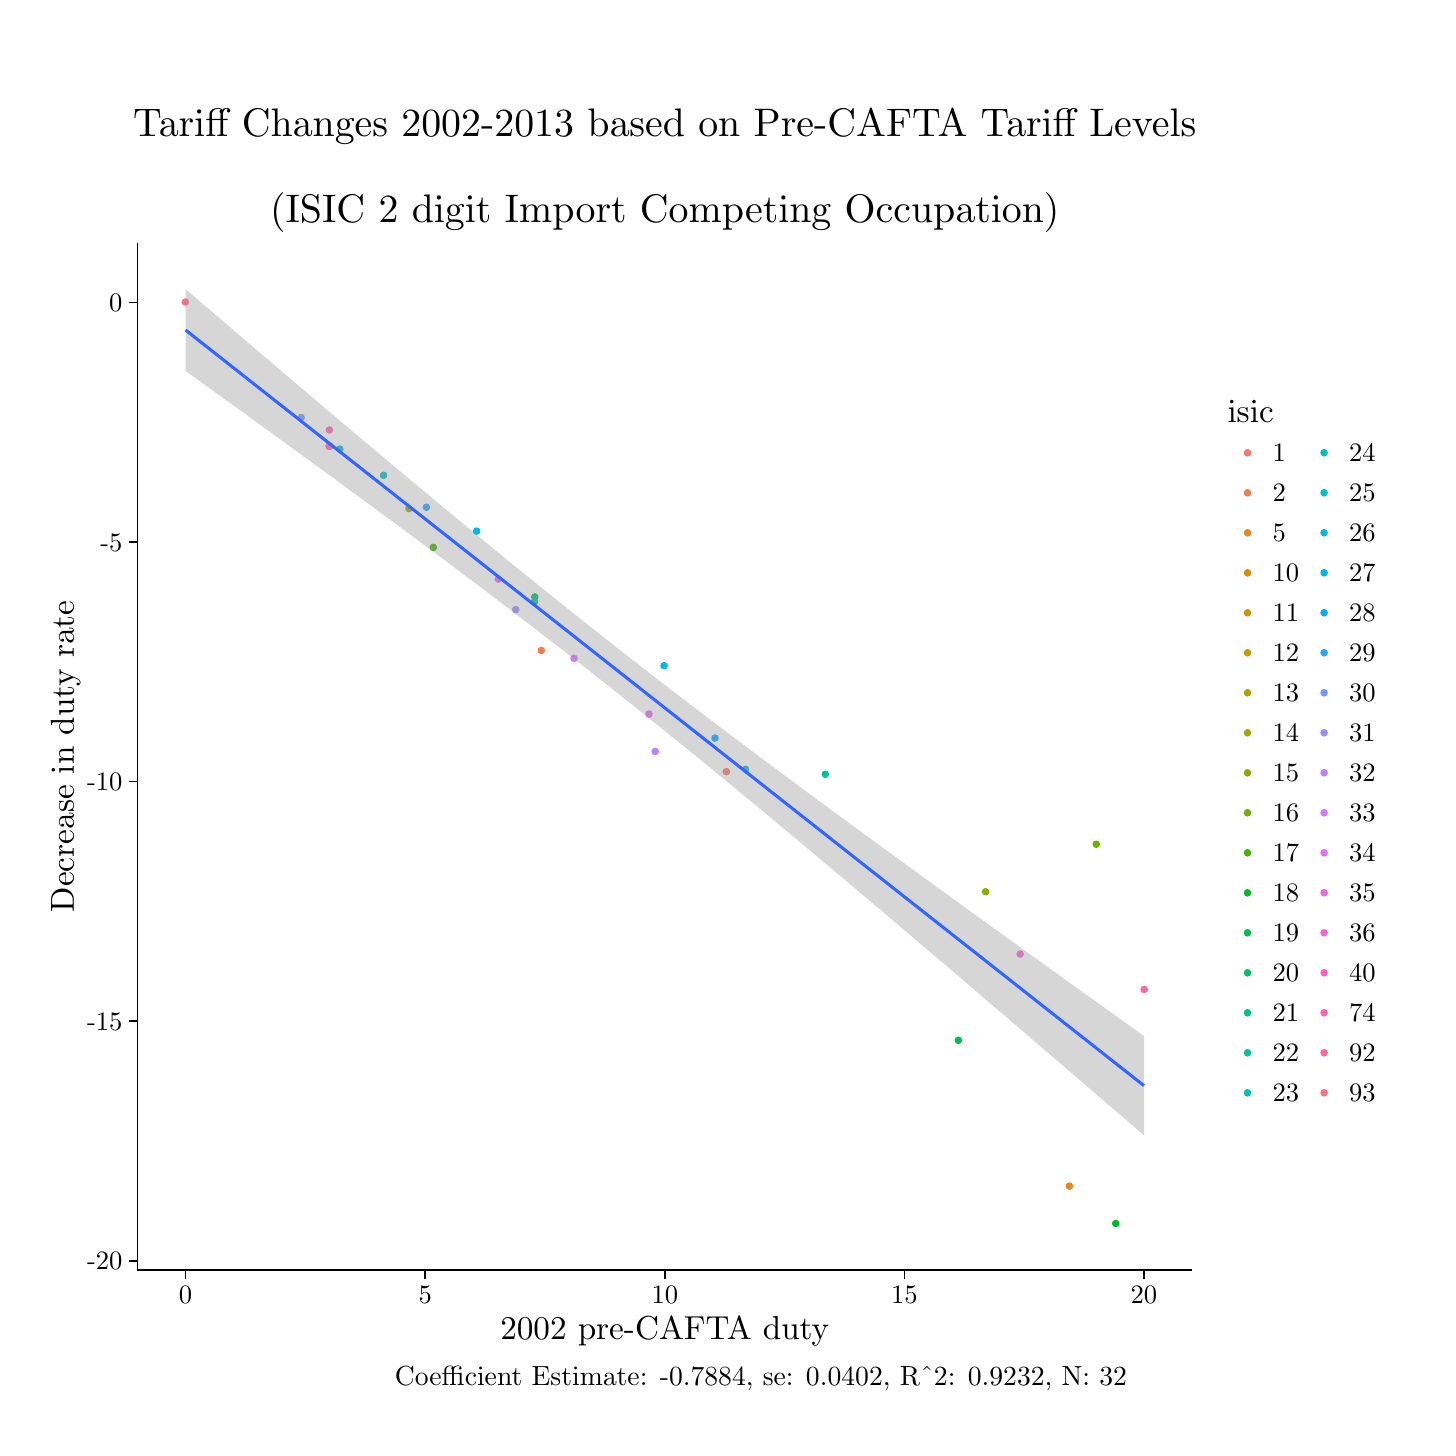
\begin{tikzpicture}[x=1pt,y=1pt]
\definecolor{fillColor}{RGB}{255,255,255}
\path[use as bounding box,fill=fillColor,fill opacity=0.00] (0,0) rectangle (505.89,505.89);
\begin{scope}
\path[clip] (  0.00, 23.42) rectangle (505.89,482.47);
\definecolor{drawColor}{RGB}{255,255,255}
\definecolor{fillColor}{RGB}{255,255,255}

\path[draw=drawColor,line width= 0.6pt,line join=round,line cap=round,fill=fillColor] (  0.00, 23.42) rectangle (505.89,482.47);
\end{scope}
\begin{scope}
\path[clip] ( 39.66, 56.90) rectangle (420.76,428.25);
\definecolor{fillColor}{RGB}{255,255,255}

\path[fill=fillColor] ( 39.66, 56.90) rectangle (420.76,428.25);
\definecolor{drawColor}{RGB}{248,118,109}
\definecolor{fillColor}{RGB}{248,118,109}

\path[draw=drawColor,line width= 0.4pt,line join=round,line cap=round,fill=fillColor] (252.47,237.06) circle (  1.16);
\definecolor{drawColor}{RGB}{221,141,0}
\definecolor{fillColor}{RGB}{221,141,0}

\path[draw=drawColor,line width= 0.4pt,line join=round,line cap=round,fill=fillColor] (109.08,354.75) circle (  1.16);
\definecolor{drawColor}{RGB}{208,148,0}
\definecolor{fillColor}{RGB}{208,148,0}

\path[draw=drawColor,line width= 0.4pt,line join=round,line cap=round,fill=fillColor] (108.98,354.72) circle (  1.16);
\definecolor{drawColor}{RGB}{194,155,0}
\definecolor{fillColor}{RGB}{194,155,0}

\path[draw=drawColor,line width= 0.4pt,line join=round,line cap=round,fill=fillColor] (109.10,354.70) circle (  1.16);
\definecolor{drawColor}{RGB}{178,161,0}
\definecolor{fillColor}{RGB}{178,161,0}

\path[draw=drawColor,line width= 0.4pt,line join=round,line cap=round,fill=fillColor] (108.97,354.66) circle (  1.16);
\definecolor{drawColor}{RGB}{159,167,0}
\definecolor{fillColor}{RGB}{159,167,0}

\path[draw=drawColor,line width= 0.4pt,line join=round,line cap=round,fill=fillColor] (137.75,332.10) circle (  1.16);
\definecolor{drawColor}{RGB}{137,172,0}
\definecolor{fillColor}{RGB}{137,172,0}

\path[draw=drawColor,line width= 0.4pt,line join=round,line cap=round,fill=fillColor] (346.14,193.65) circle (  1.16);
\definecolor{drawColor}{RGB}{109,177,0}
\definecolor{fillColor}{RGB}{109,177,0}

\path[draw=drawColor,line width= 0.4pt,line join=round,line cap=round,fill=fillColor] (386.13,210.82) circle (  1.16);
\definecolor{drawColor}{RGB}{69,181,0}
\definecolor{fillColor}{RGB}{69,181,0}

\path[draw=drawColor,line width= 0.4pt,line join=round,line cap=round,fill=fillColor] (146.58,318.08) circle (  1.16);
\definecolor{drawColor}{RGB}{0,185,39}
\definecolor{fillColor}{RGB}{0,185,39}

\path[draw=drawColor,line width= 0.4pt,line join=round,line cap=round,fill=fillColor] (393.17, 73.78) circle (  1.16);
\definecolor{drawColor}{RGB}{0,188,81}
\definecolor{fillColor}{RGB}{0,188,81}

\path[draw=drawColor,line width= 0.4pt,line join=round,line cap=round,fill=fillColor] (336.29,139.97) circle (  1.16);
\definecolor{drawColor}{RGB}{240,126,78}
\definecolor{fillColor}{RGB}{240,126,78}

\path[draw=drawColor,line width= 0.4pt,line join=round,line cap=round,fill=fillColor] (185.58,280.83) circle (  1.16);
\definecolor{drawColor}{RGB}{0,190,110}
\definecolor{fillColor}{RGB}{0,190,110}

\path[draw=drawColor,line width= 0.4pt,line join=round,line cap=round,fill=fillColor] (183.25,300.19) circle (  1.16);
\definecolor{drawColor}{RGB}{0,192,135}
\definecolor{fillColor}{RGB}{0,192,135}

\path[draw=drawColor,line width= 0.4pt,line join=round,line cap=round,fill=fillColor] (183.10,298.45) circle (  1.16);
\definecolor{drawColor}{RGB}{0,193,157}
\definecolor{fillColor}{RGB}{0,193,157}

\path[draw=drawColor,line width= 0.4pt,line join=round,line cap=round,fill=fillColor] (288.23,236.12) circle (  1.16);
\definecolor{drawColor}{RGB}{0,192,178}
\definecolor{fillColor}{RGB}{0,192,178}

\path[draw=drawColor,line width= 0.4pt,line join=round,line cap=round,fill=fillColor] (112.78,353.62) circle (  1.16);
\definecolor{drawColor}{RGB}{0,191,196}
\definecolor{fillColor}{RGB}{0,191,196}

\path[draw=drawColor,line width= 0.4pt,line join=round,line cap=round,fill=fillColor] (128.59,344.12) circle (  1.16);
\definecolor{drawColor}{RGB}{0,188,214}
\definecolor{fillColor}{RGB}{0,188,214}

\path[draw=drawColor,line width= 0.4pt,line join=round,line cap=round,fill=fillColor] (259.39,237.91) circle (  1.16);
\definecolor{drawColor}{RGB}{0,184,229}
\definecolor{fillColor}{RGB}{0,184,229}

\path[draw=drawColor,line width= 0.4pt,line join=round,line cap=round,fill=fillColor] (229.97,275.34) circle (  1.16);
\definecolor{drawColor}{RGB}{0,179,242}
\definecolor{fillColor}{RGB}{0,179,242}

\path[draw=drawColor,line width= 0.4pt,line join=round,line cap=round,fill=fillColor] (162.23,323.95) circle (  1.16);
\definecolor{drawColor}{RGB}{0,171,252}
\definecolor{fillColor}{RGB}{0,171,252}

\path[draw=drawColor,line width= 0.4pt,line join=round,line cap=round,fill=fillColor] (248.37,249.19) circle (  1.16);
\definecolor{drawColor}{RGB}{41,163,255}
\definecolor{fillColor}{RGB}{41,163,255}

\path[draw=drawColor,line width= 0.4pt,line join=round,line cap=round,fill=fillColor] (144.06,332.60) circle (  1.16);
\definecolor{drawColor}{RGB}{115,152,255}
\definecolor{fillColor}{RGB}{115,152,255}

\path[draw=drawColor,line width= 0.4pt,line join=round,line cap=round,fill=fillColor] ( 98.82,365.01) circle (  1.16);
\definecolor{drawColor}{RGB}{156,141,255}
\definecolor{fillColor}{RGB}{156,141,255}

\path[draw=drawColor,line width= 0.4pt,line join=round,line cap=round,fill=fillColor] (176.37,295.58) circle (  1.16);
\definecolor{drawColor}{RGB}{186,130,255}
\definecolor{fillColor}{RGB}{186,130,255}

\path[draw=drawColor,line width= 0.4pt,line join=round,line cap=round,fill=fillColor] (226.74,244.36) circle (  1.16);
\definecolor{drawColor}{RGB}{210,119,255}
\definecolor{fillColor}{RGB}{210,119,255}

\path[draw=drawColor,line width= 0.4pt,line join=round,line cap=round,fill=fillColor] (197.44,277.98) circle (  1.16);
\definecolor{drawColor}{RGB}{228,109,245}
\definecolor{fillColor}{RGB}{228,109,245}

\path[draw=drawColor,line width= 0.4pt,line join=round,line cap=round,fill=fillColor] (224.49,257.85) circle (  1.16);
\definecolor{drawColor}{RGB}{241,102,232}
\definecolor{fillColor}{RGB}{241,102,232}

\path[draw=drawColor,line width= 0.4pt,line join=round,line cap=round,fill=fillColor] (170.09,306.63) circle (  1.16);
\definecolor{drawColor}{RGB}{250,98,217}
\definecolor{fillColor}{RGB}{250,98,217}

\path[draw=drawColor,line width= 0.4pt,line join=round,line cap=round,fill=fillColor] (358.63,171.13) circle (  1.16);
\definecolor{drawColor}{RGB}{255,97,199}
\definecolor{fillColor}{RGB}{255,97,199}

\path[draw=drawColor,line width= 0.4pt,line join=round,line cap=round,fill=fillColor] (109.00,354.58) circle (  1.16);
\definecolor{drawColor}{RGB}{231,133,30}
\definecolor{fillColor}{RGB}{231,133,30}

\path[draw=drawColor,line width= 0.4pt,line join=round,line cap=round,fill=fillColor] (376.42, 87.26) circle (  1.16);
\definecolor{drawColor}{RGB}{255,99,180}
\definecolor{fillColor}{RGB}{255,99,180}

\path[draw=drawColor,line width= 0.4pt,line join=round,line cap=round,fill=fillColor] (109.04,360.52) circle (  1.16);
\definecolor{drawColor}{RGB}{255,104,158}
\definecolor{fillColor}{RGB}{255,104,158}

\path[draw=drawColor,line width= 0.4pt,line join=round,line cap=round,fill=fillColor] (403.44,158.34) circle (  1.16);
\definecolor{drawColor}{RGB}{253,111,135}
\definecolor{fillColor}{RGB}{253,111,135}

\path[draw=drawColor,line width= 0.4pt,line join=round,line cap=round,fill=fillColor] ( 56.98,406.74) circle (  1.16);
\definecolor{fillColor}{RGB}{153,153,153}

\path[fill=fillColor,fill opacity=0.40] ( 57.08,411.37) --
	( 61.46,407.61) --
	( 65.85,403.86) --
	( 70.23,400.11) --
	( 74.61,396.37) --
	( 79.00,392.62) --
	( 83.38,388.88) --
	( 87.76,385.15) --
	( 92.15,381.42) --
	( 96.53,377.69) --
	(100.91,373.97) --
	(105.30,370.25) --
	(109.68,366.54) --
	(114.06,362.83) --
	(118.45,359.13) --
	(122.83,355.44) --
	(127.22,351.75) --
	(131.60,348.08) --
	(135.98,344.40) --
	(140.37,340.74) --
	(144.75,337.09) --
	(149.13,333.44) --
	(153.52,329.81) --
	(157.90,326.19) --
	(162.28,322.57) --
	(166.67,318.97) --
	(171.05,315.39) --
	(175.43,311.81) --
	(179.82,308.25) --
	(184.20,304.70) --
	(188.58,301.17) --
	(192.97,297.65) --
	(197.35,294.15) --
	(201.73,290.67) --
	(206.12,287.20) --
	(210.50,283.74) --
	(214.89,280.30) --
	(219.27,276.88) --
	(223.65,273.47) --
	(228.04,270.08) --
	(232.42,266.70) --
	(236.80,263.34) --
	(241.19,259.99) --
	(245.57,256.66) --
	(249.95,253.34) --
	(254.34,250.03) --
	(258.72,246.73) --
	(263.10,243.44) --
	(267.49,240.17) --
	(271.87,236.90) --
	(276.25,233.65) --
	(280.64,230.40) --
	(285.02,227.16) --
	(289.40,223.93) --
	(293.79,220.70) --
	(298.17,217.49) --
	(302.55,214.28) --
	(306.94,211.07) --
	(311.32,207.87) --
	(315.71,204.68) --
	(320.09,201.49) --
	(324.47,198.30) --
	(328.86,195.12) --
	(333.24,191.95) --
	(337.62,188.77) --
	(342.01,185.61) --
	(346.39,182.44) --
	(350.77,179.28) --
	(355.16,176.12) --
	(359.54,172.96) --
	(363.92,169.81) --
	(368.31,166.66) --
	(372.69,163.51) --
	(377.07,160.36) --
	(381.46,157.21) --
	(385.84,154.07) --
	(390.22,150.93) --
	(394.61,147.79) --
	(398.99,144.65) --
	(403.38,141.52) --
	(403.38,105.63) --
	(398.99,109.41) --
	(394.61,113.18) --
	(390.22,116.95) --
	(385.84,120.72) --
	(381.46,124.49) --
	(377.07,128.26) --
	(372.69,132.02) --
	(368.31,135.79) --
	(363.92,139.55) --
	(359.54,143.30) --
	(355.16,147.06) --
	(350.77,150.81) --
	(346.39,154.56) --
	(342.01,158.31) --
	(337.62,162.05) --
	(333.24,165.79) --
	(328.86,169.53) --
	(324.47,173.26) --
	(320.09,176.99) --
	(315.71,180.71) --
	(311.32,184.43) --
	(306.94,188.14) --
	(302.55,191.85) --
	(298.17,195.55) --
	(293.79,199.24) --
	(289.40,202.93) --
	(285.02,206.61) --
	(280.64,210.29) --
	(276.25,213.95) --
	(271.87,217.61) --
	(267.49,221.25) --
	(263.10,224.89) --
	(258.72,228.51) --
	(254.34,232.13) --
	(249.95,235.73) --
	(245.57,239.32) --
	(241.19,242.90) --
	(236.80,246.46) --
	(232.42,250.01) --
	(228.04,253.55) --
	(223.65,257.07) --
	(219.27,260.57) --
	(214.89,264.06) --
	(210.50,267.54) --
	(206.12,270.99) --
	(201.73,274.44) --
	(197.35,277.86) --
	(192.97,281.27) --
	(188.58,284.67) --
	(184.20,288.05) --
	(179.82,291.41) --
	(175.43,294.76) --
	(171.05,298.10) --
	(166.67,301.43) --
	(162.28,304.74) --
	(157.90,308.04) --
	(153.52,311.33) --
	(149.13,314.60) --
	(144.75,317.87) --
	(140.37,321.13) --
	(135.98,324.38) --
	(131.60,327.62) --
	(127.22,330.85) --
	(122.83,334.08) --
	(118.45,337.30) --
	(114.06,340.51) --
	(109.68,343.72) --
	(105.30,346.92) --
	(100.91,350.11) --
	( 96.53,353.30) --
	( 92.15,356.49) --
	( 87.76,359.67) --
	( 83.38,362.84) --
	( 79.00,366.02) --
	( 74.61,369.19) --
	( 70.23,372.35) --
	( 65.85,375.52) --
	( 61.46,378.68) --
	( 57.08,381.83) --
	cycle;
\definecolor{drawColor}{RGB}{51,102,255}

\path[draw=drawColor,line width= 1.1pt,line join=round] ( 57.08,396.60) --
	( 61.46,393.14) --
	( 65.85,389.69) --
	( 70.23,386.23) --
	( 74.61,382.78) --
	( 79.00,379.32) --
	( 83.38,375.86) --
	( 87.76,372.41) --
	( 92.15,368.95) --
	( 96.53,365.50) --
	(100.91,362.04) --
	(105.30,358.58) --
	(109.68,355.13) --
	(114.06,351.67) --
	(118.45,348.22) --
	(122.83,344.76) --
	(127.22,341.30) --
	(131.60,337.85) --
	(135.98,334.39) --
	(140.37,330.94) --
	(144.75,327.48) --
	(149.13,324.02) --
	(153.52,320.57) --
	(157.90,317.11) --
	(162.28,313.66) --
	(166.67,310.20) --
	(171.05,306.74) --
	(175.43,303.29) --
	(179.82,299.83) --
	(184.20,296.38) --
	(188.58,292.92) --
	(192.97,289.46) --
	(197.35,286.01) --
	(201.73,282.55) --
	(206.12,279.10) --
	(210.50,275.64) --
	(214.89,272.18) --
	(219.27,268.73) --
	(223.65,265.27) --
	(228.04,261.81) --
	(232.42,258.36) --
	(236.80,254.90) --
	(241.19,251.45) --
	(245.57,247.99) --
	(249.95,244.53) --
	(254.34,241.08) --
	(258.72,237.62) --
	(263.10,234.17) --
	(267.49,230.71) --
	(271.87,227.25) --
	(276.25,223.80) --
	(280.64,220.34) --
	(285.02,216.89) --
	(289.40,213.43) --
	(293.79,209.97) --
	(298.17,206.52) --
	(302.55,203.06) --
	(306.94,199.61) --
	(311.32,196.15) --
	(315.71,192.69) --
	(320.09,189.24) --
	(324.47,185.78) --
	(328.86,182.33) --
	(333.24,178.87) --
	(337.62,175.41) --
	(342.01,171.96) --
	(346.39,168.50) --
	(350.77,165.05) --
	(355.16,161.59) --
	(359.54,158.13) --
	(363.92,154.68) --
	(368.31,151.22) --
	(372.69,147.77) --
	(377.07,144.31) --
	(381.46,140.85) --
	(385.84,137.40) --
	(390.22,133.94) --
	(394.61,130.48) --
	(398.99,127.03) --
	(403.38,123.57);
\end{scope}
\begin{scope}
\path[clip] (  0.00,  0.00) rectangle (505.89,505.89);
\definecolor{drawColor}{RGB}{0,0,0}

\path[draw=drawColor,line width= 0.6pt,line join=round] ( 39.66, 56.90) --
	( 39.66,428.25);
\end{scope}
\begin{scope}
\path[clip] (  0.00,  0.00) rectangle (505.89,505.89);
\definecolor{drawColor}{RGB}{0,0,0}

\node[text=drawColor,anchor=base east,inner sep=0pt, outer sep=0pt, scale=  0.96] at ( 34.26, 57.03) {-20};

\node[text=drawColor,anchor=base east,inner sep=0pt, outer sep=0pt, scale=  0.96] at ( 34.26,143.60) {-15};

\node[text=drawColor,anchor=base east,inner sep=0pt, outer sep=0pt, scale=  0.96] at ( 34.26,230.18) {-10};

\node[text=drawColor,anchor=base east,inner sep=0pt, outer sep=0pt, scale=  0.96] at ( 34.26,316.75) {-5};

\node[text=drawColor,anchor=base east,inner sep=0pt, outer sep=0pt, scale=  0.96] at ( 34.26,403.33) {0};
\end{scope}
\begin{scope}
\path[clip] (  0.00,  0.00) rectangle (505.89,505.89);
\definecolor{drawColor}{RGB}{0,0,0}

\path[draw=drawColor,line width= 0.6pt,line join=round] ( 36.66, 60.34) --
	( 39.66, 60.34);

\path[draw=drawColor,line width= 0.6pt,line join=round] ( 36.66,146.91) --
	( 39.66,146.91);

\path[draw=drawColor,line width= 0.6pt,line join=round] ( 36.66,233.48) --
	( 39.66,233.48);

\path[draw=drawColor,line width= 0.6pt,line join=round] ( 36.66,320.06) --
	( 39.66,320.06);

\path[draw=drawColor,line width= 0.6pt,line join=round] ( 36.66,406.63) --
	( 39.66,406.63);
\end{scope}
\begin{scope}
\path[clip] (  0.00,  0.00) rectangle (505.89,505.89);
\definecolor{drawColor}{RGB}{0,0,0}

\path[draw=drawColor,line width= 0.6pt,line join=round] ( 39.66, 56.90) --
	(420.76, 56.90);
\end{scope}
\begin{scope}
\path[clip] (  0.00,  0.00) rectangle (505.89,505.89);
\definecolor{drawColor}{RGB}{0,0,0}

\path[draw=drawColor,line width= 0.6pt,line join=round] ( 57.08, 53.90) --
	( 57.08, 56.90);

\path[draw=drawColor,line width= 0.6pt,line join=round] (143.65, 53.90) --
	(143.65, 56.90);

\path[draw=drawColor,line width= 0.6pt,line join=round] (230.23, 53.90) --
	(230.23, 56.90);

\path[draw=drawColor,line width= 0.6pt,line join=round] (316.80, 53.90) --
	(316.80, 56.90);

\path[draw=drawColor,line width= 0.6pt,line join=round] (403.38, 53.90) --
	(403.38, 56.90);
\end{scope}
\begin{scope}
\path[clip] (  0.00,  0.00) rectangle (505.89,505.89);
\definecolor{drawColor}{RGB}{0,0,0}

\node[text=drawColor,anchor=base,inner sep=0pt, outer sep=0pt, scale=  0.96] at ( 57.08, 44.89) {0};

\node[text=drawColor,anchor=base,inner sep=0pt, outer sep=0pt, scale=  0.96] at (143.65, 44.89) {5};

\node[text=drawColor,anchor=base,inner sep=0pt, outer sep=0pt, scale=  0.96] at (230.23, 44.89) {10};

\node[text=drawColor,anchor=base,inner sep=0pt, outer sep=0pt, scale=  0.96] at (316.80, 44.89) {15};

\node[text=drawColor,anchor=base,inner sep=0pt, outer sep=0pt, scale=  0.96] at (403.38, 44.89) {20};
\end{scope}
\begin{scope}
\path[clip] (  0.00,  0.00) rectangle (505.89,505.89);
\definecolor{drawColor}{RGB}{0,0,0}

\node[text=drawColor,anchor=base,inner sep=0pt, outer sep=0pt, scale=  1.20] at (230.21, 31.82) {2002 pre-CAFTA duty};
\end{scope}
\begin{scope}
\path[clip] (  0.00,  0.00) rectangle (505.89,505.89);
\definecolor{drawColor}{RGB}{0,0,0}

\node[text=drawColor,rotate= 90.00,anchor=base,inner sep=0pt, outer sep=0pt, scale=  1.20] at ( 16.66,242.57) {Decrease in duty rate};
\end{scope}
\begin{scope}
\path[clip] (  0.00,  0.00) rectangle (505.89,505.89);
\definecolor{fillColor}{RGB}{255,255,255}

\path[fill=fillColor] (429.29,109.51) rectangle (491.35,375.64);
\end{scope}
\begin{scope}
\path[clip] (  0.00,  0.00) rectangle (505.89,505.89);
\definecolor{drawColor}{RGB}{0,0,0}

\node[text=drawColor,anchor=base west,inner sep=0pt, outer sep=0pt, scale=  1.20] at (433.56,363.11) {isic};
\end{scope}
\begin{scope}
\path[clip] (  0.00,  0.00) rectangle (505.89,505.89);
\definecolor{drawColor}{RGB}{248,118,109}
\definecolor{fillColor}{RGB}{248,118,109}

\path[draw=drawColor,line width= 0.4pt,line join=round,line cap=round,fill=fillColor] (440.79,352.27) circle (  1.16);
\end{scope}
\begin{scope}
\path[clip] (  0.00,  0.00) rectangle (505.89,505.89);
\definecolor{drawColor}{RGB}{240,126,78}
\definecolor{fillColor}{RGB}{240,126,78}

\path[draw=drawColor,line width= 0.4pt,line join=round,line cap=round,fill=fillColor] (440.79,337.81) circle (  1.16);
\end{scope}
\begin{scope}
\path[clip] (  0.00,  0.00) rectangle (505.89,505.89);
\definecolor{drawColor}{RGB}{231,133,30}
\definecolor{fillColor}{RGB}{231,133,30}

\path[draw=drawColor,line width= 0.4pt,line join=round,line cap=round,fill=fillColor] (440.79,323.36) circle (  1.16);
\end{scope}
\begin{scope}
\path[clip] (  0.00,  0.00) rectangle (505.89,505.89);
\definecolor{drawColor}{RGB}{221,141,0}
\definecolor{fillColor}{RGB}{221,141,0}

\path[draw=drawColor,line width= 0.4pt,line join=round,line cap=round,fill=fillColor] (440.79,308.90) circle (  1.16);
\end{scope}
\begin{scope}
\path[clip] (  0.00,  0.00) rectangle (505.89,505.89);
\definecolor{drawColor}{RGB}{208,148,0}
\definecolor{fillColor}{RGB}{208,148,0}

\path[draw=drawColor,line width= 0.4pt,line join=round,line cap=round,fill=fillColor] (440.79,294.45) circle (  1.16);
\end{scope}
\begin{scope}
\path[clip] (  0.00,  0.00) rectangle (505.89,505.89);
\definecolor{drawColor}{RGB}{194,155,0}
\definecolor{fillColor}{RGB}{194,155,0}

\path[draw=drawColor,line width= 0.4pt,line join=round,line cap=round,fill=fillColor] (440.79,280.00) circle (  1.16);
\end{scope}
\begin{scope}
\path[clip] (  0.00,  0.00) rectangle (505.89,505.89);
\definecolor{drawColor}{RGB}{178,161,0}
\definecolor{fillColor}{RGB}{178,161,0}

\path[draw=drawColor,line width= 0.4pt,line join=round,line cap=round,fill=fillColor] (440.79,265.54) circle (  1.16);
\end{scope}
\begin{scope}
\path[clip] (  0.00,  0.00) rectangle (505.89,505.89);
\definecolor{drawColor}{RGB}{159,167,0}
\definecolor{fillColor}{RGB}{159,167,0}

\path[draw=drawColor,line width= 0.4pt,line join=round,line cap=round,fill=fillColor] (440.79,251.09) circle (  1.16);
\end{scope}
\begin{scope}
\path[clip] (  0.00,  0.00) rectangle (505.89,505.89);
\definecolor{drawColor}{RGB}{137,172,0}
\definecolor{fillColor}{RGB}{137,172,0}

\path[draw=drawColor,line width= 0.4pt,line join=round,line cap=round,fill=fillColor] (440.79,236.63) circle (  1.16);
\end{scope}
\begin{scope}
\path[clip] (  0.00,  0.00) rectangle (505.89,505.89);
\definecolor{drawColor}{RGB}{109,177,0}
\definecolor{fillColor}{RGB}{109,177,0}

\path[draw=drawColor,line width= 0.4pt,line join=round,line cap=round,fill=fillColor] (440.79,222.18) circle (  1.16);
\end{scope}
\begin{scope}
\path[clip] (  0.00,  0.00) rectangle (505.89,505.89);
\definecolor{drawColor}{RGB}{69,181,0}
\definecolor{fillColor}{RGB}{69,181,0}

\path[draw=drawColor,line width= 0.4pt,line join=round,line cap=round,fill=fillColor] (440.79,207.73) circle (  1.16);
\end{scope}
\begin{scope}
\path[clip] (  0.00,  0.00) rectangle (505.89,505.89);
\definecolor{drawColor}{RGB}{0,185,39}
\definecolor{fillColor}{RGB}{0,185,39}

\path[draw=drawColor,line width= 0.4pt,line join=round,line cap=round,fill=fillColor] (440.79,193.27) circle (  1.16);
\end{scope}
\begin{scope}
\path[clip] (  0.00,  0.00) rectangle (505.89,505.89);
\definecolor{drawColor}{RGB}{0,188,81}
\definecolor{fillColor}{RGB}{0,188,81}

\path[draw=drawColor,line width= 0.4pt,line join=round,line cap=round,fill=fillColor] (440.79,178.82) circle (  1.16);
\end{scope}
\begin{scope}
\path[clip] (  0.00,  0.00) rectangle (505.89,505.89);
\definecolor{drawColor}{RGB}{0,190,110}
\definecolor{fillColor}{RGB}{0,190,110}

\path[draw=drawColor,line width= 0.4pt,line join=round,line cap=round,fill=fillColor] (440.79,164.36) circle (  1.16);
\end{scope}
\begin{scope}
\path[clip] (  0.00,  0.00) rectangle (505.89,505.89);
\definecolor{drawColor}{RGB}{0,192,135}
\definecolor{fillColor}{RGB}{0,192,135}

\path[draw=drawColor,line width= 0.4pt,line join=round,line cap=round,fill=fillColor] (440.79,149.91) circle (  1.16);
\end{scope}
\begin{scope}
\path[clip] (  0.00,  0.00) rectangle (505.89,505.89);
\definecolor{drawColor}{RGB}{0,193,157}
\definecolor{fillColor}{RGB}{0,193,157}

\path[draw=drawColor,line width= 0.4pt,line join=round,line cap=round,fill=fillColor] (440.79,135.46) circle (  1.16);
\end{scope}
\begin{scope}
\path[clip] (  0.00,  0.00) rectangle (505.89,505.89);
\definecolor{drawColor}{RGB}{0,192,178}
\definecolor{fillColor}{RGB}{0,192,178}

\path[draw=drawColor,line width= 0.4pt,line join=round,line cap=round,fill=fillColor] (440.79,121.00) circle (  1.16);
\end{scope}
\begin{scope}
\path[clip] (  0.00,  0.00) rectangle (505.89,505.89);
\definecolor{drawColor}{RGB}{0,191,196}
\definecolor{fillColor}{RGB}{0,191,196}

\path[draw=drawColor,line width= 0.4pt,line join=round,line cap=round,fill=fillColor] (468.45,352.27) circle (  1.16);
\end{scope}
\begin{scope}
\path[clip] (  0.00,  0.00) rectangle (505.89,505.89);
\definecolor{drawColor}{RGB}{0,188,214}
\definecolor{fillColor}{RGB}{0,188,214}

\path[draw=drawColor,line width= 0.4pt,line join=round,line cap=round,fill=fillColor] (468.45,337.81) circle (  1.16);
\end{scope}
\begin{scope}
\path[clip] (  0.00,  0.00) rectangle (505.89,505.89);
\definecolor{drawColor}{RGB}{0,184,229}
\definecolor{fillColor}{RGB}{0,184,229}

\path[draw=drawColor,line width= 0.4pt,line join=round,line cap=round,fill=fillColor] (468.45,323.36) circle (  1.16);
\end{scope}
\begin{scope}
\path[clip] (  0.00,  0.00) rectangle (505.89,505.89);
\definecolor{drawColor}{RGB}{0,179,242}
\definecolor{fillColor}{RGB}{0,179,242}

\path[draw=drawColor,line width= 0.4pt,line join=round,line cap=round,fill=fillColor] (468.45,308.90) circle (  1.16);
\end{scope}
\begin{scope}
\path[clip] (  0.00,  0.00) rectangle (505.89,505.89);
\definecolor{drawColor}{RGB}{0,171,252}
\definecolor{fillColor}{RGB}{0,171,252}

\path[draw=drawColor,line width= 0.4pt,line join=round,line cap=round,fill=fillColor] (468.45,294.45) circle (  1.16);
\end{scope}
\begin{scope}
\path[clip] (  0.00,  0.00) rectangle (505.89,505.89);
\definecolor{drawColor}{RGB}{41,163,255}
\definecolor{fillColor}{RGB}{41,163,255}

\path[draw=drawColor,line width= 0.4pt,line join=round,line cap=round,fill=fillColor] (468.45,280.00) circle (  1.16);
\end{scope}
\begin{scope}
\path[clip] (  0.00,  0.00) rectangle (505.89,505.89);
\definecolor{drawColor}{RGB}{115,152,255}
\definecolor{fillColor}{RGB}{115,152,255}

\path[draw=drawColor,line width= 0.4pt,line join=round,line cap=round,fill=fillColor] (468.45,265.54) circle (  1.16);
\end{scope}
\begin{scope}
\path[clip] (  0.00,  0.00) rectangle (505.89,505.89);
\definecolor{drawColor}{RGB}{156,141,255}
\definecolor{fillColor}{RGB}{156,141,255}

\path[draw=drawColor,line width= 0.4pt,line join=round,line cap=round,fill=fillColor] (468.45,251.09) circle (  1.16);
\end{scope}
\begin{scope}
\path[clip] (  0.00,  0.00) rectangle (505.89,505.89);
\definecolor{drawColor}{RGB}{186,130,255}
\definecolor{fillColor}{RGB}{186,130,255}

\path[draw=drawColor,line width= 0.4pt,line join=round,line cap=round,fill=fillColor] (468.45,236.63) circle (  1.16);
\end{scope}
\begin{scope}
\path[clip] (  0.00,  0.00) rectangle (505.89,505.89);
\definecolor{drawColor}{RGB}{210,119,255}
\definecolor{fillColor}{RGB}{210,119,255}

\path[draw=drawColor,line width= 0.4pt,line join=round,line cap=round,fill=fillColor] (468.45,222.18) circle (  1.16);
\end{scope}
\begin{scope}
\path[clip] (  0.00,  0.00) rectangle (505.89,505.89);
\definecolor{drawColor}{RGB}{228,109,245}
\definecolor{fillColor}{RGB}{228,109,245}

\path[draw=drawColor,line width= 0.4pt,line join=round,line cap=round,fill=fillColor] (468.45,207.73) circle (  1.16);
\end{scope}
\begin{scope}
\path[clip] (  0.00,  0.00) rectangle (505.89,505.89);
\definecolor{drawColor}{RGB}{241,102,232}
\definecolor{fillColor}{RGB}{241,102,232}

\path[draw=drawColor,line width= 0.4pt,line join=round,line cap=round,fill=fillColor] (468.45,193.27) circle (  1.16);
\end{scope}
\begin{scope}
\path[clip] (  0.00,  0.00) rectangle (505.89,505.89);
\definecolor{drawColor}{RGB}{250,98,217}
\definecolor{fillColor}{RGB}{250,98,217}

\path[draw=drawColor,line width= 0.4pt,line join=round,line cap=round,fill=fillColor] (468.45,178.82) circle (  1.16);
\end{scope}
\begin{scope}
\path[clip] (  0.00,  0.00) rectangle (505.89,505.89);
\definecolor{drawColor}{RGB}{255,97,199}
\definecolor{fillColor}{RGB}{255,97,199}

\path[draw=drawColor,line width= 0.4pt,line join=round,line cap=round,fill=fillColor] (468.45,164.36) circle (  1.16);
\end{scope}
\begin{scope}
\path[clip] (  0.00,  0.00) rectangle (505.89,505.89);
\definecolor{drawColor}{RGB}{255,99,180}
\definecolor{fillColor}{RGB}{255,99,180}

\path[draw=drawColor,line width= 0.4pt,line join=round,line cap=round,fill=fillColor] (468.45,149.91) circle (  1.16);
\end{scope}
\begin{scope}
\path[clip] (  0.00,  0.00) rectangle (505.89,505.89);
\definecolor{drawColor}{RGB}{255,104,158}
\definecolor{fillColor}{RGB}{255,104,158}

\path[draw=drawColor,line width= 0.4pt,line join=round,line cap=round,fill=fillColor] (468.45,135.46) circle (  1.16);
\end{scope}
\begin{scope}
\path[clip] (  0.00,  0.00) rectangle (505.89,505.89);
\definecolor{drawColor}{RGB}{253,111,135}
\definecolor{fillColor}{RGB}{253,111,135}

\path[draw=drawColor,line width= 0.4pt,line join=round,line cap=round,fill=fillColor] (468.45,121.00) circle (  1.16);
\end{scope}
\begin{scope}
\path[clip] (  0.00,  0.00) rectangle (505.89,505.89);
\definecolor{drawColor}{RGB}{0,0,0}

\node[text=drawColor,anchor=base west,inner sep=0pt, outer sep=0pt, scale=  0.96] at (449.82,348.96) {1};
\end{scope}
\begin{scope}
\path[clip] (  0.00,  0.00) rectangle (505.89,505.89);
\definecolor{drawColor}{RGB}{0,0,0}

\node[text=drawColor,anchor=base west,inner sep=0pt, outer sep=0pt, scale=  0.96] at (449.82,334.51) {2};
\end{scope}
\begin{scope}
\path[clip] (  0.00,  0.00) rectangle (505.89,505.89);
\definecolor{drawColor}{RGB}{0,0,0}

\node[text=drawColor,anchor=base west,inner sep=0pt, outer sep=0pt, scale=  0.96] at (449.82,320.05) {5};
\end{scope}
\begin{scope}
\path[clip] (  0.00,  0.00) rectangle (505.89,505.89);
\definecolor{drawColor}{RGB}{0,0,0}

\node[text=drawColor,anchor=base west,inner sep=0pt, outer sep=0pt, scale=  0.96] at (449.82,305.60) {10};
\end{scope}
\begin{scope}
\path[clip] (  0.00,  0.00) rectangle (505.89,505.89);
\definecolor{drawColor}{RGB}{0,0,0}

\node[text=drawColor,anchor=base west,inner sep=0pt, outer sep=0pt, scale=  0.96] at (449.82,291.14) {11};
\end{scope}
\begin{scope}
\path[clip] (  0.00,  0.00) rectangle (505.89,505.89);
\definecolor{drawColor}{RGB}{0,0,0}

\node[text=drawColor,anchor=base west,inner sep=0pt, outer sep=0pt, scale=  0.96] at (449.82,276.69) {12};
\end{scope}
\begin{scope}
\path[clip] (  0.00,  0.00) rectangle (505.89,505.89);
\definecolor{drawColor}{RGB}{0,0,0}

\node[text=drawColor,anchor=base west,inner sep=0pt, outer sep=0pt, scale=  0.96] at (449.82,262.24) {13};
\end{scope}
\begin{scope}
\path[clip] (  0.00,  0.00) rectangle (505.89,505.89);
\definecolor{drawColor}{RGB}{0,0,0}

\node[text=drawColor,anchor=base west,inner sep=0pt, outer sep=0pt, scale=  0.96] at (449.82,247.78) {14};
\end{scope}
\begin{scope}
\path[clip] (  0.00,  0.00) rectangle (505.89,505.89);
\definecolor{drawColor}{RGB}{0,0,0}

\node[text=drawColor,anchor=base west,inner sep=0pt, outer sep=0pt, scale=  0.96] at (449.82,233.33) {15};
\end{scope}
\begin{scope}
\path[clip] (  0.00,  0.00) rectangle (505.89,505.89);
\definecolor{drawColor}{RGB}{0,0,0}

\node[text=drawColor,anchor=base west,inner sep=0pt, outer sep=0pt, scale=  0.96] at (449.82,218.87) {16};
\end{scope}
\begin{scope}
\path[clip] (  0.00,  0.00) rectangle (505.89,505.89);
\definecolor{drawColor}{RGB}{0,0,0}

\node[text=drawColor,anchor=base west,inner sep=0pt, outer sep=0pt, scale=  0.96] at (449.82,204.42) {17};
\end{scope}
\begin{scope}
\path[clip] (  0.00,  0.00) rectangle (505.89,505.89);
\definecolor{drawColor}{RGB}{0,0,0}

\node[text=drawColor,anchor=base west,inner sep=0pt, outer sep=0pt, scale=  0.96] at (449.82,189.97) {18};
\end{scope}
\begin{scope}
\path[clip] (  0.00,  0.00) rectangle (505.89,505.89);
\definecolor{drawColor}{RGB}{0,0,0}

\node[text=drawColor,anchor=base west,inner sep=0pt, outer sep=0pt, scale=  0.96] at (449.82,175.51) {19};
\end{scope}
\begin{scope}
\path[clip] (  0.00,  0.00) rectangle (505.89,505.89);
\definecolor{drawColor}{RGB}{0,0,0}

\node[text=drawColor,anchor=base west,inner sep=0pt, outer sep=0pt, scale=  0.96] at (449.82,161.06) {20};
\end{scope}
\begin{scope}
\path[clip] (  0.00,  0.00) rectangle (505.89,505.89);
\definecolor{drawColor}{RGB}{0,0,0}

\node[text=drawColor,anchor=base west,inner sep=0pt, outer sep=0pt, scale=  0.96] at (449.82,146.60) {21};
\end{scope}
\begin{scope}
\path[clip] (  0.00,  0.00) rectangle (505.89,505.89);
\definecolor{drawColor}{RGB}{0,0,0}

\node[text=drawColor,anchor=base west,inner sep=0pt, outer sep=0pt, scale=  0.96] at (449.82,132.15) {22};
\end{scope}
\begin{scope}
\path[clip] (  0.00,  0.00) rectangle (505.89,505.89);
\definecolor{drawColor}{RGB}{0,0,0}

\node[text=drawColor,anchor=base west,inner sep=0pt, outer sep=0pt, scale=  0.96] at (449.82,117.70) {23};
\end{scope}
\begin{scope}
\path[clip] (  0.00,  0.00) rectangle (505.89,505.89);
\definecolor{drawColor}{RGB}{0,0,0}

\node[text=drawColor,anchor=base west,inner sep=0pt, outer sep=0pt, scale=  0.96] at (477.49,348.96) {24};
\end{scope}
\begin{scope}
\path[clip] (  0.00,  0.00) rectangle (505.89,505.89);
\definecolor{drawColor}{RGB}{0,0,0}

\node[text=drawColor,anchor=base west,inner sep=0pt, outer sep=0pt, scale=  0.96] at (477.49,334.51) {25};
\end{scope}
\begin{scope}
\path[clip] (  0.00,  0.00) rectangle (505.89,505.89);
\definecolor{drawColor}{RGB}{0,0,0}

\node[text=drawColor,anchor=base west,inner sep=0pt, outer sep=0pt, scale=  0.96] at (477.49,320.05) {26};
\end{scope}
\begin{scope}
\path[clip] (  0.00,  0.00) rectangle (505.89,505.89);
\definecolor{drawColor}{RGB}{0,0,0}

\node[text=drawColor,anchor=base west,inner sep=0pt, outer sep=0pt, scale=  0.96] at (477.49,305.60) {27};
\end{scope}
\begin{scope}
\path[clip] (  0.00,  0.00) rectangle (505.89,505.89);
\definecolor{drawColor}{RGB}{0,0,0}

\node[text=drawColor,anchor=base west,inner sep=0pt, outer sep=0pt, scale=  0.96] at (477.49,291.14) {28};
\end{scope}
\begin{scope}
\path[clip] (  0.00,  0.00) rectangle (505.89,505.89);
\definecolor{drawColor}{RGB}{0,0,0}

\node[text=drawColor,anchor=base west,inner sep=0pt, outer sep=0pt, scale=  0.96] at (477.49,276.69) {29};
\end{scope}
\begin{scope}
\path[clip] (  0.00,  0.00) rectangle (505.89,505.89);
\definecolor{drawColor}{RGB}{0,0,0}

\node[text=drawColor,anchor=base west,inner sep=0pt, outer sep=0pt, scale=  0.96] at (477.49,262.24) {30};
\end{scope}
\begin{scope}
\path[clip] (  0.00,  0.00) rectangle (505.89,505.89);
\definecolor{drawColor}{RGB}{0,0,0}

\node[text=drawColor,anchor=base west,inner sep=0pt, outer sep=0pt, scale=  0.96] at (477.49,247.78) {31};
\end{scope}
\begin{scope}
\path[clip] (  0.00,  0.00) rectangle (505.89,505.89);
\definecolor{drawColor}{RGB}{0,0,0}

\node[text=drawColor,anchor=base west,inner sep=0pt, outer sep=0pt, scale=  0.96] at (477.49,233.33) {32};
\end{scope}
\begin{scope}
\path[clip] (  0.00,  0.00) rectangle (505.89,505.89);
\definecolor{drawColor}{RGB}{0,0,0}

\node[text=drawColor,anchor=base west,inner sep=0pt, outer sep=0pt, scale=  0.96] at (477.49,218.87) {33};
\end{scope}
\begin{scope}
\path[clip] (  0.00,  0.00) rectangle (505.89,505.89);
\definecolor{drawColor}{RGB}{0,0,0}

\node[text=drawColor,anchor=base west,inner sep=0pt, outer sep=0pt, scale=  0.96] at (477.49,204.42) {34};
\end{scope}
\begin{scope}
\path[clip] (  0.00,  0.00) rectangle (505.89,505.89);
\definecolor{drawColor}{RGB}{0,0,0}

\node[text=drawColor,anchor=base west,inner sep=0pt, outer sep=0pt, scale=  0.96] at (477.49,189.97) {35};
\end{scope}
\begin{scope}
\path[clip] (  0.00,  0.00) rectangle (505.89,505.89);
\definecolor{drawColor}{RGB}{0,0,0}

\node[text=drawColor,anchor=base west,inner sep=0pt, outer sep=0pt, scale=  0.96] at (477.49,175.51) {36};
\end{scope}
\begin{scope}
\path[clip] (  0.00,  0.00) rectangle (505.89,505.89);
\definecolor{drawColor}{RGB}{0,0,0}

\node[text=drawColor,anchor=base west,inner sep=0pt, outer sep=0pt, scale=  0.96] at (477.49,161.06) {40};
\end{scope}
\begin{scope}
\path[clip] (  0.00,  0.00) rectangle (505.89,505.89);
\definecolor{drawColor}{RGB}{0,0,0}

\node[text=drawColor,anchor=base west,inner sep=0pt, outer sep=0pt, scale=  0.96] at (477.49,146.60) {74};
\end{scope}
\begin{scope}
\path[clip] (  0.00,  0.00) rectangle (505.89,505.89);
\definecolor{drawColor}{RGB}{0,0,0}

\node[text=drawColor,anchor=base west,inner sep=0pt, outer sep=0pt, scale=  0.96] at (477.49,132.15) {92};
\end{scope}
\begin{scope}
\path[clip] (  0.00,  0.00) rectangle (505.89,505.89);
\definecolor{drawColor}{RGB}{0,0,0}

\node[text=drawColor,anchor=base west,inner sep=0pt, outer sep=0pt, scale=  0.96] at (477.49,117.70) {93};
\end{scope}
\begin{scope}
\path[clip] (  0.00,  0.00) rectangle (505.89,505.89);
\definecolor{drawColor}{RGB}{0,0,0}

\node[text=drawColor,anchor=base,inner sep=0pt, outer sep=0pt, scale=  1.44] at (230.21,466.55) {Tariff Changes 2002-2013 based on Pre-CAFTA Tariff Levels};

\node[text=drawColor,anchor=base,inner sep=0pt, outer sep=0pt, scale=  1.44] at (230.21,451.00) {  };

\node[text=drawColor,anchor=base,inner sep=0pt, outer sep=0pt, scale=  1.44] at (230.21,435.45) {(ISIC 2 digit Import Competing Occupation)};
\end{scope}
\begin{scope}
\path[clip] (  0.00,  0.00) rectangle (505.89,505.89);
\definecolor{drawColor}{RGB}{0,0,0}

\node[text=drawColor,anchor=base,inner sep=0pt, outer sep=0pt, scale=  1.00] at (264.94, 15.09) {Coefficient Estimate: -0.7884, se: 0.0402, R{\^{}}2: 0.9232, N: 32};
\end{scope}
\end{tikzpicture}


\caption{\label{fig:Graph2}}
%Notes: Coefficient Estimate: -0.9326, se: 0.009471, \(R^{2}\) =0.974, N=261
Source: Central American Free Trade Agreement, Office of the United States Trade Representative \&
World Trade Organization, author's calculations
%\end{center}
\end{figure}

\begin{figure}[H]
%\begin{center}
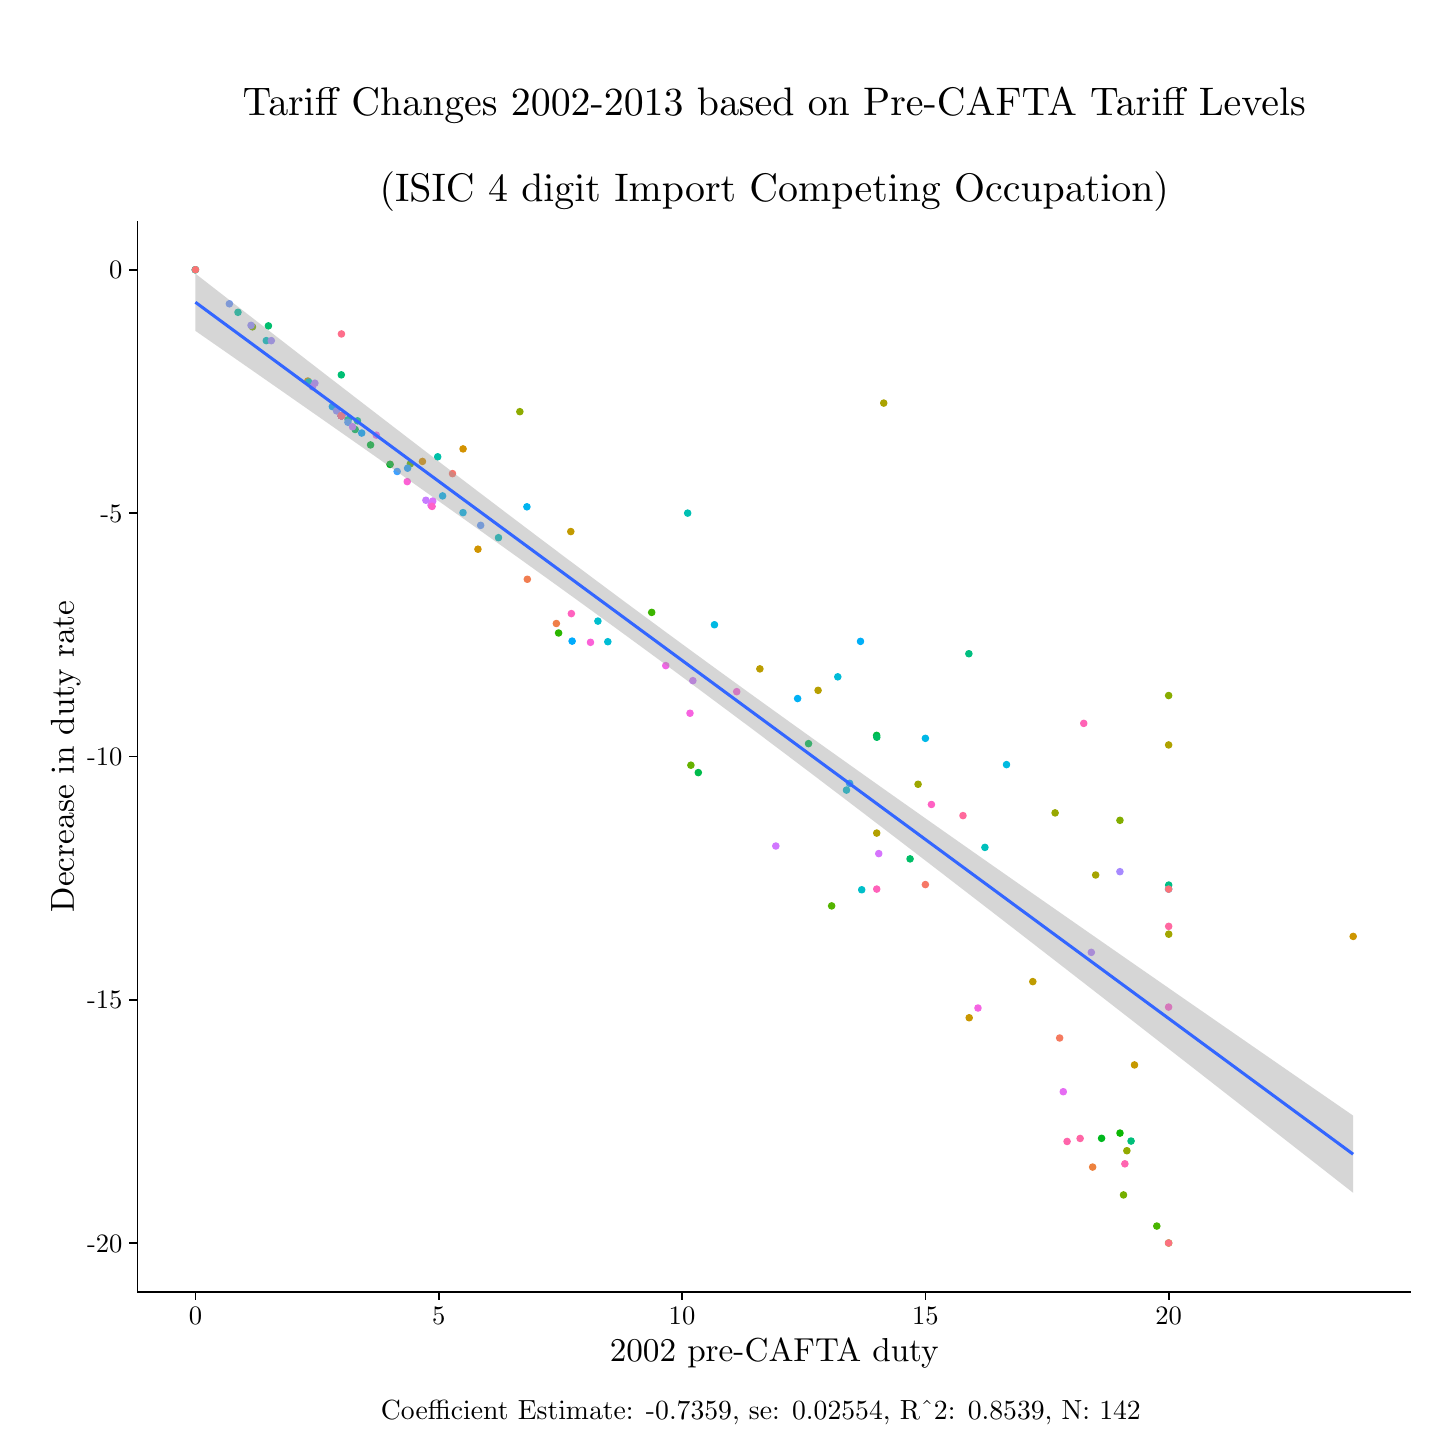
\begin{tikzpicture}[x=1pt,y=1pt]
\definecolor{fillColor}{RGB}{255,255,255}
\path[use as bounding box,fill=fillColor,fill opacity=0.00] (0,0) rectangle (505.89,505.89);
\begin{scope}
\path[clip] (  0.00, 15.67) rectangle (505.89,490.22);
\definecolor{drawColor}{RGB}{255,255,255}
\definecolor{fillColor}{RGB}{255,255,255}

\path[draw=drawColor,line width= 0.6pt,line join=round,line cap=round,fill=fillColor] (  0.00, 15.67) rectangle (505.89,490.22);
\end{scope}
\begin{scope}
\path[clip] ( 39.66, 49.14) rectangle (499.89,436.00);
\definecolor{fillColor}{RGB}{255,255,255}

\path[fill=fillColor] ( 39.66, 49.14) rectangle (499.89,436.00);
\definecolor{drawColor}{RGB}{248,118,109}
\definecolor{fillColor}{RGB}{248,118,109}

\path[draw=drawColor,line width= 0.4pt,line join=round,line cap=round,fill=fillColor] (153.51,344.74) circle (  1.16);
\definecolor{drawColor}{RGB}{246,120,102}
\definecolor{fillColor}{RGB}{246,120,102}

\path[draw=drawColor,line width= 0.4pt,line join=round,line cap=round,fill=fillColor] (324.38,196.24) circle (  1.16);
\definecolor{drawColor}{RGB}{245,122,95}
\definecolor{fillColor}{RGB}{245,122,95}

\path[draw=drawColor,line width= 0.4pt,line join=round,line cap=round,fill=fillColor] (372.90,140.81) circle (  1.16);
\definecolor{drawColor}{RGB}{243,124,88}
\definecolor{fillColor}{RGB}{243,124,88}

\path[draw=drawColor,line width= 0.4pt,line join=round,line cap=round,fill=fillColor] (130.96,348.08) circle (  1.16);
\definecolor{drawColor}{RGB}{241,125,80}
\definecolor{fillColor}{RGB}{241,125,80}

\path[draw=drawColor,line width= 0.4pt,line join=round,line cap=round,fill=fillColor] (180.55,306.57) circle (  1.16);
\definecolor{drawColor}{RGB}{239,127,72}
\definecolor{fillColor}{RGB}{239,127,72}

\path[draw=drawColor,line width= 0.4pt,line join=round,line cap=round,fill=fillColor] (191.04,290.58) circle (  1.16);
\definecolor{drawColor}{RGB}{237,129,62}
\definecolor{fillColor}{RGB}{237,129,62}

\path[draw=drawColor,line width= 0.4pt,line join=round,line cap=round,fill=fillColor] (384.82, 94.17) circle (  1.16);
\definecolor{drawColor}{RGB}{235,131,51}
\definecolor{fillColor}{RGB}{235,131,51}

\path[draw=drawColor,line width= 0.4pt,line join=round,line cap=round,fill=fillColor] (113.35,365.66) circle (  1.16);
\definecolor{drawColor}{RGB}{232,133,38}
\definecolor{fillColor}{RGB}{232,133,38}

\path[draw=drawColor,line width= 0.4pt,line join=round,line cap=round,fill=fillColor] (113.37,365.66) circle (  1.16);
\definecolor{drawColor}{RGB}{230,134,19}
\definecolor{fillColor}{RGB}{230,134,19}

\path[draw=drawColor,line width= 0.4pt,line join=round,line cap=round,fill=fillColor] (113.33,365.66) circle (  1.16);
\definecolor{drawColor}{RGB}{228,136,0}
\definecolor{fillColor}{RGB}{228,136,0}

\path[draw=drawColor,line width= 0.4pt,line join=round,line cap=round,fill=fillColor] (113.34,365.66) circle (  1.16);
\definecolor{drawColor}{RGB}{225,138,0}
\definecolor{fillColor}{RGB}{225,138,0}

\path[draw=drawColor,line width= 0.4pt,line join=round,line cap=round,fill=fillColor] (113.34,365.66) circle (  1.16);
\definecolor{drawColor}{RGB}{222,140,0}
\definecolor{fillColor}{RGB}{222,140,0}

\path[draw=drawColor,line width= 0.4pt,line join=round,line cap=round,fill=fillColor] (113.35,365.66) circle (  1.16);
\definecolor{drawColor}{RGB}{220,141,0}
\definecolor{fillColor}{RGB}{220,141,0}

\path[draw=drawColor,line width= 0.4pt,line join=round,line cap=round,fill=fillColor] (113.35,365.66) circle (  1.16);
\definecolor{drawColor}{RGB}{217,143,0}
\definecolor{fillColor}{RGB}{217,143,0}

\path[draw=drawColor,line width= 0.4pt,line join=round,line cap=round,fill=fillColor] (142.65,349.15) circle (  1.16);
\definecolor{drawColor}{RGB}{214,145,0}
\definecolor{fillColor}{RGB}{214,145,0}

\path[draw=drawColor,line width= 0.4pt,line join=round,line cap=round,fill=fillColor] (101.21,378.21) circle (  1.16);
\definecolor{drawColor}{RGB}{211,146,0}
\definecolor{fillColor}{RGB}{211,146,0}

\path[draw=drawColor,line width= 0.4pt,line join=round,line cap=round,fill=fillColor] (157.33,353.67) circle (  1.16);
\definecolor{drawColor}{RGB}{208,148,0}
\definecolor{fillColor}{RGB}{208,148,0}

\path[draw=drawColor,line width= 0.4pt,line join=round,line cap=round,fill=fillColor] (162.71,317.43) circle (  1.16);
\definecolor{drawColor}{RGB}{205,150,0}
\definecolor{fillColor}{RGB}{205,150,0}

\path[draw=drawColor,line width= 0.4pt,line join=round,line cap=round,fill=fillColor] (478.97,177.51) circle (  1.16);
\definecolor{drawColor}{RGB}{201,151,0}
\definecolor{fillColor}{RGB}{201,151,0}

\path[draw=drawColor,line width= 0.4pt,line join=round,line cap=round,fill=fillColor] (340.22,148.12) circle (  1.16);
\definecolor{drawColor}{RGB}{198,153,0}
\definecolor{fillColor}{RGB}{198,153,0}

\path[draw=drawColor,line width= 0.4pt,line join=round,line cap=round,fill=fillColor] (399.94,131.07) circle (  1.16);
\definecolor{drawColor}{RGB}{194,154,0}
\definecolor{fillColor}{RGB}{194,154,0}

\path[draw=drawColor,line width= 0.4pt,line join=round,line cap=round,fill=fillColor] (196.25,323.81) circle (  1.16);
\definecolor{drawColor}{RGB}{191,156,0}
\definecolor{fillColor}{RGB}{191,156,0}

\path[draw=drawColor,line width= 0.4pt,line join=round,line cap=round,fill=fillColor] (363.20,161.18) circle (  1.16);
\definecolor{drawColor}{RGB}{187,157,0}
\definecolor{fillColor}{RGB}{187,157,0}

\path[draw=drawColor,line width= 0.4pt,line join=round,line cap=round,fill=fillColor] (264.58,274.19) circle (  1.16);
\definecolor{drawColor}{RGB}{183,159,0}
\definecolor{fillColor}{RGB}{183,159,0}

\path[draw=drawColor,line width= 0.4pt,line join=round,line cap=round,fill=fillColor] (285.61,266.43) circle (  1.16);
\definecolor{drawColor}{RGB}{179,160,0}
\definecolor{fillColor}{RGB}{179,160,0}

\path[draw=drawColor,line width= 0.4pt,line join=round,line cap=round,fill=fillColor] (306.80,214.86) circle (  1.16);
\definecolor{drawColor}{RGB}{175,162,0}
\definecolor{fillColor}{RGB}{175,162,0}

\path[draw=drawColor,line width= 0.4pt,line join=round,line cap=round,fill=fillColor] (412.28,246.70) circle (  1.16);
\definecolor{drawColor}{RGB}{171,163,0}
\definecolor{fillColor}{RGB}{171,163,0}

\path[draw=drawColor,line width= 0.4pt,line join=round,line cap=round,fill=fillColor] (309.33,370.23) circle (  1.16);
\definecolor{drawColor}{RGB}{166,164,0}
\definecolor{fillColor}{RGB}{166,164,0}

\path[draw=drawColor,line width= 0.4pt,line join=round,line cap=round,fill=fillColor] (385.91,199.71) circle (  1.16);
\definecolor{drawColor}{RGB}{162,166,0}
\definecolor{fillColor}{RGB}{162,166,0}

\path[draw=drawColor,line width= 0.4pt,line join=round,line cap=round,fill=fillColor] (412.32,178.32) circle (  1.16);
\definecolor{drawColor}{RGB}{157,167,0}
\definecolor{fillColor}{RGB}{157,167,0}

\path[draw=drawColor,line width= 0.4pt,line join=round,line cap=round,fill=fillColor] (321.74,232.50) circle (  1.16);
\definecolor{drawColor}{RGB}{152,168,0}
\definecolor{fillColor}{RGB}{152,168,0}

\path[draw=drawColor,line width= 0.4pt,line join=round,line cap=round,fill=fillColor] (371.26,222.15) circle (  1.16);
\definecolor{drawColor}{RGB}{147,170,0}
\definecolor{fillColor}{RGB}{147,170,0}

\path[draw=drawColor,line width= 0.4pt,line join=round,line cap=round,fill=fillColor] (397.19,100.07) circle (  1.16);
\definecolor{drawColor}{RGB}{142,171,0}
\definecolor{fillColor}{RGB}{142,171,0}

\path[draw=drawColor,line width= 0.4pt,line join=round,line cap=round,fill=fillColor] (177.84,367.13) circle (  1.16);
\definecolor{drawColor}{RGB}{136,172,0}
\definecolor{fillColor}{RGB}{136,172,0}

\path[draw=drawColor,line width= 0.4pt,line join=round,line cap=round,fill=fillColor] (412.29,264.55) circle (  1.16);
\definecolor{drawColor}{RGB}{130,173,0}
\definecolor{fillColor}{RGB}{130,173,0}

\path[draw=drawColor,line width= 0.4pt,line join=round,line cap=round,fill=fillColor] (394.69,219.46) circle (  1.16);
\definecolor{drawColor}{RGB}{124,174,0}
\definecolor{fillColor}{RGB}{124,174,0}

\path[draw=drawColor,line width= 0.4pt,line join=round,line cap=round,fill=fillColor] ( 81.24,397.78) circle (  1.16);
\definecolor{drawColor}{RGB}{117,175,0}
\definecolor{fillColor}{RGB}{117,175,0}

\path[draw=drawColor,line width= 0.4pt,line join=round,line cap=round,fill=fillColor] (395.98, 84.10) circle (  1.16);
\definecolor{drawColor}{RGB}{110,176,0}
\definecolor{fillColor}{RGB}{110,176,0}

\path[draw=drawColor,line width= 0.4pt,line join=round,line cap=round,fill=fillColor] (412.28, 66.73) circle (  1.16);
\definecolor{drawColor}{RGB}{102,178,0}
\definecolor{fillColor}{RGB}{102,178,0}

\path[draw=drawColor,line width= 0.4pt,line join=round,line cap=round,fill=fillColor] (239.65,239.38) circle (  1.16);
\definecolor{drawColor}{RGB}{94,179,0}
\definecolor{fillColor}{RGB}{94,179,0}

\path[draw=drawColor,line width= 0.4pt,line join=round,line cap=round,fill=fillColor] (138.29,348.30) circle (  1.16);
\definecolor{drawColor}{RGB}{84,180,0}
\definecolor{fillColor}{RGB}{84,180,0}

\path[draw=drawColor,line width= 0.4pt,line join=round,line cap=round,fill=fillColor] (290.51,188.54) circle (  1.16);
\definecolor{drawColor}{RGB}{73,181,0}
\definecolor{fillColor}{RGB}{73,181,0}

\path[draw=drawColor,line width= 0.4pt,line join=round,line cap=round,fill=fillColor] (408.01, 72.85) circle (  1.16);
\definecolor{drawColor}{RGB}{60,181,0}
\definecolor{fillColor}{RGB}{60,181,0}

\path[draw=drawColor,line width= 0.4pt,line join=round,line cap=round,fill=fillColor] (225.49,294.59) circle (  1.16);
\definecolor{drawColor}{RGB}{43,182,0}
\definecolor{fillColor}{RGB}{43,182,0}

\path[draw=drawColor,line width= 0.4pt,line join=round,line cap=round,fill=fillColor] (191.84,287.16) circle (  1.16);
\definecolor{drawColor}{RGB}{12,183,2}
\definecolor{fillColor}{RGB}{12,183,2}

\path[draw=drawColor,line width= 0.4pt,line join=round,line cap=round,fill=fillColor] (394.70,106.45) circle (  1.16);
\definecolor{drawColor}{RGB}{0,184,30}
\definecolor{fillColor}{RGB}{0,184,30}

\path[draw=drawColor,line width= 0.4pt,line join=round,line cap=round,fill=fillColor] (388.05,104.56) circle (  1.16);
\definecolor{drawColor}{RGB}{0,185,45}
\definecolor{fillColor}{RGB}{0,185,45}

\path[draw=drawColor,line width= 0.4pt,line join=round,line cap=round,fill=fillColor] (130.94,348.08) circle (  1.16);
\definecolor{drawColor}{RGB}{0,186,56}
\definecolor{fillColor}{RGB}{0,186,56}

\path[draw=drawColor,line width= 0.4pt,line join=round,line cap=round,fill=fillColor] (123.90,355.11) circle (  1.16);
\definecolor{drawColor}{RGB}{0,186,66}
\definecolor{fillColor}{RGB}{0,186,66}

\path[draw=drawColor,line width= 0.4pt,line join=round,line cap=round,fill=fillColor] (306.77,250.16) circle (  1.16);
\definecolor{drawColor}{RGB}{0,187,75}
\definecolor{fillColor}{RGB}{0,187,75}

\path[draw=drawColor,line width= 0.4pt,line join=round,line cap=round,fill=fillColor] (242.33,236.71) circle (  1.16);
\definecolor{drawColor}{RGB}{0,188,82}
\definecolor{fillColor}{RGB}{0,188,82}

\path[draw=drawColor,line width= 0.4pt,line join=round,line cap=round,fill=fillColor] (282.16,247.17) circle (  1.16);
\definecolor{drawColor}{RGB}{0,188,90}
\definecolor{fillColor}{RGB}{0,188,90}

\path[draw=drawColor,line width= 0.4pt,line join=round,line cap=round,fill=fillColor] (118.35,360.68) circle (  1.16);
\definecolor{drawColor}{RGB}{0,189,97}
\definecolor{fillColor}{RGB}{0,189,97}

\path[draw=drawColor,line width= 0.4pt,line join=round,line cap=round,fill=fillColor] (306.82,249.48) circle (  1.16);
\definecolor{drawColor}{RGB}{0,190,103}
\definecolor{fillColor}{RGB}{0,190,103}

\path[draw=drawColor,line width= 0.4pt,line join=round,line cap=round,fill=fillColor] (318.85,205.53) circle (  1.16);
\definecolor{drawColor}{RGB}{0,190,110}
\definecolor{fillColor}{RGB}{0,190,110}

\path[draw=drawColor,line width= 0.4pt,line join=round,line cap=round,fill=fillColor] ( 86.99,398.13) circle (  1.16);
\definecolor{drawColor}{RGB}{0,191,116}
\definecolor{fillColor}{RGB}{0,191,116}

\path[draw=drawColor,line width= 0.4pt,line join=round,line cap=round,fill=fillColor] (113.33,380.43) circle (  1.16);
\definecolor{drawColor}{RGB}{0,191,122}
\definecolor{fillColor}{RGB}{0,191,122}

\path[draw=drawColor,line width= 0.4pt,line join=round,line cap=round,fill=fillColor] (398.71,103.57) circle (  1.16);
\definecolor{drawColor}{RGB}{0,191,128}
\definecolor{fillColor}{RGB}{0,191,128}

\path[draw=drawColor,line width= 0.4pt,line join=round,line cap=round,fill=fillColor] (340.10,279.66) circle (  1.16);
\definecolor{drawColor}{RGB}{0,192,133}
\definecolor{fillColor}{RGB}{0,192,133}

\path[draw=drawColor,line width= 0.4pt,line join=round,line cap=round,fill=fillColor] (412.31,196.07) circle (  1.16);
\definecolor{drawColor}{RGB}{0,192,139}
\definecolor{fillColor}{RGB}{0,192,139}

\path[draw=drawColor,line width= 0.4pt,line join=round,line cap=round,fill=fillColor] ( 60.59,418.42) circle (  1.16);
\definecolor{drawColor}{RGB}{0,192,144}
\definecolor{fillColor}{RGB}{0,192,144}

\path[draw=drawColor,line width= 0.4pt,line join=round,line cap=round,fill=fillColor] (113.37,365.66) circle (  1.16);
\definecolor{drawColor}{RGB}{0,192,149}
\definecolor{fillColor}{RGB}{0,192,149}

\path[draw=drawColor,line width= 0.4pt,line join=round,line cap=round,fill=fillColor] (119.17,363.82) circle (  1.16);
\definecolor{drawColor}{RGB}{0,193,154}
\definecolor{fillColor}{RGB}{0,193,154}

\path[draw=drawColor,line width= 0.4pt,line join=round,line cap=round,fill=fillColor] (113.35,365.66) circle (  1.16);
\definecolor{drawColor}{RGB}{0,193,159}
\definecolor{fillColor}{RGB}{0,193,159}

\path[draw=drawColor,line width= 0.4pt,line join=round,line cap=round,fill=fillColor] (115.80,364.25) circle (  1.16);
\definecolor{drawColor}{RGB}{0,193,164}
\definecolor{fillColor}{RGB}{0,193,164}

\path[draw=drawColor,line width= 0.4pt,line join=round,line cap=round,fill=fillColor] ( 75.99,403.03) circle (  1.16);
\definecolor{drawColor}{RGB}{0,193,169}
\definecolor{fillColor}{RGB}{0,193,169}

\path[draw=drawColor,line width= 0.4pt,line join=round,line cap=round,fill=fillColor] (148.17,350.82) circle (  1.16);
\definecolor{drawColor}{RGB}{0,192,174}
\definecolor{fillColor}{RGB}{0,192,174}

\path[draw=drawColor,line width= 0.4pt,line join=round,line cap=round,fill=fillColor] ( 60.58,418.42) circle (  1.16);
\definecolor{drawColor}{RGB}{0,192,179}
\definecolor{fillColor}{RGB}{0,192,179}

\path[draw=drawColor,line width= 0.4pt,line join=round,line cap=round,fill=fillColor] (238.49,330.47) circle (  1.16);
\definecolor{drawColor}{RGB}{0,192,183}
\definecolor{fillColor}{RGB}{0,192,183}

\path[draw=drawColor,line width= 0.4pt,line join=round,line cap=round,fill=fillColor] (101.53,377.83) circle (  1.16);
\definecolor{drawColor}{RGB}{0,192,188}
\definecolor{fillColor}{RGB}{0,192,188}

\path[draw=drawColor,line width= 0.4pt,line join=round,line cap=round,fill=fillColor] (345.90,209.68) circle (  1.16);
\definecolor{drawColor}{RGB}{0,191,192}
\definecolor{fillColor}{RGB}{0,191,192}

\path[draw=drawColor,line width= 0.4pt,line join=round,line cap=round,fill=fillColor] (170.13,321.59) circle (  1.16);
\definecolor{drawColor}{RGB}{0,191,196}
\definecolor{fillColor}{RGB}{0,191,196}

\path[draw=drawColor,line width= 0.4pt,line join=round,line cap=round,fill=fillColor] ( 86.22,392.80) circle (  1.16);
\definecolor{drawColor}{RGB}{0,191,201}
\definecolor{fillColor}{RGB}{0,191,201}

\path[draw=drawColor,line width= 0.4pt,line join=round,line cap=round,fill=fillColor] (301.38,194.37) circle (  1.16);
\definecolor{drawColor}{RGB}{0,190,205}
\definecolor{fillColor}{RGB}{0,190,205}

\path[draw=drawColor,line width= 0.4pt,line join=round,line cap=round,fill=fillColor] (206.05,291.45) circle (  1.16);
\definecolor{drawColor}{RGB}{0,189,209}
\definecolor{fillColor}{RGB}{0,189,209}

\path[draw=drawColor,line width= 0.4pt,line join=round,line cap=round,fill=fillColor] (295.87,230.38) circle (  1.16);
\definecolor{drawColor}{RGB}{0,189,213}
\definecolor{fillColor}{RGB}{0,189,213}

\path[draw=drawColor,line width= 0.4pt,line join=round,line cap=round,fill=fillColor] (209.63,284.00) circle (  1.16);
\definecolor{drawColor}{RGB}{0,188,216}
\definecolor{fillColor}{RGB}{0,188,216}

\path[draw=drawColor,line width= 0.4pt,line join=round,line cap=round,fill=fillColor] (292.73,271.32) circle (  1.16);
\definecolor{drawColor}{RGB}{0,187,220}
\definecolor{fillColor}{RGB}{0,187,220}

\path[draw=drawColor,line width= 0.4pt,line join=round,line cap=round,fill=fillColor] (113.34,365.66) circle (  1.16);
\definecolor{drawColor}{RGB}{0,186,224}
\definecolor{fillColor}{RGB}{0,186,224}

\path[draw=drawColor,line width= 0.4pt,line join=round,line cap=round,fill=fillColor] (353.70,239.59) circle (  1.16);
\definecolor{drawColor}{RGB}{0,185,227}
\definecolor{fillColor}{RGB}{0,185,227}

\path[draw=drawColor,line width= 0.4pt,line join=round,line cap=round,fill=fillColor] (248.17,290.13) circle (  1.16);
\definecolor{drawColor}{RGB}{0,184,231}
\definecolor{fillColor}{RGB}{0,184,231}

\path[draw=drawColor,line width= 0.4pt,line join=round,line cap=round,fill=fillColor] (324.39,249.09) circle (  1.16);
\definecolor{drawColor}{RGB}{0,182,234}
\definecolor{fillColor}{RGB}{0,182,234}

\path[draw=drawColor,line width= 0.4pt,line join=round,line cap=round,fill=fillColor] (412.28,194.61) circle (  1.16);
\definecolor{drawColor}{RGB}{0,181,237}
\definecolor{fillColor}{RGB}{0,181,237}

\path[draw=drawColor,line width= 0.4pt,line join=round,line cap=round,fill=fillColor] (157.31,330.65) circle (  1.16);
\definecolor{drawColor}{RGB}{0,180,240}
\definecolor{fillColor}{RGB}{0,180,240}

\path[draw=drawColor,line width= 0.4pt,line join=round,line cap=round,fill=fillColor] (180.40,332.75) circle (  1.16);
\definecolor{drawColor}{RGB}{0,178,243}
\definecolor{fillColor}{RGB}{0,178,243}

\path[draw=drawColor,line width= 0.4pt,line join=round,line cap=round,fill=fillColor] (149.93,336.69) circle (  1.16);
\definecolor{drawColor}{RGB}{0,177,245}
\definecolor{fillColor}{RGB}{0,177,245}

\path[draw=drawColor,line width= 0.4pt,line join=round,line cap=round,fill=fillColor] (278.22,263.47) circle (  1.16);
\definecolor{drawColor}{RGB}{0,175,248}
\definecolor{fillColor}{RGB}{0,175,248}

\path[draw=drawColor,line width= 0.4pt,line join=round,line cap=round,fill=fillColor] (300.94,284.13) circle (  1.16);
\definecolor{drawColor}{RGB}{0,173,250}
\definecolor{fillColor}{RGB}{0,173,250}

\path[draw=drawColor,line width= 0.4pt,line join=round,line cap=round,fill=fillColor] (113.34,365.66) circle (  1.16);
\definecolor{drawColor}{RGB}{0,171,253}
\definecolor{fillColor}{RGB}{0,171,253}

\path[draw=drawColor,line width= 0.4pt,line join=round,line cap=round,fill=fillColor] (196.74,284.22) circle (  1.16);
\definecolor{drawColor}{RGB}{0,169,255}
\definecolor{fillColor}{RGB}{0,169,255}

\path[draw=drawColor,line width= 0.4pt,line join=round,line cap=round,fill=fillColor] (297.00,232.82) circle (  1.16);
\definecolor{drawColor}{RGB}{0,167,255}
\definecolor{fillColor}{RGB}{0,167,255}

\path[draw=drawColor,line width= 0.4pt,line join=round,line cap=round,fill=fillColor] (110.09,368.96) circle (  1.16);
\definecolor{drawColor}{RGB}{0,165,255}
\definecolor{fillColor}{RGB}{0,165,255}

\path[draw=drawColor,line width= 0.4pt,line join=round,line cap=round,fill=fillColor] (120.70,359.40) circle (  1.16);
\definecolor{drawColor}{RGB}{34,163,255}
\definecolor{fillColor}{RGB}{34,163,255}

\path[draw=drawColor,line width= 0.4pt,line join=round,line cap=round,fill=fillColor] (137.29,346.70) circle (  1.16);
\definecolor{drawColor}{RGB}{63,161,255}
\definecolor{fillColor}{RGB}{63,161,255}

\path[draw=drawColor,line width= 0.4pt,line join=round,line cap=round,fill=fillColor] (133.52,345.51) circle (  1.16);
\definecolor{drawColor}{RGB}{82,158,255}
\definecolor{fillColor}{RGB}{82,158,255}

\path[draw=drawColor,line width= 0.4pt,line join=round,line cap=round,fill=fillColor] (115.73,363.29) circle (  1.16);
\definecolor{drawColor}{RGB}{97,156,255}
\definecolor{fillColor}{RGB}{97,156,255}

\path[draw=drawColor,line width= 0.4pt,line join=round,line cap=round,fill=fillColor] (163.69,326.05) circle (  1.16);
\definecolor{drawColor}{RGB}{110,153,255}
\definecolor{fillColor}{RGB}{110,153,255}

\path[draw=drawColor,line width= 0.4pt,line join=round,line cap=round,fill=fillColor] ( 72.89,406.11) circle (  1.16);
\definecolor{drawColor}{RGB}{122,151,255}
\definecolor{fillColor}{RGB}{122,151,255}

\path[draw=drawColor,line width= 0.4pt,line join=round,line cap=round,fill=fillColor] (113.33,365.66) circle (  1.16);
\definecolor{drawColor}{RGB}{132,148,255}
\definecolor{fillColor}{RGB}{132,148,255}

\path[draw=drawColor,line width= 0.4pt,line join=round,line cap=round,fill=fillColor] (113.38,365.66) circle (  1.16);
\definecolor{drawColor}{RGB}{142,146,255}
\definecolor{fillColor}{RGB}{142,146,255}

\path[draw=drawColor,line width= 0.4pt,line join=round,line cap=round,fill=fillColor] (111.61,367.42) circle (  1.16);
\definecolor{drawColor}{RGB}{150,143,255}
\definecolor{fillColor}{RGB}{150,143,255}

\path[draw=drawColor,line width= 0.4pt,line join=round,line cap=round,fill=fillColor] ( 80.71,398.32) circle (  1.16);
\definecolor{drawColor}{RGB}{159,140,255}
\definecolor{fillColor}{RGB}{159,140,255}

\path[draw=drawColor,line width= 0.4pt,line join=round,line cap=round,fill=fillColor] ( 88.03,392.79) circle (  1.16);
\definecolor{drawColor}{RGB}{167,138,255}
\definecolor{fillColor}{RGB}{167,138,255}

\path[draw=drawColor,line width= 0.4pt,line join=round,line cap=round,fill=fillColor] (394.68,200.91) circle (  1.16);
\definecolor{drawColor}{RGB}{174,135,255}
\definecolor{fillColor}{RGB}{174,135,255}

\path[draw=drawColor,line width= 0.4pt,line join=round,line cap=round,fill=fillColor] (103.78,377.42) circle (  1.16);
\definecolor{drawColor}{RGB}{181,132,255}
\definecolor{fillColor}{RGB}{181,132,255}

\path[draw=drawColor,line width= 0.4pt,line join=round,line cap=round,fill=fillColor] (384.34,171.75) circle (  1.16);
\definecolor{drawColor}{RGB}{187,129,255}
\definecolor{fillColor}{RGB}{187,129,255}

\path[draw=drawColor,line width= 0.4pt,line join=round,line cap=round,fill=fillColor] (102.92,376.12) circle (  1.16);
\definecolor{drawColor}{RGB}{193,127,255}
\definecolor{fillColor}{RGB}{193,127,255}

\path[draw=drawColor,line width= 0.4pt,line join=round,line cap=round,fill=fillColor] (117.38,361.67) circle (  1.16);
\definecolor{drawColor}{RGB}{199,124,255}
\definecolor{fillColor}{RGB}{199,124,255}

\path[draw=drawColor,line width= 0.4pt,line join=round,line cap=round,fill=fillColor] (143.90,335.12) circle (  1.16);
\definecolor{drawColor}{RGB}{204,121,255}
\definecolor{fillColor}{RGB}{204,121,255}

\path[draw=drawColor,line width= 0.4pt,line join=round,line cap=round,fill=fillColor] (240.36,269.93) circle (  1.16);
\definecolor{drawColor}{RGB}{209,119,255}
\definecolor{fillColor}{RGB}{209,119,255}

\path[draw=drawColor,line width= 0.4pt,line join=round,line cap=round,fill=fillColor] (270.34,210.18) circle (  1.16);
\definecolor{drawColor}{RGB}{214,116,253}
\definecolor{fillColor}{RGB}{214,116,253}

\path[draw=drawColor,line width= 0.4pt,line join=round,line cap=round,fill=fillColor] (307.54,207.44) circle (  1.16);
\definecolor{drawColor}{RGB}{219,114,251}
\definecolor{fillColor}{RGB}{219,114,251}

\path[draw=drawColor,line width= 0.4pt,line join=round,line cap=round,fill=fillColor] (146.38,334.82) circle (  1.16);
\definecolor{drawColor}{RGB}{223,112,249}
\definecolor{fillColor}{RGB}{223,112,249}

\path[draw=drawColor,line width= 0.4pt,line join=round,line cap=round,fill=fillColor] (113.33,365.66) circle (  1.16);
\definecolor{drawColor}{RGB}{227,110,246}
\definecolor{fillColor}{RGB}{227,110,246}

\path[draw=drawColor,line width= 0.4pt,line join=round,line cap=round,fill=fillColor] (145.75,333.29) circle (  1.16);
\definecolor{drawColor}{RGB}{230,108,243}
\definecolor{fillColor}{RGB}{230,108,243}

\path[draw=drawColor,line width= 0.4pt,line join=round,line cap=round,fill=fillColor] (374.21,121.39) circle (  1.16);
\definecolor{drawColor}{RGB}{234,106,241}
\definecolor{fillColor}{RGB}{234,106,241}

\path[draw=drawColor,line width= 0.4pt,line join=round,line cap=round,fill=fillColor] (125.98,358.65) circle (  1.16);
\definecolor{drawColor}{RGB}{237,104,237}
\definecolor{fillColor}{RGB}{237,104,237}

\path[draw=drawColor,line width= 0.4pt,line join=round,line cap=round,fill=fillColor] (113.38,365.66) circle (  1.16);
\definecolor{drawColor}{RGB}{240,102,234}
\definecolor{fillColor}{RGB}{240,102,234}

\path[draw=drawColor,line width= 0.4pt,line join=round,line cap=round,fill=fillColor] (113.36,365.66) circle (  1.16);
\definecolor{drawColor}{RGB}{242,101,231}
\definecolor{fillColor}{RGB}{242,101,231}

\path[draw=drawColor,line width= 0.4pt,line join=round,line cap=round,fill=fillColor] (230.57,275.37) circle (  1.16);
\definecolor{drawColor}{RGB}{245,100,227}
\definecolor{fillColor}{RGB}{245,100,227}

\path[draw=drawColor,line width= 0.4pt,line join=round,line cap=round,fill=fillColor] (343.39,151.64) circle (  1.16);
\definecolor{drawColor}{RGB}{247,99,224}
\definecolor{fillColor}{RGB}{247,99,224}

\path[draw=drawColor,line width= 0.4pt,line join=round,line cap=round,fill=fillColor] (239.33,258.16) circle (  1.16);
\definecolor{drawColor}{RGB}{249,98,220}
\definecolor{fillColor}{RGB}{249,98,220}

\path[draw=drawColor,line width= 0.4pt,line join=round,line cap=round,fill=fillColor] (256.21,265.95) circle (  1.16);
\definecolor{drawColor}{RGB}{251,97,216}
\definecolor{fillColor}{RGB}{251,97,216}

\path[draw=drawColor,line width= 0.4pt,line join=round,line cap=round,fill=fillColor] (203.37,283.78) circle (  1.16);
\definecolor{drawColor}{RGB}{252,97,212}
\definecolor{fillColor}{RGB}{252,97,212}

\path[draw=drawColor,line width= 0.4pt,line join=round,line cap=round,fill=fillColor] (137.15,341.85) circle (  1.16);
\definecolor{drawColor}{RGB}{253,97,208}
\definecolor{fillColor}{RGB}{253,97,208}

\path[draw=drawColor,line width= 0.4pt,line join=round,line cap=round,fill=fillColor] (412.27,151.98) circle (  1.16);
\definecolor{drawColor}{RGB}{255,97,204}
\definecolor{fillColor}{RGB}{255,97,204}

\path[draw=drawColor,line width= 0.4pt,line join=round,line cap=round,fill=fillColor] (113.37,365.66) circle (  1.16);
\definecolor{drawColor}{RGB}{255,97,200}
\definecolor{fillColor}{RGB}{255,97,200}

\path[draw=drawColor,line width= 0.4pt,line join=round,line cap=round,fill=fillColor] (146.13,332.89) circle (  1.16);
\definecolor{drawColor}{RGB}{255,97,195}
\definecolor{fillColor}{RGB}{255,97,195}

\path[draw=drawColor,line width= 0.4pt,line join=round,line cap=round,fill=fillColor] (326.57,225.19) circle (  1.16);
\definecolor{drawColor}{RGB}{255,98,191}
\definecolor{fillColor}{RGB}{255,98,191}

\path[draw=drawColor,line width= 0.4pt,line join=round,line cap=round,fill=fillColor] (196.46,294.16) circle (  1.16);
\definecolor{drawColor}{RGB}{255,98,186}
\definecolor{fillColor}{RGB}{255,98,186}

\path[draw=drawColor,line width= 0.4pt,line join=round,line cap=round,fill=fillColor] (306.80,194.62) circle (  1.16);
\definecolor{drawColor}{RGB}{255,99,181}
\definecolor{fillColor}{RGB}{255,99,181}

\path[draw=drawColor,line width= 0.4pt,line join=round,line cap=round,fill=fillColor] (381.61,254.49) circle (  1.16);
\definecolor{drawColor}{RGB}{255,100,176}
\definecolor{fillColor}{RGB}{255,100,176}

\path[draw=drawColor,line width= 0.4pt,line join=round,line cap=round,fill=fillColor] (396.47, 95.34) circle (  1.16);
\definecolor{drawColor}{RGB}{255,101,171}
\definecolor{fillColor}{RGB}{255,101,171}

\path[draw=drawColor,line width= 0.4pt,line join=round,line cap=round,fill=fillColor] (375.59,103.42) circle (  1.16);
\definecolor{drawColor}{RGB}{255,102,166}
\definecolor{fillColor}{RGB}{255,102,166}

\path[draw=drawColor,line width= 0.4pt,line join=round,line cap=round,fill=fillColor] (380.30,104.51) circle (  1.16);
\definecolor{drawColor}{RGB}{255,104,161}
\definecolor{fillColor}{RGB}{255,104,161}

\path[draw=drawColor,line width= 0.4pt,line join=round,line cap=round,fill=fillColor] (412.30,181.15) circle (  1.16);
\definecolor{drawColor}{RGB}{255,105,156}
\definecolor{fillColor}{RGB}{255,105,156}

\path[draw=drawColor,line width= 0.4pt,line join=round,line cap=round,fill=fillColor] (337.97,221.17) circle (  1.16);
\definecolor{drawColor}{RGB}{255,107,150}
\definecolor{fillColor}{RGB}{255,107,150}

\path[draw=drawColor,line width= 0.4pt,line join=round,line cap=round,fill=fillColor] (113.34,365.66) circle (  1.16);
\definecolor{drawColor}{RGB}{255,108,145}
\definecolor{fillColor}{RGB}{255,108,145}

\path[draw=drawColor,line width= 0.4pt,line join=round,line cap=round,fill=fillColor] (113.34,365.66) circle (  1.16);
\definecolor{drawColor}{RGB}{254,110,139}
\definecolor{fillColor}{RGB}{254,110,139}

\path[draw=drawColor,line width= 0.4pt,line join=round,line cap=round,fill=fillColor] (113.38,395.21) circle (  1.16);
\definecolor{drawColor}{RGB}{253,111,134}
\definecolor{fillColor}{RGB}{253,111,134}

\path[draw=drawColor,line width= 0.4pt,line join=round,line cap=round,fill=fillColor] (113.35,365.66) circle (  1.16);
\definecolor{drawColor}{RGB}{252,113,128}
\definecolor{fillColor}{RGB}{252,113,128}

\path[draw=drawColor,line width= 0.4pt,line join=round,line cap=round,fill=fillColor] (412.27, 66.73) circle (  1.16);
\definecolor{drawColor}{RGB}{251,115,122}
\definecolor{fillColor}{RGB}{251,115,122}

\path[draw=drawColor,line width= 0.4pt,line join=round,line cap=round,fill=fillColor] (412.28,194.61) circle (  1.16);
\definecolor{drawColor}{RGB}{249,116,115}
\definecolor{fillColor}{RGB}{249,116,115}

\path[draw=drawColor,line width= 0.4pt,line join=round,line cap=round,fill=fillColor] ( 60.63,418.42) circle (  1.16);
\definecolor{fillColor}{RGB}{153,153,153}

\path[fill=fillColor,fill opacity=0.40] ( 60.61,417.01) --
	( 65.90,412.89) --
	( 71.20,408.78) --
	( 76.49,404.67) --
	( 81.79,400.56) --
	( 87.08,396.46) --
	( 92.38,392.36) --
	( 97.67,388.26) --
	(102.97,384.16) --
	(108.26,380.07) --
	(113.56,375.99) --
	(118.86,371.90) --
	(124.15,367.83) --
	(129.45,363.75) --
	(134.74,359.69) --
	(140.04,355.62) --
	(145.33,351.57) --
	(150.63,347.52) --
	(155.92,343.48) --
	(161.22,339.44) --
	(166.52,335.42) --
	(171.81,331.40) --
	(177.11,327.39) --
	(182.40,323.39) --
	(187.70,319.40) --
	(192.99,315.42) --
	(198.29,311.45) --
	(203.58,307.49) --
	(208.88,303.54) --
	(214.18,299.60) --
	(219.47,295.68) --
	(224.77,291.77) --
	(230.06,287.87) --
	(235.36,283.98) --
	(240.65,280.10) --
	(245.95,276.24) --
	(251.24,272.39) --
	(256.54,268.55) --
	(261.83,264.72) --
	(267.13,260.90) --
	(272.43,257.09) --
	(277.72,253.29) --
	(283.02,249.50) --
	(288.31,245.72) --
	(293.61,241.95) --
	(298.90,238.19) --
	(304.20,234.43) --
	(309.49,230.68) --
	(314.79,226.94) --
	(320.09,223.21) --
	(325.38,219.48) --
	(330.68,215.75) --
	(335.97,212.04) --
	(341.27,208.32) --
	(346.56,204.61) --
	(351.86,200.91) --
	(357.15,197.21) --
	(362.45,193.51) --
	(367.74,189.82) --
	(373.04,186.13) --
	(378.34,182.44) --
	(383.63,178.75) --
	(388.93,175.07) --
	(394.22,171.39) --
	(399.52,167.71) --
	(404.81,164.04) --
	(410.11,160.37) --
	(415.40,156.69) --
	(420.70,153.02) --
	(426.00,149.36) --
	(431.29,145.69) --
	(436.59,142.03) --
	(441.88,138.36) --
	(447.18,134.70) --
	(452.47,131.04) --
	(457.77,127.38) --
	(463.06,123.72) --
	(468.36,120.07) --
	(473.65,116.41) --
	(478.95,112.76) --
	(478.95, 84.87) --
	(473.65, 89.01) --
	(468.36, 93.15) --
	(463.06, 97.29) --
	(457.77,101.42) --
	(452.47,105.56) --
	(447.18,109.69) --
	(441.88,113.82) --
	(436.59,117.95) --
	(431.29,122.08) --
	(426.00,126.21) --
	(420.70,130.34) --
	(415.40,134.46) --
	(410.11,138.58) --
	(404.81,142.70) --
	(399.52,146.82) --
	(394.22,150.94) --
	(388.93,155.05) --
	(383.63,159.16) --
	(378.34,163.27) --
	(373.04,167.38) --
	(367.74,171.48) --
	(362.45,175.58) --
	(357.15,179.68) --
	(351.86,183.77) --
	(346.56,187.86) --
	(341.27,191.94) --
	(335.97,196.02) --
	(330.68,200.10) --
	(325.38,204.17) --
	(320.09,208.23) --
	(314.79,212.29) --
	(309.49,216.34) --
	(304.20,220.39) --
	(298.90,224.43) --
	(293.61,228.46) --
	(288.31,232.48) --
	(283.02,236.50) --
	(277.72,240.50) --
	(272.43,244.50) --
	(267.13,248.48) --
	(261.83,252.46) --
	(256.54,256.42) --
	(251.24,260.37) --
	(245.95,264.31) --
	(240.65,268.24) --
	(235.36,272.16) --
	(230.06,276.07) --
	(224.77,279.96) --
	(219.47,283.84) --
	(214.18,287.71) --
	(208.88,291.57) --
	(203.58,295.42) --
	(198.29,299.25) --
	(192.99,303.08) --
	(187.70,306.89) --
	(182.40,310.69) --
	(177.11,314.49) --
	(171.81,318.27) --
	(166.52,322.04) --
	(161.22,325.81) --
	(155.92,329.57) --
	(150.63,333.32) --
	(145.33,337.07) --
	(140.04,340.81) --
	(134.74,344.54) --
	(129.45,348.26) --
	(124.15,351.99) --
	(118.86,355.70) --
	(113.56,359.41) --
	(108.26,363.12) --
	(102.97,366.82) --
	( 97.67,370.52) --
	( 92.38,374.22) --
	( 87.08,377.91) --
	( 81.79,381.60) --
	( 76.49,385.28) --
	( 71.20,388.97) --
	( 65.90,392.65) --
	( 60.61,396.33) --
	cycle;
\definecolor{drawColor}{RGB}{51,102,255}

\path[draw=drawColor,line width= 1.1pt,line join=round] ( 60.61,406.67) --
	( 65.90,402.77) --
	( 71.20,398.87) --
	( 76.49,394.98) --
	( 81.79,391.08) --
	( 87.08,387.18) --
	( 92.38,383.29) --
	( 97.67,379.39) --
	(102.97,375.49) --
	(108.26,371.60) --
	(113.56,367.70) --
	(118.86,363.80) --
	(124.15,359.91) --
	(129.45,356.01) --
	(134.74,352.11) --
	(140.04,348.21) --
	(145.33,344.32) --
	(150.63,340.42) --
	(155.92,336.52) --
	(161.22,332.63) --
	(166.52,328.73) --
	(171.81,324.83) --
	(177.11,320.94) --
	(182.40,317.04) --
	(187.70,313.14) --
	(192.99,309.25) --
	(198.29,305.35) --
	(203.58,301.45) --
	(208.88,297.56) --
	(214.18,293.66) --
	(219.47,289.76) --
	(224.77,285.86) --
	(230.06,281.97) --
	(235.36,278.07) --
	(240.65,274.17) --
	(245.95,270.28) --
	(251.24,266.38) --
	(256.54,262.48) --
	(261.83,258.59) --
	(267.13,254.69) --
	(272.43,250.79) --
	(277.72,246.90) --
	(283.02,243.00) --
	(288.31,239.10) --
	(293.61,235.21) --
	(298.90,231.31) --
	(304.20,227.41) --
	(309.49,223.51) --
	(314.79,219.62) --
	(320.09,215.72) --
	(325.38,211.82) --
	(330.68,207.93) --
	(335.97,204.03) --
	(341.27,200.13) --
	(346.56,196.24) --
	(351.86,192.34) --
	(357.15,188.44) --
	(362.45,184.55) --
	(367.74,180.65) --
	(373.04,176.75) --
	(378.34,172.86) --
	(383.63,168.96) --
	(388.93,165.06) --
	(394.22,161.16) --
	(399.52,157.27) --
	(404.81,153.37) --
	(410.11,149.47) --
	(415.40,145.58) --
	(420.70,141.68) --
	(426.00,137.78) --
	(431.29,133.89) --
	(436.59,129.99) --
	(441.88,126.09) --
	(447.18,122.20) --
	(452.47,118.30) --
	(457.77,114.40) --
	(463.06,110.51) --
	(468.36,106.61) --
	(473.65,102.71) --
	(478.95, 98.81);
\end{scope}
\begin{scope}
\path[clip] (  0.00,  0.00) rectangle (505.89,505.89);
\definecolor{drawColor}{RGB}{0,0,0}

\path[draw=drawColor,line width= 0.6pt,line join=round] ( 39.66, 49.14) --
	( 39.66,436.00);
\end{scope}
\begin{scope}
\path[clip] (  0.00,  0.00) rectangle (505.89,505.89);
\definecolor{drawColor}{RGB}{0,0,0}

\node[text=drawColor,anchor=base east,inner sep=0pt, outer sep=0pt, scale=  0.96] at ( 34.26, 63.42) {-20};

\node[text=drawColor,anchor=base east,inner sep=0pt, outer sep=0pt, scale=  0.96] at ( 34.26,151.34) {-15};

\node[text=drawColor,anchor=base east,inner sep=0pt, outer sep=0pt, scale=  0.96] at ( 34.26,239.27) {-10};

\node[text=drawColor,anchor=base east,inner sep=0pt, outer sep=0pt, scale=  0.96] at ( 34.26,327.19) {-5};

\node[text=drawColor,anchor=base east,inner sep=0pt, outer sep=0pt, scale=  0.96] at ( 34.26,415.11) {0};
\end{scope}
\begin{scope}
\path[clip] (  0.00,  0.00) rectangle (505.89,505.89);
\definecolor{drawColor}{RGB}{0,0,0}

\path[draw=drawColor,line width= 0.6pt,line join=round] ( 36.66, 66.73) --
	( 39.66, 66.73);

\path[draw=drawColor,line width= 0.6pt,line join=round] ( 36.66,154.65) --
	( 39.66,154.65);

\path[draw=drawColor,line width= 0.6pt,line join=round] ( 36.66,242.57) --
	( 39.66,242.57);

\path[draw=drawColor,line width= 0.6pt,line join=round] ( 36.66,330.49) --
	( 39.66,330.49);

\path[draw=drawColor,line width= 0.6pt,line join=round] ( 36.66,418.42) --
	( 39.66,418.42);
\end{scope}
\begin{scope}
\path[clip] (  0.00,  0.00) rectangle (505.89,505.89);
\definecolor{drawColor}{RGB}{0,0,0}

\path[draw=drawColor,line width= 0.6pt,line join=round] ( 39.66, 49.14) --
	(499.89, 49.14);
\end{scope}
\begin{scope}
\path[clip] (  0.00,  0.00) rectangle (505.89,505.89);
\definecolor{drawColor}{RGB}{0,0,0}

\path[draw=drawColor,line width= 0.6pt,line join=round] ( 60.61, 46.14) --
	( 60.61, 49.14);

\path[draw=drawColor,line width= 0.6pt,line join=round] (148.53, 46.14) --
	(148.53, 49.14);

\path[draw=drawColor,line width= 0.6pt,line join=round] (236.45, 46.14) --
	(236.45, 49.14);

\path[draw=drawColor,line width= 0.6pt,line join=round] (324.37, 46.14) --
	(324.37, 49.14);

\path[draw=drawColor,line width= 0.6pt,line join=round] (412.30, 46.14) --
	(412.30, 49.14);
\end{scope}
\begin{scope}
\path[clip] (  0.00,  0.00) rectangle (505.89,505.89);
\definecolor{drawColor}{RGB}{0,0,0}

\node[text=drawColor,anchor=base,inner sep=0pt, outer sep=0pt, scale=  0.96] at ( 60.61, 37.13) {0};

\node[text=drawColor,anchor=base,inner sep=0pt, outer sep=0pt, scale=  0.96] at (148.53, 37.13) {5};

\node[text=drawColor,anchor=base,inner sep=0pt, outer sep=0pt, scale=  0.96] at (236.45, 37.13) {10};

\node[text=drawColor,anchor=base,inner sep=0pt, outer sep=0pt, scale=  0.96] at (324.37, 37.13) {15};

\node[text=drawColor,anchor=base,inner sep=0pt, outer sep=0pt, scale=  0.96] at (412.30, 37.13) {20};
\end{scope}
\begin{scope}
\path[clip] (  0.00,  0.00) rectangle (505.89,505.89);
\definecolor{drawColor}{RGB}{0,0,0}

\node[text=drawColor,anchor=base,inner sep=0pt, outer sep=0pt, scale=  1.20] at (269.78, 24.07) {2002 pre-CAFTA duty};
\end{scope}
\begin{scope}
\path[clip] (  0.00,  0.00) rectangle (505.89,505.89);
\definecolor{drawColor}{RGB}{0,0,0}

\node[text=drawColor,rotate= 90.00,anchor=base,inner sep=0pt, outer sep=0pt, scale=  1.20] at ( 16.66,242.57) {Decrease in duty rate};
\end{scope}
\begin{scope}
\path[clip] (  0.00,  0.00) rectangle (505.89,505.89);
\definecolor{drawColor}{RGB}{0,0,0}

\node[text=drawColor,anchor=base,inner sep=0pt, outer sep=0pt, scale=  1.44] at (269.78,474.31) {Tariff Changes 2002-2013 based on Pre-CAFTA Tariff Levels};

\node[text=drawColor,anchor=base,inner sep=0pt, outer sep=0pt, scale=  1.44] at (269.78,458.75) {  };

\node[text=drawColor,anchor=base,inner sep=0pt, outer sep=0pt, scale=  1.44] at (269.78,443.20) {(ISIC 4 digit Import Competing Occupation)};
\end{scope}
\begin{scope}
\path[clip] (  0.00,  0.00) rectangle (505.89,505.89);
\definecolor{drawColor}{RGB}{0,0,0}

\node[text=drawColor,anchor=base,inner sep=0pt, outer sep=0pt, scale=  1.00] at (264.94,  3.09) {Coefficient Estimate: -0.7359, se: 0.02554, R{\^{}}2: 0.8539, N: 142};
\end{scope}
\end{tikzpicture}


\caption{\label{fig:Graph3}}
%Notes: Coefficient Estimate: -0.9326, se: 0.009471, \(R^{2}\) =0.974, N=261
Source: Central American Free Trade Agreement, Office of the United States Trade Representative \&
World Trade Organization, author's calculations
%\end{center}
\end{figure}

\begin{figure}[H]
%\begin{center}
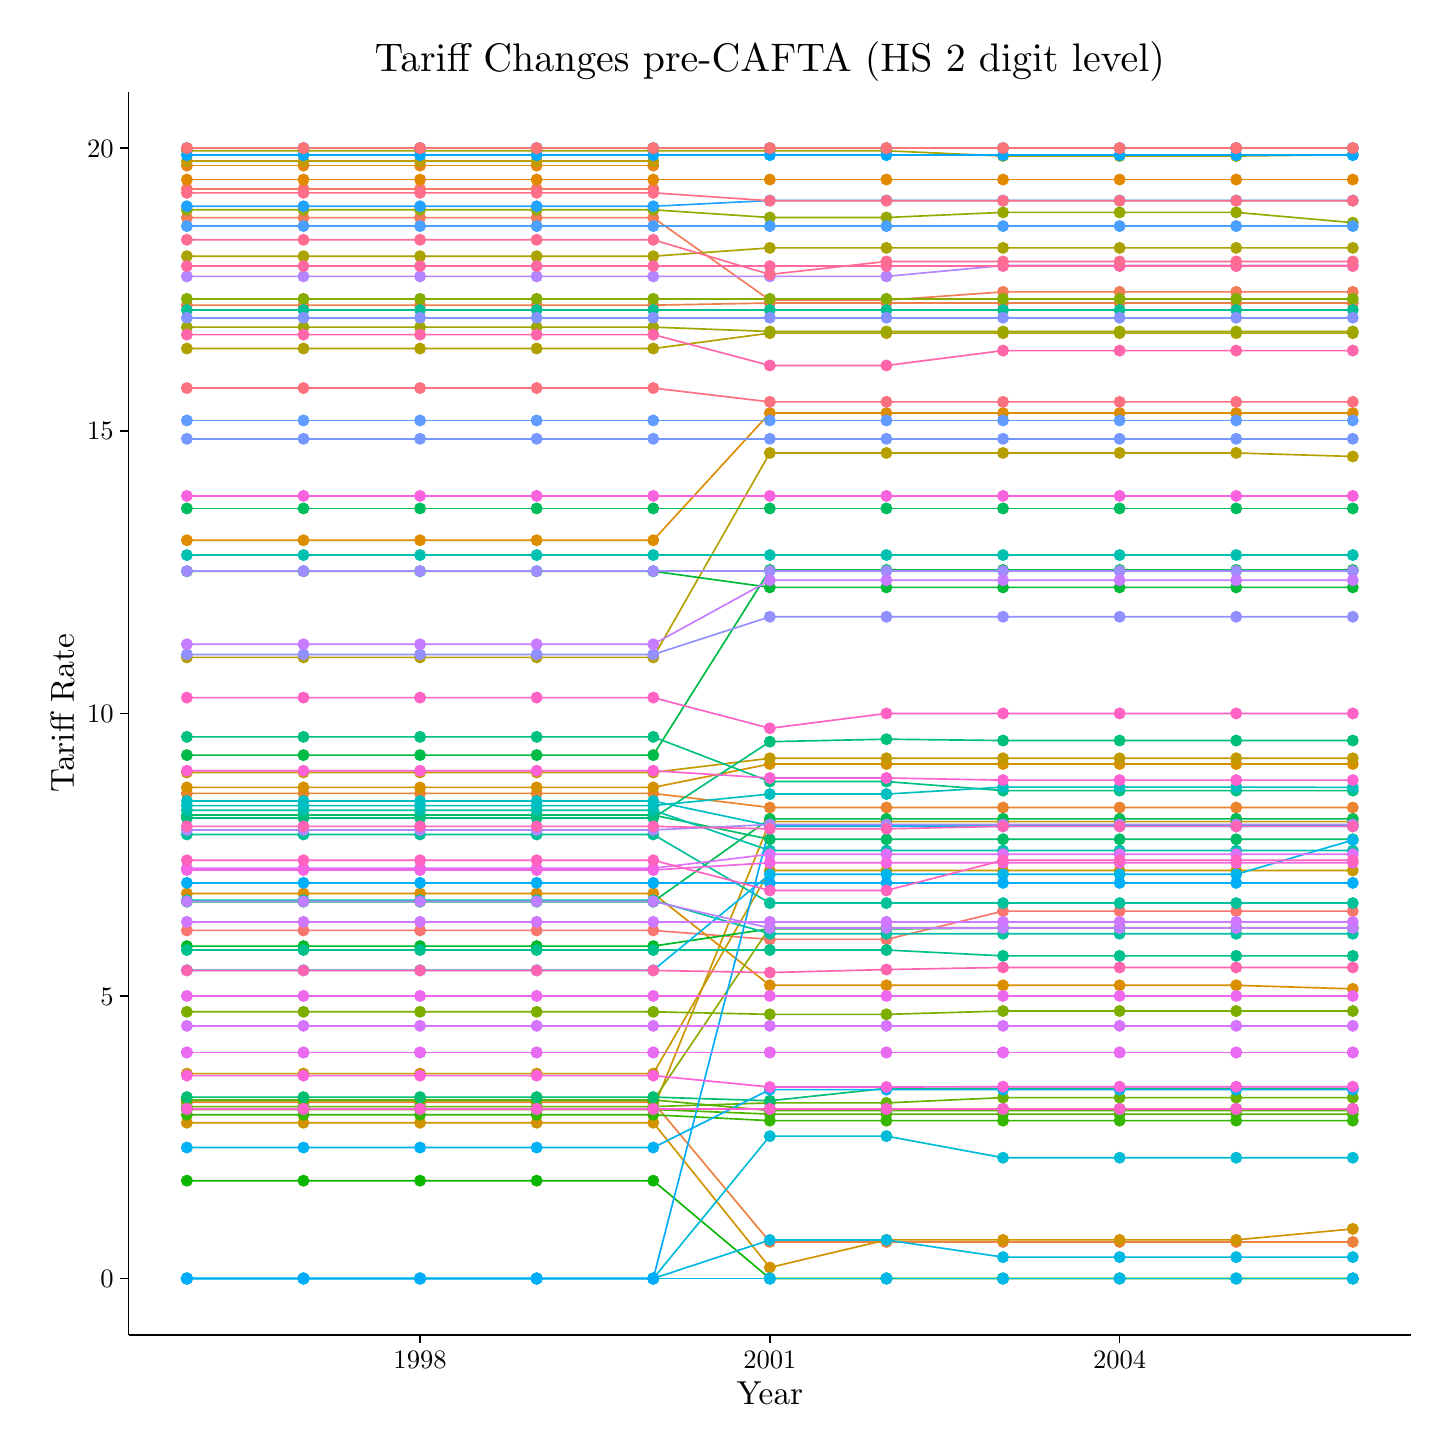
\begin{tikzpicture}[x=1pt,y=1pt]
\definecolor{fillColor}{RGB}{255,255,255}
\path[use as bounding box,fill=fillColor,fill opacity=0.00] (0,0) rectangle (505.89,505.89);
\begin{scope}
\path[clip] (  0.00,  0.00) rectangle (505.89,505.89);
\definecolor{drawColor}{RGB}{255,255,255}
\definecolor{fillColor}{RGB}{255,255,255}

\path[draw=drawColor,line width= 0.6pt,line join=round,line cap=round,fill=fillColor] (  0.00,  0.00) rectangle (505.89,505.89);
\end{scope}
\begin{scope}
\path[clip] ( 36.46, 33.48) rectangle (499.89,482.77);
\definecolor{fillColor}{RGB}{255,255,255}

\path[fill=fillColor] ( 36.46, 33.48) rectangle (499.89,482.77);
\definecolor{drawColor}{RGB}{248,118,109}

\path[draw=drawColor,line width= 0.6pt,line join=round] ( 57.53,179.68) --
	( 99.66,179.68) --
	(141.79,179.68) --
	(183.92,179.68) --
	(226.05,179.68) --
	(268.18,176.43) --
	(310.31,176.43) --
	(352.44,186.65) --
	(394.57,186.65) --
	(436.70,186.65) --
	(478.83,186.65);
\definecolor{drawColor}{RGB}{245,121,99}

\path[draw=drawColor,line width= 0.6pt,line join=round] ( 57.53,447.63) --
	( 99.66,447.63) --
	(141.79,447.63) --
	(183.92,447.63) --
	(226.05,447.63);
\definecolor{drawColor}{RGB}{243,124,88}

\path[draw=drawColor,line width= 0.6pt,line join=round] ( 57.53,437.23) --
	( 99.66,437.23) --
	(141.79,437.23) --
	(183.92,437.23) --
	(226.05,437.23) --
	(268.18,407.42) --
	(310.31,407.42) --
	(352.44,410.41) --
	(394.57,410.41) --
	(436.70,410.41) --
	(478.83,410.41);
\definecolor{drawColor}{RGB}{240,126,76}

\path[draw=drawColor,line width= 0.6pt,line join=round] ( 57.53,405.62) --
	( 99.66,405.62) --
	(141.79,405.62) --
	(183.92,405.62) --
	(226.05,405.62) --
	(268.18,406.38) --
	(310.31,406.38) --
	(352.44,406.38) --
	(394.57,406.38) --
	(436.70,406.38) --
	(478.83,406.38);
\definecolor{drawColor}{RGB}{237,129,62}

\path[draw=drawColor,line width= 0.6pt,line join=round] ( 57.53,117.57) --
	( 99.66,117.57) --
	(141.79,117.57) --
	(183.92,117.57) --
	(226.05,117.57) --
	(268.18, 67.11) --
	(310.31, 67.11) --
	(352.44, 67.11) --
	(394.57, 67.11) --
	(436.70, 67.11) --
	(478.83, 67.11);
\definecolor{drawColor}{RGB}{234,132,45}

\path[draw=drawColor,line width= 0.6pt,line join=round] ( 57.53,229.19) --
	( 99.66,229.19) --
	(141.79,229.19) --
	(183.92,229.19) --
	(226.05,229.19) --
	(268.18,224.09) --
	(310.31,224.09) --
	(352.44,224.09) --
	(394.57,224.09) --
	(436.70,224.09) --
	(478.83,224.09);
\definecolor{drawColor}{RGB}{230,134,19}

\path[draw=drawColor,line width= 0.6pt,line join=round] ( 57.53,456.04) --
	( 99.66,456.04) --
	(141.79,456.04) --
	(183.92,456.04) --
	(226.05,456.04);
\definecolor{drawColor}{RGB}{226,137,0}

\path[draw=drawColor,line width= 0.6pt,line join=round] ( 57.53,451.00) --
	( 99.66,451.00) --
	(141.79,451.00) --
	(183.92,451.00) --
	(226.05,451.00) --
	(268.18,451.00) --
	(310.31,451.00) --
	(352.44,451.00) --
	(394.57,451.00) --
	(436.70,451.00) --
	(478.83,451.00);
\definecolor{drawColor}{RGB}{222,140,0}

\path[draw=drawColor,line width= 0.6pt,line join=round] ( 57.53,320.67) --
	( 99.66,320.67) --
	(141.79,320.67) --
	(183.92,320.67) --
	(226.05,320.67) --
	(268.18,366.62) --
	(310.31,366.62) --
	(352.44,366.62) --
	(394.57,366.62) --
	(436.70,366.62) --
	(478.83,366.62);
\definecolor{drawColor}{RGB}{218,142,0}

\path[draw=drawColor,line width= 0.6pt,line join=round] ( 57.53,193.03) --
	( 99.66,193.03) --
	(141.79,193.03) --
	(183.92,193.03) --
	(226.05,193.03) --
	(268.18,159.84) --
	(310.31,159.84) --
	(352.44,159.84) --
	(394.57,159.84) --
	(436.70,159.84) --
	(478.83,158.56);
\definecolor{drawColor}{RGB}{214,145,0}

\path[draw=drawColor,line width= 0.6pt,line join=round] ( 57.53,231.36) --
	( 99.66,231.36) --
	(141.79,231.36) --
	(183.92,231.36) --
	(226.05,231.36) --
	(268.18,239.81) --
	(310.31,239.81) --
	(352.44,239.81) --
	(394.57,239.81) --
	(436.70,239.81) --
	(478.83,239.81);
\definecolor{drawColor}{RGB}{209,147,0}

\path[draw=drawColor,line width= 0.6pt,line join=round] ( 57.53,110.19) --
	( 99.66,110.19) --
	(141.79,110.19) --
	(183.92,110.19) --
	(226.05,110.19) --
	(268.18, 57.88) --
	(310.31, 67.85) --
	(352.44, 67.85) --
	(394.57, 67.85) --
	(436.70, 67.85) --
	(478.83, 71.83);
\definecolor{drawColor}{RGB}{205,150,0}

\path[draw=drawColor,line width= 0.6pt,line join=round] ( 57.53,115.17) --
	( 99.66,115.17) --
	(141.79,115.17) --
	(183.92,115.17) --
	(226.05,115.17) --
	(268.18,218.98) --
	(310.31,218.98) --
	(352.44,218.98) --
	(394.57,218.98) --
	(436.70,218.98) --
	(478.83,218.98);
\definecolor{drawColor}{RGB}{200,152,0}

\path[draw=drawColor,line width= 0.6pt,line join=round] ( 57.53,127.93) --
	( 99.66,127.93) --
	(141.79,127.93) --
	(183.92,127.93) --
	(226.05,127.93) --
	(268.18,201.32) --
	(310.31,201.32) --
	(352.44,201.32) --
	(394.57,201.32) --
	(436.70,201.32) --
	(478.83,201.32);
\definecolor{drawColor}{RGB}{194,154,0}

\path[draw=drawColor,line width= 0.6pt,line join=round] ( 57.53,236.77) --
	( 99.66,236.77) --
	(141.79,236.77) --
	(183.92,236.77) --
	(226.05,236.77) --
	(268.18,241.88) --
	(310.31,241.88) --
	(352.44,241.88) --
	(394.57,241.88) --
	(436.70,241.88) --
	(478.83,241.88);
\definecolor{drawColor}{RGB}{189,157,0}

\path[draw=drawColor,line width= 0.6pt,line join=round] ( 57.53,457.64) --
	( 99.66,457.64) --
	(141.79,457.64) --
	(183.92,457.64) --
	(226.05,457.64);
\definecolor{drawColor}{RGB}{183,159,0}

\path[draw=drawColor,line width= 0.6pt,line join=round] ( 57.53,278.33) --
	( 99.66,278.33) --
	(141.79,278.33) --
	(183.92,278.33) --
	(226.05,278.33) --
	(268.18,352.21) --
	(310.31,352.21) --
	(352.44,352.21) --
	(394.57,352.21) --
	(436.70,352.21) --
	(478.83,350.94);
\definecolor{drawColor}{RGB}{177,161,0}

\path[draw=drawColor,line width= 0.6pt,line join=round] ( 57.53,389.94) --
	( 99.66,389.94) --
	(141.79,389.94) --
	(183.92,389.94) --
	(226.05,389.94) --
	(268.18,395.51) --
	(310.31,395.51) --
	(352.44,395.51) --
	(394.57,395.51) --
	(436.70,395.51) --
	(478.83,395.51);
\definecolor{drawColor}{RGB}{171,163,0}

\path[draw=drawColor,line width= 0.6pt,line join=round] ( 57.53,423.31) --
	( 99.66,423.31) --
	(141.79,423.31) --
	(183.92,423.31) --
	(226.05,423.31) --
	(268.18,426.31) --
	(310.31,426.31) --
	(352.44,426.31) --
	(394.57,426.31) --
	(436.70,426.31) --
	(478.83,426.31);
\definecolor{drawColor}{RGB}{164,165,0}

\path[draw=drawColor,line width= 0.6pt,line join=round] ( 57.53,461.40) --
	( 99.66,461.40) --
	(141.79,461.40) --
	(183.92,461.40) --
	(226.05,461.40) --
	(268.18,461.40) --
	(310.31,461.40) --
	(352.44,459.50) --
	(394.57,459.50) --
	(436.70,459.50) --
	(478.83,459.98);
\definecolor{drawColor}{RGB}{157,167,0}

\path[draw=drawColor,line width= 0.6pt,line join=round] ( 57.53,397.68) --
	( 99.66,397.68) --
	(141.79,397.68) --
	(183.92,397.68) --
	(226.05,397.68) --
	(268.18,396.10) --
	(310.31,396.10) --
	(352.44,396.10) --
	(394.57,396.10) --
	(436.70,396.10) --
	(478.83,396.10);
\definecolor{drawColor}{RGB}{150,169,0}

\path[draw=drawColor,line width= 0.6pt,line join=round] ( 57.53,440.07) --
	( 99.66,440.07) --
	(141.79,440.07) --
	(183.92,440.07) --
	(226.05,440.07) --
	(268.18,437.29) --
	(310.31,437.29) --
	(352.44,439.14) --
	(394.57,439.14) --
	(436.70,439.14) --
	(478.83,435.43);
\definecolor{drawColor}{RGB}{142,171,0}

\path[draw=drawColor,line width= 0.6pt,line join=round] ( 57.53,118.14) --
	( 99.66,118.14) --
	(141.79,118.14) --
	(183.92,118.14) --
	(226.05,118.14) --
	(268.18,180.69) --
	(310.31,180.69) --
	(352.44,180.69) --
	(394.57,180.69) --
	(436.70,180.69) --
	(478.83,180.69);
\definecolor{drawColor}{RGB}{133,173,0}

\path[draw=drawColor,line width= 0.6pt,line join=round] ( 57.53,407.89) --
	( 99.66,407.89) --
	(141.79,407.89) --
	(183.92,407.89) --
	(226.05,407.89) --
	(268.18,407.89) --
	(310.31,407.89) --
	(352.44,407.89) --
	(394.57,407.89) --
	(436.70,407.89) --
	(478.83,407.89);
\definecolor{drawColor}{RGB}{124,174,0}

\path[draw=drawColor,line width= 0.6pt,line join=round] ( 57.53,150.27) --
	( 99.66,150.27) --
	(141.79,150.27) --
	(183.92,150.27) --
	(226.05,150.27) --
	(268.18,149.35) --
	(310.31,149.35) --
	(352.44,150.55) --
	(394.57,150.55) --
	(436.70,150.55) --
	(478.83,150.55);
\definecolor{drawColor}{RGB}{113,176,0}

\path[draw=drawColor,line width= 0.6pt,line join=round] ( 57.53,115.17) --
	( 99.66,115.17) --
	(141.79,115.17) --
	(183.92,115.17) --
	(226.05,115.17) --
	(268.18,115.17) --
	(310.31,115.17) --
	(352.44,115.17) --
	(394.57,115.17) --
	(436.70,115.17) --
	(478.83,115.17);
\definecolor{drawColor}{RGB}{102,178,0}

\path[draw=drawColor,line width= 0.6pt,line join=round] ( 57.53,116.02) --
	( 99.66,116.02) --
	(141.79,116.02) --
	(183.92,116.02) --
	(226.05,116.02) --
	(268.18,117.35) --
	(310.31,117.35) --
	(352.44,119.26) --
	(394.57,119.26) --
	(436.70,119.26) --
	(478.83,119.26);
\definecolor{drawColor}{RGB}{89,179,0}

\path[draw=drawColor,line width= 0.6pt,line join=round] ( 57.53,118.44) --
	( 99.66,118.44) --
	(141.79,118.44) --
	(183.92,118.44) --
	(226.05,118.44) --
	(268.18,114.57) --
	(310.31,114.57) --
	(352.44,114.57) --
	(394.57,114.57) --
	(436.70,114.57) --
	(478.83,114.57);
\definecolor{drawColor}{RGB}{73,181,0}

\path[draw=drawColor,line width= 0.6pt,line join=round] ( 57.53,114.97) --
	( 99.66,114.97) --
	(141.79,114.97) --
	(183.92,114.97) --
	(226.05,114.97) --
	(268.18,113.31) --
	(310.31,113.31) --
	(352.44,113.31) --
	(394.57,113.31) --
	(436.70,113.31) --
	(478.83,113.31);
\definecolor{drawColor}{RGB}{53,182,0}

\path[draw=drawColor,line width= 0.6pt,line join=round] ( 57.53,113.05) --
	( 99.66,113.05) --
	(141.79,113.05) --
	(183.92,113.05) --
	(226.05,113.05) --
	(268.18,110.94) --
	(310.31,110.94) --
	(352.44,110.94) --
	(394.57,110.94) --
	(436.70,110.94) --
	(478.83,110.94);
\definecolor{drawColor}{RGB}{12,183,2}

\path[draw=drawColor,line width= 0.6pt,line join=round] ( 57.53, 89.25) --
	( 99.66, 89.25) --
	(141.79, 89.25) --
	(183.92, 89.25) --
	(226.05, 89.25) --
	(268.18, 53.90) --
	(310.31, 53.90) --
	(352.44, 53.90) --
	(394.57, 53.90) --
	(436.70, 53.90) --
	(478.83, 53.90);
\definecolor{drawColor}{RGB}{0,185,38}

\path[draw=drawColor,line width= 0.6pt,line join=round] ( 57.53,174.01) --
	( 99.66,174.01) --
	(141.79,174.01) --
	(183.92,174.01) --
	(226.05,174.01) --
	(268.18,180.25) --
	(310.31,180.25) --
	(352.44,180.52) --
	(394.57,180.52) --
	(436.70,180.52) --
	(478.83,180.52);
\definecolor{drawColor}{RGB}{0,186,56}

\path[draw=drawColor,line width= 0.6pt,line join=round] ( 57.53,309.47) --
	( 99.66,309.47) --
	(141.79,309.47) --
	(183.92,309.47) --
	(226.05,309.47) --
	(268.18,303.64) --
	(310.31,303.64) --
	(352.44,303.64) --
	(394.57,303.64) --
	(436.70,303.64) --
	(478.83,303.64);
\definecolor{drawColor}{RGB}{0,187,70}

\path[draw=drawColor,line width= 0.6pt,line join=round] ( 57.53,243.03) --
	( 99.66,243.03) --
	(141.79,243.03) --
	(183.92,243.03) --
	(226.05,243.03) --
	(268.18,309.92) --
	(310.31,309.92) --
	(352.44,309.92) --
	(394.57,309.92) --
	(436.70,309.92) --
	(478.83,309.92);
\definecolor{drawColor}{RGB}{0,188,82}

\path[draw=drawColor,line width= 0.6pt,line join=round] ( 57.53,190.05) --
	( 99.66,190.05) --
	(141.79,190.05) --
	(183.92,190.05) --
	(226.05,190.05) --
	(268.18,220.00) --
	(310.31,220.00) --
	(352.44,220.00) --
	(394.57,220.00) --
	(436.70,220.00) --
	(478.83,220.00);
\definecolor{drawColor}{RGB}{0,189,93}

\path[draw=drawColor,line width= 0.6pt,line join=round] ( 57.53,332.16) --
	( 99.66,332.16) --
	(141.79,332.16) --
	(183.92,332.16) --
	(226.05,332.16) --
	(268.18,332.16) --
	(310.31,332.16) --
	(352.44,332.16) --
	(394.57,332.16) --
	(436.70,332.16) --
	(478.83,332.16);
\definecolor{drawColor}{RGB}{0,190,103}

\path[draw=drawColor,line width= 0.6pt,line join=round] ( 57.53,221.36) --
	( 99.66,221.36) --
	(141.79,221.36) --
	(183.92,221.36) --
	(226.05,221.36) --
	(268.18,212.61) --
	(310.31,212.61) --
	(352.44,212.61) --
	(394.57,212.61) --
	(436.70,212.61) --
	(478.83,212.61);
\definecolor{drawColor}{RGB}{0,190,113}

\path[draw=drawColor,line width= 0.6pt,line join=round] ( 57.53,119.45) --
	( 99.66,119.45) --
	(141.79,119.45) --
	(183.92,119.45) --
	(226.05,119.45) --
	(268.18,118.13) --
	(310.31,122.61) --
	(352.44,122.61) --
	(394.57,122.61) --
	(436.70,122.61) --
	(478.83,122.61);
\definecolor{drawColor}{RGB}{0,191,122}

\path[draw=drawColor,line width= 0.6pt,line join=round] ( 57.53,220.31) --
	( 99.66,220.31) --
	(141.79,220.31) --
	(183.92,220.31) --
	(226.05,220.31) --
	(268.18,247.88) --
	(310.31,248.78) --
	(352.44,248.29) --
	(394.57,248.29) --
	(436.70,248.29) --
	(478.83,248.29);
\definecolor{drawColor}{RGB}{0,192,130}

\path[draw=drawColor,line width= 0.6pt,line join=round] ( 57.53,249.62) --
	( 99.66,249.62) --
	(141.79,249.62) --
	(183.92,249.62) --
	(226.05,249.62) --
	(268.18,233.47) --
	(310.31,233.47) --
	(352.44,230.20) --
	(394.57,230.20) --
	(436.70,230.20) --
	(478.83,230.20);
\definecolor{drawColor}{RGB}{0,192,139}

\path[draw=drawColor,line width= 0.6pt,line join=round] ( 57.53,172.60) --
	( 99.66,172.60) --
	(141.79,172.60) --
	(183.92,172.60) --
	(226.05,172.60) --
	(268.18,172.60) --
	(310.31,172.60) --
	(352.44,170.48) --
	(394.57,170.48) --
	(436.70,170.48) --
	(478.83,170.48);
\definecolor{drawColor}{RGB}{0,192,147}

\path[draw=drawColor,line width= 0.6pt,line join=round] ( 57.53,403.87) --
	( 99.66,403.87) --
	(141.79,403.87) --
	(183.92,403.87) --
	(226.05,403.87) --
	(268.18,403.87) --
	(310.31,403.87) --
	(352.44,403.87) --
	(394.57,403.87) --
	(436.70,403.87) --
	(478.83,403.87);
\definecolor{drawColor}{RGB}{0,193,154}

\path[draw=drawColor,line width= 0.6pt,line join=round] ( 57.53,214.36) --
	( 99.66,214.36) --
	(141.79,214.36) --
	(183.92,214.36) --
	(226.05,214.36) --
	(268.18,189.56) --
	(310.31,189.56) --
	(352.44,189.56) --
	(394.57,189.56) --
	(436.70,189.56) --
	(478.83,189.56);
\definecolor{drawColor}{RGB}{0,193,162}

\path[draw=drawColor,line width= 0.6pt,line join=round] ( 57.53,190.59) --
	( 99.66,190.59) --
	(141.79,190.59) --
	(183.92,190.59) --
	(226.05,190.59) --
	(268.18,178.47) --
	(310.31,178.47) --
	(352.44,178.47) --
	(394.57,178.47) --
	(436.70,178.47) --
	(478.83,178.47);
\definecolor{drawColor}{RGB}{0,193,169}

\path[draw=drawColor,line width= 0.6pt,line join=round] ( 57.53,223.11) --
	( 99.66,223.11) --
	(141.79,223.11) --
	(183.92,223.11) --
	(226.05,223.11) --
	(268.18,208.53) --
	(310.31,208.53) --
	(352.44,208.53) --
	(394.57,208.53) --
	(436.70,208.53) --
	(478.83,208.53);
\definecolor{drawColor}{RGB}{0,192,176}

\path[draw=drawColor,line width= 0.6pt,line join=round] ( 57.53,315.31) --
	( 99.66,315.31) --
	(141.79,315.31) --
	(183.92,315.31) --
	(226.05,315.31) --
	(268.18,315.31) --
	(310.31,315.31) --
	(352.44,315.31) --
	(394.57,315.31) --
	(436.70,315.31) --
	(478.83,315.31);
\definecolor{drawColor}{RGB}{0,192,183}

\path[draw=drawColor,line width= 0.6pt,line join=round] ( 57.53,115.17) --
	( 99.66,115.17) --
	(141.79,115.17) --
	(183.92,115.17) --
	(226.05,115.17) --
	(268.18,115.17) --
	(310.31,115.17) --
	(352.44,115.17) --
	(394.57,115.17) --
	(436.70,115.17) --
	(478.83,115.17);
\definecolor{drawColor}{RGB}{0,192,190}

\path[draw=drawColor,line width= 0.6pt,line join=round] ( 57.53,224.79) --
	( 99.66,224.79) --
	(141.79,224.79) --
	(183.92,224.79) --
	(226.05,224.79) --
	(268.18,228.95) --
	(310.31,228.95) --
	(352.44,231.46) --
	(394.57,231.46) --
	(436.70,231.46) --
	(478.83,231.35);
\definecolor{drawColor}{RGB}{0,191,196}

\path[draw=drawColor,line width= 0.6pt,line join=round] ( 57.53,226.42) --
	( 99.66,226.42) --
	(141.79,226.42) --
	(183.92,226.42) --
	(226.05,226.42) --
	(268.18,217.55) --
	(310.31,217.55) --
	(352.44,217.55) --
	(394.57,217.55) --
	(436.70,217.55) --
	(478.83,217.55);
\definecolor{drawColor}{RGB}{0,190,203}

\path[draw=drawColor,line width= 0.6pt,line join=round] ( 57.53, 53.90) --
	( 99.66, 53.90) --
	(141.79, 53.90) --
	(183.92, 53.90) --
	(226.05, 53.90) --
	(268.18, 53.90) --
	(310.31, 53.90) --
	(352.44, 53.90) --
	(394.57, 53.90) --
	(436.70, 53.90) --
	(478.83, 53.90);
\definecolor{drawColor}{RGB}{0,189,209}

\path[draw=drawColor,line width= 0.6pt,line join=round] ( 57.53, 53.90) --
	( 99.66, 53.90) --
	(141.79, 53.90) --
	(183.92, 53.90) --
	(226.05, 53.90) --
	(268.18, 53.90) --
	(310.31, 53.90) --
	(352.44, 53.90) --
	(394.57, 53.90) --
	(436.70, 53.90) --
	(478.83, 53.90);
\definecolor{drawColor}{RGB}{0,188,215}

\path[draw=drawColor,line width= 0.6pt,line join=round] ( 57.53, 53.90) --
	( 99.66, 53.90) --
	(141.79, 53.90) --
	(183.92, 53.90) --
	(226.05, 53.90) --
	(268.18,105.35) --
	(310.31,105.35) --
	(352.44, 97.55) --
	(394.57, 97.55) --
	(436.70, 97.55) --
	(478.83, 97.55);
\definecolor{drawColor}{RGB}{0,187,220}

\path[draw=drawColor,line width= 0.6pt,line join=round] ( 57.53, 53.90) --
	( 99.66, 53.90) --
	(141.79, 53.90) --
	(183.92, 53.90) --
	(226.05, 53.90) --
	(268.18, 53.90) --
	(310.31, 53.90) --
	(352.44, 53.90) --
	(394.57, 53.90) --
	(436.70, 53.90) --
	(478.83, 53.90);
\definecolor{drawColor}{RGB}{0,185,226}

\path[draw=drawColor,line width= 0.6pt,line join=round] ( 57.53, 53.90) --
	( 99.66, 53.90) --
	(141.79, 53.90) --
	(183.92, 53.90) --
	(226.05, 53.90) --
	(268.18, 67.82) --
	(310.31, 67.82) --
	(352.44, 61.63) --
	(394.57, 61.63) --
	(436.70, 61.63) --
	(478.83, 61.63);
\definecolor{drawColor}{RGB}{0,184,231}

\path[draw=drawColor,line width= 0.6pt,line join=round] ( 57.53, 53.90) --
	( 99.66, 53.90) --
	(141.79, 53.90) --
	(183.92, 53.90) --
	(226.05, 53.90) --
	(268.18, 53.90) --
	(310.31, 53.90) --
	(352.44, 53.90) --
	(394.57, 53.90) --
	(436.70, 53.90) --
	(478.83, 53.90);
\definecolor{drawColor}{RGB}{0,182,235}

\path[draw=drawColor,line width= 0.6pt,line join=round] ( 57.53,165.29) --
	( 99.66,165.29) --
	(141.79,165.29) --
	(183.92,165.29) --
	(226.05,165.29) --
	(268.18,199.95) --
	(310.31,199.95) --
	(352.44,199.95) --
	(394.57,199.95) --
	(436.70,199.95) --
	(478.83,212.33);
\definecolor{drawColor}{RGB}{0,180,240}

\path[draw=drawColor,line width= 0.6pt,line join=round] ( 57.53,462.35) --
	( 99.66,462.35) --
	(141.79,462.35) --
	(183.92,462.35) --
	(226.05,462.35) --
	(268.18,462.35) --
	(310.31,462.35) --
	(352.44,462.35) --
	(394.57,462.35) --
	(436.70,462.35) --
	(478.83,462.35);
\definecolor{drawColor}{RGB}{0,177,244}

\path[draw=drawColor,line width= 0.6pt,line join=round] ( 57.53,101.22) --
	( 99.66,101.22) --
	(141.79,101.22) --
	(183.92,101.22) --
	(226.05,101.22) --
	(268.18,122.14) --
	(310.31,122.14) --
	(352.44,122.14) --
	(394.57,122.14) --
	(436.70,122.14) --
	(478.83,122.14);
\definecolor{drawColor}{RGB}{0,175,248}

\path[draw=drawColor,line width= 0.6pt,line join=round] ( 57.53,196.86) --
	( 99.66,196.86) --
	(141.79,196.86) --
	(183.92,196.86) --
	(226.05,196.86) --
	(268.18,196.86) --
	(310.31,196.86) --
	(352.44,196.86) --
	(394.57,196.86) --
	(436.70,196.86) --
	(478.83,196.86);
\definecolor{drawColor}{RGB}{0,172,251}

\path[draw=drawColor,line width= 0.6pt,line join=round] ( 57.53, 53.90) --
	( 99.66, 53.90) --
	(141.79, 53.90) --
	(183.92, 53.90) --
	(226.05, 53.90) --
	(268.18,217.28) --
	(310.31,217.28) --
	(352.44,217.28) --
	(394.57,217.28) --
	(436.70,217.28) --
	(478.83,217.28);
\definecolor{drawColor}{RGB}{0,169,255}

\path[draw=drawColor,line width= 0.6pt,line join=round] ( 57.53,459.81) --
	( 99.66,459.81) --
	(141.79,459.81) --
	(183.92,459.81) --
	(226.05,459.81) --
	(268.18,459.81) --
	(310.31,459.81) --
	(352.44,459.81) --
	(394.57,459.81) --
	(436.70,459.81) --
	(478.83,459.81);
\definecolor{drawColor}{RGB}{0,166,255}

\path[draw=drawColor,line width= 0.6pt,line join=round] ( 57.53,462.35) --
	( 99.66,462.35) --
	(141.79,462.35) --
	(183.92,462.35) --
	(226.05,462.35) --
	(268.18,462.35) --
	(310.31,462.35) --
	(352.44,462.35) --
	(394.57,462.35) --
	(436.70,462.35) --
	(478.83,462.35);
\definecolor{drawColor}{RGB}{34,163,255}

\path[draw=drawColor,line width= 0.6pt,line join=round] ( 57.53,441.35) --
	( 99.66,441.35) --
	(141.79,441.35) --
	(183.92,441.35) --
	(226.05,441.35) --
	(268.18,443.43) --
	(310.31,443.43) --
	(352.44,443.43) --
	(394.57,443.43) --
	(436.70,443.43) --
	(478.83,443.43);
\definecolor{drawColor}{RGB}{73,160,255}

\path[draw=drawColor,line width= 0.6pt,line join=round] ( 57.53,434.18) --
	( 99.66,434.18) --
	(141.79,434.18) --
	(183.92,434.18) --
	(226.05,434.18) --
	(268.18,434.18) --
	(310.31,434.18) --
	(352.44,434.18) --
	(394.57,434.18) --
	(436.70,434.18) --
	(478.83,434.18);
\definecolor{drawColor}{RGB}{97,156,255}

\path[draw=drawColor,line width= 0.6pt,line join=round] ( 57.53,363.95) --
	( 99.66,363.95) --
	(141.79,363.95) --
	(183.92,363.95) --
	(226.05,363.95) --
	(268.18,363.95) --
	(310.31,363.95) --
	(352.44,363.95) --
	(394.57,363.95) --
	(436.70,363.95) --
	(478.83,363.95);
\definecolor{drawColor}{RGB}{116,152,255}

\path[draw=drawColor,line width= 0.6pt,line join=round] ( 57.53,357.32) --
	( 99.66,357.32) --
	(141.79,357.32) --
	(183.92,357.32) --
	(226.05,357.32) --
	(268.18,357.32) --
	(310.31,357.32) --
	(352.44,357.32) --
	(394.57,357.32) --
	(436.70,357.32) --
	(478.83,357.32);
\definecolor{drawColor}{RGB}{132,148,255}

\path[draw=drawColor,line width= 0.6pt,line join=round] ( 57.53,401.08) --
	( 99.66,401.08) --
	(141.79,401.08) --
	(183.92,401.08) --
	(226.05,401.08) --
	(268.18,401.08) --
	(310.31,401.08) --
	(352.44,401.08) --
	(394.57,401.08) --
	(436.70,401.08) --
	(478.83,401.08);
\definecolor{drawColor}{RGB}{146,144,255}

\path[draw=drawColor,line width= 0.6pt,line join=round] ( 57.53,279.40) --
	( 99.66,279.40) --
	(141.79,279.40) --
	(183.92,279.40) --
	(226.05,279.40) --
	(268.18,293.01) --
	(310.31,293.01) --
	(352.44,293.01) --
	(394.57,293.01) --
	(436.70,293.01) --
	(478.83,293.01);
\definecolor{drawColor}{RGB}{159,140,255}

\path[draw=drawColor,line width= 0.6pt,line join=round] ( 57.53,309.53) --
	( 99.66,309.53) --
	(141.79,309.53) --
	(183.92,309.53) --
	(226.05,309.53) --
	(268.18,309.53) --
	(310.31,309.53) --
	(352.44,309.53) --
	(394.57,309.53) --
	(436.70,309.53) --
	(478.83,309.53);
\definecolor{drawColor}{RGB}{170,136,255}

\path[draw=drawColor,line width= 0.6pt,line join=round] ( 57.53,215.98) --
	( 99.66,215.98) --
	(141.79,215.98) --
	(183.92,215.98) --
	(226.05,215.98) --
	(268.18,217.93) --
	(310.31,217.93) --
	(352.44,217.93) --
	(394.57,217.93) --
	(436.70,217.93) --
	(478.83,217.93);
\definecolor{drawColor}{RGB}{181,132,255}

\path[draw=drawColor,line width= 0.6pt,line join=round] ( 57.53,416.01) --
	( 99.66,416.01) --
	(141.79,416.01) --
	(183.92,416.01) --
	(226.05,416.01) --
	(268.18,416.01) --
	(310.31,416.01) --
	(352.44,419.93) --
	(394.57,419.93) --
	(436.70,419.93) --
	(478.83,419.93);
\definecolor{drawColor}{RGB}{190,128,255}

\path[draw=drawColor,line width= 0.6pt,line join=round] ( 57.53,190.17) --
	( 99.66,190.17) --
	(141.79,190.17) --
	(183.92,190.17) --
	(226.05,190.17) --
	(268.18,180.55) --
	(310.31,180.55) --
	(352.44,180.55) --
	(394.57,180.55) --
	(436.70,180.55) --
	(478.83,180.55);
\definecolor{drawColor}{RGB}{199,124,255}

\path[draw=drawColor,line width= 0.6pt,line join=round] ( 57.53,283.08) --
	( 99.66,283.08) --
	(141.79,283.08) --
	(183.92,283.08) --
	(226.05,283.08) --
	(268.18,306.20) --
	(310.31,306.20) --
	(352.44,306.20) --
	(394.57,306.20) --
	(436.70,306.20) --
	(478.83,306.20);
\definecolor{drawColor}{RGB}{207,120,255}

\path[draw=drawColor,line width= 0.6pt,line join=round] ( 57.53,182.77) --
	( 99.66,182.77) --
	(141.79,182.77) --
	(183.92,182.77) --
	(226.05,182.77) --
	(268.18,182.77) --
	(310.31,182.77) --
	(352.44,182.77) --
	(394.57,182.77) --
	(436.70,182.77) --
	(478.83,182.77);
\definecolor{drawColor}{RGB}{214,116,253}

\path[draw=drawColor,line width= 0.6pt,line join=round] ( 57.53,145.20) --
	( 99.66,145.20) --
	(141.79,145.20) --
	(183.92,145.20) --
	(226.05,145.20) --
	(268.18,145.20) --
	(310.31,145.20) --
	(352.44,145.20) --
	(394.57,145.20) --
	(436.70,145.20) --
	(478.83,145.20);
\definecolor{drawColor}{RGB}{221,113,250}

\path[draw=drawColor,line width= 0.6pt,line join=round] ( 57.53,202.15) --
	( 99.66,202.15) --
	(141.79,202.15) --
	(183.92,202.15) --
	(226.05,202.15) --
	(268.18,207.21) --
	(310.31,207.21) --
	(352.44,207.21) --
	(394.57,207.21) --
	(436.70,207.21) --
	(478.83,207.21);
\definecolor{drawColor}{RGB}{227,110,246}

\path[draw=drawColor,line width= 0.6pt,line join=round] ( 57.53,135.59) --
	( 99.66,135.59) --
	(141.79,135.59) --
	(183.92,135.59) --
	(226.05,135.59) --
	(268.18,135.59) --
	(310.31,135.59) --
	(352.44,135.59) --
	(394.57,135.59) --
	(436.70,135.59) --
	(478.83,135.59);
\definecolor{drawColor}{RGB}{232,107,242}

\path[draw=drawColor,line width= 0.6pt,line join=round] ( 57.53,135.59) --
	( 99.66,135.59) --
	(141.79,135.59) --
	(183.92,135.59) --
	(226.05,135.59) --
	(268.18,135.59) --
	(310.31,135.59) --
	(352.44,135.59) --
	(394.57,135.59) --
	(436.70,135.59) --
	(478.83,135.59);
\definecolor{drawColor}{RGB}{237,104,237}

\path[draw=drawColor,line width= 0.6pt,line join=round] ( 57.53,156.01) --
	( 99.66,156.01) --
	(141.79,156.01) --
	(183.92,156.01) --
	(226.05,156.01) --
	(268.18,156.01) --
	(310.31,156.01) --
	(352.44,156.01) --
	(394.57,156.01) --
	(436.70,156.01) --
	(478.83,156.01);
\definecolor{drawColor}{RGB}{241,102,233}

\path[draw=drawColor,line width= 0.6pt,line join=round] ( 57.53,115.17) --
	( 99.66,115.17) --
	(141.79,115.17) --
	(183.92,115.17) --
	(226.05,115.17) --
	(268.18,115.17) --
	(310.31,115.17) --
	(352.44,115.17) --
	(394.57,115.17) --
	(436.70,115.17) --
	(478.83,115.17);
\definecolor{drawColor}{RGB}{245,100,227}

\path[draw=drawColor,line width= 0.6pt,line join=round] ( 57.53,201.50) --
	( 99.66,201.50) --
	(141.79,201.50) --
	(183.92,201.50) --
	(226.05,201.50) --
	(268.18,204.13) --
	(310.31,204.13) --
	(352.44,204.13) --
	(394.57,204.13) --
	(436.70,204.13) --
	(478.83,204.13);
\definecolor{drawColor}{RGB}{248,98,222}

\path[draw=drawColor,line width= 0.6pt,line join=round] ( 57.53,336.69) --
	( 99.66,336.69) --
	(141.79,336.69) --
	(183.92,336.69) --
	(226.05,336.69) --
	(268.18,336.69) --
	(310.31,336.69) --
	(352.44,336.69) --
	(394.57,336.69) --
	(436.70,336.69) --
	(478.83,336.69);
\definecolor{drawColor}{RGB}{251,97,216}

\path[draw=drawColor,line width= 0.6pt,line join=round] ( 57.53,127.22) --
	( 99.66,127.22) --
	(141.79,127.22) --
	(183.92,127.22) --
	(226.05,127.22) --
	(268.18,123.09) --
	(310.31,123.09) --
	(352.44,123.21) --
	(394.57,123.21) --
	(436.70,123.21) --
	(478.83,123.21);
\definecolor{drawColor}{RGB}{253,97,210}

\path[draw=drawColor,line width= 0.6pt,line join=round] ( 57.53,237.36) --
	( 99.66,237.36) --
	(141.79,237.36) --
	(183.92,237.36) --
	(226.05,237.36) --
	(268.18,234.77) --
	(310.31,234.77) --
	(352.44,233.98) --
	(394.57,233.98) --
	(436.70,233.98) --
	(478.83,233.98);
\definecolor{drawColor}{RGB}{255,97,204}

\path[draw=drawColor,line width= 0.6pt,line join=round] ( 57.53,115.17) --
	( 99.66,115.17) --
	(141.79,115.17) --
	(183.92,115.17) --
	(226.05,115.17) --
	(268.18,115.17) --
	(310.31,115.17) --
	(352.44,115.17) --
	(394.57,115.17) --
	(436.70,115.17) --
	(478.83,115.17);
\definecolor{drawColor}{RGB}{255,97,197}

\path[draw=drawColor,line width= 0.6pt,line join=round] ( 57.53,263.81) --
	( 99.66,263.81) --
	(141.79,263.81) --
	(183.92,263.81) --
	(226.05,263.81) --
	(268.18,252.72) --
	(310.31,258.09) --
	(352.44,258.09) --
	(394.57,258.09) --
	(436.70,258.09) --
	(478.83,258.09);
\definecolor{drawColor}{RGB}{255,98,191}

\path[draw=drawColor,line width= 0.6pt,line join=round] ( 57.53,205.03) --
	( 99.66,205.03) --
	(141.79,205.03) --
	(183.92,205.03) --
	(226.05,205.03) --
	(268.18,194.13) --
	(310.31,194.13) --
	(352.44,205.03) --
	(394.57,205.03) --
	(436.70,205.03) --
	(478.83,205.03);
\definecolor{drawColor}{RGB}{255,99,184}

\path[draw=drawColor,line width= 0.6pt,line join=round] ( 57.53,217.28) --
	( 99.66,217.28) --
	(141.79,217.28) --
	(183.92,217.28) --
	(226.05,217.28) --
	(268.18,216.38) --
	(310.31,216.38) --
	(352.44,217.28) --
	(394.57,217.28) --
	(436.70,217.28) --
	(478.83,217.28);
\definecolor{drawColor}{RGB}{255,100,176}

\path[draw=drawColor,line width= 0.6pt,line join=round] ( 57.53,165.22) --
	( 99.66,165.22) --
	(141.79,165.22) --
	(183.92,165.22) --
	(226.05,165.22) --
	(268.18,164.46) --
	(310.31,165.54) --
	(352.44,166.31) --
	(394.57,166.31) --
	(436.70,166.31) --
	(478.83,166.31);
\definecolor{drawColor}{RGB}{255,102,169}

\path[draw=drawColor,line width= 0.6pt,line join=round] ( 57.53,394.98) --
	( 99.66,394.98) --
	(141.79,394.98) --
	(183.92,394.98) --
	(226.05,394.98) --
	(268.18,383.81) --
	(310.31,383.81) --
	(352.44,389.20) --
	(394.57,389.20) --
	(436.70,389.20) --
	(478.83,389.20);
\definecolor{drawColor}{RGB}{255,104,161}

\path[draw=drawColor,line width= 0.6pt,line join=round] ( 57.53,419.73) --
	( 99.66,419.73) --
	(141.79,419.73) --
	(183.92,419.73) --
	(226.05,419.73) --
	(268.18,419.73) --
	(310.31,419.73) --
	(352.44,419.73) --
	(394.57,419.73) --
	(436.70,419.73) --
	(478.83,419.73);
\definecolor{drawColor}{RGB}{255,106,153}

\path[draw=drawColor,line width= 0.6pt,line join=round] ( 57.53,462.35) --
	( 99.66,462.35) --
	(141.79,462.35) --
	(183.92,462.35) --
	(226.05,462.35) --
	(268.18,462.35) --
	(310.31,462.35) --
	(352.44,462.35) --
	(394.57,462.35) --
	(436.70,462.35) --
	(478.83,462.35);
\definecolor{drawColor}{RGB}{255,108,145}

\path[draw=drawColor,line width= 0.6pt,line join=round] ( 57.53,429.23) --
	( 99.66,429.23) --
	(141.79,429.23) --
	(183.92,429.23) --
	(226.05,429.23) --
	(268.18,416.72) --
	(310.31,421.41) --
	(352.44,421.41) --
	(394.57,421.41) --
	(436.70,421.41) --
	(478.83,421.41);
\definecolor{drawColor}{RGB}{254,110,136}

\path[draw=drawColor,line width= 0.6pt,line join=round] ( 57.53,446.20) --
	( 99.66,446.20) --
	(141.79,446.20) --
	(183.92,446.20) --
	(226.05,446.20) --
	(268.18,443.35) --
	(310.31,443.35) --
	(352.44,443.35) --
	(394.57,443.35) --
	(436.70,443.35) --
	(478.83,443.35);
\definecolor{drawColor}{RGB}{252,113,128}

\path[draw=drawColor,line width= 0.6pt,line join=round] ( 57.53,375.66) --
	( 99.66,375.66) --
	(141.79,375.66) --
	(183.92,375.66) --
	(226.05,375.66) --
	(268.18,370.66) --
	(310.31,370.66) --
	(352.44,370.66) --
	(394.57,370.66) --
	(436.70,370.66) --
	(478.83,370.66);
\definecolor{drawColor}{RGB}{250,116,119}

\path[draw=drawColor,line width= 0.6pt,line join=round] ( 57.53,462.35) --
	( 99.66,462.35) --
	(141.79,462.35) --
	(183.92,462.35) --
	(226.05,462.35) --
	(268.18,462.35) --
	(310.31,462.35) --
	(352.44,462.35) --
	(394.57,462.35) --
	(436.70,462.35) --
	(478.83,462.35);
\definecolor{drawColor}{RGB}{248,118,109}
\definecolor{fillColor}{RGB}{248,118,109}

\path[draw=drawColor,line width= 0.4pt,line join=round,line cap=round,fill=fillColor] ( 57.53,179.68) circle (  1.96);

\path[draw=drawColor,line width= 0.4pt,line join=round,line cap=round,fill=fillColor] ( 99.66,179.68) circle (  1.96);

\path[draw=drawColor,line width= 0.4pt,line join=round,line cap=round,fill=fillColor] (141.79,179.68) circle (  1.96);

\path[draw=drawColor,line width= 0.4pt,line join=round,line cap=round,fill=fillColor] (183.92,179.68) circle (  1.96);

\path[draw=drawColor,line width= 0.4pt,line join=round,line cap=round,fill=fillColor] (226.05,179.68) circle (  1.96);

\path[draw=drawColor,line width= 0.4pt,line join=round,line cap=round,fill=fillColor] (268.18,176.43) circle (  1.96);

\path[draw=drawColor,line width= 0.4pt,line join=round,line cap=round,fill=fillColor] (310.31,176.43) circle (  1.96);

\path[draw=drawColor,line width= 0.4pt,line join=round,line cap=round,fill=fillColor] (352.44,186.65) circle (  1.96);

\path[draw=drawColor,line width= 0.4pt,line join=round,line cap=round,fill=fillColor] (394.57,186.65) circle (  1.96);

\path[draw=drawColor,line width= 0.4pt,line join=round,line cap=round,fill=fillColor] (436.70,186.65) circle (  1.96);

\path[draw=drawColor,line width= 0.4pt,line join=round,line cap=round,fill=fillColor] (478.83,186.65) circle (  1.96);
\definecolor{drawColor}{RGB}{245,121,99}
\definecolor{fillColor}{RGB}{245,121,99}

\path[draw=drawColor,line width= 0.4pt,line join=round,line cap=round,fill=fillColor] ( 57.53,447.63) circle (  1.96);

\path[draw=drawColor,line width= 0.4pt,line join=round,line cap=round,fill=fillColor] ( 99.66,447.63) circle (  1.96);

\path[draw=drawColor,line width= 0.4pt,line join=round,line cap=round,fill=fillColor] (141.79,447.63) circle (  1.96);

\path[draw=drawColor,line width= 0.4pt,line join=round,line cap=round,fill=fillColor] (183.92,447.63) circle (  1.96);

\path[draw=drawColor,line width= 0.4pt,line join=round,line cap=round,fill=fillColor] (226.05,447.63) circle (  1.96);
\definecolor{drawColor}{RGB}{243,124,88}
\definecolor{fillColor}{RGB}{243,124,88}

\path[draw=drawColor,line width= 0.4pt,line join=round,line cap=round,fill=fillColor] ( 57.53,437.23) circle (  1.96);

\path[draw=drawColor,line width= 0.4pt,line join=round,line cap=round,fill=fillColor] ( 99.66,437.23) circle (  1.96);

\path[draw=drawColor,line width= 0.4pt,line join=round,line cap=round,fill=fillColor] (141.79,437.23) circle (  1.96);

\path[draw=drawColor,line width= 0.4pt,line join=round,line cap=round,fill=fillColor] (183.92,437.23) circle (  1.96);

\path[draw=drawColor,line width= 0.4pt,line join=round,line cap=round,fill=fillColor] (226.05,437.23) circle (  1.96);

\path[draw=drawColor,line width= 0.4pt,line join=round,line cap=round,fill=fillColor] (268.18,407.42) circle (  1.96);

\path[draw=drawColor,line width= 0.4pt,line join=round,line cap=round,fill=fillColor] (310.31,407.42) circle (  1.96);

\path[draw=drawColor,line width= 0.4pt,line join=round,line cap=round,fill=fillColor] (352.44,410.41) circle (  1.96);

\path[draw=drawColor,line width= 0.4pt,line join=round,line cap=round,fill=fillColor] (394.57,410.41) circle (  1.96);

\path[draw=drawColor,line width= 0.4pt,line join=round,line cap=round,fill=fillColor] (436.70,410.41) circle (  1.96);

\path[draw=drawColor,line width= 0.4pt,line join=round,line cap=round,fill=fillColor] (478.83,410.41) circle (  1.96);
\definecolor{drawColor}{RGB}{240,126,76}
\definecolor{fillColor}{RGB}{240,126,76}

\path[draw=drawColor,line width= 0.4pt,line join=round,line cap=round,fill=fillColor] ( 57.53,405.62) circle (  1.96);

\path[draw=drawColor,line width= 0.4pt,line join=round,line cap=round,fill=fillColor] ( 99.66,405.62) circle (  1.96);

\path[draw=drawColor,line width= 0.4pt,line join=round,line cap=round,fill=fillColor] (141.79,405.62) circle (  1.96);

\path[draw=drawColor,line width= 0.4pt,line join=round,line cap=round,fill=fillColor] (183.92,405.62) circle (  1.96);

\path[draw=drawColor,line width= 0.4pt,line join=round,line cap=round,fill=fillColor] (226.05,405.62) circle (  1.96);

\path[draw=drawColor,line width= 0.4pt,line join=round,line cap=round,fill=fillColor] (268.18,406.38) circle (  1.96);

\path[draw=drawColor,line width= 0.4pt,line join=round,line cap=round,fill=fillColor] (310.31,406.38) circle (  1.96);

\path[draw=drawColor,line width= 0.4pt,line join=round,line cap=round,fill=fillColor] (352.44,406.38) circle (  1.96);

\path[draw=drawColor,line width= 0.4pt,line join=round,line cap=round,fill=fillColor] (394.57,406.38) circle (  1.96);

\path[draw=drawColor,line width= 0.4pt,line join=round,line cap=round,fill=fillColor] (436.70,406.38) circle (  1.96);

\path[draw=drawColor,line width= 0.4pt,line join=round,line cap=round,fill=fillColor] (478.83,406.38) circle (  1.96);
\definecolor{drawColor}{RGB}{237,129,62}
\definecolor{fillColor}{RGB}{237,129,62}

\path[draw=drawColor,line width= 0.4pt,line join=round,line cap=round,fill=fillColor] ( 57.53,117.57) circle (  1.96);

\path[draw=drawColor,line width= 0.4pt,line join=round,line cap=round,fill=fillColor] ( 99.66,117.57) circle (  1.96);

\path[draw=drawColor,line width= 0.4pt,line join=round,line cap=round,fill=fillColor] (141.79,117.57) circle (  1.96);

\path[draw=drawColor,line width= 0.4pt,line join=round,line cap=round,fill=fillColor] (183.92,117.57) circle (  1.96);

\path[draw=drawColor,line width= 0.4pt,line join=round,line cap=round,fill=fillColor] (226.05,117.57) circle (  1.96);

\path[draw=drawColor,line width= 0.4pt,line join=round,line cap=round,fill=fillColor] (268.18, 67.11) circle (  1.96);

\path[draw=drawColor,line width= 0.4pt,line join=round,line cap=round,fill=fillColor] (310.31, 67.11) circle (  1.96);

\path[draw=drawColor,line width= 0.4pt,line join=round,line cap=round,fill=fillColor] (352.44, 67.11) circle (  1.96);

\path[draw=drawColor,line width= 0.4pt,line join=round,line cap=round,fill=fillColor] (394.57, 67.11) circle (  1.96);

\path[draw=drawColor,line width= 0.4pt,line join=round,line cap=round,fill=fillColor] (436.70, 67.11) circle (  1.96);

\path[draw=drawColor,line width= 0.4pt,line join=round,line cap=round,fill=fillColor] (478.83, 67.11) circle (  1.96);
\definecolor{drawColor}{RGB}{234,132,45}
\definecolor{fillColor}{RGB}{234,132,45}

\path[draw=drawColor,line width= 0.4pt,line join=round,line cap=round,fill=fillColor] ( 57.53,229.19) circle (  1.96);

\path[draw=drawColor,line width= 0.4pt,line join=round,line cap=round,fill=fillColor] ( 99.66,229.19) circle (  1.96);

\path[draw=drawColor,line width= 0.4pt,line join=round,line cap=round,fill=fillColor] (141.79,229.19) circle (  1.96);

\path[draw=drawColor,line width= 0.4pt,line join=round,line cap=round,fill=fillColor] (183.92,229.19) circle (  1.96);

\path[draw=drawColor,line width= 0.4pt,line join=round,line cap=round,fill=fillColor] (226.05,229.19) circle (  1.96);

\path[draw=drawColor,line width= 0.4pt,line join=round,line cap=round,fill=fillColor] (268.18,224.09) circle (  1.96);

\path[draw=drawColor,line width= 0.4pt,line join=round,line cap=round,fill=fillColor] (310.31,224.09) circle (  1.96);

\path[draw=drawColor,line width= 0.4pt,line join=round,line cap=round,fill=fillColor] (352.44,224.09) circle (  1.96);

\path[draw=drawColor,line width= 0.4pt,line join=round,line cap=round,fill=fillColor] (394.57,224.09) circle (  1.96);

\path[draw=drawColor,line width= 0.4pt,line join=round,line cap=round,fill=fillColor] (436.70,224.09) circle (  1.96);

\path[draw=drawColor,line width= 0.4pt,line join=round,line cap=round,fill=fillColor] (478.83,224.09) circle (  1.96);
\definecolor{drawColor}{RGB}{230,134,19}
\definecolor{fillColor}{RGB}{230,134,19}

\path[draw=drawColor,line width= 0.4pt,line join=round,line cap=round,fill=fillColor] ( 57.53,456.04) circle (  1.96);

\path[draw=drawColor,line width= 0.4pt,line join=round,line cap=round,fill=fillColor] ( 99.66,456.04) circle (  1.96);

\path[draw=drawColor,line width= 0.4pt,line join=round,line cap=round,fill=fillColor] (141.79,456.04) circle (  1.96);

\path[draw=drawColor,line width= 0.4pt,line join=round,line cap=round,fill=fillColor] (183.92,456.04) circle (  1.96);

\path[draw=drawColor,line width= 0.4pt,line join=round,line cap=round,fill=fillColor] (226.05,456.04) circle (  1.96);
\definecolor{drawColor}{RGB}{226,137,0}
\definecolor{fillColor}{RGB}{226,137,0}

\path[draw=drawColor,line width= 0.4pt,line join=round,line cap=round,fill=fillColor] ( 57.53,451.00) circle (  1.96);

\path[draw=drawColor,line width= 0.4pt,line join=round,line cap=round,fill=fillColor] ( 99.66,451.00) circle (  1.96);

\path[draw=drawColor,line width= 0.4pt,line join=round,line cap=round,fill=fillColor] (141.79,451.00) circle (  1.96);

\path[draw=drawColor,line width= 0.4pt,line join=round,line cap=round,fill=fillColor] (183.92,451.00) circle (  1.96);

\path[draw=drawColor,line width= 0.4pt,line join=round,line cap=round,fill=fillColor] (226.05,451.00) circle (  1.96);

\path[draw=drawColor,line width= 0.4pt,line join=round,line cap=round,fill=fillColor] (268.18,451.00) circle (  1.96);

\path[draw=drawColor,line width= 0.4pt,line join=round,line cap=round,fill=fillColor] (310.31,451.00) circle (  1.96);

\path[draw=drawColor,line width= 0.4pt,line join=round,line cap=round,fill=fillColor] (352.44,451.00) circle (  1.96);

\path[draw=drawColor,line width= 0.4pt,line join=round,line cap=round,fill=fillColor] (394.57,451.00) circle (  1.96);

\path[draw=drawColor,line width= 0.4pt,line join=round,line cap=round,fill=fillColor] (436.70,451.00) circle (  1.96);

\path[draw=drawColor,line width= 0.4pt,line join=round,line cap=round,fill=fillColor] (478.83,451.00) circle (  1.96);
\definecolor{drawColor}{RGB}{222,140,0}
\definecolor{fillColor}{RGB}{222,140,0}

\path[draw=drawColor,line width= 0.4pt,line join=round,line cap=round,fill=fillColor] ( 57.53,320.67) circle (  1.96);

\path[draw=drawColor,line width= 0.4pt,line join=round,line cap=round,fill=fillColor] ( 99.66,320.67) circle (  1.96);

\path[draw=drawColor,line width= 0.4pt,line join=round,line cap=round,fill=fillColor] (141.79,320.67) circle (  1.96);

\path[draw=drawColor,line width= 0.4pt,line join=round,line cap=round,fill=fillColor] (183.92,320.67) circle (  1.96);

\path[draw=drawColor,line width= 0.4pt,line join=round,line cap=round,fill=fillColor] (226.05,320.67) circle (  1.96);

\path[draw=drawColor,line width= 0.4pt,line join=round,line cap=round,fill=fillColor] (268.18,366.62) circle (  1.96);

\path[draw=drawColor,line width= 0.4pt,line join=round,line cap=round,fill=fillColor] (310.31,366.62) circle (  1.96);

\path[draw=drawColor,line width= 0.4pt,line join=round,line cap=round,fill=fillColor] (352.44,366.62) circle (  1.96);

\path[draw=drawColor,line width= 0.4pt,line join=round,line cap=round,fill=fillColor] (394.57,366.62) circle (  1.96);

\path[draw=drawColor,line width= 0.4pt,line join=round,line cap=round,fill=fillColor] (436.70,366.62) circle (  1.96);

\path[draw=drawColor,line width= 0.4pt,line join=round,line cap=round,fill=fillColor] (478.83,366.62) circle (  1.96);
\definecolor{drawColor}{RGB}{218,142,0}
\definecolor{fillColor}{RGB}{218,142,0}

\path[draw=drawColor,line width= 0.4pt,line join=round,line cap=round,fill=fillColor] ( 57.53,193.03) circle (  1.96);

\path[draw=drawColor,line width= 0.4pt,line join=round,line cap=round,fill=fillColor] ( 99.66,193.03) circle (  1.96);

\path[draw=drawColor,line width= 0.4pt,line join=round,line cap=round,fill=fillColor] (141.79,193.03) circle (  1.96);

\path[draw=drawColor,line width= 0.4pt,line join=round,line cap=round,fill=fillColor] (183.92,193.03) circle (  1.96);

\path[draw=drawColor,line width= 0.4pt,line join=round,line cap=round,fill=fillColor] (226.05,193.03) circle (  1.96);

\path[draw=drawColor,line width= 0.4pt,line join=round,line cap=round,fill=fillColor] (268.18,159.84) circle (  1.96);

\path[draw=drawColor,line width= 0.4pt,line join=round,line cap=round,fill=fillColor] (310.31,159.84) circle (  1.96);

\path[draw=drawColor,line width= 0.4pt,line join=round,line cap=round,fill=fillColor] (352.44,159.84) circle (  1.96);

\path[draw=drawColor,line width= 0.4pt,line join=round,line cap=round,fill=fillColor] (394.57,159.84) circle (  1.96);

\path[draw=drawColor,line width= 0.4pt,line join=round,line cap=round,fill=fillColor] (436.70,159.84) circle (  1.96);

\path[draw=drawColor,line width= 0.4pt,line join=round,line cap=round,fill=fillColor] (478.83,158.56) circle (  1.96);
\definecolor{drawColor}{RGB}{214,145,0}
\definecolor{fillColor}{RGB}{214,145,0}

\path[draw=drawColor,line width= 0.4pt,line join=round,line cap=round,fill=fillColor] ( 57.53,231.36) circle (  1.96);

\path[draw=drawColor,line width= 0.4pt,line join=round,line cap=round,fill=fillColor] ( 99.66,231.36) circle (  1.96);

\path[draw=drawColor,line width= 0.4pt,line join=round,line cap=round,fill=fillColor] (141.79,231.36) circle (  1.96);

\path[draw=drawColor,line width= 0.4pt,line join=round,line cap=round,fill=fillColor] (183.92,231.36) circle (  1.96);

\path[draw=drawColor,line width= 0.4pt,line join=round,line cap=round,fill=fillColor] (226.05,231.36) circle (  1.96);

\path[draw=drawColor,line width= 0.4pt,line join=round,line cap=round,fill=fillColor] (268.18,239.81) circle (  1.96);

\path[draw=drawColor,line width= 0.4pt,line join=round,line cap=round,fill=fillColor] (310.31,239.81) circle (  1.96);

\path[draw=drawColor,line width= 0.4pt,line join=round,line cap=round,fill=fillColor] (352.44,239.81) circle (  1.96);

\path[draw=drawColor,line width= 0.4pt,line join=round,line cap=round,fill=fillColor] (394.57,239.81) circle (  1.96);

\path[draw=drawColor,line width= 0.4pt,line join=round,line cap=round,fill=fillColor] (436.70,239.81) circle (  1.96);

\path[draw=drawColor,line width= 0.4pt,line join=round,line cap=round,fill=fillColor] (478.83,239.81) circle (  1.96);
\definecolor{drawColor}{RGB}{209,147,0}
\definecolor{fillColor}{RGB}{209,147,0}

\path[draw=drawColor,line width= 0.4pt,line join=round,line cap=round,fill=fillColor] ( 57.53,110.19) circle (  1.96);

\path[draw=drawColor,line width= 0.4pt,line join=round,line cap=round,fill=fillColor] ( 99.66,110.19) circle (  1.96);

\path[draw=drawColor,line width= 0.4pt,line join=round,line cap=round,fill=fillColor] (141.79,110.19) circle (  1.96);

\path[draw=drawColor,line width= 0.4pt,line join=round,line cap=round,fill=fillColor] (183.92,110.19) circle (  1.96);

\path[draw=drawColor,line width= 0.4pt,line join=round,line cap=round,fill=fillColor] (226.05,110.19) circle (  1.96);

\path[draw=drawColor,line width= 0.4pt,line join=round,line cap=round,fill=fillColor] (268.18, 57.88) circle (  1.96);

\path[draw=drawColor,line width= 0.4pt,line join=round,line cap=round,fill=fillColor] (310.31, 67.85) circle (  1.96);

\path[draw=drawColor,line width= 0.4pt,line join=round,line cap=round,fill=fillColor] (352.44, 67.85) circle (  1.96);

\path[draw=drawColor,line width= 0.4pt,line join=round,line cap=round,fill=fillColor] (394.57, 67.85) circle (  1.96);

\path[draw=drawColor,line width= 0.4pt,line join=round,line cap=round,fill=fillColor] (436.70, 67.85) circle (  1.96);

\path[draw=drawColor,line width= 0.4pt,line join=round,line cap=round,fill=fillColor] (478.83, 71.83) circle (  1.96);
\definecolor{drawColor}{RGB}{205,150,0}
\definecolor{fillColor}{RGB}{205,150,0}

\path[draw=drawColor,line width= 0.4pt,line join=round,line cap=round,fill=fillColor] ( 57.53,115.17) circle (  1.96);

\path[draw=drawColor,line width= 0.4pt,line join=round,line cap=round,fill=fillColor] ( 99.66,115.17) circle (  1.96);

\path[draw=drawColor,line width= 0.4pt,line join=round,line cap=round,fill=fillColor] (141.79,115.17) circle (  1.96);

\path[draw=drawColor,line width= 0.4pt,line join=round,line cap=round,fill=fillColor] (183.92,115.17) circle (  1.96);

\path[draw=drawColor,line width= 0.4pt,line join=round,line cap=round,fill=fillColor] (226.05,115.17) circle (  1.96);

\path[draw=drawColor,line width= 0.4pt,line join=round,line cap=round,fill=fillColor] (268.18,218.98) circle (  1.96);

\path[draw=drawColor,line width= 0.4pt,line join=round,line cap=round,fill=fillColor] (310.31,218.98) circle (  1.96);

\path[draw=drawColor,line width= 0.4pt,line join=round,line cap=round,fill=fillColor] (352.44,218.98) circle (  1.96);

\path[draw=drawColor,line width= 0.4pt,line join=round,line cap=round,fill=fillColor] (394.57,218.98) circle (  1.96);

\path[draw=drawColor,line width= 0.4pt,line join=round,line cap=round,fill=fillColor] (436.70,218.98) circle (  1.96);

\path[draw=drawColor,line width= 0.4pt,line join=round,line cap=round,fill=fillColor] (478.83,218.98) circle (  1.96);
\definecolor{drawColor}{RGB}{200,152,0}
\definecolor{fillColor}{RGB}{200,152,0}

\path[draw=drawColor,line width= 0.4pt,line join=round,line cap=round,fill=fillColor] ( 57.53,127.93) circle (  1.96);

\path[draw=drawColor,line width= 0.4pt,line join=round,line cap=round,fill=fillColor] ( 99.66,127.93) circle (  1.96);

\path[draw=drawColor,line width= 0.4pt,line join=round,line cap=round,fill=fillColor] (141.79,127.93) circle (  1.96);

\path[draw=drawColor,line width= 0.4pt,line join=round,line cap=round,fill=fillColor] (183.92,127.93) circle (  1.96);

\path[draw=drawColor,line width= 0.4pt,line join=round,line cap=round,fill=fillColor] (226.05,127.93) circle (  1.96);

\path[draw=drawColor,line width= 0.4pt,line join=round,line cap=round,fill=fillColor] (268.18,201.32) circle (  1.96);

\path[draw=drawColor,line width= 0.4pt,line join=round,line cap=round,fill=fillColor] (310.31,201.32) circle (  1.96);

\path[draw=drawColor,line width= 0.4pt,line join=round,line cap=round,fill=fillColor] (352.44,201.32) circle (  1.96);

\path[draw=drawColor,line width= 0.4pt,line join=round,line cap=round,fill=fillColor] (394.57,201.32) circle (  1.96);

\path[draw=drawColor,line width= 0.4pt,line join=round,line cap=round,fill=fillColor] (436.70,201.32) circle (  1.96);

\path[draw=drawColor,line width= 0.4pt,line join=round,line cap=round,fill=fillColor] (478.83,201.32) circle (  1.96);
\definecolor{drawColor}{RGB}{194,154,0}
\definecolor{fillColor}{RGB}{194,154,0}

\path[draw=drawColor,line width= 0.4pt,line join=round,line cap=round,fill=fillColor] ( 57.53,236.77) circle (  1.96);

\path[draw=drawColor,line width= 0.4pt,line join=round,line cap=round,fill=fillColor] ( 99.66,236.77) circle (  1.96);

\path[draw=drawColor,line width= 0.4pt,line join=round,line cap=round,fill=fillColor] (141.79,236.77) circle (  1.96);

\path[draw=drawColor,line width= 0.4pt,line join=round,line cap=round,fill=fillColor] (183.92,236.77) circle (  1.96);

\path[draw=drawColor,line width= 0.4pt,line join=round,line cap=round,fill=fillColor] (226.05,236.77) circle (  1.96);

\path[draw=drawColor,line width= 0.4pt,line join=round,line cap=round,fill=fillColor] (268.18,241.88) circle (  1.96);

\path[draw=drawColor,line width= 0.4pt,line join=round,line cap=round,fill=fillColor] (310.31,241.88) circle (  1.96);

\path[draw=drawColor,line width= 0.4pt,line join=round,line cap=round,fill=fillColor] (352.44,241.88) circle (  1.96);

\path[draw=drawColor,line width= 0.4pt,line join=round,line cap=round,fill=fillColor] (394.57,241.88) circle (  1.96);

\path[draw=drawColor,line width= 0.4pt,line join=round,line cap=round,fill=fillColor] (436.70,241.88) circle (  1.96);

\path[draw=drawColor,line width= 0.4pt,line join=round,line cap=round,fill=fillColor] (478.83,241.88) circle (  1.96);
\definecolor{drawColor}{RGB}{189,157,0}
\definecolor{fillColor}{RGB}{189,157,0}

\path[draw=drawColor,line width= 0.4pt,line join=round,line cap=round,fill=fillColor] ( 57.53,457.64) circle (  1.96);

\path[draw=drawColor,line width= 0.4pt,line join=round,line cap=round,fill=fillColor] ( 99.66,457.64) circle (  1.96);

\path[draw=drawColor,line width= 0.4pt,line join=round,line cap=round,fill=fillColor] (141.79,457.64) circle (  1.96);

\path[draw=drawColor,line width= 0.4pt,line join=round,line cap=round,fill=fillColor] (183.92,457.64) circle (  1.96);

\path[draw=drawColor,line width= 0.4pt,line join=round,line cap=round,fill=fillColor] (226.05,457.64) circle (  1.96);
\definecolor{drawColor}{RGB}{183,159,0}
\definecolor{fillColor}{RGB}{183,159,0}

\path[draw=drawColor,line width= 0.4pt,line join=round,line cap=round,fill=fillColor] ( 57.53,278.33) circle (  1.96);

\path[draw=drawColor,line width= 0.4pt,line join=round,line cap=round,fill=fillColor] ( 99.66,278.33) circle (  1.96);

\path[draw=drawColor,line width= 0.4pt,line join=round,line cap=round,fill=fillColor] (141.79,278.33) circle (  1.96);

\path[draw=drawColor,line width= 0.4pt,line join=round,line cap=round,fill=fillColor] (183.92,278.33) circle (  1.96);

\path[draw=drawColor,line width= 0.4pt,line join=round,line cap=round,fill=fillColor] (226.05,278.33) circle (  1.96);

\path[draw=drawColor,line width= 0.4pt,line join=round,line cap=round,fill=fillColor] (268.18,352.21) circle (  1.96);

\path[draw=drawColor,line width= 0.4pt,line join=round,line cap=round,fill=fillColor] (310.31,352.21) circle (  1.96);

\path[draw=drawColor,line width= 0.4pt,line join=round,line cap=round,fill=fillColor] (352.44,352.21) circle (  1.96);

\path[draw=drawColor,line width= 0.4pt,line join=round,line cap=round,fill=fillColor] (394.57,352.21) circle (  1.96);

\path[draw=drawColor,line width= 0.4pt,line join=round,line cap=round,fill=fillColor] (436.70,352.21) circle (  1.96);

\path[draw=drawColor,line width= 0.4pt,line join=round,line cap=round,fill=fillColor] (478.83,350.94) circle (  1.96);
\definecolor{drawColor}{RGB}{177,161,0}
\definecolor{fillColor}{RGB}{177,161,0}

\path[draw=drawColor,line width= 0.4pt,line join=round,line cap=round,fill=fillColor] ( 57.53,389.94) circle (  1.96);

\path[draw=drawColor,line width= 0.4pt,line join=round,line cap=round,fill=fillColor] ( 99.66,389.94) circle (  1.96);

\path[draw=drawColor,line width= 0.4pt,line join=round,line cap=round,fill=fillColor] (141.79,389.94) circle (  1.96);

\path[draw=drawColor,line width= 0.4pt,line join=round,line cap=round,fill=fillColor] (183.92,389.94) circle (  1.96);

\path[draw=drawColor,line width= 0.4pt,line join=round,line cap=round,fill=fillColor] (226.05,389.94) circle (  1.96);

\path[draw=drawColor,line width= 0.4pt,line join=round,line cap=round,fill=fillColor] (268.18,395.51) circle (  1.96);

\path[draw=drawColor,line width= 0.4pt,line join=round,line cap=round,fill=fillColor] (310.31,395.51) circle (  1.96);

\path[draw=drawColor,line width= 0.4pt,line join=round,line cap=round,fill=fillColor] (352.44,395.51) circle (  1.96);

\path[draw=drawColor,line width= 0.4pt,line join=round,line cap=round,fill=fillColor] (394.57,395.51) circle (  1.96);

\path[draw=drawColor,line width= 0.4pt,line join=round,line cap=round,fill=fillColor] (436.70,395.51) circle (  1.96);

\path[draw=drawColor,line width= 0.4pt,line join=round,line cap=round,fill=fillColor] (478.83,395.51) circle (  1.96);
\definecolor{drawColor}{RGB}{171,163,0}
\definecolor{fillColor}{RGB}{171,163,0}

\path[draw=drawColor,line width= 0.4pt,line join=round,line cap=round,fill=fillColor] ( 57.53,423.31) circle (  1.96);

\path[draw=drawColor,line width= 0.4pt,line join=round,line cap=round,fill=fillColor] ( 99.66,423.31) circle (  1.96);

\path[draw=drawColor,line width= 0.4pt,line join=round,line cap=round,fill=fillColor] (141.79,423.31) circle (  1.96);

\path[draw=drawColor,line width= 0.4pt,line join=round,line cap=round,fill=fillColor] (183.92,423.31) circle (  1.96);

\path[draw=drawColor,line width= 0.4pt,line join=round,line cap=round,fill=fillColor] (226.05,423.31) circle (  1.96);

\path[draw=drawColor,line width= 0.4pt,line join=round,line cap=round,fill=fillColor] (268.18,426.31) circle (  1.96);

\path[draw=drawColor,line width= 0.4pt,line join=round,line cap=round,fill=fillColor] (310.31,426.31) circle (  1.96);

\path[draw=drawColor,line width= 0.4pt,line join=round,line cap=round,fill=fillColor] (352.44,426.31) circle (  1.96);

\path[draw=drawColor,line width= 0.4pt,line join=round,line cap=round,fill=fillColor] (394.57,426.31) circle (  1.96);

\path[draw=drawColor,line width= 0.4pt,line join=round,line cap=round,fill=fillColor] (436.70,426.31) circle (  1.96);

\path[draw=drawColor,line width= 0.4pt,line join=round,line cap=round,fill=fillColor] (478.83,426.31) circle (  1.96);
\definecolor{drawColor}{RGB}{164,165,0}
\definecolor{fillColor}{RGB}{164,165,0}

\path[draw=drawColor,line width= 0.4pt,line join=round,line cap=round,fill=fillColor] ( 57.53,461.40) circle (  1.96);

\path[draw=drawColor,line width= 0.4pt,line join=round,line cap=round,fill=fillColor] ( 99.66,461.40) circle (  1.96);

\path[draw=drawColor,line width= 0.4pt,line join=round,line cap=round,fill=fillColor] (141.79,461.40) circle (  1.96);

\path[draw=drawColor,line width= 0.4pt,line join=round,line cap=round,fill=fillColor] (183.92,461.40) circle (  1.96);

\path[draw=drawColor,line width= 0.4pt,line join=round,line cap=round,fill=fillColor] (226.05,461.40) circle (  1.96);

\path[draw=drawColor,line width= 0.4pt,line join=round,line cap=round,fill=fillColor] (268.18,461.40) circle (  1.96);

\path[draw=drawColor,line width= 0.4pt,line join=round,line cap=round,fill=fillColor] (310.31,461.40) circle (  1.96);

\path[draw=drawColor,line width= 0.4pt,line join=round,line cap=round,fill=fillColor] (352.44,459.50) circle (  1.96);

\path[draw=drawColor,line width= 0.4pt,line join=round,line cap=round,fill=fillColor] (394.57,459.50) circle (  1.96);

\path[draw=drawColor,line width= 0.4pt,line join=round,line cap=round,fill=fillColor] (436.70,459.50) circle (  1.96);

\path[draw=drawColor,line width= 0.4pt,line join=round,line cap=round,fill=fillColor] (478.83,459.98) circle (  1.96);
\definecolor{drawColor}{RGB}{157,167,0}
\definecolor{fillColor}{RGB}{157,167,0}

\path[draw=drawColor,line width= 0.4pt,line join=round,line cap=round,fill=fillColor] ( 57.53,397.68) circle (  1.96);

\path[draw=drawColor,line width= 0.4pt,line join=round,line cap=round,fill=fillColor] ( 99.66,397.68) circle (  1.96);

\path[draw=drawColor,line width= 0.4pt,line join=round,line cap=round,fill=fillColor] (141.79,397.68) circle (  1.96);

\path[draw=drawColor,line width= 0.4pt,line join=round,line cap=round,fill=fillColor] (183.92,397.68) circle (  1.96);

\path[draw=drawColor,line width= 0.4pt,line join=round,line cap=round,fill=fillColor] (226.05,397.68) circle (  1.96);

\path[draw=drawColor,line width= 0.4pt,line join=round,line cap=round,fill=fillColor] (268.18,396.10) circle (  1.96);

\path[draw=drawColor,line width= 0.4pt,line join=round,line cap=round,fill=fillColor] (310.31,396.10) circle (  1.96);

\path[draw=drawColor,line width= 0.4pt,line join=round,line cap=round,fill=fillColor] (352.44,396.10) circle (  1.96);

\path[draw=drawColor,line width= 0.4pt,line join=round,line cap=round,fill=fillColor] (394.57,396.10) circle (  1.96);

\path[draw=drawColor,line width= 0.4pt,line join=round,line cap=round,fill=fillColor] (436.70,396.10) circle (  1.96);

\path[draw=drawColor,line width= 0.4pt,line join=round,line cap=round,fill=fillColor] (478.83,396.10) circle (  1.96);
\definecolor{drawColor}{RGB}{150,169,0}
\definecolor{fillColor}{RGB}{150,169,0}

\path[draw=drawColor,line width= 0.4pt,line join=round,line cap=round,fill=fillColor] ( 57.53,440.07) circle (  1.96);

\path[draw=drawColor,line width= 0.4pt,line join=round,line cap=round,fill=fillColor] ( 99.66,440.07) circle (  1.96);

\path[draw=drawColor,line width= 0.4pt,line join=round,line cap=round,fill=fillColor] (141.79,440.07) circle (  1.96);

\path[draw=drawColor,line width= 0.4pt,line join=round,line cap=round,fill=fillColor] (183.92,440.07) circle (  1.96);

\path[draw=drawColor,line width= 0.4pt,line join=round,line cap=round,fill=fillColor] (226.05,440.07) circle (  1.96);

\path[draw=drawColor,line width= 0.4pt,line join=round,line cap=round,fill=fillColor] (268.18,437.29) circle (  1.96);

\path[draw=drawColor,line width= 0.4pt,line join=round,line cap=round,fill=fillColor] (310.31,437.29) circle (  1.96);

\path[draw=drawColor,line width= 0.4pt,line join=round,line cap=round,fill=fillColor] (352.44,439.14) circle (  1.96);

\path[draw=drawColor,line width= 0.4pt,line join=round,line cap=round,fill=fillColor] (394.57,439.14) circle (  1.96);

\path[draw=drawColor,line width= 0.4pt,line join=round,line cap=round,fill=fillColor] (436.70,439.14) circle (  1.96);

\path[draw=drawColor,line width= 0.4pt,line join=round,line cap=round,fill=fillColor] (478.83,435.43) circle (  1.96);
\definecolor{drawColor}{RGB}{142,171,0}
\definecolor{fillColor}{RGB}{142,171,0}

\path[draw=drawColor,line width= 0.4pt,line join=round,line cap=round,fill=fillColor] ( 57.53,118.14) circle (  1.96);

\path[draw=drawColor,line width= 0.4pt,line join=round,line cap=round,fill=fillColor] ( 99.66,118.14) circle (  1.96);

\path[draw=drawColor,line width= 0.4pt,line join=round,line cap=round,fill=fillColor] (141.79,118.14) circle (  1.96);

\path[draw=drawColor,line width= 0.4pt,line join=round,line cap=round,fill=fillColor] (183.92,118.14) circle (  1.96);

\path[draw=drawColor,line width= 0.4pt,line join=round,line cap=round,fill=fillColor] (226.05,118.14) circle (  1.96);

\path[draw=drawColor,line width= 0.4pt,line join=round,line cap=round,fill=fillColor] (268.18,180.69) circle (  1.96);

\path[draw=drawColor,line width= 0.4pt,line join=round,line cap=round,fill=fillColor] (310.31,180.69) circle (  1.96);

\path[draw=drawColor,line width= 0.4pt,line join=round,line cap=round,fill=fillColor] (352.44,180.69) circle (  1.96);

\path[draw=drawColor,line width= 0.4pt,line join=round,line cap=round,fill=fillColor] (394.57,180.69) circle (  1.96);

\path[draw=drawColor,line width= 0.4pt,line join=round,line cap=round,fill=fillColor] (436.70,180.69) circle (  1.96);

\path[draw=drawColor,line width= 0.4pt,line join=round,line cap=round,fill=fillColor] (478.83,180.69) circle (  1.96);
\definecolor{drawColor}{RGB}{133,173,0}
\definecolor{fillColor}{RGB}{133,173,0}

\path[draw=drawColor,line width= 0.4pt,line join=round,line cap=round,fill=fillColor] ( 57.53,407.89) circle (  1.96);

\path[draw=drawColor,line width= 0.4pt,line join=round,line cap=round,fill=fillColor] ( 99.66,407.89) circle (  1.96);

\path[draw=drawColor,line width= 0.4pt,line join=round,line cap=round,fill=fillColor] (141.79,407.89) circle (  1.96);

\path[draw=drawColor,line width= 0.4pt,line join=round,line cap=round,fill=fillColor] (183.92,407.89) circle (  1.96);

\path[draw=drawColor,line width= 0.4pt,line join=round,line cap=round,fill=fillColor] (226.05,407.89) circle (  1.96);

\path[draw=drawColor,line width= 0.4pt,line join=round,line cap=round,fill=fillColor] (268.18,407.89) circle (  1.96);

\path[draw=drawColor,line width= 0.4pt,line join=round,line cap=round,fill=fillColor] (310.31,407.89) circle (  1.96);

\path[draw=drawColor,line width= 0.4pt,line join=round,line cap=round,fill=fillColor] (352.44,407.89) circle (  1.96);

\path[draw=drawColor,line width= 0.4pt,line join=round,line cap=round,fill=fillColor] (394.57,407.89) circle (  1.96);

\path[draw=drawColor,line width= 0.4pt,line join=round,line cap=round,fill=fillColor] (436.70,407.89) circle (  1.96);

\path[draw=drawColor,line width= 0.4pt,line join=round,line cap=round,fill=fillColor] (478.83,407.89) circle (  1.96);
\definecolor{drawColor}{RGB}{124,174,0}
\definecolor{fillColor}{RGB}{124,174,0}

\path[draw=drawColor,line width= 0.4pt,line join=round,line cap=round,fill=fillColor] ( 57.53,150.27) circle (  1.96);

\path[draw=drawColor,line width= 0.4pt,line join=round,line cap=round,fill=fillColor] ( 99.66,150.27) circle (  1.96);

\path[draw=drawColor,line width= 0.4pt,line join=round,line cap=round,fill=fillColor] (141.79,150.27) circle (  1.96);

\path[draw=drawColor,line width= 0.4pt,line join=round,line cap=round,fill=fillColor] (183.92,150.27) circle (  1.96);

\path[draw=drawColor,line width= 0.4pt,line join=round,line cap=round,fill=fillColor] (226.05,150.27) circle (  1.96);

\path[draw=drawColor,line width= 0.4pt,line join=round,line cap=round,fill=fillColor] (268.18,149.35) circle (  1.96);

\path[draw=drawColor,line width= 0.4pt,line join=round,line cap=round,fill=fillColor] (310.31,149.35) circle (  1.96);

\path[draw=drawColor,line width= 0.4pt,line join=round,line cap=round,fill=fillColor] (352.44,150.55) circle (  1.96);

\path[draw=drawColor,line width= 0.4pt,line join=round,line cap=round,fill=fillColor] (394.57,150.55) circle (  1.96);

\path[draw=drawColor,line width= 0.4pt,line join=round,line cap=round,fill=fillColor] (436.70,150.55) circle (  1.96);

\path[draw=drawColor,line width= 0.4pt,line join=round,line cap=round,fill=fillColor] (478.83,150.55) circle (  1.96);
\definecolor{drawColor}{RGB}{113,176,0}
\definecolor{fillColor}{RGB}{113,176,0}

\path[draw=drawColor,line width= 0.4pt,line join=round,line cap=round,fill=fillColor] ( 57.53,115.17) circle (  1.96);

\path[draw=drawColor,line width= 0.4pt,line join=round,line cap=round,fill=fillColor] ( 99.66,115.17) circle (  1.96);

\path[draw=drawColor,line width= 0.4pt,line join=round,line cap=round,fill=fillColor] (141.79,115.17) circle (  1.96);

\path[draw=drawColor,line width= 0.4pt,line join=round,line cap=round,fill=fillColor] (183.92,115.17) circle (  1.96);

\path[draw=drawColor,line width= 0.4pt,line join=round,line cap=round,fill=fillColor] (226.05,115.17) circle (  1.96);

\path[draw=drawColor,line width= 0.4pt,line join=round,line cap=round,fill=fillColor] (268.18,115.17) circle (  1.96);

\path[draw=drawColor,line width= 0.4pt,line join=round,line cap=round,fill=fillColor] (310.31,115.17) circle (  1.96);

\path[draw=drawColor,line width= 0.4pt,line join=round,line cap=round,fill=fillColor] (352.44,115.17) circle (  1.96);

\path[draw=drawColor,line width= 0.4pt,line join=round,line cap=round,fill=fillColor] (394.57,115.17) circle (  1.96);

\path[draw=drawColor,line width= 0.4pt,line join=round,line cap=round,fill=fillColor] (436.70,115.17) circle (  1.96);

\path[draw=drawColor,line width= 0.4pt,line join=round,line cap=round,fill=fillColor] (478.83,115.17) circle (  1.96);
\definecolor{drawColor}{RGB}{102,178,0}
\definecolor{fillColor}{RGB}{102,178,0}

\path[draw=drawColor,line width= 0.4pt,line join=round,line cap=round,fill=fillColor] ( 57.53,116.02) circle (  1.96);

\path[draw=drawColor,line width= 0.4pt,line join=round,line cap=round,fill=fillColor] ( 99.66,116.02) circle (  1.96);

\path[draw=drawColor,line width= 0.4pt,line join=round,line cap=round,fill=fillColor] (141.79,116.02) circle (  1.96);

\path[draw=drawColor,line width= 0.4pt,line join=round,line cap=round,fill=fillColor] (183.92,116.02) circle (  1.96);

\path[draw=drawColor,line width= 0.4pt,line join=round,line cap=round,fill=fillColor] (226.05,116.02) circle (  1.96);

\path[draw=drawColor,line width= 0.4pt,line join=round,line cap=round,fill=fillColor] (268.18,117.35) circle (  1.96);

\path[draw=drawColor,line width= 0.4pt,line join=round,line cap=round,fill=fillColor] (310.31,117.35) circle (  1.96);

\path[draw=drawColor,line width= 0.4pt,line join=round,line cap=round,fill=fillColor] (352.44,119.26) circle (  1.96);

\path[draw=drawColor,line width= 0.4pt,line join=round,line cap=round,fill=fillColor] (394.57,119.26) circle (  1.96);

\path[draw=drawColor,line width= 0.4pt,line join=round,line cap=round,fill=fillColor] (436.70,119.26) circle (  1.96);

\path[draw=drawColor,line width= 0.4pt,line join=round,line cap=round,fill=fillColor] (478.83,119.26) circle (  1.96);
\definecolor{drawColor}{RGB}{89,179,0}
\definecolor{fillColor}{RGB}{89,179,0}

\path[draw=drawColor,line width= 0.4pt,line join=round,line cap=round,fill=fillColor] ( 57.53,118.44) circle (  1.96);

\path[draw=drawColor,line width= 0.4pt,line join=round,line cap=round,fill=fillColor] ( 99.66,118.44) circle (  1.96);

\path[draw=drawColor,line width= 0.4pt,line join=round,line cap=round,fill=fillColor] (141.79,118.44) circle (  1.96);

\path[draw=drawColor,line width= 0.4pt,line join=round,line cap=round,fill=fillColor] (183.92,118.44) circle (  1.96);

\path[draw=drawColor,line width= 0.4pt,line join=round,line cap=round,fill=fillColor] (226.05,118.44) circle (  1.96);

\path[draw=drawColor,line width= 0.4pt,line join=round,line cap=round,fill=fillColor] (268.18,114.57) circle (  1.96);

\path[draw=drawColor,line width= 0.4pt,line join=round,line cap=round,fill=fillColor] (310.31,114.57) circle (  1.96);

\path[draw=drawColor,line width= 0.4pt,line join=round,line cap=round,fill=fillColor] (352.44,114.57) circle (  1.96);

\path[draw=drawColor,line width= 0.4pt,line join=round,line cap=round,fill=fillColor] (394.57,114.57) circle (  1.96);

\path[draw=drawColor,line width= 0.4pt,line join=round,line cap=round,fill=fillColor] (436.70,114.57) circle (  1.96);

\path[draw=drawColor,line width= 0.4pt,line join=round,line cap=round,fill=fillColor] (478.83,114.57) circle (  1.96);
\definecolor{drawColor}{RGB}{73,181,0}
\definecolor{fillColor}{RGB}{73,181,0}

\path[draw=drawColor,line width= 0.4pt,line join=round,line cap=round,fill=fillColor] ( 57.53,114.97) circle (  1.96);

\path[draw=drawColor,line width= 0.4pt,line join=round,line cap=round,fill=fillColor] ( 99.66,114.97) circle (  1.96);

\path[draw=drawColor,line width= 0.4pt,line join=round,line cap=round,fill=fillColor] (141.79,114.97) circle (  1.96);

\path[draw=drawColor,line width= 0.4pt,line join=round,line cap=round,fill=fillColor] (183.92,114.97) circle (  1.96);

\path[draw=drawColor,line width= 0.4pt,line join=round,line cap=round,fill=fillColor] (226.05,114.97) circle (  1.96);

\path[draw=drawColor,line width= 0.4pt,line join=round,line cap=round,fill=fillColor] (268.18,113.31) circle (  1.96);

\path[draw=drawColor,line width= 0.4pt,line join=round,line cap=round,fill=fillColor] (310.31,113.31) circle (  1.96);

\path[draw=drawColor,line width= 0.4pt,line join=round,line cap=round,fill=fillColor] (352.44,113.31) circle (  1.96);

\path[draw=drawColor,line width= 0.4pt,line join=round,line cap=round,fill=fillColor] (394.57,113.31) circle (  1.96);

\path[draw=drawColor,line width= 0.4pt,line join=round,line cap=round,fill=fillColor] (436.70,113.31) circle (  1.96);

\path[draw=drawColor,line width= 0.4pt,line join=round,line cap=round,fill=fillColor] (478.83,113.31) circle (  1.96);
\definecolor{drawColor}{RGB}{53,182,0}
\definecolor{fillColor}{RGB}{53,182,0}

\path[draw=drawColor,line width= 0.4pt,line join=round,line cap=round,fill=fillColor] ( 57.53,113.05) circle (  1.96);

\path[draw=drawColor,line width= 0.4pt,line join=round,line cap=round,fill=fillColor] ( 99.66,113.05) circle (  1.96);

\path[draw=drawColor,line width= 0.4pt,line join=round,line cap=round,fill=fillColor] (141.79,113.05) circle (  1.96);

\path[draw=drawColor,line width= 0.4pt,line join=round,line cap=round,fill=fillColor] (183.92,113.05) circle (  1.96);

\path[draw=drawColor,line width= 0.4pt,line join=round,line cap=round,fill=fillColor] (226.05,113.05) circle (  1.96);

\path[draw=drawColor,line width= 0.4pt,line join=round,line cap=round,fill=fillColor] (268.18,110.94) circle (  1.96);

\path[draw=drawColor,line width= 0.4pt,line join=round,line cap=round,fill=fillColor] (310.31,110.94) circle (  1.96);

\path[draw=drawColor,line width= 0.4pt,line join=round,line cap=round,fill=fillColor] (352.44,110.94) circle (  1.96);

\path[draw=drawColor,line width= 0.4pt,line join=round,line cap=round,fill=fillColor] (394.57,110.94) circle (  1.96);

\path[draw=drawColor,line width= 0.4pt,line join=round,line cap=round,fill=fillColor] (436.70,110.94) circle (  1.96);

\path[draw=drawColor,line width= 0.4pt,line join=round,line cap=round,fill=fillColor] (478.83,110.94) circle (  1.96);
\definecolor{drawColor}{RGB}{12,183,2}
\definecolor{fillColor}{RGB}{12,183,2}

\path[draw=drawColor,line width= 0.4pt,line join=round,line cap=round,fill=fillColor] ( 57.53, 89.25) circle (  1.96);

\path[draw=drawColor,line width= 0.4pt,line join=round,line cap=round,fill=fillColor] ( 99.66, 89.25) circle (  1.96);

\path[draw=drawColor,line width= 0.4pt,line join=round,line cap=round,fill=fillColor] (141.79, 89.25) circle (  1.96);

\path[draw=drawColor,line width= 0.4pt,line join=round,line cap=round,fill=fillColor] (183.92, 89.25) circle (  1.96);

\path[draw=drawColor,line width= 0.4pt,line join=round,line cap=round,fill=fillColor] (226.05, 89.25) circle (  1.96);

\path[draw=drawColor,line width= 0.4pt,line join=round,line cap=round,fill=fillColor] (268.18, 53.90) circle (  1.96);

\path[draw=drawColor,line width= 0.4pt,line join=round,line cap=round,fill=fillColor] (310.31, 53.90) circle (  1.96);

\path[draw=drawColor,line width= 0.4pt,line join=round,line cap=round,fill=fillColor] (352.44, 53.90) circle (  1.96);

\path[draw=drawColor,line width= 0.4pt,line join=round,line cap=round,fill=fillColor] (394.57, 53.90) circle (  1.96);

\path[draw=drawColor,line width= 0.4pt,line join=round,line cap=round,fill=fillColor] (436.70, 53.90) circle (  1.96);

\path[draw=drawColor,line width= 0.4pt,line join=round,line cap=round,fill=fillColor] (478.83, 53.90) circle (  1.96);
\definecolor{drawColor}{RGB}{0,185,38}
\definecolor{fillColor}{RGB}{0,185,38}

\path[draw=drawColor,line width= 0.4pt,line join=round,line cap=round,fill=fillColor] ( 57.53,174.01) circle (  1.96);

\path[draw=drawColor,line width= 0.4pt,line join=round,line cap=round,fill=fillColor] ( 99.66,174.01) circle (  1.96);

\path[draw=drawColor,line width= 0.4pt,line join=round,line cap=round,fill=fillColor] (141.79,174.01) circle (  1.96);

\path[draw=drawColor,line width= 0.4pt,line join=round,line cap=round,fill=fillColor] (183.92,174.01) circle (  1.96);

\path[draw=drawColor,line width= 0.4pt,line join=round,line cap=round,fill=fillColor] (226.05,174.01) circle (  1.96);

\path[draw=drawColor,line width= 0.4pt,line join=round,line cap=round,fill=fillColor] (268.18,180.25) circle (  1.96);

\path[draw=drawColor,line width= 0.4pt,line join=round,line cap=round,fill=fillColor] (310.31,180.25) circle (  1.96);

\path[draw=drawColor,line width= 0.4pt,line join=round,line cap=round,fill=fillColor] (352.44,180.52) circle (  1.96);

\path[draw=drawColor,line width= 0.4pt,line join=round,line cap=round,fill=fillColor] (394.57,180.52) circle (  1.96);

\path[draw=drawColor,line width= 0.4pt,line join=round,line cap=round,fill=fillColor] (436.70,180.52) circle (  1.96);

\path[draw=drawColor,line width= 0.4pt,line join=round,line cap=round,fill=fillColor] (478.83,180.52) circle (  1.96);
\definecolor{drawColor}{RGB}{0,186,56}
\definecolor{fillColor}{RGB}{0,186,56}

\path[draw=drawColor,line width= 0.4pt,line join=round,line cap=round,fill=fillColor] ( 57.53,309.47) circle (  1.96);

\path[draw=drawColor,line width= 0.4pt,line join=round,line cap=round,fill=fillColor] ( 99.66,309.47) circle (  1.96);

\path[draw=drawColor,line width= 0.4pt,line join=round,line cap=round,fill=fillColor] (141.79,309.47) circle (  1.96);

\path[draw=drawColor,line width= 0.4pt,line join=round,line cap=round,fill=fillColor] (183.92,309.47) circle (  1.96);

\path[draw=drawColor,line width= 0.4pt,line join=round,line cap=round,fill=fillColor] (226.05,309.47) circle (  1.96);

\path[draw=drawColor,line width= 0.4pt,line join=round,line cap=round,fill=fillColor] (268.18,303.64) circle (  1.96);

\path[draw=drawColor,line width= 0.4pt,line join=round,line cap=round,fill=fillColor] (310.31,303.64) circle (  1.96);

\path[draw=drawColor,line width= 0.4pt,line join=round,line cap=round,fill=fillColor] (352.44,303.64) circle (  1.96);

\path[draw=drawColor,line width= 0.4pt,line join=round,line cap=round,fill=fillColor] (394.57,303.64) circle (  1.96);

\path[draw=drawColor,line width= 0.4pt,line join=round,line cap=round,fill=fillColor] (436.70,303.64) circle (  1.96);

\path[draw=drawColor,line width= 0.4pt,line join=round,line cap=round,fill=fillColor] (478.83,303.64) circle (  1.96);
\definecolor{drawColor}{RGB}{0,187,70}
\definecolor{fillColor}{RGB}{0,187,70}

\path[draw=drawColor,line width= 0.4pt,line join=round,line cap=round,fill=fillColor] ( 57.53,243.03) circle (  1.96);

\path[draw=drawColor,line width= 0.4pt,line join=round,line cap=round,fill=fillColor] ( 99.66,243.03) circle (  1.96);

\path[draw=drawColor,line width= 0.4pt,line join=round,line cap=round,fill=fillColor] (141.79,243.03) circle (  1.96);

\path[draw=drawColor,line width= 0.4pt,line join=round,line cap=round,fill=fillColor] (183.92,243.03) circle (  1.96);

\path[draw=drawColor,line width= 0.4pt,line join=round,line cap=round,fill=fillColor] (226.05,243.03) circle (  1.96);

\path[draw=drawColor,line width= 0.4pt,line join=round,line cap=round,fill=fillColor] (268.18,309.92) circle (  1.96);

\path[draw=drawColor,line width= 0.4pt,line join=round,line cap=round,fill=fillColor] (310.31,309.92) circle (  1.96);

\path[draw=drawColor,line width= 0.4pt,line join=round,line cap=round,fill=fillColor] (352.44,309.92) circle (  1.96);

\path[draw=drawColor,line width= 0.4pt,line join=round,line cap=round,fill=fillColor] (394.57,309.92) circle (  1.96);

\path[draw=drawColor,line width= 0.4pt,line join=round,line cap=round,fill=fillColor] (436.70,309.92) circle (  1.96);

\path[draw=drawColor,line width= 0.4pt,line join=round,line cap=round,fill=fillColor] (478.83,309.92) circle (  1.96);
\definecolor{drawColor}{RGB}{0,188,82}
\definecolor{fillColor}{RGB}{0,188,82}

\path[draw=drawColor,line width= 0.4pt,line join=round,line cap=round,fill=fillColor] ( 57.53,190.05) circle (  1.96);

\path[draw=drawColor,line width= 0.4pt,line join=round,line cap=round,fill=fillColor] ( 99.66,190.05) circle (  1.96);

\path[draw=drawColor,line width= 0.4pt,line join=round,line cap=round,fill=fillColor] (141.79,190.05) circle (  1.96);

\path[draw=drawColor,line width= 0.4pt,line join=round,line cap=round,fill=fillColor] (183.92,190.05) circle (  1.96);

\path[draw=drawColor,line width= 0.4pt,line join=round,line cap=round,fill=fillColor] (226.05,190.05) circle (  1.96);

\path[draw=drawColor,line width= 0.4pt,line join=round,line cap=round,fill=fillColor] (268.18,220.00) circle (  1.96);

\path[draw=drawColor,line width= 0.4pt,line join=round,line cap=round,fill=fillColor] (310.31,220.00) circle (  1.96);

\path[draw=drawColor,line width= 0.4pt,line join=round,line cap=round,fill=fillColor] (352.44,220.00) circle (  1.96);

\path[draw=drawColor,line width= 0.4pt,line join=round,line cap=round,fill=fillColor] (394.57,220.00) circle (  1.96);

\path[draw=drawColor,line width= 0.4pt,line join=round,line cap=round,fill=fillColor] (436.70,220.00) circle (  1.96);

\path[draw=drawColor,line width= 0.4pt,line join=round,line cap=round,fill=fillColor] (478.83,220.00) circle (  1.96);
\definecolor{drawColor}{RGB}{0,189,93}
\definecolor{fillColor}{RGB}{0,189,93}

\path[draw=drawColor,line width= 0.4pt,line join=round,line cap=round,fill=fillColor] ( 57.53,332.16) circle (  1.96);

\path[draw=drawColor,line width= 0.4pt,line join=round,line cap=round,fill=fillColor] ( 99.66,332.16) circle (  1.96);

\path[draw=drawColor,line width= 0.4pt,line join=round,line cap=round,fill=fillColor] (141.79,332.16) circle (  1.96);

\path[draw=drawColor,line width= 0.4pt,line join=round,line cap=round,fill=fillColor] (183.92,332.16) circle (  1.96);

\path[draw=drawColor,line width= 0.4pt,line join=round,line cap=round,fill=fillColor] (226.05,332.16) circle (  1.96);

\path[draw=drawColor,line width= 0.4pt,line join=round,line cap=round,fill=fillColor] (268.18,332.16) circle (  1.96);

\path[draw=drawColor,line width= 0.4pt,line join=round,line cap=round,fill=fillColor] (310.31,332.16) circle (  1.96);

\path[draw=drawColor,line width= 0.4pt,line join=round,line cap=round,fill=fillColor] (352.44,332.16) circle (  1.96);

\path[draw=drawColor,line width= 0.4pt,line join=round,line cap=round,fill=fillColor] (394.57,332.16) circle (  1.96);

\path[draw=drawColor,line width= 0.4pt,line join=round,line cap=round,fill=fillColor] (436.70,332.16) circle (  1.96);

\path[draw=drawColor,line width= 0.4pt,line join=round,line cap=round,fill=fillColor] (478.83,332.16) circle (  1.96);
\definecolor{drawColor}{RGB}{0,190,103}
\definecolor{fillColor}{RGB}{0,190,103}

\path[draw=drawColor,line width= 0.4pt,line join=round,line cap=round,fill=fillColor] ( 57.53,221.36) circle (  1.96);

\path[draw=drawColor,line width= 0.4pt,line join=round,line cap=round,fill=fillColor] ( 99.66,221.36) circle (  1.96);

\path[draw=drawColor,line width= 0.4pt,line join=round,line cap=round,fill=fillColor] (141.79,221.36) circle (  1.96);

\path[draw=drawColor,line width= 0.4pt,line join=round,line cap=round,fill=fillColor] (183.92,221.36) circle (  1.96);

\path[draw=drawColor,line width= 0.4pt,line join=round,line cap=round,fill=fillColor] (226.05,221.36) circle (  1.96);

\path[draw=drawColor,line width= 0.4pt,line join=round,line cap=round,fill=fillColor] (268.18,212.61) circle (  1.96);

\path[draw=drawColor,line width= 0.4pt,line join=round,line cap=round,fill=fillColor] (310.31,212.61) circle (  1.96);

\path[draw=drawColor,line width= 0.4pt,line join=round,line cap=round,fill=fillColor] (352.44,212.61) circle (  1.96);

\path[draw=drawColor,line width= 0.4pt,line join=round,line cap=round,fill=fillColor] (394.57,212.61) circle (  1.96);

\path[draw=drawColor,line width= 0.4pt,line join=round,line cap=round,fill=fillColor] (436.70,212.61) circle (  1.96);

\path[draw=drawColor,line width= 0.4pt,line join=round,line cap=round,fill=fillColor] (478.83,212.61) circle (  1.96);
\definecolor{drawColor}{RGB}{0,190,113}
\definecolor{fillColor}{RGB}{0,190,113}

\path[draw=drawColor,line width= 0.4pt,line join=round,line cap=round,fill=fillColor] ( 57.53,119.45) circle (  1.96);

\path[draw=drawColor,line width= 0.4pt,line join=round,line cap=round,fill=fillColor] ( 99.66,119.45) circle (  1.96);

\path[draw=drawColor,line width= 0.4pt,line join=round,line cap=round,fill=fillColor] (141.79,119.45) circle (  1.96);

\path[draw=drawColor,line width= 0.4pt,line join=round,line cap=round,fill=fillColor] (183.92,119.45) circle (  1.96);

\path[draw=drawColor,line width= 0.4pt,line join=round,line cap=round,fill=fillColor] (226.05,119.45) circle (  1.96);

\path[draw=drawColor,line width= 0.4pt,line join=round,line cap=round,fill=fillColor] (268.18,118.13) circle (  1.96);

\path[draw=drawColor,line width= 0.4pt,line join=round,line cap=round,fill=fillColor] (310.31,122.61) circle (  1.96);

\path[draw=drawColor,line width= 0.4pt,line join=round,line cap=round,fill=fillColor] (352.44,122.61) circle (  1.96);

\path[draw=drawColor,line width= 0.4pt,line join=round,line cap=round,fill=fillColor] (394.57,122.61) circle (  1.96);

\path[draw=drawColor,line width= 0.4pt,line join=round,line cap=round,fill=fillColor] (436.70,122.61) circle (  1.96);

\path[draw=drawColor,line width= 0.4pt,line join=round,line cap=round,fill=fillColor] (478.83,122.61) circle (  1.96);
\definecolor{drawColor}{RGB}{0,191,122}
\definecolor{fillColor}{RGB}{0,191,122}

\path[draw=drawColor,line width= 0.4pt,line join=round,line cap=round,fill=fillColor] ( 57.53,220.31) circle (  1.96);

\path[draw=drawColor,line width= 0.4pt,line join=round,line cap=round,fill=fillColor] ( 99.66,220.31) circle (  1.96);

\path[draw=drawColor,line width= 0.4pt,line join=round,line cap=round,fill=fillColor] (141.79,220.31) circle (  1.96);

\path[draw=drawColor,line width= 0.4pt,line join=round,line cap=round,fill=fillColor] (183.92,220.31) circle (  1.96);

\path[draw=drawColor,line width= 0.4pt,line join=round,line cap=round,fill=fillColor] (226.05,220.31) circle (  1.96);

\path[draw=drawColor,line width= 0.4pt,line join=round,line cap=round,fill=fillColor] (268.18,247.88) circle (  1.96);

\path[draw=drawColor,line width= 0.4pt,line join=round,line cap=round,fill=fillColor] (310.31,248.78) circle (  1.96);

\path[draw=drawColor,line width= 0.4pt,line join=round,line cap=round,fill=fillColor] (352.44,248.29) circle (  1.96);

\path[draw=drawColor,line width= 0.4pt,line join=round,line cap=round,fill=fillColor] (394.57,248.29) circle (  1.96);

\path[draw=drawColor,line width= 0.4pt,line join=round,line cap=round,fill=fillColor] (436.70,248.29) circle (  1.96);

\path[draw=drawColor,line width= 0.4pt,line join=round,line cap=round,fill=fillColor] (478.83,248.29) circle (  1.96);
\definecolor{drawColor}{RGB}{0,192,130}
\definecolor{fillColor}{RGB}{0,192,130}

\path[draw=drawColor,line width= 0.4pt,line join=round,line cap=round,fill=fillColor] ( 57.53,249.62) circle (  1.96);

\path[draw=drawColor,line width= 0.4pt,line join=round,line cap=round,fill=fillColor] ( 99.66,249.62) circle (  1.96);

\path[draw=drawColor,line width= 0.4pt,line join=round,line cap=round,fill=fillColor] (141.79,249.62) circle (  1.96);

\path[draw=drawColor,line width= 0.4pt,line join=round,line cap=round,fill=fillColor] (183.92,249.62) circle (  1.96);

\path[draw=drawColor,line width= 0.4pt,line join=round,line cap=round,fill=fillColor] (226.05,249.62) circle (  1.96);

\path[draw=drawColor,line width= 0.4pt,line join=round,line cap=round,fill=fillColor] (268.18,233.47) circle (  1.96);

\path[draw=drawColor,line width= 0.4pt,line join=round,line cap=round,fill=fillColor] (310.31,233.47) circle (  1.96);

\path[draw=drawColor,line width= 0.4pt,line join=round,line cap=round,fill=fillColor] (352.44,230.20) circle (  1.96);

\path[draw=drawColor,line width= 0.4pt,line join=round,line cap=round,fill=fillColor] (394.57,230.20) circle (  1.96);

\path[draw=drawColor,line width= 0.4pt,line join=round,line cap=round,fill=fillColor] (436.70,230.20) circle (  1.96);

\path[draw=drawColor,line width= 0.4pt,line join=round,line cap=round,fill=fillColor] (478.83,230.20) circle (  1.96);
\definecolor{drawColor}{RGB}{0,192,139}
\definecolor{fillColor}{RGB}{0,192,139}

\path[draw=drawColor,line width= 0.4pt,line join=round,line cap=round,fill=fillColor] ( 57.53,172.60) circle (  1.96);

\path[draw=drawColor,line width= 0.4pt,line join=round,line cap=round,fill=fillColor] ( 99.66,172.60) circle (  1.96);

\path[draw=drawColor,line width= 0.4pt,line join=round,line cap=round,fill=fillColor] (141.79,172.60) circle (  1.96);

\path[draw=drawColor,line width= 0.4pt,line join=round,line cap=round,fill=fillColor] (183.92,172.60) circle (  1.96);

\path[draw=drawColor,line width= 0.4pt,line join=round,line cap=round,fill=fillColor] (226.05,172.60) circle (  1.96);

\path[draw=drawColor,line width= 0.4pt,line join=round,line cap=round,fill=fillColor] (268.18,172.60) circle (  1.96);

\path[draw=drawColor,line width= 0.4pt,line join=round,line cap=round,fill=fillColor] (310.31,172.60) circle (  1.96);

\path[draw=drawColor,line width= 0.4pt,line join=round,line cap=round,fill=fillColor] (352.44,170.48) circle (  1.96);

\path[draw=drawColor,line width= 0.4pt,line join=round,line cap=round,fill=fillColor] (394.57,170.48) circle (  1.96);

\path[draw=drawColor,line width= 0.4pt,line join=round,line cap=round,fill=fillColor] (436.70,170.48) circle (  1.96);

\path[draw=drawColor,line width= 0.4pt,line join=round,line cap=round,fill=fillColor] (478.83,170.48) circle (  1.96);
\definecolor{drawColor}{RGB}{0,192,147}
\definecolor{fillColor}{RGB}{0,192,147}

\path[draw=drawColor,line width= 0.4pt,line join=round,line cap=round,fill=fillColor] ( 57.53,403.87) circle (  1.96);

\path[draw=drawColor,line width= 0.4pt,line join=round,line cap=round,fill=fillColor] ( 99.66,403.87) circle (  1.96);

\path[draw=drawColor,line width= 0.4pt,line join=round,line cap=round,fill=fillColor] (141.79,403.87) circle (  1.96);

\path[draw=drawColor,line width= 0.4pt,line join=round,line cap=round,fill=fillColor] (183.92,403.87) circle (  1.96);

\path[draw=drawColor,line width= 0.4pt,line join=round,line cap=round,fill=fillColor] (226.05,403.87) circle (  1.96);

\path[draw=drawColor,line width= 0.4pt,line join=round,line cap=round,fill=fillColor] (268.18,403.87) circle (  1.96);

\path[draw=drawColor,line width= 0.4pt,line join=round,line cap=round,fill=fillColor] (310.31,403.87) circle (  1.96);

\path[draw=drawColor,line width= 0.4pt,line join=round,line cap=round,fill=fillColor] (352.44,403.87) circle (  1.96);

\path[draw=drawColor,line width= 0.4pt,line join=round,line cap=round,fill=fillColor] (394.57,403.87) circle (  1.96);

\path[draw=drawColor,line width= 0.4pt,line join=round,line cap=round,fill=fillColor] (436.70,403.87) circle (  1.96);

\path[draw=drawColor,line width= 0.4pt,line join=round,line cap=round,fill=fillColor] (478.83,403.87) circle (  1.96);
\definecolor{drawColor}{RGB}{0,193,154}
\definecolor{fillColor}{RGB}{0,193,154}

\path[draw=drawColor,line width= 0.4pt,line join=round,line cap=round,fill=fillColor] ( 57.53,214.36) circle (  1.96);

\path[draw=drawColor,line width= 0.4pt,line join=round,line cap=round,fill=fillColor] ( 99.66,214.36) circle (  1.96);

\path[draw=drawColor,line width= 0.4pt,line join=round,line cap=round,fill=fillColor] (141.79,214.36) circle (  1.96);

\path[draw=drawColor,line width= 0.4pt,line join=round,line cap=round,fill=fillColor] (183.92,214.36) circle (  1.96);

\path[draw=drawColor,line width= 0.4pt,line join=round,line cap=round,fill=fillColor] (226.05,214.36) circle (  1.96);

\path[draw=drawColor,line width= 0.4pt,line join=round,line cap=round,fill=fillColor] (268.18,189.56) circle (  1.96);

\path[draw=drawColor,line width= 0.4pt,line join=round,line cap=round,fill=fillColor] (310.31,189.56) circle (  1.96);

\path[draw=drawColor,line width= 0.4pt,line join=round,line cap=round,fill=fillColor] (352.44,189.56) circle (  1.96);

\path[draw=drawColor,line width= 0.4pt,line join=round,line cap=round,fill=fillColor] (394.57,189.56) circle (  1.96);

\path[draw=drawColor,line width= 0.4pt,line join=round,line cap=round,fill=fillColor] (436.70,189.56) circle (  1.96);

\path[draw=drawColor,line width= 0.4pt,line join=round,line cap=round,fill=fillColor] (478.83,189.56) circle (  1.96);
\definecolor{drawColor}{RGB}{0,193,162}
\definecolor{fillColor}{RGB}{0,193,162}

\path[draw=drawColor,line width= 0.4pt,line join=round,line cap=round,fill=fillColor] ( 57.53,190.59) circle (  1.96);

\path[draw=drawColor,line width= 0.4pt,line join=round,line cap=round,fill=fillColor] ( 99.66,190.59) circle (  1.96);

\path[draw=drawColor,line width= 0.4pt,line join=round,line cap=round,fill=fillColor] (141.79,190.59) circle (  1.96);

\path[draw=drawColor,line width= 0.4pt,line join=round,line cap=round,fill=fillColor] (183.92,190.59) circle (  1.96);

\path[draw=drawColor,line width= 0.4pt,line join=round,line cap=round,fill=fillColor] (226.05,190.59) circle (  1.96);

\path[draw=drawColor,line width= 0.4pt,line join=round,line cap=round,fill=fillColor] (268.18,178.47) circle (  1.96);

\path[draw=drawColor,line width= 0.4pt,line join=round,line cap=round,fill=fillColor] (310.31,178.47) circle (  1.96);

\path[draw=drawColor,line width= 0.4pt,line join=round,line cap=round,fill=fillColor] (352.44,178.47) circle (  1.96);

\path[draw=drawColor,line width= 0.4pt,line join=round,line cap=round,fill=fillColor] (394.57,178.47) circle (  1.96);

\path[draw=drawColor,line width= 0.4pt,line join=round,line cap=round,fill=fillColor] (436.70,178.47) circle (  1.96);

\path[draw=drawColor,line width= 0.4pt,line join=round,line cap=round,fill=fillColor] (478.83,178.47) circle (  1.96);
\definecolor{drawColor}{RGB}{0,193,169}
\definecolor{fillColor}{RGB}{0,193,169}

\path[draw=drawColor,line width= 0.4pt,line join=round,line cap=round,fill=fillColor] ( 57.53,223.11) circle (  1.96);

\path[draw=drawColor,line width= 0.4pt,line join=round,line cap=round,fill=fillColor] ( 99.66,223.11) circle (  1.96);

\path[draw=drawColor,line width= 0.4pt,line join=round,line cap=round,fill=fillColor] (141.79,223.11) circle (  1.96);

\path[draw=drawColor,line width= 0.4pt,line join=round,line cap=round,fill=fillColor] (183.92,223.11) circle (  1.96);

\path[draw=drawColor,line width= 0.4pt,line join=round,line cap=round,fill=fillColor] (226.05,223.11) circle (  1.96);

\path[draw=drawColor,line width= 0.4pt,line join=round,line cap=round,fill=fillColor] (268.18,208.53) circle (  1.96);

\path[draw=drawColor,line width= 0.4pt,line join=round,line cap=round,fill=fillColor] (310.31,208.53) circle (  1.96);

\path[draw=drawColor,line width= 0.4pt,line join=round,line cap=round,fill=fillColor] (352.44,208.53) circle (  1.96);

\path[draw=drawColor,line width= 0.4pt,line join=round,line cap=round,fill=fillColor] (394.57,208.53) circle (  1.96);

\path[draw=drawColor,line width= 0.4pt,line join=round,line cap=round,fill=fillColor] (436.70,208.53) circle (  1.96);

\path[draw=drawColor,line width= 0.4pt,line join=round,line cap=round,fill=fillColor] (478.83,208.53) circle (  1.96);
\definecolor{drawColor}{RGB}{0,192,176}
\definecolor{fillColor}{RGB}{0,192,176}

\path[draw=drawColor,line width= 0.4pt,line join=round,line cap=round,fill=fillColor] ( 57.53,315.31) circle (  1.96);

\path[draw=drawColor,line width= 0.4pt,line join=round,line cap=round,fill=fillColor] ( 99.66,315.31) circle (  1.96);

\path[draw=drawColor,line width= 0.4pt,line join=round,line cap=round,fill=fillColor] (141.79,315.31) circle (  1.96);

\path[draw=drawColor,line width= 0.4pt,line join=round,line cap=round,fill=fillColor] (183.92,315.31) circle (  1.96);

\path[draw=drawColor,line width= 0.4pt,line join=round,line cap=round,fill=fillColor] (226.05,315.31) circle (  1.96);

\path[draw=drawColor,line width= 0.4pt,line join=round,line cap=round,fill=fillColor] (268.18,315.31) circle (  1.96);

\path[draw=drawColor,line width= 0.4pt,line join=round,line cap=round,fill=fillColor] (310.31,315.31) circle (  1.96);

\path[draw=drawColor,line width= 0.4pt,line join=round,line cap=round,fill=fillColor] (352.44,315.31) circle (  1.96);

\path[draw=drawColor,line width= 0.4pt,line join=round,line cap=round,fill=fillColor] (394.57,315.31) circle (  1.96);

\path[draw=drawColor,line width= 0.4pt,line join=round,line cap=round,fill=fillColor] (436.70,315.31) circle (  1.96);

\path[draw=drawColor,line width= 0.4pt,line join=round,line cap=round,fill=fillColor] (478.83,315.31) circle (  1.96);
\definecolor{drawColor}{RGB}{0,192,183}
\definecolor{fillColor}{RGB}{0,192,183}

\path[draw=drawColor,line width= 0.4pt,line join=round,line cap=round,fill=fillColor] ( 57.53,115.17) circle (  1.96);

\path[draw=drawColor,line width= 0.4pt,line join=round,line cap=round,fill=fillColor] ( 99.66,115.17) circle (  1.96);

\path[draw=drawColor,line width= 0.4pt,line join=round,line cap=round,fill=fillColor] (141.79,115.17) circle (  1.96);

\path[draw=drawColor,line width= 0.4pt,line join=round,line cap=round,fill=fillColor] (183.92,115.17) circle (  1.96);

\path[draw=drawColor,line width= 0.4pt,line join=round,line cap=round,fill=fillColor] (226.05,115.17) circle (  1.96);

\path[draw=drawColor,line width= 0.4pt,line join=round,line cap=round,fill=fillColor] (268.18,115.17) circle (  1.96);

\path[draw=drawColor,line width= 0.4pt,line join=round,line cap=round,fill=fillColor] (310.31,115.17) circle (  1.96);

\path[draw=drawColor,line width= 0.4pt,line join=round,line cap=round,fill=fillColor] (352.44,115.17) circle (  1.96);

\path[draw=drawColor,line width= 0.4pt,line join=round,line cap=round,fill=fillColor] (394.57,115.17) circle (  1.96);

\path[draw=drawColor,line width= 0.4pt,line join=round,line cap=round,fill=fillColor] (436.70,115.17) circle (  1.96);

\path[draw=drawColor,line width= 0.4pt,line join=round,line cap=round,fill=fillColor] (478.83,115.17) circle (  1.96);
\definecolor{drawColor}{RGB}{0,192,190}
\definecolor{fillColor}{RGB}{0,192,190}

\path[draw=drawColor,line width= 0.4pt,line join=round,line cap=round,fill=fillColor] ( 57.53,224.79) circle (  1.96);

\path[draw=drawColor,line width= 0.4pt,line join=round,line cap=round,fill=fillColor] ( 99.66,224.79) circle (  1.96);

\path[draw=drawColor,line width= 0.4pt,line join=round,line cap=round,fill=fillColor] (141.79,224.79) circle (  1.96);

\path[draw=drawColor,line width= 0.4pt,line join=round,line cap=round,fill=fillColor] (183.92,224.79) circle (  1.96);

\path[draw=drawColor,line width= 0.4pt,line join=round,line cap=round,fill=fillColor] (226.05,224.79) circle (  1.96);

\path[draw=drawColor,line width= 0.4pt,line join=round,line cap=round,fill=fillColor] (268.18,228.95) circle (  1.96);

\path[draw=drawColor,line width= 0.4pt,line join=round,line cap=round,fill=fillColor] (310.31,228.95) circle (  1.96);

\path[draw=drawColor,line width= 0.4pt,line join=round,line cap=round,fill=fillColor] (352.44,231.46) circle (  1.96);

\path[draw=drawColor,line width= 0.4pt,line join=round,line cap=round,fill=fillColor] (394.57,231.46) circle (  1.96);

\path[draw=drawColor,line width= 0.4pt,line join=round,line cap=round,fill=fillColor] (436.70,231.46) circle (  1.96);

\path[draw=drawColor,line width= 0.4pt,line join=round,line cap=round,fill=fillColor] (478.83,231.35) circle (  1.96);
\definecolor{drawColor}{RGB}{0,191,196}
\definecolor{fillColor}{RGB}{0,191,196}

\path[draw=drawColor,line width= 0.4pt,line join=round,line cap=round,fill=fillColor] ( 57.53,226.42) circle (  1.96);

\path[draw=drawColor,line width= 0.4pt,line join=round,line cap=round,fill=fillColor] ( 99.66,226.42) circle (  1.96);

\path[draw=drawColor,line width= 0.4pt,line join=round,line cap=round,fill=fillColor] (141.79,226.42) circle (  1.96);

\path[draw=drawColor,line width= 0.4pt,line join=round,line cap=round,fill=fillColor] (183.92,226.42) circle (  1.96);

\path[draw=drawColor,line width= 0.4pt,line join=round,line cap=round,fill=fillColor] (226.05,226.42) circle (  1.96);

\path[draw=drawColor,line width= 0.4pt,line join=round,line cap=round,fill=fillColor] (268.18,217.55) circle (  1.96);

\path[draw=drawColor,line width= 0.4pt,line join=round,line cap=round,fill=fillColor] (310.31,217.55) circle (  1.96);

\path[draw=drawColor,line width= 0.4pt,line join=round,line cap=round,fill=fillColor] (352.44,217.55) circle (  1.96);

\path[draw=drawColor,line width= 0.4pt,line join=round,line cap=round,fill=fillColor] (394.57,217.55) circle (  1.96);

\path[draw=drawColor,line width= 0.4pt,line join=round,line cap=round,fill=fillColor] (436.70,217.55) circle (  1.96);

\path[draw=drawColor,line width= 0.4pt,line join=round,line cap=round,fill=fillColor] (478.83,217.55) circle (  1.96);
\definecolor{drawColor}{RGB}{0,190,203}
\definecolor{fillColor}{RGB}{0,190,203}

\path[draw=drawColor,line width= 0.4pt,line join=round,line cap=round,fill=fillColor] ( 57.53, 53.90) circle (  1.96);

\path[draw=drawColor,line width= 0.4pt,line join=round,line cap=round,fill=fillColor] ( 99.66, 53.90) circle (  1.96);

\path[draw=drawColor,line width= 0.4pt,line join=round,line cap=round,fill=fillColor] (141.79, 53.90) circle (  1.96);

\path[draw=drawColor,line width= 0.4pt,line join=round,line cap=round,fill=fillColor] (183.92, 53.90) circle (  1.96);

\path[draw=drawColor,line width= 0.4pt,line join=round,line cap=round,fill=fillColor] (226.05, 53.90) circle (  1.96);

\path[draw=drawColor,line width= 0.4pt,line join=round,line cap=round,fill=fillColor] (268.18, 53.90) circle (  1.96);

\path[draw=drawColor,line width= 0.4pt,line join=round,line cap=round,fill=fillColor] (310.31, 53.90) circle (  1.96);

\path[draw=drawColor,line width= 0.4pt,line join=round,line cap=round,fill=fillColor] (352.44, 53.90) circle (  1.96);

\path[draw=drawColor,line width= 0.4pt,line join=round,line cap=round,fill=fillColor] (394.57, 53.90) circle (  1.96);

\path[draw=drawColor,line width= 0.4pt,line join=round,line cap=round,fill=fillColor] (436.70, 53.90) circle (  1.96);

\path[draw=drawColor,line width= 0.4pt,line join=round,line cap=round,fill=fillColor] (478.83, 53.90) circle (  1.96);
\definecolor{drawColor}{RGB}{0,189,209}
\definecolor{fillColor}{RGB}{0,189,209}

\path[draw=drawColor,line width= 0.4pt,line join=round,line cap=round,fill=fillColor] ( 57.53, 53.90) circle (  1.96);

\path[draw=drawColor,line width= 0.4pt,line join=round,line cap=round,fill=fillColor] ( 99.66, 53.90) circle (  1.96);

\path[draw=drawColor,line width= 0.4pt,line join=round,line cap=round,fill=fillColor] (141.79, 53.90) circle (  1.96);

\path[draw=drawColor,line width= 0.4pt,line join=round,line cap=round,fill=fillColor] (183.92, 53.90) circle (  1.96);

\path[draw=drawColor,line width= 0.4pt,line join=round,line cap=round,fill=fillColor] (226.05, 53.90) circle (  1.96);

\path[draw=drawColor,line width= 0.4pt,line join=round,line cap=round,fill=fillColor] (268.18, 53.90) circle (  1.96);

\path[draw=drawColor,line width= 0.4pt,line join=round,line cap=round,fill=fillColor] (310.31, 53.90) circle (  1.96);

\path[draw=drawColor,line width= 0.4pt,line join=round,line cap=round,fill=fillColor] (352.44, 53.90) circle (  1.96);

\path[draw=drawColor,line width= 0.4pt,line join=round,line cap=round,fill=fillColor] (394.57, 53.90) circle (  1.96);

\path[draw=drawColor,line width= 0.4pt,line join=round,line cap=round,fill=fillColor] (436.70, 53.90) circle (  1.96);

\path[draw=drawColor,line width= 0.4pt,line join=round,line cap=round,fill=fillColor] (478.83, 53.90) circle (  1.96);
\definecolor{drawColor}{RGB}{0,188,215}
\definecolor{fillColor}{RGB}{0,188,215}

\path[draw=drawColor,line width= 0.4pt,line join=round,line cap=round,fill=fillColor] ( 57.53, 53.90) circle (  1.96);

\path[draw=drawColor,line width= 0.4pt,line join=round,line cap=round,fill=fillColor] ( 99.66, 53.90) circle (  1.96);

\path[draw=drawColor,line width= 0.4pt,line join=round,line cap=round,fill=fillColor] (141.79, 53.90) circle (  1.96);

\path[draw=drawColor,line width= 0.4pt,line join=round,line cap=round,fill=fillColor] (183.92, 53.90) circle (  1.96);

\path[draw=drawColor,line width= 0.4pt,line join=round,line cap=round,fill=fillColor] (226.05, 53.90) circle (  1.96);

\path[draw=drawColor,line width= 0.4pt,line join=round,line cap=round,fill=fillColor] (268.18,105.35) circle (  1.96);

\path[draw=drawColor,line width= 0.4pt,line join=round,line cap=round,fill=fillColor] (310.31,105.35) circle (  1.96);

\path[draw=drawColor,line width= 0.4pt,line join=round,line cap=round,fill=fillColor] (352.44, 97.55) circle (  1.96);

\path[draw=drawColor,line width= 0.4pt,line join=round,line cap=round,fill=fillColor] (394.57, 97.55) circle (  1.96);

\path[draw=drawColor,line width= 0.4pt,line join=round,line cap=round,fill=fillColor] (436.70, 97.55) circle (  1.96);

\path[draw=drawColor,line width= 0.4pt,line join=round,line cap=round,fill=fillColor] (478.83, 97.55) circle (  1.96);
\definecolor{drawColor}{RGB}{0,187,220}
\definecolor{fillColor}{RGB}{0,187,220}

\path[draw=drawColor,line width= 0.4pt,line join=round,line cap=round,fill=fillColor] ( 57.53, 53.90) circle (  1.96);

\path[draw=drawColor,line width= 0.4pt,line join=round,line cap=round,fill=fillColor] ( 99.66, 53.90) circle (  1.96);

\path[draw=drawColor,line width= 0.4pt,line join=round,line cap=round,fill=fillColor] (141.79, 53.90) circle (  1.96);

\path[draw=drawColor,line width= 0.4pt,line join=round,line cap=round,fill=fillColor] (183.92, 53.90) circle (  1.96);

\path[draw=drawColor,line width= 0.4pt,line join=round,line cap=round,fill=fillColor] (226.05, 53.90) circle (  1.96);

\path[draw=drawColor,line width= 0.4pt,line join=round,line cap=round,fill=fillColor] (268.18, 53.90) circle (  1.96);

\path[draw=drawColor,line width= 0.4pt,line join=round,line cap=round,fill=fillColor] (310.31, 53.90) circle (  1.96);

\path[draw=drawColor,line width= 0.4pt,line join=round,line cap=round,fill=fillColor] (352.44, 53.90) circle (  1.96);

\path[draw=drawColor,line width= 0.4pt,line join=round,line cap=round,fill=fillColor] (394.57, 53.90) circle (  1.96);

\path[draw=drawColor,line width= 0.4pt,line join=round,line cap=round,fill=fillColor] (436.70, 53.90) circle (  1.96);

\path[draw=drawColor,line width= 0.4pt,line join=round,line cap=round,fill=fillColor] (478.83, 53.90) circle (  1.96);
\definecolor{drawColor}{RGB}{0,185,226}
\definecolor{fillColor}{RGB}{0,185,226}

\path[draw=drawColor,line width= 0.4pt,line join=round,line cap=round,fill=fillColor] ( 57.53, 53.90) circle (  1.96);

\path[draw=drawColor,line width= 0.4pt,line join=round,line cap=round,fill=fillColor] ( 99.66, 53.90) circle (  1.96);

\path[draw=drawColor,line width= 0.4pt,line join=round,line cap=round,fill=fillColor] (141.79, 53.90) circle (  1.96);

\path[draw=drawColor,line width= 0.4pt,line join=round,line cap=round,fill=fillColor] (183.92, 53.90) circle (  1.96);

\path[draw=drawColor,line width= 0.4pt,line join=round,line cap=round,fill=fillColor] (226.05, 53.90) circle (  1.96);

\path[draw=drawColor,line width= 0.4pt,line join=round,line cap=round,fill=fillColor] (268.18, 67.82) circle (  1.96);

\path[draw=drawColor,line width= 0.4pt,line join=round,line cap=round,fill=fillColor] (310.31, 67.82) circle (  1.96);

\path[draw=drawColor,line width= 0.4pt,line join=round,line cap=round,fill=fillColor] (352.44, 61.63) circle (  1.96);

\path[draw=drawColor,line width= 0.4pt,line join=round,line cap=round,fill=fillColor] (394.57, 61.63) circle (  1.96);

\path[draw=drawColor,line width= 0.4pt,line join=round,line cap=round,fill=fillColor] (436.70, 61.63) circle (  1.96);

\path[draw=drawColor,line width= 0.4pt,line join=round,line cap=round,fill=fillColor] (478.83, 61.63) circle (  1.96);
\definecolor{drawColor}{RGB}{0,184,231}
\definecolor{fillColor}{RGB}{0,184,231}

\path[draw=drawColor,line width= 0.4pt,line join=round,line cap=round,fill=fillColor] ( 57.53, 53.90) circle (  1.96);

\path[draw=drawColor,line width= 0.4pt,line join=round,line cap=round,fill=fillColor] ( 99.66, 53.90) circle (  1.96);

\path[draw=drawColor,line width= 0.4pt,line join=round,line cap=round,fill=fillColor] (141.79, 53.90) circle (  1.96);

\path[draw=drawColor,line width= 0.4pt,line join=round,line cap=round,fill=fillColor] (183.92, 53.90) circle (  1.96);

\path[draw=drawColor,line width= 0.4pt,line join=round,line cap=round,fill=fillColor] (226.05, 53.90) circle (  1.96);

\path[draw=drawColor,line width= 0.4pt,line join=round,line cap=round,fill=fillColor] (268.18, 53.90) circle (  1.96);

\path[draw=drawColor,line width= 0.4pt,line join=round,line cap=round,fill=fillColor] (310.31, 53.90) circle (  1.96);

\path[draw=drawColor,line width= 0.4pt,line join=round,line cap=round,fill=fillColor] (352.44, 53.90) circle (  1.96);

\path[draw=drawColor,line width= 0.4pt,line join=round,line cap=round,fill=fillColor] (394.57, 53.90) circle (  1.96);

\path[draw=drawColor,line width= 0.4pt,line join=round,line cap=round,fill=fillColor] (436.70, 53.90) circle (  1.96);

\path[draw=drawColor,line width= 0.4pt,line join=round,line cap=round,fill=fillColor] (478.83, 53.90) circle (  1.96);
\definecolor{drawColor}{RGB}{0,182,235}
\definecolor{fillColor}{RGB}{0,182,235}

\path[draw=drawColor,line width= 0.4pt,line join=round,line cap=round,fill=fillColor] ( 57.53,165.29) circle (  1.96);

\path[draw=drawColor,line width= 0.4pt,line join=round,line cap=round,fill=fillColor] ( 99.66,165.29) circle (  1.96);

\path[draw=drawColor,line width= 0.4pt,line join=round,line cap=round,fill=fillColor] (141.79,165.29) circle (  1.96);

\path[draw=drawColor,line width= 0.4pt,line join=round,line cap=round,fill=fillColor] (183.92,165.29) circle (  1.96);

\path[draw=drawColor,line width= 0.4pt,line join=round,line cap=round,fill=fillColor] (226.05,165.29) circle (  1.96);

\path[draw=drawColor,line width= 0.4pt,line join=round,line cap=round,fill=fillColor] (268.18,199.95) circle (  1.96);

\path[draw=drawColor,line width= 0.4pt,line join=round,line cap=round,fill=fillColor] (310.31,199.95) circle (  1.96);

\path[draw=drawColor,line width= 0.4pt,line join=round,line cap=round,fill=fillColor] (352.44,199.95) circle (  1.96);

\path[draw=drawColor,line width= 0.4pt,line join=round,line cap=round,fill=fillColor] (394.57,199.95) circle (  1.96);

\path[draw=drawColor,line width= 0.4pt,line join=round,line cap=round,fill=fillColor] (436.70,199.95) circle (  1.96);

\path[draw=drawColor,line width= 0.4pt,line join=round,line cap=round,fill=fillColor] (478.83,212.33) circle (  1.96);
\definecolor{drawColor}{RGB}{0,180,240}
\definecolor{fillColor}{RGB}{0,180,240}

\path[draw=drawColor,line width= 0.4pt,line join=round,line cap=round,fill=fillColor] ( 57.53,462.35) circle (  1.96);

\path[draw=drawColor,line width= 0.4pt,line join=round,line cap=round,fill=fillColor] ( 99.66,462.35) circle (  1.96);

\path[draw=drawColor,line width= 0.4pt,line join=round,line cap=round,fill=fillColor] (141.79,462.35) circle (  1.96);

\path[draw=drawColor,line width= 0.4pt,line join=round,line cap=round,fill=fillColor] (183.92,462.35) circle (  1.96);

\path[draw=drawColor,line width= 0.4pt,line join=round,line cap=round,fill=fillColor] (226.05,462.35) circle (  1.96);

\path[draw=drawColor,line width= 0.4pt,line join=round,line cap=round,fill=fillColor] (268.18,462.35) circle (  1.96);

\path[draw=drawColor,line width= 0.4pt,line join=round,line cap=round,fill=fillColor] (310.31,462.35) circle (  1.96);

\path[draw=drawColor,line width= 0.4pt,line join=round,line cap=round,fill=fillColor] (352.44,462.35) circle (  1.96);

\path[draw=drawColor,line width= 0.4pt,line join=round,line cap=round,fill=fillColor] (394.57,462.35) circle (  1.96);

\path[draw=drawColor,line width= 0.4pt,line join=round,line cap=round,fill=fillColor] (436.70,462.35) circle (  1.96);

\path[draw=drawColor,line width= 0.4pt,line join=round,line cap=round,fill=fillColor] (478.83,462.35) circle (  1.96);
\definecolor{drawColor}{RGB}{0,177,244}
\definecolor{fillColor}{RGB}{0,177,244}

\path[draw=drawColor,line width= 0.4pt,line join=round,line cap=round,fill=fillColor] ( 57.53,101.22) circle (  1.96);

\path[draw=drawColor,line width= 0.4pt,line join=round,line cap=round,fill=fillColor] ( 99.66,101.22) circle (  1.96);

\path[draw=drawColor,line width= 0.4pt,line join=round,line cap=round,fill=fillColor] (141.79,101.22) circle (  1.96);

\path[draw=drawColor,line width= 0.4pt,line join=round,line cap=round,fill=fillColor] (183.92,101.22) circle (  1.96);

\path[draw=drawColor,line width= 0.4pt,line join=round,line cap=round,fill=fillColor] (226.05,101.22) circle (  1.96);

\path[draw=drawColor,line width= 0.4pt,line join=round,line cap=round,fill=fillColor] (268.18,122.14) circle (  1.96);

\path[draw=drawColor,line width= 0.4pt,line join=round,line cap=round,fill=fillColor] (310.31,122.14) circle (  1.96);

\path[draw=drawColor,line width= 0.4pt,line join=round,line cap=round,fill=fillColor] (352.44,122.14) circle (  1.96);

\path[draw=drawColor,line width= 0.4pt,line join=round,line cap=round,fill=fillColor] (394.57,122.14) circle (  1.96);

\path[draw=drawColor,line width= 0.4pt,line join=round,line cap=round,fill=fillColor] (436.70,122.14) circle (  1.96);

\path[draw=drawColor,line width= 0.4pt,line join=round,line cap=round,fill=fillColor] (478.83,122.14) circle (  1.96);
\definecolor{drawColor}{RGB}{0,175,248}
\definecolor{fillColor}{RGB}{0,175,248}

\path[draw=drawColor,line width= 0.4pt,line join=round,line cap=round,fill=fillColor] ( 57.53,196.86) circle (  1.96);

\path[draw=drawColor,line width= 0.4pt,line join=round,line cap=round,fill=fillColor] ( 99.66,196.86) circle (  1.96);

\path[draw=drawColor,line width= 0.4pt,line join=round,line cap=round,fill=fillColor] (141.79,196.86) circle (  1.96);

\path[draw=drawColor,line width= 0.4pt,line join=round,line cap=round,fill=fillColor] (183.92,196.86) circle (  1.96);

\path[draw=drawColor,line width= 0.4pt,line join=round,line cap=round,fill=fillColor] (226.05,196.86) circle (  1.96);

\path[draw=drawColor,line width= 0.4pt,line join=round,line cap=round,fill=fillColor] (268.18,196.86) circle (  1.96);

\path[draw=drawColor,line width= 0.4pt,line join=round,line cap=round,fill=fillColor] (310.31,196.86) circle (  1.96);

\path[draw=drawColor,line width= 0.4pt,line join=round,line cap=round,fill=fillColor] (352.44,196.86) circle (  1.96);

\path[draw=drawColor,line width= 0.4pt,line join=round,line cap=round,fill=fillColor] (394.57,196.86) circle (  1.96);

\path[draw=drawColor,line width= 0.4pt,line join=round,line cap=round,fill=fillColor] (436.70,196.86) circle (  1.96);

\path[draw=drawColor,line width= 0.4pt,line join=round,line cap=round,fill=fillColor] (478.83,196.86) circle (  1.96);
\definecolor{drawColor}{RGB}{0,172,251}
\definecolor{fillColor}{RGB}{0,172,251}

\path[draw=drawColor,line width= 0.4pt,line join=round,line cap=round,fill=fillColor] ( 57.53, 53.90) circle (  1.96);

\path[draw=drawColor,line width= 0.4pt,line join=round,line cap=round,fill=fillColor] ( 99.66, 53.90) circle (  1.96);

\path[draw=drawColor,line width= 0.4pt,line join=round,line cap=round,fill=fillColor] (141.79, 53.90) circle (  1.96);

\path[draw=drawColor,line width= 0.4pt,line join=round,line cap=round,fill=fillColor] (183.92, 53.90) circle (  1.96);

\path[draw=drawColor,line width= 0.4pt,line join=round,line cap=round,fill=fillColor] (226.05, 53.90) circle (  1.96);

\path[draw=drawColor,line width= 0.4pt,line join=round,line cap=round,fill=fillColor] (268.18,217.28) circle (  1.96);

\path[draw=drawColor,line width= 0.4pt,line join=round,line cap=round,fill=fillColor] (310.31,217.28) circle (  1.96);

\path[draw=drawColor,line width= 0.4pt,line join=round,line cap=round,fill=fillColor] (352.44,217.28) circle (  1.96);

\path[draw=drawColor,line width= 0.4pt,line join=round,line cap=round,fill=fillColor] (394.57,217.28) circle (  1.96);

\path[draw=drawColor,line width= 0.4pt,line join=round,line cap=round,fill=fillColor] (436.70,217.28) circle (  1.96);

\path[draw=drawColor,line width= 0.4pt,line join=round,line cap=round,fill=fillColor] (478.83,217.28) circle (  1.96);
\definecolor{drawColor}{RGB}{0,169,255}
\definecolor{fillColor}{RGB}{0,169,255}

\path[draw=drawColor,line width= 0.4pt,line join=round,line cap=round,fill=fillColor] ( 57.53,459.81) circle (  1.96);

\path[draw=drawColor,line width= 0.4pt,line join=round,line cap=round,fill=fillColor] ( 99.66,459.81) circle (  1.96);

\path[draw=drawColor,line width= 0.4pt,line join=round,line cap=round,fill=fillColor] (141.79,459.81) circle (  1.96);

\path[draw=drawColor,line width= 0.4pt,line join=round,line cap=round,fill=fillColor] (183.92,459.81) circle (  1.96);

\path[draw=drawColor,line width= 0.4pt,line join=round,line cap=round,fill=fillColor] (226.05,459.81) circle (  1.96);

\path[draw=drawColor,line width= 0.4pt,line join=round,line cap=round,fill=fillColor] (268.18,459.81) circle (  1.96);

\path[draw=drawColor,line width= 0.4pt,line join=round,line cap=round,fill=fillColor] (310.31,459.81) circle (  1.96);

\path[draw=drawColor,line width= 0.4pt,line join=round,line cap=round,fill=fillColor] (352.44,459.81) circle (  1.96);

\path[draw=drawColor,line width= 0.4pt,line join=round,line cap=round,fill=fillColor] (394.57,459.81) circle (  1.96);

\path[draw=drawColor,line width= 0.4pt,line join=round,line cap=round,fill=fillColor] (436.70,459.81) circle (  1.96);

\path[draw=drawColor,line width= 0.4pt,line join=round,line cap=round,fill=fillColor] (478.83,459.81) circle (  1.96);
\definecolor{drawColor}{RGB}{0,166,255}
\definecolor{fillColor}{RGB}{0,166,255}

\path[draw=drawColor,line width= 0.4pt,line join=round,line cap=round,fill=fillColor] ( 57.53,462.35) circle (  1.96);

\path[draw=drawColor,line width= 0.4pt,line join=round,line cap=round,fill=fillColor] ( 99.66,462.35) circle (  1.96);

\path[draw=drawColor,line width= 0.4pt,line join=round,line cap=round,fill=fillColor] (141.79,462.35) circle (  1.96);

\path[draw=drawColor,line width= 0.4pt,line join=round,line cap=round,fill=fillColor] (183.92,462.35) circle (  1.96);

\path[draw=drawColor,line width= 0.4pt,line join=round,line cap=round,fill=fillColor] (226.05,462.35) circle (  1.96);

\path[draw=drawColor,line width= 0.4pt,line join=round,line cap=round,fill=fillColor] (268.18,462.35) circle (  1.96);

\path[draw=drawColor,line width= 0.4pt,line join=round,line cap=round,fill=fillColor] (310.31,462.35) circle (  1.96);

\path[draw=drawColor,line width= 0.4pt,line join=round,line cap=round,fill=fillColor] (352.44,462.35) circle (  1.96);

\path[draw=drawColor,line width= 0.4pt,line join=round,line cap=round,fill=fillColor] (394.57,462.35) circle (  1.96);

\path[draw=drawColor,line width= 0.4pt,line join=round,line cap=round,fill=fillColor] (436.70,462.35) circle (  1.96);

\path[draw=drawColor,line width= 0.4pt,line join=round,line cap=round,fill=fillColor] (478.83,462.35) circle (  1.96);
\definecolor{drawColor}{RGB}{34,163,255}
\definecolor{fillColor}{RGB}{34,163,255}

\path[draw=drawColor,line width= 0.4pt,line join=round,line cap=round,fill=fillColor] ( 57.53,441.35) circle (  1.96);

\path[draw=drawColor,line width= 0.4pt,line join=round,line cap=round,fill=fillColor] ( 99.66,441.35) circle (  1.96);

\path[draw=drawColor,line width= 0.4pt,line join=round,line cap=round,fill=fillColor] (141.79,441.35) circle (  1.96);

\path[draw=drawColor,line width= 0.4pt,line join=round,line cap=round,fill=fillColor] (183.92,441.35) circle (  1.96);

\path[draw=drawColor,line width= 0.4pt,line join=round,line cap=round,fill=fillColor] (226.05,441.35) circle (  1.96);

\path[draw=drawColor,line width= 0.4pt,line join=round,line cap=round,fill=fillColor] (268.18,443.43) circle (  1.96);

\path[draw=drawColor,line width= 0.4pt,line join=round,line cap=round,fill=fillColor] (310.31,443.43) circle (  1.96);

\path[draw=drawColor,line width= 0.4pt,line join=round,line cap=round,fill=fillColor] (352.44,443.43) circle (  1.96);

\path[draw=drawColor,line width= 0.4pt,line join=round,line cap=round,fill=fillColor] (394.57,443.43) circle (  1.96);

\path[draw=drawColor,line width= 0.4pt,line join=round,line cap=round,fill=fillColor] (436.70,443.43) circle (  1.96);

\path[draw=drawColor,line width= 0.4pt,line join=round,line cap=round,fill=fillColor] (478.83,443.43) circle (  1.96);
\definecolor{drawColor}{RGB}{73,160,255}
\definecolor{fillColor}{RGB}{73,160,255}

\path[draw=drawColor,line width= 0.4pt,line join=round,line cap=round,fill=fillColor] ( 57.53,434.18) circle (  1.96);

\path[draw=drawColor,line width= 0.4pt,line join=round,line cap=round,fill=fillColor] ( 99.66,434.18) circle (  1.96);

\path[draw=drawColor,line width= 0.4pt,line join=round,line cap=round,fill=fillColor] (141.79,434.18) circle (  1.96);

\path[draw=drawColor,line width= 0.4pt,line join=round,line cap=round,fill=fillColor] (183.92,434.18) circle (  1.96);

\path[draw=drawColor,line width= 0.4pt,line join=round,line cap=round,fill=fillColor] (226.05,434.18) circle (  1.96);

\path[draw=drawColor,line width= 0.4pt,line join=round,line cap=round,fill=fillColor] (268.18,434.18) circle (  1.96);

\path[draw=drawColor,line width= 0.4pt,line join=round,line cap=round,fill=fillColor] (310.31,434.18) circle (  1.96);

\path[draw=drawColor,line width= 0.4pt,line join=round,line cap=round,fill=fillColor] (352.44,434.18) circle (  1.96);

\path[draw=drawColor,line width= 0.4pt,line join=round,line cap=round,fill=fillColor] (394.57,434.18) circle (  1.96);

\path[draw=drawColor,line width= 0.4pt,line join=round,line cap=round,fill=fillColor] (436.70,434.18) circle (  1.96);

\path[draw=drawColor,line width= 0.4pt,line join=round,line cap=round,fill=fillColor] (478.83,434.18) circle (  1.96);
\definecolor{drawColor}{RGB}{97,156,255}
\definecolor{fillColor}{RGB}{97,156,255}

\path[draw=drawColor,line width= 0.4pt,line join=round,line cap=round,fill=fillColor] ( 57.53,363.95) circle (  1.96);

\path[draw=drawColor,line width= 0.4pt,line join=round,line cap=round,fill=fillColor] ( 99.66,363.95) circle (  1.96);

\path[draw=drawColor,line width= 0.4pt,line join=round,line cap=round,fill=fillColor] (141.79,363.95) circle (  1.96);

\path[draw=drawColor,line width= 0.4pt,line join=round,line cap=round,fill=fillColor] (183.92,363.95) circle (  1.96);

\path[draw=drawColor,line width= 0.4pt,line join=round,line cap=round,fill=fillColor] (226.05,363.95) circle (  1.96);

\path[draw=drawColor,line width= 0.4pt,line join=round,line cap=round,fill=fillColor] (268.18,363.95) circle (  1.96);

\path[draw=drawColor,line width= 0.4pt,line join=round,line cap=round,fill=fillColor] (310.31,363.95) circle (  1.96);

\path[draw=drawColor,line width= 0.4pt,line join=round,line cap=round,fill=fillColor] (352.44,363.95) circle (  1.96);

\path[draw=drawColor,line width= 0.4pt,line join=round,line cap=round,fill=fillColor] (394.57,363.95) circle (  1.96);

\path[draw=drawColor,line width= 0.4pt,line join=round,line cap=round,fill=fillColor] (436.70,363.95) circle (  1.96);

\path[draw=drawColor,line width= 0.4pt,line join=round,line cap=round,fill=fillColor] (478.83,363.95) circle (  1.96);
\definecolor{drawColor}{RGB}{116,152,255}
\definecolor{fillColor}{RGB}{116,152,255}

\path[draw=drawColor,line width= 0.4pt,line join=round,line cap=round,fill=fillColor] ( 57.53,357.32) circle (  1.96);

\path[draw=drawColor,line width= 0.4pt,line join=round,line cap=round,fill=fillColor] ( 99.66,357.32) circle (  1.96);

\path[draw=drawColor,line width= 0.4pt,line join=round,line cap=round,fill=fillColor] (141.79,357.32) circle (  1.96);

\path[draw=drawColor,line width= 0.4pt,line join=round,line cap=round,fill=fillColor] (183.92,357.32) circle (  1.96);

\path[draw=drawColor,line width= 0.4pt,line join=round,line cap=round,fill=fillColor] (226.05,357.32) circle (  1.96);

\path[draw=drawColor,line width= 0.4pt,line join=round,line cap=round,fill=fillColor] (268.18,357.32) circle (  1.96);

\path[draw=drawColor,line width= 0.4pt,line join=round,line cap=round,fill=fillColor] (310.31,357.32) circle (  1.96);

\path[draw=drawColor,line width= 0.4pt,line join=round,line cap=round,fill=fillColor] (352.44,357.32) circle (  1.96);

\path[draw=drawColor,line width= 0.4pt,line join=round,line cap=round,fill=fillColor] (394.57,357.32) circle (  1.96);

\path[draw=drawColor,line width= 0.4pt,line join=round,line cap=round,fill=fillColor] (436.70,357.32) circle (  1.96);

\path[draw=drawColor,line width= 0.4pt,line join=round,line cap=round,fill=fillColor] (478.83,357.32) circle (  1.96);
\definecolor{drawColor}{RGB}{132,148,255}
\definecolor{fillColor}{RGB}{132,148,255}

\path[draw=drawColor,line width= 0.4pt,line join=round,line cap=round,fill=fillColor] ( 57.53,401.08) circle (  1.96);

\path[draw=drawColor,line width= 0.4pt,line join=round,line cap=round,fill=fillColor] ( 99.66,401.08) circle (  1.96);

\path[draw=drawColor,line width= 0.4pt,line join=round,line cap=round,fill=fillColor] (141.79,401.08) circle (  1.96);

\path[draw=drawColor,line width= 0.4pt,line join=round,line cap=round,fill=fillColor] (183.92,401.08) circle (  1.96);

\path[draw=drawColor,line width= 0.4pt,line join=round,line cap=round,fill=fillColor] (226.05,401.08) circle (  1.96);

\path[draw=drawColor,line width= 0.4pt,line join=round,line cap=round,fill=fillColor] (268.18,401.08) circle (  1.96);

\path[draw=drawColor,line width= 0.4pt,line join=round,line cap=round,fill=fillColor] (310.31,401.08) circle (  1.96);

\path[draw=drawColor,line width= 0.4pt,line join=round,line cap=round,fill=fillColor] (352.44,401.08) circle (  1.96);

\path[draw=drawColor,line width= 0.4pt,line join=round,line cap=round,fill=fillColor] (394.57,401.08) circle (  1.96);

\path[draw=drawColor,line width= 0.4pt,line join=round,line cap=round,fill=fillColor] (436.70,401.08) circle (  1.96);

\path[draw=drawColor,line width= 0.4pt,line join=round,line cap=round,fill=fillColor] (478.83,401.08) circle (  1.96);
\definecolor{drawColor}{RGB}{146,144,255}
\definecolor{fillColor}{RGB}{146,144,255}

\path[draw=drawColor,line width= 0.4pt,line join=round,line cap=round,fill=fillColor] ( 57.53,279.40) circle (  1.96);

\path[draw=drawColor,line width= 0.4pt,line join=round,line cap=round,fill=fillColor] ( 99.66,279.40) circle (  1.96);

\path[draw=drawColor,line width= 0.4pt,line join=round,line cap=round,fill=fillColor] (141.79,279.40) circle (  1.96);

\path[draw=drawColor,line width= 0.4pt,line join=round,line cap=round,fill=fillColor] (183.92,279.40) circle (  1.96);

\path[draw=drawColor,line width= 0.4pt,line join=round,line cap=round,fill=fillColor] (226.05,279.40) circle (  1.96);

\path[draw=drawColor,line width= 0.4pt,line join=round,line cap=round,fill=fillColor] (268.18,293.01) circle (  1.96);

\path[draw=drawColor,line width= 0.4pt,line join=round,line cap=round,fill=fillColor] (310.31,293.01) circle (  1.96);

\path[draw=drawColor,line width= 0.4pt,line join=round,line cap=round,fill=fillColor] (352.44,293.01) circle (  1.96);

\path[draw=drawColor,line width= 0.4pt,line join=round,line cap=round,fill=fillColor] (394.57,293.01) circle (  1.96);

\path[draw=drawColor,line width= 0.4pt,line join=round,line cap=round,fill=fillColor] (436.70,293.01) circle (  1.96);

\path[draw=drawColor,line width= 0.4pt,line join=round,line cap=round,fill=fillColor] (478.83,293.01) circle (  1.96);
\definecolor{drawColor}{RGB}{159,140,255}
\definecolor{fillColor}{RGB}{159,140,255}

\path[draw=drawColor,line width= 0.4pt,line join=round,line cap=round,fill=fillColor] ( 57.53,309.53) circle (  1.96);

\path[draw=drawColor,line width= 0.4pt,line join=round,line cap=round,fill=fillColor] ( 99.66,309.53) circle (  1.96);

\path[draw=drawColor,line width= 0.4pt,line join=round,line cap=round,fill=fillColor] (141.79,309.53) circle (  1.96);

\path[draw=drawColor,line width= 0.4pt,line join=round,line cap=round,fill=fillColor] (183.92,309.53) circle (  1.96);

\path[draw=drawColor,line width= 0.4pt,line join=round,line cap=round,fill=fillColor] (226.05,309.53) circle (  1.96);

\path[draw=drawColor,line width= 0.4pt,line join=round,line cap=round,fill=fillColor] (268.18,309.53) circle (  1.96);

\path[draw=drawColor,line width= 0.4pt,line join=round,line cap=round,fill=fillColor] (310.31,309.53) circle (  1.96);

\path[draw=drawColor,line width= 0.4pt,line join=round,line cap=round,fill=fillColor] (352.44,309.53) circle (  1.96);

\path[draw=drawColor,line width= 0.4pt,line join=round,line cap=round,fill=fillColor] (394.57,309.53) circle (  1.96);

\path[draw=drawColor,line width= 0.4pt,line join=round,line cap=round,fill=fillColor] (436.70,309.53) circle (  1.96);

\path[draw=drawColor,line width= 0.4pt,line join=round,line cap=round,fill=fillColor] (478.83,309.53) circle (  1.96);
\definecolor{drawColor}{RGB}{170,136,255}
\definecolor{fillColor}{RGB}{170,136,255}

\path[draw=drawColor,line width= 0.4pt,line join=round,line cap=round,fill=fillColor] ( 57.53,215.98) circle (  1.96);

\path[draw=drawColor,line width= 0.4pt,line join=round,line cap=round,fill=fillColor] ( 99.66,215.98) circle (  1.96);

\path[draw=drawColor,line width= 0.4pt,line join=round,line cap=round,fill=fillColor] (141.79,215.98) circle (  1.96);

\path[draw=drawColor,line width= 0.4pt,line join=round,line cap=round,fill=fillColor] (183.92,215.98) circle (  1.96);

\path[draw=drawColor,line width= 0.4pt,line join=round,line cap=round,fill=fillColor] (226.05,215.98) circle (  1.96);

\path[draw=drawColor,line width= 0.4pt,line join=round,line cap=round,fill=fillColor] (268.18,217.93) circle (  1.96);

\path[draw=drawColor,line width= 0.4pt,line join=round,line cap=round,fill=fillColor] (310.31,217.93) circle (  1.96);

\path[draw=drawColor,line width= 0.4pt,line join=round,line cap=round,fill=fillColor] (352.44,217.93) circle (  1.96);

\path[draw=drawColor,line width= 0.4pt,line join=round,line cap=round,fill=fillColor] (394.57,217.93) circle (  1.96);

\path[draw=drawColor,line width= 0.4pt,line join=round,line cap=round,fill=fillColor] (436.70,217.93) circle (  1.96);

\path[draw=drawColor,line width= 0.4pt,line join=round,line cap=round,fill=fillColor] (478.83,217.93) circle (  1.96);
\definecolor{drawColor}{RGB}{181,132,255}
\definecolor{fillColor}{RGB}{181,132,255}

\path[draw=drawColor,line width= 0.4pt,line join=round,line cap=round,fill=fillColor] ( 57.53,416.01) circle (  1.96);

\path[draw=drawColor,line width= 0.4pt,line join=round,line cap=round,fill=fillColor] ( 99.66,416.01) circle (  1.96);

\path[draw=drawColor,line width= 0.4pt,line join=round,line cap=round,fill=fillColor] (141.79,416.01) circle (  1.96);

\path[draw=drawColor,line width= 0.4pt,line join=round,line cap=round,fill=fillColor] (183.92,416.01) circle (  1.96);

\path[draw=drawColor,line width= 0.4pt,line join=round,line cap=round,fill=fillColor] (226.05,416.01) circle (  1.96);

\path[draw=drawColor,line width= 0.4pt,line join=round,line cap=round,fill=fillColor] (268.18,416.01) circle (  1.96);

\path[draw=drawColor,line width= 0.4pt,line join=round,line cap=round,fill=fillColor] (310.31,416.01) circle (  1.96);

\path[draw=drawColor,line width= 0.4pt,line join=round,line cap=round,fill=fillColor] (352.44,419.93) circle (  1.96);

\path[draw=drawColor,line width= 0.4pt,line join=round,line cap=round,fill=fillColor] (394.57,419.93) circle (  1.96);

\path[draw=drawColor,line width= 0.4pt,line join=round,line cap=round,fill=fillColor] (436.70,419.93) circle (  1.96);

\path[draw=drawColor,line width= 0.4pt,line join=round,line cap=round,fill=fillColor] (478.83,419.93) circle (  1.96);
\definecolor{drawColor}{RGB}{190,128,255}
\definecolor{fillColor}{RGB}{190,128,255}

\path[draw=drawColor,line width= 0.4pt,line join=round,line cap=round,fill=fillColor] ( 57.53,190.17) circle (  1.96);

\path[draw=drawColor,line width= 0.4pt,line join=round,line cap=round,fill=fillColor] ( 99.66,190.17) circle (  1.96);

\path[draw=drawColor,line width= 0.4pt,line join=round,line cap=round,fill=fillColor] (141.79,190.17) circle (  1.96);

\path[draw=drawColor,line width= 0.4pt,line join=round,line cap=round,fill=fillColor] (183.92,190.17) circle (  1.96);

\path[draw=drawColor,line width= 0.4pt,line join=round,line cap=round,fill=fillColor] (226.05,190.17) circle (  1.96);

\path[draw=drawColor,line width= 0.4pt,line join=round,line cap=round,fill=fillColor] (268.18,180.55) circle (  1.96);

\path[draw=drawColor,line width= 0.4pt,line join=round,line cap=round,fill=fillColor] (310.31,180.55) circle (  1.96);

\path[draw=drawColor,line width= 0.4pt,line join=round,line cap=round,fill=fillColor] (352.44,180.55) circle (  1.96);

\path[draw=drawColor,line width= 0.4pt,line join=round,line cap=round,fill=fillColor] (394.57,180.55) circle (  1.96);

\path[draw=drawColor,line width= 0.4pt,line join=round,line cap=round,fill=fillColor] (436.70,180.55) circle (  1.96);

\path[draw=drawColor,line width= 0.4pt,line join=round,line cap=round,fill=fillColor] (478.83,180.55) circle (  1.96);
\definecolor{drawColor}{RGB}{199,124,255}
\definecolor{fillColor}{RGB}{199,124,255}

\path[draw=drawColor,line width= 0.4pt,line join=round,line cap=round,fill=fillColor] ( 57.53,283.08) circle (  1.96);

\path[draw=drawColor,line width= 0.4pt,line join=round,line cap=round,fill=fillColor] ( 99.66,283.08) circle (  1.96);

\path[draw=drawColor,line width= 0.4pt,line join=round,line cap=round,fill=fillColor] (141.79,283.08) circle (  1.96);

\path[draw=drawColor,line width= 0.4pt,line join=round,line cap=round,fill=fillColor] (183.92,283.08) circle (  1.96);

\path[draw=drawColor,line width= 0.4pt,line join=round,line cap=round,fill=fillColor] (226.05,283.08) circle (  1.96);

\path[draw=drawColor,line width= 0.4pt,line join=round,line cap=round,fill=fillColor] (268.18,306.20) circle (  1.96);

\path[draw=drawColor,line width= 0.4pt,line join=round,line cap=round,fill=fillColor] (310.31,306.20) circle (  1.96);

\path[draw=drawColor,line width= 0.4pt,line join=round,line cap=round,fill=fillColor] (352.44,306.20) circle (  1.96);

\path[draw=drawColor,line width= 0.4pt,line join=round,line cap=round,fill=fillColor] (394.57,306.20) circle (  1.96);

\path[draw=drawColor,line width= 0.4pt,line join=round,line cap=round,fill=fillColor] (436.70,306.20) circle (  1.96);

\path[draw=drawColor,line width= 0.4pt,line join=round,line cap=round,fill=fillColor] (478.83,306.20) circle (  1.96);
\definecolor{drawColor}{RGB}{207,120,255}
\definecolor{fillColor}{RGB}{207,120,255}

\path[draw=drawColor,line width= 0.4pt,line join=round,line cap=round,fill=fillColor] ( 57.53,182.77) circle (  1.96);

\path[draw=drawColor,line width= 0.4pt,line join=round,line cap=round,fill=fillColor] ( 99.66,182.77) circle (  1.96);

\path[draw=drawColor,line width= 0.4pt,line join=round,line cap=round,fill=fillColor] (141.79,182.77) circle (  1.96);

\path[draw=drawColor,line width= 0.4pt,line join=round,line cap=round,fill=fillColor] (183.92,182.77) circle (  1.96);

\path[draw=drawColor,line width= 0.4pt,line join=round,line cap=round,fill=fillColor] (226.05,182.77) circle (  1.96);

\path[draw=drawColor,line width= 0.4pt,line join=round,line cap=round,fill=fillColor] (268.18,182.77) circle (  1.96);

\path[draw=drawColor,line width= 0.4pt,line join=round,line cap=round,fill=fillColor] (310.31,182.77) circle (  1.96);

\path[draw=drawColor,line width= 0.4pt,line join=round,line cap=round,fill=fillColor] (352.44,182.77) circle (  1.96);

\path[draw=drawColor,line width= 0.4pt,line join=round,line cap=round,fill=fillColor] (394.57,182.77) circle (  1.96);

\path[draw=drawColor,line width= 0.4pt,line join=round,line cap=round,fill=fillColor] (436.70,182.77) circle (  1.96);

\path[draw=drawColor,line width= 0.4pt,line join=round,line cap=round,fill=fillColor] (478.83,182.77) circle (  1.96);
\definecolor{drawColor}{RGB}{214,116,253}
\definecolor{fillColor}{RGB}{214,116,253}

\path[draw=drawColor,line width= 0.4pt,line join=round,line cap=round,fill=fillColor] ( 57.53,145.20) circle (  1.96);

\path[draw=drawColor,line width= 0.4pt,line join=round,line cap=round,fill=fillColor] ( 99.66,145.20) circle (  1.96);

\path[draw=drawColor,line width= 0.4pt,line join=round,line cap=round,fill=fillColor] (141.79,145.20) circle (  1.96);

\path[draw=drawColor,line width= 0.4pt,line join=round,line cap=round,fill=fillColor] (183.92,145.20) circle (  1.96);

\path[draw=drawColor,line width= 0.4pt,line join=round,line cap=round,fill=fillColor] (226.05,145.20) circle (  1.96);

\path[draw=drawColor,line width= 0.4pt,line join=round,line cap=round,fill=fillColor] (268.18,145.20) circle (  1.96);

\path[draw=drawColor,line width= 0.4pt,line join=round,line cap=round,fill=fillColor] (310.31,145.20) circle (  1.96);

\path[draw=drawColor,line width= 0.4pt,line join=round,line cap=round,fill=fillColor] (352.44,145.20) circle (  1.96);

\path[draw=drawColor,line width= 0.4pt,line join=round,line cap=round,fill=fillColor] (394.57,145.20) circle (  1.96);

\path[draw=drawColor,line width= 0.4pt,line join=round,line cap=round,fill=fillColor] (436.70,145.20) circle (  1.96);

\path[draw=drawColor,line width= 0.4pt,line join=round,line cap=round,fill=fillColor] (478.83,145.20) circle (  1.96);
\definecolor{drawColor}{RGB}{221,113,250}
\definecolor{fillColor}{RGB}{221,113,250}

\path[draw=drawColor,line width= 0.4pt,line join=round,line cap=round,fill=fillColor] ( 57.53,202.15) circle (  1.96);

\path[draw=drawColor,line width= 0.4pt,line join=round,line cap=round,fill=fillColor] ( 99.66,202.15) circle (  1.96);

\path[draw=drawColor,line width= 0.4pt,line join=round,line cap=round,fill=fillColor] (141.79,202.15) circle (  1.96);

\path[draw=drawColor,line width= 0.4pt,line join=round,line cap=round,fill=fillColor] (183.92,202.15) circle (  1.96);

\path[draw=drawColor,line width= 0.4pt,line join=round,line cap=round,fill=fillColor] (226.05,202.15) circle (  1.96);

\path[draw=drawColor,line width= 0.4pt,line join=round,line cap=round,fill=fillColor] (268.18,207.21) circle (  1.96);

\path[draw=drawColor,line width= 0.4pt,line join=round,line cap=round,fill=fillColor] (310.31,207.21) circle (  1.96);

\path[draw=drawColor,line width= 0.4pt,line join=round,line cap=round,fill=fillColor] (352.44,207.21) circle (  1.96);

\path[draw=drawColor,line width= 0.4pt,line join=round,line cap=round,fill=fillColor] (394.57,207.21) circle (  1.96);

\path[draw=drawColor,line width= 0.4pt,line join=round,line cap=round,fill=fillColor] (436.70,207.21) circle (  1.96);

\path[draw=drawColor,line width= 0.4pt,line join=round,line cap=round,fill=fillColor] (478.83,207.21) circle (  1.96);
\definecolor{drawColor}{RGB}{227,110,246}
\definecolor{fillColor}{RGB}{227,110,246}

\path[draw=drawColor,line width= 0.4pt,line join=round,line cap=round,fill=fillColor] ( 57.53,135.59) circle (  1.96);

\path[draw=drawColor,line width= 0.4pt,line join=round,line cap=round,fill=fillColor] ( 99.66,135.59) circle (  1.96);

\path[draw=drawColor,line width= 0.4pt,line join=round,line cap=round,fill=fillColor] (141.79,135.59) circle (  1.96);

\path[draw=drawColor,line width= 0.4pt,line join=round,line cap=round,fill=fillColor] (183.92,135.59) circle (  1.96);

\path[draw=drawColor,line width= 0.4pt,line join=round,line cap=round,fill=fillColor] (226.05,135.59) circle (  1.96);

\path[draw=drawColor,line width= 0.4pt,line join=round,line cap=round,fill=fillColor] (268.18,135.59) circle (  1.96);

\path[draw=drawColor,line width= 0.4pt,line join=round,line cap=round,fill=fillColor] (310.31,135.59) circle (  1.96);

\path[draw=drawColor,line width= 0.4pt,line join=round,line cap=round,fill=fillColor] (352.44,135.59) circle (  1.96);

\path[draw=drawColor,line width= 0.4pt,line join=round,line cap=round,fill=fillColor] (394.57,135.59) circle (  1.96);

\path[draw=drawColor,line width= 0.4pt,line join=round,line cap=round,fill=fillColor] (436.70,135.59) circle (  1.96);

\path[draw=drawColor,line width= 0.4pt,line join=round,line cap=round,fill=fillColor] (478.83,135.59) circle (  1.96);
\definecolor{drawColor}{RGB}{232,107,242}
\definecolor{fillColor}{RGB}{232,107,242}

\path[draw=drawColor,line width= 0.4pt,line join=round,line cap=round,fill=fillColor] ( 57.53,135.59) circle (  1.96);

\path[draw=drawColor,line width= 0.4pt,line join=round,line cap=round,fill=fillColor] ( 99.66,135.59) circle (  1.96);

\path[draw=drawColor,line width= 0.4pt,line join=round,line cap=round,fill=fillColor] (141.79,135.59) circle (  1.96);

\path[draw=drawColor,line width= 0.4pt,line join=round,line cap=round,fill=fillColor] (183.92,135.59) circle (  1.96);

\path[draw=drawColor,line width= 0.4pt,line join=round,line cap=round,fill=fillColor] (226.05,135.59) circle (  1.96);

\path[draw=drawColor,line width= 0.4pt,line join=round,line cap=round,fill=fillColor] (268.18,135.59) circle (  1.96);

\path[draw=drawColor,line width= 0.4pt,line join=round,line cap=round,fill=fillColor] (310.31,135.59) circle (  1.96);

\path[draw=drawColor,line width= 0.4pt,line join=round,line cap=round,fill=fillColor] (352.44,135.59) circle (  1.96);

\path[draw=drawColor,line width= 0.4pt,line join=round,line cap=round,fill=fillColor] (394.57,135.59) circle (  1.96);

\path[draw=drawColor,line width= 0.4pt,line join=round,line cap=round,fill=fillColor] (436.70,135.59) circle (  1.96);

\path[draw=drawColor,line width= 0.4pt,line join=round,line cap=round,fill=fillColor] (478.83,135.59) circle (  1.96);
\definecolor{drawColor}{RGB}{237,104,237}
\definecolor{fillColor}{RGB}{237,104,237}

\path[draw=drawColor,line width= 0.4pt,line join=round,line cap=round,fill=fillColor] ( 57.53,156.01) circle (  1.96);

\path[draw=drawColor,line width= 0.4pt,line join=round,line cap=round,fill=fillColor] ( 99.66,156.01) circle (  1.96);

\path[draw=drawColor,line width= 0.4pt,line join=round,line cap=round,fill=fillColor] (141.79,156.01) circle (  1.96);

\path[draw=drawColor,line width= 0.4pt,line join=round,line cap=round,fill=fillColor] (183.92,156.01) circle (  1.96);

\path[draw=drawColor,line width= 0.4pt,line join=round,line cap=round,fill=fillColor] (226.05,156.01) circle (  1.96);

\path[draw=drawColor,line width= 0.4pt,line join=round,line cap=round,fill=fillColor] (268.18,156.01) circle (  1.96);

\path[draw=drawColor,line width= 0.4pt,line join=round,line cap=round,fill=fillColor] (310.31,156.01) circle (  1.96);

\path[draw=drawColor,line width= 0.4pt,line join=round,line cap=round,fill=fillColor] (352.44,156.01) circle (  1.96);

\path[draw=drawColor,line width= 0.4pt,line join=round,line cap=round,fill=fillColor] (394.57,156.01) circle (  1.96);

\path[draw=drawColor,line width= 0.4pt,line join=round,line cap=round,fill=fillColor] (436.70,156.01) circle (  1.96);

\path[draw=drawColor,line width= 0.4pt,line join=round,line cap=round,fill=fillColor] (478.83,156.01) circle (  1.96);
\definecolor{drawColor}{RGB}{241,102,233}
\definecolor{fillColor}{RGB}{241,102,233}

\path[draw=drawColor,line width= 0.4pt,line join=round,line cap=round,fill=fillColor] ( 57.53,115.17) circle (  1.96);

\path[draw=drawColor,line width= 0.4pt,line join=round,line cap=round,fill=fillColor] ( 99.66,115.17) circle (  1.96);

\path[draw=drawColor,line width= 0.4pt,line join=round,line cap=round,fill=fillColor] (141.79,115.17) circle (  1.96);

\path[draw=drawColor,line width= 0.4pt,line join=round,line cap=round,fill=fillColor] (183.92,115.17) circle (  1.96);

\path[draw=drawColor,line width= 0.4pt,line join=round,line cap=round,fill=fillColor] (226.05,115.17) circle (  1.96);

\path[draw=drawColor,line width= 0.4pt,line join=round,line cap=round,fill=fillColor] (268.18,115.17) circle (  1.96);

\path[draw=drawColor,line width= 0.4pt,line join=round,line cap=round,fill=fillColor] (310.31,115.17) circle (  1.96);

\path[draw=drawColor,line width= 0.4pt,line join=round,line cap=round,fill=fillColor] (352.44,115.17) circle (  1.96);

\path[draw=drawColor,line width= 0.4pt,line join=round,line cap=round,fill=fillColor] (394.57,115.17) circle (  1.96);

\path[draw=drawColor,line width= 0.4pt,line join=round,line cap=round,fill=fillColor] (436.70,115.17) circle (  1.96);

\path[draw=drawColor,line width= 0.4pt,line join=round,line cap=round,fill=fillColor] (478.83,115.17) circle (  1.96);
\definecolor{drawColor}{RGB}{245,100,227}
\definecolor{fillColor}{RGB}{245,100,227}

\path[draw=drawColor,line width= 0.4pt,line join=round,line cap=round,fill=fillColor] ( 57.53,201.50) circle (  1.96);

\path[draw=drawColor,line width= 0.4pt,line join=round,line cap=round,fill=fillColor] ( 99.66,201.50) circle (  1.96);

\path[draw=drawColor,line width= 0.4pt,line join=round,line cap=round,fill=fillColor] (141.79,201.50) circle (  1.96);

\path[draw=drawColor,line width= 0.4pt,line join=round,line cap=round,fill=fillColor] (183.92,201.50) circle (  1.96);

\path[draw=drawColor,line width= 0.4pt,line join=round,line cap=round,fill=fillColor] (226.05,201.50) circle (  1.96);

\path[draw=drawColor,line width= 0.4pt,line join=round,line cap=round,fill=fillColor] (268.18,204.13) circle (  1.96);

\path[draw=drawColor,line width= 0.4pt,line join=round,line cap=round,fill=fillColor] (310.31,204.13) circle (  1.96);

\path[draw=drawColor,line width= 0.4pt,line join=round,line cap=round,fill=fillColor] (352.44,204.13) circle (  1.96);

\path[draw=drawColor,line width= 0.4pt,line join=round,line cap=round,fill=fillColor] (394.57,204.13) circle (  1.96);

\path[draw=drawColor,line width= 0.4pt,line join=round,line cap=round,fill=fillColor] (436.70,204.13) circle (  1.96);

\path[draw=drawColor,line width= 0.4pt,line join=round,line cap=round,fill=fillColor] (478.83,204.13) circle (  1.96);
\definecolor{drawColor}{RGB}{248,98,222}
\definecolor{fillColor}{RGB}{248,98,222}

\path[draw=drawColor,line width= 0.4pt,line join=round,line cap=round,fill=fillColor] ( 57.53,336.69) circle (  1.96);

\path[draw=drawColor,line width= 0.4pt,line join=round,line cap=round,fill=fillColor] ( 99.66,336.69) circle (  1.96);

\path[draw=drawColor,line width= 0.4pt,line join=round,line cap=round,fill=fillColor] (141.79,336.69) circle (  1.96);

\path[draw=drawColor,line width= 0.4pt,line join=round,line cap=round,fill=fillColor] (183.92,336.69) circle (  1.96);

\path[draw=drawColor,line width= 0.4pt,line join=round,line cap=round,fill=fillColor] (226.05,336.69) circle (  1.96);

\path[draw=drawColor,line width= 0.4pt,line join=round,line cap=round,fill=fillColor] (268.18,336.69) circle (  1.96);

\path[draw=drawColor,line width= 0.4pt,line join=round,line cap=round,fill=fillColor] (310.31,336.69) circle (  1.96);

\path[draw=drawColor,line width= 0.4pt,line join=round,line cap=round,fill=fillColor] (352.44,336.69) circle (  1.96);

\path[draw=drawColor,line width= 0.4pt,line join=round,line cap=round,fill=fillColor] (394.57,336.69) circle (  1.96);

\path[draw=drawColor,line width= 0.4pt,line join=round,line cap=round,fill=fillColor] (436.70,336.69) circle (  1.96);

\path[draw=drawColor,line width= 0.4pt,line join=round,line cap=round,fill=fillColor] (478.83,336.69) circle (  1.96);
\definecolor{drawColor}{RGB}{251,97,216}
\definecolor{fillColor}{RGB}{251,97,216}

\path[draw=drawColor,line width= 0.4pt,line join=round,line cap=round,fill=fillColor] ( 57.53,127.22) circle (  1.96);

\path[draw=drawColor,line width= 0.4pt,line join=round,line cap=round,fill=fillColor] ( 99.66,127.22) circle (  1.96);

\path[draw=drawColor,line width= 0.4pt,line join=round,line cap=round,fill=fillColor] (141.79,127.22) circle (  1.96);

\path[draw=drawColor,line width= 0.4pt,line join=round,line cap=round,fill=fillColor] (183.92,127.22) circle (  1.96);

\path[draw=drawColor,line width= 0.4pt,line join=round,line cap=round,fill=fillColor] (226.05,127.22) circle (  1.96);

\path[draw=drawColor,line width= 0.4pt,line join=round,line cap=round,fill=fillColor] (268.18,123.09) circle (  1.96);

\path[draw=drawColor,line width= 0.4pt,line join=round,line cap=round,fill=fillColor] (310.31,123.09) circle (  1.96);

\path[draw=drawColor,line width= 0.4pt,line join=round,line cap=round,fill=fillColor] (352.44,123.21) circle (  1.96);

\path[draw=drawColor,line width= 0.4pt,line join=round,line cap=round,fill=fillColor] (394.57,123.21) circle (  1.96);

\path[draw=drawColor,line width= 0.4pt,line join=round,line cap=round,fill=fillColor] (436.70,123.21) circle (  1.96);

\path[draw=drawColor,line width= 0.4pt,line join=round,line cap=round,fill=fillColor] (478.83,123.21) circle (  1.96);
\definecolor{drawColor}{RGB}{253,97,210}
\definecolor{fillColor}{RGB}{253,97,210}

\path[draw=drawColor,line width= 0.4pt,line join=round,line cap=round,fill=fillColor] ( 57.53,237.36) circle (  1.96);

\path[draw=drawColor,line width= 0.4pt,line join=round,line cap=round,fill=fillColor] ( 99.66,237.36) circle (  1.96);

\path[draw=drawColor,line width= 0.4pt,line join=round,line cap=round,fill=fillColor] (141.79,237.36) circle (  1.96);

\path[draw=drawColor,line width= 0.4pt,line join=round,line cap=round,fill=fillColor] (183.92,237.36) circle (  1.96);

\path[draw=drawColor,line width= 0.4pt,line join=round,line cap=round,fill=fillColor] (226.05,237.36) circle (  1.96);

\path[draw=drawColor,line width= 0.4pt,line join=round,line cap=round,fill=fillColor] (268.18,234.77) circle (  1.96);

\path[draw=drawColor,line width= 0.4pt,line join=round,line cap=round,fill=fillColor] (310.31,234.77) circle (  1.96);

\path[draw=drawColor,line width= 0.4pt,line join=round,line cap=round,fill=fillColor] (352.44,233.98) circle (  1.96);

\path[draw=drawColor,line width= 0.4pt,line join=round,line cap=round,fill=fillColor] (394.57,233.98) circle (  1.96);

\path[draw=drawColor,line width= 0.4pt,line join=round,line cap=round,fill=fillColor] (436.70,233.98) circle (  1.96);

\path[draw=drawColor,line width= 0.4pt,line join=round,line cap=round,fill=fillColor] (478.83,233.98) circle (  1.96);
\definecolor{drawColor}{RGB}{255,97,204}
\definecolor{fillColor}{RGB}{255,97,204}

\path[draw=drawColor,line width= 0.4pt,line join=round,line cap=round,fill=fillColor] ( 57.53,115.17) circle (  1.96);

\path[draw=drawColor,line width= 0.4pt,line join=round,line cap=round,fill=fillColor] ( 99.66,115.17) circle (  1.96);

\path[draw=drawColor,line width= 0.4pt,line join=round,line cap=round,fill=fillColor] (141.79,115.17) circle (  1.96);

\path[draw=drawColor,line width= 0.4pt,line join=round,line cap=round,fill=fillColor] (183.92,115.17) circle (  1.96);

\path[draw=drawColor,line width= 0.4pt,line join=round,line cap=round,fill=fillColor] (226.05,115.17) circle (  1.96);

\path[draw=drawColor,line width= 0.4pt,line join=round,line cap=round,fill=fillColor] (268.18,115.17) circle (  1.96);

\path[draw=drawColor,line width= 0.4pt,line join=round,line cap=round,fill=fillColor] (310.31,115.17) circle (  1.96);

\path[draw=drawColor,line width= 0.4pt,line join=round,line cap=round,fill=fillColor] (352.44,115.17) circle (  1.96);

\path[draw=drawColor,line width= 0.4pt,line join=round,line cap=round,fill=fillColor] (394.57,115.17) circle (  1.96);

\path[draw=drawColor,line width= 0.4pt,line join=round,line cap=round,fill=fillColor] (436.70,115.17) circle (  1.96);

\path[draw=drawColor,line width= 0.4pt,line join=round,line cap=round,fill=fillColor] (478.83,115.17) circle (  1.96);
\definecolor{drawColor}{RGB}{255,97,197}
\definecolor{fillColor}{RGB}{255,97,197}

\path[draw=drawColor,line width= 0.4pt,line join=round,line cap=round,fill=fillColor] ( 57.53,263.81) circle (  1.96);

\path[draw=drawColor,line width= 0.4pt,line join=round,line cap=round,fill=fillColor] ( 99.66,263.81) circle (  1.96);

\path[draw=drawColor,line width= 0.4pt,line join=round,line cap=round,fill=fillColor] (141.79,263.81) circle (  1.96);

\path[draw=drawColor,line width= 0.4pt,line join=round,line cap=round,fill=fillColor] (183.92,263.81) circle (  1.96);

\path[draw=drawColor,line width= 0.4pt,line join=round,line cap=round,fill=fillColor] (226.05,263.81) circle (  1.96);

\path[draw=drawColor,line width= 0.4pt,line join=round,line cap=round,fill=fillColor] (268.18,252.72) circle (  1.96);

\path[draw=drawColor,line width= 0.4pt,line join=round,line cap=round,fill=fillColor] (310.31,258.09) circle (  1.96);

\path[draw=drawColor,line width= 0.4pt,line join=round,line cap=round,fill=fillColor] (352.44,258.09) circle (  1.96);

\path[draw=drawColor,line width= 0.4pt,line join=round,line cap=round,fill=fillColor] (394.57,258.09) circle (  1.96);

\path[draw=drawColor,line width= 0.4pt,line join=round,line cap=round,fill=fillColor] (436.70,258.09) circle (  1.96);

\path[draw=drawColor,line width= 0.4pt,line join=round,line cap=round,fill=fillColor] (478.83,258.09) circle (  1.96);
\definecolor{drawColor}{RGB}{255,98,191}
\definecolor{fillColor}{RGB}{255,98,191}

\path[draw=drawColor,line width= 0.4pt,line join=round,line cap=round,fill=fillColor] ( 57.53,205.03) circle (  1.96);

\path[draw=drawColor,line width= 0.4pt,line join=round,line cap=round,fill=fillColor] ( 99.66,205.03) circle (  1.96);

\path[draw=drawColor,line width= 0.4pt,line join=round,line cap=round,fill=fillColor] (141.79,205.03) circle (  1.96);

\path[draw=drawColor,line width= 0.4pt,line join=round,line cap=round,fill=fillColor] (183.92,205.03) circle (  1.96);

\path[draw=drawColor,line width= 0.4pt,line join=round,line cap=round,fill=fillColor] (226.05,205.03) circle (  1.96);

\path[draw=drawColor,line width= 0.4pt,line join=round,line cap=round,fill=fillColor] (268.18,194.13) circle (  1.96);

\path[draw=drawColor,line width= 0.4pt,line join=round,line cap=round,fill=fillColor] (310.31,194.13) circle (  1.96);

\path[draw=drawColor,line width= 0.4pt,line join=round,line cap=round,fill=fillColor] (352.44,205.03) circle (  1.96);

\path[draw=drawColor,line width= 0.4pt,line join=round,line cap=round,fill=fillColor] (394.57,205.03) circle (  1.96);

\path[draw=drawColor,line width= 0.4pt,line join=round,line cap=round,fill=fillColor] (436.70,205.03) circle (  1.96);

\path[draw=drawColor,line width= 0.4pt,line join=round,line cap=round,fill=fillColor] (478.83,205.03) circle (  1.96);
\definecolor{drawColor}{RGB}{255,99,184}
\definecolor{fillColor}{RGB}{255,99,184}

\path[draw=drawColor,line width= 0.4pt,line join=round,line cap=round,fill=fillColor] ( 57.53,217.28) circle (  1.96);

\path[draw=drawColor,line width= 0.4pt,line join=round,line cap=round,fill=fillColor] ( 99.66,217.28) circle (  1.96);

\path[draw=drawColor,line width= 0.4pt,line join=round,line cap=round,fill=fillColor] (141.79,217.28) circle (  1.96);

\path[draw=drawColor,line width= 0.4pt,line join=round,line cap=round,fill=fillColor] (183.92,217.28) circle (  1.96);

\path[draw=drawColor,line width= 0.4pt,line join=round,line cap=round,fill=fillColor] (226.05,217.28) circle (  1.96);

\path[draw=drawColor,line width= 0.4pt,line join=round,line cap=round,fill=fillColor] (268.18,216.38) circle (  1.96);

\path[draw=drawColor,line width= 0.4pt,line join=round,line cap=round,fill=fillColor] (310.31,216.38) circle (  1.96);

\path[draw=drawColor,line width= 0.4pt,line join=round,line cap=round,fill=fillColor] (352.44,217.28) circle (  1.96);

\path[draw=drawColor,line width= 0.4pt,line join=round,line cap=round,fill=fillColor] (394.57,217.28) circle (  1.96);

\path[draw=drawColor,line width= 0.4pt,line join=round,line cap=round,fill=fillColor] (436.70,217.28) circle (  1.96);

\path[draw=drawColor,line width= 0.4pt,line join=round,line cap=round,fill=fillColor] (478.83,217.28) circle (  1.96);
\definecolor{drawColor}{RGB}{255,100,176}
\definecolor{fillColor}{RGB}{255,100,176}

\path[draw=drawColor,line width= 0.4pt,line join=round,line cap=round,fill=fillColor] ( 57.53,165.22) circle (  1.96);

\path[draw=drawColor,line width= 0.4pt,line join=round,line cap=round,fill=fillColor] ( 99.66,165.22) circle (  1.96);

\path[draw=drawColor,line width= 0.4pt,line join=round,line cap=round,fill=fillColor] (141.79,165.22) circle (  1.96);

\path[draw=drawColor,line width= 0.4pt,line join=round,line cap=round,fill=fillColor] (183.92,165.22) circle (  1.96);

\path[draw=drawColor,line width= 0.4pt,line join=round,line cap=round,fill=fillColor] (226.05,165.22) circle (  1.96);

\path[draw=drawColor,line width= 0.4pt,line join=round,line cap=round,fill=fillColor] (268.18,164.46) circle (  1.96);

\path[draw=drawColor,line width= 0.4pt,line join=round,line cap=round,fill=fillColor] (310.31,165.54) circle (  1.96);

\path[draw=drawColor,line width= 0.4pt,line join=round,line cap=round,fill=fillColor] (352.44,166.31) circle (  1.96);

\path[draw=drawColor,line width= 0.4pt,line join=round,line cap=round,fill=fillColor] (394.57,166.31) circle (  1.96);

\path[draw=drawColor,line width= 0.4pt,line join=round,line cap=round,fill=fillColor] (436.70,166.31) circle (  1.96);

\path[draw=drawColor,line width= 0.4pt,line join=round,line cap=round,fill=fillColor] (478.83,166.31) circle (  1.96);
\definecolor{drawColor}{RGB}{255,102,169}
\definecolor{fillColor}{RGB}{255,102,169}

\path[draw=drawColor,line width= 0.4pt,line join=round,line cap=round,fill=fillColor] ( 57.53,394.98) circle (  1.96);

\path[draw=drawColor,line width= 0.4pt,line join=round,line cap=round,fill=fillColor] ( 99.66,394.98) circle (  1.96);

\path[draw=drawColor,line width= 0.4pt,line join=round,line cap=round,fill=fillColor] (141.79,394.98) circle (  1.96);

\path[draw=drawColor,line width= 0.4pt,line join=round,line cap=round,fill=fillColor] (183.92,394.98) circle (  1.96);

\path[draw=drawColor,line width= 0.4pt,line join=round,line cap=round,fill=fillColor] (226.05,394.98) circle (  1.96);

\path[draw=drawColor,line width= 0.4pt,line join=round,line cap=round,fill=fillColor] (268.18,383.81) circle (  1.96);

\path[draw=drawColor,line width= 0.4pt,line join=round,line cap=round,fill=fillColor] (310.31,383.81) circle (  1.96);

\path[draw=drawColor,line width= 0.4pt,line join=round,line cap=round,fill=fillColor] (352.44,389.20) circle (  1.96);

\path[draw=drawColor,line width= 0.4pt,line join=round,line cap=round,fill=fillColor] (394.57,389.20) circle (  1.96);

\path[draw=drawColor,line width= 0.4pt,line join=round,line cap=round,fill=fillColor] (436.70,389.20) circle (  1.96);

\path[draw=drawColor,line width= 0.4pt,line join=round,line cap=round,fill=fillColor] (478.83,389.20) circle (  1.96);
\definecolor{drawColor}{RGB}{255,104,161}
\definecolor{fillColor}{RGB}{255,104,161}

\path[draw=drawColor,line width= 0.4pt,line join=round,line cap=round,fill=fillColor] ( 57.53,419.73) circle (  1.96);

\path[draw=drawColor,line width= 0.4pt,line join=round,line cap=round,fill=fillColor] ( 99.66,419.73) circle (  1.96);

\path[draw=drawColor,line width= 0.4pt,line join=round,line cap=round,fill=fillColor] (141.79,419.73) circle (  1.96);

\path[draw=drawColor,line width= 0.4pt,line join=round,line cap=round,fill=fillColor] (183.92,419.73) circle (  1.96);

\path[draw=drawColor,line width= 0.4pt,line join=round,line cap=round,fill=fillColor] (226.05,419.73) circle (  1.96);

\path[draw=drawColor,line width= 0.4pt,line join=round,line cap=round,fill=fillColor] (268.18,419.73) circle (  1.96);

\path[draw=drawColor,line width= 0.4pt,line join=round,line cap=round,fill=fillColor] (310.31,419.73) circle (  1.96);

\path[draw=drawColor,line width= 0.4pt,line join=round,line cap=round,fill=fillColor] (352.44,419.73) circle (  1.96);

\path[draw=drawColor,line width= 0.4pt,line join=round,line cap=round,fill=fillColor] (394.57,419.73) circle (  1.96);

\path[draw=drawColor,line width= 0.4pt,line join=round,line cap=round,fill=fillColor] (436.70,419.73) circle (  1.96);

\path[draw=drawColor,line width= 0.4pt,line join=round,line cap=round,fill=fillColor] (478.83,419.73) circle (  1.96);
\definecolor{drawColor}{RGB}{255,106,153}
\definecolor{fillColor}{RGB}{255,106,153}

\path[draw=drawColor,line width= 0.4pt,line join=round,line cap=round,fill=fillColor] ( 57.53,462.35) circle (  1.96);

\path[draw=drawColor,line width= 0.4pt,line join=round,line cap=round,fill=fillColor] ( 99.66,462.35) circle (  1.96);

\path[draw=drawColor,line width= 0.4pt,line join=round,line cap=round,fill=fillColor] (141.79,462.35) circle (  1.96);

\path[draw=drawColor,line width= 0.4pt,line join=round,line cap=round,fill=fillColor] (183.92,462.35) circle (  1.96);

\path[draw=drawColor,line width= 0.4pt,line join=round,line cap=round,fill=fillColor] (226.05,462.35) circle (  1.96);

\path[draw=drawColor,line width= 0.4pt,line join=round,line cap=round,fill=fillColor] (268.18,462.35) circle (  1.96);

\path[draw=drawColor,line width= 0.4pt,line join=round,line cap=round,fill=fillColor] (310.31,462.35) circle (  1.96);

\path[draw=drawColor,line width= 0.4pt,line join=round,line cap=round,fill=fillColor] (352.44,462.35) circle (  1.96);

\path[draw=drawColor,line width= 0.4pt,line join=round,line cap=round,fill=fillColor] (394.57,462.35) circle (  1.96);

\path[draw=drawColor,line width= 0.4pt,line join=round,line cap=round,fill=fillColor] (436.70,462.35) circle (  1.96);

\path[draw=drawColor,line width= 0.4pt,line join=round,line cap=round,fill=fillColor] (478.83,462.35) circle (  1.96);
\definecolor{drawColor}{RGB}{255,108,145}
\definecolor{fillColor}{RGB}{255,108,145}

\path[draw=drawColor,line width= 0.4pt,line join=round,line cap=round,fill=fillColor] ( 57.53,429.23) circle (  1.96);

\path[draw=drawColor,line width= 0.4pt,line join=round,line cap=round,fill=fillColor] ( 99.66,429.23) circle (  1.96);

\path[draw=drawColor,line width= 0.4pt,line join=round,line cap=round,fill=fillColor] (141.79,429.23) circle (  1.96);

\path[draw=drawColor,line width= 0.4pt,line join=round,line cap=round,fill=fillColor] (183.92,429.23) circle (  1.96);

\path[draw=drawColor,line width= 0.4pt,line join=round,line cap=round,fill=fillColor] (226.05,429.23) circle (  1.96);

\path[draw=drawColor,line width= 0.4pt,line join=round,line cap=round,fill=fillColor] (268.18,416.72) circle (  1.96);

\path[draw=drawColor,line width= 0.4pt,line join=round,line cap=round,fill=fillColor] (310.31,421.41) circle (  1.96);

\path[draw=drawColor,line width= 0.4pt,line join=round,line cap=round,fill=fillColor] (352.44,421.41) circle (  1.96);

\path[draw=drawColor,line width= 0.4pt,line join=round,line cap=round,fill=fillColor] (394.57,421.41) circle (  1.96);

\path[draw=drawColor,line width= 0.4pt,line join=round,line cap=round,fill=fillColor] (436.70,421.41) circle (  1.96);

\path[draw=drawColor,line width= 0.4pt,line join=round,line cap=round,fill=fillColor] (478.83,421.41) circle (  1.96);
\definecolor{drawColor}{RGB}{254,110,136}
\definecolor{fillColor}{RGB}{254,110,136}

\path[draw=drawColor,line width= 0.4pt,line join=round,line cap=round,fill=fillColor] ( 57.53,446.20) circle (  1.96);

\path[draw=drawColor,line width= 0.4pt,line join=round,line cap=round,fill=fillColor] ( 99.66,446.20) circle (  1.96);

\path[draw=drawColor,line width= 0.4pt,line join=round,line cap=round,fill=fillColor] (141.79,446.20) circle (  1.96);

\path[draw=drawColor,line width= 0.4pt,line join=round,line cap=round,fill=fillColor] (183.92,446.20) circle (  1.96);

\path[draw=drawColor,line width= 0.4pt,line join=round,line cap=round,fill=fillColor] (226.05,446.20) circle (  1.96);

\path[draw=drawColor,line width= 0.4pt,line join=round,line cap=round,fill=fillColor] (268.18,443.35) circle (  1.96);

\path[draw=drawColor,line width= 0.4pt,line join=round,line cap=round,fill=fillColor] (310.31,443.35) circle (  1.96);

\path[draw=drawColor,line width= 0.4pt,line join=round,line cap=round,fill=fillColor] (352.44,443.35) circle (  1.96);

\path[draw=drawColor,line width= 0.4pt,line join=round,line cap=round,fill=fillColor] (394.57,443.35) circle (  1.96);

\path[draw=drawColor,line width= 0.4pt,line join=round,line cap=round,fill=fillColor] (436.70,443.35) circle (  1.96);

\path[draw=drawColor,line width= 0.4pt,line join=round,line cap=round,fill=fillColor] (478.83,443.35) circle (  1.96);
\definecolor{drawColor}{RGB}{252,113,128}
\definecolor{fillColor}{RGB}{252,113,128}

\path[draw=drawColor,line width= 0.4pt,line join=round,line cap=round,fill=fillColor] ( 57.53,375.66) circle (  1.96);

\path[draw=drawColor,line width= 0.4pt,line join=round,line cap=round,fill=fillColor] ( 99.66,375.66) circle (  1.96);

\path[draw=drawColor,line width= 0.4pt,line join=round,line cap=round,fill=fillColor] (141.79,375.66) circle (  1.96);

\path[draw=drawColor,line width= 0.4pt,line join=round,line cap=round,fill=fillColor] (183.92,375.66) circle (  1.96);

\path[draw=drawColor,line width= 0.4pt,line join=round,line cap=round,fill=fillColor] (226.05,375.66) circle (  1.96);

\path[draw=drawColor,line width= 0.4pt,line join=round,line cap=round,fill=fillColor] (268.18,370.66) circle (  1.96);

\path[draw=drawColor,line width= 0.4pt,line join=round,line cap=round,fill=fillColor] (310.31,370.66) circle (  1.96);

\path[draw=drawColor,line width= 0.4pt,line join=round,line cap=round,fill=fillColor] (352.44,370.66) circle (  1.96);

\path[draw=drawColor,line width= 0.4pt,line join=round,line cap=round,fill=fillColor] (394.57,370.66) circle (  1.96);

\path[draw=drawColor,line width= 0.4pt,line join=round,line cap=round,fill=fillColor] (436.70,370.66) circle (  1.96);

\path[draw=drawColor,line width= 0.4pt,line join=round,line cap=round,fill=fillColor] (478.83,370.66) circle (  1.96);
\definecolor{drawColor}{RGB}{250,116,119}
\definecolor{fillColor}{RGB}{250,116,119}

\path[draw=drawColor,line width= 0.4pt,line join=round,line cap=round,fill=fillColor] ( 57.53,462.35) circle (  1.96);

\path[draw=drawColor,line width= 0.4pt,line join=round,line cap=round,fill=fillColor] ( 99.66,462.35) circle (  1.96);

\path[draw=drawColor,line width= 0.4pt,line join=round,line cap=round,fill=fillColor] (141.79,462.35) circle (  1.96);

\path[draw=drawColor,line width= 0.4pt,line join=round,line cap=round,fill=fillColor] (183.92,462.35) circle (  1.96);

\path[draw=drawColor,line width= 0.4pt,line join=round,line cap=round,fill=fillColor] (226.05,462.35) circle (  1.96);

\path[draw=drawColor,line width= 0.4pt,line join=round,line cap=round,fill=fillColor] (268.18,462.35) circle (  1.96);

\path[draw=drawColor,line width= 0.4pt,line join=round,line cap=round,fill=fillColor] (310.31,462.35) circle (  1.96);

\path[draw=drawColor,line width= 0.4pt,line join=round,line cap=round,fill=fillColor] (352.44,462.35) circle (  1.96);

\path[draw=drawColor,line width= 0.4pt,line join=round,line cap=round,fill=fillColor] (394.57,462.35) circle (  1.96);

\path[draw=drawColor,line width= 0.4pt,line join=round,line cap=round,fill=fillColor] (436.70,462.35) circle (  1.96);

\path[draw=drawColor,line width= 0.4pt,line join=round,line cap=round,fill=fillColor] (478.83,462.35) circle (  1.96);
\end{scope}
\begin{scope}
\path[clip] (  0.00,  0.00) rectangle (505.89,505.89);
\definecolor{drawColor}{RGB}{0,0,0}

\path[draw=drawColor,line width= 0.6pt,line join=round] ( 36.46, 33.48) --
	( 36.46,482.77);
\end{scope}
\begin{scope}
\path[clip] (  0.00,  0.00) rectangle (505.89,505.89);
\definecolor{drawColor}{RGB}{0,0,0}

\node[text=drawColor,anchor=base east,inner sep=0pt, outer sep=0pt, scale=  0.96] at ( 31.06, 50.59) {0};

\node[text=drawColor,anchor=base east,inner sep=0pt, outer sep=0pt, scale=  0.96] at ( 31.06,152.71) {5};

\node[text=drawColor,anchor=base east,inner sep=0pt, outer sep=0pt, scale=  0.96] at ( 31.06,254.82) {10};

\node[text=drawColor,anchor=base east,inner sep=0pt, outer sep=0pt, scale=  0.96] at ( 31.06,356.93) {15};

\node[text=drawColor,anchor=base east,inner sep=0pt, outer sep=0pt, scale=  0.96] at ( 31.06,459.04) {20};
\end{scope}
\begin{scope}
\path[clip] (  0.00,  0.00) rectangle (505.89,505.89);
\definecolor{drawColor}{RGB}{0,0,0}

\path[draw=drawColor,line width= 0.6pt,line join=round] ( 33.46, 53.90) --
	( 36.46, 53.90);

\path[draw=drawColor,line width= 0.6pt,line join=round] ( 33.46,156.01) --
	( 36.46,156.01);

\path[draw=drawColor,line width= 0.6pt,line join=round] ( 33.46,258.12) --
	( 36.46,258.12);

\path[draw=drawColor,line width= 0.6pt,line join=round] ( 33.46,360.24) --
	( 36.46,360.24);

\path[draw=drawColor,line width= 0.6pt,line join=round] ( 33.46,462.35) --
	( 36.46,462.35);
\end{scope}
\begin{scope}
\path[clip] (  0.00,  0.00) rectangle (505.89,505.89);
\definecolor{drawColor}{RGB}{0,0,0}

\path[draw=drawColor,line width= 0.6pt,line join=round] ( 36.46, 33.48) --
	(499.89, 33.48);
\end{scope}
\begin{scope}
\path[clip] (  0.00,  0.00) rectangle (505.89,505.89);
\definecolor{drawColor}{RGB}{0,0,0}

\path[draw=drawColor,line width= 0.6pt,line join=round] (141.79, 30.48) --
	(141.79, 33.48);

\path[draw=drawColor,line width= 0.6pt,line join=round] (268.18, 30.48) --
	(268.18, 33.48);

\path[draw=drawColor,line width= 0.6pt,line join=round] (394.57, 30.48) --
	(394.57, 33.48);
\end{scope}
\begin{scope}
\path[clip] (  0.00,  0.00) rectangle (505.89,505.89);
\definecolor{drawColor}{RGB}{0,0,0}

\node[text=drawColor,anchor=base,inner sep=0pt, outer sep=0pt, scale=  0.96] at (141.79, 21.46) {1998};

\node[text=drawColor,anchor=base,inner sep=0pt, outer sep=0pt, scale=  0.96] at (268.18, 21.46) {2001};

\node[text=drawColor,anchor=base,inner sep=0pt, outer sep=0pt, scale=  0.96] at (394.57, 21.46) {2004};
\end{scope}
\begin{scope}
\path[clip] (  0.00,  0.00) rectangle (505.89,505.89);
\definecolor{drawColor}{RGB}{0,0,0}

\node[text=drawColor,anchor=base,inner sep=0pt, outer sep=0pt, scale=  1.20] at (268.18,  8.40) {Year};
\end{scope}
\begin{scope}
\path[clip] (  0.00,  0.00) rectangle (505.89,505.89);
\definecolor{drawColor}{RGB}{0,0,0}

\node[text=drawColor,rotate= 90.00,anchor=base,inner sep=0pt, outer sep=0pt, scale=  1.20] at ( 16.66,258.12) {Tariff Rate};
\end{scope}
\begin{scope}
\path[clip] (  0.00,  0.00) rectangle (505.89,505.89);
\definecolor{drawColor}{RGB}{0,0,0}

\node[text=drawColor,anchor=base,inner sep=0pt, outer sep=0pt, scale=  1.44] at (268.18,489.97) {Tariff Changes pre-CAFTA (HS 2 digit level)};
\end{scope}
\end{tikzpicture}


\caption{\label{fig:Graph4}}
Source: World Trade Organization
%\end{center}
\end{figure}

\begin{landscape}
\begin{figure}[H]
\begin{center}
Change in total employed workforce by municipality from 2002 to 2010
\includegraphics[scale=.75,keepaspectratio=true]{../Maps/drchngempop.pdf}
\caption{\label{fig:Map4}}
Source: ONE
\end{center}
\end{figure}

\begin{figure}[H]
\begin{center}
Change in total population by municipality from 2002 to 2010
\includegraphics[scale=.75,keepaspectratio=true]{../Maps/drchngpop.pdf}
\caption{\label{fig:Map5}}
Source: ONE
\end{center}
\end{figure}

\begin{figure}[H]
\begin{center}
Change in employment rate by municipality from 2002 to 2010
\includegraphics[scale=.75,keepaspectratio=true]{../Maps/drchngemprate.pdf}
\caption{\label{fig:Map6}}
Source: ONE, Author's calculations
\end{center}
\end{figure}

\begin{figure}[H]
\begin{center}
Municipality average tariff rate (weighted by share of industires) in 2002
\includegraphics[scale=.75,keepaspectratio=true]{../Maps/drduty02.pdf}
\caption{\label{fig:Map1}}
Source: Author's calculations. Note that grey municipalities have no corresponding survey data.
\end{center}
\end{figure}

\begin{figure}[H]
\begin{center}
Municipality average tariff rate (weighted by share of industires) in 2013
\includegraphics[scale=.75,keepaspectratio=true]{../Maps/drduty13.pdf}
\caption{\label{fig:Map2}}
Source: Author's calculations. Note that grey municipalities have no corresponding survey data.
\end{center}
\end{figure}

\begin{figure}[H]
\begin{center}
Average change in tariff rate faced by a municipality from 2002 to 2013
\includegraphics[scale=.75,keepaspectratio=true]{../Maps/drtariffchng.pdf}
\caption{\label{fig:Map3}}
Source: Author's calculations. Note that grey municipalities have no corresponding survey data.
\end{center}
\end{figure}
\end{landscape}
\chapter{Data Appendix}
\label{sec:Appendix}

\begin{figure}[H]
\begin{center}
Estimated CAFTA-DR tariffs computed using the following scheme:
\begin{tabular}{lll}
\hline Cat. & Number & Phase Out Scheme \\
& of Goods & \\
\hline
A &4326&Good is now duty free (0\% tariff rate).\\
B & 381&Good will be reduced to duty free in 5 equal annual stages, duty free by 2012.\\
C & 692&Good will be reduced to duty free in 10 equal annual stages, duty free by 2017.\\
D & 121&Good will be reduced to duty free in 15 equal annual stages, duty free by 2022.\\
G & 903&Good remains duty free.\\
M & 313& 2007-2008 reduced by 2\% of base rate. 2009-2013 reduced by 8\% of base rate. \\
& & 2014-2016 reduced by 16\% percent of base rate. Duty free by 2017.\\
N & 22 & Good will have tariff rate reduced in 12 equal annual stages, duty free by 2019.\\
SP& 48 & Special exemption, usually means good has a non-tariff barrier such as a quota.\\
V &  2 & Good will remain at base rate until 2017. From 2017-2022 reduced by 8\% of\\
& & base rate, 2022-2026 reduced by 12 percent of base rate. Duty free by 2027.\\
W &  2 & Good will have tariff rate reduced in 4 equal annual stages, duty free by 2011.\\
X & 21 & Good will have tariff rate reduced in 4 equal annual stages (first year is exempt),\\ 
& & duty free by 2012. \\
Y & 2  & Good will have duties reduced by 15 percent of base rate for first five years\\
& & (2007-2012), 5\% for next four years after that (2012-2016), duty free by 2017.\\
\end{tabular}
\caption{\label{fig:Appendix1}}
Source: \citet{ustraderep}, CAFTA-DR Annex 3.3
\end{center}
\end{figure}

\begin{figure}[H]
\begin{center}
Conversion Table for DHS occupations to ISIC 2 digit code
\scriptsize
\begin{tabular}{ll}
Occupation & ISIC 2 digit\\ \hline
peones de la industria manufacturera & 15,16,17,18,19,20,21,22,23,24,25\\
&26,27,28,29,30,31,32,33,34,35,36,37\\
conductores de veh\'{i}culos de motor & 60\\
personal de enfermer\'{i}a y parter\'{i}a de nivel superior & 85\\
profesionales de nivel medio de servicios de administraci\'{o}n & 74\\
m\'{e}dicos y profesionales afines (excepto el personal de enfermer\'{i}a y parter\'{i}a) & 85,86\\
vendedores y demostradores de tiendas y almacenes & 52\\
maestros de nivel superior de la ense\~{n}anza primaria y preescolar & 80\\
vendedores de quioscos y de puestos de mercado & 52\\
personal dom\'{e}stico y afines, limpiadores, lavanderos y planchadores & 90\\
profesionales en ciencias biol\'{o}gicas y otras disciplinas relativas a los seres o & 73\\
otros directores de departamentos & 74\\
oficiales y operarios de la construcci\'{o}n (obra gruesa) y afines & 45\\
peones de la miner\'{i}a y la construcci\'{o}n & 10,11,12,13,14\\
agricultores y trabajadores calificados de cultivos para el mercado & 1\\
secretarios y operadores de m\'{a}quinas de oficina & 74\\
conserjes, lavadores de ventanas y afines & 90\\
mec\'{a}nicos y ajustadores de m\'{a}quinas & 50\\
mec\'{a}nicos y ajustadores de equipos el\'{e}ctricos y electr\'{o}nicos & 40\\
mensajeros, porteadores, porteros y afines & 53,93\\
otros profesionales de la ense\~{n}anza & 80\\
otros trabajadores de servicios personales a particulares & 93\\
oficiales y operarios del tratamiento de la madera, ebanistas y afines & 20,36\\
peones del transporte & 63\\
personal de los servicios de protecci\'{o}n y seguridad & 75\\
productores y trabajadores agropecuarios calificados% cuya producci\'{o}n se destina 
& 1\\
t\'{e}cnicos en programaci\'{o}n y control inform\'{a}ticos & 72\\
profesionales de nivel medio en operaciones financieras y comerciales & 65\\
oficiales y operarios de los textiles y de la confecci\'{o}n y afines & 17,18\\
oficiales y operarios de la construcci\'{o}n (trabajos de acabado) y afines & 45\\
cajeros, taquilleros y afines & 65\\
maestros de nivel medio de la ense\~{n}anza primaria & 80\\
trabajadores de los cuidados personales y afines & 93\\
don't know & 99\\
peones agropecuarios, forestales, pesqueros y afines & 01,05\\
operadores de equipos \'{o}pticos y electr\'{o}nicos & 72,33\\
vendedores ambulantes y afines & 52\\
gerentes de empresa & 74\\
personal de intendencia y de restauraci\'{o}n & 55\\
empleados encargados del registro de materiales y de transportes & 60,63\\
herreros, herramentistas y afines & 28,29 \\
miembros del poder ejecutivo y de los cuerpos legislativos & 75\\
directores de departamentos de producci\'{o}n y operaciones & 74\\
t\'{e}cnicos en ciencias f\'{i}sicas y qu\'{i}micas y en ingenier\'{i}a & 74,24\\
operadores de instalaciones de vidrier\'{i}a, cer\'{a}mica y afines & 26\\
fuerzas armadas & 75\\
pescadores, cazadores y tramperos & 1,5\\
arquitectos, ingenieros y afines & 74\\
empleados de servicios de informaci\'{o}n a la clientela & 64,72\\
pintores, limpiadores de fachadas y afines & 45,91\\
moldeadores, soldadores, chapistas, caldereros%, montadores de estructuras met\'{a}li 
& 28,29,3\\
otros operadores de m\'{a}quinas y montadores & 15,16,17,18,19,20,21,22,23,24,25,26\\
&27,28,29,30,31,32,33,34,35,36,37
\end{tabular}
\caption{\label{fig:Appendix2}}
\end{center}
\end{figure}

\begin{figure}[H]
\begin{center}
\scriptsize
\begin{tabular}{ll}
Occupation & ISIC 2 digit\\ \hline
operadores de m\'{a}quinas para fabricar productos textiles y art\'{i}culos de piel y cu & 17,19\\
personal directivo de la administraci\'{o}n p\'{u}blica & 75\\
personal al servicio directo de los pasajeros & 60\\
jefes de peque\~{n}as poblaciones & 75\\
inspectores de obras, seguridad y salud y control de calidad & 74 \\
profesionales de nivel medio de actividades art\'{i}sticas, espect\'{a}culos y deportes & 92\\
profesores de universidades y otros establecimientos de la ense\~{n}anza superior & 80 \\
operadores de instalaciones de procesamiento de la madera y de la fabricaci\'{o}n de & 20,21\\
oficiales y operarios del procesamiento de alimentos y afines & 15,16\\
criadores y trabajadores pecuarios calificados de la cr\'{i}a de animales para el me & 1\\
archiveros, bibliotecarios, documentalistas y afines & 92\\
otros oficinistas & 74\\
alfareros, operarios de cristaler\'{i}as y afines & 52\\
profesionales del derecho & 75\\
operadores de maquinaria agr\'{i}cola m\'{o}vil y de otras m\'{a}quinas m\'{o}viles & 1\\
sacerdotes de distintas religiones & 91\\
recolectores de basura y afines & 90\\
operadores de m\'{a}quinas para fabricar productos de caucho y de material pl\'{a}stico & 25\\
limpiabotas y otros trabajadores callejeros & 52,93\\
astr\'{o}logos, adivinadores y afines & 93\\
operadores de m\'{a}quinas para fabricar productos qu\'{i}micos & 24\\
operadores de m\'{a}quinas para elaborar alimentos y productos afines & 15\\
especialistas en ciencias sociales y humanas & 73\\
oficiales y operarios de las pieles, cuero y calzado & 18,19\\
operadores de m\'{a}quinas de imprenta, encuadernaci\'{o}n y fabricaci\'{o}n de productos de & 21,22\\
profesionales de nivel medio de la medicina moderna y la salud (excepto el perso & 85\\
operadores de m\'{a}quinas para trabajar metales y productos minerales & 26,27,28\\
otros maestros e instructores de nivel medio & 80\\
profesores de la ense\~{n}anza secundaria & 80\\
maestros de nivel medio de la ense\~{n}anza preescolar & 80\\
empleados de bibliotecas y servicios de correos y afines & 92\\
especialistas en organizaci\'{o}n y administaci\'{o}n de empresas  y afines & 74\\
oficiales y operarios de las artes gr\'{a}ficas y afines & 92\\
operadores de instalaciones mineras y de extracci\'{o}n y procesamiento de minerales & 10,11,12,13,14\\
operadores de instalaciones de producci\'{o}n de energ\'{i}a y afines & 40\\
trabajadores y asistentes sociales de nivel medio & 85\\
personal de enfermer\'{i}a y parter\'{i}a de nivel medio & 85\\
f\'{i}sicos, qu\'{i}micos y afines & 74,24\\
trabajadores forestales calificados y afines & 2\\
other & 99\\
agentes de las administraciones p\'{u}blicas de aduanas, impuestos y afines & 75\\
escritores, artistas creativos y ejecutantes & 92\\
montadores & 29,30,31,32,33,34,35,36\\
directores generales y gerentes generales de empresa & 74\\
agentes comerciales y corredores & 70\\
mec\'{a}nicos de precisi\'{o}n en metales y materiales similares & 26,27,28\\
profesionales de la inform\'{a}tica & 72\\
t\'{e}cnicos de nivel medio en ciencias biol\'{o}gicas, agronom\'{i}a, zootecnia y afines & 1\\
auxiliares laicos de los cultos & 91\\
marineros de cubierta y afines & 61\\
dirigentes y administradores de organizaciones especializadas & 74\\
t\'{e}cnicos en navegaci\'{o}n mar\'{i}tima y aeron\'{a}utica & 61,62\\
auxiliares contables y financieros & 74\\
modelos de modas, arte y publicidad & 92\\
maestros e instructores de nivel superior de la ense\~{n}anza especial & 80
\end{tabular}

\normalsize
Figure \ref{fig:Appendix2}
\end{center}
\end{figure}

\begin{landscape}
\begin{figure}[H]
\begin{center}
Average hours worked per week for a given economic activity in 2002
\includegraphics[scale=1,keepaspectratio=true]{../Plots/AvgHoursOcc2002.pdf}
\caption{\label{fig:Appendix3}}
Source: Central Bank of the Dominican Republic
\end{center}
\end{figure}
\end{landscape}

\begin{landscape}
\begin{figure}[H]
\begin{center}
Average  hours worked per week for a given economic activity in 2013
\includegraphics[scale=1,keepaspectratio=true]{../Plots/AvgHoursOcc2013.pdf}
\caption{\label{fig:Appendix4}}
Source: Central Bank of the Dominican Republic
\end{center}
\end{figure}
\end{landscape}
\end{document}
